% Options for packages loaded elsewhere
\PassOptionsToPackage{unicode}{hyperref}
\PassOptionsToPackage{hyphens}{url}
\PassOptionsToPackage{dvipsnames,svgnames,x11names}{xcolor}
%
\documentclass[
]{scrartcl}

\usepackage{amsmath,amssymb}
\usepackage{iftex}
\ifPDFTeX
  \usepackage[T1]{fontenc}
  \usepackage[utf8]{inputenc}
  \usepackage{textcomp} % provide euro and other symbols
\else % if luatex or xetex
  \usepackage{unicode-math}
  \defaultfontfeatures{Scale=MatchLowercase}
  \defaultfontfeatures[\rmfamily]{Ligatures=TeX,Scale=1}
\fi
\usepackage{lmodern}
\ifPDFTeX\else  
    % xetex/luatex font selection
\fi
% Use upquote if available, for straight quotes in verbatim environments
\IfFileExists{upquote.sty}{\usepackage{upquote}}{}
\IfFileExists{microtype.sty}{% use microtype if available
  \usepackage[]{microtype}
  \UseMicrotypeSet[protrusion]{basicmath} % disable protrusion for tt fonts
}{}
\makeatletter
\@ifundefined{KOMAClassName}{% if non-KOMA class
  \IfFileExists{parskip.sty}{%
    \usepackage{parskip}
  }{% else
    \setlength{\parindent}{0pt}
    \setlength{\parskip}{6pt plus 2pt minus 1pt}}
}{% if KOMA class
  \KOMAoptions{parskip=half}}
\makeatother
\usepackage{xcolor}
\setlength{\emergencystretch}{3em} % prevent overfull lines
\setcounter{secnumdepth}{5}
% Make \paragraph and \subparagraph free-standing
\makeatletter
\ifx\paragraph\undefined\else
  \let\oldparagraph\paragraph
  \renewcommand{\paragraph}{
    \@ifstar
      \xxxParagraphStar
      \xxxParagraphNoStar
  }
  \newcommand{\xxxParagraphStar}[1]{\oldparagraph*{#1}\mbox{}}
  \newcommand{\xxxParagraphNoStar}[1]{\oldparagraph{#1}\mbox{}}
\fi
\ifx\subparagraph\undefined\else
  \let\oldsubparagraph\subparagraph
  \renewcommand{\subparagraph}{
    \@ifstar
      \xxxSubParagraphStar
      \xxxSubParagraphNoStar
  }
  \newcommand{\xxxSubParagraphStar}[1]{\oldsubparagraph*{#1}\mbox{}}
  \newcommand{\xxxSubParagraphNoStar}[1]{\oldsubparagraph{#1}\mbox{}}
\fi
\makeatother

\usepackage{color}
\usepackage{fancyvrb}
\newcommand{\VerbBar}{|}
\newcommand{\VERB}{\Verb[commandchars=\\\{\}]}
\DefineVerbatimEnvironment{Highlighting}{Verbatim}{commandchars=\\\{\}}
% Add ',fontsize=\small' for more characters per line
\usepackage{framed}
\definecolor{shadecolor}{RGB}{241,243,245}
\newenvironment{Shaded}{\begin{snugshade}}{\end{snugshade}}
\newcommand{\AlertTok}[1]{\textcolor[rgb]{0.68,0.00,0.00}{#1}}
\newcommand{\AnnotationTok}[1]{\textcolor[rgb]{0.37,0.37,0.37}{#1}}
\newcommand{\AttributeTok}[1]{\textcolor[rgb]{0.40,0.45,0.13}{#1}}
\newcommand{\BaseNTok}[1]{\textcolor[rgb]{0.68,0.00,0.00}{#1}}
\newcommand{\BuiltInTok}[1]{\textcolor[rgb]{0.00,0.23,0.31}{#1}}
\newcommand{\CharTok}[1]{\textcolor[rgb]{0.13,0.47,0.30}{#1}}
\newcommand{\CommentTok}[1]{\textcolor[rgb]{0.37,0.37,0.37}{#1}}
\newcommand{\CommentVarTok}[1]{\textcolor[rgb]{0.37,0.37,0.37}{\textit{#1}}}
\newcommand{\ConstantTok}[1]{\textcolor[rgb]{0.56,0.35,0.01}{#1}}
\newcommand{\ControlFlowTok}[1]{\textcolor[rgb]{0.00,0.23,0.31}{\textbf{#1}}}
\newcommand{\DataTypeTok}[1]{\textcolor[rgb]{0.68,0.00,0.00}{#1}}
\newcommand{\DecValTok}[1]{\textcolor[rgb]{0.68,0.00,0.00}{#1}}
\newcommand{\DocumentationTok}[1]{\textcolor[rgb]{0.37,0.37,0.37}{\textit{#1}}}
\newcommand{\ErrorTok}[1]{\textcolor[rgb]{0.68,0.00,0.00}{#1}}
\newcommand{\ExtensionTok}[1]{\textcolor[rgb]{0.00,0.23,0.31}{#1}}
\newcommand{\FloatTok}[1]{\textcolor[rgb]{0.68,0.00,0.00}{#1}}
\newcommand{\FunctionTok}[1]{\textcolor[rgb]{0.28,0.35,0.67}{#1}}
\newcommand{\ImportTok}[1]{\textcolor[rgb]{0.00,0.46,0.62}{#1}}
\newcommand{\InformationTok}[1]{\textcolor[rgb]{0.37,0.37,0.37}{#1}}
\newcommand{\KeywordTok}[1]{\textcolor[rgb]{0.00,0.23,0.31}{\textbf{#1}}}
\newcommand{\NormalTok}[1]{\textcolor[rgb]{0.00,0.23,0.31}{#1}}
\newcommand{\OperatorTok}[1]{\textcolor[rgb]{0.37,0.37,0.37}{#1}}
\newcommand{\OtherTok}[1]{\textcolor[rgb]{0.00,0.23,0.31}{#1}}
\newcommand{\PreprocessorTok}[1]{\textcolor[rgb]{0.68,0.00,0.00}{#1}}
\newcommand{\RegionMarkerTok}[1]{\textcolor[rgb]{0.00,0.23,0.31}{#1}}
\newcommand{\SpecialCharTok}[1]{\textcolor[rgb]{0.37,0.37,0.37}{#1}}
\newcommand{\SpecialStringTok}[1]{\textcolor[rgb]{0.13,0.47,0.30}{#1}}
\newcommand{\StringTok}[1]{\textcolor[rgb]{0.13,0.47,0.30}{#1}}
\newcommand{\VariableTok}[1]{\textcolor[rgb]{0.07,0.07,0.07}{#1}}
\newcommand{\VerbatimStringTok}[1]{\textcolor[rgb]{0.13,0.47,0.30}{#1}}
\newcommand{\WarningTok}[1]{\textcolor[rgb]{0.37,0.37,0.37}{\textit{#1}}}

\providecommand{\tightlist}{%
  \setlength{\itemsep}{0pt}\setlength{\parskip}{0pt}}\usepackage{longtable,booktabs,array}
\usepackage{calc} % for calculating minipage widths
% Correct order of tables after \paragraph or \subparagraph
\usepackage{etoolbox}
\makeatletter
\patchcmd\longtable{\par}{\if@noskipsec\mbox{}\fi\par}{}{}
\makeatother
% Allow footnotes in longtable head/foot
\IfFileExists{footnotehyper.sty}{\usepackage{footnotehyper}}{\usepackage{footnote}}
\makesavenoteenv{longtable}
\usepackage{graphicx}
\makeatletter
\def\maxwidth{\ifdim\Gin@nat@width>\linewidth\linewidth\else\Gin@nat@width\fi}
\def\maxheight{\ifdim\Gin@nat@height>\textheight\textheight\else\Gin@nat@height\fi}
\makeatother
% Scale images if necessary, so that they will not overflow the page
% margins by default, and it is still possible to overwrite the defaults
% using explicit options in \includegraphics[width, height, ...]{}
\setkeys{Gin}{width=\maxwidth,height=\maxheight,keepaspectratio}
% Set default figure placement to htbp
\makeatletter
\def\fps@figure{htbp}
\makeatother
% definitions for citeproc citations
\NewDocumentCommand\citeproctext{}{}
\NewDocumentCommand\citeproc{mm}{%
  \begingroup\def\citeproctext{#2}\cite{#1}\endgroup}
\makeatletter
 % allow citations to break across lines
 \let\@cite@ofmt\@firstofone
 % avoid brackets around text for \cite:
 \def\@biblabel#1{}
 \def\@cite#1#2{{#1\if@tempswa , #2\fi}}
\makeatother
\newlength{\cslhangindent}
\setlength{\cslhangindent}{1.5em}
\newlength{\csllabelwidth}
\setlength{\csllabelwidth}{3em}
\newenvironment{CSLReferences}[2] % #1 hanging-indent, #2 entry-spacing
 {\begin{list}{}{%
  \setlength{\itemindent}{0pt}
  \setlength{\leftmargin}{0pt}
  \setlength{\parsep}{0pt}
  % turn on hanging indent if param 1 is 1
  \ifodd #1
   \setlength{\leftmargin}{\cslhangindent}
   \setlength{\itemindent}{-1\cslhangindent}
  \fi
  % set entry spacing
  \setlength{\itemsep}{#2\baselineskip}}}
 {\end{list}}
\usepackage{calc}
\newcommand{\CSLBlock}[1]{\hfill\break\parbox[t]{\linewidth}{\strut\ignorespaces#1\strut}}
\newcommand{\CSLLeftMargin}[1]{\parbox[t]{\csllabelwidth}{\strut#1\strut}}
\newcommand{\CSLRightInline}[1]{\parbox[t]{\linewidth - \csllabelwidth}{\strut#1\strut}}
\newcommand{\CSLIndent}[1]{\hspace{\cslhangindent}#1}

\usepackage{hyphenat}
\usepackage{graphicx}
% and their extensions so you won't have to specify these with
 % every instance of \includegraphics
 \usepackage{pdfcomment}
\DeclareGraphicsExtensions{.pdf,.jpeg,.png}
\usepackage{wallpaper} % for the background image on title page
\usepackage{geometry}
% set font

% added by Ross
% % set font - - depends upon the driver
% \ifPDFTeX
%  %% only want this in body section headings and ToC, using \sf
%  \def\sfdefault{phv}% Helvetica instead of its clone Arial
%  \renewcommand{\sectfont}{\normalcolor
%   \def\bfdefault{bc}% bold condensed; i.e., narrow
%   \maybesffamily \bfseries }%% uses uhvb8ac
% % \def\sfdefault{lmss}% Latin Modern replaces Arial
% % \renewcommand{\sectfont}{\normalcolor
%  % \fontseries{sbc}\fontfamily{lmss}\selectfont }%% uses lmssdc10
% \else

\usepackage{fontspec}
\setsansfont[Ligatures=TeX]{Arial Narrow}

% added by Ross
%\fi
%\usepackage[scaled=0.9]{helvet}% needed later to replace Arial Narrow
\usepackage[headsepline=0.005pt:,footsepline=0.005pt:,plainfootsepline,automark]{scrlayer-scrpage}
\clearpairofpagestyles
\ohead[]{\headmark} \cofoot[\pagemark]{\pagemark}
\lohead{Rougheye and Blackspotted Rockfishes assessment 2025}
\ModifyLayer[addvoffset=-.6ex]{scrheadings.foot.above.line}
\ModifyLayer[addvoffset=-.6ex]{plain.scrheadings.foot.above.line}
\setkomafont{pageheadfoot}{\small}

% Landscape tables and figures
\usepackage{pdflscape}
\newcommand{\blandscape}{\begin{landscape}}
\newcommand{\elandscape}{\end{landscape}}

% Acronyms
\usepackage[acronym]{glossaries}
\glsdisablehyper
\loadglsentries{sa4ss_glossaries.tex}
\usepackage{booktabs}
\usepackage{longtable}
\usepackage{array}
\usepackage{multirow}
\usepackage{wrapfig}
\usepackage{float}
\usepackage{colortbl}
\usepackage{pdflscape}
\usepackage{tabu}
\usepackage{threeparttable}
\usepackage{threeparttablex}
\usepackage[normalem]{ulem}
\usepackage{makecell}
\usepackage{xcolor}
\usepackage{caption}
\usepackage{anyfontsize}
\usepackage{fontspec}
\usepackage{multicol}
\usepackage{hhline}
\newlength\Oldarrayrulewidth
\newlength\Oldtabcolsep
\usepackage{hyperref}
\makeatletter
\@ifpackageloaded{caption}{}{\usepackage{caption}}
\AtBeginDocument{%
\ifdefined\contentsname
  \renewcommand*\contentsname{Table of contents}
\else
  \newcommand\contentsname{Table of contents}
\fi
\ifdefined\listfigurename
  \renewcommand*\listfigurename{List of Figures}
\else
  \newcommand\listfigurename{List of Figures}
\fi
\ifdefined\listtablename
  \renewcommand*\listtablename{List of Tables}
\else
  \newcommand\listtablename{List of Tables}
\fi
\ifdefined\figurename
  \renewcommand*\figurename{Figure}
\else
  \newcommand\figurename{Figure}
\fi
\ifdefined\tablename
  \renewcommand*\tablename{Table}
\else
  \newcommand\tablename{Table}
\fi
}
\@ifpackageloaded{float}{}{\usepackage{float}}
\floatstyle{ruled}
\@ifundefined{c@chapter}{\newfloat{codelisting}{h}{lop}}{\newfloat{codelisting}{h}{lop}[chapter]}
\floatname{codelisting}{Listing}
\newcommand*\listoflistings{\listof{codelisting}{List of Listings}}
\makeatother
\makeatletter
\makeatother
\makeatletter
\@ifpackageloaded{caption}{}{\usepackage{caption}}
\@ifpackageloaded{subcaption}{}{\usepackage{subcaption}}
\makeatother

\ifLuaTeX
\usepackage[bidi=basic]{babel}
\else
\usepackage[bidi=default]{babel}
\fi
\babelprovide[main,import]{english}
% get rid of language-specific shorthands (see #6817):
\let\LanguageShortHands\languageshorthands
\def\languageshorthands#1{}
\ifLuaTeX
  \usepackage{selnolig}  % disable illegal ligatures
\fi
\usepackage{bookmark}

\IfFileExists{xurl.sty}{\usepackage{xurl}}{} % add URL line breaks if available
\urlstyle{same} % disable monospaced font for URLs
\hypersetup{
  pdftitle={Status of the Rougheye and Blackspotted Rockfishes stock off the U.S. West Coast in 2025},
  pdfauthor={Jason M. Cope; Vladlena Gertseva; R. Claire Rosmond; Fabio P. Caltabellotta; Alison D. Whitman},
  pdflang={en},
  colorlinks=true,
  linkcolor={blue},
  filecolor={Maroon},
  citecolor={Blue},
  urlcolor={Blue},
  pdfcreator={LaTeX via pandoc}}


\title{Status of the Rougheye and Blackspotted Rockfishes stock off the
U.S. West Coast in 2025}
\author{Jason M. Cope \and Vladlena Gertseva \and R. Claire
Rosmond \and Fabio P. Caltabellotta \and Alison D. Whitman}
\date{2025-06-11}

\begin{document}
  \begin{titlepage}
  % This is a combination of Pandoc templating and LaTeX
  % Pandoc templating https://pandoc.org/MANUAL.html#templates
  % See the README for help

  \newgeometry{top=2in,bottom=1in,right=1in,left=1in}
  \begin{minipage}[b][\textheight][s]{\textwidth}
  % Ross would've subbed lines 6, 8 with these lines:
  %\newgeometry{top=2in,bottom=1in,right=1in,left=1in}%
  %\noindent  %\tracingall
  %\begin{minipage}[b][\textheight][s]{.975\textwidth}%% RRM: avoid Overfull box


  \raggedright

  % \includegraphics[width=2cm]{NOAA_Transparent_Logo.png}

  % background image


  % Title and subtitle
  {\huge\bfseries\nohyphens{Status of the Rougheye and Blackspotted
  Rockfishes stock off the U.S. West Coast in 2025}}\\[1\baselineskip]
  % Ross would change the end of the above line to the following because \par must come before the group closes and line-depth reverts.
  % }\par}%\\[1\baselineskip]



  \vspace{1\baselineskip}
  % Ross would change this to 2\baselineskip

  %%%%%% Cover image

  \vspace{1\baselineskip}

  % Authors
  % This hairy bit of code is just to get "and" between the last 2
  % authors. See below if you don't need that
   {\large{Jason M. Cope}}{\textsuperscript{1}}%
  %
  ,
   {\large{Vladlena Gertseva}}{\textsuperscript{1}}%
  %
  ,
   {\large{R. Claire Rosmond}}{\textsuperscript{2}}%
  %
  ,
   {\large{Fabio P. Caltabellotta}}{\textsuperscript{3}}%
  %
  %
  { and \large{Alison D. Whitman}}%
  {\textsuperscript{4}}%
  %


  % This is how to do it if you don't need the "and"

  %%%%%% Affiliations
  \vspace{2\baselineskip}

  \hangindent=1em
  \hangafter=1
  % Ross would change the above line to:
  % \hangafter=1\relax
  %
  {1}.~{NOAA Fisheries Northwest Fisheries Science Center}%
  %
  %
  % Ross recommends putting address on one line
  , %
  {2725 Montlake Boulevard East}%
  %
  \par\hangindent=1em\hangafter=1%
  %
  {2}.~{NOAA Fisheries Northwest Fisheries Science Center}%
  %
  %
  % Ross recommends putting address on one line
  , %
  {2032 SE Osu Drive}%
  %
  \par\hangindent=1em\hangafter=1%
  %
  {3}.~{Washington Department of Fish and Wildlife}%
  %
  %
  % Ross recommends putting address on one line
  , %
  {48 Devonshire Road}%
  %
  \par\hangindent=1em\hangafter=1%
  %
  {4}.~{Oregon Department of Fish and Wildlife}%
  %
  %
  % Ross recommends putting address on one line
  , %
  {2040 Southeast Marine Science Drive}%
  %


  %%%%%% Correspondence
  \vspace{1\baselineskip}


  %use \vfill instead to get the space to fill flexibly
  %\vspace{0.25\textheight} % Whitespace between the title block and the publisher

  \vfill


  % Whitespace between the title block and the tagline
  \vspace{1\baselineskip}

  %%%%%% Tagline at bottom
  % Ross says the tagline below could also be centered
  
\includegraphics[alt={},width=2cm]{support_files/us_doc_logo.png}\newline % empty curly brackets without alt text is suitable for this logo because it's purely decorative/an "artifact"
  U.S. Department of Commerce\newline
  National Oceanic and Atmospheric Administration\newline
  National Marine Fisheries Service\newline
  Northwest Fisheries Science Center\newline

  \end{minipage}
  \restoregeometry
  \end{titlepage}

\renewcommand*\contentsname{Table of contents}
{
\hypersetup{linkcolor=}
\setcounter{tocdepth}{3}
\tableofcontents
}

\newpage{}

Please cite this publication as:

Cope, J.M., V. Gertseva, R.C. Rosemond, F.P. Caltabellotta, A.D.
Whitman. Status of the Rougheye and Blackspotted Rockfishes stock off
the U.S. West Coast in 2025.2025. Prepared by {[}COMMITTEE{]}. {[}XX{]}
p.

\newpage{}

\section*{Disclaimer}\label{disclaimer}
\addcontentsline{toc}{section}{Disclaimer}

These materials do not constitute a formal publication and are for
information only. They are in a pre-review, pre-decisional state and
should not be formally cited or reproduced. They are to be considered
provisional and do not represent any determination or policy of NOAA or
the Department of Commerce.

\newpage{}

\section{Executive Summary}\label{executive-summary}

\subsection{Stock Description}\label{stock-description}

This document presents the stock assessment for the Rougheye
(\emph{Sebastes aleutianus}) and Blackspotted (\emph{Sebastes
melanostictus}) Rockfishes, two species that form one management
complex. Despite some identification advances and Rougheye and
Blackspotted rockfishes are clearly genetically distinct species, data
historically and contemporaneously remain available mostly for the
Rougheye/Blackspotted Rockfish complex, not consistently at the species
level. While we treat these species as one assessed stock complex, we
recognize and are mindful of the above species distinctions as we
conduct our analyses. This report is for the year 2025 in state and
federal waters from California to Washington State, excluding
consideration of the Puget Sound and Salish Sea (Figure~\ref{fig-map}).
It seeks to use available catch, biological compositions in the for of
lengths and ages, and potential indices of abundance and is the first
assessment since the 2013 stock assessment
(\citeproc{ref-hicks_status_2013}{Hicks, Wetzel, and Harms 2013}).

\subsection{Catches}\label{catches}

Rougheye/Blackspotted Rockfishes are mainly incidentally caught and
retained, and caught mainly by trawl (both bottom and midwater) and
non-trawl (largely hook and line gear) in commercial fisheries
(Figure~\ref{fig-es-landings}). The non-trawl removals were dominate
until the 1960s were trawl-caught Rougheye/Blackspotted Rockfishes
increased. The biggest removals were reported in the 1980s and came from
the trawl fishery, but the most recent largest catches come from the
at-sea-hake fishery (Table~\ref{tbl-es-catches}). Discards are generally
thought to be negligible to low for most fo the time series.

\begingroup
\fontsize{7.5pt}{9.0pt}\selectfont

\begin{longtable}{ccccccccc}

\caption{\label{tbl-es-catches}Recent landings by fleet, total landings
summed across fleets, and the total dead catch including discards.}

\tabularnewline

\toprule
Year & Trawl & Trawl 
 discard & Non-trawl & Non-trawl 
 discard & Midwater 
 trawl & At-sea-hake & Total Landings & Total Dead (mt) \\ 
\midrule\addlinespace[2.5pt]
2015 & 31 & 0 & 47 & 14 & 19.26010 & 21.8019 & 132.09211 & 132.09211 \\ 
2016 & 31 & 0 & 60 & 13 & 15.53260 & 29.6339 & 148.95011 & 148.95011 \\ 
2017 & 22 & 0 & 59 & 34 & 2.48250 & 38.1484 & 156.01664 & 156.01664 \\ 
2018 & 16 & 0 & 47 & 15 & 2.57640 & 161.2370 & 241.51647 & 241.51647 \\ 
2019 & 22 & 0 & 39 & 31 & 9.24547 & 125.3660 & 226.59244 & 226.59244 \\ 
2020 & 10 & 0 & 24 & 1 & 28.91830 & 41.8824 & 106.07466 & 106.07466 \\ 
2021 & 10 & 0 & 21 & 2 & 21.39070 & 37.6155 & 92.76237 & 92.76237 \\ 
2022 & 12 & 0 & 19 & 3 & 18.62890 & 65.4553 & 117.42518 & 117.42518 \\ 
2023 & 13 & 0 & 19 & 0 & 26.21650 & 38.4973 & 97.62859 & 97.62859 \\ 
2024 & 10 & 0 & 10 & 0 & 69.14520 & 29.3232 & 118.93545 & 118.93545 \\ 
\bottomrule

\end{longtable}

\endgroup

\begin{figure}[H]

\centering{

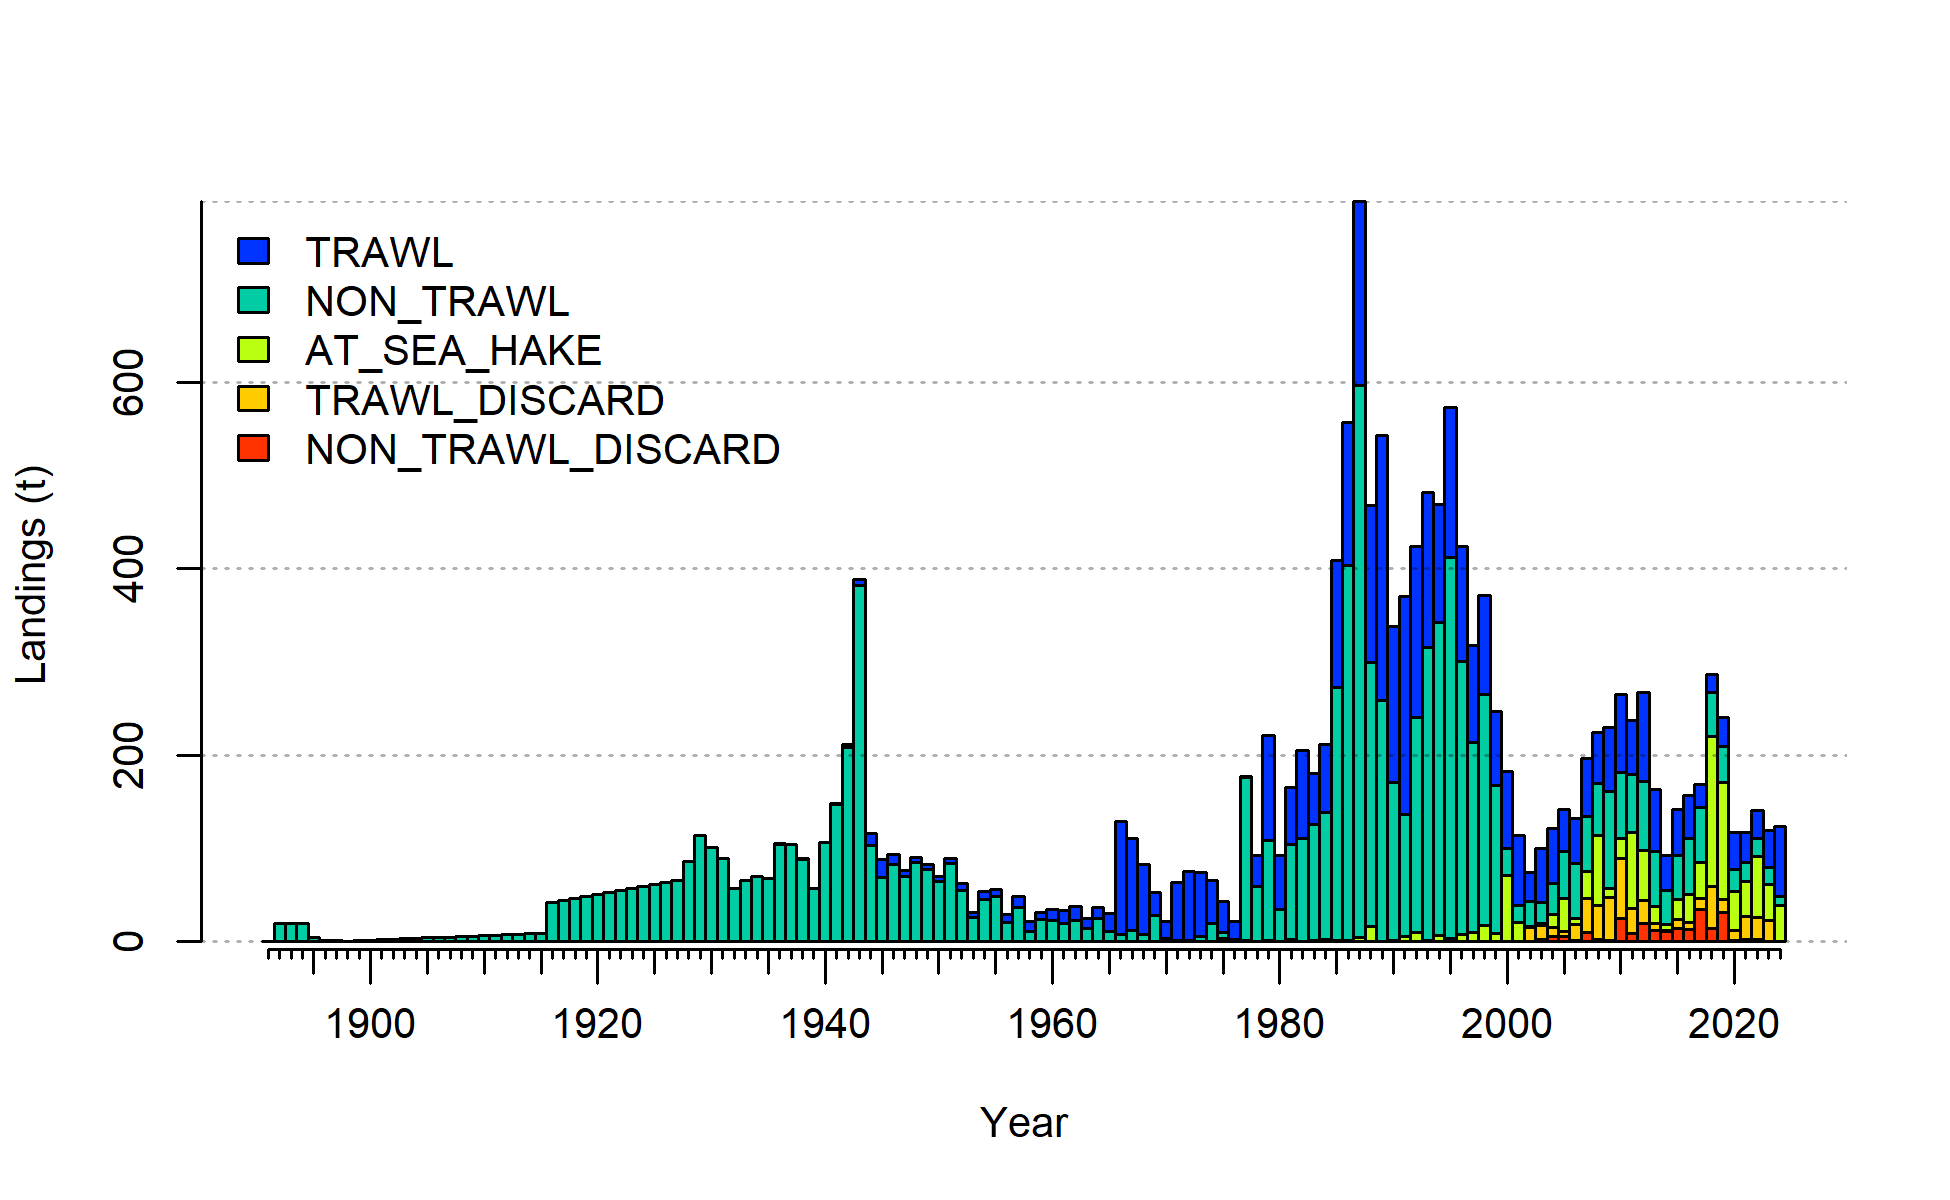
\includegraphics{ref_model/plots/catch2_landings_stacked.png}

}

\caption{\label{fig-es-landings}Landings in metric tons (mt) by year for
each fleet.}

\end{figure}%

\subsubsection{Data and Assessments}\label{data-and-assessments}

The only previous stock assessment for Rougheye/Blackspotted Rockfishes
for the west coast area was done in 2013. This assessment separates the
discard catches from the retained fisheries, maintains the at-sea-hake
fishery as its own fishery, and adds a midwater fishery that has emerged
in the last 10 years. This stock assessment adds 10+ years of additional
length data, and adds several more years of age data (included as
conditioned on length data). The same four groundfish abundance surveys
(Triennial, Alaska Slope, Northwest Fishery Science Center Slope, and
the West Coast Groundfish Bottom Trawl Survey (WCGBTS)) as used in the
last stock assessment are used here, with an extension to 2024 to the
the WCGBTS. The index standardization of all survey data uses the newer
approach of applying spatiotemporal generalized linear mixed models.

\subsubsection{Stock Output and
Dynamics}\label{stock-output-and-dynamics}

The model estimates that the population , but increased through the
2000s to mid 2010s (Figure~\ref{fig-es-sb}, Figure~\ref{fig-es-depl}).
Since 2017 (coincident with the increase in catches), spawning output
has been gradually declining, but is still well above the management
target of 40\% of unfished spawning depletion (Table~\ref{tbl-es-sb}).

\begingroup
\fontsize{9.0pt}{10.8pt}\selectfont

\begin{longtable}{>{\centering\arraybackslash}p{\dimexpr 56.25pt -2\tabcolsep-1.5\arrayrulewidth}>{\centering\arraybackslash}p{\dimexpr 56.25pt -2\tabcolsep-1.5\arrayrulewidth}>{\centering\arraybackslash}p{\dimexpr 56.25pt -2\tabcolsep-1.5\arrayrulewidth}>{\centering\arraybackslash}p{\dimexpr 56.25pt -2\tabcolsep-1.5\arrayrulewidth}>{\centering\arraybackslash}p{\dimexpr 56.25pt -2\tabcolsep-1.5\arrayrulewidth}>{\centering\arraybackslash}p{\dimexpr 56.25pt -2\tabcolsep-1.5\arrayrulewidth}>{\centering\arraybackslash}p{\dimexpr 56.25pt -2\tabcolsep-1.5\arrayrulewidth}}

\caption{\label{tbl-es-sb}Estimated recent trend in spawning output and
the fraction unfished and the 95 percent confidence intervals.}

\tabularnewline

\toprule
Year & Spawning output & Lower Interval (mt) & Upper Interval (mt) & Fraction Unfished & Lower Interval & Upper Interval \\ 
\midrule\addlinespace[2.5pt]
2015 & 4,980,880.00 & -2,394,229.28 & 12,355,989.28 & 0.882 & 0.648 & 1.115 \\ 
2016 & 4,969,040.00 & -2,407,010.06 & 12,345,090.06 & 0.880 & 0.644 & 1.116 \\ 
2017 & 4,954,860.00 & -2,421,248.86 & 12,330,968.86 & 0.877 & 0.638 & 1.116 \\ 
2018 & 4,939,980.00 & -2,435,854.46 & 12,315,814.46 & 0.875 & 0.633 & 1.116 \\ 
2019 & 4,914,880.00 & -2,461,228.86 & 12,290,988.86 & 0.870 & 0.623 & 1.117 \\ 
2020 & 4,893,940.00 & -2,484,344.42 & 12,272,224.42 & 0.867 & 0.615 & 1.118 \\ 
2021 & 4,891,640.00 & -2,492,249.92 & 12,275,529.92 & 0.866 & 0.613 & 1.119 \\ 
2022 & 4,895,270.00 & -2,498,752.93 & 12,289,292.93 & 0.867 & 0.613 & 1.121 \\ 
2023 & 4,900,640.00 & -2,508,886.25 & 12,310,166.25 & 0.868 & 0.612 & 1.123 \\ 
2024 & 4,913,820.00 & -2,516,893.46 & 12,344,533.46 & 0.870 & 0.614 & 1.126 \\ 
2025 & 4,929,120.00 & -2,527,915.77 & 12,386,155.77 & 0.873 & 0.615 & 1.130 \\ 
\bottomrule

\end{longtable}

\endgroup

\begin{figure}[H]

\centering{

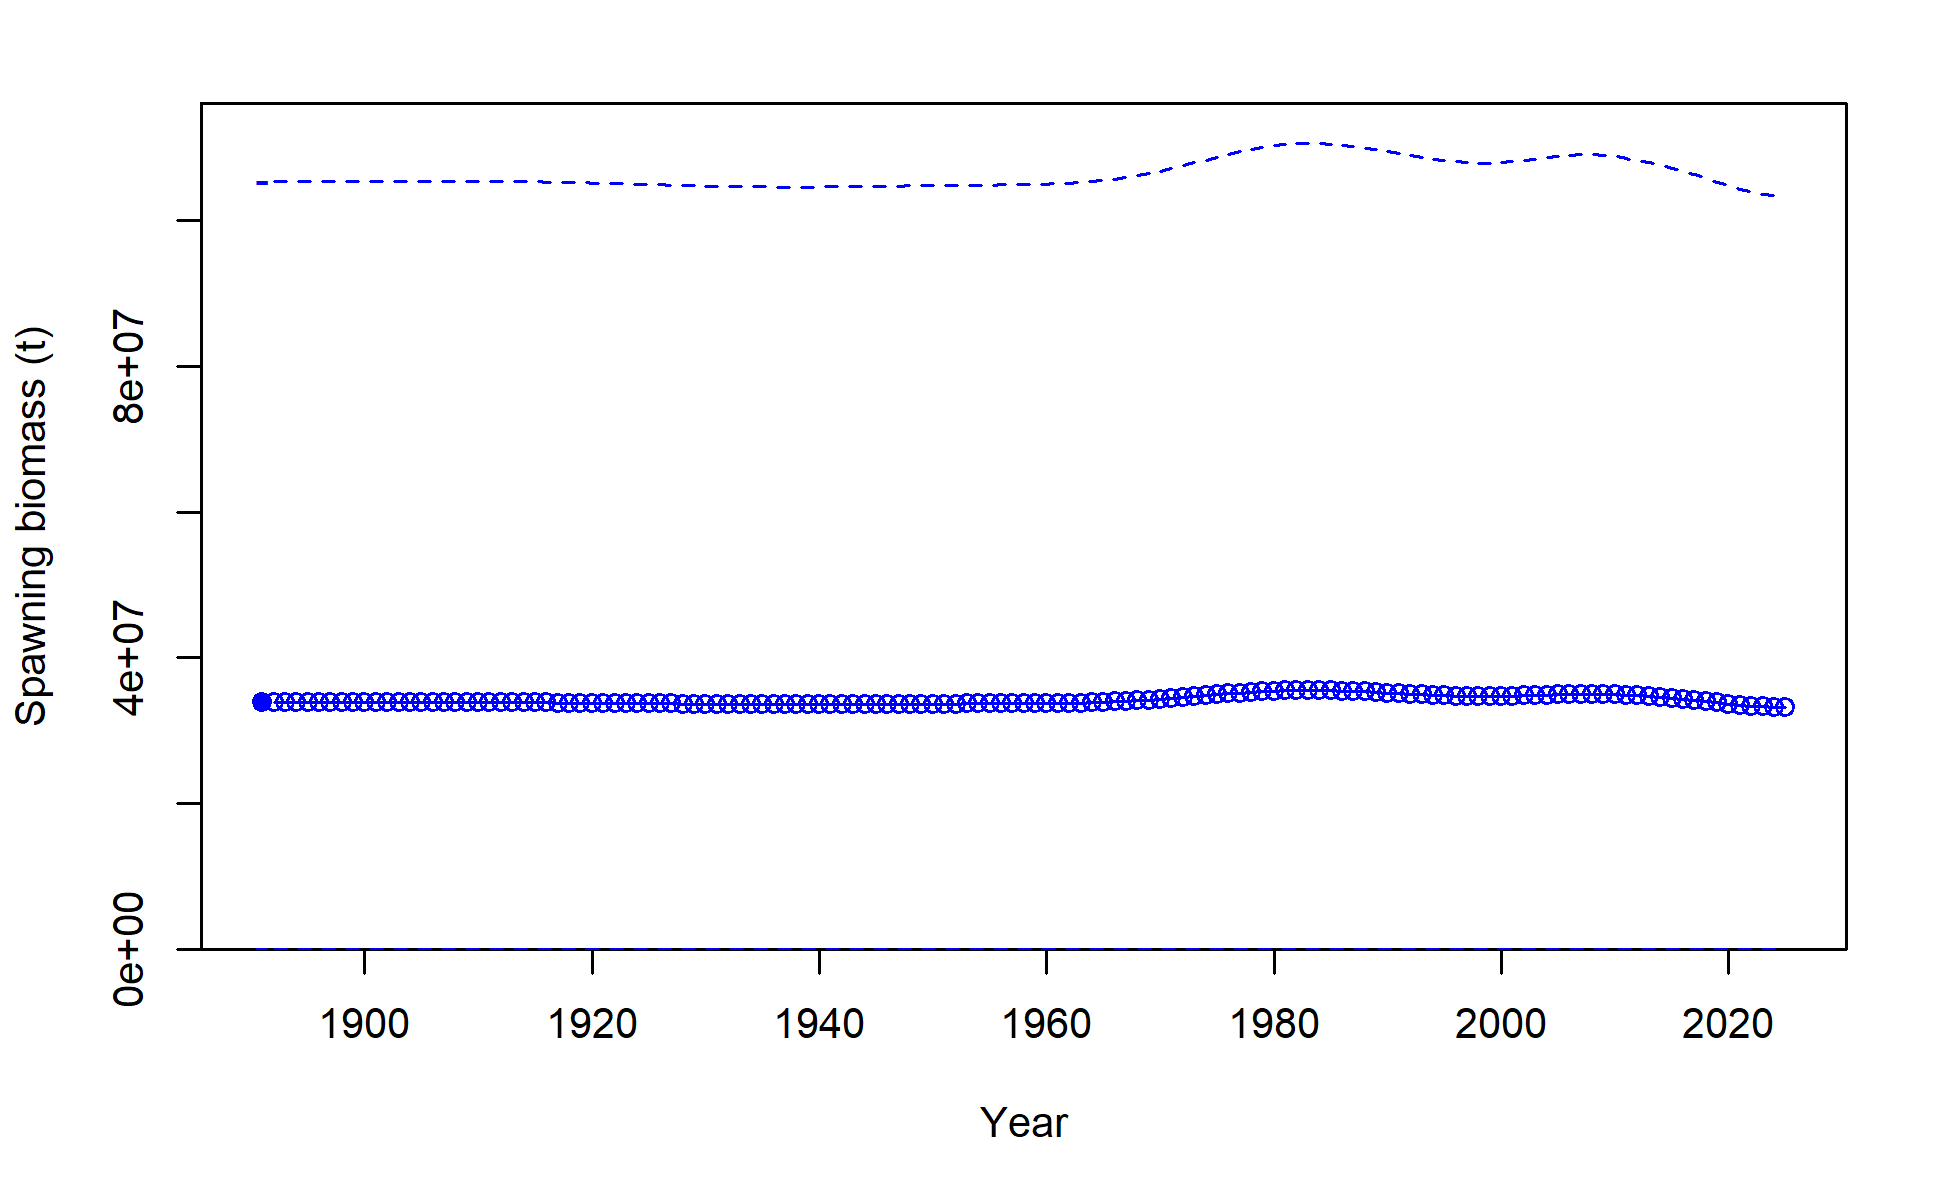
\includegraphics{ref_model/plots/ts7_Spawning_output_with_95_intervals.png}

}

\caption{\label{fig-es-sb}Estimated time series of spawning output
(trillions of eggs) for the base model.}

\end{figure}%

\begin{figure}[H]

\centering{

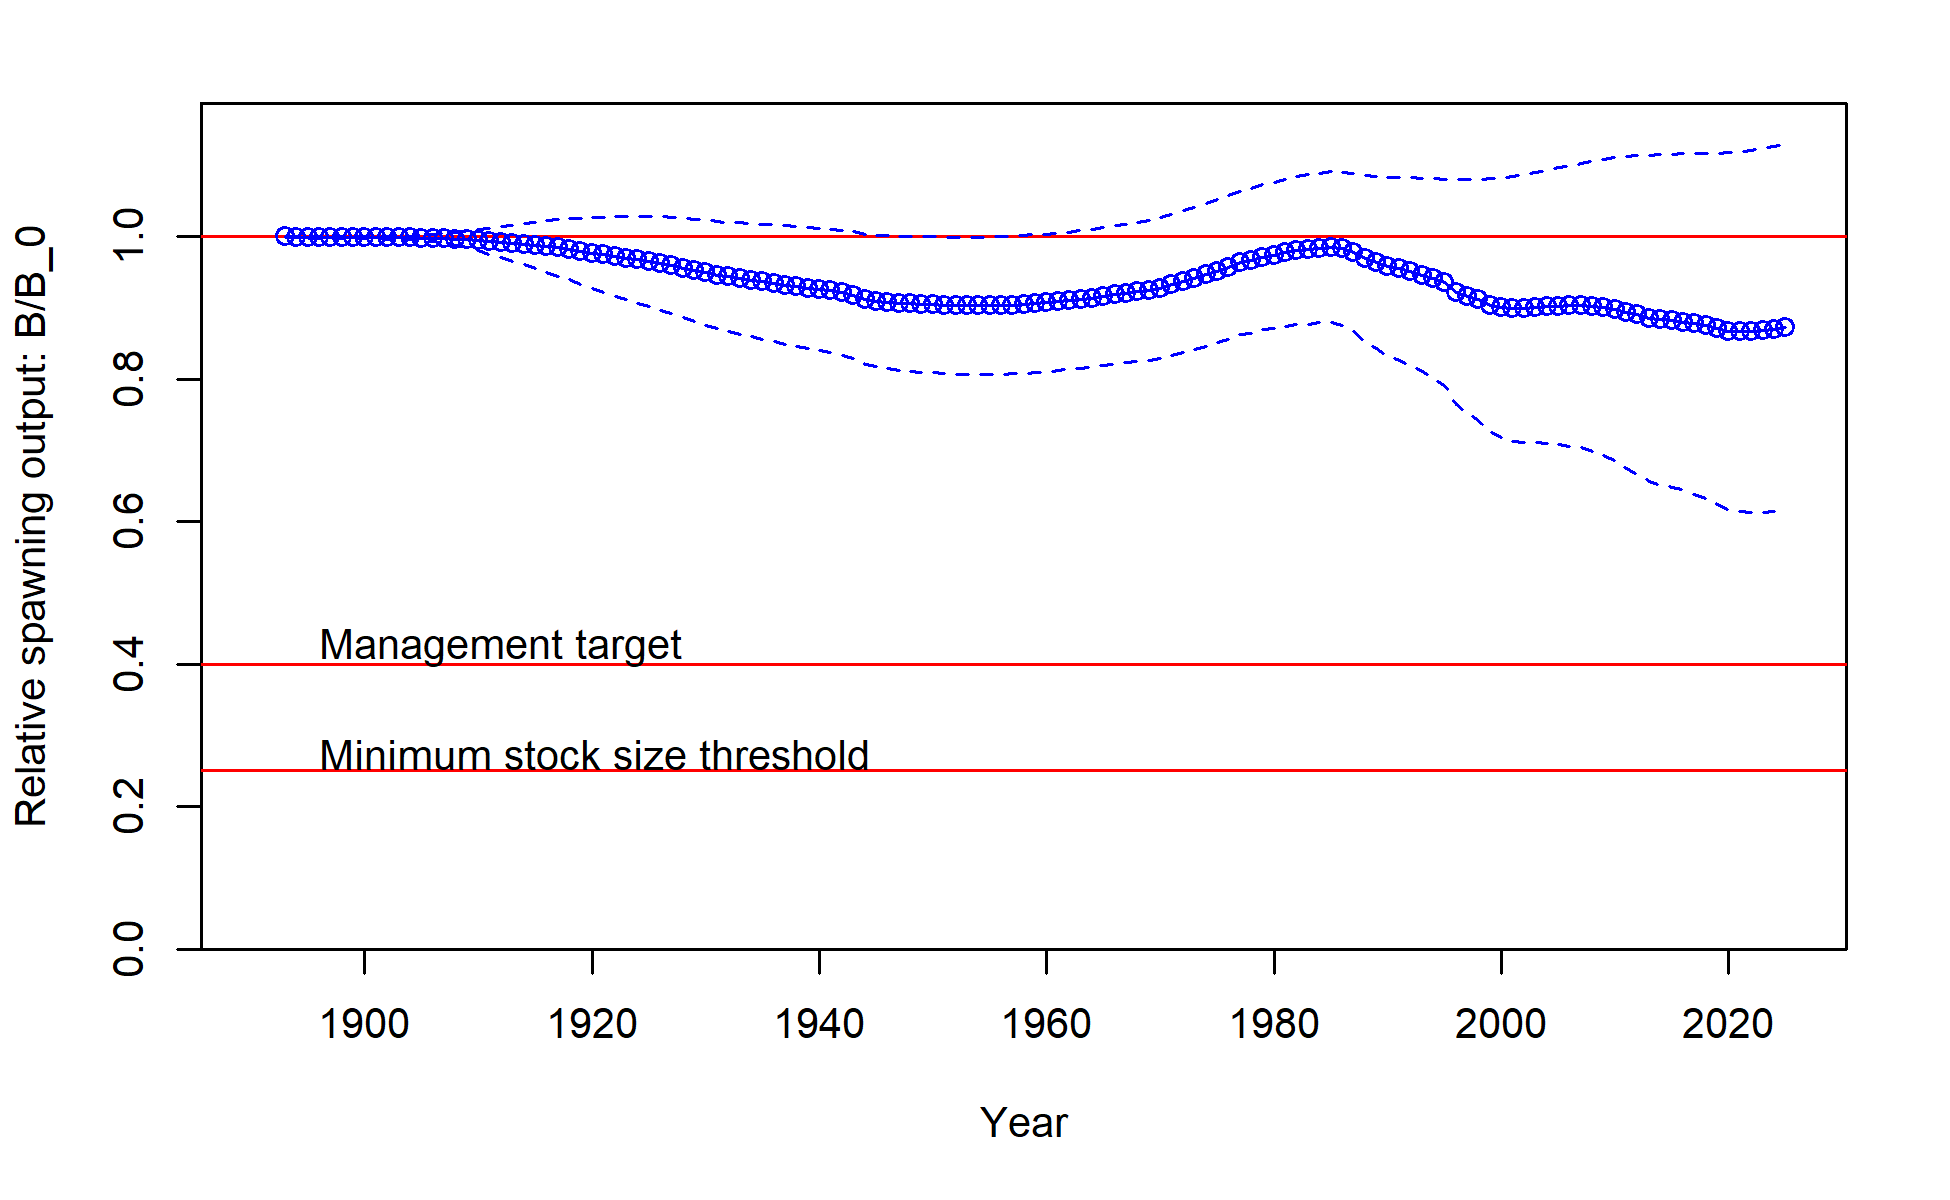
\includegraphics{ref_model/plots/ts9_Relative_spawning_output_intervals.png}

}

\caption{\label{fig-es-depl}Estimated time series of fraction of
unfished spawning output for the base model.}

\end{figure}%

\subsection{Recruitment}\label{recruitment}

The estimated largest recruitment event throughout the time series was
in 2008, which supported an increase in the population leading up to
2017 (Table~\ref{tbl-es-recr}, Figure~\ref{fig-es-recruits}).
Recruitment is estimated to be relatively low in the later 2010s, but
the model estimates that 2021 and 2023 may support large year classes in
the future, with the estimates driven by the new recruitment index for
both years.

\begingroup
\fontsize{9.0pt}{10.8pt}\selectfont

\begin{longtable}{>{\centering\arraybackslash}p{\dimexpr 56.25pt -2\tabcolsep-1.5\arrayrulewidth}>{\centering\arraybackslash}p{\dimexpr 56.25pt -2\tabcolsep-1.5\arrayrulewidth}>{\centering\arraybackslash}p{\dimexpr 56.25pt -2\tabcolsep-1.5\arrayrulewidth}>{\centering\arraybackslash}p{\dimexpr 56.25pt -2\tabcolsep-1.5\arrayrulewidth}>{\centering\arraybackslash}p{\dimexpr 56.25pt -2\tabcolsep-1.5\arrayrulewidth}>{\centering\arraybackslash}p{\dimexpr 56.25pt -2\tabcolsep-1.5\arrayrulewidth}>{\centering\arraybackslash}p{\dimexpr 56.25pt -2\tabcolsep-1.5\arrayrulewidth}}

\caption{\label{tbl-es-recr}Estimated recent trend in recruitment
(1,000s) and recruitment deviations and the 95 percent confidence
intervals.}

\tabularnewline

\toprule
Year & Recruitment (1,000s) & Lower Interval (1,000s) & Upper Interval (1,000s) & Recruitment Deviations & Lower Interval & Upper Interval \\ 
\midrule\addlinespace[2.5pt]
2015 & 659 & 173 & 2,515 & -0.445 & -1.271 & 0.382 \\ 
2016 & 870 & 228 & 3,328 & -0.172 & -1.012 & 0.668 \\ 
2017 & 2,172 & 584 & 8,071 & 0.738 & -0.009 & 1.484 \\ 
2018 & 1,341 & 354 & 5,087 & 0.251 & -0.565 & 1.066 \\ 
2019 & 1,197 & 317 & 4,517 & 0.132 & -0.678 & 0.943 \\ 
2020 & 846 & 221 & 3,242 & -0.220 & -1.083 & 0.643 \\ 
2021 & 923 & 236 & 3,608 & -0.138 & -1.050 & 0.774 \\ 
2022 & 1,017 & 254 & 4,067 & -0.046 & -1.008 & 0.916 \\ 
2023 & 1,067 & 266 & 4,286 & -0.003 & -0.982 & 0.975 \\ 
2024 & 1,076 & 268 & 4,323 & 0.000 & -0.980 & 0.980 \\ 
2025 & 1,076 & 268 & 4,324 & 0.000 & -0.980 & 0.980 \\ 
\bottomrule

\end{longtable}

\endgroup

\begin{figure}[H]

\centering{

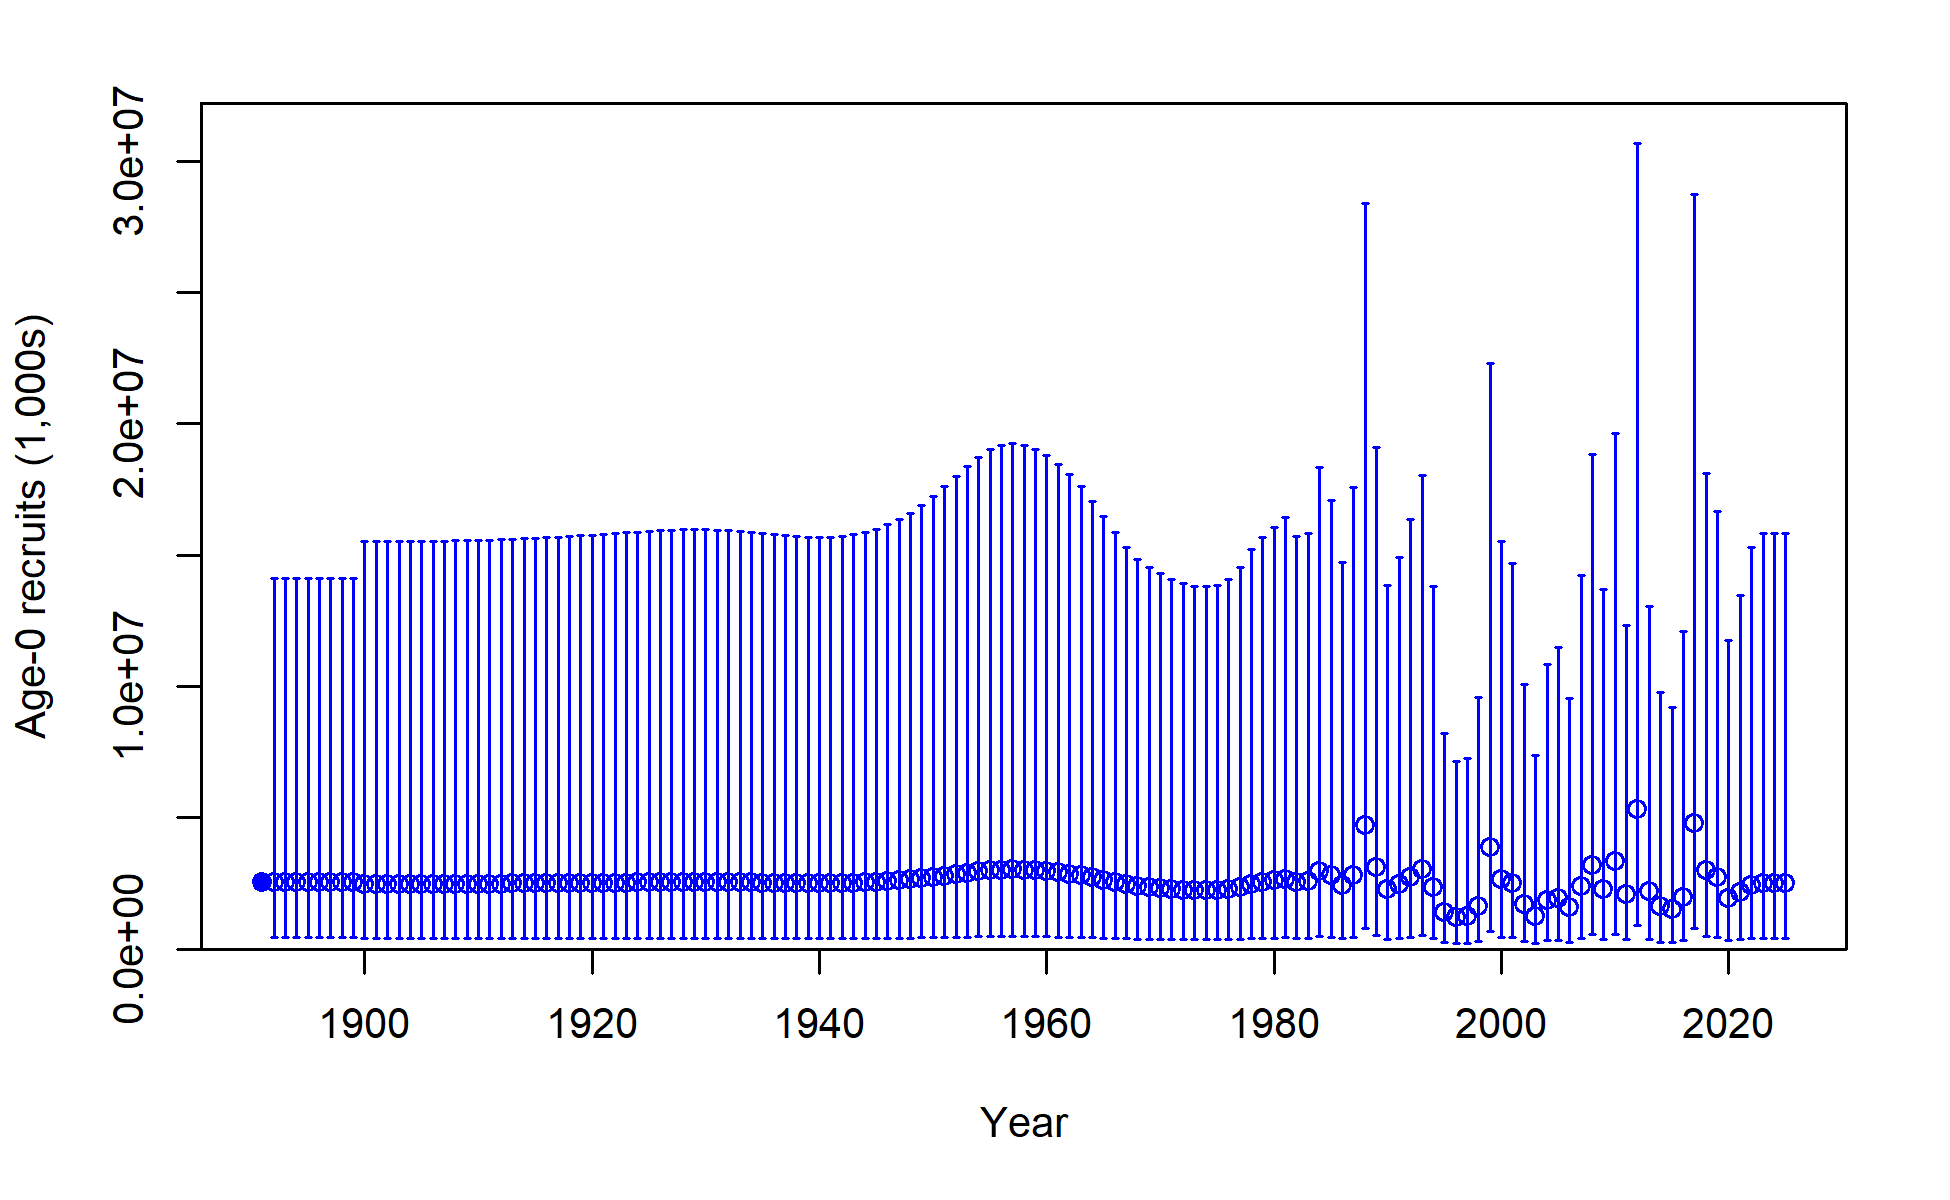
\includegraphics{ref_model/plots/ts11_Age-0_recruits_(1000s)_with_95_asymptotic_intervals.png}

}

\caption{\label{fig-es-recruits}Estimated time series of age-0 recruits
for the base model.}

\end{figure}%

\subsection{Ecosysystem Consideration}\label{ecosysystem-consideration}

The assessment includes a sensitivity model with an oceanographic
recruitment index. A number of ecosystem and environmental conditions
were compiled by a team of ecosystem scientists at the NWFSC specific to
the life history and distribution of northern yellowtail. These
conditions included an evaluation of oceanographic conditions impacting
recruitment, habitat change, prey availability, predator and competitor
abundance, and climate vulnerability.

\subsection{Reference Points}\label{reference-points}

A list of estimates of the current state of the population, as well as
reference points based on 1) a target unfished spawning output of 40\%,
2) a spawning potential ratio of 0.5, and 3) the model estimate of
maximum sustainable yield, are all listed in
Table~\ref{tbl-ref-points-es}. SPR, or the spawning potential ratio, is
the fraction of expected lifetime reproductive output under a given
fishing intensity divided by unfished expected lifetime reproductive
output.

\clearpage

\begingroup
\fontsize{9.0pt}{10.8pt}\selectfont

\begin{longtable}{lrrr}

\caption{\label{tbl-ref-points-es}Summary of reference points and
management quantities, including estimates of the 95 percent confidence
intervals. SO is spawning output, SPR is the spawning potential ratio,
and MSY is maximum sustainable yield.}

\tabularnewline

\toprule
Reference Point & Estimate & Lower Interval & Upper Interval \\ 
\midrule\addlinespace[2.5pt]
Unfished Spawning output & 5,647,660.0 & -1,285,869.4 & 12,581,189.4 \\ 
Unfished Age 26+ Biomass (mt) & 33,631 & -7,663 & 74,925 \\ 
Unfished Recruitment (R0) & 1,092 & -237 & 2,420 \\ 
2025 Spawning output & 4,929,120 & -2,527,916 & 12,386,156 \\ 
2025 Fraction Unfished & 0.873 & 0.615 & 1.130 \\ 
Reference Points Based SO40\% & — & — & — \\ 
Proxy Spawning output SO40\% & 2,259,070 & -514,338 & 5,032,478 \\ 
SPR Resulting in SO40\% & 0.458 & 0.458 & 0.458 \\ 
Exploitation Rate Resulting in SO40\% & 0.048 & 0.045 & 0.051 \\ 
Yield with SPR Based On SO40\% (mt) & 553 & -119 & 1,224 \\ 
Reference Points Based on SPR Proxy for MSY & — & — & — \\ 
Proxy Spawning output (SPR50) & 2,519,730 & -573,681 & 5,613,141 \\ 
SPR50 & 0.500 & — & — \\ 
Exploitation Rate Corresponding to SPR50 & 0.040 & 0.038 & 0.042 \\ 
Yield with SPR50 at SO SPR (mt) & 526 & -113 & 1,165 \\ 
Reference Points Based on Estimated MSY Values & — & — & — \\ 
Spawning output at MSY (SO MSY) & 1,497,160 & -343,313 & 3,337,633 \\ 
SPR MSY & 0.337 & 0.334 & 0.339 \\ 
Exploitation Rate Corresponding to SPR MSY & 0.085 & 0.079 & 0.090 \\ 
MSY (mt) & 592 & -127 & 1,311 \\ 
\bottomrule

\end{longtable}

\endgroup

\subsection{Management Performance}\label{management-performance}

Although catch increased substantially in 2017, it has still been well
below the overfishing limit, allowable biological catch, and annual
catch limit (Table~\ref{tbl-es-management}). Attainment of the OFL has
averaged around 50\% since the increase in landings, and was even lower
in prior years.

\begingroup
\fontsize{9.0pt}{10.8pt}\selectfont

\begin{longtable}{rcccr}

\caption{\label{tbl-es-management}Recent trend in the overfishing limits
(OFL), the acceptable biological catches (ABCs), the annual catch limits
(ACLs), and the total dead catch (landings + discards) all in metric
tons (mt).}

\tabularnewline

\toprule
Year & OFL (mt) & ABC (mt) & ACL (mt) & Total dead catch (mt) \\ 
\midrule\addlinespace[2.5pt]
2015 & NA & NA & NA & 132.09211 \\ 
2016 & NA & NA & NA & 148.95011 \\ 
2017 & NA & NA & NA & 156.01664 \\ 
2018 & NA & NA & NA & 241.51647 \\ 
2019 & NA & NA & NA & 226.59244 \\ 
2020 & NA & NA & NA & 106.07466 \\ 
2021 & NA & NA & NA & 92.76237 \\ 
2022 & NA & NA & NA & 117.42518 \\ 
2023 & NA & NA & NA & 97.62859 \\ 
2024 & NA & NA & NA & 118.93545 \\ 
\bottomrule

\end{longtable}

\endgroup

\subsection{Evaluation of Scientific
Uncertainty}\label{evaluation-of-scientific-uncertainty}

The largest uncertainty in this model is the inability to fit a marked
increase in the bottom trawl survey from 2014-2019. This coincides with
an increase in catch-per-unit-effort from the midwater trawl fishery
(which accounts for the majority of landings). The increase is likely
due to the record 2008 year class, but the estimated size of the year
class does not lead to a large enough increase to fit the survey index,
and it is especially hard to fit the sudden decrease and then flattening
of the index, given the estimated natural mortality rate and that
catches were relatively stable from 2017-2024. The current assessment
estimates that the stock is more depleted than it was in 2017, the time
of the last assessment, which is likely the case. The magnitude of that
difference is more uncertain.

\subsection{Harvest Projections and Decision
Tables}\label{harvest-projections-and-decision-tables}

Projections of the overfishing limit, acceptable biological catch, and
annual catch limit, all based on a P* of 0.45 and a log-space standard
deviation of the overfishing limit of 0.5 are included in
Table~\ref{tbl-es-projections}. Assumed catches for 2025 and 2026 for
this projection were provided by the Groundfish Management Team, and
catches from 2027 onward assume full attainment of the acceptable
biological catch.

\begingroup
\fontsize{9.0pt}{10.8pt}\selectfont

\begin{longtable}{>{\centering\arraybackslash}p{\dimexpr 56.25pt -2\tabcolsep-1.5\arrayrulewidth}>{\centering\arraybackslash}p{\dimexpr 56.25pt -2\tabcolsep-1.5\arrayrulewidth}>{\centering\arraybackslash}p{\dimexpr 56.25pt -2\tabcolsep-1.5\arrayrulewidth}>{\centering\arraybackslash}p{\dimexpr 56.25pt -2\tabcolsep-1.5\arrayrulewidth}>{\centering\arraybackslash}p{\dimexpr 56.25pt -2\tabcolsep-1.5\arrayrulewidth}>{\centering\arraybackslash}p{\dimexpr 56.25pt -2\tabcolsep-1.5\arrayrulewidth}>{\centering\arraybackslash}p{\dimexpr 56.25pt -2\tabcolsep-1.5\arrayrulewidth}>{\centering\arraybackslash}p{\dimexpr 56.25pt -2\tabcolsep-1.5\arrayrulewidth}>{\centering\arraybackslash}p{\dimexpr 56.25pt -2\tabcolsep-1.5\arrayrulewidth}>{\centering\arraybackslash}p{\dimexpr 56.25pt -2\tabcolsep-1.5\arrayrulewidth}}

\caption{\label{tbl-es-projections}Potential OFLs (mt), ABCs (mt), ACLs
(mt), the buffer between the OFL and ABC, estimated spawning output, and
fraction unfished with adopted OFLs and ACLs and assumed catch for the
first two years of the projection period.}

\tabularnewline

\toprule
Year & Adopted OFL (mt) & Adopted ACL (mt) & Assumed Catch (mt) & OFL (mt) & Buffer & ABC (mt) & ACL (mt) & Spawning output & Fraction Unfished \\ 
\midrule\addlinespace[2.5pt]
2025 & — & — & 968 & — & — & — & — & 4,929,120.000 & 0.873 \\ 
2026 & — & — & 955 & — & — & — & — & 4,841,850.000 & 0.857 \\ 
2027 & — & — & — & 942 & 0.935 & 880 & 880 & 4,760,140.000 & 0.843 \\ 
2028 & — & — & — & 930 & 0.930 & 865 & 865 & 4,690,410.000 & 0.831 \\ 
2029 & — & — & — & 919 & 0.926 & 851 & 851 & 4,624,410.000 & 0.819 \\ 
2030 & — & — & — & 908 & 0.922 & 837 & 837 & 4,561,470.000 & 0.808 \\ 
2031 & — & — & — & 897 & 0.917 & 823 & 823 & 4,501,170.000 & 0.797 \\ 
2032 & — & — & — & 886 & 0.913 & 809 & 809 & 4,443,180.000 & 0.787 \\ 
2033 & — & — & — & 876 & 0.909 & 796 & 796 & 4,386,880.000 & 0.777 \\ 
2034 & — & — & — & 865 & 0.904 & 782 & 782 & 4,331,770.000 & 0.767 \\ 
2035 & — & — & — & 854 & 0.900 & 769 & 769 & 4,277,630.000 & 0.757 \\ 
2036 & — & — & — & 843 & 0.896 & 756 & 756 & 4,224,160.000 & 0.748 \\ 
\bottomrule

\end{longtable}

\endgroup

\begin{Shaded}
\begin{Highlighting}[]
\DocumentationTok{\#\#| label: tbl{-}es{-}decision}
\DocumentationTok{\#\#| warning: false}
\DocumentationTok{\#\#| echo: false}
\DocumentationTok{\#\#| eval: !expr eval\_tables }
\DocumentationTok{\#\#| tbl{-}cap: !expr if(eval\_tables) decision\_table\_cap }
\DocumentationTok{\#\#| tbl{-}pos: H}

\CommentTok{\#table\_decision(}
\CommentTok{\#  list(mod\_low\_A, mod\_base\_A, mod\_high\_A),}
\CommentTok{\#  list(mod\_low\_B, mod\_base\_B, mod\_high\_B),}
\CommentTok{\# list(mod\_low\_C, mod\_base\_C, mod\_high\_C)}
\CommentTok{\#}
\CommentTok{\#}
\end{Highlighting}
\end{Shaded}

\subsection{Unresolved Problems and Major
Uncertainties}\label{unresolved-problems-and-major-uncertainties}

Test G

\subsection{Research and Data Needs}\label{research-and-data-needs}

Test H

\newpage{}

\setlength{\parskip}{5mm plus1mm minus1mm}
\pagenumbering{arabic}
\setcounter{page}{1}
\setcounter{section}{0}
\renewcommand{\thefigure}{\arabic{figure}}
\renewcommand{\thetable}{\arabic{table}}

\section{Introduction}\label{introduction}

This document presents the stock assessment for the Rougheye
(\emph{Sebastes aleutianus}) and Blackspotted (\emph{Sebastes
melanostictus}) rockfishes, two species that form one management
complex. This report is for the year 2025 in state and federal waters
from California to Washington State, excluding consideration of the
Puget Sound and Salish Sea (Figure~\ref{fig-map}). It seeks to use
available catch, biological compositions in the for of lengths and ages,
and potential indices of abundance and is the first assessment since the
2013 stock assessment (\citeproc{ref-hicks_status_2013}{Hicks, Wetzel,
and Harms 2013}).

\subsection{Stock Structure}\label{stock-structure}

There are at least two questions to think about when considering stock
structure for Rougheye and Blackspotted rockfishes when doing a stock
assessment.

\begin{enumerate}
\def\labelenumi{\arabic{enumi}.}
\tightlist
\item
  Rougheye and Blackspotted rockfishes are two different species-- can
  we separate them as two stocks and conduct separate assessments?
  Rougheye rockfish were first described in 1811 as \emph{Perca
  variabilis} by German zoologist Peter Simon Pallas
  (\citeproc{ref-jordan_fishes_1898}{Jordan and Evermann 1898}), and
  assigned to various taxa at least 15 times since
  (\citeproc{ref-love_rockfishes_2002}{Love, Yoklavich, and Thorsteinson
  2002}). Some descriptions noted both light and dark color morphs,
  which, along with possible confusion with several morphologically
  similar co-occurring species (e.g., \emph{S. borealis} and \emph{S.
  melanostomus}) have contributed to the persistent ambiguity in formal
  descriptions of Rougheye Rockfish (\citeproc{ref-orr_species_2008}{Orr
  and Hawkins 2008}). The first genetic studies conducted in the late
  1960s and early 1970s
  (\citeproc{ref-tsuyuki_contribution_1968}{Tsuyuki et al. 1968};
  \citeproc{ref-tsuyuki_analyses_1970}{Tsuyuki and Westrheim 1970})
  observed diversity suggestive of two genetic types within specimens
  identified as Rougheye Rockfish. Allozyme studies conducted over the
  next two decades (\citeproc{ref-seeb_biochemical_1986}{Seeb 1986};
  \citeproc{ref-hawkins_genetic_1997}{S. Hawkins, Heifetz, and Pohl
  1997}; \citeproc{ref-hawkins_genetic_2005}{S. L. Hawkins et al. 2005})
  provided additional evidence suggesting two separate genetic types
  within field-identified Rougheye Rockfish. Genetic variation between
  the two types, supported by both nuclear and mitochondrial DNA, was
  determined to be sufficiently conclusive to separate two species:
  ``Type I'' and ``Type II'' Rougheye Rockfish
  (\citeproc{ref-gharrett_two_2005}{Anthony J. Gharrett et al. 2005}).
  Meristic and morphometric comparisons of the two species suggested
  certain characters such as gill raker counts and length, snout length,
  anal base length, and pectoral fin base were significantly different,
  and in combination could reliably, though not definitively,
  distinguish between the
  species(\citeproc{ref-gharrett_genetically_2006}{A. J. Gharrett et al.
  2006}). The two separate species were formally re-described by Orr and
  Hawkins (\citeproc{ref-orr_species_2008}{2008}) with the Type II group
  retaining \emph{S. aleutianus} and the common name Rougheye Rockfish.
  Blackspotted rockfish was proposed as the common name for the Type I
  group along with the scientific name of \emph{S. melanostictus},
  re-establishing nomenclature from one of the species complex's earlier
  descriptions (\citeproc{ref-matsubara_1934}{Matsubara 1934}).
\end{enumerate}

These two species remain difficult to consistently differentiate
visually in the catch, thus are still commonly reported and treated as a
species complex. Otolith morphometrics (e.g., shape, size, weight) have
shown some promise in possibly identifying these species in Alaskan
waters (97.3\% Blackspotted and 86.2\% of Rougheye rockfishes were
accurately identified) and possibly using older otoliths to break out
historical information by species
(\citeproc{ref-harris_using_2019}{Harris, Hutchinson, and Wildes 2019}).
Frey et al.~(in prep.) provided insight into the ability of the
Northwest Fisheries Science Center West Coast Groundfish Bottom Trawl
Survey biologists to identify the two species, with 90\% of genetically
identified Rougheye rockfish being correctly identified in the field.
When mis-identifications occurred, it was usually a Blackspotted
rockfish being mis-identified as a Rougheye rockfish. There were few
mis-identifications when a fish was identified as a Blackspotted
rockfish. While this is promising for potential future species-specific
data coming from the survey, it does not alleviate the historical
problem of separating fishery data into the two species. Frey et al.~(in
prep.) therefore also considered whether ecological factors like depth
or latitude could help separate samples by species. They found that both
species occur within the range of this assessment's considered areas
(California to Washington), and heavily spatially overlap.
Interestingly, there seem to be relative hot spots for these species
where one species is more common than the other, and in general,
Rougheye rockfish seems to be more common than Blackspotted rockfish
(however, Blackspotted rockfish may be the more common of the two in
parts of Alaska; Anthony J. Gharrett et al.
(\citeproc{ref-gharrett_two_2005}{2005}); S. L. Hawkins et al.
(\citeproc{ref-hawkins_genetic_2005}{2005}); Orr and Hawkins
(\citeproc{ref-orr_species_2008}{2008})). Overall, there seems to be
little ability to separate current or historical fishery data reliably
in order to separate these two species into two stocks, so we will
maintain a species complex approach, though given absolute presence off
the U.S. West coast, this may be considered more of a Rougheye than
Blackspotted stock assessment. We also note that throughout the range of
these stocks, all current assessments to this point have maintained a
species complex approach.

Despite some identification advances and Rougheye and Blackspotted
rockfishes are clearly genetically distinct species, data historically
and contemporaneously remain available only for the
Rougheye/Blackspotted Rockfish complex, not at the species level. While
we treat these species as one assessed stock complex, we recognize and
are mindful of the above species distinctions as we conduct our
analyses.

\begin{enumerate}
\def\labelenumi{\arabic{enumi}.}
\setcounter{enumi}{1}
\tightlist
\item
  Both species range into Canada and Alaska-- are they one stock? While
  genetics studies have focused mostly on identification of the two
  species, little is known about the population structure of either
  species. This assessment and the 2013 assessment
  (\citeproc{ref-hicks_status_2013}{Hicks, Wetzel, and Harms 2013})
  represent the most southerly range of these species. Comparing the
  absolute abundance of the 2013 assessment to the most current
  estimates of the Alaskan stocks, the absolute number in this southerly
  range is much smaller than in the Gulf of Alaska (GOA), but higher
  than in the Bering Sea/Aleutian Island (BSAI) stock
  (Figure~\ref{fig-SO_comp}). The two smaller stocks have similar trend
  of decline and stabilization, whereas the higher biomass GOA stock
  looks to have not dropped at all over the time period considered
  (Figure~\ref{fig-RSS_comp}). We assume here that the west coast stocks
  of Rougheye/Blackspotted rockfishes are distinct management units from
  those in Alaska.
\end{enumerate}

\subsection{Life History}\label{life-history}

Rougheye and Blackspotted Rockfishes range from northern California up
to and throughout Alaska and into Japan
(\citeproc{ref-gharrett_two_2005}{Anthony J. Gharrett et al. 2005};
\citeproc{ref-hawkins_genetic_2005}{S. L. Hawkins et al. 2005};
\citeproc{ref-orr_species_2008}{Orr and Hawkins 2008}). Both are
long-lived (\textgreater100 years), with Rougheye Rockfish having the
distinction of the oldest ever aged \emph{Sebastes} species at 205 years
old. They both greatly overlap in latitude and depth (shallower than 100
m to at least 439 m), and are generally considered slope rockfish, with
an ontogenetic shift from shallower to deeper, and adults commonly found
at 360 m (around 200 fathoms). Rougheye seems to be proportionally more
abundant when survey samples are genetically identified, and
Blackspotted Rockfish tend to be found, on average, deeper than Rougheye
Rockfish (\citeproc{ref-hawkins_genetic_2005}{S. L. Hawkins et al.
2005}; \citeproc{ref-orr_species_2008}{Orr and Hawkins 2008}).

Rougheye/Blackspotted Rockfishes are often associated with structure,
such as hard, rocky bottoms and steep habitats. They are rarely found on
the deep flats. They can be found alone or in aggregations
(\citeproc{ref-love_rockfishes_2002}{Love, Yoklavich, and Thorsteinson
2002}), with aggregations often differentiated by age. Younger fish may
school and are often found in shallower waters on the shelf, junveiles
and subadults can be found together, and larger fish may form larger
aggregations in the Pacific Northwest during the autumn and winter.
These two species may also hybridize on occasion
(\citeproc{ref-love_certainly_2011}{Love 2011}). These species are
closely related to Shortraker Rockfish (\emph{S. borealis}) and are
sometimes difficult to distinguish from Shortraker Rockfish without
looking at the gill rakers. One major distinguishing feature of Rougheye
Rockfish are the 2--10 spines along the lower rim of their eyes, hence
the common name ``rougheye''.

Like all \emph{Sebastes} species, Rougheye and Blackspotted Rockfishes
give birth to live young. Larvae released has been documented between
February and June and extrusion lengths are between 4.5-5.3 mm
(\citeproc{ref-love_rockfishes_2002}{Love, Yoklavich, and Thorsteinson
2002}). There are no studies on the fecundity of rougheye rockfish on
the west coast of the U.S.

A wide range of prey items make up the diet of rougheye rockfish.
Crangid and pandalid shrimps make up the majority of their diets, and
larger individuals, greater than 30 cm, feeding upon other fishes
(\citeproc{ref-love_certainly_2011}{Love 2011}). They are also known to
feed upon gammarid amphipods; mysids, crabs, polychaetes, and octopuses
(\citeproc{ref-love_rockfishes_2002}{Love, Yoklavich, and Thorsteinson
2002}; \citeproc{ref-love_certainly_2011}{Love 2011}).

\subsection{Ecosystem considerations}\label{ecosystem-considerations}

\subsection{Historical and Current Fishery
Information}\label{historical-and-current-fishery-information}

Rougheye/Blackspotted Rockfishes are not often targeted by a specific
fishery, but are desirable and marketable, thus are typically retained
when captured. They are often captured in bottom trawl, mid-water trawl,
and longline fisheries. Small numbers have been observed in pot, shrimp,
and recreational fisheries.

After many attempts to start trawl fisheries off the west coast of the
United States in the late 1800's, the availability of the otter trawl
and the diesel engine in the mid-1920's helped the trawl fisheries
expand (\citeproc{ref-douglas_species_1998}{Douglas and Division 1998}).
The trawl fisheries really became established during World War II when
demand increased for shark livers and bottomfish. A mink food fishery
also developed during World War II
(\citeproc{ref-jones_oregon_1961}{Jones and Harry 1961}), and post-war
catches for rockfishes, including Rougheye/Blackspotted Rockfishes,
increased (\citeproc{ref-niska_species_1976}{Niska 1976}). Foreign
fleets began fishing for rockfish in the mid 1960's until the EEZ was
implemented in 1977 (\citeproc{ref-rogers_species_2003}{J. B. Rogers
2003}). Since 1977, landings of rockfish were high until management
restrictions were implemented in 2000. Longline catches of rougheye
rockfish are present from the turn of the century and continue in recent
years, targeting sablefish and halibut. The catches by state for the
trawl and hook \& line fleets as well as for the Pacific whiting at-sea
fleet are shown in ******.

A long-term directed fishery has not occurred for rougheye rockfish and
historical discarding practices are not well known. Rougheye rockfish
inhabit deeper water as adults, which were fished less often
historically. More detailed information of the fisheries by state is
given in Section ******* where the reconstructed landings are discussed.

\subsection{Management History and
Performance}\label{management-history-and-performance}

Rougheye/Blackspotted Rockfishes has been a small component of
groundfish fisheries and catches of Rougheye/Blackspotted Rockfishes
have been governed by restrictions on assemblages of species, of which
these species are a member. However, the distribution of fishing effort
in areas where Rougheye/Blackspotted Rockfishes might be encountered has
also been affected by catch restrictions on co-occurring, rebuilding
species, as well as associated area closures instituted to promote
rebuilding. The first imposed landings limits on a coastwide Sebastes
complex (Rougheye/Blackspotted Rockfishes being one of the 50 rockfishes
in the complex) were instituted in 1983. Ongoing concern that shelf and
slope rockfishes may be undergoing overfishing led the attempt by J. S.
Rogers et al. (\citeproc{ref-rogers_status_1996}{1996}) to describe the
status of most rockfishes contained in the Sebastes complex.
Rougheye/Blackspotted Rockfishes information content was low, and using
the Triennial survey to calculate an average biomass and assuming that
fishing mortality equals natural mortality provided estimates of
exploitation rates that indicated the stock was undergoing very high
exploitation rates in both management areas. The dividing line between
the northern and southern management areas was shifted to 40º 10' N
latitude in 1999 and the Sebastes complex was subsequently divided into
nearshore, shelf, and slope complexes in 2000. Rougheye/Blackspotted
Rockfishes has been managed under trip limits for the minor slope
rockfish complex in both north and south management areas since this
time.

Table (\citeproc{ref-management-summary}{\textbf{management-summary?}})
summarizes major management changes since 2000. Some important changes
include the implementation of Rockfish Conservation Areas (RCA's) in
2002, the beginning of trawl rationalization in 2011, and the lifting of
the RCAs beginning in 2020 with the removal of the trawl RCA in Oregon
and California and loosening restrictions in the non-trawl RCAs in 2023
and 2024.

Though managed as part of a complex, OFL contributions for
Rougheye/Blackspotted Rockfishes were calculated using DB-SRA in 2010
for the 2011-2012 management cycle. This lead to the observation that
recent catches had frequently exceeded the OFL contribution estimated
using data-poor, catch-only methods provided a strong indication that a
more thorough evaluation of Rougheye/Blackspotted Rockfishes stock
status and sustainable harvest levels be undertaken, using all available
data. A full assessment of Rougheye/Blackspotted Rockfishes was
undertaken in 2013 and indicated the stock complex was above management
target levels (Hicks, Wetzel, and Harms
(\citeproc{ref-hicks_status_2013}{2013})). Recent management performance
for Rougheye/Blackspotted Rockfishes as a part of the nothern minor
slope rockfish complex is provided in Table
(\citeproc{ref-managment-performance}{\textbf{managment-performance?}})
(ALI IS STILL CREATING THIS TABLE - WILL ADD TEXT FOR IT LATER).

\subsection{Fisheries off Canada and
Alaska}\label{fisheries-off-canada-and-alaska}

Rougheye Rockfish are distributed throughout Canada and Alaska and are
commonly caught in trawl and hook \& line fisheries. Alaska conducts
assessments biennially for the Rougheye/Blackspotted complex, and two
have been recently done: one for the Bering Sea and Aluetian Islands
(\citeproc{ref-spencer_assessment_2023}{Spencer, Ianelli, and Laman
2003}) and the other for the Gulf of Alaska
(\citeproc{ref-sullivan_assessment_2023}{Sullivan et al. 2023}). Canada
completed an assessment in 2020
(\citeproc{ref-starr_rougheyeblackspotted_2020}{Starr and Haigh 2020}).
The fisheries and assessments for each country are described below.

Rougheye rockfish have been managed as a bycatch only species in Alaska
since 1991 with catches ranging between 130 and 2,418 mt and peaking in
the late 1980s and early 1990s
(\citeproc{ref-sullivan_assessment_2023}{Sullivan et al. 2023}).
Generally, about 55-75\% of the catch are trawl-caught and 30-45\% from
hook-and-line (mainly, longline) fisheries. Since 2017 the move to pot
gear in the sablefish fishery has decreased the longline catches.
Discards since 2013 have ranged from 11.6\% (in 2023) and 45\% (in
2018). The Rougheye/Blackspotted complex catch levels generally are
between 20\% and 60\% of the Total Allowable Catch since the 2005 when
the complex began to be managed separately. The most recent
age-structured integrated stock assessments of this complex in the
Bering Sea and Aluetian Islands
(\citeproc{ref-spencer_assessment_2023}{Spencer, Ianelli, and Laman
2003}) and for the Gulf of Alaska
(\citeproc{ref-sullivan_assessment_2023}{Sullivan et al. 2023}) do not
indicate either overfishing or the stocks being overfished.

Canada identified two species of rougheye rockfish (Type I and Type II)
in 2007 and designated both species of special concern, which means that
they may become threatened or endangered because of a combination of
biological characteristics and identified threats
(\citeproc{ref-cosewic_2007}{Report 2007}). This designation was given
because biomass estimates are uncertain and no strong trends are
observed, there is evidence of truncation of the age distribution and
overall mortality has doubled, it is a long-lived, low-fecundity
Sebastes species, which is susceptible to population collapse and slow
recovery, and because the difficulty in separating the two species may
result in potential impacts on one of the species going unnoticed.
Subsequently, the species were identified as rougheye rockfish and
blackspotted rockfish and a management plan was created in 2012 with a
goal of sustaining the populations of rougheye and blackspotted
rockfishes
(\citeproc{ref-fisheries_and_oceans_canada_management_2012}{Canada
2012}). Five high priority and seven low priority actions have been
identified to address the threats to the populations and support the
management goal.

The first Canadian stock assessment for these species, using a
integrated catch-at-age model, was conducted in 2022 to estimated stock
status of two Rougheye/Blackspotted (REBS) rockfishes management units
(REBS north and REBS south) a the beginning of 2021. The REBS north
stock was in the healthy zone in the reference model. The REBS south
stock was likely in the healthy zone, but with an elevated possibility
of being in the cautious zone.

\newpage{}

\section{Data}\label{data}

Data from a wide range of sources were evaluated within this assessment.
Data sources included in the assessment model are summarized in
Figure~\ref{fig-data}. Description of each data source used in the model
is provided below.

\subsection{Fishery-dependent data}\label{fishery-dependent-data}

Rougheye/Blackspotted Rockfishes are not targeted by a specific fishery,
but are desirable and marketable, thus are typically retained when
caught. They are often captured in bottom trawl, mid-water trawl, and
longline fisheries. They are also commonly bycaught within the at-sea
hake fishery. Small numbers have been observed in pot and shrimp trawl.
Recreational catch is inconsequential and not accounted for in this
assessment.

Rougheye/Blackspotted Rockfishes fishery-dependent data in this
assessment are divided among six fleets, which include:

\begin{itemize}
\tightlist
\item
  Fleet 1: Commercial bottom trawl fishery.
\item
  Fleet 2: Dead discard from bottom trawl fishery.
\item
  Fleet 3: Commercial non-trawl (mainly the long-line) fishery.
\item
  Fleet 4: Dead discard from non-trawl fishery.
\item
  Fleet 5: Contemporary mid-water trawl fishery.
\item
  Fleet 6: At-sea hake fishery bycatch.
\end{itemize}

For description and details on fleet structure, please refer to Section
Section~\ref{sec-fleet}.

\subsubsection{Commercial Fishery
Landings}\label{commercial-fishery-landings}

Recent and historical fisheries catches were compiled by state and then
combined into the fishing fleets used in the assessment. Time series of
catches by fleet and state are reported in Table X.
Figure~\ref{fig-landings} shows catches by fleet.

\paragraph{Recent landings}\label{recent-landings}

Recent commercial landings of Rougheye/Blackspotted Rockfishes
(2000-2024 for Washington, 1987--2024 for Oregon and 1981--2024 for
California,) were obtained from PacFIN, a regional fisheries database
that manages fishery-dependent information in cooperation with West
Coast state agencies and National Marine Fisheries Service (NMFS). Catch
data were extracted from PacFIN on April 24, 2025.

\paragraph{Historical Landings}\label{historical-landings}

Historical landings of Rougheye/Blackspotted Rockfishes were
reconstructed by state.

The Washington historical landings (1889--2000) of Rougheye/Blackspotted
Rockfishes were provided by Washington Department of Fish and Wildlife
(WDFW), who recently conducted historical catch reconstruction for
rockfish species, including Rougheye/Blackspotted Rockfishes (pers.
comm. T. Tsou, WDFW). The three main sources used in this reconstruction
included the US Fish Commission Report (UFSC), Washington Bound Volumes,
and Washington Statistical Bulletin (SpeciesSumOutput2\_2017.csv- ADD
TABLE). The historical species composition was based on the various
historical reports and interviews of fishermen and dockside samplers.
The landings between 1981 and 2000 were also provided by WDFW (rather
than obtained from PacFIN), since WDFW developed and used a improved
method for apportioning unidentified rockfish (URCK) category in fish
tickets to the individual species landings. This improved approach
relaxed the borrowing rules for missing data used in the WDFW species
allocation algorithm that feeds into PacFIN (pers. comm. T. Tsou, WDFW).
New Washington historical landings represent improvement to the
assessment.

The Oregon historical landings (1896--1986) were obtained from Oregon
historical catch reconstruction, conducted by Oregon Department of Fish
and Wildlife (ODFW) in collaboration with NWFSC (Karnowski, Gertseva,
and Stephens (\citeproc{ref-karnowski_historical_2014}{2014})). The
Oregon landings for the period between 1987 and 1999 were also provided
by the ODFW. For that peios, Oregon PacFIN landings were supplemented
with the additional estimates of Rougheye/Blackspotted
Rockfisheslandings reported within unspecified rockfish market
categories, (i.e., URCK and POP1;
(\citeproc{ref-ODFW_URCK_POP_recon}{\textbf{ODFW\_URCK\_POP\_recon?}})).

The California historical landings were informed by several sources.
Landings from the most recent ``historical'' period (between 1969 and
1980) were obtaned from the California Cooperative Survey (CalCOM)
database. Earlier landing records (between 1931 and 1968) were informed
by the rockfish historical catch reconstruction conducted by the NOAA's
Southwest Fisheries Science Center (Ralston et al.
(\citeproc{ref-ralston_documentation_2010}{2010})).

Comparison of Rougheye/Blackspotted Rockfishes historical landings by
state and fleet between this and 2013 assessment is provided in
Figure~\ref{fig-Ct_All}. The largest differences in this assessment from
2013 model are in Washington landings (Figure~\ref{fig-Ct_WA}), with
newly estimated landings being generally lower than those used in
previous assessment. The new WDFW catch reconstruction completed by WDFW
is considered an improvement.

Historical California and Oregon landings did not change substantially
(Figure~\ref{fig-Ct_CA} and Figure~\ref{fig-Ct_OR}), with the exception
of a few years. Discrepancies in California and Oregon non-trawl
landings between the 2013 and 2025 assessments are caused by the fact
that non-trawl fleet in 2013 assessment was limited to only fixed gear,
when in 2025 assessment non-trawl fleet includes all non-trawl gear
groups. Slight discrepancies in Oregon trawl landings between 1987 and
1999, are from adding previously non-reported landings of
Rougheye/Blackspotted Rockfishes in the unspecified rockfish market
categories (see details above).

The update in historical changes shows only minor differences in model
outputs (Figure~\ref{fig-Ct_compsSO}; Figure~\ref{fig-Ct_compsRSS}).

\paragraph{Bycatch in the foreign POP
fishery}\label{bycatch-in-the-foreign-pop-fishery}

Between mid-1960s and mid-1970s, foreign trawl fleets from the former
Soviet Union, Japan, Poland, Bulgaria and East Germany targeted
aggregations of Pacific ocean perch in the Northeast Pacific Ocean, in
the waters off the U.S. West Coast (Love et al., 2002). Rogers (2003)
estimated removals of rockfish species caught within this foreign POP
fishery, including removals of Rougheye/Blackspotted Rockfishes. In the
assessment, Rougheye/Blackspotted Rockfishes bycatch in the foreign POP
fishery between 1966 and 1976 as estimated by Rogers (2003) were added
to commercial bottom trawl fleet.

\paragraph{At-Sea Hake Catches}\label{at-sea-hake-catches}

Rougheye/Blackspotted Rockfishes has long been bycaught in the fishery
for the coastal population of Pacific hake, which is almost exclusively
conducted with mid-water trawls.

Large-scale harvesting of Pacific hake in the United States began in
late-1960s, when factory trawlers from the Soviet Union and other
countries began targeting this stock. After the 200-mile U.S. Exclusive
Economic Zone was declared in 1977, a Joint-Venture fishery was
initiated between United States trawlers and Soviet factory trawlers
acting as mother-ships (larger, slower ships for fish processing and
storage while at sea). By 1989 the U.S. fleet capacity had grown to a
level sufficient to harvest the entire quota, and no further foreign
fishing was allowed. The Pacific hake fishery is currently 100\%
observed by the at-sea hake observer program (A-SHOP) and data on
bycatch species, including Rougheye/Blackspotted Rockfishes, is being
routinely collected.

Annual amounts of Rougheye/Blackspotted Rockfishes bycatch (retained and
discarded) in the Pacific hake fishery were obtained from the North
Pacific Database Program (NORPAC). That time series covers the period
between 1977 and 2024 and include catches by foreign and domestic
fisheries as well as removals during the time of Joint Ventures (JV).
Rougheye/Blackspotted Rockfishes catches within the at-sea hake fishery
were treated in the model as a separate fleet.

\subsubsection{Discards}\label{discards}

\paragraph{Historical discard}\label{historical-discard}

Historically, little to no discarding was observed for
Rougheye/Blackspotted Rockfishes.

The historical discard information comes from Pikitch et al.~(1988), and
often referred to as the Pikitch study. The Pikitch study was conducted
between 1985 and 1987 between 48°42' and 42°60' N. latitude, which is
primarily within the Columbia INPFC area (Pikitch et al.~1988).
Participation in the study was voluntary and included vessels using
bottom, midwater and shrimp trawl gears. Observers of normal fishing
operations on commercial vessels collected the data, estimated the total
weight of the catch by tow, and recorded the weight of species retained
and discarded in the sample.

There are no midwater trawl records of Rougheye/Blackspotted
Rockfishesin the Pikitch study, and only few fish records of bottom
trawl catches, based on which discard rate (discard weight over total
weight) for bottom trawl was just 0.09\%. Therefore, no historical
discard was assumed in the model.

\paragraph{Recent Discard}\label{recent-discard}

With the introduction of trip limits for rockfish in early 2000, limited
discard has been observed for Rougheye/Blackspotted Rockfishesin bottom
trawl and non-trawl fisheries.

In 2002, the West Coast Groundfish Observer Program (WCGOP) was
implemented on the West Coast of the United States, which began with
gathering bycatch and discard information for the limited entry trawl
and fixed gear fleets. Observer coverage has expanded to include the
California halibut trawl, the nearshore fixed gear and pink shrimp trawl
fisheries. Since 2011, trawl fisheries have been managed with catch
shares under a system of annual individual fishing quotas (IFQs) for the
shoreside sector (i.e., vessels delivering to shoreside processors) and
harvest cooperatives for the at-sea hake sectors (catcher-processors who
catch and process hake at sea; and Motherships, factory processors that
take delivery of hake from catcher vessels at sea). Constant monitoring
of catch using observers or electronic monitoring (EM) is required to
participate in the trawl catch share fishery.

The discard amounts of Rougheye/Blackspotted Rockfishes for the period
between 2002 and 2023 were obtained from WCGOP by year and fleet (bottom
trawl, mid-water trawl and non-trawl), for both the catch share and the
non-catch share sector. The discarding amounts of Rougheye/Blackspotted
Rockfishes within bottom trawl and non-trawl fleets were included in the
model as separate fleets.

Mid-water trawl discard was not present in non-catch share sector and
was extremely minimal (virtually non-existing) in catch-share sector,
with discard amounts averaging to 10kg per year. Therefore, in the
model, no discard was assumed for mid-water trawl fleet.

\subparagraph{Bottom Trawl Discard}\label{bottom-trawl-discard}

Bottom trawl discard amounts by year are provided in Table XX. Prior to
2011, before the start of the catch share program, the discard of
Rougheye/Blackspotted Rockfishes ranged between 1 metric ton and 60
metric tons, averaging at 23 metric tons a year. After 2011, the discard
has been very low, not exceeding 0.5 metric ton a year. No discard data
were available for 2024, and we used the average discard amount for 2019
- 2023 period to approximate 2024 discards for bottom trawl discard
fleet.

\subparagraph{Non-Trawl Discard}\label{non-trawl-discard}

Non-trawl discard amounts by year are provided in Table XX. Non-trawl
discard of Rougheye/Blackspotted Rockfishes were made in both catch
share and non-catch share sectors. Discard amounts in these sectors were
combined by year to represent total discard within the fleet. The
discards within this fleet ranged between 0.5 metric ton and 35 metric
tons, with 10 metric tons as average per year. No discard data were
available for 2024, and the 2023 discard amount was assumed for 2024 for
non-trawl discard fleet.

\subsubsection{Fishery Length and Age
Data}\label{fishery-length-and-age-data}

Length bins from 10 to 80 cm in 2 cm increments were used to summarize
the length frequency of the catches in each year. The first length bin
includes all observations less than 10 cm and the last bin includes all
fish 80 cm and longer. Age distributions included bins from age 1 to age
100, with the first bin including all fish ages 0 and 1 and the last bin
including all fish age 100 and above.

\paragraph{Commercial Landings Length and
Ages}\label{commercial-landings-length-and-ages}

The fishery length and age data for bottom trawl, non-trawl and midwater
trawl fleets, based on samples collected by port samplers, were obtained
from the PacFIN Biological Data System (BDS) database and extracted on
April 24, 2025. The number of trips and fish sampled for lengths and
ages by fleet and year are summarized in Tables XX-XX.

Commercial length-frequency distributions were developed for each fleet
and year, for which observations were available (Figire. Females and
males distributions were treated separately, to track sex-specific
differences. For each fleet, the raw observations were expanded to the
trip level, to account for differences in samples sizes relative catch
weights among trips (first stage expansion). The expanded length
observations were then further expanded to state level, to account for
differences in sampling intensity of Rougheye/Blackspotted Rockfishes
landings among states combined into a single fleet (second stage
expansion). The expansion algorithm can be illustrated with the
following equation:

\begin{centering}

$N_{b,j,y} = \displaystyle\sum_{s=1}^{s=k}\displaystyle\sum_{t=1}^{t=n}L_{b,j,t} \cdot
\left(\frac{LC_t}{SC_t}\right) \cdot \left(\frac{LC_{s,y}}{SC_{s,y}}\right)$

\end{centering}

Where \(N_{b,j,y}\) is the number of lengths in each length bin (\(b\))
by sex (\(j\)) and year (\(y\)) within each fleet. \(L_{b,j,t}\)
represents an individual length sample by bin (\(b\)) and sex (\(j\))
within an individual fishing trip (\(t\)). In the first stage expansion,
\(L_{b,j,t}\) was multiplied by the ratio of landed catch (\(LC_t\))
within that trip (\(t\)) to a portion of catch sampled for lengths
(\(SC_t\)) within the same trip (\(t\)). In the second stage expansion,
the individual length sample (\(L_{b,j,t}\)) was multiplied by the ratio
of landed catch (\(LC_{s,y}\)) within individual state (\(s\)) and year
(\(y\)) to catch weights sampled for lengths (\(SC_{s,y}\)) within the
same state (\(s\)) and year (\(y\)). As the final step, the expanded
length samples from the same size bin and sex were summed across all
trips and states (combined into a single fleet) within a single year, to
obtain the total number of lengths in each length bin by sex, year and
fleet (\(N_{b,j,y}\)). The same calculations were repeated for each
length bin, to develop sex specific length frequencies for each fishing
fleet by year.

Age distributions were included in the model as
conditional-age-at-length (CAAL) observations. The marginal
age-compositions were also included, but only for evaluating the implied
fits, while the CAAL data were used in the likelihood. The CAAL data
were not expanded and were binned according to length, age, sex, and
year.

The filtering and processing of the PacFIN length and age composition
data were conducted using the pacfintools package in R (Wetzel et
al.~2025). The filtering steps included removing samples with missing
vital information. Figures XX show the commercial length and age
frequencies used in the model for each fleet.

The initial input values for length compositions in this assessment were
calculated as a function of the number of trips and number of fish via
the Stewart Method (pers.comm. I. Stewart, International Pacific Halibut
Commission (IPHC)). The method is based on analysis of the input and
model derived effective sample sizes from West Coast groundfish stock
assessments. A piece-wise linear regression was used to estimate the
increase in effective sample size per sample based on fish-per-sample
and the maximum effective sample size for large numbers of individual
fish. The resulting equations are:

\begin{centering}

Input effN = $N_{\text{trips}} + 0.138 * N_{\text{fish}}$ if $N_{\text{fish}}/N_{\text{trips}}$ is $<$ 44

Input effN = $7.06 * N_{\text{trips}}$ if $N_{\text{fish}}/N_{\text{trips}}$ is $\geq$ 44

\end{centering}

The input sample size of CAAL data was set at the number of fish at each
length by sex and by year.

\subparagraph{Commercial Discard
Lengths}\label{commercial-discard-lengths}

Discard length composition data for both bottom trawl and non-trawl
discard fleets were available from WCGOP. Discard length composition
data were not sex-specific. Discard raw legnth observations were
expanded to the haul level, to account for differences in catch among
hauls.

The initial input values for length compositions were calculated via the
Stewart Method (see above).

No age data were available for discarded fish.

\subparagraph{At-sea hake Fishery Length and Age
Compositions}\label{at-sea-hake-fishery-length-and-age-compositions}

The sex-specific length and age data for at-sea hake fleet were
collected by the at-sea hake observer program (a-shop) and available
through NORPAC database. Input sample sizes for length compositions were
based on the number of hauls sampled by year.

Age distributions were included in the model as CAAL observations,
binned according to length, age, sex, and year. The input sample size of
CAAL data was set at the number of fish at each length by sex and by
year.

The marginal age compositions were constructed, but only used in the
model for evaluating the implied fits, while the CAAL data were used in
the likelihood.

\subsection{Fishery-independent data}\label{fishery-independent-data}

Data from four fishery-independent surveys were used in this assessment:

\begin{itemize}
\tightlist
\item
  West Coast Groundfish Bottom Trawl Survey (WCGBTS; 2003-2024)
\item
  AFSC/NWFSC West Coast Triennial (every three years) Shelf Survey
  (1980-2004)
\item
  Alaska Fishery Science Center Slope survey (1997, 1999-2001)
\item
  Northwest Fisheries Science Center Slope Center (1999-2002)
\end{itemize}

The surveys temporal and spatial coverage is summarized in Table XX.

Information produced by these surveys included indices of relative
abundance (all four surveys), length-frequency distributions (WCGBTS and
Triennial survey), and age-frequency distributions (WCGBTS).

Only the WCGBTS has new data for this assessment, but new methods were
applied to all surveys to develop new indices of abundance. In this
assessment, geostatistical models of biomass density were used to fit to
survey data using spatial and spatiotemporal GLMMs with TMB or
\href{https://pbs-assess.github.io/sdmTMB/}{sdmTMB}. The method is based
on a delta model. Two distributions (gamma and lognormal) were
considered for the catch-rate component. Comparing the standardized
versions (i.e., Z-scores, which puts all the indices on the same scale
for better comparison of trends) shows very similar trends among each
model output in the indices, suggesting little difference in choice of
model type. The lognormal error structure was selected for all surveys
because it was shown to be able to better account for extreme catch
events. The variance in the indices is generally high (0.3-0.5),
suggesting the information content in these indices is low. Overall,
catch densities are highest in northern Oregon and Washington.

Standardized indices for all four surveys overlaid are shown in
Figure~\ref{fig-All_indices}, where each index is rescaled to have mean
observation = 1.0.

Description of each survey is provided below; information available from
each survey and methods used to process the data are also discussed.

\subsubsection{NWFSC West Coast Groundfish Bottom Trawl
Survey}\label{nwfsc-west-coast-groundfish-bottom-trawl-survey}

\paragraph{Survey Description}\label{survey-description}

The West Coast Groundfish Bottom Trawl Survey (WCGBTS) is conducted
annually since 2003 (Table XX). The survey's design and sampling methods
are most recently described in Bradburn, Keller, and Horness
(\citeproc{ref-bradburn_2003_2011}{2011}). The survey is based on a
random-grid design, covering the coastal waters from a depth of 100 to
700 fm (183-1280 m). This design generally uses four industry-chartered
vessels per year assigned to a roughly equal number of randomly selected
grid cells and divided into two `passes' of the coast. Two vessels fish
from north to south during each pass between late May to early October.
This design therefore incorporates both vessel-to-vessel differences in
catchability, as well as variance associated with selecting a relatively
small number (approximately 700) of possible cells from a very large set
of possible cells spread from the Mexican to the Canadian borders.

\paragraph{Abundance Index}\label{abundance-index}

Geostatistical models of biomass density were fit to survey data using
spatial and spatiotemporal GLMMs with TMB or
\href{https://pbs-assess.github.io/sdmTMB/}{sdmTMB}(\citeproc{ref-kristensen_tmb:_2016}{Kristensen
et al. 2016}) via the R package \gls{sdmtmb}
(\citeproc{ref-Anderson:2022:SRP}{Anderson et al. 2022}) as configured
within the \{indexwc\} R package (Johnson et al.2025). Code to reproduce
the analysis is available online. These models can account for latent
spatial factors with a constant spatial Gaussian random field and
spatiotemporal deviations to evolve as a random walk Guassian random
field (J. T. Thorson et al.
(\citeproc{ref-thorson_geostatistical_2015}{2015})). Tweedie,
delta-binomial, delta-gamma, and mixture distributions, which allow for
extreme catch events, were investigated. Results are only shown for the
distribution that led to the best model diagnostics, e.g., similar
distributions of theoretical normal quantiles and model quantiles, high
precision, lack of extreme predictions that are incompatible with
yellowtail life history, and low AIC. Estimates of biomass from this
best model were predicted using a grid based on available survey
locations.

The data were truncated to depths less than 875 m prior to modelling
given that there were zero positive encounters in depths deeper than 875
m. The prediction grid was also truncated to only include available
survey locations in depths between 55-875 m to limit extrapolating
beyond the data and edge effects.

The model used a delta model with a lognormal distribution for the
catch-rate component. A logit-link was used for encounter probability
and a log-link for positive catch rates. The response variable was catch
(mt) with an offset of area (km\(^2\)) to account for differences in
effort. Fixed effects were estimated for each year. The following
additional covariates were included: pass. Vessel-year effects, which
have traditionally been included in index standardization for this
survey, were not included as the estimated variance for the random
effect was close to zero. Vessel-year effects were more prominent when
models did not include spatial effects and were included for each unique
combination of vessel and year in the data to account for the random
selection of commercial vessels used during sampling
(\citeproc{ref-helser_generalized_2004}{Helser, Punt, and Methot 2004};
\citeproc{ref-thorson_accounting_2014}{J. T. Thorson and Ward 2014}).

Spatial and spatiotemporal variation was included in the encounter
probability and the positive catch rate model. Spatial variation was
approximated using 400 knots, where more knots led to non-estimable
standard errors because the positive encounters are too sparse to
support the dense spatiotemporal structure.

The index is flat and is shown in Figure~\ref{fig-WCGBTS_index}.

\paragraph{Length and Age
compositions}\label{length-and-age-compositions}

Length bins from 1o to 80 cm in 2 cm increments were used to summarize
the length frequency of the survey catches in each year (Figure XX).
Table XX shows the number of lengths taken by the survey.

Length compositions were separated into males and females. These length
compositions were expanded to account for difference in catch among
tows, with further expansion based upon the stratification by depth and
latitude using the \{nwfscSurvey\} package in R
(\citeproc{ref-wetzel_nwfscsurvey_2023}{\textbf{wetzel\_nwfscsurvey\_2023?}}).
The stratification for length data expansions are provided in Table XX.

The input sample sizes for length composition data were calculated based
on Stewart and Hamel (\citeproc{ref-stewart_bootstrapping_2014}{2014})
as \(\text{Input N}_{y} = 2.43*N_{tow}\) where the 2.43 value was
estimated for a group of shelf and slope rockfish species.

Age distributions included bins from age 1 to age 100, with the last bin
including all fish of greater age. Table XX shows the number of ages
taken by the survey. Age distributions were included in the model as
CAAL observations. The marginal age compositions were only used for
comparing the implied fits, while the CAAL data were used in the
likelihood. The CAAL data were not expanded and were binned according to
length, age, sex, and year.

The input sample size of CAAL data was set at the number of fish at each
length by sex and by year.

\subsubsection{AFSC/NWFSC West Coast Triennial Shelf
Survey}\label{afscnwfsc-west-coast-triennial-shelf-survey}

\paragraph{Survey Description}\label{survey-description-1}

The Triennial Survey was first conducted by the AFSC in 1977 and
continued until 2004. The survey's design and sampling methods are most
recently described in \textbf{Weinberg et al.~(2002)}. Its basic design
was a series of equally-spaced transects from which searches for tows in
a specific depth range were initiated.

The survey spatial coverage and timing has changed over the period of
survey duration \textbf{(Table X)}.

Haul depths ranged from 91--457 m during the 1977 survey with no hauls
shallower than 91 m. The surveys in 1980, 1983, and 1986 covered the
West Coast south to 36.8°N latitude and a depth range of 55--366 meters.
The surveys in 1989 and 1992 covered the same depth range but extended
the southern range to 34.5°N (near Point Conception). From 1995 through
2004, the surveys covered the consistent depth range 55--500 meters and
surveyed south to 34.5°N. In the final year of the triennial series
(2004), the NWFSC conducted the survey and followed very similar
protocols as the AFSC, which conducted surveys in all previous years.

All of the surveys were conducted in the mid-summer through early fall:
the 1977 survey was conducted from early July through late September;
the surveys from 1980 through 1989 ran from mid-July to late September;
the 1992 survey spanned from mid-July through early October; the 1995
survey was conducted from early June to late August; the 1998 survey ran
from early June through early August; and the 2001 and 2004 surveys were
conducted in May-July \textbf{(Figure X)}.

Water hauls \textbf{(Zimmermann et al.~2003)} and tows located in
Canadian waters were also excluded from the analysis of this survey.
Given the different depths surveyed during 1977, the data from that year
were not included in this assessment.

\paragraph{Abundance Index}\label{abundance-index-1}

The index standardization followed a similar procedure to one used to
generate the WCGBTS index, when geostatistical models of biomass density
were fit to survey data using spatial and spatiotemporal GLMMs with TMB
or \href{https://pbs-assess.github.io/sdmTMB/}{sdmTMB}. The model used a
delta model with a lognormal distribution for the catch-rate component.
No pass covariate was included in the analysis since Triennial Survey
design did not include multiple passes.

The Triennial Survey was analyzed as an early series (1980--1992) and a
late series (1995--2004) to account for change in spatial coverage and
survey timing, as Rougheye/Blackspotted Rockfishesexhibit ontogenetic
movements when individuals gradually shift their distribution toward
deeper waters as the grow and mature. Separate catchability parameters
were estimated for pre-1995 period and from 1995 forward. Separate
selectivity curves were estimated for early and late survey periods as
well.

The estimated index is shown in Figure~\ref{fig-Triennial_index}. The
index exhibits an increase in biomass from 1995 forward, that
corresponds to a change in Triennial Survey depth coverage, when the
survye extended to the deeper area (Table XX)

\paragraph{Length Compositions}\label{length-compositions}

Length bins from 10 to 80 cm in 2 cm increments were used to summarize
the length frequency of the survey catches in each year (Figure XX).
Table XX shows the number of lengths taken by the survey.

Length compositions were separated into males and females. These length
compositions were expanded to account for difference in catch among
tows, with further expansion based upon the stratification by depth and
latitude using the \{nwfscSurvey\} package in R
(\citeproc{ref-wetzel_nwfscsurvey_2023}{\textbf{wetzel\_nwfscsurvey\_2023?}}).
The stratification for length data expansions are provided in Table XX.

The input sample sizes for length composition data for all
fishery-independent surveys were calculated based on Stewart and Hamel
(\citeproc{ref-stewart_bootstrapping_2014}{2014}) as
\(\text{Input N}_{y} = 2.43*N_{tow}\) where the 2.43 value was estimated
for a group of shelf and slope rockfish species.

There are no Rougheye/Blackspotted Rockfishes age data from the
Triennial Survey.

\subsubsection{AFSC Slope Survey}\label{afsc-slope-survey}

\paragraph{Survey Description}\label{survey-description-2}

The AFSC slope survey was initiated in 1984. The survey methods are
described in Lauth (2000). Prior to 1997, the survey was conducted in
different latitudinal ranges each year (Table 5). In this assessment,
only data from 1997, 1999, 2000 and 2001 were used -- these years were
consistent in latitudinal range (from 34°30' N. latitude to the
U.S.-Canada border) and depth coverage (183-1280 m; 100-700 fm).

\paragraph{Abundance Index}\label{abundance-index-2}

The index standardization followed a similar procedure to one used to
generate the WCGBTS and Triennial indeces, when geostatistical models of
biomass density were fit to survey data using spatial and spatiotemporal
GLMMs with TMB or \href{https://pbs-assess.github.io/sdmTMB/}{sdmTMB}.
The model used a delta model with a lognormal distribution for the
catch-rate component. As in case of Triennial survey, no pass covariate
was included in the analysis.

The AFSC Slope Survey index is shown in
Figure~\ref{fig-AFSC_Slope_index}. The index is short, and does not
exhibits significant change over the four year period.

\paragraph{Length Compositions}\label{length-compositions-1}

Length bins from 10 to 80 cm in 2 cm increments were used to summarize
the length frequency of the survey catches in each year (Figure XX).
Table XX shows the number of lengths taken by the survey.

Length compositions were separated into males and females. These length
compositions were expanded to account for difference in catch among
tows, with further expansion based upon the stratification by depth and
latitude using the \{nwfscSurvey\} package in R
(\citeproc{ref-wetzel_nwfscsurvey_2023}{\textbf{wetzel\_nwfscsurvey\_2023?}}).
The stratification for length data expansions are provided in Table XX.

The input sample sizes for length composition data for all
fishery-independent surveys were calculated based on Stewart and Hamel
(\citeproc{ref-stewart_bootstrapping_2014}{2014}) as
\(\text{Input N}_{y} = 2.43*N_{tow}\) where the 2.43 value was estimated
for a group of shelf and slope rockfish species.

There are no Rougheye/Blackspotted Rockfishes age data from the AFSC
Slope Survey.

\subsubsection{NWFSC Slope Survey}\label{nwfsc-slope-survey}

\paragraph{Survey Description}\label{survey-description-3}

The NWFSC slope survey was conducted annually from 1999 to 2002. The
survey's design and sampling methods are described in Keller et
al.(2007). The surveyed area ranged between 34°50' and 48°07' N.
latitude, encompassing the U.S. Vancouver, Columbia, Eureka, Monterey
INPFC areas, and a portion of the Conception area, and consistently
covered depths from 100 to 700 fm (183-1280 m) (Table XX).

\paragraph{Abundance Index}\label{abundance-index-3}

The index standardization followed a similar procedure to one used to
generate the other survey indeces, when geostatistical models of biomass
density were fit to survey data using spatial and spatiotemporal GLMMs
with TMB or \href{https://pbs-assess.github.io/sdmTMB/}{sdmTMB}. The
model used a delta model with a lognormal distribution for the
catch-rate component. No pass covariate was included in the analysis.

The NWFSC Slope Survey index is shown in
Figure~\ref{fig-NWFSC_Slope_index}. The index is short, and, as in case
of AFSC SLope Survey, does not exhibits significant change over the four
year period.

There are no Rougheye/Blackspotted Rockfishes length and age data from
the NWFSC Slope Survey. Given that spatial coverage of NWFSC Slope
Survey is the same of AFSC Slope Survey, selectivity of the NWFSC SLope
Survey was assumed the same as selectivity of AFSC Slope Survey
(mirrored in the model).

\subsection{Biological Parameters}\label{biological-parameters}

The major biological inputs to the models are natural mortality, age and
growth parameters, weight-length, maturity and stock-recruitment
parameters. The following sections outline the treatment of each
section. One change from the previous assessment is moving to a two sex
from the one-sex specification from 2013. The 2013 stock assessment
one-sex specification was based on the observation that the biology of
females and males was very similar, thus justifying the simplifying
assumption of one sex. The following sections below demonstrates that
females and males do generally have similar growth, though there are
differences, but may have different natural mortality values. The
current assessment will use a two sex configuration that allows for
flexibility to set female and male parameters either equal (i.e.,
functionally equivalent to a one sex model) and or sex-specific.
Figure~\ref{fig-Sex1vs2_SO} and Figure~\ref{fig-Sex1vs2_Bratio} show
that using a two sex configuration with the same life history parameters
for females and males is equivalent to the one sex model. Note that the
one sex model sums up both female and male biomass, thus why it is twice
the size as the two sex female-only spawning output
(Figure~\ref{fig-Sex1vs2_Bratio}).

\subsubsection{Natural Mortality}\label{natural-mortality}

Natural mortality is a highly influential parameter in age-structured
stock assessments. It defines the rate of natural death by age, and thus
establishes a stable age-structure and expectation of longevity, and
interacts with growth and reproduction to determine stock productivity.
It is a very difficult parameter to directly measure, thus empirical
relationships based on life history parameters are often used to
indirectly determine its value or build prior distributions in belief of
what it is in the event we do attempt to estimate it in the model (Cope
and Hamel (\citeproc{ref-cope_upgrading_2022}{2022}); Hamel and Cope
(\citeproc{ref-hamel_development_2022}{2022}); Maunder et al.
(\citeproc{ref-maunder_review_2023}{2023})). If length and age data are
available, it may be possible to estimate it in the model.

An estimate of maximum age tends to be the most reliable life history
parameter related to natural mortality to inform its estimation. Cope
and Hamel (\citeproc{ref-cope_upgrading_2022}{2022})
(\href{https://connect.fisheries.noaa.gov/natural-mortality-tool/}{The
Natural Mortality Tool}) provide the most up-to-date examination of the
relationship between maximum age and natural mortality

\begin{centering}

$M=\frac{5.4}{A_{\text{max}}}$

\end{centering}

\vspace{0.5cm}

where \(M\) is natural mortality and \({A_{\text{max}}}\) is the assumed
maximum age. The prior is defined as a lognormal distribution with mean
\(ln(5.4/A_{\text{max}})\) and standard error = 0.31. This is the
equation typically used to estimate a natural mortality point estimate,
but is underpinned by the choice of the value of \({A_{\text{max}}}\).
This equation assumes that the proportion of the stable population at
this maximum age is 0.4517\%. If we take humans as an example, the
longest lived human is 122 years. This is not the maximum age, but the
oldest ever recorded age. The maximum age that corresponds to 0.4517\%
of the population is around 100 years. For Rougheye/Blackspotted, the
oldest ever aged individual is 205 years with unknown ageing error. We
did not consider this as a realistic maximum age.

The 2013 U.S. west coast stock assessment used a prior built around a
mean of 0.034 (corresponding to a maximum age of 163), but estimated
natural mortality at 0.042 (maximum age between 128-129 years; Figure
M). The 2023 Gulf of Alaska assessment built a prior conditional on a
estimate of natural mortality from their 5 oldest aged individuals that
ranged from 126-135 years. This resulted in a mean value of 0.042,
similar to the 2013 U.S. west coast stock assessment. The 2023 Bering
Sea/Aleutian Islands assessment used M = 0.05 (assumed longevity of
108), and the recent Canadian assessments considered a range of M values
from 0.03 to 0.055 (assumed maximum ages of 180 to 98 years;
Figure~\ref{fig-Mcurves}).

We attempt to estimate natural mortality, as was done in the 2013 U.S.
West coast assessment. Examining the available age data, the oldest 10
individuals range from 139 to 165 and were all males. For females, the
10 oldest individuals range from 130 to 121 years. If those oldest ages
were used in the Hamel and Cope
(\citeproc{ref-hamel_development_2022}{2022}) longevity estimator, these
ages would correspond to a range of natural mortality values of 0.033 to
0.039 for males, which include the mean of the prior used in the 2013
assessment. For females, it corresponds to natural mortality values of
0.039 to 0.045. All these assume that the sampled population has enough
of an age structure still available for sampling, as opposed to having
some level of age truncation from the theoretical unfished stable age
distribution.

Related to this issue of possible age truncation, applying a catch curve
analysis (taking the log of the abundance of numbers of samples in
available age classes) on the aggregated ages across all age sources by
sex, the total mortality (Natural + Fishing mortality= Total mortality)
is 0.046 for females and 0.035 for males, which may indicate the natural
mortality could be lower than that used in the 2013 assessment, but
within the range of values considered in other areas
(Figure~\ref{fig-CC_Z}). This also indicates the possibility of
estimating sex-specific natural mortality, as natural mortality may
differ by sex. The two sex model allows for this type of model
specification exploration. Further exploration was done my truncating
the upper ages considered, with the assumption that the older ages may
also not be sampled fully (i.e., dome-shaped selectivity). We considered
both 100 (Figure~\ref{fig-CC_Z_100}) and 80 (Figure~\ref{fig-CC_Z_80})
as upper age cut-offs. The less older individuals included, the higher
the estimate of total mortality, and this a higher natural mortality.
But we can see a general overestimate of how many older individuals are
expected using these higher Z values, thus dome-shapeness does not see
to explain the sampling of these older individuals.

One challenge to estimating natural mortality within the model is the
interaction of estimating dome-shaped selectivity with estimating
natural mortality. If all fleets assume some level of dome-shaped
selectivity, it is difficult to determine if the unseen larger, older
individuals are due to natural death or fishing mortality. Typically, at
least one major fleet needs to achieve full selectivity for the larger,
older individuals. The 2013 assessment suggested some dome-shaped
selectivity in the two major fleets, thus any natural mortality
estimates are evaluated depending on the forms of fleet selectivity.

\subsubsection{Growth (Length-at-Age)}\label{growth-length-at-age}

Age and length data are used to estimate important growth parameters.
Figure~\ref{fig-AL_1} has the currently available age and length data.
Female and male sample sizes are very similar. Estimated growth curves
are also presented in Figure~\ref{fig-AL_1} and the parameters are
provided in Table AL\_1. The West Coast Groundfish Bottom Trawl Survey
clearly and importantly samples the smallest, youngest individuals
compared to the other two data sources. This allows for a better
estimate of the age at size 0 (t\textsubscript{0}) and growth
coefficient (k). The female asymptotic size
(L\textsubscript{\(\infty\)}) is estimated notably higher from the
PacFIN data, though male estimates of Linf are similar across the data
sets. The overall externally derived estimates of female and male
Rougheye/Blackspotted Rockfishes are

\begin{centering}

Females $L_{\infty}$ = 59.03 cm; $k$ = 0.07; $t_0$ = -2.45

Males $L_{\infty}$ = 56.69 cm; $k$ = 0.08; $t_0$ = -2.03

\end{centering}

The coefficient of variation (CV) of length by age and sex are shown in
Figure~\ref{fig-AL_2}. This is a measure of the variation in length for
a given age class. Sample sizes are highest from the youngest ages up to
around 70 (females) to 80 (males) years. The smoothed line shows the
average response, and indicates similar CVs values for females and
males, with the highest at the youngest ages, but generally 0.1. The
amount and range of age samples, along with repeated length samples
within an age class, allows growth parameters
(L\textsubscript{\(\infty\)}, k, t\textsubscript{0}, and CVs at age) to
be estimated in the model. Ages are conditioned on lengths in the model
in order to estimate growth within the model. We also explore
sensitivity in growth values by pre-specifying growth to different
values.

We note that the growth values being estimated in our data are notably
different than those used in Alaska. For instance, the growth parameters
for the BSAI stock is L\textsubscript{\(\infty\)} = 51.43, k = 0.06 and
t\textsubscript{0} = -3.30 and L\textsubscript{\(\infty\)} = 54.2 cm, k
= 0.07, t\textsubscript{0}= -1.5 for the GOA population (both sexes
combined). These growth parameters shows a larger size and faster growth
of the West Coast stock complex versus those in Alaska, though the West
Coast stock complex is more similar to the GOA complex.

\subsubsection{Ageing Bias and
Precision}\label{ageing-bias-and-precision}

Counting ages from ageing structures in long-lived, temperate fishes is
challenging. Ages derived from these structures can be hard to reproduce
within and between readers (i.e., imprecision), and may not contain the
true age (i.e., bias). Stock assessment outputs can be affected by bias
and imprecision in ageing, thus it is important to quantify and
integrate this source of variability when fitting age data in
assessments. In Stock Synthesis 3, this is done by including ageing
error matrices that include the mean age (row 1) and standard deviation
in age (row 2). Ageing bias is implemented when the inputted mean age
deviates from the expected middle age for any given age bin (e.g., 1.75
inputted versus 1.5 being the true age for the age 1 bin); ageing
imprecision is given as the standard deviation for each age bin.

There are eight primary readers that provided the available ages, two of
which often split the ageing duties. Figure~\ref{fig-AE_matrices} shows
which reader assignments are given to each year of ages by data source.
Reader 7 is the mix of two readers that shared reading duties within
years.

Estimation of ageing error matrices used the approach of -Punt et al.
(\citeproc{ref-punt_quantifying_2008}{2008}) in two different forms: one
developed in AD Model Builder
(\href{https://github.com/pfmc-assessments/nwfscAgeingError}{nwfscAgeingError}
(\citeproc{ref-thorson_nwfscageingerror:_2012}{J. T. Thorson, Stewart,
and Punt 2012})) and one adapted to Template Model Builder framework
(\href{https://pfmc-assessments.github.io/AgeingError/articles/getting_started.html}{TMB}).
The ageing error matrix offers a way to calculate both bias and
imprecision in age reads. Reader 1 is always considered unbiased, but
may be imprecise. Bias relative to the primary reader is given for the
second reader. There were three age readers that were assumed to be
unbiased. In those cases, 12 model configurations based on different
assumptions of imprecision (constant CV, curvilinear standard deviation,
or curvilinear CV, along with an option to either share or independently
estimate imprecision between readers) were considered. For the other
four age readers that could be biased and/or imprecise, thirty-six total
model configurations were explored that included the above imprecision
models as well as an exploration of the functional form of bias (e.g.,
no bias, constant coefficient of variation, or non-linear bias) in the
second reader.

Model selection criteria included AIC corrected for small sample size
(AICc), which converges to AIC when sample sizes are large, and Bayesian
Information Criterion (BIC). Both ADMB and TMB were run using an
(\href{https://github.com/shcaba/Ageing_Error_app}{ageing error shiny app}).
Model selection was then compared between ADMB and TMB, which did not
always agree, so model selection criteria was added across the two
modeling approaches to get an overall model selection criteria. Ageing
error matrices were also inspected for behavior in the best supported
models to make sure outrageously large precision or bias was not chosen
(effectively rendering the ages worthless, which is not an assumption of
the quality of the ages). Figure~\ref{fig-AE_bias} and
Figure~\ref{fig-AE_SD} show the bias and imprecision assumptions applied
for each ageing error (AE) matrix.

\subsubsection{Length-Weight
Relationship}\label{length-weight-relationship}

Female and male length-weight relationships were determined using data
from the PacFIN database, West Coast Groundfish Bottom Trawl Survey, and
ASHOP samples. Samples size by sex were: female (N=13839), males
(13625), and unknown sex (53). Each of the data sources estimated very
similar length-weight relationships (Figure~\ref{fig-LW1}).

The resultant sex-specific length-weight relationships are given in
Figure~\ref{fig-LW2}, with the following individual values:

\begin{itemize}
\tightlist
\item
  Females: W = 0.000008L\^{}3.15
\item
  Males: W = 0.000012L\^{}3.07
\end{itemize}

These values are very similar to the previous assessment that used a
combine sex value of a=0.0000096 and b=3.12000 (Figure~\ref{fig-LW2}).

\subsubsection{Maturity}\label{maturity}

Maturity for the Rougheye/Blackspotted Rockfish complex was estimated
using 473 maturity samples collected from 2015 to 2024 on gls\{odfw\}
and gls\{wdfw\} surveys and the gls\{indexwc\} in California, Oregon,
and Washington waters (M. Head, pers. comm.). The samples included 194
samples genetically assigned as Rougheye Rockfish, 71 samples
genetically assigned as Blackspotted Rockfish, and 208 samples with no
genetic assignment. The maturity schedule was assumed to be
length-based, as in the 2013 benchmark assessment. This assessment used
the functional classification of maturity to describe the maturity
schedule, which not only identifies the individuals that are
physiologically capable of producing yolk (those that are biologically
mature), but also accounts for the occurrence of abortive maturation and
skipped spawning, so the functional maturity classification is a more
accurate representation of the individuals that may actually spawn in a
given year. This is a difference from the 2013 benchmark assessment,
which did not explicitly estimate functional maturity, and instead
assumed the biological classification of maturity.

Biological maturity and functional maturity observations were fitted in
separate models. Biological maturity and functional maturity status
observations (0 = immature and 1 = mature) were fitted in a logistic
regression model (glm R function, family = binomial, link = ``logit'').
The estimated model parameters were used to calculate length at 50\%
maturity (L50\%; \textbf{Table XXX table Melissa provided}) and maturity
ogives (\textbf{Fig. XXX figure Melissa provided, the one comparing
biological and functional maturity}). The delta method was used to
calculate 95\% confidence intervals of L50\% estimates. The estimated
L50\% (functional maturity; L50\%fxn) was 46.53 cm and the estimated
slope of the maturity oogive was 0.25. Sensitivities were run using the
estimate of biological maturity and the maturity estimate used in the
2013 benchmark assessment. There was little evidence of skipped
spawning, so we did not explore fitting the data with a spline model.

Because there are known life history differences between Rougheye
Rockfish and Blackspotted Rockfish, maturity was also estimated for each
species, using the samples that were genetically assigned to each
species, respectively, using the same methods as above (\textbf{Table
XXX table Melissa provided and Figure XXX figure Melissa provided, the
one comparing overall functional maturity at length and for the two
species}). Two sensitivities were run using the functional maturity
L50\% (and slope) estimated for 1) Rougheye Rockfish and 2) Blackspotted
Rockfish (which mature at larger sizes on average than Rougheye
Rockfish).

Sensitivities were run using functional age at 50\% maturity estimate
for the species complex (n = 372) and for each species separately. Age
at 50\% maturity was estimated using the same methods as for length at
50\% maturity (\textbf{Table XXX table Melissa provided and Figure XXX
figure Melissa provided, the one comparing overall functional maturity
at age and for the two species}).

\subsubsection{Fecundity}\label{fecundity}

The 2013 U.S. west coast stock assessment assumed that fecundity was
proportional to weight. Dick et al.~(2017) provided a study on
rockfishes showing that rockfishes routinely have a non-proportional
relationship of fecundity to weight, with larger individuals producing
more eggs than expected only by weight. Neither Rougheye or Blackspotted
rockfishes have a species- of subfamily-specific estimate for this
relationship, so this stock assessment uses the unobserved Genus
Sebastes values of \(a\) = 6.538e-06 and \(b\) = 4.043 using the
F=aL\^{}b relationship. In order to adapt the \(a\) parameter for SS3,
the equation (a*10\^{}b)/1000 was used to scale the \(a\) parameter to
millions of eggs. This results in \(a\) = 7.218466e-05.

\subsubsection{Stock-Recruitment Function and
Compensation}\label{stock-recruitment-function-and-compensation}

The Beverton-Holt stock recruit relationship is assumed, as it was in
the 2013 assessment, to describe the relationship between spawning
biomass and recruitment. The steepness parameter may be considered for
estimation, but it is notoriously difficult to estimate in assessment
models. The 2013 stock assessment used the previous rockfish steepness
mean value of 0.77, but this has subsequently been updated to 0.72, to a
value that represents a stock with somewhat lower recruitment
compensation. Natural variation in recruitment (i.e., not
deterministically taken from the stock-recruit curve) is apparent in the
length and age data (as notable length or age classes growing/ageing
over time), so deviations in recruitment are estimated.

\subsubsection{Sex Ratio}\label{sex-ratio}

No information on the sex ratio at birth was available so it was assumed
to be 50:50.

\subsection{Environmental and ecosystem
data}\label{environmental-and-ecosystem-data}

This stock assessment does not explicitly incorporate trophic
interactions, habitat factors or environmental factors into the
assessment model. More predation, diet and habitat work, and mechanistic
linkages to environmental conditions would be needed to incorporate
these elements into the stock assessment and should remain a priority.
McClure et al. (\citeproc{ref-McClure:2023:VCC}{2023}) report the
climate vulnerability for several west coast groundfishes, including
Rougheye/Blackspotted Rockfishes. Rougheye/Blackspotted Rockfishes
demonstrated both high biological sensitivity and high climate exposure
risk, to give it an overall high vulnerability score to climate change.
This result should also be considered with the fact that, like many
rockfishes, periods of low productivity is not unusual to
Rougheye/Blackspotted Rockfishes and their extended longevity (though
admittedly this seems shorter than previously believed and should be
reconsidered) has historically allowed them to wait for advantageous
productivity periods. Stressors such as habitat degradation and climate
change could bring significant challenges to population sustainability.
Regardless, no environmental or ecosystem data are directly incorporated
into the stock assessment model.

\newpage{}

\section{Assessment}\label{assessment}

\subsection{History of Modeling
Approaches}\label{history-of-modeling-approaches}

Rougheye Rockfish (not including Blackspotted) on the U.S. Pacific Coast
was fist evaluated in 2010 by Dick and MacCall
(\citeproc{ref-dick_estimates_2010}{2010}) using depletion-based stock
reduction analysis (DB-SRA), as Category 3 stock. That model estimated
the population had greater than a 50\% probability of exceeding the
estimated proxy overfishing level in 2010 if the harvest remained at the
observed levels. DB-SRA estimated a proxy OFL for Rougheye Rockfish of
78.7 mt with a 95\% confidence interval between 4.7-587 metric tons.

Then,Rougheye/Blackspotted Rockfishes was assessment in 2013
(\citeproc{ref-hicks_status_2013}{Hicks, Wetzel, and Harms 2013}). A
2013 benchmark stock assessment used Stock Synthesis (version 3.24O)
integrated statistical catch-at-age model, which is different from the
delay-difference model with an assumed stock status prior DB-SRA
analysis used in 2010. The stock assessment has been used for management
as a Category 2 stock assessment. The 2013 assessment used a
substantially updated catch history, indices of abundance, and
biological compositions (lengths and ages). The natural mortality value
was also updated to be higher value than the one used in the DB-SRA
model. The 2013 assessment also assumed logistic selectivity for all
fleets and surveys, except for Triennial Shelf Survey, which was allowed
to be dome-shaped. With higher natural mortality and asymptotic
selectivity assumptions, the 2013 assessment estimated 2013 spawning
biomass to be at 47\% relative to unfished equilibrium spawning biomass,
with a 95\% confidence interval between 30.5\% - 64.2\%. The 2013
spawning biomass was estimated to be 2,552 metric tons, with a 95\%
confidence interval between 1,024 - 4,081 metric tons.

This benchmark assessment represent the first assessment of
Rougheye/Blackspotted Rockfishes since 2013
(\citeproc{ref-hicks_status_2013}{Hicks, Wetzel, and Harms 2013}). .

\subsection{Most Recent STAR Panel
Recommendations}\label{most-recent-star-panel-recommendations}

There were several recommendations from the 2013 STAR panel, broken into
two categories

\subsubsection{General recommendations}\label{general-recommendations}

\begin{enumerate}
\def\labelenumi{\arabic{enumi}.}
\tightlist
\item
  Investigate data-weighting options. \emph{This has been an ongoing
  research topic in stock assessments since this panel, and several
  options are no available for consideration.}
\item
  A workshop for constructing abundance indices from survey GLMMs.
  \emph{This is another topic that has developed greatly since this
  time. Our use of spatio-temporal models are described in the data
  section on abundance indices.}
\item
  Continue collection of ages. \emph{This had been done, and this
  assessment benefits from several more years of age data.}
\item
  Exploring historical catches. \emph{This again has been an ongoing
  topic and addressed for many of our groundfishes. We use the latest
  estimates in this assessment.}
\item
  SSC guidance on decision tables. \emph{Decision table discussion
  evolve after every stock assessment cycle, and we are using the latest
  approaches to decision tables in this assessment.}
\item
  Investigate fishery-independent slope surveys, such as submersibles.
  \emph{These surveys are not currently available for slope species.}
\end{enumerate}

\subsubsection{Stock-specific
recommendations}\label{stock-specific-recommendations}

\begin{enumerate}
\def\labelenumi{\arabic{enumi}.}
\tightlist
\item
  Collecting additional age data. \emph{This has been done and included
  in this stock assessment.}
\item
  Collecting genetic material to explore distinguishing Rougheye and
  Blackspotted Rockfishes. \emph{This work has been done as was
  presented earlier in the document when discussing stock structure
  decisions.}
\item
  The cause of the re-occurring decrease in sizes around 40cm.
\item
  Additional maturity and fecundity studies. \emph{While no fecundity
  studies are available, updated maturity is presented in the maturity
  section of the document.}
\item
  Age validation. \emph{While no age validation study has been
  completed, the agers are confident what annuli represent a year's
  worth of growth. Multiple ages are available and ageing error is
  characterized in this stock assessment.}
\item
  Understanding stock structure. \emph{Discussed in the stock structure
  section of this document.}
\item
  Connectivity of stocks across the species ranges. \emph{This is also
  discussed in the stock structure section of the document.}
\end{enumerate}

\subsection{Response to SSC Groundfish Subcommittee
Recommendations}\label{response-to-ssc-groundfish-subcommittee-recommendations}

\subsection{Current Modelling
Platform}\label{current-modelling-platform}

Stock Synthesis version 3.30.23.1 was used as the statistical
catch-at-age modelling framework. This framework allows the integration
of a variety of data types and model specifications. The Stock
Assessment Continuum tool (https://github.com/shcaba/SS-DL-tool) was
used also used to explore model efficiency, likelihood profiling,
retrospective analyses, and plotting sensitivities. The companion R
package r4ss (version 1.51.0) along with R version 4.4.3 were used to
investigate and plot model fits.

\subsection{Bridging the Assessment Model from Stock Synthesis 3.24
(2013) to 3.30
(2025)}\label{bridging-the-assessment-model-from-stock-synthesis-3.24-2013-to-3.30-2025}

More than 10 years have passed from the last assessment and in that
time, the model and the Stock Synthesis 3 (SS3) modelling framework has
undergone many changes. While the specific changes in the model can be
found in the model
\href{https://github.com/orgs/nmfs-ost/projects/11}{change log}, here we
simply update the model from the older 3.24O version to the newer
3.30.22.1 version. We want to ensure that any update to the newest SS3
model software is not a cause of any changes in model outputs when we
hold all data and model specifications to be exactly the same as in
2013. We therefore transferred all the older data and model
specifications to the newest version of SS3 and compared the outputs.
The status (Figure~\ref{fig-RSS_2013}) and scale
(Figure~\ref{fig-SO_2013}) of both models are exactly the same, as are
the estimates of within model uncertainty. This allows us to conclude
that we can move forward using the latest version of SS3 without concern
of inheriting any model output differences due to the choice of the SS3
version.

\subsection{Model Structure, Evaluation, and
Specification}\label{model-structure-evaluation-and-specification}

\subsubsection{Fleet and Survey Designations}\label{sec-fleet}

The model is structured to track several fleets and include data from
several surveys. Defining fleets is largely based on differing fleet
selectivity (i.e., how the fishery captures fish by length and/or age).
In the stock assessment model, selectivity translates into how the
removals are taken via length and/or age out of the population.
Currently, the following fleet structure is being used to model
commercial fishery removals as there is no record of a recreational
fishery for this stock complex:

\begin{itemize}
\tightlist
\item
  Fleet 1: Commercial trawl fishery
\item
  Fleet 2: Dead discard trawl
\item
  Fleet 3: Commercial fixed gear (mainly the long-line) fishery
\item
  Fleet 4: Dead discard non-trawl
\item
  Fleet 5: Contemporary mid-water fishery
\item
  Fleet 6: At-sea hake fishery
\end{itemize}

In 2013 assessment, fisheries removals were split among three fleets
--trawl, hook-and-line and at-sea hake fishery bycatch. For the first
two fleets (trawl and hook-and-line), removals were divided between
landings and discards, with selectivity and retention curves estimated
within the model.

For this assessment, we plan to treat discards in trawl and non-trawl
fisheries as separate fleets from landings fleets. This approach
provides several advantages, including:

\begin{itemize}
\tightlist
\item
  With separate discard fleets, we can easily track relative amounts of
  landings and discards within a fishery (they are not being combined
  into the total catch).
\item
  This approach provides more flexibility to explore different
  selectivity assumptions for both landed and discarded fish
  --dome-shaped vs asymptotic, mirroring one to the other, etc.
\item
  We can easily compare how similar (or different) selection curves for
  retained and discarded fish (easier than in case of selectivity and
  retention curves estimated within a single fleet), while avoiding hard
  to diagnose issues that come from estimating retention curves.
\item
  The biological data for landings and discards are collected
  independently (port sampling vs on-board observers), using different
  sampling approaches. Treating landings and discards as separate fleets
  in the model allows us to weight these data separately as well, to
  balance the representation of samples.
\end{itemize}

The change in treating discards as separate fleets does not impact model
results (Figure~\ref{fig-Discard_comp_SO} and
Figure~\ref{fig-Discard_comp_RSS}), regardless of the selectivity form
being assumed for the discard fleets. This provides evidence moving to
using discard fleets will not induce \emph{a prior} differences in the
model outputs, but it will offer more modelling flexibility.

We use length-based selectivity curves for all fleets for the current
stock assessment model (as was done in the 2013 assessment), as there is
no reason to believe significant age-based selectivity is occurring. We
consider logistic and dome-shaped selectivity options during reference
model development.

As reported in the data section, the following surveys are included in
the model:

\begin{itemize}
\tightlist
\item
  Survey 1: Triennial (every three years) survey (1980-2004)\\
\item
  Survey 2: Alaska Fishery Science Center Slope survey (1997-2001)
\item
  Survey 3: Northwest Fisheries Science Center Slope Center (1999-2001)
\item
  Survey 4: West Coast Groundfish Bottom Trawl Survey (WCGBTS;
  2003-2024)
\end{itemize}

The specifications of the assessment are listed in Table
\ref{tab:model-structure}.

\subsubsection{Model Likelihood
Components}\label{model-likelihood-components}

There are five primary likelihood components for each assessment model:

\begin{enumerate}
\def\labelenumi{\arabic{enumi}.}
\tightlist
\item
  Fit to length composition samples.
\item
  Fit to age composition samples (all fit as conditional age-at-length).
\item
  Fit to survey indices of abundance.
\item
  Penalties on recruitment deviations (specified differently for each
  model).
\item
  Prior distribution penalties
\end{enumerate}

In addition, there is a catch component to the likelihood, but catches
are essentially fit without error. Additionally, there is a crash
penalty that is invoked if true catches would cause the stock to go
extinct. The penalty would alter catches to avoid extinction, but any
presence of a crash penalty is used as in indication that the model has
been mispecified, so this likelihood contribution should always be 0.

\subsubsection{Reference Model Exploration, Key Assumptions and
Specification}\label{reference-model-exploration-key-assumptions-and-specification}

The reference model for Rougheye/Blackspotted Rockfishes was developed
to balance parsimony and realism, and the goal was to estimate a risk
neutral spawning output trajectory and relative stock status for the
stocks of Rougheye/Blackspotted Rockfishes in state and federal waters
off the U.S. west coast. To achieve the above goals, the model contains
uses different data types and sources to estimate reality, but relies on
simplifying assumptions when the data are not informative to parameters.
A series of investigative model runs were done to achieve the final
reference model. Constructing integrated models (i.e., those fitting
many data types) takes considerable model exploration using different
configurations of the following treatments:

\begin{itemize}
\tightlist
\item
  Data types and weighting
\item
  Parameter treatments: which parameter can, cannot and do not need to
  be estimated
\item
  Phasing of parameter estimation
\item
  Exploration of local minima vs global minimum (see Model Convergence
  and Acceptability section below)
\end{itemize}

Regarding data types, different biological data (i.e., length and/or age
composition) with and without the catch time series (and no additional
data weighting) were first included to obtain an understanding of the
signal of stock status coming from the data (Figure XXXXXX). The length
and age only models assume fixed life history values (growth fixed to
external estimates, natural mortality assume the reference model values)
and constant catch over the entire time series, while estimating the
selectivity of each fleet. Under this constraint, the lengths suggest a
stock status lower than the reference model, while the ages consider the
stock is less depleted than supported by the ages (with no ageing
error), and more similar to the reference model. Adding ageing error,
Putting the two data sources together produce an intermediate stock
status in the lower precautionary zone. Adding the catch time series
substantially changes the stock status trajectory, with length or age
only model above the reference stocks status. Combining the two came out
just under the reference model. Only one model includes recruitment
deviations, and demonstrates more dynamics behavior similar to that seen
when biological compositions are unweighted (see Model Specification
Sensitivities section ).

Stock scale was comparable once removal history was included, and
demonstrates a large sensitivity to the scale of the stock given the
data with no additional weighting included (Figure ).

Numerous exploratory models that included all data types and a variety
of model specifications were subsequently explored and too numerous to
fully report. In summary, the estimation of which life history
parameters to estimate and fix was liberally explored.

The following is a list of things that were explored, typically in
combination with one another

\begin{itemize}
\tightlist
\item
  Estimate or fix \(M\)
\item
  Estimate or fix any of the three growth parameter for each sex
\item
  Estimate or fix the stock-recruit relationship
\item
  Estimate or assume constant recruitment. If estimating recruitment,
  for what years?
\item
  Estimate additional survey variance, and for which survey?
\item
  Logistic or dome-shaped selectivity?
\item
  Estimate or fix selectivity parameters
\end{itemize}

All growth parameters were estimable and did not change across the large
majority of explored model scenarios, so they were estimated in the
reference model. Natural mortality (\(M\)) was not estimable for both
sexes. When attempted, both values were estimated at values that caused
the scale to approach the higher end of reasonable values, and thus not
a risk neutral option. In order to balance model fit and reality, a
likelihood profile was conducted on natural mortality for males (females
\(M\) being estimated) in order to find the lowest supported (i.e.,
within 2 negative log likelhood units) by the data male \(M\) value. The
profile shows conflicting information in the data, where lengths support
higher natural mortality values and ages support lower natural mortality
(Figure~\ref{fig-M-profile-explore}). It is expected that ages would be
more informative to natural mortality, which encourages considering just
the age component likelihood. Most of the age components are not well
informed for natural mortality, though the at-sea-hake fishery sampled
age data does seem to be informative. This fishery has a logisitic
selectivity, thus obtaining large and old individuals. Using this
component likelihood, the value of 0.036 for male \(M\) is the lowest
value supported. The reference model this fixes male \(M\) to this value
and estimates female \(M\). Length-at-maturity, fecundity-weight, and
length-weight relationship were all fixed, as is the only treatment
option in SS3.

For recruitment, steepness (\(h\)) was not estimable and was fixed to
the rockfish prior of 0.72. Recruitment variability was set at 0.5 and
checked for consistency with the calculated recruitment variability in
the model. Recruitment deviations were estimated as a deviation not
constrained to sum to 0, and initially estimated for the full time
series. If the full time series was not estimated, the scale and status
of the stock increased to unrealistically high levels, so the full time
series estimation was retained. Given the longevity of these species,
information on recruitment going deeper into the time series is not
unreasonable.

The selectivity of all fisheries and surveys were estimated either as
logistic or dome-shaped selectivity. Blocks were also added as described
in the data section. In the attempt to fit the biological data, it was
found that bottom trawl fisheries, just as the trawl surveys were
treated, only fit the data if the selectivity was domed. All fisheries
that had final dome-shaped selectivity were given the flexibility to be
logistic if it led to a better fit. The midwater, at-sea-hake and the
final block of the non-trawl fisheries all required logistic selectivity
to fit the data. The use of dome-shaped selectivity for the bottom trawl
was a major difference from the previous stock assessment. The choice of
selectivity for the bottom trawl survey changed the scale and status of
the stock and therefore a major source of sensitivity.

The full list of estimate and fixed parameters are found in
Table~\ref{tbl-param}.

The biggest uncertainty was in the treatment of sex-specific \(M\) and
the selectivity of the bottom trawl fishery. The combination of these
two sources covered the extent of all other sources of uncertainty
observed and presented in the ``Characterizing uncertainty'' section of
the document. The parameters uncertainty is different than the
uncertainty derived from data treatment, such as ageing error and
data-weighting. While these issues cause large uncertainty in stock
scale and status estimates, the choice of treatments are based on the
common challenge of balancing information content (i.e., what should the
data be informing in the stock assessment) in the data within an
integrated statistical frameworks. Those explorations are also provided
in the ``Characterizing uncertainty'' section.

General attributes of the reference model are that indices of abundance
are assumed to have lognormal measurement errors. Length compositions
and conditional age at length samples are all assumed to follow a
multinomial sampling distribution, where the sample size is fixed at the
input sample size calculated during compositional example, and where
this input sample size is subsequently reweighted to account for
additional sources of overdispersion (see below). Recruitment deviations
were also estimated are assumed to follow a lognormal distribution,
where the standard deviation of this distribution is tuned as noted
above.

Sensitivity scenarios and likelihood profiles (on \(lnR_0\), steepness,
and natural mortality) were used to explore uncertainty in the above
model specifications and are reported in the ``Characterizing
uncertainty'' section.

\subsubsection{Data Weighting}\label{data-weighting}

Initial sample sizes for the length and conditional age-at-length
compositions were also considered for additional data-weighting. The
method of Francis (\citeproc{ref-francis_data_2011}{2011}), specifically
equation TA1.8, was used to re-weight the length and conditional
age-at-length composition data against other inputs and likelihood
components. The Francis method treats mean length and age as indices,
with effective sample size defining the variance around the mean. If the
variability around the mean does not encompass model predictions, the
data should be down-weighted until predictions fit within the intervals.
This method accounts for correlation in the data (i.e., the multinomial
distribution), but can be sensitive to years that are outliers, as the
amount of down-weighting is applied to all years within a data source,
and are not year-specific. Sensitivities were performed examining
different data-weighting treatments: 1) the Dirichlet-Multinomial
approach (\citeproc{ref-thorson_model-based_2017}{James T. Thorson et
al. 2017}), 2) the McAllister-Ianelli Harmonic Mean approach
(\citeproc{ref-mcallister_bayesian_1997}{McAllister and Ianelli 1997}),
or 3) no additional data-weighting.

The ability to estimate additional variance for indices allows the model
to balance model fit to that data while acknowledging that variances may
be underestimated in the index standardization. Given the large inputted
variances and the limited contrast in the index trends did not require
the consideration of further variance estimation. Removal of the index
data was explored to demonstrate the limited influence of this data in
the model.

\subsubsection{Model Changes from the Last
Assessment}\label{model-changes-from-the-last-assessment}

The biggest changes to the 2013 assessment are:

\begin{itemize}
\tightlist
\item
  Change in the removal history, particularly updates to historical data
  and new catches since 2013.
\item
  Adding discard fleets instead of using retention curves.
\item
  Using spatio-temporal approaches (sdmTMB) to define indices of
  abundance versus the former GLMM approach.
\item
  Adding more biological compositions, mainly in years since 2013, but
  also some historical ages.
\item
  Specifying a two sex instead of one sex model, which allows for
  sex-specific estimation of natural mortality and growth.
\item
  Updated and more ageing error matrices
\item
  Allowing the bottom trawl fishery to have some amount of dome-shaped
  selectivity, consistent with the bottom trawl surveys.
\end{itemize}

\newpage{}

\subsection{Reference Model Diagnostics and
Results}\label{reference-model-diagnostics-and-results}

\subsubsection{Model Convergence and
Acceptability}\label{model-convergence}

While there is no definitive measure of model convergence, several
measures are routinely applied. These criteria include a low maximum
gradient (0.0015865), inversion of the Hessian (passed), acceptable fits
to data (passed), and reasonable parameter values (passed).

Model efficiency was explored by doing a short run Bayesian analysis
using the Random Walk Metropolis with 2,000 draws, keeping all the draws
and examining the fast mixing parameters. Those estimated parameters
that do not move much from the initial values slow the model down and
are recommended to be fixed at the starting value
(\citeproc{ref-monnahan_overcoming_2019}{Monnahan et al. 2019}). No
additional parameters were fixed based on this analysis
(Figure~\ref{fig-pairs_plot_fast}).

An extra effort was given to ensure the model did not rest on a local
likelihood minimum. This was done by starting the minimization process
from dispersed parameter values away from the maximum likelihood
estimates to determine if the approach found a better model fit (i.e.,
minimum negative log-likelihood value). Starting parameters used a
jitter shift value of 0.01 and 0.05. Both jitter scenarios were repeated
100 times with 78 out of 100 (jitter 0.01) and 49 out of 100 (jitter
0.05) runs returned to the reference model likelihood
(Figure~\ref{fig-jitter001} and Figure~\ref{fig-jitter005}). Out of the
combined 200 jitter runs, a better fit, lower negative log-likelihood
model was not found in any of the remaining runs. The reference model
did not experience convergence issues when provided reasonable starting
values. Through the jittering and likelihood profiles, the present
reference model represents the best fit to the data given the
assumptions.

\subsection{Base Model Results}\label{base-model-results}

\subsubsection{Fits to the Data}\label{fits-to-the-data}

\paragraph{Lengths}\label{lengths}

Fits to the length data are examined based on the Pearson
residuals-at-length, the annual mean lengths, and aggregated length
composition data for the commercial and recreational fleets. The
aggregate fit to each length composition demonstrates acceptable fits to
each fleet and survey source
((\citeproc{ref-agg-len-fit}{\textbf{agg-len-fit?}})). One noticeable
behavior is the trade-off in fit between the fit in the bottom trawl
fishery versus the fit in the at-sea-hake (ASHOP) fishery. This current
model specification was the best trade off of fits between the two.

Fits to the annual length composition are provided for the following
fisheries and surveys:

\begin{itemize}
\tightlist
\item
  Bottom Trawl Fishery (@)
\end{itemize}

Pearson residuals of fits to the fishery and survey length data are
reasonably small with no distinct patterns (Figure
\ref{fig:lt-pearson-resids}).

Model fits to the mean lengths, assuming Francis data-weighting, do not
closely follow the dynamics in means lengths in the relatively small
trawl fishery (Figure \ref{fig:trawl-mean-len-fit}). The mean lengths
generally follow the trend seen in the non-trawl fishery (Figure
\ref{fig:nontrawl-mean-len-fit}) and recreational (Figure
\ref{fig:rec-mean-len-fit}) fisheries, but still miss the detailed
dynamics. The tagging survey fits are one of the better in the model
(Figure \ref{fig:tag-mean-len-fit}). Fits to the mean length in the
Nearshore survey, only three points at this point, are not particularly
good (Figure \ref{fig:nearshore-mean-len-fit}). The fits to the mean
length data from the dive survey does follow the general trend in the
data (Figure \ref{fig:ocnms-mean-len-fit}). All length weighting are
near the value of 1 as is expected when using the Francis weighting
method. One thing to note is the general weak contrast in the data over
the past two decades.

Aggregate fits over year by fleet are shown in Figure
\ref{fig:agg-len-fit}. The aggregates are fairly good, though there does
seem to be a slight underfitting of the bigger individuals seen in the
fishery-based samples.

\subsubsection{Conditional Age at Length and Marginal
Ages}\label{conditional-age-at-length-and-marginal-ages}

\subsubsection{Fits to Indices of
Abundance}\label{fits-to-indices-of-abundance}

\subsection{Reference Model Outputs}\label{reference-model-outputs}

\subsubsection{Parameter Estimates}\label{parameter-estimates}

\subsubsection{Population Trajectory}\label{population-trajectory}

\newpage{}

\subsection{Characterizing
uncertainty}\label{characterizing-uncertainty}

\subsubsection{Sensitivity Analyses}\label{sec-assmt-sens}

Sensitivity analyses were conducted to evaluate model sensitivity to
alternative data treatment and model specifications.

\paragraph{Data treatment
sensitivities}\label{data-treatment-sensitivities}

Data treatments explored were as follows:

\begin{itemize}
\tightlist
\item
  Treatment of abundance indiecs 1. 2015 dockside survey

  \begin{enumerate}
  \def\labelenumi{\arabic{enumi}.}
  \setcounter{enumi}{1}
  \tightlist
  \item
    2015 dockside survey, no extra variance estimated
  \item
    No extra variance on private boat index
  \end{enumerate}

  \begin{itemize}
  \tightlist
  \item
    Data weighting
  \end{itemize}

  \begin{enumerate}
  \def\labelenumi{\arabic{enumi}.}
  \setcounter{enumi}{10}
  \tightlist
  \item
    No data-weighting
  \item
    Dirichlet data-weighting
  \item
    McAllister-Ianelli data weighting
  \end{enumerate}
\item
  Other

  \begin{enumerate}
  \def\labelenumi{\arabic{enumi}.}
  \setcounter{enumi}{13}
  \tightlist
  \item
    2015 removal history
  \end{enumerate}
\end{itemize}

Likelihood values and estimates of key parameters and derived quantities
from each sensitivity are available in Table . Derived quantities
relative to the reference model are provided in Figure . Time series of
spawning output and relative spawning output are shown in Figures and .

\paragraph{Model Specification Sensitivities}\label{senstivities}

Model specifications looked at the estimation of individual and
combinations of life history parameters, the estimation of recruitment,
and the treatment of fecundity and selectivity. All scenarios match the
reference model specifications in all other aspects unless otherwise
stated.

\begin{itemize}
\tightlist
\item
  Life history estimation

  \begin{itemize}
  \tightlist
  \item
    Natural mortality (\(M\))

    \begin{enumerate}
    \def\labelenumi{\arabic{enumi}.}
    \tightlist
    \item
      Estimate \(M\)
    \item
      Lorenzen age varying \(M\)
    \item
      Use Oregon 2023 assessment sex-specific M values (females = 0.19;
      males = 0.17)
    \item
      Maintain sex ratio in age and length data (sex option 3) and
      estimate \(M\)
    \end{enumerate}
  \item
    Growth parameters

    \begin{enumerate}
    \def\labelenumi{\arabic{enumi}.}
    \setcounter{enumi}{5}
    \tightlist
    \item
      Fix all growth parameters to external values
    \item
      Fix all growth parameters to external values, estimate \(M\)
    \item
      Estimate \(L_min\)
    \item
      Fix \(t_0\) = 0
    \item
      Estimate \(CV_{young}\) and \(CV_{old}\)
    \end{enumerate}
  \item
    Reproductive Biology

    \begin{enumerate}
    \def\labelenumi{\arabic{enumi}.}
    \setcounter{enumi}{9}
    \tightlist
    \item
      Use biological maturity ogive
    \item
      Use functional maturity ogive
    \item
      Fecundity proportional to weight
    \end{enumerate}
  \item
    Recruitment estimation

    \begin{enumerate}
    \def\labelenumi{\arabic{enumi}.}
    \setcounter{enumi}{12}
    \tightlist
    \item
      No recruitment estimation
    \item
      Estimate recruitment for all years in the model
    \end{enumerate}
  \end{itemize}
\end{itemize}

Other

Likelihood values and estimates of key parameters and derived quantities
from each sensitivity are available in Table . Derived quantities
relative to the reference model are provided in Figure . Time series of
spawning output and relative spawning output are shown in Figures and .
None of the sensitivities indicated an overfished stock.

\subsubsection{Likelihood Profiles}\label{likelihood-profiles}

\subsubsection{Retrospective Analysis}\label{retrospective-analysis}

A five-year retrospective analysis was conducted by running the model
and sequentially removing one year of data up through minus 5 years.
Retrospective spawning output (Figure ) and relatives stock status
(Figure ) estimates show a generally consistent pattern in population
scale and trend, within the error of the reference model. All models
show the population increasing. This results in a stock status in the
precautionary zone over the 5 year consideration. The Mohn's rho
evaluation of the degree of retrospective pattern in given in Table and
shown in Figure . The relative error in the data peels are below
significant levels.

\subsubsection{Unresolved Problems and Major
Uncertainties}\label{unresolved-problems-and-major-uncertainties-1}

There are no major unresolved problems in the stock assessment, but
there are many sources of uncertainty. Natural mortality remains a large
source of uncertainty. The estimation of growth also required fixing
certain parameters, leading to an underestimation of uncertainty in the
model. The stock-recruit relationship is assumed to be a Beverton-Holt
relationship with a fixed steepness of 0.72. Large uncertainty was shown
if the nature of this relationship varies either deterministically or
over time. The full time series of recruitment deviations were not
informed, which creates some historical and contemporary uncertainty.
Likewise, all life history values are assumed constant, so any
time-varying issues that are directional could create more uncertainty.

\newpage{}

\newpage{}

\section{Acknowledgements}\label{sec-acknowledgements}

\newpage{}

\section{References}\label{references}

\phantomsection\label{refs}
\begin{CSLReferences}{1}{0}
\bibitem[\citeproctext]{ref-Anderson:2022:SRP}
Anderson, Sean C., Eric J. Ward, and Philina A. English, and Lewis A. K.
Barnett. 2022. {``{sdmTMB}: An r Package for Fast, Flexible, and
User-Friendly Generalized Linear Mixed Effects Models with Spatial and
Spatiotemporal Random Fields.''} \emph{bioRxiv} 2022.03.24.485545.
\url{https://doi.org/10.1101/2022.03.24.485545}.

\bibitem[\citeproctext]{ref-bradburn_2003_2011}
Bradburn, M. J., A. A. Keller, and B. H. Horness. 2011. {``The 2003 to
2008 {U}.{S}. {W}est {C}oast Bottom Trawl Surveys of Groundfish
Resources Off {W}ashington, {O}regon, and {C}alifornia: Estimates of
Distribution, Abundance, Length, and Age Composition.''} NMFS-NWFSC-114.
Seattle, WA: {U}.{S}. Department of Commerce.

\bibitem[\citeproctext]{ref-fisheries_and_oceans_canada_management_2012}
Canada, Fisheries and Oceans. 2012. {``Management {Plan} for the
{Rougheye}/{Blackspotted} {Rockfish} {Complex} ({Sebastes} Aleutianus
and {S}. Melanostictus) and {Longspine} {Thornyhead} ({Sebastolobus}
Altivelis) in {Canada} {[}{Final}{]}.''}

\bibitem[\citeproctext]{ref-cope_upgrading_2022}
Cope, Jason M., and Owen S. Hamel. 2022. {``Upgrading from {M} Version
0.2: {An} Application-Based Method for Practical Estimation, Evaluation
and Uncertainty Characterization of Natural Mortality.''}
\emph{Fisheries Research} 256 (December): 106493.
\url{https://doi.org/10.1016/j.fishres.2022.106493}.

\bibitem[\citeproctext]{ref-dick_estimates_2010}
Dick, E. J., and A. D MacCall. 2010. {``Estimates of Sustainable Yield
for 50 Data-Poor Stocks in the {Pacifc} Coast Ground {Fishery}
{Management} {Plan}.''} \emph{NOAA Technical Memorandum NMFS}
NOAA-TM-NMFS-SWFSC-460.

\bibitem[\citeproctext]{ref-douglas_species_1998}
Douglas, David A., and Oregon Fish Division. 1998. {``Species
Composition of Rockfish in Catches by {Oregon} Trawlers, 1963-93.''}
Marine \{Program\}.

\bibitem[\citeproctext]{ref-francis_data_2011}
Francis, R. I. C. Chris. 2011. {``Data Weighting in Statistical
Fisheries Stock Assessment Models.''} \emph{Canadian Journal of
Fisheries and Aquatic Sciences} 68 (6): 1124--38.
\url{https://doi.org/10.1139/f2011-025}.

\bibitem[\citeproctext]{ref-gharrett_genetically_2006}
Gharrett, A. J., C. W. Mecklenburg, L. W. Seeb, Z. Li, A. P. Matala, A.
K. Gray, and J. Heifetz. 2006. {``Do {Genetically} {Distinct} {Rougheye}
{Rockfish} {Sibling} {Species} {Differ} {Phenotypically}?''}
\emph{Transactions of the American Fisheries Society} 135 (3): 792--800.
\url{https://doi.org/10.1577/T05-136.1}.

\bibitem[\citeproctext]{ref-gharrett_two_2005}
Gharrett, Anthony J., Andrew P. Matala, Eric L. Peterson, Andrew K.
Gray, Zhouzhou Li, and Jonathan Heifetz. 2005. {``Two {Genetically}
{Distinct} {Forms} of {Rougheye} {Rockfish} {Are} {Different}
{Species}.''} \emph{Transactions of the American Fisheries Society} 134
(1): 242--60. \url{https://doi.org/10.1577/T04-055.1}.

\bibitem[\citeproctext]{ref-hamel_development_2022}
Hamel, Owen S., and Jason M. Cope. 2022. {``Development and
Considerations for Application of a Longevity-Based Prior for the
Natural Mortality Rate.''} \emph{Fisheries Research} 256 (December):
106477. \url{https://doi.org/10.1016/j.fishres.2022.106477}.

\bibitem[\citeproctext]{ref-harris_using_2019}
Harris, Jeremy P., Charles Hutchinson, and Sharon Wildes. 2019. {``Using
Otolith Morphometric Analysis to Improve Species Discrimination of
Blackspotted Rockfish ({Sebastes} Melanostictus) and Rougheye Rockfish
({S}. Aleutianus).''} \emph{Fishery Bulletin} 117 (3): 234--45.
\url{https://go.gale.com/ps/i.do?p=AONE&sw=w&issn=00900656&v=2.1&it=r&id=GALE\%7CA603632222&sid=googleScholar&linkaccess=abs}.

\bibitem[\citeproctext]{ref-hawkins_genetic_2005}
Hawkins, Sharon L., Jonathan Heifetz, Christine M. Kondzela, John Pohl,
Richard L. Wilmot, Oleg N. Katugin, and Vladimir N. Tuponogov. 2005.
{``Genetic Variation of Rougheye Rockfish ({Sebastes} Aleutianus) and
Shortraker Rockfish ({S}. Borealis) Inferred from Allozymes.''}
\emph{Fishery Bulletin} 103 (3): 524--35.

\bibitem[\citeproctext]{ref-hawkins_genetic_1997}
Hawkins, Sharon, Jonathan Heifetz, and John Pohl. 1997. {``Genetic
Population Structure of Rougheye Rockfish ({Sebastes} Aleutianus)
Inferred from Allozyme Variation.''} National \{Marine\} \{Fisheries\}
\{Service\}, \{Alaska\} \{Fishery\} \{Science\} \{Quarterly\} \{Report\}
July - August - September.

\bibitem[\citeproctext]{ref-helser_generalized_2004}
Helser, T. E., A. E. Punt, and R. D. Methot. 2004. {``A Generalized
Linear Mixed Model Analysis of a Multi-Vessel Fishery Resouce Survey.''}
\emph{Fisheries Research} 70: 251--64.

\bibitem[\citeproctext]{ref-hicks_status_2013}
Hicks, Allan C, Chantell Wetzel, and John Harms. 2013. {``The Status of
Rougheye Rockfish ({Sebastes} Aleutianus) and Blackspotted Rockfish
({S}. Melanostictus) as a Complex Along the {U}.{S}. {West} {Coast} in
2013.''} Pacific Fishery Management Council, 7700 Ambassador Place NE,
Suite 200, Portland, OR 97220.

\bibitem[\citeproctext]{ref-jones_oregon_1961}
Jones, W. A., and G. Y. Harry Jr. 1961. {``The {Oregon} {Trawl}
{Fishery} for {Mink} {Food}-1948-1957.''} 8 (1).

\bibitem[\citeproctext]{ref-jordan_fishes_1898}
Jordan, David Starr, and Barton Warren Evermann. 1898. {``The Fishes of
{North} and {Middle} {America}: {A} Descriptive Catalogue of the Species
of Fish-Like Vertebrates Found in the Waters of {North} {America}, North
of the {Isthmus} of {Panama}, Pt. {II}.''} \emph{Bulletin of the United
States National Museum} 47: 1241--2183.

\bibitem[\citeproctext]{ref-karnowski_historical_2014}
Karnowski, M., V. V. Gertseva, and Andi Stephens. 2014. {``Historical
{Reconstruction} of {Oregon}'s {Commercial} {Fisheries} {Landings}.''}
Salem, OR: Oregon Department of Fish; Wildlife.

\bibitem[\citeproctext]{ref-kristensen_tmb:_2016}
Kristensen, Kasper, A. Nielsen, Casper W Berg, H. J. Skaug, and B. M.
Bell. 2016. {``{TMB}: {Automatic} {Differentiation} and {Laplace}
{Approximation}.''} \emph{Journal of Statistical Software} 70: 1--21.

\bibitem[\citeproctext]{ref-love_certainly_2011}
Love, M. S. 2011. \emph{Certainly {More} {Than} {You} {Want} to {Know}
{About} the {Fishes} of the {Pacific} {Coast}}. Really Big Press.

\bibitem[\citeproctext]{ref-love_rockfishes_2002}
Love, M. S., M. Yoklavich, and L. Thorsteinson. 2002. \emph{The
{Rockfishes} of the {Northeast} {Pacific}}. 1st Edition. Berkeley:
University of California Press.

\bibitem[\citeproctext]{ref-matsubara_1934}
Matsubara, K. 1934. {``Studies on the Scorpaenoid Fishes of Japan. I.
Descriptions of One New Genus and Five New Species.''} \emph{Journal of
the Imperial Fishery Institute} 30: 199.
\url{https://cir.nii.ac.jp/crid/1370283693151216527}.

\bibitem[\citeproctext]{ref-maunder_review_2023}
Maunder, Mark N., Owen S. Hamel, Hui-Hua Lee, Kevin R. Piner, Jason M.
Cope, André E. Punt, James N. Ianelli, Claudio Castillo-Jordán, Maia S.
Kapur, and Richard D. Methot. 2023. {``A Review of Estimation Methods
for Natural Mortality and Their Performance in the Context of Fishery
Stock Assessment.''} \emph{Fisheries Research} 257 (January): 106489.
\url{https://doi.org/10.1016/j.fishres.2022.106489}.

\bibitem[\citeproctext]{ref-mcallister_bayesian_1997}
McAllister, M. K., and J. N. Ianelli. 1997. {``Bayesian Stock Assessment
Using Catch-Age Data and the Sampling --- Importance Resampling
Algorithm.''} \emph{Canadian Journal of Fisheries and Aquatic Sciences}
54 (2): 284--300. \url{https://doi.org/10.1139/f96-285}.

\bibitem[\citeproctext]{ref-McClure:2023:VCC}
McClure, Michelle M., Melissa A. Haltuch, Ellen Willis-Norton, David D.
Huff, Elliott L. Hazen, Lisa G. Crozier, Michael G. Jacox, et al. 2023.
{``Vulnerability to Climate Change of Managed Stocks in the {California
Current} Large Marine Ecosystem.''} \emph{Frontiers in Marine Science}
10. \url{https://doi.org/10.3389/fmars.2023.1103767}.

\bibitem[\citeproctext]{ref-monnahan_overcoming_2019}
Monnahan, Cole C, Trevor A Branch, James T Thorson, Ian J Stewart, and
Cody S Szuwalski. 2019. {``Overcoming Long Bayesian Run Times in
Integrated Fisheries Stock Assessments.''} \emph{{ICES} Journal of
Marine Science} 76 (6): 1477--88.
\url{https://doi.org/10.1093/icesjms/fsz059}.

\bibitem[\citeproctext]{ref-niska_species_1976}
Niska, Edwin L. 1976. {``Species {Compositionof} Rockfish in Catches by
{Oregon} {Trawlers}, 1963-71.''} Informational \{Report\} 76-7.

\bibitem[\citeproctext]{ref-orr_species_2008}
Orr, James W., and Sharon Hawkins. 2008. {``Species of the Rougheye
Rockfish Complex: Resurrection of {Sebastes} Melanostictus ({Matsubara},
1934) and a Redescription of {Sebastes} Aleutianus ({Jordan} and
{Evermann}, 1898)({Teleostei}: {Scorpaeniformes}).''} \emph{Fishery
Bulletin} 106 (2): 111--34. \url{http://aquaticcommons.org/8844/}.

\bibitem[\citeproctext]{ref-punt_quantifying_2008}
Punt, A. E., D. C. Smith, K. KrusicGolub, and S. Robertson. 2008.
{``Quantifying Age-Reading Error for Use in Fisheries Stock Assessments,
with Application to Species in {A}ustralia's Southern and Eastern
Scalefish and Shark Fishery.''} \emph{Canadian Journal of Fisheries and
Aquatic Sciences} 65 (9): 1991--2005.
\url{https://doi.org/10.1139/F08-111}.

\bibitem[\citeproctext]{ref-ralston_documentation_2010}
Ralston, Stephen, Don E. Pearson, John C. Field, and Meisha Key. 2010.
{``Documentation of the {California} Catch Reconstruction Project.''} US
Department of Commerce, National Oceanic; Atmospheric Adminstration,
National Marine.

\bibitem[\citeproctext]{ref-cosewic_2007}
Report, COSEWIC Status. 2007. {``COSEWIC Assessment and Status Report on
the Rougheye Rockfish Sebastes Sp. Type i and Sebastes Sp. Type II in
Canada.''} Ottawa.

\bibitem[\citeproctext]{ref-rogers_species_2003}
Rogers, J. B. 2003. {``Species Allocation of \emph{Sebastes} and
\emph{Sebastolobus} Species Caught by Foreign Countries Off
{Washington}, {Oregon}, and {California}, {U}.{S}.{A}. In 1965-1976.''}
Unpublished document.

\bibitem[\citeproctext]{ref-rogers_status_1996}
Rogers, J. S., M. Wilkins, D. Kamakawa, Farron R. Wallace, T. Builder,
M. Zimmerman, M. Kander, and B. Culver. 1996. {``Status of the
{Remaining} {Rockfish} in the {Sebastes} {Complex} in 1996 and
Recommendations for Management in 1997.''} Pacific Fishery Management
Council 2130 SW fifth Ave. Suite 224, Portland, Ore. 97210.

\bibitem[\citeproctext]{ref-seeb_biochemical_1986}
Seeb, L. W. 1986. \emph{Biochemical {Systematics} and {Evolution} of the
{Scorpaenid} {Genus} {Sebastes}}. University of Washington.
\url{https://books.google.com/books?id=CfJ6nQEACAAJ}.

\bibitem[\citeproctext]{ref-spencer_assessment_2023}
Spencer, Paul D, James N Ianelli, and Ned Laman. 2003. {``Assessment of
the {Blackspotted} and {Rougheye} {Rockfish} {Stock} {Complex} in the
{Bering} {Sea} and {Aleutian} {Islands}.''} \{NPFMC\} \{Bering\} \{Sea\}
and \{Aleutian\} \{Islands\} \{SAFE\}.

\bibitem[\citeproctext]{ref-starr_rougheyeblackspotted_2020}
Starr, P J, and R Haigh. 2020. {``Rougheye/{Blackspotted} {Rockfish}
({Sebastes} Aleutianus/Melanostictus) Stock Assessment for {British}
{Columbia} in 2020.''} \emph{DFO Can. Sci. Advis. Sec. Res. Doc.}
2020/020: 384.

\bibitem[\citeproctext]{ref-stewart_bootstrapping_2014}
Stewart, Ian J., and Owen S. Hamel. 2014. {``Bootstrapping of Sample
Sizes for Length- or Age-Composition Data Used in Stock Assessments.''}
\emph{Canadian Journal of Fisheries and Aquatic Sciences} 71 (4):
581--88. \url{https://doi.org/10.1139/cjfas-2013-0289}.

\bibitem[\citeproctext]{ref-sullivan_assessment_2023}
Sullivan, J. Y., J. A. Zahner, M. C. Siple, and B. E. Ferriss. 2023.
{``Assessment of the {Rougheye} and {Blackspotted} {Rockfish} Stock
Complex in the {Gulf} of {Alaska}.''} \{NPFMC\} \{Gulf\} of \{Alaska\}
\{SAFE\}.

\bibitem[\citeproctext]{ref-thorson_geostatistical_2015}
Thorson, J. T., A. O. Shelton, E. J. Ward, and H. J. Skaug. 2015.
{``Geostatistical Delta-Generalized Linear Mixed Models Improve
Precision for Estimated Abundance Indices for {West} {Coast}
Groundfishes.''} \emph{ICES Journal of Marine Science} 72 (5):
1297--1310. \url{https://doi.org/10.1093/icesjms/fsu243}.

\bibitem[\citeproctext]{ref-thorson_nwfscageingerror:_2012}
Thorson, J. T., Ian J. Stewart, and A. E. Punt. 2012.
{``{nwfscAgeingError}: A User Interface in {R} for the {P}unt \emph{Et
Al}. (2008) Method for Calculating Ageing Error and Imprecision.''}
\emph{Available from:
Http://Github.com/Pfmc-Assessments/nwfscAgeingError/}.

\bibitem[\citeproctext]{ref-thorson_accounting_2014}
Thorson, J. T., and E. J. Ward. 2014. {``Accounting for Vessel Effects
When Standardizing Catch Rates from Cooperative Surveys.''}
\emph{Fisheries Research} 155: 168--76.
\url{https://doi.org/10.1016/j.fishres.2014.02.036}.

\bibitem[\citeproctext]{ref-thorson_model-based_2017}
Thorson, James T., Kelli F. Johnson, R. D. Methot, and I. G. Taylor.
2017. {``Model-Based Estimates of Effective Sample Size in Stock
Assessment Models Using the {Dirichlet}-Multinomial Distribution.''}
\emph{Fisheries Research} 192: 84--93.
\url{https://doi.org/10.1016/j.fishres.2016.06.005}.

\bibitem[\citeproctext]{ref-tsuyuki_contribution_1968}
Tsuyuki, H., E. Roberts, R. H. Lowes, W. Hadaway, and S. J. Westrheim.
1968. {``Contribution of {Protein} {Electrophoresis} to {Rockfish}
({Scorpaenidae}) {Systematics}.''} \emph{Journal of the Fisheries
Research Board of Canada} 25 (11): 2477--2501.
\url{https://doi.org/10.1139/f68-216}.

\bibitem[\citeproctext]{ref-tsuyuki_analyses_1970}
Tsuyuki, H., and S. J. Westrheim. 1970. {``Analyses of the {Sebastes}
Aleutianus--{S}. Melanostomus {Complex}, and {Description} of a New
{Scorpaenid} {Species}, {Sebastes} Caenaematicus, in the {Northeast}
{Pacific} {Ocean}.''} \emph{Journal of the Fisheries Research Board of
Canada} 27 (12): 2233--54. \url{https://doi.org/10.1139/f70-252}.

\end{CSLReferences}

\newpage{}

\section{Tables}\label{tables}

\begingroup\fontsize{8}{10}\selectfont

\begin{longtable}[t]{rrrrrrrr}

\caption{\label{tbl-landings}Landings in metric tons (mt) by year for
each fleet.}

\tabularnewline

\\
\toprule
Year & Total (mt) & Trawl (mt) & Trawl Discard (mt) & Non-trawl (mt) & Non-trawl discard (mt) & Midwater trawl (mt) & At-sea-Hake (mt)\\
\midrule
\endfirsthead
\caption[]{Landings in metric tons (mt) by year for each fleet. \textit{(continued)}}\\
\toprule
Year & Total (mt) & Trawl (mt) & Trawl Discard (mt) & Non-trawl (mt) & Non-trawl discard (mt) & Midwater trawl (mt) & At-sea-Hake (mt)\\
\midrule
\endhead

\endfoot
\bottomrule
\endlastfoot
1891 & 0 & 0 & 0 & 0 & 0 & 0 & 0\\
1892 & 19 & 0 & 0 & 19 & 0 & 0 & 0\\
1893 & 19 & 0 & 0 & 19 & 0 & 0 & 0\\
1894 & 19 & 0 & 0 & 19 & 0 & 0 & 0\\
1895 & 5 & 0 & 0 & 5 & 0 & 0 & 0\\
1896 & 1 & 0 & 0 & 1 & 0 & 0 & 0\\
1897 & 1 & 0 & 0 & 1 & 0 & 0 & 0\\
1898 & 1 & 0 & 0 & 1 & 0 & 0 & 0\\
1899 & 1 & 0 & 0 & 1 & 0 & 0 & 0\\
1900 & 2 & 0 & 0 & 2 & 0 & 0 & 0\\
1901 & 2 & 0 & 0 & 2 & 0 & 0 & 0\\
1902 & 3 & 0 & 0 & 3 & 0 & 0 & 0\\
1903 & 3 & 0 & 0 & 3 & 0 & 0 & 0\\
1904 & 4 & 0 & 0 & 4 & 0 & 0 & 0\\
1905 & 4 & 0 & 0 & 4 & 0 & 0 & 0\\
1906 & 4 & 0 & 0 & 4 & 0 & 0 & 0\\
1907 & 5 & 0 & 0 & 5 & 0 & 0 & 0\\
1908 & 8 & 0 & 0 & 8 & 0 & 0 & 0\\
1909 & 6 & 0 & 0 & 6 & 0 & 0 & 0\\
1910 & 6 & 0 & 0 & 6 & 0 & 0 & 0\\
1911 & 7 & 0 & 0 & 7 & 0 & 0 & 0\\
1912 & 7 & 0 & 0 & 7 & 0 & 0 & 0\\
1913 & 8 & 0 & 0 & 8 & 0 & 0 & 0\\
1914 & 8 & 0 & 0 & 8 & 0 & 0 & 0\\
1915 & 10 & 0 & 0 & 10 & 0 & 0 & 0\\
1916 & 9 & 0 & 0 & 9 & 0 & 0 & 0\\
1917 & 10 & 0 & 0 & 10 & 0 & 0 & 0\\
1918 & 55 & 0 & 0 & 55 & 0 & 0 & 0\\
1919 & 26 & 0 & 0 & 26 & 0 & 0 & 0\\
1920 & 23 & 0 & 0 & 23 & 0 & 0 & 0\\
1921 & 23 & 0 & 0 & 23 & 0 & 0 & 0\\
1922 & 18 & 0 & 0 & 18 & 0 & 0 & 0\\
1923 & 20 & 0 & 0 & 20 & 0 & 0 & 0\\
1924 & 32 & 0 & 0 & 32 & 0 & 0 & 0\\
1925 & 38 & 0 & 0 & 38 & 0 & 0 & 0\\
1926 & 54 & 0 & 0 & 54 & 0 & 0 & 0\\
1927 & 69 & 0 & 0 & 69 & 0 & 0 & 0\\
1928 & 72 & 0 & 0 & 72 & 0 & 0 & 0\\
1929 & 66 & 0 & 0 & 66 & 0 & 0 & 0\\
1930 & 67 & 0 & 0 & 67 & 0 & 0 & 0\\
1931 & 44 & 0 & 0 & 44 & 0 & 0 & 0\\
1932 & 25 & 0 & 0 & 25 & 0 & 0 & 0\\
1933 & 35 & 0 & 0 & 35 & 0 & 0 & 0\\
1934 & 42 & 0 & 0 & 42 & 0 & 0 & 0\\
1935 & 34 & 0 & 0 & 34 & 0 & 0 & 0\\
1936 & 61 & 0 & 0 & 61 & 0 & 0 & 0\\
1937 & 53 & 0 & 0 & 53 & 0 & 0 & 0\\
1938 & 55 & 0 & 0 & 55 & 0 & 0 & 0\\
1939 & 28 & 0 & 0 & 28 & 0 & 0 & 0\\
1940 & 60 & 1 & 0 & 59 & 0 & 0 & 0\\
1941 & 102 & 1 & 0 & 101 & 0 & 0 & 0\\
1942 & 126 & 2 & 0 & 124 & 0 & 0 & 0\\
1943 & 258 & 7 & 0 & 251 & 0 & 0 & 0\\
1944 & 85 & 11 & 0 & 74 & 0 & 0 & 0\\
1945 & 50 & 20 & 0 & 30 & 0 & 0 & 0\\
1946 & 69 & 11 & 0 & 58 & 0 & 0 & 0\\
1947 & 42 & 7 & 0 & 35 & 0 & 0 & 0\\
1948 & 44 & 5 & 0 & 39 & 0 & 0 & 0\\
1949 & 31 & 5 & 0 & 26 & 0 & 0 & 0\\
1950 & 52 & 6 & 0 & 46 & 0 & 0 & 0\\
1951 & 59 & 6 & 0 & 53 & 0 & 0 & 0\\
1952 & 38 & 6 & 0 & 32 & 0 & 0 & 0\\
1953 & 21 & 5 & 0 & 16 & 0 & 0 & 0\\
1954 & 36 & 6 & 0 & 30 & 0 & 0 & 0\\
1955 & 32 & 6 & 0 & 26 & 0 & 0 & 0\\
1956 & 21 & 8 & 0 & 13 & 0 & 0 & 0\\
1957 & 35 & 9 & 0 & 26 & 0 & 0 & 0\\
1958 & 15 & 7 & 0 & 8 & 0 & 0 & 0\\
1959 & 23 & 7 & 0 & 16 & 0 & 0 & 0\\
1960 & 23 & 10 & 0 & 13 & 0 & 0 & 0\\
1961 & 26 & 11 & 0 & 15 & 0 & 0 & 0\\
1962 & 32 & 14 & 0 & 18 & 0 & 0 & 0\\
1963 & 24 & 13 & 0 & 11 & 0 & 0 & 0\\
1964 & 31 & 11 & 0 & 20 & 0 & 0 & 0\\
1965 & 31 & 23 & 0 & 8 & 0 & 0 & 0\\
1966 & 117 & 111 & 0 & 6 & 0 & 0 & 0\\
1967 & 108 & 98 & 0 & 10 & 0 & 0 & 0\\
1968 & 172 & 165 & 0 & 7 & 0 & 0 & 0\\
1969 & 50 & 25 & 0 & 25 & 0 & 0 & 0\\
1970 & 23 & 19 & 0 & 4 & 0 & 0 & 0\\
1971 & 68 & 67 & 0 & 1 & 0 & 0 & 0\\
1972 & 76 & 75 & 0 & 1 & 0 & 0 & 0\\
1973 & 75 & 69 & 0 & 6 & 0 & 0 & 0\\
1974 & 76 & 58 & 0 & 18 & 0 & 0 & 0\\
1975 & 43 & 35 & 0 & 5 & 0 & 0 & 3\\
1976 & 19 & 16 & 0 & 2 & 0 & 0 & 1\\
1977 & 166 & 1 & 0 & 164 & 0 & 0 & 1\\
1978 & 69 & 33 & 0 & 36 & 0 & 0 & 0\\
1979 & 185 & 63 & 0 & 121 & 0 & 0 & 1\\
1980 & 99 & 56 & 0 & 43 & 0 & 0 & 0\\
1981 & 131 & 61 & 0 & 68 & 0 & 0 & 2\\
1982 & 167 & 99 & 0 & 68 & 0 & 0 & 0\\
1983 & 126 & 55 & 0 & 70 & 0 & 0 & 1\\
1984 & 144 & 75 & 0 & 67 & 0 & 0 & 2\\
1985 & 298 & 139 & 0 & 158 & 0 & 0 & 1\\
1986 & 428 & 154 & 0 & 273 & 0 & 0 & 1\\
1987 & 570 & 198 & 0 & 368 & 0 & 0 & 4\\
1988 & 351 & 173 & 0 & 162 & 0 & 0 & 16\\
1989 & 418 & 287 & 0 & 131 & 0 & 0 & 0\\
1990 & 244 & 167 & 0 & 76 & 0 & 0 & 1\\
1991 & 299 & 235 & 0 & 59 & 0 & 0 & 5\\
1992 & 306 & 186 & 0 & 110 & 0 & 0 & 10\\
1993 & 327 & 166 & 0 & 159 & 0 & 0 & 2\\
1994 & 306 & 127 & 0 & 173 & 0 & 0 & 6\\
1995 & 744 & 165 & 0 & 576 & 0 & 0 & 3\\
1996 & 339 & 127 & 0 & 204 & 0 & 0 & 8\\
1997 & 303 & 107 & 0 & 186 & 0 & 0 & 10\\
1998 & 441 & 110 & 0 & 313 & 0 & 0 & 18\\
1999 & 256 & 81 & 0 & 166 & 0 & 0 & 9\\
2000 & 183 & 79 & 0 & 29 & 0 & 4 & 71\\
2001 & 114 & 74 & 0 & 18 & 0 & 1 & 21\\
2002 & 74 & 31 & 14 & 27 & 1 & 0 & 1\\
2003 & 100 & 58 & 15 & 23 & 2 & 0 & 2\\
2004 & 115 & 58 & 3 & 34 & 5 & 1 & 14\\
2005 & 137 & 45 & 1 & 50 & 5 & 0 & 36\\
2006 & 127 & 48 & 12 & 59 & 1 & 0 & 7\\
2007 & 187 & 60 & 27 & 59 & 10 & 2 & 29\\
2008 & 219 & 54 & 29 & 56 & 3 & 1 & 76\\
2009 & 228 & 67 & 45 & 104 & 1 & 2 & 9\\
2010 & 263 & 79 & 60 & 71 & 25 & 6 & 22\\
2011 & 210 & 53 & 0 & 63 & 9 & 4 & 81\\
2012 & 244 & 47 & 0 & 74 & 20 & 49 & 54\\
2013 & 156 & 64 & 0 & 59 & 12 & 3 & 18\\
2014 & 91 & 34 & 0 & 37 & 10 & 4 & 6\\
2015 & 133 & 31 & 0 & 47 & 14 & 19 & 22\\
2016 & 150 & 31 & 0 & 60 & 13 & 16 & 30\\
2017 & 155 & 22 & 0 & 59 & 34 & 2 & 38\\
2018 & 242 & 16 & 0 & 47 & 15 & 3 & 161\\
2019 & 226 & 22 & 0 & 39 & 31 & 9 & 125\\
2020 & 106 & 10 & 0 & 24 & 1 & 29 & 42\\
2021 & 92 & 10 & 0 & 21 & 2 & 21 & 38\\
2022 & 118 & 12 & 0 & 19 & 3 & 19 & 65\\
2023 & 96 & 13 & 0 & 19 & 0 & 26 & 38\\
2024 & 118 & 10 & 0 & 10 & 0 & 69 & 29\\*

\end{longtable}

\endgroup{}

\pagebreak

\begin{table}[H]

\caption{\label{tbl-management}Recent trend in the overfishing limits
(OFL), the acceptable biological catches (ABCs), the annual catch limits
(ACLs), and the total catch all in metric tons (mt).}

\centering{

\fontsize{9.0pt}{10.8pt}\selectfont
\begin{tabular*}{\linewidth}{@{\extracolsep{\fill}}>{\centering\arraybackslash}p{\dimexpr 56.25pt -2\tabcolsep-1.5\arrayrulewidth}>{\centering\arraybackslash}p{\dimexpr 56.25pt -2\tabcolsep-1.5\arrayrulewidth}>{\centering\arraybackslash}p{\dimexpr 56.25pt -2\tabcolsep-1.5\arrayrulewidth}>{\centering\arraybackslash}p{\dimexpr 56.25pt -2\tabcolsep-1.5\arrayrulewidth}>{\centering\arraybackslash}p{\dimexpr 56.25pt -2\tabcolsep-1.5\arrayrulewidth}}
\toprule
Year & OFL (mt) & ABC (mt) & ACL (mt) & Catch (mt) \\ 
\midrule\addlinespace[2.5pt]
2015 & NA & NA & NA & 132 \\ 
2016 & NA & NA & NA & 149 \\ 
2017 & NA & NA & NA & 156 \\ 
2018 & NA & NA & NA & 242 \\ 
2019 & NA & NA & NA & 227 \\ 
2020 & NA & NA & NA & 106 \\ 
2021 & NA & NA & NA & 93 \\ 
2022 & NA & NA & NA & 117 \\ 
2023 & NA & NA & NA & 98 \\ 
2024 & NA & NA & NA & 119 \\ 
\bottomrule
\end{tabular*}

}

\end{table}%

\pagebreak

\#```\{r, results = ``asis''\} \#\#\textbar{} label: tbl-area-spex
\#\#\textbar{} warning: false \#\#\textbar{} echo: false \#\#\textbar{}
tbl-cap: ``Adopted coastwide OFL (mt) and ABC (mt) values and the
area-based ACL (mt) north and south of 36 N. latitude by year.''
\#\#\textbar{} tbl-pos: H

\#area\_management\_table \textbar\textgreater{} \# gt::gt()
\textbar\textgreater{} \# gt::fmt\_number( \# columns = c(2:5), \#
decimals = 0 \# ) \textbar\textgreater{} \# gt::tab\_options( \#
table.font.size = 12, \# latex.use\_longtable = TRUE \# )
\textbar\textgreater{} \# gt::as\_latex()

\#```

\pagebreak

\begingroup
\fontsize{9.0pt}{10.8pt}\selectfont

\begin{longtable}{ll}

\caption{\label{tbl-model-config}Specifications and structure of the
model.}

\tabularnewline

\toprule
Section & Configuration \\ 
\midrule\addlinespace[2.5pt]
Maximum age & 140 \\ 
Sexes & Females, males \\ 
Population bins & 4-84 cm by 2 cm bins \\ 
Summary biomass (mt) age & 26+ \\ 
Number of areas & 1 \\ 
Number of seasons & 1 \\ 
Number of growth patterns & 1 \\ 
Start year & 1892 \\ 
End year & 2024 \\ 
Data length bins & 10-80 cm by 2 cm bins \\ 
Data age bins & 1-100 by 1 year \\ 
\bottomrule

\end{longtable}

\endgroup

\begingroup
\fontsize{9.0pt}{10.8pt}\selectfont

\begin{longtable}{lr}

\caption{\label{tbl-n-param}Estimated parameters in the model.}

\tabularnewline

\toprule
Type & Count \\ 
\midrule\addlinespace[2.5pt]
Natural Mortality (M) & 1 \\ 
M time-variation & 0 \\ 
Growth mean & 6 \\ 
Growth variability & 4 \\ 
Growth time-variation & 0 \\ 
Stock-recruit & 1 \\ 
Stock-recruit variation & 0 \\ 
Rec. dev. time series & 133 \\ 
Rec. dev. initial age & 0 \\ 
Rec. dev. forecast & 12 \\ 
Index & 1 \\ 
Index time-variation & 1 \\ 
Size selectivity & 30 \\ 
Size selectivity time-variation & 24 \\ 
Retention & 0 \\ 
Retention time-variation & 0 \\ 
Age selectivity & 0 \\ 
Age selectivity time-variation & 0 \\ 
\bottomrule

\end{longtable}

\endgroup

\newpage{}

\begingroup
\fontsize{9.0pt}{10.8pt}\selectfont

\begin{longtable}{lr}

\caption{\label{tbl-likes}Likelihood components by source.}

\tabularnewline

\toprule
Label & Total \\ 
\midrule\addlinespace[2.5pt]
TOTAL & 7,334.0 \\ 
Catch & 0.0 \\ 
Equil catch & 0.0 \\ 
Survey & -26.8 \\ 
Length comp & 574.8 \\ 
Age comp & 6,783.5 \\ 
Recruitment & 2.3 \\ 
InitEQ Regime & 0.0 \\ 
Forecast Recruitment & 0.0 \\ 
Parm priors & 0.1 \\ 
Parm softbounds & 0.0 \\ 
Parm devs & 0.0 \\ 
Crash Pen & 0.0 \\ 
\bottomrule

\end{longtable}

\endgroup

\newpage{}

\global\setlength{\Oldarrayrulewidth}{\arrayrulewidth}

\global\setlength{\Oldtabcolsep}{\tabcolsep}

\setlength{\tabcolsep}{2pt}

\renewcommand*{\arraystretch}{1.5}



\providecommand{\ascline}[3]{\noalign{\global\arrayrulewidth #1}\arrayrulecolor[HTML]{#2}\cline{#3}}

\begin{longtable}[c]{|p{2.00in}|p{0.50in}|p{0.50in}|p{1.50in}|p{0.50in}|p{0.50in}|p{2.50in}}

\caption{\label{tbl-param}Parameter estimates, estimation phase,
parameter bounds, estimation status, estimated standard deviation (SD),
prior information {[}distribution(mean, SD){]} used in the base model.}

\tabularnewline

\ascline{1.5pt}{666666}{1-7}

\multicolumn{1}{>{\raggedright}m{\dimexpr 2in+0\tabcolsep}}{\textcolor[HTML]{000000}{\fontsize{11}{11}\selectfont{\global\setmainfont{Arial}{Label}}}} & \multicolumn{1}{>{\raggedright}m{\dimexpr 0.5in+0\tabcolsep}}{\textcolor[HTML]{000000}{\fontsize{11}{11}\selectfont{\global\setmainfont{Arial}{Value}}}} & \multicolumn{1}{>{\raggedleft}m{\dimexpr 0.5in+0\tabcolsep}}{\textcolor[HTML]{000000}{\fontsize{11}{11}\selectfont{\global\setmainfont{Arial}{Phase}}}} & \multicolumn{1}{>{\raggedright}m{\dimexpr 1.5in+0\tabcolsep}}{\textcolor[HTML]{000000}{\fontsize{11}{11}\selectfont{\global\setmainfont{Arial}{Bounds}}}} & \multicolumn{1}{>{\raggedright}m{\dimexpr 0.5in+0\tabcolsep}}{\textcolor[HTML]{000000}{\fontsize{11}{11}\selectfont{\global\setmainfont{Arial}{Status}}}} & \multicolumn{1}{>{\raggedright}m{\dimexpr 0.5in+0\tabcolsep}}{\textcolor[HTML]{000000}{\fontsize{11}{11}\selectfont{\global\setmainfont{Arial}{SD}}}} & \multicolumn{1}{>{\raggedright}m{\dimexpr 2.5in+0\tabcolsep}}{\textcolor[HTML]{000000}{\fontsize{11}{11}\selectfont{\global\setmainfont{Arial}{Prior}}}} \\

\ascline{1.5pt}{666666}{1-7}\endfirsthead 

\ascline{1.5pt}{666666}{1-7}

\multicolumn{1}{>{\raggedright}m{\dimexpr 2in+0\tabcolsep}}{\textcolor[HTML]{000000}{\fontsize{11}{11}\selectfont{\global\setmainfont{Arial}{Label}}}} & \multicolumn{1}{>{\raggedright}m{\dimexpr 0.5in+0\tabcolsep}}{\textcolor[HTML]{000000}{\fontsize{11}{11}\selectfont{\global\setmainfont{Arial}{Value}}}} & \multicolumn{1}{>{\raggedleft}m{\dimexpr 0.5in+0\tabcolsep}}{\textcolor[HTML]{000000}{\fontsize{11}{11}\selectfont{\global\setmainfont{Arial}{Phase}}}} & \multicolumn{1}{>{\raggedright}m{\dimexpr 1.5in+0\tabcolsep}}{\textcolor[HTML]{000000}{\fontsize{11}{11}\selectfont{\global\setmainfont{Arial}{Bounds}}}} & \multicolumn{1}{>{\raggedright}m{\dimexpr 0.5in+0\tabcolsep}}{\textcolor[HTML]{000000}{\fontsize{11}{11}\selectfont{\global\setmainfont{Arial}{Status}}}} & \multicolumn{1}{>{\raggedright}m{\dimexpr 0.5in+0\tabcolsep}}{\textcolor[HTML]{000000}{\fontsize{11}{11}\selectfont{\global\setmainfont{Arial}{SD}}}} & \multicolumn{1}{>{\raggedright}m{\dimexpr 2.5in+0\tabcolsep}}{\textcolor[HTML]{000000}{\fontsize{11}{11}\selectfont{\global\setmainfont{Arial}{Prior}}}} \\

\ascline{1.5pt}{666666}{1-7}\endhead



\multicolumn{1}{>{\raggedright}m{\dimexpr 2in+0\tabcolsep}}{\textcolor[HTML]{000000}{\fontsize{8}{8}\selectfont{\global\setmainfont{Arial}{NatM\_uniform\_Fem\_GP\_1}}}} & \multicolumn{1}{>{\raggedright}m{\dimexpr 0.5in+0\tabcolsep}}{\textcolor[HTML]{000000}{\fontsize{8}{8}\selectfont{\global\setmainfont{Arial}{0.0391}}}} & \multicolumn{1}{>{\raggedleft}m{\dimexpr 0.5in+0\tabcolsep}}{\textcolor[HTML]{000000}{\fontsize{8}{8}\selectfont{\global\setmainfont{Arial}{1}}}} & \multicolumn{1}{>{\raggedright}m{\dimexpr 1.5in+0\tabcolsep}}{\textcolor[HTML]{000000}{\fontsize{8}{8}\selectfont{\global\setmainfont{Arial}{(0.001,\ 0.2)}}}} & \multicolumn{1}{>{\raggedright}m{\dimexpr 0.5in+0\tabcolsep}}{\textcolor[HTML]{000000}{\fontsize{8}{8}\selectfont{\global\setmainfont{Arial}{ok}}}} & \multicolumn{1}{>{\raggedright}m{\dimexpr 0.5in+0\tabcolsep}}{\textcolor[HTML]{000000}{\fontsize{8}{8}\selectfont{\global\setmainfont{Arial}{0.000835}}}} & \multicolumn{1}{>{\raggedright}m{\dimexpr 2.5in+0\tabcolsep}}{\textcolor[HTML]{000000}{\fontsize{8}{8}\selectfont{\global\setmainfont{Arial}{lognormal(0.034,\ 0.310)}}}} \\





\multicolumn{1}{>{\raggedright}m{\dimexpr 2in+0\tabcolsep}}{\textcolor[HTML]{000000}{\fontsize{8}{8}\selectfont{\global\setmainfont{Arial}{L\_at\_Amin\_Fem\_GP\_1}}}} & \multicolumn{1}{>{\raggedright}m{\dimexpr 0.5in+0\tabcolsep}}{\textcolor[HTML]{000000}{\fontsize{8}{8}\selectfont{\global\setmainfont{Arial}{-3.1}}}} & \multicolumn{1}{>{\raggedleft}m{\dimexpr 0.5in+0\tabcolsep}}{\textcolor[HTML]{000000}{\fontsize{8}{8}\selectfont{\global\setmainfont{Arial}{2}}}} & \multicolumn{1}{>{\raggedright}m{\dimexpr 1.5in+0\tabcolsep}}{\textcolor[HTML]{000000}{\fontsize{8}{8}\selectfont{\global\setmainfont{Arial}{(-100,\ 25)}}}} & \multicolumn{1}{>{\raggedright}m{\dimexpr 0.5in+0\tabcolsep}}{\textcolor[HTML]{000000}{\fontsize{8}{8}\selectfont{\global\setmainfont{Arial}{ok}}}} & \multicolumn{1}{>{\raggedright}m{\dimexpr 0.5in+0\tabcolsep}}{\textcolor[HTML]{000000}{\fontsize{8}{8}\selectfont{\global\setmainfont{Arial}{0.621}}}} & \multicolumn{1}{>{\raggedright}m{\dimexpr 2.5in+0\tabcolsep}}{\textcolor[HTML]{000000}{\fontsize{8}{8}\selectfont{\global\setmainfont{Arial}{none}}}} \\





\multicolumn{1}{>{\raggedright}m{\dimexpr 2in+0\tabcolsep}}{\textcolor[HTML]{000000}{\fontsize{8}{8}\selectfont{\global\setmainfont{Arial}{L\_at\_Amax\_Fem\_GP\_1}}}} & \multicolumn{1}{>{\raggedright}m{\dimexpr 0.5in+0\tabcolsep}}{\textcolor[HTML]{000000}{\fontsize{8}{8}\selectfont{\global\setmainfont{Arial}{60.1}}}} & \multicolumn{1}{>{\raggedleft}m{\dimexpr 0.5in+0\tabcolsep}}{\textcolor[HTML]{000000}{\fontsize{8}{8}\selectfont{\global\setmainfont{Arial}{2}}}} & \multicolumn{1}{>{\raggedright}m{\dimexpr 1.5in+0\tabcolsep}}{\textcolor[HTML]{000000}{\fontsize{8}{8}\selectfont{\global\setmainfont{Arial}{(40,\ 90)}}}} & \multicolumn{1}{>{\raggedright}m{\dimexpr 0.5in+0\tabcolsep}}{\textcolor[HTML]{000000}{\fontsize{8}{8}\selectfont{\global\setmainfont{Arial}{ok}}}} & \multicolumn{1}{>{\raggedright}m{\dimexpr 0.5in+0\tabcolsep}}{\textcolor[HTML]{000000}{\fontsize{8}{8}\selectfont{\global\setmainfont{Arial}{0.351}}}} & \multicolumn{1}{>{\raggedright}m{\dimexpr 2.5in+0\tabcolsep}}{\textcolor[HTML]{000000}{\fontsize{8}{8}\selectfont{\global\setmainfont{Arial}{none}}}} \\





\multicolumn{1}{>{\raggedright}m{\dimexpr 2in+0\tabcolsep}}{\textcolor[HTML]{000000}{\fontsize{8}{8}\selectfont{\global\setmainfont{Arial}{VonBert\_K\_Fem\_GP\_1}}}} & \multicolumn{1}{>{\raggedright}m{\dimexpr 0.5in+0\tabcolsep}}{\textcolor[HTML]{000000}{\fontsize{8}{8}\selectfont{\global\setmainfont{Arial}{0.0786}}}} & \multicolumn{1}{>{\raggedleft}m{\dimexpr 0.5in+0\tabcolsep}}{\textcolor[HTML]{000000}{\fontsize{8}{8}\selectfont{\global\setmainfont{Arial}{2}}}} & \multicolumn{1}{>{\raggedright}m{\dimexpr 1.5in+0\tabcolsep}}{\textcolor[HTML]{000000}{\fontsize{8}{8}\selectfont{\global\setmainfont{Arial}{(0.01,\ 0.15)}}}} & \multicolumn{1}{>{\raggedright}m{\dimexpr 0.5in+0\tabcolsep}}{\textcolor[HTML]{000000}{\fontsize{8}{8}\selectfont{\global\setmainfont{Arial}{ok}}}} & \multicolumn{1}{>{\raggedright}m{\dimexpr 0.5in+0\tabcolsep}}{\textcolor[HTML]{000000}{\fontsize{8}{8}\selectfont{\global\setmainfont{Arial}{0.00179}}}} & \multicolumn{1}{>{\raggedright}m{\dimexpr 2.5in+0\tabcolsep}}{\textcolor[HTML]{000000}{\fontsize{8}{8}\selectfont{\global\setmainfont{Arial}{none}}}} \\





\multicolumn{1}{>{\raggedright}m{\dimexpr 2in+0\tabcolsep}}{\textcolor[HTML]{000000}{\fontsize{8}{8}\selectfont{\global\setmainfont{Arial}{CV\_young\_Fem\_GP\_1}}}} & \multicolumn{1}{>{\raggedright}m{\dimexpr 0.5in+0\tabcolsep}}{\textcolor[HTML]{000000}{\fontsize{8}{8}\selectfont{\global\setmainfont{Arial}{0.0513}}}} & \multicolumn{1}{>{\raggedleft}m{\dimexpr 0.5in+0\tabcolsep}}{\textcolor[HTML]{000000}{\fontsize{8}{8}\selectfont{\global\setmainfont{Arial}{2}}}} & \multicolumn{1}{>{\raggedright}m{\dimexpr 1.5in+0\tabcolsep}}{\textcolor[HTML]{000000}{\fontsize{8}{8}\selectfont{\global\setmainfont{Arial}{(1e-06,\ 1)}}}} & \multicolumn{1}{>{\raggedright}m{\dimexpr 0.5in+0\tabcolsep}}{\textcolor[HTML]{000000}{\fontsize{8}{8}\selectfont{\global\setmainfont{Arial}{ok}}}} & \multicolumn{1}{>{\raggedright}m{\dimexpr 0.5in+0\tabcolsep}}{\textcolor[HTML]{000000}{\fontsize{8}{8}\selectfont{\global\setmainfont{Arial}{0.0143}}}} & \multicolumn{1}{>{\raggedright}m{\dimexpr 2.5in+0\tabcolsep}}{\textcolor[HTML]{000000}{\fontsize{8}{8}\selectfont{\global\setmainfont{Arial}{none}}}} \\





\multicolumn{1}{>{\raggedright}m{\dimexpr 2in+0\tabcolsep}}{\textcolor[HTML]{000000}{\fontsize{8}{8}\selectfont{\global\setmainfont{Arial}{CV\_old\_Fem\_GP\_1}}}} & \multicolumn{1}{>{\raggedright}m{\dimexpr 0.5in+0\tabcolsep}}{\textcolor[HTML]{000000}{\fontsize{8}{8}\selectfont{\global\setmainfont{Arial}{0.0936}}}} & \multicolumn{1}{>{\raggedleft}m{\dimexpr 0.5in+0\tabcolsep}}{\textcolor[HTML]{000000}{\fontsize{8}{8}\selectfont{\global\setmainfont{Arial}{2}}}} & \multicolumn{1}{>{\raggedright}m{\dimexpr 1.5in+0\tabcolsep}}{\textcolor[HTML]{000000}{\fontsize{8}{8}\selectfont{\global\setmainfont{Arial}{(1e-06,\ 1)}}}} & \multicolumn{1}{>{\raggedright}m{\dimexpr 0.5in+0\tabcolsep}}{\textcolor[HTML]{000000}{\fontsize{8}{8}\selectfont{\global\setmainfont{Arial}{ok}}}} & \multicolumn{1}{>{\raggedright}m{\dimexpr 0.5in+0\tabcolsep}}{\textcolor[HTML]{000000}{\fontsize{8}{8}\selectfont{\global\setmainfont{Arial}{0.00305}}}} & \multicolumn{1}{>{\raggedright}m{\dimexpr 2.5in+0\tabcolsep}}{\textcolor[HTML]{000000}{\fontsize{8}{8}\selectfont{\global\setmainfont{Arial}{none}}}} \\





\multicolumn{1}{>{\raggedright}m{\dimexpr 2in+0\tabcolsep}}{\textcolor[HTML]{000000}{\fontsize{8}{8}\selectfont{\global\setmainfont{Arial}{Wtlen\_1\_Fem\_GP\_1}}}} & \multicolumn{1}{>{\raggedright}m{\dimexpr 0.5in+0\tabcolsep}}{\textcolor[HTML]{000000}{\fontsize{8}{8}\selectfont{\global\setmainfont{Arial}{8.78e-06}}}} & \multicolumn{1}{>{\raggedleft}m{\dimexpr 0.5in+0\tabcolsep}}{\textcolor[HTML]{000000}{\fontsize{8}{8}\selectfont{\global\setmainfont{Arial}{-3}}}} & \multicolumn{1}{>{\raggedright}m{\dimexpr 1.5in+0\tabcolsep}}{\textcolor[HTML]{000000}{\fontsize{8}{8}\selectfont{\global\setmainfont{Arial}{(-3,\ 3)}}}} & \multicolumn{1}{>{\raggedright}m{\dimexpr 0.5in+0\tabcolsep}}{\textcolor[HTML]{000000}{\fontsize{8}{8}\selectfont{\global\setmainfont{Arial}{fixed}}}} & \multicolumn{1}{>{\raggedright}m{\dimexpr 0.5in+0\tabcolsep}}{\textcolor[HTML]{000000}{\fontsize{8}{8}\selectfont{\global\setmainfont{Arial}{0}}}} & \multicolumn{1}{>{\raggedright}m{\dimexpr 2.5in+0\tabcolsep}}{\textcolor[HTML]{000000}{\fontsize{8}{8}\selectfont{\global\setmainfont{Arial}{none}}}} \\





\multicolumn{1}{>{\raggedright}m{\dimexpr 2in+0\tabcolsep}}{\textcolor[HTML]{000000}{\fontsize{8}{8}\selectfont{\global\setmainfont{Arial}{Wtlen\_2\_Fem\_GP\_1}}}} & \multicolumn{1}{>{\raggedright}m{\dimexpr 0.5in+0\tabcolsep}}{\textcolor[HTML]{000000}{\fontsize{8}{8}\selectfont{\global\setmainfont{Arial}{3.15}}}} & \multicolumn{1}{>{\raggedleft}m{\dimexpr 0.5in+0\tabcolsep}}{\textcolor[HTML]{000000}{\fontsize{8}{8}\selectfont{\global\setmainfont{Arial}{-3}}}} & \multicolumn{1}{>{\raggedright}m{\dimexpr 1.5in+0\tabcolsep}}{\textcolor[HTML]{000000}{\fontsize{8}{8}\selectfont{\global\setmainfont{Arial}{(-3,\ 4)}}}} & \multicolumn{1}{>{\raggedright}m{\dimexpr 0.5in+0\tabcolsep}}{\textcolor[HTML]{000000}{\fontsize{8}{8}\selectfont{\global\setmainfont{Arial}{fixed}}}} & \multicolumn{1}{>{\raggedright}m{\dimexpr 0.5in+0\tabcolsep}}{\textcolor[HTML]{000000}{\fontsize{8}{8}\selectfont{\global\setmainfont{Arial}{0}}}} & \multicolumn{1}{>{\raggedright}m{\dimexpr 2.5in+0\tabcolsep}}{\textcolor[HTML]{000000}{\fontsize{8}{8}\selectfont{\global\setmainfont{Arial}{none}}}} \\





\multicolumn{1}{>{\raggedright}m{\dimexpr 2in+0\tabcolsep}}{\textcolor[HTML]{000000}{\fontsize{8}{8}\selectfont{\global\setmainfont{Arial}{Mat50\%\_Fem\_GP\_1}}}} & \multicolumn{1}{>{\raggedright}m{\dimexpr 0.5in+0\tabcolsep}}{\textcolor[HTML]{000000}{\fontsize{8}{8}\selectfont{\global\setmainfont{Arial}{46.5}}}} & \multicolumn{1}{>{\raggedleft}m{\dimexpr 0.5in+0\tabcolsep}}{\textcolor[HTML]{000000}{\fontsize{8}{8}\selectfont{\global\setmainfont{Arial}{-3}}}} & \multicolumn{1}{>{\raggedright}m{\dimexpr 1.5in+0\tabcolsep}}{\textcolor[HTML]{000000}{\fontsize{8}{8}\selectfont{\global\setmainfont{Arial}{(1,\ 60)}}}} & \multicolumn{1}{>{\raggedright}m{\dimexpr 0.5in+0\tabcolsep}}{\textcolor[HTML]{000000}{\fontsize{8}{8}\selectfont{\global\setmainfont{Arial}{fixed}}}} & \multicolumn{1}{>{\raggedright}m{\dimexpr 0.5in+0\tabcolsep}}{\textcolor[HTML]{000000}{\fontsize{8}{8}\selectfont{\global\setmainfont{Arial}{0}}}} & \multicolumn{1}{>{\raggedright}m{\dimexpr 2.5in+0\tabcolsep}}{\textcolor[HTML]{000000}{\fontsize{8}{8}\selectfont{\global\setmainfont{Arial}{none}}}} \\





\multicolumn{1}{>{\raggedright}m{\dimexpr 2in+0\tabcolsep}}{\textcolor[HTML]{000000}{\fontsize{8}{8}\selectfont{\global\setmainfont{Arial}{Mat\_slope\_Fem\_GP\_1}}}} & \multicolumn{1}{>{\raggedright}m{\dimexpr 0.5in+0\tabcolsep}}{\textcolor[HTML]{000000}{\fontsize{8}{8}\selectfont{\global\setmainfont{Arial}{-0.254}}}} & \multicolumn{1}{>{\raggedleft}m{\dimexpr 0.5in+0\tabcolsep}}{\textcolor[HTML]{000000}{\fontsize{8}{8}\selectfont{\global\setmainfont{Arial}{-3}}}} & \multicolumn{1}{>{\raggedright}m{\dimexpr 1.5in+0\tabcolsep}}{\textcolor[HTML]{000000}{\fontsize{8}{8}\selectfont{\global\setmainfont{Arial}{(-30,\ 3)}}}} & \multicolumn{1}{>{\raggedright}m{\dimexpr 0.5in+0\tabcolsep}}{\textcolor[HTML]{000000}{\fontsize{8}{8}\selectfont{\global\setmainfont{Arial}{fixed}}}} & \multicolumn{1}{>{\raggedright}m{\dimexpr 0.5in+0\tabcolsep}}{\textcolor[HTML]{000000}{\fontsize{8}{8}\selectfont{\global\setmainfont{Arial}{0}}}} & \multicolumn{1}{>{\raggedright}m{\dimexpr 2.5in+0\tabcolsep}}{\textcolor[HTML]{000000}{\fontsize{8}{8}\selectfont{\global\setmainfont{Arial}{none}}}} \\





\multicolumn{1}{>{\raggedright}m{\dimexpr 2in+0\tabcolsep}}{\textcolor[HTML]{000000}{\fontsize{8}{8}\selectfont{\global\setmainfont{Arial}{Eggs\_scalar\_Fem\_GP\_1}}}} & \multicolumn{1}{>{\raggedright}m{\dimexpr 0.5in+0\tabcolsep}}{\textcolor[HTML]{000000}{\fontsize{8}{8}\selectfont{\global\setmainfont{Arial}{7.22e-05}}}} & \multicolumn{1}{>{\raggedleft}m{\dimexpr 0.5in+0\tabcolsep}}{\textcolor[HTML]{000000}{\fontsize{8}{8}\selectfont{\global\setmainfont{Arial}{-3}}}} & \multicolumn{1}{>{\raggedright}m{\dimexpr 1.5in+0\tabcolsep}}{\textcolor[HTML]{000000}{\fontsize{8}{8}\selectfont{\global\setmainfont{Arial}{(-3,\ 3)}}}} & \multicolumn{1}{>{\raggedright}m{\dimexpr 0.5in+0\tabcolsep}}{\textcolor[HTML]{000000}{\fontsize{8}{8}\selectfont{\global\setmainfont{Arial}{fixed}}}} & \multicolumn{1}{>{\raggedright}m{\dimexpr 0.5in+0\tabcolsep}}{\textcolor[HTML]{000000}{\fontsize{8}{8}\selectfont{\global\setmainfont{Arial}{0}}}} & \multicolumn{1}{>{\raggedright}m{\dimexpr 2.5in+0\tabcolsep}}{\textcolor[HTML]{000000}{\fontsize{8}{8}\selectfont{\global\setmainfont{Arial}{none}}}} \\





\multicolumn{1}{>{\raggedright}m{\dimexpr 2in+0\tabcolsep}}{\textcolor[HTML]{000000}{\fontsize{8}{8}\selectfont{\global\setmainfont{Arial}{Eggs\_exp\_len\_Fem\_GP\_1}}}} & \multicolumn{1}{>{\raggedright}m{\dimexpr 0.5in+0\tabcolsep}}{\textcolor[HTML]{000000}{\fontsize{8}{8}\selectfont{\global\setmainfont{Arial}{4.04}}}} & \multicolumn{1}{>{\raggedleft}m{\dimexpr 0.5in+0\tabcolsep}}{\textcolor[HTML]{000000}{\fontsize{8}{8}\selectfont{\global\setmainfont{Arial}{-3}}}} & \multicolumn{1}{>{\raggedright}m{\dimexpr 1.5in+0\tabcolsep}}{\textcolor[HTML]{000000}{\fontsize{8}{8}\selectfont{\global\setmainfont{Arial}{(-3,\ 5)}}}} & \multicolumn{1}{>{\raggedright}m{\dimexpr 0.5in+0\tabcolsep}}{\textcolor[HTML]{000000}{\fontsize{8}{8}\selectfont{\global\setmainfont{Arial}{fixed}}}} & \multicolumn{1}{>{\raggedright}m{\dimexpr 0.5in+0\tabcolsep}}{\textcolor[HTML]{000000}{\fontsize{8}{8}\selectfont{\global\setmainfont{Arial}{0}}}} & \multicolumn{1}{>{\raggedright}m{\dimexpr 2.5in+0\tabcolsep}}{\textcolor[HTML]{000000}{\fontsize{8}{8}\selectfont{\global\setmainfont{Arial}{none}}}} \\





\multicolumn{1}{>{\raggedright}m{\dimexpr 2in+0\tabcolsep}}{\textcolor[HTML]{000000}{\fontsize{8}{8}\selectfont{\global\setmainfont{Arial}{NatM\_uniform\_Mal\_GP\_1}}}} & \multicolumn{1}{>{\raggedright}m{\dimexpr 0.5in+0\tabcolsep}}{\textcolor[HTML]{000000}{\fontsize{8}{8}\selectfont{\global\setmainfont{Arial}{0.036}}}} & \multicolumn{1}{>{\raggedleft}m{\dimexpr 0.5in+0\tabcolsep}}{\textcolor[HTML]{000000}{\fontsize{8}{8}\selectfont{\global\setmainfont{Arial}{-2}}}} & \multicolumn{1}{>{\raggedright}m{\dimexpr 1.5in+0\tabcolsep}}{\textcolor[HTML]{000000}{\fontsize{8}{8}\selectfont{\global\setmainfont{Arial}{(0.001,\ 0.2)}}}} & \multicolumn{1}{>{\raggedright}m{\dimexpr 0.5in+0\tabcolsep}}{\textcolor[HTML]{000000}{\fontsize{8}{8}\selectfont{\global\setmainfont{Arial}{fixed}}}} & \multicolumn{1}{>{\raggedright}m{\dimexpr 0.5in+0\tabcolsep}}{\textcolor[HTML]{000000}{\fontsize{8}{8}\selectfont{\global\setmainfont{Arial}{0}}}} & \multicolumn{1}{>{\raggedright}m{\dimexpr 2.5in+0\tabcolsep}}{\textcolor[HTML]{000000}{\fontsize{8}{8}\selectfont{\global\setmainfont{Arial}{lognormal(0.034,\ 0.310)}}}} \\





\multicolumn{1}{>{\raggedright}m{\dimexpr 2in+0\tabcolsep}}{\textcolor[HTML]{000000}{\fontsize{8}{8}\selectfont{\global\setmainfont{Arial}{L\_at\_Amin\_Mal\_GP\_1}}}} & \multicolumn{1}{>{\raggedright}m{\dimexpr 0.5in+0\tabcolsep}}{\textcolor[HTML]{000000}{\fontsize{8}{8}\selectfont{\global\setmainfont{Arial}{-2.68}}}} & \multicolumn{1}{>{\raggedleft}m{\dimexpr 0.5in+0\tabcolsep}}{\textcolor[HTML]{000000}{\fontsize{8}{8}\selectfont{\global\setmainfont{Arial}{2}}}} & \multicolumn{1}{>{\raggedright}m{\dimexpr 1.5in+0\tabcolsep}}{\textcolor[HTML]{000000}{\fontsize{8}{8}\selectfont{\global\setmainfont{Arial}{(-100,\ 25)}}}} & \multicolumn{1}{>{\raggedright}m{\dimexpr 0.5in+0\tabcolsep}}{\textcolor[HTML]{000000}{\fontsize{8}{8}\selectfont{\global\setmainfont{Arial}{ok}}}} & \multicolumn{1}{>{\raggedright}m{\dimexpr 0.5in+0\tabcolsep}}{\textcolor[HTML]{000000}{\fontsize{8}{8}\selectfont{\global\setmainfont{Arial}{1.05}}}} & \multicolumn{1}{>{\raggedright}m{\dimexpr 2.5in+0\tabcolsep}}{\textcolor[HTML]{000000}{\fontsize{8}{8}\selectfont{\global\setmainfont{Arial}{none}}}} \\





\multicolumn{1}{>{\raggedright}m{\dimexpr 2in+0\tabcolsep}}{\textcolor[HTML]{000000}{\fontsize{8}{8}\selectfont{\global\setmainfont{Arial}{L\_at\_Amax\_Mal\_GP\_1}}}} & \multicolumn{1}{>{\raggedright}m{\dimexpr 0.5in+0\tabcolsep}}{\textcolor[HTML]{000000}{\fontsize{8}{8}\selectfont{\global\setmainfont{Arial}{57.8}}}} & \multicolumn{1}{>{\raggedleft}m{\dimexpr 0.5in+0\tabcolsep}}{\textcolor[HTML]{000000}{\fontsize{8}{8}\selectfont{\global\setmainfont{Arial}{2}}}} & \multicolumn{1}{>{\raggedright}m{\dimexpr 1.5in+0\tabcolsep}}{\textcolor[HTML]{000000}{\fontsize{8}{8}\selectfont{\global\setmainfont{Arial}{(40,\ 90)}}}} & \multicolumn{1}{>{\raggedright}m{\dimexpr 0.5in+0\tabcolsep}}{\textcolor[HTML]{000000}{\fontsize{8}{8}\selectfont{\global\setmainfont{Arial}{ok}}}} & \multicolumn{1}{>{\raggedright}m{\dimexpr 0.5in+0\tabcolsep}}{\textcolor[HTML]{000000}{\fontsize{8}{8}\selectfont{\global\setmainfont{Arial}{0.315}}}} & \multicolumn{1}{>{\raggedright}m{\dimexpr 2.5in+0\tabcolsep}}{\textcolor[HTML]{000000}{\fontsize{8}{8}\selectfont{\global\setmainfont{Arial}{none}}}} \\





\multicolumn{1}{>{\raggedright}m{\dimexpr 2in+0\tabcolsep}}{\textcolor[HTML]{000000}{\fontsize{8}{8}\selectfont{\global\setmainfont{Arial}{VonBert\_K\_Mal\_GP\_1}}}} & \multicolumn{1}{>{\raggedright}m{\dimexpr 0.5in+0\tabcolsep}}{\textcolor[HTML]{000000}{\fontsize{8}{8}\selectfont{\global\setmainfont{Arial}{0.0837}}}} & \multicolumn{1}{>{\raggedleft}m{\dimexpr 0.5in+0\tabcolsep}}{\textcolor[HTML]{000000}{\fontsize{8}{8}\selectfont{\global\setmainfont{Arial}{2}}}} & \multicolumn{1}{>{\raggedright}m{\dimexpr 1.5in+0\tabcolsep}}{\textcolor[HTML]{000000}{\fontsize{8}{8}\selectfont{\global\setmainfont{Arial}{(0.01,\ 0.15)}}}} & \multicolumn{1}{>{\raggedright}m{\dimexpr 0.5in+0\tabcolsep}}{\textcolor[HTML]{000000}{\fontsize{8}{8}\selectfont{\global\setmainfont{Arial}{ok}}}} & \multicolumn{1}{>{\raggedright}m{\dimexpr 0.5in+0\tabcolsep}}{\textcolor[HTML]{000000}{\fontsize{8}{8}\selectfont{\global\setmainfont{Arial}{0.00253}}}} & \multicolumn{1}{>{\raggedright}m{\dimexpr 2.5in+0\tabcolsep}}{\textcolor[HTML]{000000}{\fontsize{8}{8}\selectfont{\global\setmainfont{Arial}{none}}}} \\





\multicolumn{1}{>{\raggedright}m{\dimexpr 2in+0\tabcolsep}}{\textcolor[HTML]{000000}{\fontsize{8}{8}\selectfont{\global\setmainfont{Arial}{CV\_young\_Mal\_GP\_1}}}} & \multicolumn{1}{>{\raggedright}m{\dimexpr 0.5in+0\tabcolsep}}{\textcolor[HTML]{000000}{\fontsize{8}{8}\selectfont{\global\setmainfont{Arial}{0.0911}}}} & \multicolumn{1}{>{\raggedleft}m{\dimexpr 0.5in+0\tabcolsep}}{\textcolor[HTML]{000000}{\fontsize{8}{8}\selectfont{\global\setmainfont{Arial}{2}}}} & \multicolumn{1}{>{\raggedright}m{\dimexpr 1.5in+0\tabcolsep}}{\textcolor[HTML]{000000}{\fontsize{8}{8}\selectfont{\global\setmainfont{Arial}{(1e-06,\ 1)}}}} & \multicolumn{1}{>{\raggedright}m{\dimexpr 0.5in+0\tabcolsep}}{\textcolor[HTML]{000000}{\fontsize{8}{8}\selectfont{\global\setmainfont{Arial}{ok}}}} & \multicolumn{1}{>{\raggedright}m{\dimexpr 0.5in+0\tabcolsep}}{\textcolor[HTML]{000000}{\fontsize{8}{8}\selectfont{\global\setmainfont{Arial}{0.0197}}}} & \multicolumn{1}{>{\raggedright}m{\dimexpr 2.5in+0\tabcolsep}}{\textcolor[HTML]{000000}{\fontsize{8}{8}\selectfont{\global\setmainfont{Arial}{none}}}} \\





\multicolumn{1}{>{\raggedright}m{\dimexpr 2in+0\tabcolsep}}{\textcolor[HTML]{000000}{\fontsize{8}{8}\selectfont{\global\setmainfont{Arial}{CV\_old\_Mal\_GP\_1}}}} & \multicolumn{1}{>{\raggedright}m{\dimexpr 0.5in+0\tabcolsep}}{\textcolor[HTML]{000000}{\fontsize{8}{8}\selectfont{\global\setmainfont{Arial}{0.085}}}} & \multicolumn{1}{>{\raggedleft}m{\dimexpr 0.5in+0\tabcolsep}}{\textcolor[HTML]{000000}{\fontsize{8}{8}\selectfont{\global\setmainfont{Arial}{2}}}} & \multicolumn{1}{>{\raggedright}m{\dimexpr 1.5in+0\tabcolsep}}{\textcolor[HTML]{000000}{\fontsize{8}{8}\selectfont{\global\setmainfont{Arial}{(1e-06,\ 1)}}}} & \multicolumn{1}{>{\raggedright}m{\dimexpr 0.5in+0\tabcolsep}}{\textcolor[HTML]{000000}{\fontsize{8}{8}\selectfont{\global\setmainfont{Arial}{ok}}}} & \multicolumn{1}{>{\raggedright}m{\dimexpr 0.5in+0\tabcolsep}}{\textcolor[HTML]{000000}{\fontsize{8}{8}\selectfont{\global\setmainfont{Arial}{0.00296}}}} & \multicolumn{1}{>{\raggedright}m{\dimexpr 2.5in+0\tabcolsep}}{\textcolor[HTML]{000000}{\fontsize{8}{8}\selectfont{\global\setmainfont{Arial}{none}}}} \\





\multicolumn{1}{>{\raggedright}m{\dimexpr 2in+0\tabcolsep}}{\textcolor[HTML]{000000}{\fontsize{8}{8}\selectfont{\global\setmainfont{Arial}{Wtlen\_1\_Mal\_GP\_1}}}} & \multicolumn{1}{>{\raggedright}m{\dimexpr 0.5in+0\tabcolsep}}{\textcolor[HTML]{000000}{\fontsize{8}{8}\selectfont{\global\setmainfont{Arial}{1.18e-05}}}} & \multicolumn{1}{>{\raggedleft}m{\dimexpr 0.5in+0\tabcolsep}}{\textcolor[HTML]{000000}{\fontsize{8}{8}\selectfont{\global\setmainfont{Arial}{-3}}}} & \multicolumn{1}{>{\raggedright}m{\dimexpr 1.5in+0\tabcolsep}}{\textcolor[HTML]{000000}{\fontsize{8}{8}\selectfont{\global\setmainfont{Arial}{(-3,\ 3)}}}} & \multicolumn{1}{>{\raggedright}m{\dimexpr 0.5in+0\tabcolsep}}{\textcolor[HTML]{000000}{\fontsize{8}{8}\selectfont{\global\setmainfont{Arial}{fixed}}}} & \multicolumn{1}{>{\raggedright}m{\dimexpr 0.5in+0\tabcolsep}}{\textcolor[HTML]{000000}{\fontsize{8}{8}\selectfont{\global\setmainfont{Arial}{0}}}} & \multicolumn{1}{>{\raggedright}m{\dimexpr 2.5in+0\tabcolsep}}{\textcolor[HTML]{000000}{\fontsize{8}{8}\selectfont{\global\setmainfont{Arial}{none}}}} \\





\multicolumn{1}{>{\raggedright}m{\dimexpr 2in+0\tabcolsep}}{\textcolor[HTML]{000000}{\fontsize{8}{8}\selectfont{\global\setmainfont{Arial}{Wtlen\_2\_Mal\_GP\_1}}}} & \multicolumn{1}{>{\raggedright}m{\dimexpr 0.5in+0\tabcolsep}}{\textcolor[HTML]{000000}{\fontsize{8}{8}\selectfont{\global\setmainfont{Arial}{3.07}}}} & \multicolumn{1}{>{\raggedleft}m{\dimexpr 0.5in+0\tabcolsep}}{\textcolor[HTML]{000000}{\fontsize{8}{8}\selectfont{\global\setmainfont{Arial}{-3}}}} & \multicolumn{1}{>{\raggedright}m{\dimexpr 1.5in+0\tabcolsep}}{\textcolor[HTML]{000000}{\fontsize{8}{8}\selectfont{\global\setmainfont{Arial}{(-3,\ 4)}}}} & \multicolumn{1}{>{\raggedright}m{\dimexpr 0.5in+0\tabcolsep}}{\textcolor[HTML]{000000}{\fontsize{8}{8}\selectfont{\global\setmainfont{Arial}{fixed}}}} & \multicolumn{1}{>{\raggedright}m{\dimexpr 0.5in+0\tabcolsep}}{\textcolor[HTML]{000000}{\fontsize{8}{8}\selectfont{\global\setmainfont{Arial}{0}}}} & \multicolumn{1}{>{\raggedright}m{\dimexpr 2.5in+0\tabcolsep}}{\textcolor[HTML]{000000}{\fontsize{8}{8}\selectfont{\global\setmainfont{Arial}{none}}}} \\





\multicolumn{1}{>{\raggedright}m{\dimexpr 2in+0\tabcolsep}}{\textcolor[HTML]{000000}{\fontsize{8}{8}\selectfont{\global\setmainfont{Arial}{CohortGrowDev}}}} & \multicolumn{1}{>{\raggedright}m{\dimexpr 0.5in+0\tabcolsep}}{\textcolor[HTML]{000000}{\fontsize{8}{8}\selectfont{\global\setmainfont{Arial}{1}}}} & \multicolumn{1}{>{\raggedleft}m{\dimexpr 0.5in+0\tabcolsep}}{\textcolor[HTML]{000000}{\fontsize{8}{8}\selectfont{\global\setmainfont{Arial}{-4}}}} & \multicolumn{1}{>{\raggedright}m{\dimexpr 1.5in+0\tabcolsep}}{\textcolor[HTML]{000000}{\fontsize{8}{8}\selectfont{\global\setmainfont{Arial}{(0,\ 1)}}}} & \multicolumn{1}{>{\raggedright}m{\dimexpr 0.5in+0\tabcolsep}}{\textcolor[HTML]{000000}{\fontsize{8}{8}\selectfont{\global\setmainfont{Arial}{fixed}}}} & \multicolumn{1}{>{\raggedright}m{\dimexpr 0.5in+0\tabcolsep}}{\textcolor[HTML]{000000}{\fontsize{8}{8}\selectfont{\global\setmainfont{Arial}{0}}}} & \multicolumn{1}{>{\raggedright}m{\dimexpr 2.5in+0\tabcolsep}}{\textcolor[HTML]{000000}{\fontsize{8}{8}\selectfont{\global\setmainfont{Arial}{none}}}} \\





\multicolumn{1}{>{\raggedright}m{\dimexpr 2in+0\tabcolsep}}{\textcolor[HTML]{000000}{\fontsize{8}{8}\selectfont{\global\setmainfont{Arial}{FracFemale\_GP\_1}}}} & \multicolumn{1}{>{\raggedright}m{\dimexpr 0.5in+0\tabcolsep}}{\textcolor[HTML]{000000}{\fontsize{8}{8}\selectfont{\global\setmainfont{Arial}{0.5}}}} & \multicolumn{1}{>{\raggedleft}m{\dimexpr 0.5in+0\tabcolsep}}{\textcolor[HTML]{000000}{\fontsize{8}{8}\selectfont{\global\setmainfont{Arial}{-5}}}} & \multicolumn{1}{>{\raggedright}m{\dimexpr 1.5in+0\tabcolsep}}{\textcolor[HTML]{000000}{\fontsize{8}{8}\selectfont{\global\setmainfont{Arial}{(1e-06,\ 1)}}}} & \multicolumn{1}{>{\raggedright}m{\dimexpr 0.5in+0\tabcolsep}}{\textcolor[HTML]{000000}{\fontsize{8}{8}\selectfont{\global\setmainfont{Arial}{fixed}}}} & \multicolumn{1}{>{\raggedright}m{\dimexpr 0.5in+0\tabcolsep}}{\textcolor[HTML]{000000}{\fontsize{8}{8}\selectfont{\global\setmainfont{Arial}{0}}}} & \multicolumn{1}{>{\raggedright}m{\dimexpr 2.5in+0\tabcolsep}}{\textcolor[HTML]{000000}{\fontsize{8}{8}\selectfont{\global\setmainfont{Arial}{none}}}} \\





\multicolumn{1}{>{\raggedright}m{\dimexpr 2in+0\tabcolsep}}{\textcolor[HTML]{000000}{\fontsize{8}{8}\selectfont{\global\setmainfont{Arial}{SR\_LN(R0)}}}} & \multicolumn{1}{>{\raggedright}m{\dimexpr 0.5in+0\tabcolsep}}{\textcolor[HTML]{000000}{\fontsize{8}{8}\selectfont{\global\setmainfont{Arial}{7}}}} & \multicolumn{1}{>{\raggedleft}m{\dimexpr 0.5in+0\tabcolsep}}{\textcolor[HTML]{000000}{\fontsize{8}{8}\selectfont{\global\setmainfont{Arial}{1}}}} & \multicolumn{1}{>{\raggedright}m{\dimexpr 1.5in+0\tabcolsep}}{\textcolor[HTML]{000000}{\fontsize{8}{8}\selectfont{\global\setmainfont{Arial}{(1,\ 15)}}}} & \multicolumn{1}{>{\raggedright}m{\dimexpr 0.5in+0\tabcolsep}}{\textcolor[HTML]{000000}{\fontsize{8}{8}\selectfont{\global\setmainfont{Arial}{ok}}}} & \multicolumn{1}{>{\raggedright}m{\dimexpr 0.5in+0\tabcolsep}}{\textcolor[HTML]{000000}{\fontsize{8}{8}\selectfont{\global\setmainfont{Arial}{0.621}}}} & \multicolumn{1}{>{\raggedright}m{\dimexpr 2.5in+0\tabcolsep}}{\textcolor[HTML]{000000}{\fontsize{8}{8}\selectfont{\global\setmainfont{Arial}{none}}}} \\





\multicolumn{1}{>{\raggedright}m{\dimexpr 2in+0\tabcolsep}}{\textcolor[HTML]{000000}{\fontsize{8}{8}\selectfont{\global\setmainfont{Arial}{SR\_BH\_steep}}}} & \multicolumn{1}{>{\raggedright}m{\dimexpr 0.5in+0\tabcolsep}}{\textcolor[HTML]{000000}{\fontsize{8}{8}\selectfont{\global\setmainfont{Arial}{0.72}}}} & \multicolumn{1}{>{\raggedleft}m{\dimexpr 0.5in+0\tabcolsep}}{\textcolor[HTML]{000000}{\fontsize{8}{8}\selectfont{\global\setmainfont{Arial}{-3}}}} & \multicolumn{1}{>{\raggedright}m{\dimexpr 1.5in+0\tabcolsep}}{\textcolor[HTML]{000000}{\fontsize{8}{8}\selectfont{\global\setmainfont{Arial}{(0.25,\ 0.99)}}}} & \multicolumn{1}{>{\raggedright}m{\dimexpr 0.5in+0\tabcolsep}}{\textcolor[HTML]{000000}{\fontsize{8}{8}\selectfont{\global\setmainfont{Arial}{fixed}}}} & \multicolumn{1}{>{\raggedright}m{\dimexpr 0.5in+0\tabcolsep}}{\textcolor[HTML]{000000}{\fontsize{8}{8}\selectfont{\global\setmainfont{Arial}{0}}}} & \multicolumn{1}{>{\raggedright}m{\dimexpr 2.5in+0\tabcolsep}}{\textcolor[HTML]{000000}{\fontsize{8}{8}\selectfont{\global\setmainfont{Arial}{beta(0.718,\ 0.152)}}}} \\





\multicolumn{1}{>{\raggedright}m{\dimexpr 2in+0\tabcolsep}}{\textcolor[HTML]{000000}{\fontsize{8}{8}\selectfont{\global\setmainfont{Arial}{SR\_sigmaR}}}} & \multicolumn{1}{>{\raggedright}m{\dimexpr 0.5in+0\tabcolsep}}{\textcolor[HTML]{000000}{\fontsize{8}{8}\selectfont{\global\setmainfont{Arial}{0.5}}}} & \multicolumn{1}{>{\raggedleft}m{\dimexpr 0.5in+0\tabcolsep}}{\textcolor[HTML]{000000}{\fontsize{8}{8}\selectfont{\global\setmainfont{Arial}{-4}}}} & \multicolumn{1}{>{\raggedright}m{\dimexpr 1.5in+0\tabcolsep}}{\textcolor[HTML]{000000}{\fontsize{8}{8}\selectfont{\global\setmainfont{Arial}{(0,\ 2)}}}} & \multicolumn{1}{>{\raggedright}m{\dimexpr 0.5in+0\tabcolsep}}{\textcolor[HTML]{000000}{\fontsize{8}{8}\selectfont{\global\setmainfont{Arial}{fixed}}}} & \multicolumn{1}{>{\raggedright}m{\dimexpr 0.5in+0\tabcolsep}}{\textcolor[HTML]{000000}{\fontsize{8}{8}\selectfont{\global\setmainfont{Arial}{0}}}} & \multicolumn{1}{>{\raggedright}m{\dimexpr 2.5in+0\tabcolsep}}{\textcolor[HTML]{000000}{\fontsize{8}{8}\selectfont{\global\setmainfont{Arial}{none}}}} \\





\multicolumn{1}{>{\raggedright}m{\dimexpr 2in+0\tabcolsep}}{\textcolor[HTML]{000000}{\fontsize{8}{8}\selectfont{\global\setmainfont{Arial}{SR\_regime}}}} & \multicolumn{1}{>{\raggedright}m{\dimexpr 0.5in+0\tabcolsep}}{\textcolor[HTML]{000000}{\fontsize{8}{8}\selectfont{\global\setmainfont{Arial}{0}}}} & \multicolumn{1}{>{\raggedleft}m{\dimexpr 0.5in+0\tabcolsep}}{\textcolor[HTML]{000000}{\fontsize{8}{8}\selectfont{\global\setmainfont{Arial}{-4}}}} & \multicolumn{1}{>{\raggedright}m{\dimexpr 1.5in+0\tabcolsep}}{\textcolor[HTML]{000000}{\fontsize{8}{8}\selectfont{\global\setmainfont{Arial}{(-5,\ 5)}}}} & \multicolumn{1}{>{\raggedright}m{\dimexpr 0.5in+0\tabcolsep}}{\textcolor[HTML]{000000}{\fontsize{8}{8}\selectfont{\global\setmainfont{Arial}{fixed}}}} & \multicolumn{1}{>{\raggedright}m{\dimexpr 0.5in+0\tabcolsep}}{\textcolor[HTML]{000000}{\fontsize{8}{8}\selectfont{\global\setmainfont{Arial}{0}}}} & \multicolumn{1}{>{\raggedright}m{\dimexpr 2.5in+0\tabcolsep}}{\textcolor[HTML]{000000}{\fontsize{8}{8}\selectfont{\global\setmainfont{Arial}{none}}}} \\





\multicolumn{1}{>{\raggedright}m{\dimexpr 2in+0\tabcolsep}}{\textcolor[HTML]{000000}{\fontsize{8}{8}\selectfont{\global\setmainfont{Arial}{SR\_autocorr}}}} & \multicolumn{1}{>{\raggedright}m{\dimexpr 0.5in+0\tabcolsep}}{\textcolor[HTML]{000000}{\fontsize{8}{8}\selectfont{\global\setmainfont{Arial}{0}}}} & \multicolumn{1}{>{\raggedleft}m{\dimexpr 0.5in+0\tabcolsep}}{\textcolor[HTML]{000000}{\fontsize{8}{8}\selectfont{\global\setmainfont{Arial}{-99}}}} & \multicolumn{1}{>{\raggedright}m{\dimexpr 1.5in+0\tabcolsep}}{\textcolor[HTML]{000000}{\fontsize{8}{8}\selectfont{\global\setmainfont{Arial}{(0,\ 0)}}}} & \multicolumn{1}{>{\raggedright}m{\dimexpr 0.5in+0\tabcolsep}}{\textcolor[HTML]{000000}{\fontsize{8}{8}\selectfont{\global\setmainfont{Arial}{fixed}}}} & \multicolumn{1}{>{\raggedright}m{\dimexpr 0.5in+0\tabcolsep}}{\textcolor[HTML]{000000}{\fontsize{8}{8}\selectfont{\global\setmainfont{Arial}{0}}}} & \multicolumn{1}{>{\raggedright}m{\dimexpr 2.5in+0\tabcolsep}}{\textcolor[HTML]{000000}{\fontsize{8}{8}\selectfont{\global\setmainfont{Arial}{none}}}} \\





\multicolumn{1}{>{\raggedright}m{\dimexpr 2in+0\tabcolsep}}{\textcolor[HTML]{000000}{\fontsize{8}{8}\selectfont{\global\setmainfont{Arial}{Main\_RecrDev\_1892}}}} & \multicolumn{1}{>{\raggedright}m{\dimexpr 0.5in+0\tabcolsep}}{\textcolor[HTML]{000000}{\fontsize{8}{8}\selectfont{\global\setmainfont{Arial}{-0.0795}}}} & \multicolumn{1}{>{\raggedleft}m{\dimexpr 0.5in+0\tabcolsep}}{\textcolor[HTML]{000000}{\fontsize{8}{8}\selectfont{\global\setmainfont{Arial}{1}}}} & \multicolumn{1}{>{\raggedright}m{\dimexpr 1.5in+0\tabcolsep}}{\textcolor[HTML]{000000}{\fontsize{8}{8}\selectfont{\global\setmainfont{Arial}{(-5,\ 5)}}}} & \multicolumn{1}{>{\raggedright}m{\dimexpr 0.5in+0\tabcolsep}}{\textcolor[HTML]{000000}{\fontsize{8}{8}\selectfont{\global\setmainfont{Arial}{dev}}}} & \multicolumn{1}{>{\raggedright}m{\dimexpr 0.5in+0\tabcolsep}}{\textcolor[HTML]{000000}{\fontsize{8}{8}\selectfont{\global\setmainfont{Arial}{0.481}}}} & \multicolumn{1}{>{\raggedright}m{\dimexpr 2.5in+0\tabcolsep}}{\textcolor[HTML]{000000}{\fontsize{8}{8}\selectfont{\global\setmainfont{Arial}{normal(0.00,\ 0.50)}}}} \\





\multicolumn{1}{>{\raggedright}m{\dimexpr 2in+0\tabcolsep}}{\textcolor[HTML]{000000}{\fontsize{8}{8}\selectfont{\global\setmainfont{Arial}{Main\_RecrDev\_1893}}}} & \multicolumn{1}{>{\raggedright}m{\dimexpr 0.5in+0\tabcolsep}}{\textcolor[HTML]{000000}{\fontsize{8}{8}\selectfont{\global\setmainfont{Arial}{-0.0812}}}} & \multicolumn{1}{>{\raggedleft}m{\dimexpr 0.5in+0\tabcolsep}}{\textcolor[HTML]{000000}{\fontsize{8}{8}\selectfont{\global\setmainfont{Arial}{1}}}} & \multicolumn{1}{>{\raggedright}m{\dimexpr 1.5in+0\tabcolsep}}{\textcolor[HTML]{000000}{\fontsize{8}{8}\selectfont{\global\setmainfont{Arial}{(-5,\ 5)}}}} & \multicolumn{1}{>{\raggedright}m{\dimexpr 0.5in+0\tabcolsep}}{\textcolor[HTML]{000000}{\fontsize{8}{8}\selectfont{\global\setmainfont{Arial}{dev}}}} & \multicolumn{1}{>{\raggedright}m{\dimexpr 0.5in+0\tabcolsep}}{\textcolor[HTML]{000000}{\fontsize{8}{8}\selectfont{\global\setmainfont{Arial}{0.48}}}} & \multicolumn{1}{>{\raggedright}m{\dimexpr 2.5in+0\tabcolsep}}{\textcolor[HTML]{000000}{\fontsize{8}{8}\selectfont{\global\setmainfont{Arial}{normal(0.00,\ 0.50)}}}} \\





\multicolumn{1}{>{\raggedright}m{\dimexpr 2in+0\tabcolsep}}{\textcolor[HTML]{000000}{\fontsize{8}{8}\selectfont{\global\setmainfont{Arial}{Main\_RecrDev\_1894}}}} & \multicolumn{1}{>{\raggedright}m{\dimexpr 0.5in+0\tabcolsep}}{\textcolor[HTML]{000000}{\fontsize{8}{8}\selectfont{\global\setmainfont{Arial}{-0.0829}}}} & \multicolumn{1}{>{\raggedleft}m{\dimexpr 0.5in+0\tabcolsep}}{\textcolor[HTML]{000000}{\fontsize{8}{8}\selectfont{\global\setmainfont{Arial}{1}}}} & \multicolumn{1}{>{\raggedright}m{\dimexpr 1.5in+0\tabcolsep}}{\textcolor[HTML]{000000}{\fontsize{8}{8}\selectfont{\global\setmainfont{Arial}{(-5,\ 5)}}}} & \multicolumn{1}{>{\raggedright}m{\dimexpr 0.5in+0\tabcolsep}}{\textcolor[HTML]{000000}{\fontsize{8}{8}\selectfont{\global\setmainfont{Arial}{dev}}}} & \multicolumn{1}{>{\raggedright}m{\dimexpr 0.5in+0\tabcolsep}}{\textcolor[HTML]{000000}{\fontsize{8}{8}\selectfont{\global\setmainfont{Arial}{0.48}}}} & \multicolumn{1}{>{\raggedright}m{\dimexpr 2.5in+0\tabcolsep}}{\textcolor[HTML]{000000}{\fontsize{8}{8}\selectfont{\global\setmainfont{Arial}{normal(0.00,\ 0.50)}}}} \\





\multicolumn{1}{>{\raggedright}m{\dimexpr 2in+0\tabcolsep}}{\textcolor[HTML]{000000}{\fontsize{8}{8}\selectfont{\global\setmainfont{Arial}{Main\_RecrDev\_1895}}}} & \multicolumn{1}{>{\raggedright}m{\dimexpr 0.5in+0\tabcolsep}}{\textcolor[HTML]{000000}{\fontsize{8}{8}\selectfont{\global\setmainfont{Arial}{-0.0846}}}} & \multicolumn{1}{>{\raggedleft}m{\dimexpr 0.5in+0\tabcolsep}}{\textcolor[HTML]{000000}{\fontsize{8}{8}\selectfont{\global\setmainfont{Arial}{1}}}} & \multicolumn{1}{>{\raggedright}m{\dimexpr 1.5in+0\tabcolsep}}{\textcolor[HTML]{000000}{\fontsize{8}{8}\selectfont{\global\setmainfont{Arial}{(-5,\ 5)}}}} & \multicolumn{1}{>{\raggedright}m{\dimexpr 0.5in+0\tabcolsep}}{\textcolor[HTML]{000000}{\fontsize{8}{8}\selectfont{\global\setmainfont{Arial}{dev}}}} & \multicolumn{1}{>{\raggedright}m{\dimexpr 0.5in+0\tabcolsep}}{\textcolor[HTML]{000000}{\fontsize{8}{8}\selectfont{\global\setmainfont{Arial}{0.48}}}} & \multicolumn{1}{>{\raggedright}m{\dimexpr 2.5in+0\tabcolsep}}{\textcolor[HTML]{000000}{\fontsize{8}{8}\selectfont{\global\setmainfont{Arial}{normal(0.00,\ 0.50)}}}} \\





\multicolumn{1}{>{\raggedright}m{\dimexpr 2in+0\tabcolsep}}{\textcolor[HTML]{000000}{\fontsize{8}{8}\selectfont{\global\setmainfont{Arial}{Main\_RecrDev\_1896}}}} & \multicolumn{1}{>{\raggedright}m{\dimexpr 0.5in+0\tabcolsep}}{\textcolor[HTML]{000000}{\fontsize{8}{8}\selectfont{\global\setmainfont{Arial}{-0.0862}}}} & \multicolumn{1}{>{\raggedleft}m{\dimexpr 0.5in+0\tabcolsep}}{\textcolor[HTML]{000000}{\fontsize{8}{8}\selectfont{\global\setmainfont{Arial}{1}}}} & \multicolumn{1}{>{\raggedright}m{\dimexpr 1.5in+0\tabcolsep}}{\textcolor[HTML]{000000}{\fontsize{8}{8}\selectfont{\global\setmainfont{Arial}{(-5,\ 5)}}}} & \multicolumn{1}{>{\raggedright}m{\dimexpr 0.5in+0\tabcolsep}}{\textcolor[HTML]{000000}{\fontsize{8}{8}\selectfont{\global\setmainfont{Arial}{dev}}}} & \multicolumn{1}{>{\raggedright}m{\dimexpr 0.5in+0\tabcolsep}}{\textcolor[HTML]{000000}{\fontsize{8}{8}\selectfont{\global\setmainfont{Arial}{0.479}}}} & \multicolumn{1}{>{\raggedright}m{\dimexpr 2.5in+0\tabcolsep}}{\textcolor[HTML]{000000}{\fontsize{8}{8}\selectfont{\global\setmainfont{Arial}{normal(0.00,\ 0.50)}}}} \\





\multicolumn{1}{>{\raggedright}m{\dimexpr 2in+0\tabcolsep}}{\textcolor[HTML]{000000}{\fontsize{8}{8}\selectfont{\global\setmainfont{Arial}{Main\_RecrDev\_1897}}}} & \multicolumn{1}{>{\raggedright}m{\dimexpr 0.5in+0\tabcolsep}}{\textcolor[HTML]{000000}{\fontsize{8}{8}\selectfont{\global\setmainfont{Arial}{-0.0878}}}} & \multicolumn{1}{>{\raggedleft}m{\dimexpr 0.5in+0\tabcolsep}}{\textcolor[HTML]{000000}{\fontsize{8}{8}\selectfont{\global\setmainfont{Arial}{1}}}} & \multicolumn{1}{>{\raggedright}m{\dimexpr 1.5in+0\tabcolsep}}{\textcolor[HTML]{000000}{\fontsize{8}{8}\selectfont{\global\setmainfont{Arial}{(-5,\ 5)}}}} & \multicolumn{1}{>{\raggedright}m{\dimexpr 0.5in+0\tabcolsep}}{\textcolor[HTML]{000000}{\fontsize{8}{8}\selectfont{\global\setmainfont{Arial}{dev}}}} & \multicolumn{1}{>{\raggedright}m{\dimexpr 0.5in+0\tabcolsep}}{\textcolor[HTML]{000000}{\fontsize{8}{8}\selectfont{\global\setmainfont{Arial}{0.479}}}} & \multicolumn{1}{>{\raggedright}m{\dimexpr 2.5in+0\tabcolsep}}{\textcolor[HTML]{000000}{\fontsize{8}{8}\selectfont{\global\setmainfont{Arial}{normal(0.00,\ 0.50)}}}} \\





\multicolumn{1}{>{\raggedright}m{\dimexpr 2in+0\tabcolsep}}{\textcolor[HTML]{000000}{\fontsize{8}{8}\selectfont{\global\setmainfont{Arial}{Main\_RecrDev\_1898}}}} & \multicolumn{1}{>{\raggedright}m{\dimexpr 0.5in+0\tabcolsep}}{\textcolor[HTML]{000000}{\fontsize{8}{8}\selectfont{\global\setmainfont{Arial}{-0.0893}}}} & \multicolumn{1}{>{\raggedleft}m{\dimexpr 0.5in+0\tabcolsep}}{\textcolor[HTML]{000000}{\fontsize{8}{8}\selectfont{\global\setmainfont{Arial}{1}}}} & \multicolumn{1}{>{\raggedright}m{\dimexpr 1.5in+0\tabcolsep}}{\textcolor[HTML]{000000}{\fontsize{8}{8}\selectfont{\global\setmainfont{Arial}{(-5,\ 5)}}}} & \multicolumn{1}{>{\raggedright}m{\dimexpr 0.5in+0\tabcolsep}}{\textcolor[HTML]{000000}{\fontsize{8}{8}\selectfont{\global\setmainfont{Arial}{dev}}}} & \multicolumn{1}{>{\raggedright}m{\dimexpr 0.5in+0\tabcolsep}}{\textcolor[HTML]{000000}{\fontsize{8}{8}\selectfont{\global\setmainfont{Arial}{0.479}}}} & \multicolumn{1}{>{\raggedright}m{\dimexpr 2.5in+0\tabcolsep}}{\textcolor[HTML]{000000}{\fontsize{8}{8}\selectfont{\global\setmainfont{Arial}{normal(0.00,\ 0.50)}}}} \\





\multicolumn{1}{>{\raggedright}m{\dimexpr 2in+0\tabcolsep}}{\textcolor[HTML]{000000}{\fontsize{8}{8}\selectfont{\global\setmainfont{Arial}{Main\_RecrDev\_1899}}}} & \multicolumn{1}{>{\raggedright}m{\dimexpr 0.5in+0\tabcolsep}}{\textcolor[HTML]{000000}{\fontsize{8}{8}\selectfont{\global\setmainfont{Arial}{-0.0908}}}} & \multicolumn{1}{>{\raggedleft}m{\dimexpr 0.5in+0\tabcolsep}}{\textcolor[HTML]{000000}{\fontsize{8}{8}\selectfont{\global\setmainfont{Arial}{1}}}} & \multicolumn{1}{>{\raggedright}m{\dimexpr 1.5in+0\tabcolsep}}{\textcolor[HTML]{000000}{\fontsize{8}{8}\selectfont{\global\setmainfont{Arial}{(-5,\ 5)}}}} & \multicolumn{1}{>{\raggedright}m{\dimexpr 0.5in+0\tabcolsep}}{\textcolor[HTML]{000000}{\fontsize{8}{8}\selectfont{\global\setmainfont{Arial}{dev}}}} & \multicolumn{1}{>{\raggedright}m{\dimexpr 0.5in+0\tabcolsep}}{\textcolor[HTML]{000000}{\fontsize{8}{8}\selectfont{\global\setmainfont{Arial}{0.478}}}} & \multicolumn{1}{>{\raggedright}m{\dimexpr 2.5in+0\tabcolsep}}{\textcolor[HTML]{000000}{\fontsize{8}{8}\selectfont{\global\setmainfont{Arial}{normal(0.00,\ 0.50)}}}} \\





\multicolumn{1}{>{\raggedright}m{\dimexpr 2in+0\tabcolsep}}{\textcolor[HTML]{000000}{\fontsize{8}{8}\selectfont{\global\setmainfont{Arial}{Main\_RecrDev\_1900}}}} & \multicolumn{1}{>{\raggedright}m{\dimexpr 0.5in+0\tabcolsep}}{\textcolor[HTML]{000000}{\fontsize{8}{8}\selectfont{\global\setmainfont{Arial}{-0.0922}}}} & \multicolumn{1}{>{\raggedleft}m{\dimexpr 0.5in+0\tabcolsep}}{\textcolor[HTML]{000000}{\fontsize{8}{8}\selectfont{\global\setmainfont{Arial}{1}}}} & \multicolumn{1}{>{\raggedright}m{\dimexpr 1.5in+0\tabcolsep}}{\textcolor[HTML]{000000}{\fontsize{8}{8}\selectfont{\global\setmainfont{Arial}{(-5,\ 5)}}}} & \multicolumn{1}{>{\raggedright}m{\dimexpr 0.5in+0\tabcolsep}}{\textcolor[HTML]{000000}{\fontsize{8}{8}\selectfont{\global\setmainfont{Arial}{dev}}}} & \multicolumn{1}{>{\raggedright}m{\dimexpr 0.5in+0\tabcolsep}}{\textcolor[HTML]{000000}{\fontsize{8}{8}\selectfont{\global\setmainfont{Arial}{0.478}}}} & \multicolumn{1}{>{\raggedright}m{\dimexpr 2.5in+0\tabcolsep}}{\textcolor[HTML]{000000}{\fontsize{8}{8}\selectfont{\global\setmainfont{Arial}{normal(0.00,\ 0.50)}}}} \\





\multicolumn{1}{>{\raggedright}m{\dimexpr 2in+0\tabcolsep}}{\textcolor[HTML]{000000}{\fontsize{8}{8}\selectfont{\global\setmainfont{Arial}{Main\_RecrDev\_1901}}}} & \multicolumn{1}{>{\raggedright}m{\dimexpr 0.5in+0\tabcolsep}}{\textcolor[HTML]{000000}{\fontsize{8}{8}\selectfont{\global\setmainfont{Arial}{-0.0934}}}} & \multicolumn{1}{>{\raggedleft}m{\dimexpr 0.5in+0\tabcolsep}}{\textcolor[HTML]{000000}{\fontsize{8}{8}\selectfont{\global\setmainfont{Arial}{1}}}} & \multicolumn{1}{>{\raggedright}m{\dimexpr 1.5in+0\tabcolsep}}{\textcolor[HTML]{000000}{\fontsize{8}{8}\selectfont{\global\setmainfont{Arial}{(-5,\ 5)}}}} & \multicolumn{1}{>{\raggedright}m{\dimexpr 0.5in+0\tabcolsep}}{\textcolor[HTML]{000000}{\fontsize{8}{8}\selectfont{\global\setmainfont{Arial}{dev}}}} & \multicolumn{1}{>{\raggedright}m{\dimexpr 0.5in+0\tabcolsep}}{\textcolor[HTML]{000000}{\fontsize{8}{8}\selectfont{\global\setmainfont{Arial}{0.478}}}} & \multicolumn{1}{>{\raggedright}m{\dimexpr 2.5in+0\tabcolsep}}{\textcolor[HTML]{000000}{\fontsize{8}{8}\selectfont{\global\setmainfont{Arial}{normal(0.00,\ 0.50)}}}} \\





\multicolumn{1}{>{\raggedright}m{\dimexpr 2in+0\tabcolsep}}{\textcolor[HTML]{000000}{\fontsize{8}{8}\selectfont{\global\setmainfont{Arial}{Main\_RecrDev\_1902}}}} & \multicolumn{1}{>{\raggedright}m{\dimexpr 0.5in+0\tabcolsep}}{\textcolor[HTML]{000000}{\fontsize{8}{8}\selectfont{\global\setmainfont{Arial}{-0.0946}}}} & \multicolumn{1}{>{\raggedleft}m{\dimexpr 0.5in+0\tabcolsep}}{\textcolor[HTML]{000000}{\fontsize{8}{8}\selectfont{\global\setmainfont{Arial}{1}}}} & \multicolumn{1}{>{\raggedright}m{\dimexpr 1.5in+0\tabcolsep}}{\textcolor[HTML]{000000}{\fontsize{8}{8}\selectfont{\global\setmainfont{Arial}{(-5,\ 5)}}}} & \multicolumn{1}{>{\raggedright}m{\dimexpr 0.5in+0\tabcolsep}}{\textcolor[HTML]{000000}{\fontsize{8}{8}\selectfont{\global\setmainfont{Arial}{dev}}}} & \multicolumn{1}{>{\raggedright}m{\dimexpr 0.5in+0\tabcolsep}}{\textcolor[HTML]{000000}{\fontsize{8}{8}\selectfont{\global\setmainfont{Arial}{0.477}}}} & \multicolumn{1}{>{\raggedright}m{\dimexpr 2.5in+0\tabcolsep}}{\textcolor[HTML]{000000}{\fontsize{8}{8}\selectfont{\global\setmainfont{Arial}{normal(0.00,\ 0.50)}}}} \\





\multicolumn{1}{>{\raggedright}m{\dimexpr 2in+0\tabcolsep}}{\textcolor[HTML]{000000}{\fontsize{8}{8}\selectfont{\global\setmainfont{Arial}{Main\_RecrDev\_1903}}}} & \multicolumn{1}{>{\raggedright}m{\dimexpr 0.5in+0\tabcolsep}}{\textcolor[HTML]{000000}{\fontsize{8}{8}\selectfont{\global\setmainfont{Arial}{-0.0957}}}} & \multicolumn{1}{>{\raggedleft}m{\dimexpr 0.5in+0\tabcolsep}}{\textcolor[HTML]{000000}{\fontsize{8}{8}\selectfont{\global\setmainfont{Arial}{1}}}} & \multicolumn{1}{>{\raggedright}m{\dimexpr 1.5in+0\tabcolsep}}{\textcolor[HTML]{000000}{\fontsize{8}{8}\selectfont{\global\setmainfont{Arial}{(-5,\ 5)}}}} & \multicolumn{1}{>{\raggedright}m{\dimexpr 0.5in+0\tabcolsep}}{\textcolor[HTML]{000000}{\fontsize{8}{8}\selectfont{\global\setmainfont{Arial}{dev}}}} & \multicolumn{1}{>{\raggedright}m{\dimexpr 0.5in+0\tabcolsep}}{\textcolor[HTML]{000000}{\fontsize{8}{8}\selectfont{\global\setmainfont{Arial}{0.477}}}} & \multicolumn{1}{>{\raggedright}m{\dimexpr 2.5in+0\tabcolsep}}{\textcolor[HTML]{000000}{\fontsize{8}{8}\selectfont{\global\setmainfont{Arial}{normal(0.00,\ 0.50)}}}} \\





\multicolumn{1}{>{\raggedright}m{\dimexpr 2in+0\tabcolsep}}{\textcolor[HTML]{000000}{\fontsize{8}{8}\selectfont{\global\setmainfont{Arial}{Main\_RecrDev\_1904}}}} & \multicolumn{1}{>{\raggedright}m{\dimexpr 0.5in+0\tabcolsep}}{\textcolor[HTML]{000000}{\fontsize{8}{8}\selectfont{\global\setmainfont{Arial}{-0.0967}}}} & \multicolumn{1}{>{\raggedleft}m{\dimexpr 0.5in+0\tabcolsep}}{\textcolor[HTML]{000000}{\fontsize{8}{8}\selectfont{\global\setmainfont{Arial}{1}}}} & \multicolumn{1}{>{\raggedright}m{\dimexpr 1.5in+0\tabcolsep}}{\textcolor[HTML]{000000}{\fontsize{8}{8}\selectfont{\global\setmainfont{Arial}{(-5,\ 5)}}}} & \multicolumn{1}{>{\raggedright}m{\dimexpr 0.5in+0\tabcolsep}}{\textcolor[HTML]{000000}{\fontsize{8}{8}\selectfont{\global\setmainfont{Arial}{dev}}}} & \multicolumn{1}{>{\raggedright}m{\dimexpr 0.5in+0\tabcolsep}}{\textcolor[HTML]{000000}{\fontsize{8}{8}\selectfont{\global\setmainfont{Arial}{0.477}}}} & \multicolumn{1}{>{\raggedright}m{\dimexpr 2.5in+0\tabcolsep}}{\textcolor[HTML]{000000}{\fontsize{8}{8}\selectfont{\global\setmainfont{Arial}{normal(0.00,\ 0.50)}}}} \\





\multicolumn{1}{>{\raggedright}m{\dimexpr 2in+0\tabcolsep}}{\textcolor[HTML]{000000}{\fontsize{8}{8}\selectfont{\global\setmainfont{Arial}{Main\_RecrDev\_1905}}}} & \multicolumn{1}{>{\raggedright}m{\dimexpr 0.5in+0\tabcolsep}}{\textcolor[HTML]{000000}{\fontsize{8}{8}\selectfont{\global\setmainfont{Arial}{-0.0975}}}} & \multicolumn{1}{>{\raggedleft}m{\dimexpr 0.5in+0\tabcolsep}}{\textcolor[HTML]{000000}{\fontsize{8}{8}\selectfont{\global\setmainfont{Arial}{1}}}} & \multicolumn{1}{>{\raggedright}m{\dimexpr 1.5in+0\tabcolsep}}{\textcolor[HTML]{000000}{\fontsize{8}{8}\selectfont{\global\setmainfont{Arial}{(-5,\ 5)}}}} & \multicolumn{1}{>{\raggedright}m{\dimexpr 0.5in+0\tabcolsep}}{\textcolor[HTML]{000000}{\fontsize{8}{8}\selectfont{\global\setmainfont{Arial}{dev}}}} & \multicolumn{1}{>{\raggedright}m{\dimexpr 0.5in+0\tabcolsep}}{\textcolor[HTML]{000000}{\fontsize{8}{8}\selectfont{\global\setmainfont{Arial}{0.477}}}} & \multicolumn{1}{>{\raggedright}m{\dimexpr 2.5in+0\tabcolsep}}{\textcolor[HTML]{000000}{\fontsize{8}{8}\selectfont{\global\setmainfont{Arial}{normal(0.00,\ 0.50)}}}} \\





\multicolumn{1}{>{\raggedright}m{\dimexpr 2in+0\tabcolsep}}{\textcolor[HTML]{000000}{\fontsize{8}{8}\selectfont{\global\setmainfont{Arial}{Main\_RecrDev\_1906}}}} & \multicolumn{1}{>{\raggedright}m{\dimexpr 0.5in+0\tabcolsep}}{\textcolor[HTML]{000000}{\fontsize{8}{8}\selectfont{\global\setmainfont{Arial}{-0.0982}}}} & \multicolumn{1}{>{\raggedleft}m{\dimexpr 0.5in+0\tabcolsep}}{\textcolor[HTML]{000000}{\fontsize{8}{8}\selectfont{\global\setmainfont{Arial}{1}}}} & \multicolumn{1}{>{\raggedright}m{\dimexpr 1.5in+0\tabcolsep}}{\textcolor[HTML]{000000}{\fontsize{8}{8}\selectfont{\global\setmainfont{Arial}{(-5,\ 5)}}}} & \multicolumn{1}{>{\raggedright}m{\dimexpr 0.5in+0\tabcolsep}}{\textcolor[HTML]{000000}{\fontsize{8}{8}\selectfont{\global\setmainfont{Arial}{dev}}}} & \multicolumn{1}{>{\raggedright}m{\dimexpr 0.5in+0\tabcolsep}}{\textcolor[HTML]{000000}{\fontsize{8}{8}\selectfont{\global\setmainfont{Arial}{0.476}}}} & \multicolumn{1}{>{\raggedright}m{\dimexpr 2.5in+0\tabcolsep}}{\textcolor[HTML]{000000}{\fontsize{8}{8}\selectfont{\global\setmainfont{Arial}{normal(0.00,\ 0.50)}}}} \\





\multicolumn{1}{>{\raggedright}m{\dimexpr 2in+0\tabcolsep}}{\textcolor[HTML]{000000}{\fontsize{8}{8}\selectfont{\global\setmainfont{Arial}{Main\_RecrDev\_1907}}}} & \multicolumn{1}{>{\raggedright}m{\dimexpr 0.5in+0\tabcolsep}}{\textcolor[HTML]{000000}{\fontsize{8}{8}\selectfont{\global\setmainfont{Arial}{-0.0988}}}} & \multicolumn{1}{>{\raggedleft}m{\dimexpr 0.5in+0\tabcolsep}}{\textcolor[HTML]{000000}{\fontsize{8}{8}\selectfont{\global\setmainfont{Arial}{1}}}} & \multicolumn{1}{>{\raggedright}m{\dimexpr 1.5in+0\tabcolsep}}{\textcolor[HTML]{000000}{\fontsize{8}{8}\selectfont{\global\setmainfont{Arial}{(-5,\ 5)}}}} & \multicolumn{1}{>{\raggedright}m{\dimexpr 0.5in+0\tabcolsep}}{\textcolor[HTML]{000000}{\fontsize{8}{8}\selectfont{\global\setmainfont{Arial}{dev}}}} & \multicolumn{1}{>{\raggedright}m{\dimexpr 0.5in+0\tabcolsep}}{\textcolor[HTML]{000000}{\fontsize{8}{8}\selectfont{\global\setmainfont{Arial}{0.476}}}} & \multicolumn{1}{>{\raggedright}m{\dimexpr 2.5in+0\tabcolsep}}{\textcolor[HTML]{000000}{\fontsize{8}{8}\selectfont{\global\setmainfont{Arial}{normal(0.00,\ 0.50)}}}} \\





\multicolumn{1}{>{\raggedright}m{\dimexpr 2in+0\tabcolsep}}{\textcolor[HTML]{000000}{\fontsize{8}{8}\selectfont{\global\setmainfont{Arial}{Main\_RecrDev\_1908}}}} & \multicolumn{1}{>{\raggedright}m{\dimexpr 0.5in+0\tabcolsep}}{\textcolor[HTML]{000000}{\fontsize{8}{8}\selectfont{\global\setmainfont{Arial}{-0.0991}}}} & \multicolumn{1}{>{\raggedleft}m{\dimexpr 0.5in+0\tabcolsep}}{\textcolor[HTML]{000000}{\fontsize{8}{8}\selectfont{\global\setmainfont{Arial}{1}}}} & \multicolumn{1}{>{\raggedright}m{\dimexpr 1.5in+0\tabcolsep}}{\textcolor[HTML]{000000}{\fontsize{8}{8}\selectfont{\global\setmainfont{Arial}{(-5,\ 5)}}}} & \multicolumn{1}{>{\raggedright}m{\dimexpr 0.5in+0\tabcolsep}}{\textcolor[HTML]{000000}{\fontsize{8}{8}\selectfont{\global\setmainfont{Arial}{dev}}}} & \multicolumn{1}{>{\raggedright}m{\dimexpr 0.5in+0\tabcolsep}}{\textcolor[HTML]{000000}{\fontsize{8}{8}\selectfont{\global\setmainfont{Arial}{0.476}}}} & \multicolumn{1}{>{\raggedright}m{\dimexpr 2.5in+0\tabcolsep}}{\textcolor[HTML]{000000}{\fontsize{8}{8}\selectfont{\global\setmainfont{Arial}{normal(0.00,\ 0.50)}}}} \\





\multicolumn{1}{>{\raggedright}m{\dimexpr 2in+0\tabcolsep}}{\textcolor[HTML]{000000}{\fontsize{8}{8}\selectfont{\global\setmainfont{Arial}{Main\_RecrDev\_1909}}}} & \multicolumn{1}{>{\raggedright}m{\dimexpr 0.5in+0\tabcolsep}}{\textcolor[HTML]{000000}{\fontsize{8}{8}\selectfont{\global\setmainfont{Arial}{-0.0993}}}} & \multicolumn{1}{>{\raggedleft}m{\dimexpr 0.5in+0\tabcolsep}}{\textcolor[HTML]{000000}{\fontsize{8}{8}\selectfont{\global\setmainfont{Arial}{1}}}} & \multicolumn{1}{>{\raggedright}m{\dimexpr 1.5in+0\tabcolsep}}{\textcolor[HTML]{000000}{\fontsize{8}{8}\selectfont{\global\setmainfont{Arial}{(-5,\ 5)}}}} & \multicolumn{1}{>{\raggedright}m{\dimexpr 0.5in+0\tabcolsep}}{\textcolor[HTML]{000000}{\fontsize{8}{8}\selectfont{\global\setmainfont{Arial}{dev}}}} & \multicolumn{1}{>{\raggedright}m{\dimexpr 0.5in+0\tabcolsep}}{\textcolor[HTML]{000000}{\fontsize{8}{8}\selectfont{\global\setmainfont{Arial}{0.476}}}} & \multicolumn{1}{>{\raggedright}m{\dimexpr 2.5in+0\tabcolsep}}{\textcolor[HTML]{000000}{\fontsize{8}{8}\selectfont{\global\setmainfont{Arial}{normal(0.00,\ 0.50)}}}} \\





\multicolumn{1}{>{\raggedright}m{\dimexpr 2in+0\tabcolsep}}{\textcolor[HTML]{000000}{\fontsize{8}{8}\selectfont{\global\setmainfont{Arial}{Main\_RecrDev\_1910}}}} & \multicolumn{1}{>{\raggedright}m{\dimexpr 0.5in+0\tabcolsep}}{\textcolor[HTML]{000000}{\fontsize{8}{8}\selectfont{\global\setmainfont{Arial}{-0.0993}}}} & \multicolumn{1}{>{\raggedleft}m{\dimexpr 0.5in+0\tabcolsep}}{\textcolor[HTML]{000000}{\fontsize{8}{8}\selectfont{\global\setmainfont{Arial}{1}}}} & \multicolumn{1}{>{\raggedright}m{\dimexpr 1.5in+0\tabcolsep}}{\textcolor[HTML]{000000}{\fontsize{8}{8}\selectfont{\global\setmainfont{Arial}{(-5,\ 5)}}}} & \multicolumn{1}{>{\raggedright}m{\dimexpr 0.5in+0\tabcolsep}}{\textcolor[HTML]{000000}{\fontsize{8}{8}\selectfont{\global\setmainfont{Arial}{dev}}}} & \multicolumn{1}{>{\raggedright}m{\dimexpr 0.5in+0\tabcolsep}}{\textcolor[HTML]{000000}{\fontsize{8}{8}\selectfont{\global\setmainfont{Arial}{0.476}}}} & \multicolumn{1}{>{\raggedright}m{\dimexpr 2.5in+0\tabcolsep}}{\textcolor[HTML]{000000}{\fontsize{8}{8}\selectfont{\global\setmainfont{Arial}{normal(0.00,\ 0.50)}}}} \\





\multicolumn{1}{>{\raggedright}m{\dimexpr 2in+0\tabcolsep}}{\textcolor[HTML]{000000}{\fontsize{8}{8}\selectfont{\global\setmainfont{Arial}{Main\_RecrDev\_1911}}}} & \multicolumn{1}{>{\raggedright}m{\dimexpr 0.5in+0\tabcolsep}}{\textcolor[HTML]{000000}{\fontsize{8}{8}\selectfont{\global\setmainfont{Arial}{-0.0991}}}} & \multicolumn{1}{>{\raggedleft}m{\dimexpr 0.5in+0\tabcolsep}}{\textcolor[HTML]{000000}{\fontsize{8}{8}\selectfont{\global\setmainfont{Arial}{1}}}} & \multicolumn{1}{>{\raggedright}m{\dimexpr 1.5in+0\tabcolsep}}{\textcolor[HTML]{000000}{\fontsize{8}{8}\selectfont{\global\setmainfont{Arial}{(-5,\ 5)}}}} & \multicolumn{1}{>{\raggedright}m{\dimexpr 0.5in+0\tabcolsep}}{\textcolor[HTML]{000000}{\fontsize{8}{8}\selectfont{\global\setmainfont{Arial}{dev}}}} & \multicolumn{1}{>{\raggedright}m{\dimexpr 0.5in+0\tabcolsep}}{\textcolor[HTML]{000000}{\fontsize{8}{8}\selectfont{\global\setmainfont{Arial}{0.476}}}} & \multicolumn{1}{>{\raggedright}m{\dimexpr 2.5in+0\tabcolsep}}{\textcolor[HTML]{000000}{\fontsize{8}{8}\selectfont{\global\setmainfont{Arial}{normal(0.00,\ 0.50)}}}} \\





\multicolumn{1}{>{\raggedright}m{\dimexpr 2in+0\tabcolsep}}{\textcolor[HTML]{000000}{\fontsize{8}{8}\selectfont{\global\setmainfont{Arial}{Main\_RecrDev\_1912}}}} & \multicolumn{1}{>{\raggedright}m{\dimexpr 0.5in+0\tabcolsep}}{\textcolor[HTML]{000000}{\fontsize{8}{8}\selectfont{\global\setmainfont{Arial}{-0.0986}}}} & \multicolumn{1}{>{\raggedleft}m{\dimexpr 0.5in+0\tabcolsep}}{\textcolor[HTML]{000000}{\fontsize{8}{8}\selectfont{\global\setmainfont{Arial}{1}}}} & \multicolumn{1}{>{\raggedright}m{\dimexpr 1.5in+0\tabcolsep}}{\textcolor[HTML]{000000}{\fontsize{8}{8}\selectfont{\global\setmainfont{Arial}{(-5,\ 5)}}}} & \multicolumn{1}{>{\raggedright}m{\dimexpr 0.5in+0\tabcolsep}}{\textcolor[HTML]{000000}{\fontsize{8}{8}\selectfont{\global\setmainfont{Arial}{dev}}}} & \multicolumn{1}{>{\raggedright}m{\dimexpr 0.5in+0\tabcolsep}}{\textcolor[HTML]{000000}{\fontsize{8}{8}\selectfont{\global\setmainfont{Arial}{0.476}}}} & \multicolumn{1}{>{\raggedright}m{\dimexpr 2.5in+0\tabcolsep}}{\textcolor[HTML]{000000}{\fontsize{8}{8}\selectfont{\global\setmainfont{Arial}{normal(0.00,\ 0.50)}}}} \\





\multicolumn{1}{>{\raggedright}m{\dimexpr 2in+0\tabcolsep}}{\textcolor[HTML]{000000}{\fontsize{8}{8}\selectfont{\global\setmainfont{Arial}{Main\_RecrDev\_1913}}}} & \multicolumn{1}{>{\raggedright}m{\dimexpr 0.5in+0\tabcolsep}}{\textcolor[HTML]{000000}{\fontsize{8}{8}\selectfont{\global\setmainfont{Arial}{-0.098}}}} & \multicolumn{1}{>{\raggedleft}m{\dimexpr 0.5in+0\tabcolsep}}{\textcolor[HTML]{000000}{\fontsize{8}{8}\selectfont{\global\setmainfont{Arial}{1}}}} & \multicolumn{1}{>{\raggedright}m{\dimexpr 1.5in+0\tabcolsep}}{\textcolor[HTML]{000000}{\fontsize{8}{8}\selectfont{\global\setmainfont{Arial}{(-5,\ 5)}}}} & \multicolumn{1}{>{\raggedright}m{\dimexpr 0.5in+0\tabcolsep}}{\textcolor[HTML]{000000}{\fontsize{8}{8}\selectfont{\global\setmainfont{Arial}{dev}}}} & \multicolumn{1}{>{\raggedright}m{\dimexpr 0.5in+0\tabcolsep}}{\textcolor[HTML]{000000}{\fontsize{8}{8}\selectfont{\global\setmainfont{Arial}{0.476}}}} & \multicolumn{1}{>{\raggedright}m{\dimexpr 2.5in+0\tabcolsep}}{\textcolor[HTML]{000000}{\fontsize{8}{8}\selectfont{\global\setmainfont{Arial}{normal(0.00,\ 0.50)}}}} \\





\multicolumn{1}{>{\raggedright}m{\dimexpr 2in+0\tabcolsep}}{\textcolor[HTML]{000000}{\fontsize{8}{8}\selectfont{\global\setmainfont{Arial}{Main\_RecrDev\_1914}}}} & \multicolumn{1}{>{\raggedright}m{\dimexpr 0.5in+0\tabcolsep}}{\textcolor[HTML]{000000}{\fontsize{8}{8}\selectfont{\global\setmainfont{Arial}{-0.0971}}}} & \multicolumn{1}{>{\raggedleft}m{\dimexpr 0.5in+0\tabcolsep}}{\textcolor[HTML]{000000}{\fontsize{8}{8}\selectfont{\global\setmainfont{Arial}{1}}}} & \multicolumn{1}{>{\raggedright}m{\dimexpr 1.5in+0\tabcolsep}}{\textcolor[HTML]{000000}{\fontsize{8}{8}\selectfont{\global\setmainfont{Arial}{(-5,\ 5)}}}} & \multicolumn{1}{>{\raggedright}m{\dimexpr 0.5in+0\tabcolsep}}{\textcolor[HTML]{000000}{\fontsize{8}{8}\selectfont{\global\setmainfont{Arial}{dev}}}} & \multicolumn{1}{>{\raggedright}m{\dimexpr 0.5in+0\tabcolsep}}{\textcolor[HTML]{000000}{\fontsize{8}{8}\selectfont{\global\setmainfont{Arial}{0.476}}}} & \multicolumn{1}{>{\raggedright}m{\dimexpr 2.5in+0\tabcolsep}}{\textcolor[HTML]{000000}{\fontsize{8}{8}\selectfont{\global\setmainfont{Arial}{normal(0.00,\ 0.50)}}}} \\





\multicolumn{1}{>{\raggedright}m{\dimexpr 2in+0\tabcolsep}}{\textcolor[HTML]{000000}{\fontsize{8}{8}\selectfont{\global\setmainfont{Arial}{Main\_RecrDev\_1915}}}} & \multicolumn{1}{>{\raggedright}m{\dimexpr 0.5in+0\tabcolsep}}{\textcolor[HTML]{000000}{\fontsize{8}{8}\selectfont{\global\setmainfont{Arial}{-0.0959}}}} & \multicolumn{1}{>{\raggedleft}m{\dimexpr 0.5in+0\tabcolsep}}{\textcolor[HTML]{000000}{\fontsize{8}{8}\selectfont{\global\setmainfont{Arial}{1}}}} & \multicolumn{1}{>{\raggedright}m{\dimexpr 1.5in+0\tabcolsep}}{\textcolor[HTML]{000000}{\fontsize{8}{8}\selectfont{\global\setmainfont{Arial}{(-5,\ 5)}}}} & \multicolumn{1}{>{\raggedright}m{\dimexpr 0.5in+0\tabcolsep}}{\textcolor[HTML]{000000}{\fontsize{8}{8}\selectfont{\global\setmainfont{Arial}{dev}}}} & \multicolumn{1}{>{\raggedright}m{\dimexpr 0.5in+0\tabcolsep}}{\textcolor[HTML]{000000}{\fontsize{8}{8}\selectfont{\global\setmainfont{Arial}{0.477}}}} & \multicolumn{1}{>{\raggedright}m{\dimexpr 2.5in+0\tabcolsep}}{\textcolor[HTML]{000000}{\fontsize{8}{8}\selectfont{\global\setmainfont{Arial}{normal(0.00,\ 0.50)}}}} \\





\multicolumn{1}{>{\raggedright}m{\dimexpr 2in+0\tabcolsep}}{\textcolor[HTML]{000000}{\fontsize{8}{8}\selectfont{\global\setmainfont{Arial}{Main\_RecrDev\_1916}}}} & \multicolumn{1}{>{\raggedright}m{\dimexpr 0.5in+0\tabcolsep}}{\textcolor[HTML]{000000}{\fontsize{8}{8}\selectfont{\global\setmainfont{Arial}{-0.0945}}}} & \multicolumn{1}{>{\raggedleft}m{\dimexpr 0.5in+0\tabcolsep}}{\textcolor[HTML]{000000}{\fontsize{8}{8}\selectfont{\global\setmainfont{Arial}{1}}}} & \multicolumn{1}{>{\raggedright}m{\dimexpr 1.5in+0\tabcolsep}}{\textcolor[HTML]{000000}{\fontsize{8}{8}\selectfont{\global\setmainfont{Arial}{(-5,\ 5)}}}} & \multicolumn{1}{>{\raggedright}m{\dimexpr 0.5in+0\tabcolsep}}{\textcolor[HTML]{000000}{\fontsize{8}{8}\selectfont{\global\setmainfont{Arial}{dev}}}} & \multicolumn{1}{>{\raggedright}m{\dimexpr 0.5in+0\tabcolsep}}{\textcolor[HTML]{000000}{\fontsize{8}{8}\selectfont{\global\setmainfont{Arial}{0.477}}}} & \multicolumn{1}{>{\raggedright}m{\dimexpr 2.5in+0\tabcolsep}}{\textcolor[HTML]{000000}{\fontsize{8}{8}\selectfont{\global\setmainfont{Arial}{normal(0.00,\ 0.50)}}}} \\





\multicolumn{1}{>{\raggedright}m{\dimexpr 2in+0\tabcolsep}}{\textcolor[HTML]{000000}{\fontsize{8}{8}\selectfont{\global\setmainfont{Arial}{Main\_RecrDev\_1917}}}} & \multicolumn{1}{>{\raggedright}m{\dimexpr 0.5in+0\tabcolsep}}{\textcolor[HTML]{000000}{\fontsize{8}{8}\selectfont{\global\setmainfont{Arial}{-0.0927}}}} & \multicolumn{1}{>{\raggedleft}m{\dimexpr 0.5in+0\tabcolsep}}{\textcolor[HTML]{000000}{\fontsize{8}{8}\selectfont{\global\setmainfont{Arial}{1}}}} & \multicolumn{1}{>{\raggedright}m{\dimexpr 1.5in+0\tabcolsep}}{\textcolor[HTML]{000000}{\fontsize{8}{8}\selectfont{\global\setmainfont{Arial}{(-5,\ 5)}}}} & \multicolumn{1}{>{\raggedright}m{\dimexpr 0.5in+0\tabcolsep}}{\textcolor[HTML]{000000}{\fontsize{8}{8}\selectfont{\global\setmainfont{Arial}{dev}}}} & \multicolumn{1}{>{\raggedright}m{\dimexpr 0.5in+0\tabcolsep}}{\textcolor[HTML]{000000}{\fontsize{8}{8}\selectfont{\global\setmainfont{Arial}{0.477}}}} & \multicolumn{1}{>{\raggedright}m{\dimexpr 2.5in+0\tabcolsep}}{\textcolor[HTML]{000000}{\fontsize{8}{8}\selectfont{\global\setmainfont{Arial}{normal(0.00,\ 0.50)}}}} \\





\multicolumn{1}{>{\raggedright}m{\dimexpr 2in+0\tabcolsep}}{\textcolor[HTML]{000000}{\fontsize{8}{8}\selectfont{\global\setmainfont{Arial}{Main\_RecrDev\_1918}}}} & \multicolumn{1}{>{\raggedright}m{\dimexpr 0.5in+0\tabcolsep}}{\textcolor[HTML]{000000}{\fontsize{8}{8}\selectfont{\global\setmainfont{Arial}{-0.0907}}}} & \multicolumn{1}{>{\raggedleft}m{\dimexpr 0.5in+0\tabcolsep}}{\textcolor[HTML]{000000}{\fontsize{8}{8}\selectfont{\global\setmainfont{Arial}{1}}}} & \multicolumn{1}{>{\raggedright}m{\dimexpr 1.5in+0\tabcolsep}}{\textcolor[HTML]{000000}{\fontsize{8}{8}\selectfont{\global\setmainfont{Arial}{(-5,\ 5)}}}} & \multicolumn{1}{>{\raggedright}m{\dimexpr 0.5in+0\tabcolsep}}{\textcolor[HTML]{000000}{\fontsize{8}{8}\selectfont{\global\setmainfont{Arial}{dev}}}} & \multicolumn{1}{>{\raggedright}m{\dimexpr 0.5in+0\tabcolsep}}{\textcolor[HTML]{000000}{\fontsize{8}{8}\selectfont{\global\setmainfont{Arial}{0.478}}}} & \multicolumn{1}{>{\raggedright}m{\dimexpr 2.5in+0\tabcolsep}}{\textcolor[HTML]{000000}{\fontsize{8}{8}\selectfont{\global\setmainfont{Arial}{normal(0.00,\ 0.50)}}}} \\





\multicolumn{1}{>{\raggedright}m{\dimexpr 2in+0\tabcolsep}}{\textcolor[HTML]{000000}{\fontsize{8}{8}\selectfont{\global\setmainfont{Arial}{Main\_RecrDev\_1919}}}} & \multicolumn{1}{>{\raggedright}m{\dimexpr 0.5in+0\tabcolsep}}{\textcolor[HTML]{000000}{\fontsize{8}{8}\selectfont{\global\setmainfont{Arial}{-0.0884}}}} & \multicolumn{1}{>{\raggedleft}m{\dimexpr 0.5in+0\tabcolsep}}{\textcolor[HTML]{000000}{\fontsize{8}{8}\selectfont{\global\setmainfont{Arial}{1}}}} & \multicolumn{1}{>{\raggedright}m{\dimexpr 1.5in+0\tabcolsep}}{\textcolor[HTML]{000000}{\fontsize{8}{8}\selectfont{\global\setmainfont{Arial}{(-5,\ 5)}}}} & \multicolumn{1}{>{\raggedright}m{\dimexpr 0.5in+0\tabcolsep}}{\textcolor[HTML]{000000}{\fontsize{8}{8}\selectfont{\global\setmainfont{Arial}{dev}}}} & \multicolumn{1}{>{\raggedright}m{\dimexpr 0.5in+0\tabcolsep}}{\textcolor[HTML]{000000}{\fontsize{8}{8}\selectfont{\global\setmainfont{Arial}{0.478}}}} & \multicolumn{1}{>{\raggedright}m{\dimexpr 2.5in+0\tabcolsep}}{\textcolor[HTML]{000000}{\fontsize{8}{8}\selectfont{\global\setmainfont{Arial}{normal(0.00,\ 0.50)}}}} \\





\multicolumn{1}{>{\raggedright}m{\dimexpr 2in+0\tabcolsep}}{\textcolor[HTML]{000000}{\fontsize{8}{8}\selectfont{\global\setmainfont{Arial}{Main\_RecrDev\_1920}}}} & \multicolumn{1}{>{\raggedright}m{\dimexpr 0.5in+0\tabcolsep}}{\textcolor[HTML]{000000}{\fontsize{8}{8}\selectfont{\global\setmainfont{Arial}{-0.0857}}}} & \multicolumn{1}{>{\raggedleft}m{\dimexpr 0.5in+0\tabcolsep}}{\textcolor[HTML]{000000}{\fontsize{8}{8}\selectfont{\global\setmainfont{Arial}{1}}}} & \multicolumn{1}{>{\raggedright}m{\dimexpr 1.5in+0\tabcolsep}}{\textcolor[HTML]{000000}{\fontsize{8}{8}\selectfont{\global\setmainfont{Arial}{(-5,\ 5)}}}} & \multicolumn{1}{>{\raggedright}m{\dimexpr 0.5in+0\tabcolsep}}{\textcolor[HTML]{000000}{\fontsize{8}{8}\selectfont{\global\setmainfont{Arial}{dev}}}} & \multicolumn{1}{>{\raggedright}m{\dimexpr 0.5in+0\tabcolsep}}{\textcolor[HTML]{000000}{\fontsize{8}{8}\selectfont{\global\setmainfont{Arial}{0.479}}}} & \multicolumn{1}{>{\raggedright}m{\dimexpr 2.5in+0\tabcolsep}}{\textcolor[HTML]{000000}{\fontsize{8}{8}\selectfont{\global\setmainfont{Arial}{normal(0.00,\ 0.50)}}}} \\





\multicolumn{1}{>{\raggedright}m{\dimexpr 2in+0\tabcolsep}}{\textcolor[HTML]{000000}{\fontsize{8}{8}\selectfont{\global\setmainfont{Arial}{Main\_RecrDev\_1921}}}} & \multicolumn{1}{>{\raggedright}m{\dimexpr 0.5in+0\tabcolsep}}{\textcolor[HTML]{000000}{\fontsize{8}{8}\selectfont{\global\setmainfont{Arial}{-0.0828}}}} & \multicolumn{1}{>{\raggedleft}m{\dimexpr 0.5in+0\tabcolsep}}{\textcolor[HTML]{000000}{\fontsize{8}{8}\selectfont{\global\setmainfont{Arial}{1}}}} & \multicolumn{1}{>{\raggedright}m{\dimexpr 1.5in+0\tabcolsep}}{\textcolor[HTML]{000000}{\fontsize{8}{8}\selectfont{\global\setmainfont{Arial}{(-5,\ 5)}}}} & \multicolumn{1}{>{\raggedright}m{\dimexpr 0.5in+0\tabcolsep}}{\textcolor[HTML]{000000}{\fontsize{8}{8}\selectfont{\global\setmainfont{Arial}{dev}}}} & \multicolumn{1}{>{\raggedright}m{\dimexpr 0.5in+0\tabcolsep}}{\textcolor[HTML]{000000}{\fontsize{8}{8}\selectfont{\global\setmainfont{Arial}{0.479}}}} & \multicolumn{1}{>{\raggedright}m{\dimexpr 2.5in+0\tabcolsep}}{\textcolor[HTML]{000000}{\fontsize{8}{8}\selectfont{\global\setmainfont{Arial}{normal(0.00,\ 0.50)}}}} \\





\multicolumn{1}{>{\raggedright}m{\dimexpr 2in+0\tabcolsep}}{\textcolor[HTML]{000000}{\fontsize{8}{8}\selectfont{\global\setmainfont{Arial}{Main\_RecrDev\_1922}}}} & \multicolumn{1}{>{\raggedright}m{\dimexpr 0.5in+0\tabcolsep}}{\textcolor[HTML]{000000}{\fontsize{8}{8}\selectfont{\global\setmainfont{Arial}{-0.0796}}}} & \multicolumn{1}{>{\raggedleft}m{\dimexpr 0.5in+0\tabcolsep}}{\textcolor[HTML]{000000}{\fontsize{8}{8}\selectfont{\global\setmainfont{Arial}{1}}}} & \multicolumn{1}{>{\raggedright}m{\dimexpr 1.5in+0\tabcolsep}}{\textcolor[HTML]{000000}{\fontsize{8}{8}\selectfont{\global\setmainfont{Arial}{(-5,\ 5)}}}} & \multicolumn{1}{>{\raggedright}m{\dimexpr 0.5in+0\tabcolsep}}{\textcolor[HTML]{000000}{\fontsize{8}{8}\selectfont{\global\setmainfont{Arial}{dev}}}} & \multicolumn{1}{>{\raggedright}m{\dimexpr 0.5in+0\tabcolsep}}{\textcolor[HTML]{000000}{\fontsize{8}{8}\selectfont{\global\setmainfont{Arial}{0.48}}}} & \multicolumn{1}{>{\raggedright}m{\dimexpr 2.5in+0\tabcolsep}}{\textcolor[HTML]{000000}{\fontsize{8}{8}\selectfont{\global\setmainfont{Arial}{normal(0.00,\ 0.50)}}}} \\





\multicolumn{1}{>{\raggedright}m{\dimexpr 2in+0\tabcolsep}}{\textcolor[HTML]{000000}{\fontsize{8}{8}\selectfont{\global\setmainfont{Arial}{Main\_RecrDev\_1923}}}} & \multicolumn{1}{>{\raggedright}m{\dimexpr 0.5in+0\tabcolsep}}{\textcolor[HTML]{000000}{\fontsize{8}{8}\selectfont{\global\setmainfont{Arial}{-0.0761}}}} & \multicolumn{1}{>{\raggedleft}m{\dimexpr 0.5in+0\tabcolsep}}{\textcolor[HTML]{000000}{\fontsize{8}{8}\selectfont{\global\setmainfont{Arial}{1}}}} & \multicolumn{1}{>{\raggedright}m{\dimexpr 1.5in+0\tabcolsep}}{\textcolor[HTML]{000000}{\fontsize{8}{8}\selectfont{\global\setmainfont{Arial}{(-5,\ 5)}}}} & \multicolumn{1}{>{\raggedright}m{\dimexpr 0.5in+0\tabcolsep}}{\textcolor[HTML]{000000}{\fontsize{8}{8}\selectfont{\global\setmainfont{Arial}{dev}}}} & \multicolumn{1}{>{\raggedright}m{\dimexpr 0.5in+0\tabcolsep}}{\textcolor[HTML]{000000}{\fontsize{8}{8}\selectfont{\global\setmainfont{Arial}{0.48}}}} & \multicolumn{1}{>{\raggedright}m{\dimexpr 2.5in+0\tabcolsep}}{\textcolor[HTML]{000000}{\fontsize{8}{8}\selectfont{\global\setmainfont{Arial}{normal(0.00,\ 0.50)}}}} \\





\multicolumn{1}{>{\raggedright}m{\dimexpr 2in+0\tabcolsep}}{\textcolor[HTML]{000000}{\fontsize{8}{8}\selectfont{\global\setmainfont{Arial}{Main\_RecrDev\_1924}}}} & \multicolumn{1}{>{\raggedright}m{\dimexpr 0.5in+0\tabcolsep}}{\textcolor[HTML]{000000}{\fontsize{8}{8}\selectfont{\global\setmainfont{Arial}{-0.0725}}}} & \multicolumn{1}{>{\raggedleft}m{\dimexpr 0.5in+0\tabcolsep}}{\textcolor[HTML]{000000}{\fontsize{8}{8}\selectfont{\global\setmainfont{Arial}{1}}}} & \multicolumn{1}{>{\raggedright}m{\dimexpr 1.5in+0\tabcolsep}}{\textcolor[HTML]{000000}{\fontsize{8}{8}\selectfont{\global\setmainfont{Arial}{(-5,\ 5)}}}} & \multicolumn{1}{>{\raggedright}m{\dimexpr 0.5in+0\tabcolsep}}{\textcolor[HTML]{000000}{\fontsize{8}{8}\selectfont{\global\setmainfont{Arial}{dev}}}} & \multicolumn{1}{>{\raggedright}m{\dimexpr 0.5in+0\tabcolsep}}{\textcolor[HTML]{000000}{\fontsize{8}{8}\selectfont{\global\setmainfont{Arial}{0.481}}}} & \multicolumn{1}{>{\raggedright}m{\dimexpr 2.5in+0\tabcolsep}}{\textcolor[HTML]{000000}{\fontsize{8}{8}\selectfont{\global\setmainfont{Arial}{normal(0.00,\ 0.50)}}}} \\





\multicolumn{1}{>{\raggedright}m{\dimexpr 2in+0\tabcolsep}}{\textcolor[HTML]{000000}{\fontsize{8}{8}\selectfont{\global\setmainfont{Arial}{Main\_RecrDev\_1925}}}} & \multicolumn{1}{>{\raggedright}m{\dimexpr 0.5in+0\tabcolsep}}{\textcolor[HTML]{000000}{\fontsize{8}{8}\selectfont{\global\setmainfont{Arial}{-0.0687}}}} & \multicolumn{1}{>{\raggedleft}m{\dimexpr 0.5in+0\tabcolsep}}{\textcolor[HTML]{000000}{\fontsize{8}{8}\selectfont{\global\setmainfont{Arial}{1}}}} & \multicolumn{1}{>{\raggedright}m{\dimexpr 1.5in+0\tabcolsep}}{\textcolor[HTML]{000000}{\fontsize{8}{8}\selectfont{\global\setmainfont{Arial}{(-5,\ 5)}}}} & \multicolumn{1}{>{\raggedright}m{\dimexpr 0.5in+0\tabcolsep}}{\textcolor[HTML]{000000}{\fontsize{8}{8}\selectfont{\global\setmainfont{Arial}{dev}}}} & \multicolumn{1}{>{\raggedright}m{\dimexpr 0.5in+0\tabcolsep}}{\textcolor[HTML]{000000}{\fontsize{8}{8}\selectfont{\global\setmainfont{Arial}{0.482}}}} & \multicolumn{1}{>{\raggedright}m{\dimexpr 2.5in+0\tabcolsep}}{\textcolor[HTML]{000000}{\fontsize{8}{8}\selectfont{\global\setmainfont{Arial}{normal(0.00,\ 0.50)}}}} \\





\multicolumn{1}{>{\raggedright}m{\dimexpr 2in+0\tabcolsep}}{\textcolor[HTML]{000000}{\fontsize{8}{8}\selectfont{\global\setmainfont{Arial}{Main\_RecrDev\_1926}}}} & \multicolumn{1}{>{\raggedright}m{\dimexpr 0.5in+0\tabcolsep}}{\textcolor[HTML]{000000}{\fontsize{8}{8}\selectfont{\global\setmainfont{Arial}{-0.0649}}}} & \multicolumn{1}{>{\raggedleft}m{\dimexpr 0.5in+0\tabcolsep}}{\textcolor[HTML]{000000}{\fontsize{8}{8}\selectfont{\global\setmainfont{Arial}{1}}}} & \multicolumn{1}{>{\raggedright}m{\dimexpr 1.5in+0\tabcolsep}}{\textcolor[HTML]{000000}{\fontsize{8}{8}\selectfont{\global\setmainfont{Arial}{(-5,\ 5)}}}} & \multicolumn{1}{>{\raggedright}m{\dimexpr 0.5in+0\tabcolsep}}{\textcolor[HTML]{000000}{\fontsize{8}{8}\selectfont{\global\setmainfont{Arial}{dev}}}} & \multicolumn{1}{>{\raggedright}m{\dimexpr 0.5in+0\tabcolsep}}{\textcolor[HTML]{000000}{\fontsize{8}{8}\selectfont{\global\setmainfont{Arial}{0.482}}}} & \multicolumn{1}{>{\raggedright}m{\dimexpr 2.5in+0\tabcolsep}}{\textcolor[HTML]{000000}{\fontsize{8}{8}\selectfont{\global\setmainfont{Arial}{normal(0.00,\ 0.50)}}}} \\





\multicolumn{1}{>{\raggedright}m{\dimexpr 2in+0\tabcolsep}}{\textcolor[HTML]{000000}{\fontsize{8}{8}\selectfont{\global\setmainfont{Arial}{Main\_RecrDev\_1927}}}} & \multicolumn{1}{>{\raggedright}m{\dimexpr 0.5in+0\tabcolsep}}{\textcolor[HTML]{000000}{\fontsize{8}{8}\selectfont{\global\setmainfont{Arial}{-0.0611}}}} & \multicolumn{1}{>{\raggedleft}m{\dimexpr 0.5in+0\tabcolsep}}{\textcolor[HTML]{000000}{\fontsize{8}{8}\selectfont{\global\setmainfont{Arial}{1}}}} & \multicolumn{1}{>{\raggedright}m{\dimexpr 1.5in+0\tabcolsep}}{\textcolor[HTML]{000000}{\fontsize{8}{8}\selectfont{\global\setmainfont{Arial}{(-5,\ 5)}}}} & \multicolumn{1}{>{\raggedright}m{\dimexpr 0.5in+0\tabcolsep}}{\textcolor[HTML]{000000}{\fontsize{8}{8}\selectfont{\global\setmainfont{Arial}{dev}}}} & \multicolumn{1}{>{\raggedright}m{\dimexpr 0.5in+0\tabcolsep}}{\textcolor[HTML]{000000}{\fontsize{8}{8}\selectfont{\global\setmainfont{Arial}{0.483}}}} & \multicolumn{1}{>{\raggedright}m{\dimexpr 2.5in+0\tabcolsep}}{\textcolor[HTML]{000000}{\fontsize{8}{8}\selectfont{\global\setmainfont{Arial}{normal(0.00,\ 0.50)}}}} \\





\multicolumn{1}{>{\raggedright}m{\dimexpr 2in+0\tabcolsep}}{\textcolor[HTML]{000000}{\fontsize{8}{8}\selectfont{\global\setmainfont{Arial}{Main\_RecrDev\_1928}}}} & \multicolumn{1}{>{\raggedright}m{\dimexpr 0.5in+0\tabcolsep}}{\textcolor[HTML]{000000}{\fontsize{8}{8}\selectfont{\global\setmainfont{Arial}{-0.0574}}}} & \multicolumn{1}{>{\raggedleft}m{\dimexpr 0.5in+0\tabcolsep}}{\textcolor[HTML]{000000}{\fontsize{8}{8}\selectfont{\global\setmainfont{Arial}{1}}}} & \multicolumn{1}{>{\raggedright}m{\dimexpr 1.5in+0\tabcolsep}}{\textcolor[HTML]{000000}{\fontsize{8}{8}\selectfont{\global\setmainfont{Arial}{(-5,\ 5)}}}} & \multicolumn{1}{>{\raggedright}m{\dimexpr 0.5in+0\tabcolsep}}{\textcolor[HTML]{000000}{\fontsize{8}{8}\selectfont{\global\setmainfont{Arial}{dev}}}} & \multicolumn{1}{>{\raggedright}m{\dimexpr 0.5in+0\tabcolsep}}{\textcolor[HTML]{000000}{\fontsize{8}{8}\selectfont{\global\setmainfont{Arial}{0.484}}}} & \multicolumn{1}{>{\raggedright}m{\dimexpr 2.5in+0\tabcolsep}}{\textcolor[HTML]{000000}{\fontsize{8}{8}\selectfont{\global\setmainfont{Arial}{normal(0.00,\ 0.50)}}}} \\





\multicolumn{1}{>{\raggedright}m{\dimexpr 2in+0\tabcolsep}}{\textcolor[HTML]{000000}{\fontsize{8}{8}\selectfont{\global\setmainfont{Arial}{Main\_RecrDev\_1929}}}} & \multicolumn{1}{>{\raggedright}m{\dimexpr 0.5in+0\tabcolsep}}{\textcolor[HTML]{000000}{\fontsize{8}{8}\selectfont{\global\setmainfont{Arial}{-0.0539}}}} & \multicolumn{1}{>{\raggedleft}m{\dimexpr 0.5in+0\tabcolsep}}{\textcolor[HTML]{000000}{\fontsize{8}{8}\selectfont{\global\setmainfont{Arial}{1}}}} & \multicolumn{1}{>{\raggedright}m{\dimexpr 1.5in+0\tabcolsep}}{\textcolor[HTML]{000000}{\fontsize{8}{8}\selectfont{\global\setmainfont{Arial}{(-5,\ 5)}}}} & \multicolumn{1}{>{\raggedright}m{\dimexpr 0.5in+0\tabcolsep}}{\textcolor[HTML]{000000}{\fontsize{8}{8}\selectfont{\global\setmainfont{Arial}{dev}}}} & \multicolumn{1}{>{\raggedright}m{\dimexpr 0.5in+0\tabcolsep}}{\textcolor[HTML]{000000}{\fontsize{8}{8}\selectfont{\global\setmainfont{Arial}{0.484}}}} & \multicolumn{1}{>{\raggedright}m{\dimexpr 2.5in+0\tabcolsep}}{\textcolor[HTML]{000000}{\fontsize{8}{8}\selectfont{\global\setmainfont{Arial}{normal(0.00,\ 0.50)}}}} \\





\multicolumn{1}{>{\raggedright}m{\dimexpr 2in+0\tabcolsep}}{\textcolor[HTML]{000000}{\fontsize{8}{8}\selectfont{\global\setmainfont{Arial}{Main\_RecrDev\_1930}}}} & \multicolumn{1}{>{\raggedright}m{\dimexpr 0.5in+0\tabcolsep}}{\textcolor[HTML]{000000}{\fontsize{8}{8}\selectfont{\global\setmainfont{Arial}{-0.0506}}}} & \multicolumn{1}{>{\raggedleft}m{\dimexpr 0.5in+0\tabcolsep}}{\textcolor[HTML]{000000}{\fontsize{8}{8}\selectfont{\global\setmainfont{Arial}{1}}}} & \multicolumn{1}{>{\raggedright}m{\dimexpr 1.5in+0\tabcolsep}}{\textcolor[HTML]{000000}{\fontsize{8}{8}\selectfont{\global\setmainfont{Arial}{(-5,\ 5)}}}} & \multicolumn{1}{>{\raggedright}m{\dimexpr 0.5in+0\tabcolsep}}{\textcolor[HTML]{000000}{\fontsize{8}{8}\selectfont{\global\setmainfont{Arial}{dev}}}} & \multicolumn{1}{>{\raggedright}m{\dimexpr 0.5in+0\tabcolsep}}{\textcolor[HTML]{000000}{\fontsize{8}{8}\selectfont{\global\setmainfont{Arial}{0.485}}}} & \multicolumn{1}{>{\raggedright}m{\dimexpr 2.5in+0\tabcolsep}}{\textcolor[HTML]{000000}{\fontsize{8}{8}\selectfont{\global\setmainfont{Arial}{normal(0.00,\ 0.50)}}}} \\





\multicolumn{1}{>{\raggedright}m{\dimexpr 2in+0\tabcolsep}}{\textcolor[HTML]{000000}{\fontsize{8}{8}\selectfont{\global\setmainfont{Arial}{Main\_RecrDev\_1931}}}} & \multicolumn{1}{>{\raggedright}m{\dimexpr 0.5in+0\tabcolsep}}{\textcolor[HTML]{000000}{\fontsize{8}{8}\selectfont{\global\setmainfont{Arial}{-0.0477}}}} & \multicolumn{1}{>{\raggedleft}m{\dimexpr 0.5in+0\tabcolsep}}{\textcolor[HTML]{000000}{\fontsize{8}{8}\selectfont{\global\setmainfont{Arial}{1}}}} & \multicolumn{1}{>{\raggedright}m{\dimexpr 1.5in+0\tabcolsep}}{\textcolor[HTML]{000000}{\fontsize{8}{8}\selectfont{\global\setmainfont{Arial}{(-5,\ 5)}}}} & \multicolumn{1}{>{\raggedright}m{\dimexpr 0.5in+0\tabcolsep}}{\textcolor[HTML]{000000}{\fontsize{8}{8}\selectfont{\global\setmainfont{Arial}{dev}}}} & \multicolumn{1}{>{\raggedright}m{\dimexpr 0.5in+0\tabcolsep}}{\textcolor[HTML]{000000}{\fontsize{8}{8}\selectfont{\global\setmainfont{Arial}{0.485}}}} & \multicolumn{1}{>{\raggedright}m{\dimexpr 2.5in+0\tabcolsep}}{\textcolor[HTML]{000000}{\fontsize{8}{8}\selectfont{\global\setmainfont{Arial}{normal(0.00,\ 0.50)}}}} \\





\multicolumn{1}{>{\raggedright}m{\dimexpr 2in+0\tabcolsep}}{\textcolor[HTML]{000000}{\fontsize{8}{8}\selectfont{\global\setmainfont{Arial}{Main\_RecrDev\_1932}}}} & \multicolumn{1}{>{\raggedright}m{\dimexpr 0.5in+0\tabcolsep}}{\textcolor[HTML]{000000}{\fontsize{8}{8}\selectfont{\global\setmainfont{Arial}{-0.0452}}}} & \multicolumn{1}{>{\raggedleft}m{\dimexpr 0.5in+0\tabcolsep}}{\textcolor[HTML]{000000}{\fontsize{8}{8}\selectfont{\global\setmainfont{Arial}{1}}}} & \multicolumn{1}{>{\raggedright}m{\dimexpr 1.5in+0\tabcolsep}}{\textcolor[HTML]{000000}{\fontsize{8}{8}\selectfont{\global\setmainfont{Arial}{(-5,\ 5)}}}} & \multicolumn{1}{>{\raggedright}m{\dimexpr 0.5in+0\tabcolsep}}{\textcolor[HTML]{000000}{\fontsize{8}{8}\selectfont{\global\setmainfont{Arial}{dev}}}} & \multicolumn{1}{>{\raggedright}m{\dimexpr 0.5in+0\tabcolsep}}{\textcolor[HTML]{000000}{\fontsize{8}{8}\selectfont{\global\setmainfont{Arial}{0.486}}}} & \multicolumn{1}{>{\raggedright}m{\dimexpr 2.5in+0\tabcolsep}}{\textcolor[HTML]{000000}{\fontsize{8}{8}\selectfont{\global\setmainfont{Arial}{normal(0.00,\ 0.50)}}}} \\





\multicolumn{1}{>{\raggedright}m{\dimexpr 2in+0\tabcolsep}}{\textcolor[HTML]{000000}{\fontsize{8}{8}\selectfont{\global\setmainfont{Arial}{Main\_RecrDev\_1933}}}} & \multicolumn{1}{>{\raggedright}m{\dimexpr 0.5in+0\tabcolsep}}{\textcolor[HTML]{000000}{\fontsize{8}{8}\selectfont{\global\setmainfont{Arial}{-0.0431}}}} & \multicolumn{1}{>{\raggedleft}m{\dimexpr 0.5in+0\tabcolsep}}{\textcolor[HTML]{000000}{\fontsize{8}{8}\selectfont{\global\setmainfont{Arial}{1}}}} & \multicolumn{1}{>{\raggedright}m{\dimexpr 1.5in+0\tabcolsep}}{\textcolor[HTML]{000000}{\fontsize{8}{8}\selectfont{\global\setmainfont{Arial}{(-5,\ 5)}}}} & \multicolumn{1}{>{\raggedright}m{\dimexpr 0.5in+0\tabcolsep}}{\textcolor[HTML]{000000}{\fontsize{8}{8}\selectfont{\global\setmainfont{Arial}{dev}}}} & \multicolumn{1}{>{\raggedright}m{\dimexpr 0.5in+0\tabcolsep}}{\textcolor[HTML]{000000}{\fontsize{8}{8}\selectfont{\global\setmainfont{Arial}{0.486}}}} & \multicolumn{1}{>{\raggedright}m{\dimexpr 2.5in+0\tabcolsep}}{\textcolor[HTML]{000000}{\fontsize{8}{8}\selectfont{\global\setmainfont{Arial}{normal(0.00,\ 0.50)}}}} \\





\multicolumn{1}{>{\raggedright}m{\dimexpr 2in+0\tabcolsep}}{\textcolor[HTML]{000000}{\fontsize{8}{8}\selectfont{\global\setmainfont{Arial}{Main\_RecrDev\_1934}}}} & \multicolumn{1}{>{\raggedright}m{\dimexpr 0.5in+0\tabcolsep}}{\textcolor[HTML]{000000}{\fontsize{8}{8}\selectfont{\global\setmainfont{Arial}{-0.0412}}}} & \multicolumn{1}{>{\raggedleft}m{\dimexpr 0.5in+0\tabcolsep}}{\textcolor[HTML]{000000}{\fontsize{8}{8}\selectfont{\global\setmainfont{Arial}{1}}}} & \multicolumn{1}{>{\raggedright}m{\dimexpr 1.5in+0\tabcolsep}}{\textcolor[HTML]{000000}{\fontsize{8}{8}\selectfont{\global\setmainfont{Arial}{(-5,\ 5)}}}} & \multicolumn{1}{>{\raggedright}m{\dimexpr 0.5in+0\tabcolsep}}{\textcolor[HTML]{000000}{\fontsize{8}{8}\selectfont{\global\setmainfont{Arial}{dev}}}} & \multicolumn{1}{>{\raggedright}m{\dimexpr 0.5in+0\tabcolsep}}{\textcolor[HTML]{000000}{\fontsize{8}{8}\selectfont{\global\setmainfont{Arial}{0.486}}}} & \multicolumn{1}{>{\raggedright}m{\dimexpr 2.5in+0\tabcolsep}}{\textcolor[HTML]{000000}{\fontsize{8}{8}\selectfont{\global\setmainfont{Arial}{normal(0.00,\ 0.50)}}}} \\





\multicolumn{1}{>{\raggedright}m{\dimexpr 2in+0\tabcolsep}}{\textcolor[HTML]{000000}{\fontsize{8}{8}\selectfont{\global\setmainfont{Arial}{Main\_RecrDev\_1935}}}} & \multicolumn{1}{>{\raggedright}m{\dimexpr 0.5in+0\tabcolsep}}{\textcolor[HTML]{000000}{\fontsize{8}{8}\selectfont{\global\setmainfont{Arial}{-0.0395}}}} & \multicolumn{1}{>{\raggedleft}m{\dimexpr 0.5in+0\tabcolsep}}{\textcolor[HTML]{000000}{\fontsize{8}{8}\selectfont{\global\setmainfont{Arial}{1}}}} & \multicolumn{1}{>{\raggedright}m{\dimexpr 1.5in+0\tabcolsep}}{\textcolor[HTML]{000000}{\fontsize{8}{8}\selectfont{\global\setmainfont{Arial}{(-5,\ 5)}}}} & \multicolumn{1}{>{\raggedright}m{\dimexpr 0.5in+0\tabcolsep}}{\textcolor[HTML]{000000}{\fontsize{8}{8}\selectfont{\global\setmainfont{Arial}{dev}}}} & \multicolumn{1}{>{\raggedright}m{\dimexpr 0.5in+0\tabcolsep}}{\textcolor[HTML]{000000}{\fontsize{8}{8}\selectfont{\global\setmainfont{Arial}{0.487}}}} & \multicolumn{1}{>{\raggedright}m{\dimexpr 2.5in+0\tabcolsep}}{\textcolor[HTML]{000000}{\fontsize{8}{8}\selectfont{\global\setmainfont{Arial}{normal(0.00,\ 0.50)}}}} \\





\multicolumn{1}{>{\raggedright}m{\dimexpr 2in+0\tabcolsep}}{\textcolor[HTML]{000000}{\fontsize{8}{8}\selectfont{\global\setmainfont{Arial}{Main\_RecrDev\_1936}}}} & \multicolumn{1}{>{\raggedright}m{\dimexpr 0.5in+0\tabcolsep}}{\textcolor[HTML]{000000}{\fontsize{8}{8}\selectfont{\global\setmainfont{Arial}{-0.0378}}}} & \multicolumn{1}{>{\raggedleft}m{\dimexpr 0.5in+0\tabcolsep}}{\textcolor[HTML]{000000}{\fontsize{8}{8}\selectfont{\global\setmainfont{Arial}{1}}}} & \multicolumn{1}{>{\raggedright}m{\dimexpr 1.5in+0\tabcolsep}}{\textcolor[HTML]{000000}{\fontsize{8}{8}\selectfont{\global\setmainfont{Arial}{(-5,\ 5)}}}} & \multicolumn{1}{>{\raggedright}m{\dimexpr 0.5in+0\tabcolsep}}{\textcolor[HTML]{000000}{\fontsize{8}{8}\selectfont{\global\setmainfont{Arial}{dev}}}} & \multicolumn{1}{>{\raggedright}m{\dimexpr 0.5in+0\tabcolsep}}{\textcolor[HTML]{000000}{\fontsize{8}{8}\selectfont{\global\setmainfont{Arial}{0.487}}}} & \multicolumn{1}{>{\raggedright}m{\dimexpr 2.5in+0\tabcolsep}}{\textcolor[HTML]{000000}{\fontsize{8}{8}\selectfont{\global\setmainfont{Arial}{normal(0.00,\ 0.50)}}}} \\





\multicolumn{1}{>{\raggedright}m{\dimexpr 2in+0\tabcolsep}}{\textcolor[HTML]{000000}{\fontsize{8}{8}\selectfont{\global\setmainfont{Arial}{Main\_RecrDev\_1937}}}} & \multicolumn{1}{>{\raggedright}m{\dimexpr 0.5in+0\tabcolsep}}{\textcolor[HTML]{000000}{\fontsize{8}{8}\selectfont{\global\setmainfont{Arial}{-0.036}}}} & \multicolumn{1}{>{\raggedleft}m{\dimexpr 0.5in+0\tabcolsep}}{\textcolor[HTML]{000000}{\fontsize{8}{8}\selectfont{\global\setmainfont{Arial}{1}}}} & \multicolumn{1}{>{\raggedright}m{\dimexpr 1.5in+0\tabcolsep}}{\textcolor[HTML]{000000}{\fontsize{8}{8}\selectfont{\global\setmainfont{Arial}{(-5,\ 5)}}}} & \multicolumn{1}{>{\raggedright}m{\dimexpr 0.5in+0\tabcolsep}}{\textcolor[HTML]{000000}{\fontsize{8}{8}\selectfont{\global\setmainfont{Arial}{dev}}}} & \multicolumn{1}{>{\raggedright}m{\dimexpr 0.5in+0\tabcolsep}}{\textcolor[HTML]{000000}{\fontsize{8}{8}\selectfont{\global\setmainfont{Arial}{0.487}}}} & \multicolumn{1}{>{\raggedright}m{\dimexpr 2.5in+0\tabcolsep}}{\textcolor[HTML]{000000}{\fontsize{8}{8}\selectfont{\global\setmainfont{Arial}{normal(0.00,\ 0.50)}}}} \\





\multicolumn{1}{>{\raggedright}m{\dimexpr 2in+0\tabcolsep}}{\textcolor[HTML]{000000}{\fontsize{8}{8}\selectfont{\global\setmainfont{Arial}{Main\_RecrDev\_1938}}}} & \multicolumn{1}{>{\raggedright}m{\dimexpr 0.5in+0\tabcolsep}}{\textcolor[HTML]{000000}{\fontsize{8}{8}\selectfont{\global\setmainfont{Arial}{-0.0338}}}} & \multicolumn{1}{>{\raggedleft}m{\dimexpr 0.5in+0\tabcolsep}}{\textcolor[HTML]{000000}{\fontsize{8}{8}\selectfont{\global\setmainfont{Arial}{1}}}} & \multicolumn{1}{>{\raggedright}m{\dimexpr 1.5in+0\tabcolsep}}{\textcolor[HTML]{000000}{\fontsize{8}{8}\selectfont{\global\setmainfont{Arial}{(-5,\ 5)}}}} & \multicolumn{1}{>{\raggedright}m{\dimexpr 0.5in+0\tabcolsep}}{\textcolor[HTML]{000000}{\fontsize{8}{8}\selectfont{\global\setmainfont{Arial}{dev}}}} & \multicolumn{1}{>{\raggedright}m{\dimexpr 0.5in+0\tabcolsep}}{\textcolor[HTML]{000000}{\fontsize{8}{8}\selectfont{\global\setmainfont{Arial}{0.487}}}} & \multicolumn{1}{>{\raggedright}m{\dimexpr 2.5in+0\tabcolsep}}{\textcolor[HTML]{000000}{\fontsize{8}{8}\selectfont{\global\setmainfont{Arial}{normal(0.00,\ 0.50)}}}} \\





\multicolumn{1}{>{\raggedright}m{\dimexpr 2in+0\tabcolsep}}{\textcolor[HTML]{000000}{\fontsize{8}{8}\selectfont{\global\setmainfont{Arial}{Main\_RecrDev\_1939}}}} & \multicolumn{1}{>{\raggedright}m{\dimexpr 0.5in+0\tabcolsep}}{\textcolor[HTML]{000000}{\fontsize{8}{8}\selectfont{\global\setmainfont{Arial}{-0.031}}}} & \multicolumn{1}{>{\raggedleft}m{\dimexpr 0.5in+0\tabcolsep}}{\textcolor[HTML]{000000}{\fontsize{8}{8}\selectfont{\global\setmainfont{Arial}{1}}}} & \multicolumn{1}{>{\raggedright}m{\dimexpr 1.5in+0\tabcolsep}}{\textcolor[HTML]{000000}{\fontsize{8}{8}\selectfont{\global\setmainfont{Arial}{(-5,\ 5)}}}} & \multicolumn{1}{>{\raggedright}m{\dimexpr 0.5in+0\tabcolsep}}{\textcolor[HTML]{000000}{\fontsize{8}{8}\selectfont{\global\setmainfont{Arial}{dev}}}} & \multicolumn{1}{>{\raggedright}m{\dimexpr 0.5in+0\tabcolsep}}{\textcolor[HTML]{000000}{\fontsize{8}{8}\selectfont{\global\setmainfont{Arial}{0.488}}}} & \multicolumn{1}{>{\raggedright}m{\dimexpr 2.5in+0\tabcolsep}}{\textcolor[HTML]{000000}{\fontsize{8}{8}\selectfont{\global\setmainfont{Arial}{normal(0.00,\ 0.50)}}}} \\





\multicolumn{1}{>{\raggedright}m{\dimexpr 2in+0\tabcolsep}}{\textcolor[HTML]{000000}{\fontsize{8}{8}\selectfont{\global\setmainfont{Arial}{Main\_RecrDev\_1940}}}} & \multicolumn{1}{>{\raggedright}m{\dimexpr 0.5in+0\tabcolsep}}{\textcolor[HTML]{000000}{\fontsize{8}{8}\selectfont{\global\setmainfont{Arial}{-0.0273}}}} & \multicolumn{1}{>{\raggedleft}m{\dimexpr 0.5in+0\tabcolsep}}{\textcolor[HTML]{000000}{\fontsize{8}{8}\selectfont{\global\setmainfont{Arial}{1}}}} & \multicolumn{1}{>{\raggedright}m{\dimexpr 1.5in+0\tabcolsep}}{\textcolor[HTML]{000000}{\fontsize{8}{8}\selectfont{\global\setmainfont{Arial}{(-5,\ 5)}}}} & \multicolumn{1}{>{\raggedright}m{\dimexpr 0.5in+0\tabcolsep}}{\textcolor[HTML]{000000}{\fontsize{8}{8}\selectfont{\global\setmainfont{Arial}{dev}}}} & \multicolumn{1}{>{\raggedright}m{\dimexpr 0.5in+0\tabcolsep}}{\textcolor[HTML]{000000}{\fontsize{8}{8}\selectfont{\global\setmainfont{Arial}{0.489}}}} & \multicolumn{1}{>{\raggedright}m{\dimexpr 2.5in+0\tabcolsep}}{\textcolor[HTML]{000000}{\fontsize{8}{8}\selectfont{\global\setmainfont{Arial}{normal(0.00,\ 0.50)}}}} \\





\multicolumn{1}{>{\raggedright}m{\dimexpr 2in+0\tabcolsep}}{\textcolor[HTML]{000000}{\fontsize{8}{8}\selectfont{\global\setmainfont{Arial}{Main\_RecrDev\_1941}}}} & \multicolumn{1}{>{\raggedright}m{\dimexpr 0.5in+0\tabcolsep}}{\textcolor[HTML]{000000}{\fontsize{8}{8}\selectfont{\global\setmainfont{Arial}{-0.0225}}}} & \multicolumn{1}{>{\raggedleft}m{\dimexpr 0.5in+0\tabcolsep}}{\textcolor[HTML]{000000}{\fontsize{8}{8}\selectfont{\global\setmainfont{Arial}{1}}}} & \multicolumn{1}{>{\raggedright}m{\dimexpr 1.5in+0\tabcolsep}}{\textcolor[HTML]{000000}{\fontsize{8}{8}\selectfont{\global\setmainfont{Arial}{(-5,\ 5)}}}} & \multicolumn{1}{>{\raggedright}m{\dimexpr 0.5in+0\tabcolsep}}{\textcolor[HTML]{000000}{\fontsize{8}{8}\selectfont{\global\setmainfont{Arial}{dev}}}} & \multicolumn{1}{>{\raggedright}m{\dimexpr 0.5in+0\tabcolsep}}{\textcolor[HTML]{000000}{\fontsize{8}{8}\selectfont{\global\setmainfont{Arial}{0.49}}}} & \multicolumn{1}{>{\raggedright}m{\dimexpr 2.5in+0\tabcolsep}}{\textcolor[HTML]{000000}{\fontsize{8}{8}\selectfont{\global\setmainfont{Arial}{normal(0.00,\ 0.50)}}}} \\





\multicolumn{1}{>{\raggedright}m{\dimexpr 2in+0\tabcolsep}}{\textcolor[HTML]{000000}{\fontsize{8}{8}\selectfont{\global\setmainfont{Arial}{Main\_RecrDev\_1942}}}} & \multicolumn{1}{>{\raggedright}m{\dimexpr 0.5in+0\tabcolsep}}{\textcolor[HTML]{000000}{\fontsize{8}{8}\selectfont{\global\setmainfont{Arial}{-0.0164}}}} & \multicolumn{1}{>{\raggedleft}m{\dimexpr 0.5in+0\tabcolsep}}{\textcolor[HTML]{000000}{\fontsize{8}{8}\selectfont{\global\setmainfont{Arial}{1}}}} & \multicolumn{1}{>{\raggedright}m{\dimexpr 1.5in+0\tabcolsep}}{\textcolor[HTML]{000000}{\fontsize{8}{8}\selectfont{\global\setmainfont{Arial}{(-5,\ 5)}}}} & \multicolumn{1}{>{\raggedright}m{\dimexpr 0.5in+0\tabcolsep}}{\textcolor[HTML]{000000}{\fontsize{8}{8}\selectfont{\global\setmainfont{Arial}{dev}}}} & \multicolumn{1}{>{\raggedright}m{\dimexpr 0.5in+0\tabcolsep}}{\textcolor[HTML]{000000}{\fontsize{8}{8}\selectfont{\global\setmainfont{Arial}{0.491}}}} & \multicolumn{1}{>{\raggedright}m{\dimexpr 2.5in+0\tabcolsep}}{\textcolor[HTML]{000000}{\fontsize{8}{8}\selectfont{\global\setmainfont{Arial}{normal(0.00,\ 0.50)}}}} \\





\multicolumn{1}{>{\raggedright}m{\dimexpr 2in+0\tabcolsep}}{\textcolor[HTML]{000000}{\fontsize{8}{8}\selectfont{\global\setmainfont{Arial}{Main\_RecrDev\_1943}}}} & \multicolumn{1}{>{\raggedright}m{\dimexpr 0.5in+0\tabcolsep}}{\textcolor[HTML]{000000}{\fontsize{8}{8}\selectfont{\global\setmainfont{Arial}{-0.00858}}}} & \multicolumn{1}{>{\raggedleft}m{\dimexpr 0.5in+0\tabcolsep}}{\textcolor[HTML]{000000}{\fontsize{8}{8}\selectfont{\global\setmainfont{Arial}{1}}}} & \multicolumn{1}{>{\raggedright}m{\dimexpr 1.5in+0\tabcolsep}}{\textcolor[HTML]{000000}{\fontsize{8}{8}\selectfont{\global\setmainfont{Arial}{(-5,\ 5)}}}} & \multicolumn{1}{>{\raggedright}m{\dimexpr 0.5in+0\tabcolsep}}{\textcolor[HTML]{000000}{\fontsize{8}{8}\selectfont{\global\setmainfont{Arial}{dev}}}} & \multicolumn{1}{>{\raggedright}m{\dimexpr 0.5in+0\tabcolsep}}{\textcolor[HTML]{000000}{\fontsize{8}{8}\selectfont{\global\setmainfont{Arial}{0.493}}}} & \multicolumn{1}{>{\raggedright}m{\dimexpr 2.5in+0\tabcolsep}}{\textcolor[HTML]{000000}{\fontsize{8}{8}\selectfont{\global\setmainfont{Arial}{normal(0.00,\ 0.50)}}}} \\





\multicolumn{1}{>{\raggedright}m{\dimexpr 2in+0\tabcolsep}}{\textcolor[HTML]{000000}{\fontsize{8}{8}\selectfont{\global\setmainfont{Arial}{Main\_RecrDev\_1944}}}} & \multicolumn{1}{>{\raggedright}m{\dimexpr 0.5in+0\tabcolsep}}{\textcolor[HTML]{000000}{\fontsize{8}{8}\selectfont{\global\setmainfont{Arial}{0.00111}}}} & \multicolumn{1}{>{\raggedleft}m{\dimexpr 0.5in+0\tabcolsep}}{\textcolor[HTML]{000000}{\fontsize{8}{8}\selectfont{\global\setmainfont{Arial}{1}}}} & \multicolumn{1}{>{\raggedright}m{\dimexpr 1.5in+0\tabcolsep}}{\textcolor[HTML]{000000}{\fontsize{8}{8}\selectfont{\global\setmainfont{Arial}{(-5,\ 5)}}}} & \multicolumn{1}{>{\raggedright}m{\dimexpr 0.5in+0\tabcolsep}}{\textcolor[HTML]{000000}{\fontsize{8}{8}\selectfont{\global\setmainfont{Arial}{dev}}}} & \multicolumn{1}{>{\raggedright}m{\dimexpr 0.5in+0\tabcolsep}}{\textcolor[HTML]{000000}{\fontsize{8}{8}\selectfont{\global\setmainfont{Arial}{0.495}}}} & \multicolumn{1}{>{\raggedright}m{\dimexpr 2.5in+0\tabcolsep}}{\textcolor[HTML]{000000}{\fontsize{8}{8}\selectfont{\global\setmainfont{Arial}{normal(0.00,\ 0.50)}}}} \\





\multicolumn{1}{>{\raggedright}m{\dimexpr 2in+0\tabcolsep}}{\textcolor[HTML]{000000}{\fontsize{8}{8}\selectfont{\global\setmainfont{Arial}{Main\_RecrDev\_1945}}}} & \multicolumn{1}{>{\raggedright}m{\dimexpr 0.5in+0\tabcolsep}}{\textcolor[HTML]{000000}{\fontsize{8}{8}\selectfont{\global\setmainfont{Arial}{0.0129}}}} & \multicolumn{1}{>{\raggedleft}m{\dimexpr 0.5in+0\tabcolsep}}{\textcolor[HTML]{000000}{\fontsize{8}{8}\selectfont{\global\setmainfont{Arial}{1}}}} & \multicolumn{1}{>{\raggedright}m{\dimexpr 1.5in+0\tabcolsep}}{\textcolor[HTML]{000000}{\fontsize{8}{8}\selectfont{\global\setmainfont{Arial}{(-5,\ 5)}}}} & \multicolumn{1}{>{\raggedright}m{\dimexpr 0.5in+0\tabcolsep}}{\textcolor[HTML]{000000}{\fontsize{8}{8}\selectfont{\global\setmainfont{Arial}{dev}}}} & \multicolumn{1}{>{\raggedright}m{\dimexpr 0.5in+0\tabcolsep}}{\textcolor[HTML]{000000}{\fontsize{8}{8}\selectfont{\global\setmainfont{Arial}{0.497}}}} & \multicolumn{1}{>{\raggedright}m{\dimexpr 2.5in+0\tabcolsep}}{\textcolor[HTML]{000000}{\fontsize{8}{8}\selectfont{\global\setmainfont{Arial}{normal(0.00,\ 0.50)}}}} \\





\multicolumn{1}{>{\raggedright}m{\dimexpr 2in+0\tabcolsep}}{\textcolor[HTML]{000000}{\fontsize{8}{8}\selectfont{\global\setmainfont{Arial}{Main\_RecrDev\_1946}}}} & \multicolumn{1}{>{\raggedright}m{\dimexpr 0.5in+0\tabcolsep}}{\textcolor[HTML]{000000}{\fontsize{8}{8}\selectfont{\global\setmainfont{Arial}{0.0271}}}} & \multicolumn{1}{>{\raggedleft}m{\dimexpr 0.5in+0\tabcolsep}}{\textcolor[HTML]{000000}{\fontsize{8}{8}\selectfont{\global\setmainfont{Arial}{1}}}} & \multicolumn{1}{>{\raggedright}m{\dimexpr 1.5in+0\tabcolsep}}{\textcolor[HTML]{000000}{\fontsize{8}{8}\selectfont{\global\setmainfont{Arial}{(-5,\ 5)}}}} & \multicolumn{1}{>{\raggedright}m{\dimexpr 0.5in+0\tabcolsep}}{\textcolor[HTML]{000000}{\fontsize{8}{8}\selectfont{\global\setmainfont{Arial}{dev}}}} & \multicolumn{1}{>{\raggedright}m{\dimexpr 0.5in+0\tabcolsep}}{\textcolor[HTML]{000000}{\fontsize{8}{8}\selectfont{\global\setmainfont{Arial}{0.501}}}} & \multicolumn{1}{>{\raggedright}m{\dimexpr 2.5in+0\tabcolsep}}{\textcolor[HTML]{000000}{\fontsize{8}{8}\selectfont{\global\setmainfont{Arial}{normal(0.00,\ 0.50)}}}} \\





\multicolumn{1}{>{\raggedright}m{\dimexpr 2in+0\tabcolsep}}{\textcolor[HTML]{000000}{\fontsize{8}{8}\selectfont{\global\setmainfont{Arial}{Main\_RecrDev\_1947}}}} & \multicolumn{1}{>{\raggedright}m{\dimexpr 0.5in+0\tabcolsep}}{\textcolor[HTML]{000000}{\fontsize{8}{8}\selectfont{\global\setmainfont{Arial}{0.0436}}}} & \multicolumn{1}{>{\raggedleft}m{\dimexpr 0.5in+0\tabcolsep}}{\textcolor[HTML]{000000}{\fontsize{8}{8}\selectfont{\global\setmainfont{Arial}{1}}}} & \multicolumn{1}{>{\raggedright}m{\dimexpr 1.5in+0\tabcolsep}}{\textcolor[HTML]{000000}{\fontsize{8}{8}\selectfont{\global\setmainfont{Arial}{(-5,\ 5)}}}} & \multicolumn{1}{>{\raggedright}m{\dimexpr 0.5in+0\tabcolsep}}{\textcolor[HTML]{000000}{\fontsize{8}{8}\selectfont{\global\setmainfont{Arial}{dev}}}} & \multicolumn{1}{>{\raggedright}m{\dimexpr 0.5in+0\tabcolsep}}{\textcolor[HTML]{000000}{\fontsize{8}{8}\selectfont{\global\setmainfont{Arial}{0.504}}}} & \multicolumn{1}{>{\raggedright}m{\dimexpr 2.5in+0\tabcolsep}}{\textcolor[HTML]{000000}{\fontsize{8}{8}\selectfont{\global\setmainfont{Arial}{normal(0.00,\ 0.50)}}}} \\





\multicolumn{1}{>{\raggedright}m{\dimexpr 2in+0\tabcolsep}}{\textcolor[HTML]{000000}{\fontsize{8}{8}\selectfont{\global\setmainfont{Arial}{Main\_RecrDev\_1948}}}} & \multicolumn{1}{>{\raggedright}m{\dimexpr 0.5in+0\tabcolsep}}{\textcolor[HTML]{000000}{\fontsize{8}{8}\selectfont{\global\setmainfont{Arial}{0.0627}}}} & \multicolumn{1}{>{\raggedleft}m{\dimexpr 0.5in+0\tabcolsep}}{\textcolor[HTML]{000000}{\fontsize{8}{8}\selectfont{\global\setmainfont{Arial}{1}}}} & \multicolumn{1}{>{\raggedright}m{\dimexpr 1.5in+0\tabcolsep}}{\textcolor[HTML]{000000}{\fontsize{8}{8}\selectfont{\global\setmainfont{Arial}{(-5,\ 5)}}}} & \multicolumn{1}{>{\raggedright}m{\dimexpr 0.5in+0\tabcolsep}}{\textcolor[HTML]{000000}{\fontsize{8}{8}\selectfont{\global\setmainfont{Arial}{dev}}}} & \multicolumn{1}{>{\raggedright}m{\dimexpr 0.5in+0\tabcolsep}}{\textcolor[HTML]{000000}{\fontsize{8}{8}\selectfont{\global\setmainfont{Arial}{0.509}}}} & \multicolumn{1}{>{\raggedright}m{\dimexpr 2.5in+0\tabcolsep}}{\textcolor[HTML]{000000}{\fontsize{8}{8}\selectfont{\global\setmainfont{Arial}{normal(0.00,\ 0.50)}}}} \\





\multicolumn{1}{>{\raggedright}m{\dimexpr 2in+0\tabcolsep}}{\textcolor[HTML]{000000}{\fontsize{8}{8}\selectfont{\global\setmainfont{Arial}{Main\_RecrDev\_1949}}}} & \multicolumn{1}{>{\raggedright}m{\dimexpr 0.5in+0\tabcolsep}}{\textcolor[HTML]{000000}{\fontsize{8}{8}\selectfont{\global\setmainfont{Arial}{0.0843}}}} & \multicolumn{1}{>{\raggedleft}m{\dimexpr 0.5in+0\tabcolsep}}{\textcolor[HTML]{000000}{\fontsize{8}{8}\selectfont{\global\setmainfont{Arial}{1}}}} & \multicolumn{1}{>{\raggedright}m{\dimexpr 1.5in+0\tabcolsep}}{\textcolor[HTML]{000000}{\fontsize{8}{8}\selectfont{\global\setmainfont{Arial}{(-5,\ 5)}}}} & \multicolumn{1}{>{\raggedright}m{\dimexpr 0.5in+0\tabcolsep}}{\textcolor[HTML]{000000}{\fontsize{8}{8}\selectfont{\global\setmainfont{Arial}{dev}}}} & \multicolumn{1}{>{\raggedright}m{\dimexpr 0.5in+0\tabcolsep}}{\textcolor[HTML]{000000}{\fontsize{8}{8}\selectfont{\global\setmainfont{Arial}{0.514}}}} & \multicolumn{1}{>{\raggedright}m{\dimexpr 2.5in+0\tabcolsep}}{\textcolor[HTML]{000000}{\fontsize{8}{8}\selectfont{\global\setmainfont{Arial}{normal(0.00,\ 0.50)}}}} \\





\multicolumn{1}{>{\raggedright}m{\dimexpr 2in+0\tabcolsep}}{\textcolor[HTML]{000000}{\fontsize{8}{8}\selectfont{\global\setmainfont{Arial}{Main\_RecrDev\_1950}}}} & \multicolumn{1}{>{\raggedright}m{\dimexpr 0.5in+0\tabcolsep}}{\textcolor[HTML]{000000}{\fontsize{8}{8}\selectfont{\global\setmainfont{Arial}{0.108}}}} & \multicolumn{1}{>{\raggedleft}m{\dimexpr 0.5in+0\tabcolsep}}{\textcolor[HTML]{000000}{\fontsize{8}{8}\selectfont{\global\setmainfont{Arial}{1}}}} & \multicolumn{1}{>{\raggedright}m{\dimexpr 1.5in+0\tabcolsep}}{\textcolor[HTML]{000000}{\fontsize{8}{8}\selectfont{\global\setmainfont{Arial}{(-5,\ 5)}}}} & \multicolumn{1}{>{\raggedright}m{\dimexpr 0.5in+0\tabcolsep}}{\textcolor[HTML]{000000}{\fontsize{8}{8}\selectfont{\global\setmainfont{Arial}{dev}}}} & \multicolumn{1}{>{\raggedright}m{\dimexpr 0.5in+0\tabcolsep}}{\textcolor[HTML]{000000}{\fontsize{8}{8}\selectfont{\global\setmainfont{Arial}{0.521}}}} & \multicolumn{1}{>{\raggedright}m{\dimexpr 2.5in+0\tabcolsep}}{\textcolor[HTML]{000000}{\fontsize{8}{8}\selectfont{\global\setmainfont{Arial}{normal(0.00,\ 0.50)}}}} \\





\multicolumn{1}{>{\raggedright}m{\dimexpr 2in+0\tabcolsep}}{\textcolor[HTML]{000000}{\fontsize{8}{8}\selectfont{\global\setmainfont{Arial}{Main\_RecrDev\_1951}}}} & \multicolumn{1}{>{\raggedright}m{\dimexpr 0.5in+0\tabcolsep}}{\textcolor[HTML]{000000}{\fontsize{8}{8}\selectfont{\global\setmainfont{Arial}{0.134}}}} & \multicolumn{1}{>{\raggedleft}m{\dimexpr 0.5in+0\tabcolsep}}{\textcolor[HTML]{000000}{\fontsize{8}{8}\selectfont{\global\setmainfont{Arial}{1}}}} & \multicolumn{1}{>{\raggedright}m{\dimexpr 1.5in+0\tabcolsep}}{\textcolor[HTML]{000000}{\fontsize{8}{8}\selectfont{\global\setmainfont{Arial}{(-5,\ 5)}}}} & \multicolumn{1}{>{\raggedright}m{\dimexpr 0.5in+0\tabcolsep}}{\textcolor[HTML]{000000}{\fontsize{8}{8}\selectfont{\global\setmainfont{Arial}{dev}}}} & \multicolumn{1}{>{\raggedright}m{\dimexpr 0.5in+0\tabcolsep}}{\textcolor[HTML]{000000}{\fontsize{8}{8}\selectfont{\global\setmainfont{Arial}{0.527}}}} & \multicolumn{1}{>{\raggedright}m{\dimexpr 2.5in+0\tabcolsep}}{\textcolor[HTML]{000000}{\fontsize{8}{8}\selectfont{\global\setmainfont{Arial}{normal(0.00,\ 0.50)}}}} \\





\multicolumn{1}{>{\raggedright}m{\dimexpr 2in+0\tabcolsep}}{\textcolor[HTML]{000000}{\fontsize{8}{8}\selectfont{\global\setmainfont{Arial}{Main\_RecrDev\_1952}}}} & \multicolumn{1}{>{\raggedright}m{\dimexpr 0.5in+0\tabcolsep}}{\textcolor[HTML]{000000}{\fontsize{8}{8}\selectfont{\global\setmainfont{Arial}{0.16}}}} & \multicolumn{1}{>{\raggedleft}m{\dimexpr 0.5in+0\tabcolsep}}{\textcolor[HTML]{000000}{\fontsize{8}{8}\selectfont{\global\setmainfont{Arial}{1}}}} & \multicolumn{1}{>{\raggedright}m{\dimexpr 1.5in+0\tabcolsep}}{\textcolor[HTML]{000000}{\fontsize{8}{8}\selectfont{\global\setmainfont{Arial}{(-5,\ 5)}}}} & \multicolumn{1}{>{\raggedright}m{\dimexpr 0.5in+0\tabcolsep}}{\textcolor[HTML]{000000}{\fontsize{8}{8}\selectfont{\global\setmainfont{Arial}{dev}}}} & \multicolumn{1}{>{\raggedright}m{\dimexpr 0.5in+0\tabcolsep}}{\textcolor[HTML]{000000}{\fontsize{8}{8}\selectfont{\global\setmainfont{Arial}{0.535}}}} & \multicolumn{1}{>{\raggedright}m{\dimexpr 2.5in+0\tabcolsep}}{\textcolor[HTML]{000000}{\fontsize{8}{8}\selectfont{\global\setmainfont{Arial}{normal(0.00,\ 0.50)}}}} \\





\multicolumn{1}{>{\raggedright}m{\dimexpr 2in+0\tabcolsep}}{\textcolor[HTML]{000000}{\fontsize{8}{8}\selectfont{\global\setmainfont{Arial}{Main\_RecrDev\_1953}}}} & \multicolumn{1}{>{\raggedright}m{\dimexpr 0.5in+0\tabcolsep}}{\textcolor[HTML]{000000}{\fontsize{8}{8}\selectfont{\global\setmainfont{Arial}{0.186}}}} & \multicolumn{1}{>{\raggedleft}m{\dimexpr 0.5in+0\tabcolsep}}{\textcolor[HTML]{000000}{\fontsize{8}{8}\selectfont{\global\setmainfont{Arial}{1}}}} & \multicolumn{1}{>{\raggedright}m{\dimexpr 1.5in+0\tabcolsep}}{\textcolor[HTML]{000000}{\fontsize{8}{8}\selectfont{\global\setmainfont{Arial}{(-5,\ 5)}}}} & \multicolumn{1}{>{\raggedright}m{\dimexpr 0.5in+0\tabcolsep}}{\textcolor[HTML]{000000}{\fontsize{8}{8}\selectfont{\global\setmainfont{Arial}{dev}}}} & \multicolumn{1}{>{\raggedright}m{\dimexpr 0.5in+0\tabcolsep}}{\textcolor[HTML]{000000}{\fontsize{8}{8}\selectfont{\global\setmainfont{Arial}{0.542}}}} & \multicolumn{1}{>{\raggedright}m{\dimexpr 2.5in+0\tabcolsep}}{\textcolor[HTML]{000000}{\fontsize{8}{8}\selectfont{\global\setmainfont{Arial}{normal(0.00,\ 0.50)}}}} \\





\multicolumn{1}{>{\raggedright}m{\dimexpr 2in+0\tabcolsep}}{\textcolor[HTML]{000000}{\fontsize{8}{8}\selectfont{\global\setmainfont{Arial}{Main\_RecrDev\_1954}}}} & \multicolumn{1}{>{\raggedright}m{\dimexpr 0.5in+0\tabcolsep}}{\textcolor[HTML]{000000}{\fontsize{8}{8}\selectfont{\global\setmainfont{Arial}{0.211}}}} & \multicolumn{1}{>{\raggedleft}m{\dimexpr 0.5in+0\tabcolsep}}{\textcolor[HTML]{000000}{\fontsize{8}{8}\selectfont{\global\setmainfont{Arial}{1}}}} & \multicolumn{1}{>{\raggedright}m{\dimexpr 1.5in+0\tabcolsep}}{\textcolor[HTML]{000000}{\fontsize{8}{8}\selectfont{\global\setmainfont{Arial}{(-5,\ 5)}}}} & \multicolumn{1}{>{\raggedright}m{\dimexpr 0.5in+0\tabcolsep}}{\textcolor[HTML]{000000}{\fontsize{8}{8}\selectfont{\global\setmainfont{Arial}{dev}}}} & \multicolumn{1}{>{\raggedright}m{\dimexpr 0.5in+0\tabcolsep}}{\textcolor[HTML]{000000}{\fontsize{8}{8}\selectfont{\global\setmainfont{Arial}{0.549}}}} & \multicolumn{1}{>{\raggedright}m{\dimexpr 2.5in+0\tabcolsep}}{\textcolor[HTML]{000000}{\fontsize{8}{8}\selectfont{\global\setmainfont{Arial}{normal(0.00,\ 0.50)}}}} \\





\multicolumn{1}{>{\raggedright}m{\dimexpr 2in+0\tabcolsep}}{\textcolor[HTML]{000000}{\fontsize{8}{8}\selectfont{\global\setmainfont{Arial}{Main\_RecrDev\_1955}}}} & \multicolumn{1}{>{\raggedright}m{\dimexpr 0.5in+0\tabcolsep}}{\textcolor[HTML]{000000}{\fontsize{8}{8}\selectfont{\global\setmainfont{Arial}{0.232}}}} & \multicolumn{1}{>{\raggedleft}m{\dimexpr 0.5in+0\tabcolsep}}{\textcolor[HTML]{000000}{\fontsize{8}{8}\selectfont{\global\setmainfont{Arial}{1}}}} & \multicolumn{1}{>{\raggedright}m{\dimexpr 1.5in+0\tabcolsep}}{\textcolor[HTML]{000000}{\fontsize{8}{8}\selectfont{\global\setmainfont{Arial}{(-5,\ 5)}}}} & \multicolumn{1}{>{\raggedright}m{\dimexpr 0.5in+0\tabcolsep}}{\textcolor[HTML]{000000}{\fontsize{8}{8}\selectfont{\global\setmainfont{Arial}{dev}}}} & \multicolumn{1}{>{\raggedright}m{\dimexpr 0.5in+0\tabcolsep}}{\textcolor[HTML]{000000}{\fontsize{8}{8}\selectfont{\global\setmainfont{Arial}{0.556}}}} & \multicolumn{1}{>{\raggedright}m{\dimexpr 2.5in+0\tabcolsep}}{\textcolor[HTML]{000000}{\fontsize{8}{8}\selectfont{\global\setmainfont{Arial}{normal(0.00,\ 0.50)}}}} \\





\multicolumn{1}{>{\raggedright}m{\dimexpr 2in+0\tabcolsep}}{\textcolor[HTML]{000000}{\fontsize{8}{8}\selectfont{\global\setmainfont{Arial}{Main\_RecrDev\_1956}}}} & \multicolumn{1}{>{\raggedright}m{\dimexpr 0.5in+0\tabcolsep}}{\textcolor[HTML]{000000}{\fontsize{8}{8}\selectfont{\global\setmainfont{Arial}{0.249}}}} & \multicolumn{1}{>{\raggedleft}m{\dimexpr 0.5in+0\tabcolsep}}{\textcolor[HTML]{000000}{\fontsize{8}{8}\selectfont{\global\setmainfont{Arial}{1}}}} & \multicolumn{1}{>{\raggedright}m{\dimexpr 1.5in+0\tabcolsep}}{\textcolor[HTML]{000000}{\fontsize{8}{8}\selectfont{\global\setmainfont{Arial}{(-5,\ 5)}}}} & \multicolumn{1}{>{\raggedright}m{\dimexpr 0.5in+0\tabcolsep}}{\textcolor[HTML]{000000}{\fontsize{8}{8}\selectfont{\global\setmainfont{Arial}{dev}}}} & \multicolumn{1}{>{\raggedright}m{\dimexpr 0.5in+0\tabcolsep}}{\textcolor[HTML]{000000}{\fontsize{8}{8}\selectfont{\global\setmainfont{Arial}{0.561}}}} & \multicolumn{1}{>{\raggedright}m{\dimexpr 2.5in+0\tabcolsep}}{\textcolor[HTML]{000000}{\fontsize{8}{8}\selectfont{\global\setmainfont{Arial}{normal(0.00,\ 0.50)}}}} \\





\multicolumn{1}{>{\raggedright}m{\dimexpr 2in+0\tabcolsep}}{\textcolor[HTML]{000000}{\fontsize{8}{8}\selectfont{\global\setmainfont{Arial}{Main\_RecrDev\_1957}}}} & \multicolumn{1}{>{\raggedright}m{\dimexpr 0.5in+0\tabcolsep}}{\textcolor[HTML]{000000}{\fontsize{8}{8}\selectfont{\global\setmainfont{Arial}{0.259}}}} & \multicolumn{1}{>{\raggedleft}m{\dimexpr 0.5in+0\tabcolsep}}{\textcolor[HTML]{000000}{\fontsize{8}{8}\selectfont{\global\setmainfont{Arial}{1}}}} & \multicolumn{1}{>{\raggedright}m{\dimexpr 1.5in+0\tabcolsep}}{\textcolor[HTML]{000000}{\fontsize{8}{8}\selectfont{\global\setmainfont{Arial}{(-5,\ 5)}}}} & \multicolumn{1}{>{\raggedright}m{\dimexpr 0.5in+0\tabcolsep}}{\textcolor[HTML]{000000}{\fontsize{8}{8}\selectfont{\global\setmainfont{Arial}{dev}}}} & \multicolumn{1}{>{\raggedright}m{\dimexpr 0.5in+0\tabcolsep}}{\textcolor[HTML]{000000}{\fontsize{8}{8}\selectfont{\global\setmainfont{Arial}{0.564}}}} & \multicolumn{1}{>{\raggedright}m{\dimexpr 2.5in+0\tabcolsep}}{\textcolor[HTML]{000000}{\fontsize{8}{8}\selectfont{\global\setmainfont{Arial}{normal(0.00,\ 0.50)}}}} \\





\multicolumn{1}{>{\raggedright}m{\dimexpr 2in+0\tabcolsep}}{\textcolor[HTML]{000000}{\fontsize{8}{8}\selectfont{\global\setmainfont{Arial}{Main\_RecrDev\_1958}}}} & \multicolumn{1}{>{\raggedright}m{\dimexpr 0.5in+0\tabcolsep}}{\textcolor[HTML]{000000}{\fontsize{8}{8}\selectfont{\global\setmainfont{Arial}{0.263}}}} & \multicolumn{1}{>{\raggedleft}m{\dimexpr 0.5in+0\tabcolsep}}{\textcolor[HTML]{000000}{\fontsize{8}{8}\selectfont{\global\setmainfont{Arial}{1}}}} & \multicolumn{1}{>{\raggedright}m{\dimexpr 1.5in+0\tabcolsep}}{\textcolor[HTML]{000000}{\fontsize{8}{8}\selectfont{\global\setmainfont{Arial}{(-5,\ 5)}}}} & \multicolumn{1}{>{\raggedright}m{\dimexpr 0.5in+0\tabcolsep}}{\textcolor[HTML]{000000}{\fontsize{8}{8}\selectfont{\global\setmainfont{Arial}{dev}}}} & \multicolumn{1}{>{\raggedright}m{\dimexpr 0.5in+0\tabcolsep}}{\textcolor[HTML]{000000}{\fontsize{8}{8}\selectfont{\global\setmainfont{Arial}{0.566}}}} & \multicolumn{1}{>{\raggedright}m{\dimexpr 2.5in+0\tabcolsep}}{\textcolor[HTML]{000000}{\fontsize{8}{8}\selectfont{\global\setmainfont{Arial}{normal(0.00,\ 0.50)}}}} \\





\multicolumn{1}{>{\raggedright}m{\dimexpr 2in+0\tabcolsep}}{\textcolor[HTML]{000000}{\fontsize{8}{8}\selectfont{\global\setmainfont{Arial}{Main\_RecrDev\_1959}}}} & \multicolumn{1}{>{\raggedright}m{\dimexpr 0.5in+0\tabcolsep}}{\textcolor[HTML]{000000}{\fontsize{8}{8}\selectfont{\global\setmainfont{Arial}{0.262}}}} & \multicolumn{1}{>{\raggedleft}m{\dimexpr 0.5in+0\tabcolsep}}{\textcolor[HTML]{000000}{\fontsize{8}{8}\selectfont{\global\setmainfont{Arial}{1}}}} & \multicolumn{1}{>{\raggedright}m{\dimexpr 1.5in+0\tabcolsep}}{\textcolor[HTML]{000000}{\fontsize{8}{8}\selectfont{\global\setmainfont{Arial}{(-5,\ 5)}}}} & \multicolumn{1}{>{\raggedright}m{\dimexpr 0.5in+0\tabcolsep}}{\textcolor[HTML]{000000}{\fontsize{8}{8}\selectfont{\global\setmainfont{Arial}{dev}}}} & \multicolumn{1}{>{\raggedright}m{\dimexpr 0.5in+0\tabcolsep}}{\textcolor[HTML]{000000}{\fontsize{8}{8}\selectfont{\global\setmainfont{Arial}{0.565}}}} & \multicolumn{1}{>{\raggedright}m{\dimexpr 2.5in+0\tabcolsep}}{\textcolor[HTML]{000000}{\fontsize{8}{8}\selectfont{\global\setmainfont{Arial}{normal(0.00,\ 0.50)}}}} \\





\multicolumn{1}{>{\raggedright}m{\dimexpr 2in+0\tabcolsep}}{\textcolor[HTML]{000000}{\fontsize{8}{8}\selectfont{\global\setmainfont{Arial}{Main\_RecrDev\_1960}}}} & \multicolumn{1}{>{\raggedright}m{\dimexpr 0.5in+0\tabcolsep}}{\textcolor[HTML]{000000}{\fontsize{8}{8}\selectfont{\global\setmainfont{Arial}{0.257}}}} & \multicolumn{1}{>{\raggedleft}m{\dimexpr 0.5in+0\tabcolsep}}{\textcolor[HTML]{000000}{\fontsize{8}{8}\selectfont{\global\setmainfont{Arial}{1}}}} & \multicolumn{1}{>{\raggedright}m{\dimexpr 1.5in+0\tabcolsep}}{\textcolor[HTML]{000000}{\fontsize{8}{8}\selectfont{\global\setmainfont{Arial}{(-5,\ 5)}}}} & \multicolumn{1}{>{\raggedright}m{\dimexpr 0.5in+0\tabcolsep}}{\textcolor[HTML]{000000}{\fontsize{8}{8}\selectfont{\global\setmainfont{Arial}{dev}}}} & \multicolumn{1}{>{\raggedright}m{\dimexpr 0.5in+0\tabcolsep}}{\textcolor[HTML]{000000}{\fontsize{8}{8}\selectfont{\global\setmainfont{Arial}{0.563}}}} & \multicolumn{1}{>{\raggedright}m{\dimexpr 2.5in+0\tabcolsep}}{\textcolor[HTML]{000000}{\fontsize{8}{8}\selectfont{\global\setmainfont{Arial}{normal(0.00,\ 0.50)}}}} \\





\multicolumn{1}{>{\raggedright}m{\dimexpr 2in+0\tabcolsep}}{\textcolor[HTML]{000000}{\fontsize{8}{8}\selectfont{\global\setmainfont{Arial}{Main\_RecrDev\_1961}}}} & \multicolumn{1}{>{\raggedright}m{\dimexpr 0.5in+0\tabcolsep}}{\textcolor[HTML]{000000}{\fontsize{8}{8}\selectfont{\global\setmainfont{Arial}{0.247}}}} & \multicolumn{1}{>{\raggedleft}m{\dimexpr 0.5in+0\tabcolsep}}{\textcolor[HTML]{000000}{\fontsize{8}{8}\selectfont{\global\setmainfont{Arial}{1}}}} & \multicolumn{1}{>{\raggedright}m{\dimexpr 1.5in+0\tabcolsep}}{\textcolor[HTML]{000000}{\fontsize{8}{8}\selectfont{\global\setmainfont{Arial}{(-5,\ 5)}}}} & \multicolumn{1}{>{\raggedright}m{\dimexpr 0.5in+0\tabcolsep}}{\textcolor[HTML]{000000}{\fontsize{8}{8}\selectfont{\global\setmainfont{Arial}{dev}}}} & \multicolumn{1}{>{\raggedright}m{\dimexpr 0.5in+0\tabcolsep}}{\textcolor[HTML]{000000}{\fontsize{8}{8}\selectfont{\global\setmainfont{Arial}{0.559}}}} & \multicolumn{1}{>{\raggedright}m{\dimexpr 2.5in+0\tabcolsep}}{\textcolor[HTML]{000000}{\fontsize{8}{8}\selectfont{\global\setmainfont{Arial}{normal(0.00,\ 0.50)}}}} \\





\multicolumn{1}{>{\raggedright}m{\dimexpr 2in+0\tabcolsep}}{\textcolor[HTML]{000000}{\fontsize{8}{8}\selectfont{\global\setmainfont{Arial}{Main\_RecrDev\_1962}}}} & \multicolumn{1}{>{\raggedright}m{\dimexpr 0.5in+0\tabcolsep}}{\textcolor[HTML]{000000}{\fontsize{8}{8}\selectfont{\global\setmainfont{Arial}{0.232}}}} & \multicolumn{1}{>{\raggedleft}m{\dimexpr 0.5in+0\tabcolsep}}{\textcolor[HTML]{000000}{\fontsize{8}{8}\selectfont{\global\setmainfont{Arial}{1}}}} & \multicolumn{1}{>{\raggedright}m{\dimexpr 1.5in+0\tabcolsep}}{\textcolor[HTML]{000000}{\fontsize{8}{8}\selectfont{\global\setmainfont{Arial}{(-5,\ 5)}}}} & \multicolumn{1}{>{\raggedright}m{\dimexpr 0.5in+0\tabcolsep}}{\textcolor[HTML]{000000}{\fontsize{8}{8}\selectfont{\global\setmainfont{Arial}{dev}}}} & \multicolumn{1}{>{\raggedright}m{\dimexpr 0.5in+0\tabcolsep}}{\textcolor[HTML]{000000}{\fontsize{8}{8}\selectfont{\global\setmainfont{Arial}{0.554}}}} & \multicolumn{1}{>{\raggedright}m{\dimexpr 2.5in+0\tabcolsep}}{\textcolor[HTML]{000000}{\fontsize{8}{8}\selectfont{\global\setmainfont{Arial}{normal(0.00,\ 0.50)}}}} \\





\multicolumn{1}{>{\raggedright}m{\dimexpr 2in+0\tabcolsep}}{\textcolor[HTML]{000000}{\fontsize{8}{8}\selectfont{\global\setmainfont{Arial}{Main\_RecrDev\_1963}}}} & \multicolumn{1}{>{\raggedright}m{\dimexpr 0.5in+0\tabcolsep}}{\textcolor[HTML]{000000}{\fontsize{8}{8}\selectfont{\global\setmainfont{Arial}{0.212}}}} & \multicolumn{1}{>{\raggedleft}m{\dimexpr 0.5in+0\tabcolsep}}{\textcolor[HTML]{000000}{\fontsize{8}{8}\selectfont{\global\setmainfont{Arial}{1}}}} & \multicolumn{1}{>{\raggedright}m{\dimexpr 1.5in+0\tabcolsep}}{\textcolor[HTML]{000000}{\fontsize{8}{8}\selectfont{\global\setmainfont{Arial}{(-5,\ 5)}}}} & \multicolumn{1}{>{\raggedright}m{\dimexpr 0.5in+0\tabcolsep}}{\textcolor[HTML]{000000}{\fontsize{8}{8}\selectfont{\global\setmainfont{Arial}{dev}}}} & \multicolumn{1}{>{\raggedright}m{\dimexpr 0.5in+0\tabcolsep}}{\textcolor[HTML]{000000}{\fontsize{8}{8}\selectfont{\global\setmainfont{Arial}{0.547}}}} & \multicolumn{1}{>{\raggedright}m{\dimexpr 2.5in+0\tabcolsep}}{\textcolor[HTML]{000000}{\fontsize{8}{8}\selectfont{\global\setmainfont{Arial}{normal(0.00,\ 0.50)}}}} \\





\multicolumn{1}{>{\raggedright}m{\dimexpr 2in+0\tabcolsep}}{\textcolor[HTML]{000000}{\fontsize{8}{8}\selectfont{\global\setmainfont{Arial}{Main\_RecrDev\_1964}}}} & \multicolumn{1}{>{\raggedright}m{\dimexpr 0.5in+0\tabcolsep}}{\textcolor[HTML]{000000}{\fontsize{8}{8}\selectfont{\global\setmainfont{Arial}{0.186}}}} & \multicolumn{1}{>{\raggedleft}m{\dimexpr 0.5in+0\tabcolsep}}{\textcolor[HTML]{000000}{\fontsize{8}{8}\selectfont{\global\setmainfont{Arial}{1}}}} & \multicolumn{1}{>{\raggedright}m{\dimexpr 1.5in+0\tabcolsep}}{\textcolor[HTML]{000000}{\fontsize{8}{8}\selectfont{\global\setmainfont{Arial}{(-5,\ 5)}}}} & \multicolumn{1}{>{\raggedright}m{\dimexpr 0.5in+0\tabcolsep}}{\textcolor[HTML]{000000}{\fontsize{8}{8}\selectfont{\global\setmainfont{Arial}{dev}}}} & \multicolumn{1}{>{\raggedright}m{\dimexpr 0.5in+0\tabcolsep}}{\textcolor[HTML]{000000}{\fontsize{8}{8}\selectfont{\global\setmainfont{Arial}{0.539}}}} & \multicolumn{1}{>{\raggedright}m{\dimexpr 2.5in+0\tabcolsep}}{\textcolor[HTML]{000000}{\fontsize{8}{8}\selectfont{\global\setmainfont{Arial}{normal(0.00,\ 0.50)}}}} \\





\multicolumn{1}{>{\raggedright}m{\dimexpr 2in+0\tabcolsep}}{\textcolor[HTML]{000000}{\fontsize{8}{8}\selectfont{\global\setmainfont{Arial}{Main\_RecrDev\_1965}}}} & \multicolumn{1}{>{\raggedright}m{\dimexpr 0.5in+0\tabcolsep}}{\textcolor[HTML]{000000}{\fontsize{8}{8}\selectfont{\global\setmainfont{Arial}{0.156}}}} & \multicolumn{1}{>{\raggedleft}m{\dimexpr 0.5in+0\tabcolsep}}{\textcolor[HTML]{000000}{\fontsize{8}{8}\selectfont{\global\setmainfont{Arial}{1}}}} & \multicolumn{1}{>{\raggedright}m{\dimexpr 1.5in+0\tabcolsep}}{\textcolor[HTML]{000000}{\fontsize{8}{8}\selectfont{\global\setmainfont{Arial}{(-5,\ 5)}}}} & \multicolumn{1}{>{\raggedright}m{\dimexpr 0.5in+0\tabcolsep}}{\textcolor[HTML]{000000}{\fontsize{8}{8}\selectfont{\global\setmainfont{Arial}{dev}}}} & \multicolumn{1}{>{\raggedright}m{\dimexpr 0.5in+0\tabcolsep}}{\textcolor[HTML]{000000}{\fontsize{8}{8}\selectfont{\global\setmainfont{Arial}{0.53}}}} & \multicolumn{1}{>{\raggedright}m{\dimexpr 2.5in+0\tabcolsep}}{\textcolor[HTML]{000000}{\fontsize{8}{8}\selectfont{\global\setmainfont{Arial}{normal(0.00,\ 0.50)}}}} \\





\multicolumn{1}{>{\raggedright}m{\dimexpr 2in+0\tabcolsep}}{\textcolor[HTML]{000000}{\fontsize{8}{8}\selectfont{\global\setmainfont{Arial}{Main\_RecrDev\_1966}}}} & \multicolumn{1}{>{\raggedright}m{\dimexpr 0.5in+0\tabcolsep}}{\textcolor[HTML]{000000}{\fontsize{8}{8}\selectfont{\global\setmainfont{Arial}{0.125}}}} & \multicolumn{1}{>{\raggedleft}m{\dimexpr 0.5in+0\tabcolsep}}{\textcolor[HTML]{000000}{\fontsize{8}{8}\selectfont{\global\setmainfont{Arial}{1}}}} & \multicolumn{1}{>{\raggedright}m{\dimexpr 1.5in+0\tabcolsep}}{\textcolor[HTML]{000000}{\fontsize{8}{8}\selectfont{\global\setmainfont{Arial}{(-5,\ 5)}}}} & \multicolumn{1}{>{\raggedright}m{\dimexpr 0.5in+0\tabcolsep}}{\textcolor[HTML]{000000}{\fontsize{8}{8}\selectfont{\global\setmainfont{Arial}{dev}}}} & \multicolumn{1}{>{\raggedright}m{\dimexpr 0.5in+0\tabcolsep}}{\textcolor[HTML]{000000}{\fontsize{8}{8}\selectfont{\global\setmainfont{Arial}{0.521}}}} & \multicolumn{1}{>{\raggedright}m{\dimexpr 2.5in+0\tabcolsep}}{\textcolor[HTML]{000000}{\fontsize{8}{8}\selectfont{\global\setmainfont{Arial}{normal(0.00,\ 0.50)}}}} \\





\multicolumn{1}{>{\raggedright}m{\dimexpr 2in+0\tabcolsep}}{\textcolor[HTML]{000000}{\fontsize{8}{8}\selectfont{\global\setmainfont{Arial}{Main\_RecrDev\_1967}}}} & \multicolumn{1}{>{\raggedright}m{\dimexpr 0.5in+0\tabcolsep}}{\textcolor[HTML]{000000}{\fontsize{8}{8}\selectfont{\global\setmainfont{Arial}{0.0968}}}} & \multicolumn{1}{>{\raggedleft}m{\dimexpr 0.5in+0\tabcolsep}}{\textcolor[HTML]{000000}{\fontsize{8}{8}\selectfont{\global\setmainfont{Arial}{1}}}} & \multicolumn{1}{>{\raggedright}m{\dimexpr 1.5in+0\tabcolsep}}{\textcolor[HTML]{000000}{\fontsize{8}{8}\selectfont{\global\setmainfont{Arial}{(-5,\ 5)}}}} & \multicolumn{1}{>{\raggedright}m{\dimexpr 0.5in+0\tabcolsep}}{\textcolor[HTML]{000000}{\fontsize{8}{8}\selectfont{\global\setmainfont{Arial}{dev}}}} & \multicolumn{1}{>{\raggedright}m{\dimexpr 0.5in+0\tabcolsep}}{\textcolor[HTML]{000000}{\fontsize{8}{8}\selectfont{\global\setmainfont{Arial}{0.514}}}} & \multicolumn{1}{>{\raggedright}m{\dimexpr 2.5in+0\tabcolsep}}{\textcolor[HTML]{000000}{\fontsize{8}{8}\selectfont{\global\setmainfont{Arial}{normal(0.00,\ 0.50)}}}} \\





\multicolumn{1}{>{\raggedright}m{\dimexpr 2in+0\tabcolsep}}{\textcolor[HTML]{000000}{\fontsize{8}{8}\selectfont{\global\setmainfont{Arial}{Main\_RecrDev\_1968}}}} & \multicolumn{1}{>{\raggedright}m{\dimexpr 0.5in+0\tabcolsep}}{\textcolor[HTML]{000000}{\fontsize{8}{8}\selectfont{\global\setmainfont{Arial}{0.0744}}}} & \multicolumn{1}{>{\raggedleft}m{\dimexpr 0.5in+0\tabcolsep}}{\textcolor[HTML]{000000}{\fontsize{8}{8}\selectfont{\global\setmainfont{Arial}{1}}}} & \multicolumn{1}{>{\raggedright}m{\dimexpr 1.5in+0\tabcolsep}}{\textcolor[HTML]{000000}{\fontsize{8}{8}\selectfont{\global\setmainfont{Arial}{(-5,\ 5)}}}} & \multicolumn{1}{>{\raggedright}m{\dimexpr 0.5in+0\tabcolsep}}{\textcolor[HTML]{000000}{\fontsize{8}{8}\selectfont{\global\setmainfont{Arial}{dev}}}} & \multicolumn{1}{>{\raggedright}m{\dimexpr 0.5in+0\tabcolsep}}{\textcolor[HTML]{000000}{\fontsize{8}{8}\selectfont{\global\setmainfont{Arial}{0.507}}}} & \multicolumn{1}{>{\raggedright}m{\dimexpr 2.5in+0\tabcolsep}}{\textcolor[HTML]{000000}{\fontsize{8}{8}\selectfont{\global\setmainfont{Arial}{normal(0.00,\ 0.50)}}}} \\





\multicolumn{1}{>{\raggedright}m{\dimexpr 2in+0\tabcolsep}}{\textcolor[HTML]{000000}{\fontsize{8}{8}\selectfont{\global\setmainfont{Arial}{Main\_RecrDev\_1969}}}} & \multicolumn{1}{>{\raggedright}m{\dimexpr 0.5in+0\tabcolsep}}{\textcolor[HTML]{000000}{\fontsize{8}{8}\selectfont{\global\setmainfont{Arial}{0.0591}}}} & \multicolumn{1}{>{\raggedleft}m{\dimexpr 0.5in+0\tabcolsep}}{\textcolor[HTML]{000000}{\fontsize{8}{8}\selectfont{\global\setmainfont{Arial}{1}}}} & \multicolumn{1}{>{\raggedright}m{\dimexpr 1.5in+0\tabcolsep}}{\textcolor[HTML]{000000}{\fontsize{8}{8}\selectfont{\global\setmainfont{Arial}{(-5,\ 5)}}}} & \multicolumn{1}{>{\raggedright}m{\dimexpr 0.5in+0\tabcolsep}}{\textcolor[HTML]{000000}{\fontsize{8}{8}\selectfont{\global\setmainfont{Arial}{dev}}}} & \multicolumn{1}{>{\raggedright}m{\dimexpr 0.5in+0\tabcolsep}}{\textcolor[HTML]{000000}{\fontsize{8}{8}\selectfont{\global\setmainfont{Arial}{0.503}}}} & \multicolumn{1}{>{\raggedright}m{\dimexpr 2.5in+0\tabcolsep}}{\textcolor[HTML]{000000}{\fontsize{8}{8}\selectfont{\global\setmainfont{Arial}{normal(0.00,\ 0.50)}}}} \\





\multicolumn{1}{>{\raggedright}m{\dimexpr 2in+0\tabcolsep}}{\textcolor[HTML]{000000}{\fontsize{8}{8}\selectfont{\global\setmainfont{Arial}{Main\_RecrDev\_1970}}}} & \multicolumn{1}{>{\raggedright}m{\dimexpr 0.5in+0\tabcolsep}}{\textcolor[HTML]{000000}{\fontsize{8}{8}\selectfont{\global\setmainfont{Arial}{0.0494}}}} & \multicolumn{1}{>{\raggedleft}m{\dimexpr 0.5in+0\tabcolsep}}{\textcolor[HTML]{000000}{\fontsize{8}{8}\selectfont{\global\setmainfont{Arial}{1}}}} & \multicolumn{1}{>{\raggedright}m{\dimexpr 1.5in+0\tabcolsep}}{\textcolor[HTML]{000000}{\fontsize{8}{8}\selectfont{\global\setmainfont{Arial}{(-5,\ 5)}}}} & \multicolumn{1}{>{\raggedright}m{\dimexpr 0.5in+0\tabcolsep}}{\textcolor[HTML]{000000}{\fontsize{8}{8}\selectfont{\global\setmainfont{Arial}{dev}}}} & \multicolumn{1}{>{\raggedright}m{\dimexpr 0.5in+0\tabcolsep}}{\textcolor[HTML]{000000}{\fontsize{8}{8}\selectfont{\global\setmainfont{Arial}{0.5}}}} & \multicolumn{1}{>{\raggedright}m{\dimexpr 2.5in+0\tabcolsep}}{\textcolor[HTML]{000000}{\fontsize{8}{8}\selectfont{\global\setmainfont{Arial}{normal(0.00,\ 0.50)}}}} \\





\multicolumn{1}{>{\raggedright}m{\dimexpr 2in+0\tabcolsep}}{\textcolor[HTML]{000000}{\fontsize{8}{8}\selectfont{\global\setmainfont{Arial}{Main\_RecrDev\_1971}}}} & \multicolumn{1}{>{\raggedright}m{\dimexpr 0.5in+0\tabcolsep}}{\textcolor[HTML]{000000}{\fontsize{8}{8}\selectfont{\global\setmainfont{Arial}{0.042}}}} & \multicolumn{1}{>{\raggedleft}m{\dimexpr 0.5in+0\tabcolsep}}{\textcolor[HTML]{000000}{\fontsize{8}{8}\selectfont{\global\setmainfont{Arial}{1}}}} & \multicolumn{1}{>{\raggedright}m{\dimexpr 1.5in+0\tabcolsep}}{\textcolor[HTML]{000000}{\fontsize{8}{8}\selectfont{\global\setmainfont{Arial}{(-5,\ 5)}}}} & \multicolumn{1}{>{\raggedright}m{\dimexpr 0.5in+0\tabcolsep}}{\textcolor[HTML]{000000}{\fontsize{8}{8}\selectfont{\global\setmainfont{Arial}{dev}}}} & \multicolumn{1}{>{\raggedright}m{\dimexpr 0.5in+0\tabcolsep}}{\textcolor[HTML]{000000}{\fontsize{8}{8}\selectfont{\global\setmainfont{Arial}{0.497}}}} & \multicolumn{1}{>{\raggedright}m{\dimexpr 2.5in+0\tabcolsep}}{\textcolor[HTML]{000000}{\fontsize{8}{8}\selectfont{\global\setmainfont{Arial}{normal(0.00,\ 0.50)}}}} \\





\multicolumn{1}{>{\raggedright}m{\dimexpr 2in+0\tabcolsep}}{\textcolor[HTML]{000000}{\fontsize{8}{8}\selectfont{\global\setmainfont{Arial}{Main\_RecrDev\_1972}}}} & \multicolumn{1}{>{\raggedright}m{\dimexpr 0.5in+0\tabcolsep}}{\textcolor[HTML]{000000}{\fontsize{8}{8}\selectfont{\global\setmainfont{Arial}{0.0361}}}} & \multicolumn{1}{>{\raggedleft}m{\dimexpr 0.5in+0\tabcolsep}}{\textcolor[HTML]{000000}{\fontsize{8}{8}\selectfont{\global\setmainfont{Arial}{1}}}} & \multicolumn{1}{>{\raggedright}m{\dimexpr 1.5in+0\tabcolsep}}{\textcolor[HTML]{000000}{\fontsize{8}{8}\selectfont{\global\setmainfont{Arial}{(-5,\ 5)}}}} & \multicolumn{1}{>{\raggedright}m{\dimexpr 0.5in+0\tabcolsep}}{\textcolor[HTML]{000000}{\fontsize{8}{8}\selectfont{\global\setmainfont{Arial}{dev}}}} & \multicolumn{1}{>{\raggedright}m{\dimexpr 0.5in+0\tabcolsep}}{\textcolor[HTML]{000000}{\fontsize{8}{8}\selectfont{\global\setmainfont{Arial}{0.495}}}} & \multicolumn{1}{>{\raggedright}m{\dimexpr 2.5in+0\tabcolsep}}{\textcolor[HTML]{000000}{\fontsize{8}{8}\selectfont{\global\setmainfont{Arial}{normal(0.00,\ 0.50)}}}} \\





\multicolumn{1}{>{\raggedright}m{\dimexpr 2in+0\tabcolsep}}{\textcolor[HTML]{000000}{\fontsize{8}{8}\selectfont{\global\setmainfont{Arial}{Main\_RecrDev\_1973}}}} & \multicolumn{1}{>{\raggedright}m{\dimexpr 0.5in+0\tabcolsep}}{\textcolor[HTML]{000000}{\fontsize{8}{8}\selectfont{\global\setmainfont{Arial}{0.0352}}}} & \multicolumn{1}{>{\raggedleft}m{\dimexpr 0.5in+0\tabcolsep}}{\textcolor[HTML]{000000}{\fontsize{8}{8}\selectfont{\global\setmainfont{Arial}{1}}}} & \multicolumn{1}{>{\raggedright}m{\dimexpr 1.5in+0\tabcolsep}}{\textcolor[HTML]{000000}{\fontsize{8}{8}\selectfont{\global\setmainfont{Arial}{(-5,\ 5)}}}} & \multicolumn{1}{>{\raggedright}m{\dimexpr 0.5in+0\tabcolsep}}{\textcolor[HTML]{000000}{\fontsize{8}{8}\selectfont{\global\setmainfont{Arial}{dev}}}} & \multicolumn{1}{>{\raggedright}m{\dimexpr 0.5in+0\tabcolsep}}{\textcolor[HTML]{000000}{\fontsize{8}{8}\selectfont{\global\setmainfont{Arial}{0.493}}}} & \multicolumn{1}{>{\raggedright}m{\dimexpr 2.5in+0\tabcolsep}}{\textcolor[HTML]{000000}{\fontsize{8}{8}\selectfont{\global\setmainfont{Arial}{normal(0.00,\ 0.50)}}}} \\





\multicolumn{1}{>{\raggedright}m{\dimexpr 2in+0\tabcolsep}}{\textcolor[HTML]{000000}{\fontsize{8}{8}\selectfont{\global\setmainfont{Arial}{Main\_RecrDev\_1974}}}} & \multicolumn{1}{>{\raggedright}m{\dimexpr 0.5in+0\tabcolsep}}{\textcolor[HTML]{000000}{\fontsize{8}{8}\selectfont{\global\setmainfont{Arial}{0.0403}}}} & \multicolumn{1}{>{\raggedleft}m{\dimexpr 0.5in+0\tabcolsep}}{\textcolor[HTML]{000000}{\fontsize{8}{8}\selectfont{\global\setmainfont{Arial}{1}}}} & \multicolumn{1}{>{\raggedright}m{\dimexpr 1.5in+0\tabcolsep}}{\textcolor[HTML]{000000}{\fontsize{8}{8}\selectfont{\global\setmainfont{Arial}{(-5,\ 5)}}}} & \multicolumn{1}{>{\raggedright}m{\dimexpr 0.5in+0\tabcolsep}}{\textcolor[HTML]{000000}{\fontsize{8}{8}\selectfont{\global\setmainfont{Arial}{dev}}}} & \multicolumn{1}{>{\raggedright}m{\dimexpr 0.5in+0\tabcolsep}}{\textcolor[HTML]{000000}{\fontsize{8}{8}\selectfont{\global\setmainfont{Arial}{0.492}}}} & \multicolumn{1}{>{\raggedright}m{\dimexpr 2.5in+0\tabcolsep}}{\textcolor[HTML]{000000}{\fontsize{8}{8}\selectfont{\global\setmainfont{Arial}{normal(0.00,\ 0.50)}}}} \\





\multicolumn{1}{>{\raggedright}m{\dimexpr 2in+0\tabcolsep}}{\textcolor[HTML]{000000}{\fontsize{8}{8}\selectfont{\global\setmainfont{Arial}{Main\_RecrDev\_1975}}}} & \multicolumn{1}{>{\raggedright}m{\dimexpr 0.5in+0\tabcolsep}}{\textcolor[HTML]{000000}{\fontsize{8}{8}\selectfont{\global\setmainfont{Arial}{0.0422}}}} & \multicolumn{1}{>{\raggedleft}m{\dimexpr 0.5in+0\tabcolsep}}{\textcolor[HTML]{000000}{\fontsize{8}{8}\selectfont{\global\setmainfont{Arial}{1}}}} & \multicolumn{1}{>{\raggedright}m{\dimexpr 1.5in+0\tabcolsep}}{\textcolor[HTML]{000000}{\fontsize{8}{8}\selectfont{\global\setmainfont{Arial}{(-5,\ 5)}}}} & \multicolumn{1}{>{\raggedright}m{\dimexpr 0.5in+0\tabcolsep}}{\textcolor[HTML]{000000}{\fontsize{8}{8}\selectfont{\global\setmainfont{Arial}{dev}}}} & \multicolumn{1}{>{\raggedright}m{\dimexpr 0.5in+0\tabcolsep}}{\textcolor[HTML]{000000}{\fontsize{8}{8}\selectfont{\global\setmainfont{Arial}{0.492}}}} & \multicolumn{1}{>{\raggedright}m{\dimexpr 2.5in+0\tabcolsep}}{\textcolor[HTML]{000000}{\fontsize{8}{8}\selectfont{\global\setmainfont{Arial}{normal(0.00,\ 0.50)}}}} \\





\multicolumn{1}{>{\raggedright}m{\dimexpr 2in+0\tabcolsep}}{\textcolor[HTML]{000000}{\fontsize{8}{8}\selectfont{\global\setmainfont{Arial}{Main\_RecrDev\_1976}}}} & \multicolumn{1}{>{\raggedright}m{\dimexpr 0.5in+0\tabcolsep}}{\textcolor[HTML]{000000}{\fontsize{8}{8}\selectfont{\global\setmainfont{Arial}{0.0554}}}} & \multicolumn{1}{>{\raggedleft}m{\dimexpr 0.5in+0\tabcolsep}}{\textcolor[HTML]{000000}{\fontsize{8}{8}\selectfont{\global\setmainfont{Arial}{1}}}} & \multicolumn{1}{>{\raggedright}m{\dimexpr 1.5in+0\tabcolsep}}{\textcolor[HTML]{000000}{\fontsize{8}{8}\selectfont{\global\setmainfont{Arial}{(-5,\ 5)}}}} & \multicolumn{1}{>{\raggedright}m{\dimexpr 0.5in+0\tabcolsep}}{\textcolor[HTML]{000000}{\fontsize{8}{8}\selectfont{\global\setmainfont{Arial}{dev}}}} & \multicolumn{1}{>{\raggedright}m{\dimexpr 0.5in+0\tabcolsep}}{\textcolor[HTML]{000000}{\fontsize{8}{8}\selectfont{\global\setmainfont{Arial}{0.492}}}} & \multicolumn{1}{>{\raggedright}m{\dimexpr 2.5in+0\tabcolsep}}{\textcolor[HTML]{000000}{\fontsize{8}{8}\selectfont{\global\setmainfont{Arial}{normal(0.00,\ 0.50)}}}} \\





\multicolumn{1}{>{\raggedright}m{\dimexpr 2in+0\tabcolsep}}{\textcolor[HTML]{000000}{\fontsize{8}{8}\selectfont{\global\setmainfont{Arial}{Main\_RecrDev\_1977}}}} & \multicolumn{1}{>{\raggedright}m{\dimexpr 0.5in+0\tabcolsep}}{\textcolor[HTML]{000000}{\fontsize{8}{8}\selectfont{\global\setmainfont{Arial}{0.0757}}}} & \multicolumn{1}{>{\raggedleft}m{\dimexpr 0.5in+0\tabcolsep}}{\textcolor[HTML]{000000}{\fontsize{8}{8}\selectfont{\global\setmainfont{Arial}{1}}}} & \multicolumn{1}{>{\raggedright}m{\dimexpr 1.5in+0\tabcolsep}}{\textcolor[HTML]{000000}{\fontsize{8}{8}\selectfont{\global\setmainfont{Arial}{(-5,\ 5)}}}} & \multicolumn{1}{>{\raggedright}m{\dimexpr 0.5in+0\tabcolsep}}{\textcolor[HTML]{000000}{\fontsize{8}{8}\selectfont{\global\setmainfont{Arial}{dev}}}} & \multicolumn{1}{>{\raggedright}m{\dimexpr 0.5in+0\tabcolsep}}{\textcolor[HTML]{000000}{\fontsize{8}{8}\selectfont{\global\setmainfont{Arial}{0.493}}}} & \multicolumn{1}{>{\raggedright}m{\dimexpr 2.5in+0\tabcolsep}}{\textcolor[HTML]{000000}{\fontsize{8}{8}\selectfont{\global\setmainfont{Arial}{normal(0.00,\ 0.50)}}}} \\





\multicolumn{1}{>{\raggedright}m{\dimexpr 2in+0\tabcolsep}}{\textcolor[HTML]{000000}{\fontsize{8}{8}\selectfont{\global\setmainfont{Arial}{Main\_RecrDev\_1978}}}} & \multicolumn{1}{>{\raggedright}m{\dimexpr 0.5in+0\tabcolsep}}{\textcolor[HTML]{000000}{\fontsize{8}{8}\selectfont{\global\setmainfont{Arial}{0.107}}}} & \multicolumn{1}{>{\raggedleft}m{\dimexpr 0.5in+0\tabcolsep}}{\textcolor[HTML]{000000}{\fontsize{8}{8}\selectfont{\global\setmainfont{Arial}{1}}}} & \multicolumn{1}{>{\raggedright}m{\dimexpr 1.5in+0\tabcolsep}}{\textcolor[HTML]{000000}{\fontsize{8}{8}\selectfont{\global\setmainfont{Arial}{(-5,\ 5)}}}} & \multicolumn{1}{>{\raggedright}m{\dimexpr 0.5in+0\tabcolsep}}{\textcolor[HTML]{000000}{\fontsize{8}{8}\selectfont{\global\setmainfont{Arial}{dev}}}} & \multicolumn{1}{>{\raggedright}m{\dimexpr 0.5in+0\tabcolsep}}{\textcolor[HTML]{000000}{\fontsize{8}{8}\selectfont{\global\setmainfont{Arial}{0.495}}}} & \multicolumn{1}{>{\raggedright}m{\dimexpr 2.5in+0\tabcolsep}}{\textcolor[HTML]{000000}{\fontsize{8}{8}\selectfont{\global\setmainfont{Arial}{normal(0.00,\ 0.50)}}}} \\





\multicolumn{1}{>{\raggedright}m{\dimexpr 2in+0\tabcolsep}}{\textcolor[HTML]{000000}{\fontsize{8}{8}\selectfont{\global\setmainfont{Arial}{Main\_RecrDev\_1979}}}} & \multicolumn{1}{>{\raggedright}m{\dimexpr 0.5in+0\tabcolsep}}{\textcolor[HTML]{000000}{\fontsize{8}{8}\selectfont{\global\setmainfont{Arial}{0.108}}}} & \multicolumn{1}{>{\raggedleft}m{\dimexpr 0.5in+0\tabcolsep}}{\textcolor[HTML]{000000}{\fontsize{8}{8}\selectfont{\global\setmainfont{Arial}{1}}}} & \multicolumn{1}{>{\raggedright}m{\dimexpr 1.5in+0\tabcolsep}}{\textcolor[HTML]{000000}{\fontsize{8}{8}\selectfont{\global\setmainfont{Arial}{(-5,\ 5)}}}} & \multicolumn{1}{>{\raggedright}m{\dimexpr 0.5in+0\tabcolsep}}{\textcolor[HTML]{000000}{\fontsize{8}{8}\selectfont{\global\setmainfont{Arial}{dev}}}} & \multicolumn{1}{>{\raggedright}m{\dimexpr 0.5in+0\tabcolsep}}{\textcolor[HTML]{000000}{\fontsize{8}{8}\selectfont{\global\setmainfont{Arial}{0.492}}}} & \multicolumn{1}{>{\raggedright}m{\dimexpr 2.5in+0\tabcolsep}}{\textcolor[HTML]{000000}{\fontsize{8}{8}\selectfont{\global\setmainfont{Arial}{normal(0.00,\ 0.50)}}}} \\





\multicolumn{1}{>{\raggedright}m{\dimexpr 2in+0\tabcolsep}}{\textcolor[HTML]{000000}{\fontsize{8}{8}\selectfont{\global\setmainfont{Arial}{Main\_RecrDev\_1980}}}} & \multicolumn{1}{>{\raggedright}m{\dimexpr 0.5in+0\tabcolsep}}{\textcolor[HTML]{000000}{\fontsize{8}{8}\selectfont{\global\setmainfont{Arial}{0.098}}}} & \multicolumn{1}{>{\raggedleft}m{\dimexpr 0.5in+0\tabcolsep}}{\textcolor[HTML]{000000}{\fontsize{8}{8}\selectfont{\global\setmainfont{Arial}{1}}}} & \multicolumn{1}{>{\raggedright}m{\dimexpr 1.5in+0\tabcolsep}}{\textcolor[HTML]{000000}{\fontsize{8}{8}\selectfont{\global\setmainfont{Arial}{(-5,\ 5)}}}} & \multicolumn{1}{>{\raggedright}m{\dimexpr 0.5in+0\tabcolsep}}{\textcolor[HTML]{000000}{\fontsize{8}{8}\selectfont{\global\setmainfont{Arial}{dev}}}} & \multicolumn{1}{>{\raggedright}m{\dimexpr 0.5in+0\tabcolsep}}{\textcolor[HTML]{000000}{\fontsize{8}{8}\selectfont{\global\setmainfont{Arial}{0.484}}}} & \multicolumn{1}{>{\raggedright}m{\dimexpr 2.5in+0\tabcolsep}}{\textcolor[HTML]{000000}{\fontsize{8}{8}\selectfont{\global\setmainfont{Arial}{normal(0.00,\ 0.50)}}}} \\





\multicolumn{1}{>{\raggedright}m{\dimexpr 2in+0\tabcolsep}}{\textcolor[HTML]{000000}{\fontsize{8}{8}\selectfont{\global\setmainfont{Arial}{Main\_RecrDev\_1981}}}} & \multicolumn{1}{>{\raggedright}m{\dimexpr 0.5in+0\tabcolsep}}{\textcolor[HTML]{000000}{\fontsize{8}{8}\selectfont{\global\setmainfont{Arial}{0.0848}}}} & \multicolumn{1}{>{\raggedleft}m{\dimexpr 0.5in+0\tabcolsep}}{\textcolor[HTML]{000000}{\fontsize{8}{8}\selectfont{\global\setmainfont{Arial}{1}}}} & \multicolumn{1}{>{\raggedright}m{\dimexpr 1.5in+0\tabcolsep}}{\textcolor[HTML]{000000}{\fontsize{8}{8}\selectfont{\global\setmainfont{Arial}{(-5,\ 5)}}}} & \multicolumn{1}{>{\raggedright}m{\dimexpr 0.5in+0\tabcolsep}}{\textcolor[HTML]{000000}{\fontsize{8}{8}\selectfont{\global\setmainfont{Arial}{dev}}}} & \multicolumn{1}{>{\raggedright}m{\dimexpr 0.5in+0\tabcolsep}}{\textcolor[HTML]{000000}{\fontsize{8}{8}\selectfont{\global\setmainfont{Arial}{0.476}}}} & \multicolumn{1}{>{\raggedright}m{\dimexpr 2.5in+0\tabcolsep}}{\textcolor[HTML]{000000}{\fontsize{8}{8}\selectfont{\global\setmainfont{Arial}{normal(0.00,\ 0.50)}}}} \\





\multicolumn{1}{>{\raggedright}m{\dimexpr 2in+0\tabcolsep}}{\textcolor[HTML]{000000}{\fontsize{8}{8}\selectfont{\global\setmainfont{Arial}{Main\_RecrDev\_1982}}}} & \multicolumn{1}{>{\raggedright}m{\dimexpr 0.5in+0\tabcolsep}}{\textcolor[HTML]{000000}{\fontsize{8}{8}\selectfont{\global\setmainfont{Arial}{0.0217}}}} & \multicolumn{1}{>{\raggedleft}m{\dimexpr 0.5in+0\tabcolsep}}{\textcolor[HTML]{000000}{\fontsize{8}{8}\selectfont{\global\setmainfont{Arial}{1}}}} & \multicolumn{1}{>{\raggedright}m{\dimexpr 1.5in+0\tabcolsep}}{\textcolor[HTML]{000000}{\fontsize{8}{8}\selectfont{\global\setmainfont{Arial}{(-5,\ 5)}}}} & \multicolumn{1}{>{\raggedright}m{\dimexpr 0.5in+0\tabcolsep}}{\textcolor[HTML]{000000}{\fontsize{8}{8}\selectfont{\global\setmainfont{Arial}{dev}}}} & \multicolumn{1}{>{\raggedright}m{\dimexpr 0.5in+0\tabcolsep}}{\textcolor[HTML]{000000}{\fontsize{8}{8}\selectfont{\global\setmainfont{Arial}{0.466}}}} & \multicolumn{1}{>{\raggedright}m{\dimexpr 2.5in+0\tabcolsep}}{\textcolor[HTML]{000000}{\fontsize{8}{8}\selectfont{\global\setmainfont{Arial}{normal(0.00,\ 0.50)}}}} \\





\multicolumn{1}{>{\raggedright}m{\dimexpr 2in+0\tabcolsep}}{\textcolor[HTML]{000000}{\fontsize{8}{8}\selectfont{\global\setmainfont{Arial}{Main\_RecrDev\_1983}}}} & \multicolumn{1}{>{\raggedright}m{\dimexpr 0.5in+0\tabcolsep}}{\textcolor[HTML]{000000}{\fontsize{8}{8}\selectfont{\global\setmainfont{Arial}{0.0285}}}} & \multicolumn{1}{>{\raggedleft}m{\dimexpr 0.5in+0\tabcolsep}}{\textcolor[HTML]{000000}{\fontsize{8}{8}\selectfont{\global\setmainfont{Arial}{1}}}} & \multicolumn{1}{>{\raggedright}m{\dimexpr 1.5in+0\tabcolsep}}{\textcolor[HTML]{000000}{\fontsize{8}{8}\selectfont{\global\setmainfont{Arial}{(-5,\ 5)}}}} & \multicolumn{1}{>{\raggedright}m{\dimexpr 0.5in+0\tabcolsep}}{\textcolor[HTML]{000000}{\fontsize{8}{8}\selectfont{\global\setmainfont{Arial}{dev}}}} & \multicolumn{1}{>{\raggedright}m{\dimexpr 0.5in+0\tabcolsep}}{\textcolor[HTML]{000000}{\fontsize{8}{8}\selectfont{\global\setmainfont{Arial}{0.46}}}} & \multicolumn{1}{>{\raggedright}m{\dimexpr 2.5in+0\tabcolsep}}{\textcolor[HTML]{000000}{\fontsize{8}{8}\selectfont{\global\setmainfont{Arial}{normal(0.00,\ 0.50)}}}} \\





\multicolumn{1}{>{\raggedright}m{\dimexpr 2in+0\tabcolsep}}{\textcolor[HTML]{000000}{\fontsize{8}{8}\selectfont{\global\setmainfont{Arial}{Main\_RecrDev\_1984}}}} & \multicolumn{1}{>{\raggedright}m{\dimexpr 0.5in+0\tabcolsep}}{\textcolor[HTML]{000000}{\fontsize{8}{8}\selectfont{\global\setmainfont{Arial}{0.181}}}} & \multicolumn{1}{>{\raggedleft}m{\dimexpr 0.5in+0\tabcolsep}}{\textcolor[HTML]{000000}{\fontsize{8}{8}\selectfont{\global\setmainfont{Arial}{1}}}} & \multicolumn{1}{>{\raggedright}m{\dimexpr 1.5in+0\tabcolsep}}{\textcolor[HTML]{000000}{\fontsize{8}{8}\selectfont{\global\setmainfont{Arial}{(-5,\ 5)}}}} & \multicolumn{1}{>{\raggedright}m{\dimexpr 0.5in+0\tabcolsep}}{\textcolor[HTML]{000000}{\fontsize{8}{8}\selectfont{\global\setmainfont{Arial}{dev}}}} & \multicolumn{1}{>{\raggedright}m{\dimexpr 0.5in+0\tabcolsep}}{\textcolor[HTML]{000000}{\fontsize{8}{8}\selectfont{\global\setmainfont{Arial}{0.457}}}} & \multicolumn{1}{>{\raggedright}m{\dimexpr 2.5in+0\tabcolsep}}{\textcolor[HTML]{000000}{\fontsize{8}{8}\selectfont{\global\setmainfont{Arial}{normal(0.00,\ 0.50)}}}} \\





\multicolumn{1}{>{\raggedright}m{\dimexpr 2in+0\tabcolsep}}{\textcolor[HTML]{000000}{\fontsize{8}{8}\selectfont{\global\setmainfont{Arial}{Main\_RecrDev\_1985}}}} & \multicolumn{1}{>{\raggedright}m{\dimexpr 0.5in+0\tabcolsep}}{\textcolor[HTML]{000000}{\fontsize{8}{8}\selectfont{\global\setmainfont{Arial}{0.169}}}} & \multicolumn{1}{>{\raggedleft}m{\dimexpr 0.5in+0\tabcolsep}}{\textcolor[HTML]{000000}{\fontsize{8}{8}\selectfont{\global\setmainfont{Arial}{1}}}} & \multicolumn{1}{>{\raggedright}m{\dimexpr 1.5in+0\tabcolsep}}{\textcolor[HTML]{000000}{\fontsize{8}{8}\selectfont{\global\setmainfont{Arial}{(-5,\ 5)}}}} & \multicolumn{1}{>{\raggedright}m{\dimexpr 0.5in+0\tabcolsep}}{\textcolor[HTML]{000000}{\fontsize{8}{8}\selectfont{\global\setmainfont{Arial}{dev}}}} & \multicolumn{1}{>{\raggedright}m{\dimexpr 0.5in+0\tabcolsep}}{\textcolor[HTML]{000000}{\fontsize{8}{8}\selectfont{\global\setmainfont{Arial}{0.436}}}} & \multicolumn{1}{>{\raggedright}m{\dimexpr 2.5in+0\tabcolsep}}{\textcolor[HTML]{000000}{\fontsize{8}{8}\selectfont{\global\setmainfont{Arial}{normal(0.00,\ 0.50)}}}} \\





\multicolumn{1}{>{\raggedright}m{\dimexpr 2in+0\tabcolsep}}{\textcolor[HTML]{000000}{\fontsize{8}{8}\selectfont{\global\setmainfont{Arial}{Main\_RecrDev\_1986}}}} & \multicolumn{1}{>{\raggedright}m{\dimexpr 0.5in+0\tabcolsep}}{\textcolor[HTML]{000000}{\fontsize{8}{8}\selectfont{\global\setmainfont{Arial}{-0.0205}}}} & \multicolumn{1}{>{\raggedleft}m{\dimexpr 0.5in+0\tabcolsep}}{\textcolor[HTML]{000000}{\fontsize{8}{8}\selectfont{\global\setmainfont{Arial}{1}}}} & \multicolumn{1}{>{\raggedright}m{\dimexpr 1.5in+0\tabcolsep}}{\textcolor[HTML]{000000}{\fontsize{8}{8}\selectfont{\global\setmainfont{Arial}{(-5,\ 5)}}}} & \multicolumn{1}{>{\raggedright}m{\dimexpr 0.5in+0\tabcolsep}}{\textcolor[HTML]{000000}{\fontsize{8}{8}\selectfont{\global\setmainfont{Arial}{dev}}}} & \multicolumn{1}{>{\raggedright}m{\dimexpr 0.5in+0\tabcolsep}}{\textcolor[HTML]{000000}{\fontsize{8}{8}\selectfont{\global\setmainfont{Arial}{0.438}}}} & \multicolumn{1}{>{\raggedright}m{\dimexpr 2.5in+0\tabcolsep}}{\textcolor[HTML]{000000}{\fontsize{8}{8}\selectfont{\global\setmainfont{Arial}{normal(0.00,\ 0.50)}}}} \\





\multicolumn{1}{>{\raggedright}m{\dimexpr 2in+0\tabcolsep}}{\textcolor[HTML]{000000}{\fontsize{8}{8}\selectfont{\global\setmainfont{Arial}{Main\_RecrDev\_1987}}}} & \multicolumn{1}{>{\raggedright}m{\dimexpr 0.5in+0\tabcolsep}}{\textcolor[HTML]{000000}{\fontsize{8}{8}\selectfont{\global\setmainfont{Arial}{0.125}}}} & \multicolumn{1}{>{\raggedleft}m{\dimexpr 0.5in+0\tabcolsep}}{\textcolor[HTML]{000000}{\fontsize{8}{8}\selectfont{\global\setmainfont{Arial}{1}}}} & \multicolumn{1}{>{\raggedright}m{\dimexpr 1.5in+0\tabcolsep}}{\textcolor[HTML]{000000}{\fontsize{8}{8}\selectfont{\global\setmainfont{Arial}{(-5,\ 5)}}}} & \multicolumn{1}{>{\raggedright}m{\dimexpr 0.5in+0\tabcolsep}}{\textcolor[HTML]{000000}{\fontsize{8}{8}\selectfont{\global\setmainfont{Arial}{dev}}}} & \multicolumn{1}{>{\raggedright}m{\dimexpr 0.5in+0\tabcolsep}}{\textcolor[HTML]{000000}{\fontsize{8}{8}\selectfont{\global\setmainfont{Arial}{0.462}}}} & \multicolumn{1}{>{\raggedright}m{\dimexpr 2.5in+0\tabcolsep}}{\textcolor[HTML]{000000}{\fontsize{8}{8}\selectfont{\global\setmainfont{Arial}{normal(0.00,\ 0.50)}}}} \\





\multicolumn{1}{>{\raggedright}m{\dimexpr 2in+0\tabcolsep}}{\textcolor[HTML]{000000}{\fontsize{8}{8}\selectfont{\global\setmainfont{Arial}{Main\_RecrDev\_1988}}}} & \multicolumn{1}{>{\raggedright}m{\dimexpr 0.5in+0\tabcolsep}}{\textcolor[HTML]{000000}{\fontsize{8}{8}\selectfont{\global\setmainfont{Arial}{0.657}}}} & \multicolumn{1}{>{\raggedleft}m{\dimexpr 0.5in+0\tabcolsep}}{\textcolor[HTML]{000000}{\fontsize{8}{8}\selectfont{\global\setmainfont{Arial}{1}}}} & \multicolumn{1}{>{\raggedright}m{\dimexpr 1.5in+0\tabcolsep}}{\textcolor[HTML]{000000}{\fontsize{8}{8}\selectfont{\global\setmainfont{Arial}{(-5,\ 5)}}}} & \multicolumn{1}{>{\raggedright}m{\dimexpr 0.5in+0\tabcolsep}}{\textcolor[HTML]{000000}{\fontsize{8}{8}\selectfont{\global\setmainfont{Arial}{dev}}}} & \multicolumn{1}{>{\raggedright}m{\dimexpr 0.5in+0\tabcolsep}}{\textcolor[HTML]{000000}{\fontsize{8}{8}\selectfont{\global\setmainfont{Arial}{0.388}}}} & \multicolumn{1}{>{\raggedright}m{\dimexpr 2.5in+0\tabcolsep}}{\textcolor[HTML]{000000}{\fontsize{8}{8}\selectfont{\global\setmainfont{Arial}{normal(0.00,\ 0.50)}}}} \\





\multicolumn{1}{>{\raggedright}m{\dimexpr 2in+0\tabcolsep}}{\textcolor[HTML]{000000}{\fontsize{8}{8}\selectfont{\global\setmainfont{Arial}{Main\_RecrDev\_1989}}}} & \multicolumn{1}{>{\raggedright}m{\dimexpr 0.5in+0\tabcolsep}}{\textcolor[HTML]{000000}{\fontsize{8}{8}\selectfont{\global\setmainfont{Arial}{0.223}}}} & \multicolumn{1}{>{\raggedleft}m{\dimexpr 0.5in+0\tabcolsep}}{\textcolor[HTML]{000000}{\fontsize{8}{8}\selectfont{\global\setmainfont{Arial}{1}}}} & \multicolumn{1}{>{\raggedright}m{\dimexpr 1.5in+0\tabcolsep}}{\textcolor[HTML]{000000}{\fontsize{8}{8}\selectfont{\global\setmainfont{Arial}{(-5,\ 5)}}}} & \multicolumn{1}{>{\raggedright}m{\dimexpr 0.5in+0\tabcolsep}}{\textcolor[HTML]{000000}{\fontsize{8}{8}\selectfont{\global\setmainfont{Arial}{dev}}}} & \multicolumn{1}{>{\raggedright}m{\dimexpr 0.5in+0\tabcolsep}}{\textcolor[HTML]{000000}{\fontsize{8}{8}\selectfont{\global\setmainfont{Arial}{0.439}}}} & \multicolumn{1}{>{\raggedright}m{\dimexpr 2.5in+0\tabcolsep}}{\textcolor[HTML]{000000}{\fontsize{8}{8}\selectfont{\global\setmainfont{Arial}{normal(0.00,\ 0.50)}}}} \\





\multicolumn{1}{>{\raggedright}m{\dimexpr 2in+0\tabcolsep}}{\textcolor[HTML]{000000}{\fontsize{8}{8}\selectfont{\global\setmainfont{Arial}{Main\_RecrDev\_1990}}}} & \multicolumn{1}{>{\raggedright}m{\dimexpr 0.5in+0\tabcolsep}}{\textcolor[HTML]{000000}{\fontsize{8}{8}\selectfont{\global\setmainfont{Arial}{-0.113}}}} & \multicolumn{1}{>{\raggedleft}m{\dimexpr 0.5in+0\tabcolsep}}{\textcolor[HTML]{000000}{\fontsize{8}{8}\selectfont{\global\setmainfont{Arial}{1}}}} & \multicolumn{1}{>{\raggedright}m{\dimexpr 1.5in+0\tabcolsep}}{\textcolor[HTML]{000000}{\fontsize{8}{8}\selectfont{\global\setmainfont{Arial}{(-5,\ 5)}}}} & \multicolumn{1}{>{\raggedright}m{\dimexpr 0.5in+0\tabcolsep}}{\textcolor[HTML]{000000}{\fontsize{8}{8}\selectfont{\global\setmainfont{Arial}{dev}}}} & \multicolumn{1}{>{\raggedright}m{\dimexpr 0.5in+0\tabcolsep}}{\textcolor[HTML]{000000}{\fontsize{8}{8}\selectfont{\global\setmainfont{Arial}{0.416}}}} & \multicolumn{1}{>{\raggedright}m{\dimexpr 2.5in+0\tabcolsep}}{\textcolor[HTML]{000000}{\fontsize{8}{8}\selectfont{\global\setmainfont{Arial}{normal(0.00,\ 0.50)}}}} \\





\multicolumn{1}{>{\raggedright}m{\dimexpr 2in+0\tabcolsep}}{\textcolor[HTML]{000000}{\fontsize{8}{8}\selectfont{\global\setmainfont{Arial}{Main\_RecrDev\_1991}}}} & \multicolumn{1}{>{\raggedright}m{\dimexpr 0.5in+0\tabcolsep}}{\textcolor[HTML]{000000}{\fontsize{8}{8}\selectfont{\global\setmainfont{Arial}{0.035}}}} & \multicolumn{1}{>{\raggedleft}m{\dimexpr 0.5in+0\tabcolsep}}{\textcolor[HTML]{000000}{\fontsize{8}{8}\selectfont{\global\setmainfont{Arial}{1}}}} & \multicolumn{1}{>{\raggedright}m{\dimexpr 1.5in+0\tabcolsep}}{\textcolor[HTML]{000000}{\fontsize{8}{8}\selectfont{\global\setmainfont{Arial}{(-5,\ 5)}}}} & \multicolumn{1}{>{\raggedright}m{\dimexpr 0.5in+0\tabcolsep}}{\textcolor[HTML]{000000}{\fontsize{8}{8}\selectfont{\global\setmainfont{Arial}{dev}}}} & \multicolumn{1}{>{\raggedright}m{\dimexpr 0.5in+0\tabcolsep}}{\textcolor[HTML]{000000}{\fontsize{8}{8}\selectfont{\global\setmainfont{Arial}{0.394}}}} & \multicolumn{1}{>{\raggedright}m{\dimexpr 2.5in+0\tabcolsep}}{\textcolor[HTML]{000000}{\fontsize{8}{8}\selectfont{\global\setmainfont{Arial}{normal(0.00,\ 0.50)}}}} \\





\multicolumn{1}{>{\raggedright}m{\dimexpr 2in+0\tabcolsep}}{\textcolor[HTML]{000000}{\fontsize{8}{8}\selectfont{\global\setmainfont{Arial}{Main\_RecrDev\_1992}}}} & \multicolumn{1}{>{\raggedright}m{\dimexpr 0.5in+0\tabcolsep}}{\textcolor[HTML]{000000}{\fontsize{8}{8}\selectfont{\global\setmainfont{Arial}{0.154}}}} & \multicolumn{1}{>{\raggedleft}m{\dimexpr 0.5in+0\tabcolsep}}{\textcolor[HTML]{000000}{\fontsize{8}{8}\selectfont{\global\setmainfont{Arial}{1}}}} & \multicolumn{1}{>{\raggedright}m{\dimexpr 1.5in+0\tabcolsep}}{\textcolor[HTML]{000000}{\fontsize{8}{8}\selectfont{\global\setmainfont{Arial}{(-5,\ 5)}}}} & \multicolumn{1}{>{\raggedright}m{\dimexpr 0.5in+0\tabcolsep}}{\textcolor[HTML]{000000}{\fontsize{8}{8}\selectfont{\global\setmainfont{Arial}{dev}}}} & \multicolumn{1}{>{\raggedright}m{\dimexpr 0.5in+0\tabcolsep}}{\textcolor[HTML]{000000}{\fontsize{8}{8}\selectfont{\global\setmainfont{Arial}{0.394}}}} & \multicolumn{1}{>{\raggedright}m{\dimexpr 2.5in+0\tabcolsep}}{\textcolor[HTML]{000000}{\fontsize{8}{8}\selectfont{\global\setmainfont{Arial}{normal(0.00,\ 0.50)}}}} \\





\multicolumn{1}{>{\raggedright}m{\dimexpr 2in+0\tabcolsep}}{\textcolor[HTML]{000000}{\fontsize{8}{8}\selectfont{\global\setmainfont{Arial}{Main\_RecrDev\_1993}}}} & \multicolumn{1}{>{\raggedright}m{\dimexpr 0.5in+0\tabcolsep}}{\textcolor[HTML]{000000}{\fontsize{8}{8}\selectfont{\global\setmainfont{Arial}{0.305}}}} & \multicolumn{1}{>{\raggedleft}m{\dimexpr 0.5in+0\tabcolsep}}{\textcolor[HTML]{000000}{\fontsize{8}{8}\selectfont{\global\setmainfont{Arial}{1}}}} & \multicolumn{1}{>{\raggedright}m{\dimexpr 1.5in+0\tabcolsep}}{\textcolor[HTML]{000000}{\fontsize{8}{8}\selectfont{\global\setmainfont{Arial}{(-5,\ 5)}}}} & \multicolumn{1}{>{\raggedright}m{\dimexpr 0.5in+0\tabcolsep}}{\textcolor[HTML]{000000}{\fontsize{8}{8}\selectfont{\global\setmainfont{Arial}{dev}}}} & \multicolumn{1}{>{\raggedright}m{\dimexpr 0.5in+0\tabcolsep}}{\textcolor[HTML]{000000}{\fontsize{8}{8}\selectfont{\global\setmainfont{Arial}{0.365}}}} & \multicolumn{1}{>{\raggedright}m{\dimexpr 2.5in+0\tabcolsep}}{\textcolor[HTML]{000000}{\fontsize{8}{8}\selectfont{\global\setmainfont{Arial}{normal(0.00,\ 0.50)}}}} \\





\multicolumn{1}{>{\raggedright}m{\dimexpr 2in+0\tabcolsep}}{\textcolor[HTML]{000000}{\fontsize{8}{8}\selectfont{\global\setmainfont{Arial}{Main\_RecrDev\_1994}}}} & \multicolumn{1}{>{\raggedright}m{\dimexpr 0.5in+0\tabcolsep}}{\textcolor[HTML]{000000}{\fontsize{8}{8}\selectfont{\global\setmainfont{Arial}{0.0239}}}} & \multicolumn{1}{>{\raggedleft}m{\dimexpr 0.5in+0\tabcolsep}}{\textcolor[HTML]{000000}{\fontsize{8}{8}\selectfont{\global\setmainfont{Arial}{1}}}} & \multicolumn{1}{>{\raggedright}m{\dimexpr 1.5in+0\tabcolsep}}{\textcolor[HTML]{000000}{\fontsize{8}{8}\selectfont{\global\setmainfont{Arial}{(-5,\ 5)}}}} & \multicolumn{1}{>{\raggedright}m{\dimexpr 0.5in+0\tabcolsep}}{\textcolor[HTML]{000000}{\fontsize{8}{8}\selectfont{\global\setmainfont{Arial}{dev}}}} & \multicolumn{1}{>{\raggedright}m{\dimexpr 0.5in+0\tabcolsep}}{\textcolor[HTML]{000000}{\fontsize{8}{8}\selectfont{\global\setmainfont{Arial}{0.353}}}} & \multicolumn{1}{>{\raggedright}m{\dimexpr 2.5in+0\tabcolsep}}{\textcolor[HTML]{000000}{\fontsize{8}{8}\selectfont{\global\setmainfont{Arial}{normal(0.00,\ 0.50)}}}} \\





\multicolumn{1}{>{\raggedright}m{\dimexpr 2in+0\tabcolsep}}{\textcolor[HTML]{000000}{\fontsize{8}{8}\selectfont{\global\setmainfont{Arial}{Main\_RecrDev\_1995}}}} & \multicolumn{1}{>{\raggedright}m{\dimexpr 0.5in+0\tabcolsep}}{\textcolor[HTML]{000000}{\fontsize{8}{8}\selectfont{\global\setmainfont{Arial}{-0.489}}}} & \multicolumn{1}{>{\raggedleft}m{\dimexpr 0.5in+0\tabcolsep}}{\textcolor[HTML]{000000}{\fontsize{8}{8}\selectfont{\global\setmainfont{Arial}{1}}}} & \multicolumn{1}{>{\raggedright}m{\dimexpr 1.5in+0\tabcolsep}}{\textcolor[HTML]{000000}{\fontsize{8}{8}\selectfont{\global\setmainfont{Arial}{(-5,\ 5)}}}} & \multicolumn{1}{>{\raggedright}m{\dimexpr 0.5in+0\tabcolsep}}{\textcolor[HTML]{000000}{\fontsize{8}{8}\selectfont{\global\setmainfont{Arial}{dev}}}} & \multicolumn{1}{>{\raggedright}m{\dimexpr 0.5in+0\tabcolsep}}{\textcolor[HTML]{000000}{\fontsize{8}{8}\selectfont{\global\setmainfont{Arial}{0.351}}}} & \multicolumn{1}{>{\raggedright}m{\dimexpr 2.5in+0\tabcolsep}}{\textcolor[HTML]{000000}{\fontsize{8}{8}\selectfont{\global\setmainfont{Arial}{normal(0.00,\ 0.50)}}}} \\





\multicolumn{1}{>{\raggedright}m{\dimexpr 2in+0\tabcolsep}}{\textcolor[HTML]{000000}{\fontsize{8}{8}\selectfont{\global\setmainfont{Arial}{Main\_RecrDev\_1996}}}} & \multicolumn{1}{>{\raggedright}m{\dimexpr 0.5in+0\tabcolsep}}{\textcolor[HTML]{000000}{\fontsize{8}{8}\selectfont{\global\setmainfont{Arial}{-0.617}}}} & \multicolumn{1}{>{\raggedleft}m{\dimexpr 0.5in+0\tabcolsep}}{\textcolor[HTML]{000000}{\fontsize{8}{8}\selectfont{\global\setmainfont{Arial}{1}}}} & \multicolumn{1}{>{\raggedright}m{\dimexpr 1.5in+0\tabcolsep}}{\textcolor[HTML]{000000}{\fontsize{8}{8}\selectfont{\global\setmainfont{Arial}{(-5,\ 5)}}}} & \multicolumn{1}{>{\raggedright}m{\dimexpr 0.5in+0\tabcolsep}}{\textcolor[HTML]{000000}{\fontsize{8}{8}\selectfont{\global\setmainfont{Arial}{dev}}}} & \multicolumn{1}{>{\raggedright}m{\dimexpr 0.5in+0\tabcolsep}}{\textcolor[HTML]{000000}{\fontsize{8}{8}\selectfont{\global\setmainfont{Arial}{0.343}}}} & \multicolumn{1}{>{\raggedright}m{\dimexpr 2.5in+0\tabcolsep}}{\textcolor[HTML]{000000}{\fontsize{8}{8}\selectfont{\global\setmainfont{Arial}{normal(0.00,\ 0.50)}}}} \\





\multicolumn{1}{>{\raggedright}m{\dimexpr 2in+0\tabcolsep}}{\textcolor[HTML]{000000}{\fontsize{8}{8}\selectfont{\global\setmainfont{Arial}{Main\_RecrDev\_1997}}}} & \multicolumn{1}{>{\raggedright}m{\dimexpr 0.5in+0\tabcolsep}}{\textcolor[HTML]{000000}{\fontsize{8}{8}\selectfont{\global\setmainfont{Arial}{-0.604}}}} & \multicolumn{1}{>{\raggedleft}m{\dimexpr 0.5in+0\tabcolsep}}{\textcolor[HTML]{000000}{\fontsize{8}{8}\selectfont{\global\setmainfont{Arial}{1}}}} & \multicolumn{1}{>{\raggedright}m{\dimexpr 1.5in+0\tabcolsep}}{\textcolor[HTML]{000000}{\fontsize{8}{8}\selectfont{\global\setmainfont{Arial}{(-5,\ 5)}}}} & \multicolumn{1}{>{\raggedright}m{\dimexpr 0.5in+0\tabcolsep}}{\textcolor[HTML]{000000}{\fontsize{8}{8}\selectfont{\global\setmainfont{Arial}{dev}}}} & \multicolumn{1}{>{\raggedright}m{\dimexpr 0.5in+0\tabcolsep}}{\textcolor[HTML]{000000}{\fontsize{8}{8}\selectfont{\global\setmainfont{Arial}{0.345}}}} & \multicolumn{1}{>{\raggedright}m{\dimexpr 2.5in+0\tabcolsep}}{\textcolor[HTML]{000000}{\fontsize{8}{8}\selectfont{\global\setmainfont{Arial}{normal(0.00,\ 0.50)}}}} \\





\multicolumn{1}{>{\raggedright}m{\dimexpr 2in+0\tabcolsep}}{\textcolor[HTML]{000000}{\fontsize{8}{8}\selectfont{\global\setmainfont{Arial}{Main\_RecrDev\_1998}}}} & \multicolumn{1}{>{\raggedright}m{\dimexpr 0.5in+0\tabcolsep}}{\textcolor[HTML]{000000}{\fontsize{8}{8}\selectfont{\global\setmainfont{Arial}{-0.27}}}} & \multicolumn{1}{>{\raggedleft}m{\dimexpr 0.5in+0\tabcolsep}}{\textcolor[HTML]{000000}{\fontsize{8}{8}\selectfont{\global\setmainfont{Arial}{1}}}} & \multicolumn{1}{>{\raggedright}m{\dimexpr 1.5in+0\tabcolsep}}{\textcolor[HTML]{000000}{\fontsize{8}{8}\selectfont{\global\setmainfont{Arial}{(-5,\ 5)}}}} & \multicolumn{1}{>{\raggedright}m{\dimexpr 0.5in+0\tabcolsep}}{\textcolor[HTML]{000000}{\fontsize{8}{8}\selectfont{\global\setmainfont{Arial}{dev}}}} & \multicolumn{1}{>{\raggedright}m{\dimexpr 0.5in+0\tabcolsep}}{\textcolor[HTML]{000000}{\fontsize{8}{8}\selectfont{\global\setmainfont{Arial}{0.35}}}} & \multicolumn{1}{>{\raggedright}m{\dimexpr 2.5in+0\tabcolsep}}{\textcolor[HTML]{000000}{\fontsize{8}{8}\selectfont{\global\setmainfont{Arial}{normal(0.00,\ 0.50)}}}} \\





\multicolumn{1}{>{\raggedright}m{\dimexpr 2in+0\tabcolsep}}{\textcolor[HTML]{000000}{\fontsize{8}{8}\selectfont{\global\setmainfont{Arial}{Main\_RecrDev\_1999}}}} & \multicolumn{1}{>{\raggedright}m{\dimexpr 0.5in+0\tabcolsep}}{\textcolor[HTML]{000000}{\fontsize{8}{8}\selectfont{\global\setmainfont{Arial}{0.548}}}} & \multicolumn{1}{>{\raggedleft}m{\dimexpr 0.5in+0\tabcolsep}}{\textcolor[HTML]{000000}{\fontsize{8}{8}\selectfont{\global\setmainfont{Arial}{1}}}} & \multicolumn{1}{>{\raggedright}m{\dimexpr 1.5in+0\tabcolsep}}{\textcolor[HTML]{000000}{\fontsize{8}{8}\selectfont{\global\setmainfont{Arial}{(-5,\ 5)}}}} & \multicolumn{1}{>{\raggedright}m{\dimexpr 0.5in+0\tabcolsep}}{\textcolor[HTML]{000000}{\fontsize{8}{8}\selectfont{\global\setmainfont{Arial}{dev}}}} & \multicolumn{1}{>{\raggedright}m{\dimexpr 0.5in+0\tabcolsep}}{\textcolor[HTML]{000000}{\fontsize{8}{8}\selectfont{\global\setmainfont{Arial}{0.268}}}} & \multicolumn{1}{>{\raggedright}m{\dimexpr 2.5in+0\tabcolsep}}{\textcolor[HTML]{000000}{\fontsize{8}{8}\selectfont{\global\setmainfont{Arial}{normal(0.00,\ 0.50)}}}} \\





\multicolumn{1}{>{\raggedright}m{\dimexpr 2in+0\tabcolsep}}{\textcolor[HTML]{000000}{\fontsize{8}{8}\selectfont{\global\setmainfont{Arial}{Main\_RecrDev\_2000}}}} & \multicolumn{1}{>{\raggedright}m{\dimexpr 0.5in+0\tabcolsep}}{\textcolor[HTML]{000000}{\fontsize{8}{8}\selectfont{\global\setmainfont{Arial}{0.187}}}} & \multicolumn{1}{>{\raggedleft}m{\dimexpr 0.5in+0\tabcolsep}}{\textcolor[HTML]{000000}{\fontsize{8}{8}\selectfont{\global\setmainfont{Arial}{1}}}} & \multicolumn{1}{>{\raggedright}m{\dimexpr 1.5in+0\tabcolsep}}{\textcolor[HTML]{000000}{\fontsize{8}{8}\selectfont{\global\setmainfont{Arial}{(-5,\ 5)}}}} & \multicolumn{1}{>{\raggedright}m{\dimexpr 0.5in+0\tabcolsep}}{\textcolor[HTML]{000000}{\fontsize{8}{8}\selectfont{\global\setmainfont{Arial}{dev}}}} & \multicolumn{1}{>{\raggedright}m{\dimexpr 0.5in+0\tabcolsep}}{\textcolor[HTML]{000000}{\fontsize{8}{8}\selectfont{\global\setmainfont{Arial}{0.34}}}} & \multicolumn{1}{>{\raggedright}m{\dimexpr 2.5in+0\tabcolsep}}{\textcolor[HTML]{000000}{\fontsize{8}{8}\selectfont{\global\setmainfont{Arial}{normal(0.00,\ 0.50)}}}} \\





\multicolumn{1}{>{\raggedright}m{\dimexpr 2in+0\tabcolsep}}{\textcolor[HTML]{000000}{\fontsize{8}{8}\selectfont{\global\setmainfont{Arial}{Main\_RecrDev\_2001}}}} & \multicolumn{1}{>{\raggedright}m{\dimexpr 0.5in+0\tabcolsep}}{\textcolor[HTML]{000000}{\fontsize{8}{8}\selectfont{\global\setmainfont{Arial}{0.11}}}} & \multicolumn{1}{>{\raggedleft}m{\dimexpr 0.5in+0\tabcolsep}}{\textcolor[HTML]{000000}{\fontsize{8}{8}\selectfont{\global\setmainfont{Arial}{1}}}} & \multicolumn{1}{>{\raggedright}m{\dimexpr 1.5in+0\tabcolsep}}{\textcolor[HTML]{000000}{\fontsize{8}{8}\selectfont{\global\setmainfont{Arial}{(-5,\ 5)}}}} & \multicolumn{1}{>{\raggedright}m{\dimexpr 0.5in+0\tabcolsep}}{\textcolor[HTML]{000000}{\fontsize{8}{8}\selectfont{\global\setmainfont{Arial}{dev}}}} & \multicolumn{1}{>{\raggedright}m{\dimexpr 0.5in+0\tabcolsep}}{\textcolor[HTML]{000000}{\fontsize{8}{8}\selectfont{\global\setmainfont{Arial}{0.316}}}} & \multicolumn{1}{>{\raggedright}m{\dimexpr 2.5in+0\tabcolsep}}{\textcolor[HTML]{000000}{\fontsize{8}{8}\selectfont{\global\setmainfont{Arial}{normal(0.00,\ 0.50)}}}} \\





\multicolumn{1}{>{\raggedright}m{\dimexpr 2in+0\tabcolsep}}{\textcolor[HTML]{000000}{\fontsize{8}{8}\selectfont{\global\setmainfont{Arial}{Main\_RecrDev\_2002}}}} & \multicolumn{1}{>{\raggedright}m{\dimexpr 0.5in+0\tabcolsep}}{\textcolor[HTML]{000000}{\fontsize{8}{8}\selectfont{\global\setmainfont{Arial}{-0.218}}}} & \multicolumn{1}{>{\raggedleft}m{\dimexpr 0.5in+0\tabcolsep}}{\textcolor[HTML]{000000}{\fontsize{8}{8}\selectfont{\global\setmainfont{Arial}{1}}}} & \multicolumn{1}{>{\raggedright}m{\dimexpr 1.5in+0\tabcolsep}}{\textcolor[HTML]{000000}{\fontsize{8}{8}\selectfont{\global\setmainfont{Arial}{(-5,\ 5)}}}} & \multicolumn{1}{>{\raggedright}m{\dimexpr 0.5in+0\tabcolsep}}{\textcolor[HTML]{000000}{\fontsize{8}{8}\selectfont{\global\setmainfont{Arial}{dev}}}} & \multicolumn{1}{>{\raggedright}m{\dimexpr 0.5in+0\tabcolsep}}{\textcolor[HTML]{000000}{\fontsize{8}{8}\selectfont{\global\setmainfont{Arial}{0.338}}}} & \multicolumn{1}{>{\raggedright}m{\dimexpr 2.5in+0\tabcolsep}}{\textcolor[HTML]{000000}{\fontsize{8}{8}\selectfont{\global\setmainfont{Arial}{normal(0.00,\ 0.50)}}}} \\





\multicolumn{1}{>{\raggedright}m{\dimexpr 2in+0\tabcolsep}}{\textcolor[HTML]{000000}{\fontsize{8}{8}\selectfont{\global\setmainfont{Arial}{Main\_RecrDev\_2003}}}} & \multicolumn{1}{>{\raggedright}m{\dimexpr 0.5in+0\tabcolsep}}{\textcolor[HTML]{000000}{\fontsize{8}{8}\selectfont{\global\setmainfont{Arial}{-0.525}}}} & \multicolumn{1}{>{\raggedleft}m{\dimexpr 0.5in+0\tabcolsep}}{\textcolor[HTML]{000000}{\fontsize{8}{8}\selectfont{\global\setmainfont{Arial}{1}}}} & \multicolumn{1}{>{\raggedright}m{\dimexpr 1.5in+0\tabcolsep}}{\textcolor[HTML]{000000}{\fontsize{8}{8}\selectfont{\global\setmainfont{Arial}{(-5,\ 5)}}}} & \multicolumn{1}{>{\raggedright}m{\dimexpr 0.5in+0\tabcolsep}}{\textcolor[HTML]{000000}{\fontsize{8}{8}\selectfont{\global\setmainfont{Arial}{dev}}}} & \multicolumn{1}{>{\raggedright}m{\dimexpr 0.5in+0\tabcolsep}}{\textcolor[HTML]{000000}{\fontsize{8}{8}\selectfont{\global\setmainfont{Arial}{0.373}}}} & \multicolumn{1}{>{\raggedright}m{\dimexpr 2.5in+0\tabcolsep}}{\textcolor[HTML]{000000}{\fontsize{8}{8}\selectfont{\global\setmainfont{Arial}{normal(0.00,\ 0.50)}}}} \\





\multicolumn{1}{>{\raggedright}m{\dimexpr 2in+0\tabcolsep}}{\textcolor[HTML]{000000}{\fontsize{8}{8}\selectfont{\global\setmainfont{Arial}{Main\_RecrDev\_2004}}}} & \multicolumn{1}{>{\raggedright}m{\dimexpr 0.5in+0\tabcolsep}}{\textcolor[HTML]{000000}{\fontsize{8}{8}\selectfont{\global\setmainfont{Arial}{-0.0497}}}} & \multicolumn{1}{>{\raggedleft}m{\dimexpr 0.5in+0\tabcolsep}}{\textcolor[HTML]{000000}{\fontsize{8}{8}\selectfont{\global\setmainfont{Arial}{1}}}} & \multicolumn{1}{>{\raggedright}m{\dimexpr 1.5in+0\tabcolsep}}{\textcolor[HTML]{000000}{\fontsize{8}{8}\selectfont{\global\setmainfont{Arial}{(-5,\ 5)}}}} & \multicolumn{1}{>{\raggedright}m{\dimexpr 0.5in+0\tabcolsep}}{\textcolor[HTML]{000000}{\fontsize{8}{8}\selectfont{\global\setmainfont{Arial}{dev}}}} & \multicolumn{1}{>{\raggedright}m{\dimexpr 0.5in+0\tabcolsep}}{\textcolor[HTML]{000000}{\fontsize{8}{8}\selectfont{\global\setmainfont{Arial}{0.362}}}} & \multicolumn{1}{>{\raggedright}m{\dimexpr 2.5in+0\tabcolsep}}{\textcolor[HTML]{000000}{\fontsize{8}{8}\selectfont{\global\setmainfont{Arial}{normal(0.00,\ 0.50)}}}} \\





\multicolumn{1}{>{\raggedright}m{\dimexpr 2in+0\tabcolsep}}{\textcolor[HTML]{000000}{\fontsize{8}{8}\selectfont{\global\setmainfont{Arial}{Main\_RecrDev\_2005}}}} & \multicolumn{1}{>{\raggedright}m{\dimexpr 0.5in+0\tabcolsep}}{\textcolor[HTML]{000000}{\fontsize{8}{8}\selectfont{\global\setmainfont{Arial}{0.0375}}}} & \multicolumn{1}{>{\raggedleft}m{\dimexpr 0.5in+0\tabcolsep}}{\textcolor[HTML]{000000}{\fontsize{8}{8}\selectfont{\global\setmainfont{Arial}{1}}}} & \multicolumn{1}{>{\raggedright}m{\dimexpr 1.5in+0\tabcolsep}}{\textcolor[HTML]{000000}{\fontsize{8}{8}\selectfont{\global\setmainfont{Arial}{(-5,\ 5)}}}} & \multicolumn{1}{>{\raggedright}m{\dimexpr 0.5in+0\tabcolsep}}{\textcolor[HTML]{000000}{\fontsize{8}{8}\selectfont{\global\setmainfont{Arial}{dev}}}} & \multicolumn{1}{>{\raggedright}m{\dimexpr 0.5in+0\tabcolsep}}{\textcolor[HTML]{000000}{\fontsize{8}{8}\selectfont{\global\setmainfont{Arial}{0.37}}}} & \multicolumn{1}{>{\raggedright}m{\dimexpr 2.5in+0\tabcolsep}}{\textcolor[HTML]{000000}{\fontsize{8}{8}\selectfont{\global\setmainfont{Arial}{normal(0.00,\ 0.50)}}}} \\





\multicolumn{1}{>{\raggedright}m{\dimexpr 2in+0\tabcolsep}}{\textcolor[HTML]{000000}{\fontsize{8}{8}\selectfont{\global\setmainfont{Arial}{Main\_RecrDev\_2006}}}} & \multicolumn{1}{>{\raggedright}m{\dimexpr 0.5in+0\tabcolsep}}{\textcolor[HTML]{000000}{\fontsize{8}{8}\selectfont{\global\setmainfont{Arial}{-0.213}}}} & \multicolumn{1}{>{\raggedleft}m{\dimexpr 0.5in+0\tabcolsep}}{\textcolor[HTML]{000000}{\fontsize{8}{8}\selectfont{\global\setmainfont{Arial}{1}}}} & \multicolumn{1}{>{\raggedright}m{\dimexpr 1.5in+0\tabcolsep}}{\textcolor[HTML]{000000}{\fontsize{8}{8}\selectfont{\global\setmainfont{Arial}{(-5,\ 5)}}}} & \multicolumn{1}{>{\raggedright}m{\dimexpr 0.5in+0\tabcolsep}}{\textcolor[HTML]{000000}{\fontsize{8}{8}\selectfont{\global\setmainfont{Arial}{dev}}}} & \multicolumn{1}{>{\raggedright}m{\dimexpr 0.5in+0\tabcolsep}}{\textcolor[HTML]{000000}{\fontsize{8}{8}\selectfont{\global\setmainfont{Arial}{0.411}}}} & \multicolumn{1}{>{\raggedright}m{\dimexpr 2.5in+0\tabcolsep}}{\textcolor[HTML]{000000}{\fontsize{8}{8}\selectfont{\global\setmainfont{Arial}{normal(0.00,\ 0.50)}}}} \\





\multicolumn{1}{>{\raggedright}m{\dimexpr 2in+0\tabcolsep}}{\textcolor[HTML]{000000}{\fontsize{8}{8}\selectfont{\global\setmainfont{Arial}{Main\_RecrDev\_2007}}}} & \multicolumn{1}{>{\raggedright}m{\dimexpr 0.5in+0\tabcolsep}}{\textcolor[HTML]{000000}{\fontsize{8}{8}\selectfont{\global\setmainfont{Arial}{0.223}}}} & \multicolumn{1}{>{\raggedleft}m{\dimexpr 0.5in+0\tabcolsep}}{\textcolor[HTML]{000000}{\fontsize{8}{8}\selectfont{\global\setmainfont{Arial}{1}}}} & \multicolumn{1}{>{\raggedright}m{\dimexpr 1.5in+0\tabcolsep}}{\textcolor[HTML]{000000}{\fontsize{8}{8}\selectfont{\global\setmainfont{Arial}{(-5,\ 5)}}}} & \multicolumn{1}{>{\raggedright}m{\dimexpr 0.5in+0\tabcolsep}}{\textcolor[HTML]{000000}{\fontsize{8}{8}\selectfont{\global\setmainfont{Arial}{dev}}}} & \multicolumn{1}{>{\raggedright}m{\dimexpr 0.5in+0\tabcolsep}}{\textcolor[HTML]{000000}{\fontsize{8}{8}\selectfont{\global\setmainfont{Arial}{0.391}}}} & \multicolumn{1}{>{\raggedright}m{\dimexpr 2.5in+0\tabcolsep}}{\textcolor[HTML]{000000}{\fontsize{8}{8}\selectfont{\global\setmainfont{Arial}{normal(0.00,\ 0.50)}}}} \\





\multicolumn{1}{>{\raggedright}m{\dimexpr 2in+0\tabcolsep}}{\textcolor[HTML]{000000}{\fontsize{8}{8}\selectfont{\global\setmainfont{Arial}{Main\_RecrDev\_2008}}}} & \multicolumn{1}{>{\raggedright}m{\dimexpr 0.5in+0\tabcolsep}}{\textcolor[HTML]{000000}{\fontsize{8}{8}\selectfont{\global\setmainfont{Arial}{0.577}}}} & \multicolumn{1}{>{\raggedleft}m{\dimexpr 0.5in+0\tabcolsep}}{\textcolor[HTML]{000000}{\fontsize{8}{8}\selectfont{\global\setmainfont{Arial}{1}}}} & \multicolumn{1}{>{\raggedright}m{\dimexpr 1.5in+0\tabcolsep}}{\textcolor[HTML]{000000}{\fontsize{8}{8}\selectfont{\global\setmainfont{Arial}{(-5,\ 5)}}}} & \multicolumn{1}{>{\raggedright}m{\dimexpr 0.5in+0\tabcolsep}}{\textcolor[HTML]{000000}{\fontsize{8}{8}\selectfont{\global\setmainfont{Arial}{dev}}}} & \multicolumn{1}{>{\raggedright}m{\dimexpr 0.5in+0\tabcolsep}}{\textcolor[HTML]{000000}{\fontsize{8}{8}\selectfont{\global\setmainfont{Arial}{0.356}}}} & \multicolumn{1}{>{\raggedright}m{\dimexpr 2.5in+0\tabcolsep}}{\textcolor[HTML]{000000}{\fontsize{8}{8}\selectfont{\global\setmainfont{Arial}{normal(0.00,\ 0.50)}}}} \\





\multicolumn{1}{>{\raggedright}m{\dimexpr 2in+0\tabcolsep}}{\textcolor[HTML]{000000}{\fontsize{8}{8}\selectfont{\global\setmainfont{Arial}{Main\_RecrDev\_2009}}}} & \multicolumn{1}{>{\raggedright}m{\dimexpr 0.5in+0\tabcolsep}}{\textcolor[HTML]{000000}{\fontsize{8}{8}\selectfont{\global\setmainfont{Arial}{0.0826}}}} & \multicolumn{1}{>{\raggedleft}m{\dimexpr 0.5in+0\tabcolsep}}{\textcolor[HTML]{000000}{\fontsize{8}{8}\selectfont{\global\setmainfont{Arial}{1}}}} & \multicolumn{1}{>{\raggedright}m{\dimexpr 1.5in+0\tabcolsep}}{\textcolor[HTML]{000000}{\fontsize{8}{8}\selectfont{\global\setmainfont{Arial}{(-5,\ 5)}}}} & \multicolumn{1}{>{\raggedright}m{\dimexpr 0.5in+0\tabcolsep}}{\textcolor[HTML]{000000}{\fontsize{8}{8}\selectfont{\global\setmainfont{Arial}{dev}}}} & \multicolumn{1}{>{\raggedright}m{\dimexpr 0.5in+0\tabcolsep}}{\textcolor[HTML]{000000}{\fontsize{8}{8}\selectfont{\global\setmainfont{Arial}{0.427}}}} & \multicolumn{1}{>{\raggedright}m{\dimexpr 2.5in+0\tabcolsep}}{\textcolor[HTML]{000000}{\fontsize{8}{8}\selectfont{\global\setmainfont{Arial}{normal(0.00,\ 0.50)}}}} \\





\multicolumn{1}{>{\raggedright}m{\dimexpr 2in+0\tabcolsep}}{\textcolor[HTML]{000000}{\fontsize{8}{8}\selectfont{\global\setmainfont{Arial}{Main\_RecrDev\_2010}}}} & \multicolumn{1}{>{\raggedright}m{\dimexpr 0.5in+0\tabcolsep}}{\textcolor[HTML]{000000}{\fontsize{8}{8}\selectfont{\global\setmainfont{Arial}{0.647}}}} & \multicolumn{1}{>{\raggedleft}m{\dimexpr 0.5in+0\tabcolsep}}{\textcolor[HTML]{000000}{\fontsize{8}{8}\selectfont{\global\setmainfont{Arial}{1}}}} & \multicolumn{1}{>{\raggedright}m{\dimexpr 1.5in+0\tabcolsep}}{\textcolor[HTML]{000000}{\fontsize{8}{8}\selectfont{\global\setmainfont{Arial}{(-5,\ 5)}}}} & \multicolumn{1}{>{\raggedright}m{\dimexpr 0.5in+0\tabcolsep}}{\textcolor[HTML]{000000}{\fontsize{8}{8}\selectfont{\global\setmainfont{Arial}{dev}}}} & \multicolumn{1}{>{\raggedright}m{\dimexpr 0.5in+0\tabcolsep}}{\textcolor[HTML]{000000}{\fontsize{8}{8}\selectfont{\global\setmainfont{Arial}{0.332}}}} & \multicolumn{1}{>{\raggedright}m{\dimexpr 2.5in+0\tabcolsep}}{\textcolor[HTML]{000000}{\fontsize{8}{8}\selectfont{\global\setmainfont{Arial}{normal(0.00,\ 0.50)}}}} \\





\multicolumn{1}{>{\raggedright}m{\dimexpr 2in+0\tabcolsep}}{\textcolor[HTML]{000000}{\fontsize{8}{8}\selectfont{\global\setmainfont{Arial}{Main\_RecrDev\_2011}}}} & \multicolumn{1}{>{\raggedright}m{\dimexpr 0.5in+0\tabcolsep}}{\textcolor[HTML]{000000}{\fontsize{8}{8}\selectfont{\global\setmainfont{Arial}{0.0457}}}} & \multicolumn{1}{>{\raggedleft}m{\dimexpr 0.5in+0\tabcolsep}}{\textcolor[HTML]{000000}{\fontsize{8}{8}\selectfont{\global\setmainfont{Arial}{1}}}} & \multicolumn{1}{>{\raggedright}m{\dimexpr 1.5in+0\tabcolsep}}{\textcolor[HTML]{000000}{\fontsize{8}{8}\selectfont{\global\setmainfont{Arial}{(-5,\ 5)}}}} & \multicolumn{1}{>{\raggedright}m{\dimexpr 0.5in+0\tabcolsep}}{\textcolor[HTML]{000000}{\fontsize{8}{8}\selectfont{\global\setmainfont{Arial}{dev}}}} & \multicolumn{1}{>{\raggedright}m{\dimexpr 0.5in+0\tabcolsep}}{\textcolor[HTML]{000000}{\fontsize{8}{8}\selectfont{\global\setmainfont{Arial}{0.383}}}} & \multicolumn{1}{>{\raggedright}m{\dimexpr 2.5in+0\tabcolsep}}{\textcolor[HTML]{000000}{\fontsize{8}{8}\selectfont{\global\setmainfont{Arial}{normal(0.00,\ 0.50)}}}} \\





\multicolumn{1}{>{\raggedright}m{\dimexpr 2in+0\tabcolsep}}{\textcolor[HTML]{000000}{\fontsize{8}{8}\selectfont{\global\setmainfont{Arial}{Main\_RecrDev\_2012}}}} & \multicolumn{1}{>{\raggedright}m{\dimexpr 0.5in+0\tabcolsep}}{\textcolor[HTML]{000000}{\fontsize{8}{8}\selectfont{\global\setmainfont{Arial}{1.04}}}} & \multicolumn{1}{>{\raggedleft}m{\dimexpr 0.5in+0\tabcolsep}}{\textcolor[HTML]{000000}{\fontsize{8}{8}\selectfont{\global\setmainfont{Arial}{1}}}} & \multicolumn{1}{>{\raggedright}m{\dimexpr 1.5in+0\tabcolsep}}{\textcolor[HTML]{000000}{\fontsize{8}{8}\selectfont{\global\setmainfont{Arial}{(-5,\ 5)}}}} & \multicolumn{1}{>{\raggedright}m{\dimexpr 0.5in+0\tabcolsep}}{\textcolor[HTML]{000000}{\fontsize{8}{8}\selectfont{\global\setmainfont{Arial}{dev}}}} & \multicolumn{1}{>{\raggedright}m{\dimexpr 0.5in+0\tabcolsep}}{\textcolor[HTML]{000000}{\fontsize{8}{8}\selectfont{\global\setmainfont{Arial}{0.273}}}} & \multicolumn{1}{>{\raggedright}m{\dimexpr 2.5in+0\tabcolsep}}{\textcolor[HTML]{000000}{\fontsize{8}{8}\selectfont{\global\setmainfont{Arial}{normal(0.00,\ 0.50)}}}} \\





\multicolumn{1}{>{\raggedright}m{\dimexpr 2in+0\tabcolsep}}{\textcolor[HTML]{000000}{\fontsize{8}{8}\selectfont{\global\setmainfont{Arial}{Main\_RecrDev\_2013}}}} & \multicolumn{1}{>{\raggedright}m{\dimexpr 0.5in+0\tabcolsep}}{\textcolor[HTML]{000000}{\fontsize{8}{8}\selectfont{\global\setmainfont{Arial}{-0.0412}}}} & \multicolumn{1}{>{\raggedleft}m{\dimexpr 0.5in+0\tabcolsep}}{\textcolor[HTML]{000000}{\fontsize{8}{8}\selectfont{\global\setmainfont{Arial}{1}}}} & \multicolumn{1}{>{\raggedright}m{\dimexpr 1.5in+0\tabcolsep}}{\textcolor[HTML]{000000}{\fontsize{8}{8}\selectfont{\global\setmainfont{Arial}{(-5,\ 5)}}}} & \multicolumn{1}{>{\raggedright}m{\dimexpr 0.5in+0\tabcolsep}}{\textcolor[HTML]{000000}{\fontsize{8}{8}\selectfont{\global\setmainfont{Arial}{dev}}}} & \multicolumn{1}{>{\raggedright}m{\dimexpr 0.5in+0\tabcolsep}}{\textcolor[HTML]{000000}{\fontsize{8}{8}\selectfont{\global\setmainfont{Arial}{0.371}}}} & \multicolumn{1}{>{\raggedright}m{\dimexpr 2.5in+0\tabcolsep}}{\textcolor[HTML]{000000}{\fontsize{8}{8}\selectfont{\global\setmainfont{Arial}{normal(0.00,\ 0.50)}}}} \\





\multicolumn{1}{>{\raggedright}m{\dimexpr 2in+0\tabcolsep}}{\textcolor[HTML]{000000}{\fontsize{8}{8}\selectfont{\global\setmainfont{Arial}{Main\_RecrDev\_2014}}}} & \multicolumn{1}{>{\raggedright}m{\dimexpr 0.5in+0\tabcolsep}}{\textcolor[HTML]{000000}{\fontsize{8}{8}\selectfont{\global\setmainfont{Arial}{-0.364}}}} & \multicolumn{1}{>{\raggedleft}m{\dimexpr 0.5in+0\tabcolsep}}{\textcolor[HTML]{000000}{\fontsize{8}{8}\selectfont{\global\setmainfont{Arial}{1}}}} & \multicolumn{1}{>{\raggedright}m{\dimexpr 1.5in+0\tabcolsep}}{\textcolor[HTML]{000000}{\fontsize{8}{8}\selectfont{\global\setmainfont{Arial}{(-5,\ 5)}}}} & \multicolumn{1}{>{\raggedright}m{\dimexpr 0.5in+0\tabcolsep}}{\textcolor[HTML]{000000}{\fontsize{8}{8}\selectfont{\global\setmainfont{Arial}{dev}}}} & \multicolumn{1}{>{\raggedright}m{\dimexpr 0.5in+0\tabcolsep}}{\textcolor[HTML]{000000}{\fontsize{8}{8}\selectfont{\global\setmainfont{Arial}{0.397}}}} & \multicolumn{1}{>{\raggedright}m{\dimexpr 2.5in+0\tabcolsep}}{\textcolor[HTML]{000000}{\fontsize{8}{8}\selectfont{\global\setmainfont{Arial}{normal(0.00,\ 0.50)}}}} \\





\multicolumn{1}{>{\raggedright}m{\dimexpr 2in+0\tabcolsep}}{\textcolor[HTML]{000000}{\fontsize{8}{8}\selectfont{\global\setmainfont{Arial}{Main\_RecrDev\_2015}}}} & \multicolumn{1}{>{\raggedright}m{\dimexpr 0.5in+0\tabcolsep}}{\textcolor[HTML]{000000}{\fontsize{8}{8}\selectfont{\global\setmainfont{Arial}{-0.445}}}} & \multicolumn{1}{>{\raggedleft}m{\dimexpr 0.5in+0\tabcolsep}}{\textcolor[HTML]{000000}{\fontsize{8}{8}\selectfont{\global\setmainfont{Arial}{1}}}} & \multicolumn{1}{>{\raggedright}m{\dimexpr 1.5in+0\tabcolsep}}{\textcolor[HTML]{000000}{\fontsize{8}{8}\selectfont{\global\setmainfont{Arial}{(-5,\ 5)}}}} & \multicolumn{1}{>{\raggedright}m{\dimexpr 0.5in+0\tabcolsep}}{\textcolor[HTML]{000000}{\fontsize{8}{8}\selectfont{\global\setmainfont{Arial}{dev}}}} & \multicolumn{1}{>{\raggedright}m{\dimexpr 0.5in+0\tabcolsep}}{\textcolor[HTML]{000000}{\fontsize{8}{8}\selectfont{\global\setmainfont{Arial}{0.422}}}} & \multicolumn{1}{>{\raggedright}m{\dimexpr 2.5in+0\tabcolsep}}{\textcolor[HTML]{000000}{\fontsize{8}{8}\selectfont{\global\setmainfont{Arial}{normal(0.00,\ 0.50)}}}} \\





\multicolumn{1}{>{\raggedright}m{\dimexpr 2in+0\tabcolsep}}{\textcolor[HTML]{000000}{\fontsize{8}{8}\selectfont{\global\setmainfont{Arial}{Main\_RecrDev\_2016}}}} & \multicolumn{1}{>{\raggedright}m{\dimexpr 0.5in+0\tabcolsep}}{\textcolor[HTML]{000000}{\fontsize{8}{8}\selectfont{\global\setmainfont{Arial}{-0.172}}}} & \multicolumn{1}{>{\raggedleft}m{\dimexpr 0.5in+0\tabcolsep}}{\textcolor[HTML]{000000}{\fontsize{8}{8}\selectfont{\global\setmainfont{Arial}{1}}}} & \multicolumn{1}{>{\raggedright}m{\dimexpr 1.5in+0\tabcolsep}}{\textcolor[HTML]{000000}{\fontsize{8}{8}\selectfont{\global\setmainfont{Arial}{(-5,\ 5)}}}} & \multicolumn{1}{>{\raggedright}m{\dimexpr 0.5in+0\tabcolsep}}{\textcolor[HTML]{000000}{\fontsize{8}{8}\selectfont{\global\setmainfont{Arial}{dev}}}} & \multicolumn{1}{>{\raggedright}m{\dimexpr 0.5in+0\tabcolsep}}{\textcolor[HTML]{000000}{\fontsize{8}{8}\selectfont{\global\setmainfont{Arial}{0.429}}}} & \multicolumn{1}{>{\raggedright}m{\dimexpr 2.5in+0\tabcolsep}}{\textcolor[HTML]{000000}{\fontsize{8}{8}\selectfont{\global\setmainfont{Arial}{normal(0.00,\ 0.50)}}}} \\





\multicolumn{1}{>{\raggedright}m{\dimexpr 2in+0\tabcolsep}}{\textcolor[HTML]{000000}{\fontsize{8}{8}\selectfont{\global\setmainfont{Arial}{Main\_RecrDev\_2017}}}} & \multicolumn{1}{>{\raggedright}m{\dimexpr 0.5in+0\tabcolsep}}{\textcolor[HTML]{000000}{\fontsize{8}{8}\selectfont{\global\setmainfont{Arial}{0.738}}}} & \multicolumn{1}{>{\raggedleft}m{\dimexpr 0.5in+0\tabcolsep}}{\textcolor[HTML]{000000}{\fontsize{8}{8}\selectfont{\global\setmainfont{Arial}{1}}}} & \multicolumn{1}{>{\raggedright}m{\dimexpr 1.5in+0\tabcolsep}}{\textcolor[HTML]{000000}{\fontsize{8}{8}\selectfont{\global\setmainfont{Arial}{(-5,\ 5)}}}} & \multicolumn{1}{>{\raggedright}m{\dimexpr 0.5in+0\tabcolsep}}{\textcolor[HTML]{000000}{\fontsize{8}{8}\selectfont{\global\setmainfont{Arial}{dev}}}} & \multicolumn{1}{>{\raggedright}m{\dimexpr 0.5in+0\tabcolsep}}{\textcolor[HTML]{000000}{\fontsize{8}{8}\selectfont{\global\setmainfont{Arial}{0.381}}}} & \multicolumn{1}{>{\raggedright}m{\dimexpr 2.5in+0\tabcolsep}}{\textcolor[HTML]{000000}{\fontsize{8}{8}\selectfont{\global\setmainfont{Arial}{normal(0.00,\ 0.50)}}}} \\





\multicolumn{1}{>{\raggedright}m{\dimexpr 2in+0\tabcolsep}}{\textcolor[HTML]{000000}{\fontsize{8}{8}\selectfont{\global\setmainfont{Arial}{Main\_RecrDev\_2018}}}} & \multicolumn{1}{>{\raggedright}m{\dimexpr 0.5in+0\tabcolsep}}{\textcolor[HTML]{000000}{\fontsize{8}{8}\selectfont{\global\setmainfont{Arial}{0.251}}}} & \multicolumn{1}{>{\raggedleft}m{\dimexpr 0.5in+0\tabcolsep}}{\textcolor[HTML]{000000}{\fontsize{8}{8}\selectfont{\global\setmainfont{Arial}{1}}}} & \multicolumn{1}{>{\raggedright}m{\dimexpr 1.5in+0\tabcolsep}}{\textcolor[HTML]{000000}{\fontsize{8}{8}\selectfont{\global\setmainfont{Arial}{(-5,\ 5)}}}} & \multicolumn{1}{>{\raggedright}m{\dimexpr 0.5in+0\tabcolsep}}{\textcolor[HTML]{000000}{\fontsize{8}{8}\selectfont{\global\setmainfont{Arial}{dev}}}} & \multicolumn{1}{>{\raggedright}m{\dimexpr 0.5in+0\tabcolsep}}{\textcolor[HTML]{000000}{\fontsize{8}{8}\selectfont{\global\setmainfont{Arial}{0.416}}}} & \multicolumn{1}{>{\raggedright}m{\dimexpr 2.5in+0\tabcolsep}}{\textcolor[HTML]{000000}{\fontsize{8}{8}\selectfont{\global\setmainfont{Arial}{normal(0.00,\ 0.50)}}}} \\





\multicolumn{1}{>{\raggedright}m{\dimexpr 2in+0\tabcolsep}}{\textcolor[HTML]{000000}{\fontsize{8}{8}\selectfont{\global\setmainfont{Arial}{Main\_RecrDev\_2019}}}} & \multicolumn{1}{>{\raggedright}m{\dimexpr 0.5in+0\tabcolsep}}{\textcolor[HTML]{000000}{\fontsize{8}{8}\selectfont{\global\setmainfont{Arial}{0.132}}}} & \multicolumn{1}{>{\raggedleft}m{\dimexpr 0.5in+0\tabcolsep}}{\textcolor[HTML]{000000}{\fontsize{8}{8}\selectfont{\global\setmainfont{Arial}{1}}}} & \multicolumn{1}{>{\raggedright}m{\dimexpr 1.5in+0\tabcolsep}}{\textcolor[HTML]{000000}{\fontsize{8}{8}\selectfont{\global\setmainfont{Arial}{(-5,\ 5)}}}} & \multicolumn{1}{>{\raggedright}m{\dimexpr 0.5in+0\tabcolsep}}{\textcolor[HTML]{000000}{\fontsize{8}{8}\selectfont{\global\setmainfont{Arial}{dev}}}} & \multicolumn{1}{>{\raggedright}m{\dimexpr 0.5in+0\tabcolsep}}{\textcolor[HTML]{000000}{\fontsize{8}{8}\selectfont{\global\setmainfont{Arial}{0.413}}}} & \multicolumn{1}{>{\raggedright}m{\dimexpr 2.5in+0\tabcolsep}}{\textcolor[HTML]{000000}{\fontsize{8}{8}\selectfont{\global\setmainfont{Arial}{normal(0.00,\ 0.50)}}}} \\





\multicolumn{1}{>{\raggedright}m{\dimexpr 2in+0\tabcolsep}}{\textcolor[HTML]{000000}{\fontsize{8}{8}\selectfont{\global\setmainfont{Arial}{Main\_RecrDev\_2020}}}} & \multicolumn{1}{>{\raggedright}m{\dimexpr 0.5in+0\tabcolsep}}{\textcolor[HTML]{000000}{\fontsize{8}{8}\selectfont{\global\setmainfont{Arial}{-0.22}}}} & \multicolumn{1}{>{\raggedleft}m{\dimexpr 0.5in+0\tabcolsep}}{\textcolor[HTML]{000000}{\fontsize{8}{8}\selectfont{\global\setmainfont{Arial}{1}}}} & \multicolumn{1}{>{\raggedright}m{\dimexpr 1.5in+0\tabcolsep}}{\textcolor[HTML]{000000}{\fontsize{8}{8}\selectfont{\global\setmainfont{Arial}{(-5,\ 5)}}}} & \multicolumn{1}{>{\raggedright}m{\dimexpr 0.5in+0\tabcolsep}}{\textcolor[HTML]{000000}{\fontsize{8}{8}\selectfont{\global\setmainfont{Arial}{dev}}}} & \multicolumn{1}{>{\raggedright}m{\dimexpr 0.5in+0\tabcolsep}}{\textcolor[HTML]{000000}{\fontsize{8}{8}\selectfont{\global\setmainfont{Arial}{0.44}}}} & \multicolumn{1}{>{\raggedright}m{\dimexpr 2.5in+0\tabcolsep}}{\textcolor[HTML]{000000}{\fontsize{8}{8}\selectfont{\global\setmainfont{Arial}{normal(0.00,\ 0.50)}}}} \\





\multicolumn{1}{>{\raggedright}m{\dimexpr 2in+0\tabcolsep}}{\textcolor[HTML]{000000}{\fontsize{8}{8}\selectfont{\global\setmainfont{Arial}{Main\_RecrDev\_2021}}}} & \multicolumn{1}{>{\raggedright}m{\dimexpr 0.5in+0\tabcolsep}}{\textcolor[HTML]{000000}{\fontsize{8}{8}\selectfont{\global\setmainfont{Arial}{-0.138}}}} & \multicolumn{1}{>{\raggedleft}m{\dimexpr 0.5in+0\tabcolsep}}{\textcolor[HTML]{000000}{\fontsize{8}{8}\selectfont{\global\setmainfont{Arial}{1}}}} & \multicolumn{1}{>{\raggedright}m{\dimexpr 1.5in+0\tabcolsep}}{\textcolor[HTML]{000000}{\fontsize{8}{8}\selectfont{\global\setmainfont{Arial}{(-5,\ 5)}}}} & \multicolumn{1}{>{\raggedright}m{\dimexpr 0.5in+0\tabcolsep}}{\textcolor[HTML]{000000}{\fontsize{8}{8}\selectfont{\global\setmainfont{Arial}{dev}}}} & \multicolumn{1}{>{\raggedright}m{\dimexpr 0.5in+0\tabcolsep}}{\textcolor[HTML]{000000}{\fontsize{8}{8}\selectfont{\global\setmainfont{Arial}{0.465}}}} & \multicolumn{1}{>{\raggedright}m{\dimexpr 2.5in+0\tabcolsep}}{\textcolor[HTML]{000000}{\fontsize{8}{8}\selectfont{\global\setmainfont{Arial}{normal(0.00,\ 0.50)}}}} \\





\multicolumn{1}{>{\raggedright}m{\dimexpr 2in+0\tabcolsep}}{\textcolor[HTML]{000000}{\fontsize{8}{8}\selectfont{\global\setmainfont{Arial}{Main\_RecrDev\_2022}}}} & \multicolumn{1}{>{\raggedright}m{\dimexpr 0.5in+0\tabcolsep}}{\textcolor[HTML]{000000}{\fontsize{8}{8}\selectfont{\global\setmainfont{Arial}{-0.0461}}}} & \multicolumn{1}{>{\raggedleft}m{\dimexpr 0.5in+0\tabcolsep}}{\textcolor[HTML]{000000}{\fontsize{8}{8}\selectfont{\global\setmainfont{Arial}{1}}}} & \multicolumn{1}{>{\raggedright}m{\dimexpr 1.5in+0\tabcolsep}}{\textcolor[HTML]{000000}{\fontsize{8}{8}\selectfont{\global\setmainfont{Arial}{(-5,\ 5)}}}} & \multicolumn{1}{>{\raggedright}m{\dimexpr 0.5in+0\tabcolsep}}{\textcolor[HTML]{000000}{\fontsize{8}{8}\selectfont{\global\setmainfont{Arial}{dev}}}} & \multicolumn{1}{>{\raggedright}m{\dimexpr 0.5in+0\tabcolsep}}{\textcolor[HTML]{000000}{\fontsize{8}{8}\selectfont{\global\setmainfont{Arial}{0.491}}}} & \multicolumn{1}{>{\raggedright}m{\dimexpr 2.5in+0\tabcolsep}}{\textcolor[HTML]{000000}{\fontsize{8}{8}\selectfont{\global\setmainfont{Arial}{normal(0.00,\ 0.50)}}}} \\





\multicolumn{1}{>{\raggedright}m{\dimexpr 2in+0\tabcolsep}}{\textcolor[HTML]{000000}{\fontsize{8}{8}\selectfont{\global\setmainfont{Arial}{Main\_RecrDev\_2023}}}} & \multicolumn{1}{>{\raggedright}m{\dimexpr 0.5in+0\tabcolsep}}{\textcolor[HTML]{000000}{\fontsize{8}{8}\selectfont{\global\setmainfont{Arial}{-0.00314}}}} & \multicolumn{1}{>{\raggedleft}m{\dimexpr 0.5in+0\tabcolsep}}{\textcolor[HTML]{000000}{\fontsize{8}{8}\selectfont{\global\setmainfont{Arial}{1}}}} & \multicolumn{1}{>{\raggedright}m{\dimexpr 1.5in+0\tabcolsep}}{\textcolor[HTML]{000000}{\fontsize{8}{8}\selectfont{\global\setmainfont{Arial}{(-5,\ 5)}}}} & \multicolumn{1}{>{\raggedright}m{\dimexpr 0.5in+0\tabcolsep}}{\textcolor[HTML]{000000}{\fontsize{8}{8}\selectfont{\global\setmainfont{Arial}{dev}}}} & \multicolumn{1}{>{\raggedright}m{\dimexpr 0.5in+0\tabcolsep}}{\textcolor[HTML]{000000}{\fontsize{8}{8}\selectfont{\global\setmainfont{Arial}{0.499}}}} & \multicolumn{1}{>{\raggedright}m{\dimexpr 2.5in+0\tabcolsep}}{\textcolor[HTML]{000000}{\fontsize{8}{8}\selectfont{\global\setmainfont{Arial}{normal(0.00,\ 0.50)}}}} \\





\multicolumn{1}{>{\raggedright}m{\dimexpr 2in+0\tabcolsep}}{\textcolor[HTML]{000000}{\fontsize{8}{8}\selectfont{\global\setmainfont{Arial}{Late\_RecrDev\_2024}}}} & \multicolumn{1}{>{\raggedright}m{\dimexpr 0.5in+0\tabcolsep}}{\textcolor[HTML]{000000}{\fontsize{8}{8}\selectfont{\global\setmainfont{Arial}{0}}}} & \multicolumn{1}{>{\raggedleft}m{\dimexpr 0.5in+0\tabcolsep}}{\textcolor[HTML]{000000}{\fontsize{8}{8}\selectfont{\global\setmainfont{Arial}{5}}}} & \multicolumn{1}{>{\raggedright}m{\dimexpr 1.5in+0\tabcolsep}}{\textcolor[HTML]{000000}{\fontsize{8}{8}\selectfont{\global\setmainfont{Arial}{(-5,\ 5)}}}} & \multicolumn{1}{>{\raggedright}m{\dimexpr 0.5in+0\tabcolsep}}{\textcolor[HTML]{000000}{\fontsize{8}{8}\selectfont{\global\setmainfont{Arial}{dev}}}} & \multicolumn{1}{>{\raggedright}m{\dimexpr 0.5in+0\tabcolsep}}{\textcolor[HTML]{000000}{\fontsize{8}{8}\selectfont{\global\setmainfont{Arial}{0.5}}}} & \multicolumn{1}{>{\raggedright}m{\dimexpr 2.5in+0\tabcolsep}}{\textcolor[HTML]{000000}{\fontsize{8}{8}\selectfont{\global\setmainfont{Arial}{normal(0.00,\ 0.50)}}}} \\





\multicolumn{1}{>{\raggedright}m{\dimexpr 2in+0\tabcolsep}}{\textcolor[HTML]{000000}{\fontsize{8}{8}\selectfont{\global\setmainfont{Arial}{ForeRecr\_2025}}}} & \multicolumn{1}{>{\raggedright}m{\dimexpr 0.5in+0\tabcolsep}}{\textcolor[HTML]{000000}{\fontsize{8}{8}\selectfont{\global\setmainfont{Arial}{0}}}} & \multicolumn{1}{>{\raggedleft}m{\dimexpr 0.5in+0\tabcolsep}}{\textcolor[HTML]{000000}{\fontsize{8}{8}\selectfont{\global\setmainfont{Arial}{5}}}} & \multicolumn{1}{>{\raggedright}m{\dimexpr 1.5in+0\tabcolsep}}{\textcolor[HTML]{000000}{\fontsize{8}{8}\selectfont{\global\setmainfont{Arial}{(-5,\ 5)}}}} & \multicolumn{1}{>{\raggedright}m{\dimexpr 0.5in+0\tabcolsep}}{\textcolor[HTML]{000000}{\fontsize{8}{8}\selectfont{\global\setmainfont{Arial}{dev}}}} & \multicolumn{1}{>{\raggedright}m{\dimexpr 0.5in+0\tabcolsep}}{\textcolor[HTML]{000000}{\fontsize{8}{8}\selectfont{\global\setmainfont{Arial}{0.5}}}} & \multicolumn{1}{>{\raggedright}m{\dimexpr 2.5in+0\tabcolsep}}{\textcolor[HTML]{000000}{\fontsize{8}{8}\selectfont{\global\setmainfont{Arial}{normal(0.00,\ 0.50)}}}} \\





\multicolumn{1}{>{\raggedright}m{\dimexpr 2in+0\tabcolsep}}{\textcolor[HTML]{000000}{\fontsize{8}{8}\selectfont{\global\setmainfont{Arial}{ForeRecr\_2026}}}} & \multicolumn{1}{>{\raggedright}m{\dimexpr 0.5in+0\tabcolsep}}{\textcolor[HTML]{000000}{\fontsize{8}{8}\selectfont{\global\setmainfont{Arial}{0}}}} & \multicolumn{1}{>{\raggedleft}m{\dimexpr 0.5in+0\tabcolsep}}{\textcolor[HTML]{000000}{\fontsize{8}{8}\selectfont{\global\setmainfont{Arial}{5}}}} & \multicolumn{1}{>{\raggedright}m{\dimexpr 1.5in+0\tabcolsep}}{\textcolor[HTML]{000000}{\fontsize{8}{8}\selectfont{\global\setmainfont{Arial}{(-5,\ 5)}}}} & \multicolumn{1}{>{\raggedright}m{\dimexpr 0.5in+0\tabcolsep}}{\textcolor[HTML]{000000}{\fontsize{8}{8}\selectfont{\global\setmainfont{Arial}{dev}}}} & \multicolumn{1}{>{\raggedright}m{\dimexpr 0.5in+0\tabcolsep}}{\textcolor[HTML]{000000}{\fontsize{8}{8}\selectfont{\global\setmainfont{Arial}{0.5}}}} & \multicolumn{1}{>{\raggedright}m{\dimexpr 2.5in+0\tabcolsep}}{\textcolor[HTML]{000000}{\fontsize{8}{8}\selectfont{\global\setmainfont{Arial}{normal(0.00,\ 0.50)}}}} \\





\multicolumn{1}{>{\raggedright}m{\dimexpr 2in+0\tabcolsep}}{\textcolor[HTML]{000000}{\fontsize{8}{8}\selectfont{\global\setmainfont{Arial}{ForeRecr\_2027}}}} & \multicolumn{1}{>{\raggedright}m{\dimexpr 0.5in+0\tabcolsep}}{\textcolor[HTML]{000000}{\fontsize{8}{8}\selectfont{\global\setmainfont{Arial}{0}}}} & \multicolumn{1}{>{\raggedleft}m{\dimexpr 0.5in+0\tabcolsep}}{\textcolor[HTML]{000000}{\fontsize{8}{8}\selectfont{\global\setmainfont{Arial}{5}}}} & \multicolumn{1}{>{\raggedright}m{\dimexpr 1.5in+0\tabcolsep}}{\textcolor[HTML]{000000}{\fontsize{8}{8}\selectfont{\global\setmainfont{Arial}{(-5,\ 5)}}}} & \multicolumn{1}{>{\raggedright}m{\dimexpr 0.5in+0\tabcolsep}}{\textcolor[HTML]{000000}{\fontsize{8}{8}\selectfont{\global\setmainfont{Arial}{dev}}}} & \multicolumn{1}{>{\raggedright}m{\dimexpr 0.5in+0\tabcolsep}}{\textcolor[HTML]{000000}{\fontsize{8}{8}\selectfont{\global\setmainfont{Arial}{0.5}}}} & \multicolumn{1}{>{\raggedright}m{\dimexpr 2.5in+0\tabcolsep}}{\textcolor[HTML]{000000}{\fontsize{8}{8}\selectfont{\global\setmainfont{Arial}{normal(0.00,\ 0.50)}}}} \\





\multicolumn{1}{>{\raggedright}m{\dimexpr 2in+0\tabcolsep}}{\textcolor[HTML]{000000}{\fontsize{8}{8}\selectfont{\global\setmainfont{Arial}{ForeRecr\_2028}}}} & \multicolumn{1}{>{\raggedright}m{\dimexpr 0.5in+0\tabcolsep}}{\textcolor[HTML]{000000}{\fontsize{8}{8}\selectfont{\global\setmainfont{Arial}{0}}}} & \multicolumn{1}{>{\raggedleft}m{\dimexpr 0.5in+0\tabcolsep}}{\textcolor[HTML]{000000}{\fontsize{8}{8}\selectfont{\global\setmainfont{Arial}{5}}}} & \multicolumn{1}{>{\raggedright}m{\dimexpr 1.5in+0\tabcolsep}}{\textcolor[HTML]{000000}{\fontsize{8}{8}\selectfont{\global\setmainfont{Arial}{(-5,\ 5)}}}} & \multicolumn{1}{>{\raggedright}m{\dimexpr 0.5in+0\tabcolsep}}{\textcolor[HTML]{000000}{\fontsize{8}{8}\selectfont{\global\setmainfont{Arial}{dev}}}} & \multicolumn{1}{>{\raggedright}m{\dimexpr 0.5in+0\tabcolsep}}{\textcolor[HTML]{000000}{\fontsize{8}{8}\selectfont{\global\setmainfont{Arial}{0.5}}}} & \multicolumn{1}{>{\raggedright}m{\dimexpr 2.5in+0\tabcolsep}}{\textcolor[HTML]{000000}{\fontsize{8}{8}\selectfont{\global\setmainfont{Arial}{normal(0.00,\ 0.50)}}}} \\





\multicolumn{1}{>{\raggedright}m{\dimexpr 2in+0\tabcolsep}}{\textcolor[HTML]{000000}{\fontsize{8}{8}\selectfont{\global\setmainfont{Arial}{ForeRecr\_2029}}}} & \multicolumn{1}{>{\raggedright}m{\dimexpr 0.5in+0\tabcolsep}}{\textcolor[HTML]{000000}{\fontsize{8}{8}\selectfont{\global\setmainfont{Arial}{0}}}} & \multicolumn{1}{>{\raggedleft}m{\dimexpr 0.5in+0\tabcolsep}}{\textcolor[HTML]{000000}{\fontsize{8}{8}\selectfont{\global\setmainfont{Arial}{5}}}} & \multicolumn{1}{>{\raggedright}m{\dimexpr 1.5in+0\tabcolsep}}{\textcolor[HTML]{000000}{\fontsize{8}{8}\selectfont{\global\setmainfont{Arial}{(-5,\ 5)}}}} & \multicolumn{1}{>{\raggedright}m{\dimexpr 0.5in+0\tabcolsep}}{\textcolor[HTML]{000000}{\fontsize{8}{8}\selectfont{\global\setmainfont{Arial}{dev}}}} & \multicolumn{1}{>{\raggedright}m{\dimexpr 0.5in+0\tabcolsep}}{\textcolor[HTML]{000000}{\fontsize{8}{8}\selectfont{\global\setmainfont{Arial}{0.5}}}} & \multicolumn{1}{>{\raggedright}m{\dimexpr 2.5in+0\tabcolsep}}{\textcolor[HTML]{000000}{\fontsize{8}{8}\selectfont{\global\setmainfont{Arial}{normal(0.00,\ 0.50)}}}} \\





\multicolumn{1}{>{\raggedright}m{\dimexpr 2in+0\tabcolsep}}{\textcolor[HTML]{000000}{\fontsize{8}{8}\selectfont{\global\setmainfont{Arial}{ForeRecr\_2030}}}} & \multicolumn{1}{>{\raggedright}m{\dimexpr 0.5in+0\tabcolsep}}{\textcolor[HTML]{000000}{\fontsize{8}{8}\selectfont{\global\setmainfont{Arial}{0}}}} & \multicolumn{1}{>{\raggedleft}m{\dimexpr 0.5in+0\tabcolsep}}{\textcolor[HTML]{000000}{\fontsize{8}{8}\selectfont{\global\setmainfont{Arial}{5}}}} & \multicolumn{1}{>{\raggedright}m{\dimexpr 1.5in+0\tabcolsep}}{\textcolor[HTML]{000000}{\fontsize{8}{8}\selectfont{\global\setmainfont{Arial}{(-5,\ 5)}}}} & \multicolumn{1}{>{\raggedright}m{\dimexpr 0.5in+0\tabcolsep}}{\textcolor[HTML]{000000}{\fontsize{8}{8}\selectfont{\global\setmainfont{Arial}{dev}}}} & \multicolumn{1}{>{\raggedright}m{\dimexpr 0.5in+0\tabcolsep}}{\textcolor[HTML]{000000}{\fontsize{8}{8}\selectfont{\global\setmainfont{Arial}{0.5}}}} & \multicolumn{1}{>{\raggedright}m{\dimexpr 2.5in+0\tabcolsep}}{\textcolor[HTML]{000000}{\fontsize{8}{8}\selectfont{\global\setmainfont{Arial}{normal(0.00,\ 0.50)}}}} \\





\multicolumn{1}{>{\raggedright}m{\dimexpr 2in+0\tabcolsep}}{\textcolor[HTML]{000000}{\fontsize{8}{8}\selectfont{\global\setmainfont{Arial}{ForeRecr\_2031}}}} & \multicolumn{1}{>{\raggedright}m{\dimexpr 0.5in+0\tabcolsep}}{\textcolor[HTML]{000000}{\fontsize{8}{8}\selectfont{\global\setmainfont{Arial}{0}}}} & \multicolumn{1}{>{\raggedleft}m{\dimexpr 0.5in+0\tabcolsep}}{\textcolor[HTML]{000000}{\fontsize{8}{8}\selectfont{\global\setmainfont{Arial}{5}}}} & \multicolumn{1}{>{\raggedright}m{\dimexpr 1.5in+0\tabcolsep}}{\textcolor[HTML]{000000}{\fontsize{8}{8}\selectfont{\global\setmainfont{Arial}{(-5,\ 5)}}}} & \multicolumn{1}{>{\raggedright}m{\dimexpr 0.5in+0\tabcolsep}}{\textcolor[HTML]{000000}{\fontsize{8}{8}\selectfont{\global\setmainfont{Arial}{dev}}}} & \multicolumn{1}{>{\raggedright}m{\dimexpr 0.5in+0\tabcolsep}}{\textcolor[HTML]{000000}{\fontsize{8}{8}\selectfont{\global\setmainfont{Arial}{0.5}}}} & \multicolumn{1}{>{\raggedright}m{\dimexpr 2.5in+0\tabcolsep}}{\textcolor[HTML]{000000}{\fontsize{8}{8}\selectfont{\global\setmainfont{Arial}{normal(0.00,\ 0.50)}}}} \\





\multicolumn{1}{>{\raggedright}m{\dimexpr 2in+0\tabcolsep}}{\textcolor[HTML]{000000}{\fontsize{8}{8}\selectfont{\global\setmainfont{Arial}{ForeRecr\_2032}}}} & \multicolumn{1}{>{\raggedright}m{\dimexpr 0.5in+0\tabcolsep}}{\textcolor[HTML]{000000}{\fontsize{8}{8}\selectfont{\global\setmainfont{Arial}{0}}}} & \multicolumn{1}{>{\raggedleft}m{\dimexpr 0.5in+0\tabcolsep}}{\textcolor[HTML]{000000}{\fontsize{8}{8}\selectfont{\global\setmainfont{Arial}{5}}}} & \multicolumn{1}{>{\raggedright}m{\dimexpr 1.5in+0\tabcolsep}}{\textcolor[HTML]{000000}{\fontsize{8}{8}\selectfont{\global\setmainfont{Arial}{(-5,\ 5)}}}} & \multicolumn{1}{>{\raggedright}m{\dimexpr 0.5in+0\tabcolsep}}{\textcolor[HTML]{000000}{\fontsize{8}{8}\selectfont{\global\setmainfont{Arial}{dev}}}} & \multicolumn{1}{>{\raggedright}m{\dimexpr 0.5in+0\tabcolsep}}{\textcolor[HTML]{000000}{\fontsize{8}{8}\selectfont{\global\setmainfont{Arial}{0.5}}}} & \multicolumn{1}{>{\raggedright}m{\dimexpr 2.5in+0\tabcolsep}}{\textcolor[HTML]{000000}{\fontsize{8}{8}\selectfont{\global\setmainfont{Arial}{normal(0.00,\ 0.50)}}}} \\





\multicolumn{1}{>{\raggedright}m{\dimexpr 2in+0\tabcolsep}}{\textcolor[HTML]{000000}{\fontsize{8}{8}\selectfont{\global\setmainfont{Arial}{ForeRecr\_2033}}}} & \multicolumn{1}{>{\raggedright}m{\dimexpr 0.5in+0\tabcolsep}}{\textcolor[HTML]{000000}{\fontsize{8}{8}\selectfont{\global\setmainfont{Arial}{0}}}} & \multicolumn{1}{>{\raggedleft}m{\dimexpr 0.5in+0\tabcolsep}}{\textcolor[HTML]{000000}{\fontsize{8}{8}\selectfont{\global\setmainfont{Arial}{5}}}} & \multicolumn{1}{>{\raggedright}m{\dimexpr 1.5in+0\tabcolsep}}{\textcolor[HTML]{000000}{\fontsize{8}{8}\selectfont{\global\setmainfont{Arial}{(-5,\ 5)}}}} & \multicolumn{1}{>{\raggedright}m{\dimexpr 0.5in+0\tabcolsep}}{\textcolor[HTML]{000000}{\fontsize{8}{8}\selectfont{\global\setmainfont{Arial}{dev}}}} & \multicolumn{1}{>{\raggedright}m{\dimexpr 0.5in+0\tabcolsep}}{\textcolor[HTML]{000000}{\fontsize{8}{8}\selectfont{\global\setmainfont{Arial}{0.5}}}} & \multicolumn{1}{>{\raggedright}m{\dimexpr 2.5in+0\tabcolsep}}{\textcolor[HTML]{000000}{\fontsize{8}{8}\selectfont{\global\setmainfont{Arial}{normal(0.00,\ 0.50)}}}} \\





\multicolumn{1}{>{\raggedright}m{\dimexpr 2in+0\tabcolsep}}{\textcolor[HTML]{000000}{\fontsize{8}{8}\selectfont{\global\setmainfont{Arial}{ForeRecr\_2034}}}} & \multicolumn{1}{>{\raggedright}m{\dimexpr 0.5in+0\tabcolsep}}{\textcolor[HTML]{000000}{\fontsize{8}{8}\selectfont{\global\setmainfont{Arial}{0}}}} & \multicolumn{1}{>{\raggedleft}m{\dimexpr 0.5in+0\tabcolsep}}{\textcolor[HTML]{000000}{\fontsize{8}{8}\selectfont{\global\setmainfont{Arial}{5}}}} & \multicolumn{1}{>{\raggedright}m{\dimexpr 1.5in+0\tabcolsep}}{\textcolor[HTML]{000000}{\fontsize{8}{8}\selectfont{\global\setmainfont{Arial}{(-5,\ 5)}}}} & \multicolumn{1}{>{\raggedright}m{\dimexpr 0.5in+0\tabcolsep}}{\textcolor[HTML]{000000}{\fontsize{8}{8}\selectfont{\global\setmainfont{Arial}{dev}}}} & \multicolumn{1}{>{\raggedright}m{\dimexpr 0.5in+0\tabcolsep}}{\textcolor[HTML]{000000}{\fontsize{8}{8}\selectfont{\global\setmainfont{Arial}{0.5}}}} & \multicolumn{1}{>{\raggedright}m{\dimexpr 2.5in+0\tabcolsep}}{\textcolor[HTML]{000000}{\fontsize{8}{8}\selectfont{\global\setmainfont{Arial}{normal(0.00,\ 0.50)}}}} \\





\multicolumn{1}{>{\raggedright}m{\dimexpr 2in+0\tabcolsep}}{\textcolor[HTML]{000000}{\fontsize{8}{8}\selectfont{\global\setmainfont{Arial}{ForeRecr\_2035}}}} & \multicolumn{1}{>{\raggedright}m{\dimexpr 0.5in+0\tabcolsep}}{\textcolor[HTML]{000000}{\fontsize{8}{8}\selectfont{\global\setmainfont{Arial}{0}}}} & \multicolumn{1}{>{\raggedleft}m{\dimexpr 0.5in+0\tabcolsep}}{\textcolor[HTML]{000000}{\fontsize{8}{8}\selectfont{\global\setmainfont{Arial}{5}}}} & \multicolumn{1}{>{\raggedright}m{\dimexpr 1.5in+0\tabcolsep}}{\textcolor[HTML]{000000}{\fontsize{8}{8}\selectfont{\global\setmainfont{Arial}{(-5,\ 5)}}}} & \multicolumn{1}{>{\raggedright}m{\dimexpr 0.5in+0\tabcolsep}}{\textcolor[HTML]{000000}{\fontsize{8}{8}\selectfont{\global\setmainfont{Arial}{dev}}}} & \multicolumn{1}{>{\raggedright}m{\dimexpr 0.5in+0\tabcolsep}}{\textcolor[HTML]{000000}{\fontsize{8}{8}\selectfont{\global\setmainfont{Arial}{0.5}}}} & \multicolumn{1}{>{\raggedright}m{\dimexpr 2.5in+0\tabcolsep}}{\textcolor[HTML]{000000}{\fontsize{8}{8}\selectfont{\global\setmainfont{Arial}{normal(0.00,\ 0.50)}}}} \\





\multicolumn{1}{>{\raggedright}m{\dimexpr 2in+0\tabcolsep}}{\textcolor[HTML]{000000}{\fontsize{8}{8}\selectfont{\global\setmainfont{Arial}{ForeRecr\_2036}}}} & \multicolumn{1}{>{\raggedright}m{\dimexpr 0.5in+0\tabcolsep}}{\textcolor[HTML]{000000}{\fontsize{8}{8}\selectfont{\global\setmainfont{Arial}{0}}}} & \multicolumn{1}{>{\raggedleft}m{\dimexpr 0.5in+0\tabcolsep}}{\textcolor[HTML]{000000}{\fontsize{8}{8}\selectfont{\global\setmainfont{Arial}{5}}}} & \multicolumn{1}{>{\raggedright}m{\dimexpr 1.5in+0\tabcolsep}}{\textcolor[HTML]{000000}{\fontsize{8}{8}\selectfont{\global\setmainfont{Arial}{(-5,\ 5)}}}} & \multicolumn{1}{>{\raggedright}m{\dimexpr 0.5in+0\tabcolsep}}{\textcolor[HTML]{000000}{\fontsize{8}{8}\selectfont{\global\setmainfont{Arial}{dev}}}} & \multicolumn{1}{>{\raggedright}m{\dimexpr 0.5in+0\tabcolsep}}{\textcolor[HTML]{000000}{\fontsize{8}{8}\selectfont{\global\setmainfont{Arial}{0.5}}}} & \multicolumn{1}{>{\raggedright}m{\dimexpr 2.5in+0\tabcolsep}}{\textcolor[HTML]{000000}{\fontsize{8}{8}\selectfont{\global\setmainfont{Arial}{normal(0.00,\ 0.50)}}}} \\





\multicolumn{1}{>{\raggedright}m{\dimexpr 2in+0\tabcolsep}}{\textcolor[HTML]{000000}{\fontsize{8}{8}\selectfont{\global\setmainfont{Arial}{LnQ\_base\_TRIENNIAL(7)}}}} & \multicolumn{1}{>{\raggedright}m{\dimexpr 0.5in+0\tabcolsep}}{\textcolor[HTML]{000000}{\fontsize{8}{8}\selectfont{\global\setmainfont{Arial}{-1.49}}}} & \multicolumn{1}{>{\raggedleft}m{\dimexpr 0.5in+0\tabcolsep}}{\textcolor[HTML]{000000}{\fontsize{8}{8}\selectfont{\global\setmainfont{Arial}{1}}}} & \multicolumn{1}{>{\raggedright}m{\dimexpr 1.5in+0\tabcolsep}}{\textcolor[HTML]{000000}{\fontsize{8}{8}\selectfont{\global\setmainfont{Arial}{(-10,\ 2)}}}} & \multicolumn{1}{>{\raggedright}m{\dimexpr 0.5in+0\tabcolsep}}{\textcolor[HTML]{000000}{\fontsize{8}{8}\selectfont{\global\setmainfont{Arial}{ok}}}} & \multicolumn{1}{>{\raggedright}m{\dimexpr 0.5in+0\tabcolsep}}{\textcolor[HTML]{000000}{\fontsize{8}{8}\selectfont{\global\setmainfont{Arial}{0.743}}}} & \multicolumn{1}{>{\raggedright}m{\dimexpr 2.5in+0\tabcolsep}}{\textcolor[HTML]{000000}{\fontsize{8}{8}\selectfont{\global\setmainfont{Arial}{none}}}} \\





\multicolumn{1}{>{\raggedright}m{\dimexpr 2in+0\tabcolsep}}{\textcolor[HTML]{000000}{\fontsize{8}{8}\selectfont{\global\setmainfont{Arial}{LnQ\_base\_AK\_SLOPE(8)}}}} & \multicolumn{1}{>{\raggedright}m{\dimexpr 0.5in+0\tabcolsep}}{\textcolor[HTML]{000000}{\fontsize{8}{8}\selectfont{\global\setmainfont{Arial}{-3.11}}}} & \multicolumn{1}{>{\raggedleft}m{\dimexpr 0.5in+0\tabcolsep}}{\textcolor[HTML]{000000}{\fontsize{8}{8}\selectfont{\global\setmainfont{Arial}{-1}}}} & \multicolumn{1}{>{\raggedright}m{\dimexpr 1.5in+0\tabcolsep}}{\textcolor[HTML]{000000}{\fontsize{8}{8}\selectfont{\global\setmainfont{Arial}{(-15,\ 15)}}}} & \multicolumn{1}{>{\raggedright}m{\dimexpr 0.5in+0\tabcolsep}}{\textcolor[HTML]{000000}{\fontsize{8}{8}\selectfont{\global\setmainfont{Arial}{fixed}}}} & \multicolumn{1}{>{\raggedright}m{\dimexpr 0.5in+0\tabcolsep}}{\textcolor[HTML]{000000}{\fontsize{8}{8}\selectfont{\global\setmainfont{Arial}{0}}}} & \multicolumn{1}{>{\raggedright}m{\dimexpr 2.5in+0\tabcolsep}}{\textcolor[HTML]{000000}{\fontsize{8}{8}\selectfont{\global\setmainfont{Arial}{none}}}} \\





\multicolumn{1}{>{\raggedright}m{\dimexpr 2in+0\tabcolsep}}{\textcolor[HTML]{000000}{\fontsize{8}{8}\selectfont{\global\setmainfont{Arial}{LnQ\_base\_NW\_SLOPE(9)}}}} & \multicolumn{1}{>{\raggedright}m{\dimexpr 0.5in+0\tabcolsep}}{\textcolor[HTML]{000000}{\fontsize{8}{8}\selectfont{\global\setmainfont{Arial}{-2.04}}}} & \multicolumn{1}{>{\raggedleft}m{\dimexpr 0.5in+0\tabcolsep}}{\textcolor[HTML]{000000}{\fontsize{8}{8}\selectfont{\global\setmainfont{Arial}{-1}}}} & \multicolumn{1}{>{\raggedright}m{\dimexpr 1.5in+0\tabcolsep}}{\textcolor[HTML]{000000}{\fontsize{8}{8}\selectfont{\global\setmainfont{Arial}{(-15,\ 15)}}}} & \multicolumn{1}{>{\raggedright}m{\dimexpr 0.5in+0\tabcolsep}}{\textcolor[HTML]{000000}{\fontsize{8}{8}\selectfont{\global\setmainfont{Arial}{fixed}}}} & \multicolumn{1}{>{\raggedright}m{\dimexpr 0.5in+0\tabcolsep}}{\textcolor[HTML]{000000}{\fontsize{8}{8}\selectfont{\global\setmainfont{Arial}{0}}}} & \multicolumn{1}{>{\raggedright}m{\dimexpr 2.5in+0\tabcolsep}}{\textcolor[HTML]{000000}{\fontsize{8}{8}\selectfont{\global\setmainfont{Arial}{none}}}} \\





\multicolumn{1}{>{\raggedright}m{\dimexpr 2in+0\tabcolsep}}{\textcolor[HTML]{000000}{\fontsize{8}{8}\selectfont{\global\setmainfont{Arial}{LnQ\_base\_WCGBTS(10)}}}} & \multicolumn{1}{>{\raggedright}m{\dimexpr 0.5in+0\tabcolsep}}{\textcolor[HTML]{000000}{\fontsize{8}{8}\selectfont{\global\setmainfont{Arial}{-2.61}}}} & \multicolumn{1}{>{\raggedleft}m{\dimexpr 0.5in+0\tabcolsep}}{\textcolor[HTML]{000000}{\fontsize{8}{8}\selectfont{\global\setmainfont{Arial}{-1}}}} & \multicolumn{1}{>{\raggedright}m{\dimexpr 1.5in+0\tabcolsep}}{\textcolor[HTML]{000000}{\fontsize{8}{8}\selectfont{\global\setmainfont{Arial}{(-15,\ 15)}}}} & \multicolumn{1}{>{\raggedright}m{\dimexpr 0.5in+0\tabcolsep}}{\textcolor[HTML]{000000}{\fontsize{8}{8}\selectfont{\global\setmainfont{Arial}{fixed}}}} & \multicolumn{1}{>{\raggedright}m{\dimexpr 0.5in+0\tabcolsep}}{\textcolor[HTML]{000000}{\fontsize{8}{8}\selectfont{\global\setmainfont{Arial}{0}}}} & \multicolumn{1}{>{\raggedright}m{\dimexpr 2.5in+0\tabcolsep}}{\textcolor[HTML]{000000}{\fontsize{8}{8}\selectfont{\global\setmainfont{Arial}{none}}}} \\





\multicolumn{1}{>{\raggedright}m{\dimexpr 2in+0\tabcolsep}}{\textcolor[HTML]{000000}{\fontsize{8}{8}\selectfont{\global\setmainfont{Arial}{LnQ\_base\_TRIENNIAL(7)\_BLK3repl\_1892}}}} & \multicolumn{1}{>{\raggedright}m{\dimexpr 0.5in+0\tabcolsep}}{\textcolor[HTML]{000000}{\fontsize{8}{8}\selectfont{\global\setmainfont{Arial}{-2.27}}}} & \multicolumn{1}{>{\raggedleft}m{\dimexpr 0.5in+0\tabcolsep}}{\textcolor[HTML]{000000}{\fontsize{8}{8}\selectfont{\global\setmainfont{Arial}{1}}}} & \multicolumn{1}{>{\raggedright}m{\dimexpr 1.5in+0\tabcolsep}}{\textcolor[HTML]{000000}{\fontsize{8}{8}\selectfont{\global\setmainfont{Arial}{(-10,\ 2)}}}} & \multicolumn{1}{>{\raggedright}m{\dimexpr 0.5in+0\tabcolsep}}{\textcolor[HTML]{000000}{\fontsize{8}{8}\selectfont{\global\setmainfont{Arial}{ok}}}} & \multicolumn{1}{>{\raggedright}m{\dimexpr 0.5in+0\tabcolsep}}{\textcolor[HTML]{000000}{\fontsize{8}{8}\selectfont{\global\setmainfont{Arial}{0.77}}}} & \multicolumn{1}{>{\raggedright}m{\dimexpr 2.5in+0\tabcolsep}}{\textcolor[HTML]{000000}{\fontsize{8}{8}\selectfont{\global\setmainfont{Arial}{none}}}} \\





\multicolumn{1}{>{\raggedright}m{\dimexpr 2in+0\tabcolsep}}{\textcolor[HTML]{000000}{\fontsize{8}{8}\selectfont{\global\setmainfont{Arial}{Size\_DblN\_peak\_BOTTOM\_TRAWL(1)}}}} & \multicolumn{1}{>{\raggedright}m{\dimexpr 0.5in+0\tabcolsep}}{\textcolor[HTML]{000000}{\fontsize{8}{8}\selectfont{\global\setmainfont{Arial}{49.3}}}} & \multicolumn{1}{>{\raggedleft}m{\dimexpr 0.5in+0\tabcolsep}}{\textcolor[HTML]{000000}{\fontsize{8}{8}\selectfont{\global\setmainfont{Arial}{3}}}} & \multicolumn{1}{>{\raggedright}m{\dimexpr 1.5in+0\tabcolsep}}{\textcolor[HTML]{000000}{\fontsize{8}{8}\selectfont{\global\setmainfont{Arial}{(15,\ 79)}}}} & \multicolumn{1}{>{\raggedright}m{\dimexpr 0.5in+0\tabcolsep}}{\textcolor[HTML]{000000}{\fontsize{8}{8}\selectfont{\global\setmainfont{Arial}{ok}}}} & \multicolumn{1}{>{\raggedright}m{\dimexpr 0.5in+0\tabcolsep}}{\textcolor[HTML]{000000}{\fontsize{8}{8}\selectfont{\global\setmainfont{Arial}{1.02}}}} & \multicolumn{1}{>{\raggedright}m{\dimexpr 2.5in+0\tabcolsep}}{\textcolor[HTML]{000000}{\fontsize{8}{8}\selectfont{\global\setmainfont{Arial}{none}}}} \\





\multicolumn{1}{>{\raggedright}m{\dimexpr 2in+0\tabcolsep}}{\textcolor[HTML]{000000}{\fontsize{8}{8}\selectfont{\global\setmainfont{Arial}{Size\_DblN\_top\_logit\_BOTTOM\_TRAWL(1)}}}} & \multicolumn{1}{>{\raggedright}m{\dimexpr 0.5in+0\tabcolsep}}{\textcolor[HTML]{000000}{\fontsize{8}{8}\selectfont{\global\setmainfont{Arial}{-11.5}}}} & \multicolumn{1}{>{\raggedleft}m{\dimexpr 0.5in+0\tabcolsep}}{\textcolor[HTML]{000000}{\fontsize{8}{8}\selectfont{\global\setmainfont{Arial}{-4}}}} & \multicolumn{1}{>{\raggedright}m{\dimexpr 1.5in+0\tabcolsep}}{\textcolor[HTML]{000000}{\fontsize{8}{8}\selectfont{\global\setmainfont{Arial}{(-15,\ 20)}}}} & \multicolumn{1}{>{\raggedright}m{\dimexpr 0.5in+0\tabcolsep}}{\textcolor[HTML]{000000}{\fontsize{8}{8}\selectfont{\global\setmainfont{Arial}{fixed}}}} & \multicolumn{1}{>{\raggedright}m{\dimexpr 0.5in+0\tabcolsep}}{\textcolor[HTML]{000000}{\fontsize{8}{8}\selectfont{\global\setmainfont{Arial}{0}}}} & \multicolumn{1}{>{\raggedright}m{\dimexpr 2.5in+0\tabcolsep}}{\textcolor[HTML]{000000}{\fontsize{8}{8}\selectfont{\global\setmainfont{Arial}{none}}}} \\





\multicolumn{1}{>{\raggedright}m{\dimexpr 2in+0\tabcolsep}}{\textcolor[HTML]{000000}{\fontsize{8}{8}\selectfont{\global\setmainfont{Arial}{Size\_DblN\_ascend\_se\_BOTTOM\_TRAWL(1)}}}} & \multicolumn{1}{>{\raggedright}m{\dimexpr 0.5in+0\tabcolsep}}{\textcolor[HTML]{000000}{\fontsize{8}{8}\selectfont{\global\setmainfont{Arial}{4.57}}}} & \multicolumn{1}{>{\raggedleft}m{\dimexpr 0.5in+0\tabcolsep}}{\textcolor[HTML]{000000}{\fontsize{8}{8}\selectfont{\global\setmainfont{Arial}{3}}}} & \multicolumn{1}{>{\raggedright}m{\dimexpr 1.5in+0\tabcolsep}}{\textcolor[HTML]{000000}{\fontsize{8}{8}\selectfont{\global\setmainfont{Arial}{(-15,\ 12)}}}} & \multicolumn{1}{>{\raggedright}m{\dimexpr 0.5in+0\tabcolsep}}{\textcolor[HTML]{000000}{\fontsize{8}{8}\selectfont{\global\setmainfont{Arial}{ok}}}} & \multicolumn{1}{>{\raggedright}m{\dimexpr 0.5in+0\tabcolsep}}{\textcolor[HTML]{000000}{\fontsize{8}{8}\selectfont{\global\setmainfont{Arial}{0.207}}}} & \multicolumn{1}{>{\raggedright}m{\dimexpr 2.5in+0\tabcolsep}}{\textcolor[HTML]{000000}{\fontsize{8}{8}\selectfont{\global\setmainfont{Arial}{none}}}} \\





\multicolumn{1}{>{\raggedright}m{\dimexpr 2in+0\tabcolsep}}{\textcolor[HTML]{000000}{\fontsize{8}{8}\selectfont{\global\setmainfont{Arial}{Size\_DblN\_descend\_se\_BOTTOM\_TRAWL(1)}}}} & \multicolumn{1}{>{\raggedright}m{\dimexpr 0.5in+0\tabcolsep}}{\textcolor[HTML]{000000}{\fontsize{8}{8}\selectfont{\global\setmainfont{Arial}{2.95}}}} & \multicolumn{1}{>{\raggedleft}m{\dimexpr 0.5in+0\tabcolsep}}{\textcolor[HTML]{000000}{\fontsize{8}{8}\selectfont{\global\setmainfont{Arial}{4}}}} & \multicolumn{1}{>{\raggedright}m{\dimexpr 1.5in+0\tabcolsep}}{\textcolor[HTML]{000000}{\fontsize{8}{8}\selectfont{\global\setmainfont{Arial}{(-15,\ 20)}}}} & \multicolumn{1}{>{\raggedright}m{\dimexpr 0.5in+0\tabcolsep}}{\textcolor[HTML]{000000}{\fontsize{8}{8}\selectfont{\global\setmainfont{Arial}{ok}}}} & \multicolumn{1}{>{\raggedright}m{\dimexpr 0.5in+0\tabcolsep}}{\textcolor[HTML]{000000}{\fontsize{8}{8}\selectfont{\global\setmainfont{Arial}{0.694}}}} & \multicolumn{1}{>{\raggedright}m{\dimexpr 2.5in+0\tabcolsep}}{\textcolor[HTML]{000000}{\fontsize{8}{8}\selectfont{\global\setmainfont{Arial}{none}}}} \\





\multicolumn{1}{>{\raggedright}m{\dimexpr 2in+0\tabcolsep}}{\textcolor[HTML]{000000}{\fontsize{8}{8}\selectfont{\global\setmainfont{Arial}{Size\_DblN\_start\_logit\_BOTTOM\_TRAWL(1)}}}} & \multicolumn{1}{>{\raggedright}m{\dimexpr 0.5in+0\tabcolsep}}{\textcolor[HTML]{000000}{\fontsize{8}{8}\selectfont{\global\setmainfont{Arial}{-999}}}} & \multicolumn{1}{>{\raggedleft}m{\dimexpr 0.5in+0\tabcolsep}}{\textcolor[HTML]{000000}{\fontsize{8}{8}\selectfont{\global\setmainfont{Arial}{-3}}}} & \multicolumn{1}{>{\raggedright}m{\dimexpr 1.5in+0\tabcolsep}}{\textcolor[HTML]{000000}{\fontsize{8}{8}\selectfont{\global\setmainfont{Arial}{(-1000,\ 20)}}}} & \multicolumn{1}{>{\raggedright}m{\dimexpr 0.5in+0\tabcolsep}}{\textcolor[HTML]{000000}{\fontsize{8}{8}\selectfont{\global\setmainfont{Arial}{fixed}}}} & \multicolumn{1}{>{\raggedright}m{\dimexpr 0.5in+0\tabcolsep}}{\textcolor[HTML]{000000}{\fontsize{8}{8}\selectfont{\global\setmainfont{Arial}{0}}}} & \multicolumn{1}{>{\raggedright}m{\dimexpr 2.5in+0\tabcolsep}}{\textcolor[HTML]{000000}{\fontsize{8}{8}\selectfont{\global\setmainfont{Arial}{none}}}} \\





\multicolumn{1}{>{\raggedright}m{\dimexpr 2in+0\tabcolsep}}{\textcolor[HTML]{000000}{\fontsize{8}{8}\selectfont{\global\setmainfont{Arial}{Size\_DblN\_end\_logit\_BOTTOM\_TRAWL(1)}}}} & \multicolumn{1}{>{\raggedright}m{\dimexpr 0.5in+0\tabcolsep}}{\textcolor[HTML]{000000}{\fontsize{8}{8}\selectfont{\global\setmainfont{Arial}{-0.639}}}} & \multicolumn{1}{>{\raggedleft}m{\dimexpr 0.5in+0\tabcolsep}}{\textcolor[HTML]{000000}{\fontsize{8}{8}\selectfont{\global\setmainfont{Arial}{4}}}} & \multicolumn{1}{>{\raggedright}m{\dimexpr 1.5in+0\tabcolsep}}{\textcolor[HTML]{000000}{\fontsize{8}{8}\selectfont{\global\setmainfont{Arial}{(-15,\ 20)}}}} & \multicolumn{1}{>{\raggedright}m{\dimexpr 0.5in+0\tabcolsep}}{\textcolor[HTML]{000000}{\fontsize{8}{8}\selectfont{\global\setmainfont{Arial}{ok}}}} & \multicolumn{1}{>{\raggedright}m{\dimexpr 0.5in+0\tabcolsep}}{\textcolor[HTML]{000000}{\fontsize{8}{8}\selectfont{\global\setmainfont{Arial}{0.344}}}} & \multicolumn{1}{>{\raggedright}m{\dimexpr 2.5in+0\tabcolsep}}{\textcolor[HTML]{000000}{\fontsize{8}{8}\selectfont{\global\setmainfont{Arial}{none}}}} \\





\multicolumn{1}{>{\raggedright}m{\dimexpr 2in+0\tabcolsep}}{\textcolor[HTML]{000000}{\fontsize{8}{8}\selectfont{\global\setmainfont{Arial}{Size\_DblN\_peak\_BOTTOM\_TRAWL\_DISCARD(2)}}}} & \multicolumn{1}{>{\raggedright}m{\dimexpr 0.5in+0\tabcolsep}}{\textcolor[HTML]{000000}{\fontsize{8}{8}\selectfont{\global\setmainfont{Arial}{25.3}}}} & \multicolumn{1}{>{\raggedleft}m{\dimexpr 0.5in+0\tabcolsep}}{\textcolor[HTML]{000000}{\fontsize{8}{8}\selectfont{\global\setmainfont{Arial}{3}}}} & \multicolumn{1}{>{\raggedright}m{\dimexpr 1.5in+0\tabcolsep}}{\textcolor[HTML]{000000}{\fontsize{8}{8}\selectfont{\global\setmainfont{Arial}{(15,\ 79)}}}} & \multicolumn{1}{>{\raggedright}m{\dimexpr 0.5in+0\tabcolsep}}{\textcolor[HTML]{000000}{\fontsize{8}{8}\selectfont{\global\setmainfont{Arial}{ok}}}} & \multicolumn{1}{>{\raggedright}m{\dimexpr 0.5in+0\tabcolsep}}{\textcolor[HTML]{000000}{\fontsize{8}{8}\selectfont{\global\setmainfont{Arial}{5.37}}}} & \multicolumn{1}{>{\raggedright}m{\dimexpr 2.5in+0\tabcolsep}}{\textcolor[HTML]{000000}{\fontsize{8}{8}\selectfont{\global\setmainfont{Arial}{none}}}} \\





\multicolumn{1}{>{\raggedright}m{\dimexpr 2in+0\tabcolsep}}{\textcolor[HTML]{000000}{\fontsize{8}{8}\selectfont{\global\setmainfont{Arial}{Size\_DblN\_top\_logit\_BOTTOM\_TRAWL\_DISCARD(2)}}}} & \multicolumn{1}{>{\raggedright}m{\dimexpr 0.5in+0\tabcolsep}}{\textcolor[HTML]{000000}{\fontsize{8}{8}\selectfont{\global\setmainfont{Arial}{-15}}}} & \multicolumn{1}{>{\raggedleft}m{\dimexpr 0.5in+0\tabcolsep}}{\textcolor[HTML]{000000}{\fontsize{8}{8}\selectfont{\global\setmainfont{Arial}{-4}}}} & \multicolumn{1}{>{\raggedright}m{\dimexpr 1.5in+0\tabcolsep}}{\textcolor[HTML]{000000}{\fontsize{8}{8}\selectfont{\global\setmainfont{Arial}{(-15,\ 20)}}}} & \multicolumn{1}{>{\raggedright}m{\dimexpr 0.5in+0\tabcolsep}}{\textcolor[HTML]{000000}{\fontsize{8}{8}\selectfont{\global\setmainfont{Arial}{fixed}}}} & \multicolumn{1}{>{\raggedright}m{\dimexpr 0.5in+0\tabcolsep}}{\textcolor[HTML]{000000}{\fontsize{8}{8}\selectfont{\global\setmainfont{Arial}{0}}}} & \multicolumn{1}{>{\raggedright}m{\dimexpr 2.5in+0\tabcolsep}}{\textcolor[HTML]{000000}{\fontsize{8}{8}\selectfont{\global\setmainfont{Arial}{none}}}} \\





\multicolumn{1}{>{\raggedright}m{\dimexpr 2in+0\tabcolsep}}{\textcolor[HTML]{000000}{\fontsize{8}{8}\selectfont{\global\setmainfont{Arial}{Size\_DblN\_ascend\_se\_BOTTOM\_TRAWL\_DISCARD(2)}}}} & \multicolumn{1}{>{\raggedright}m{\dimexpr 0.5in+0\tabcolsep}}{\textcolor[HTML]{000000}{\fontsize{8}{8}\selectfont{\global\setmainfont{Arial}{4.89}}}} & \multicolumn{1}{>{\raggedleft}m{\dimexpr 0.5in+0\tabcolsep}}{\textcolor[HTML]{000000}{\fontsize{8}{8}\selectfont{\global\setmainfont{Arial}{3}}}} & \multicolumn{1}{>{\raggedright}m{\dimexpr 1.5in+0\tabcolsep}}{\textcolor[HTML]{000000}{\fontsize{8}{8}\selectfont{\global\setmainfont{Arial}{(-15,\ 12)}}}} & \multicolumn{1}{>{\raggedright}m{\dimexpr 0.5in+0\tabcolsep}}{\textcolor[HTML]{000000}{\fontsize{8}{8}\selectfont{\global\setmainfont{Arial}{ok}}}} & \multicolumn{1}{>{\raggedright}m{\dimexpr 0.5in+0\tabcolsep}}{\textcolor[HTML]{000000}{\fontsize{8}{8}\selectfont{\global\setmainfont{Arial}{2.42}}}} & \multicolumn{1}{>{\raggedright}m{\dimexpr 2.5in+0\tabcolsep}}{\textcolor[HTML]{000000}{\fontsize{8}{8}\selectfont{\global\setmainfont{Arial}{none}}}} \\





\multicolumn{1}{>{\raggedright}m{\dimexpr 2in+0\tabcolsep}}{\textcolor[HTML]{000000}{\fontsize{8}{8}\selectfont{\global\setmainfont{Arial}{Size\_DblN\_descend\_se\_BOTTOM\_TRAWL\_DISCARD(2)}}}} & \multicolumn{1}{>{\raggedright}m{\dimexpr 0.5in+0\tabcolsep}}{\textcolor[HTML]{000000}{\fontsize{8}{8}\selectfont{\global\setmainfont{Arial}{3.84}}}} & \multicolumn{1}{>{\raggedleft}m{\dimexpr 0.5in+0\tabcolsep}}{\textcolor[HTML]{000000}{\fontsize{8}{8}\selectfont{\global\setmainfont{Arial}{4}}}} & \multicolumn{1}{>{\raggedright}m{\dimexpr 1.5in+0\tabcolsep}}{\textcolor[HTML]{000000}{\fontsize{8}{8}\selectfont{\global\setmainfont{Arial}{(-15,\ 20)}}}} & \multicolumn{1}{>{\raggedright}m{\dimexpr 0.5in+0\tabcolsep}}{\textcolor[HTML]{000000}{\fontsize{8}{8}\selectfont{\global\setmainfont{Arial}{ok}}}} & \multicolumn{1}{>{\raggedright}m{\dimexpr 0.5in+0\tabcolsep}}{\textcolor[HTML]{000000}{\fontsize{8}{8}\selectfont{\global\setmainfont{Arial}{1.49}}}} & \multicolumn{1}{>{\raggedright}m{\dimexpr 2.5in+0\tabcolsep}}{\textcolor[HTML]{000000}{\fontsize{8}{8}\selectfont{\global\setmainfont{Arial}{none}}}} \\





\multicolumn{1}{>{\raggedright}m{\dimexpr 2in+0\tabcolsep}}{\textcolor[HTML]{000000}{\fontsize{8}{8}\selectfont{\global\setmainfont{Arial}{Size\_DblN\_start\_logit\_BOTTOM\_TRAWL\_DISCARD(2)}}}} & \multicolumn{1}{>{\raggedright}m{\dimexpr 0.5in+0\tabcolsep}}{\textcolor[HTML]{000000}{\fontsize{8}{8}\selectfont{\global\setmainfont{Arial}{-15}}}} & \multicolumn{1}{>{\raggedleft}m{\dimexpr 0.5in+0\tabcolsep}}{\textcolor[HTML]{000000}{\fontsize{8}{8}\selectfont{\global\setmainfont{Arial}{-3}}}} & \multicolumn{1}{>{\raggedright}m{\dimexpr 1.5in+0\tabcolsep}}{\textcolor[HTML]{000000}{\fontsize{8}{8}\selectfont{\global\setmainfont{Arial}{(-15,\ 20)}}}} & \multicolumn{1}{>{\raggedright}m{\dimexpr 0.5in+0\tabcolsep}}{\textcolor[HTML]{000000}{\fontsize{8}{8}\selectfont{\global\setmainfont{Arial}{fixed}}}} & \multicolumn{1}{>{\raggedright}m{\dimexpr 0.5in+0\tabcolsep}}{\textcolor[HTML]{000000}{\fontsize{8}{8}\selectfont{\global\setmainfont{Arial}{0}}}} & \multicolumn{1}{>{\raggedright}m{\dimexpr 2.5in+0\tabcolsep}}{\textcolor[HTML]{000000}{\fontsize{8}{8}\selectfont{\global\setmainfont{Arial}{none}}}} \\





\multicolumn{1}{>{\raggedright}m{\dimexpr 2in+0\tabcolsep}}{\textcolor[HTML]{000000}{\fontsize{8}{8}\selectfont{\global\setmainfont{Arial}{Size\_DblN\_end\_logit\_BOTTOM\_TRAWL\_DISCARD(2)}}}} & \multicolumn{1}{>{\raggedright}m{\dimexpr 0.5in+0\tabcolsep}}{\textcolor[HTML]{000000}{\fontsize{8}{8}\selectfont{\global\setmainfont{Arial}{-3.82}}}} & \multicolumn{1}{>{\raggedleft}m{\dimexpr 0.5in+0\tabcolsep}}{\textcolor[HTML]{000000}{\fontsize{8}{8}\selectfont{\global\setmainfont{Arial}{4}}}} & \multicolumn{1}{>{\raggedright}m{\dimexpr 1.5in+0\tabcolsep}}{\textcolor[HTML]{000000}{\fontsize{8}{8}\selectfont{\global\setmainfont{Arial}{(-15,\ 20)}}}} & \multicolumn{1}{>{\raggedright}m{\dimexpr 0.5in+0\tabcolsep}}{\textcolor[HTML]{000000}{\fontsize{8}{8}\selectfont{\global\setmainfont{Arial}{ok}}}} & \multicolumn{1}{>{\raggedright}m{\dimexpr 0.5in+0\tabcolsep}}{\textcolor[HTML]{000000}{\fontsize{8}{8}\selectfont{\global\setmainfont{Arial}{1.31}}}} & \multicolumn{1}{>{\raggedright}m{\dimexpr 2.5in+0\tabcolsep}}{\textcolor[HTML]{000000}{\fontsize{8}{8}\selectfont{\global\setmainfont{Arial}{none}}}} \\





\multicolumn{1}{>{\raggedright}m{\dimexpr 2in+0\tabcolsep}}{\textcolor[HTML]{000000}{\fontsize{8}{8}\selectfont{\global\setmainfont{Arial}{Size\_DblN\_peak\_NON\_TRAWL(3)}}}} & \multicolumn{1}{>{\raggedright}m{\dimexpr 0.5in+0\tabcolsep}}{\textcolor[HTML]{000000}{\fontsize{8}{8}\selectfont{\global\setmainfont{Arial}{50.3}}}} & \multicolumn{1}{>{\raggedleft}m{\dimexpr 0.5in+0\tabcolsep}}{\textcolor[HTML]{000000}{\fontsize{8}{8}\selectfont{\global\setmainfont{Arial}{3}}}} & \multicolumn{1}{>{\raggedright}m{\dimexpr 1.5in+0\tabcolsep}}{\textcolor[HTML]{000000}{\fontsize{8}{8}\selectfont{\global\setmainfont{Arial}{(15,\ 70)}}}} & \multicolumn{1}{>{\raggedright}m{\dimexpr 0.5in+0\tabcolsep}}{\textcolor[HTML]{000000}{\fontsize{8}{8}\selectfont{\global\setmainfont{Arial}{ok}}}} & \multicolumn{1}{>{\raggedright}m{\dimexpr 0.5in+0\tabcolsep}}{\textcolor[HTML]{000000}{\fontsize{8}{8}\selectfont{\global\setmainfont{Arial}{1.25}}}} & \multicolumn{1}{>{\raggedright}m{\dimexpr 2.5in+0\tabcolsep}}{\textcolor[HTML]{000000}{\fontsize{8}{8}\selectfont{\global\setmainfont{Arial}{none}}}} \\





\multicolumn{1}{>{\raggedright}m{\dimexpr 2in+0\tabcolsep}}{\textcolor[HTML]{000000}{\fontsize{8}{8}\selectfont{\global\setmainfont{Arial}{Size\_DblN\_top\_logit\_NON\_TRAWL(3)}}}} & \multicolumn{1}{>{\raggedright}m{\dimexpr 0.5in+0\tabcolsep}}{\textcolor[HTML]{000000}{\fontsize{8}{8}\selectfont{\global\setmainfont{Arial}{-15}}}} & \multicolumn{1}{>{\raggedleft}m{\dimexpr 0.5in+0\tabcolsep}}{\textcolor[HTML]{000000}{\fontsize{8}{8}\selectfont{\global\setmainfont{Arial}{-4}}}} & \multicolumn{1}{>{\raggedright}m{\dimexpr 1.5in+0\tabcolsep}}{\textcolor[HTML]{000000}{\fontsize{8}{8}\selectfont{\global\setmainfont{Arial}{(-15,\ 20)}}}} & \multicolumn{1}{>{\raggedright}m{\dimexpr 0.5in+0\tabcolsep}}{\textcolor[HTML]{000000}{\fontsize{8}{8}\selectfont{\global\setmainfont{Arial}{fixed}}}} & \multicolumn{1}{>{\raggedright}m{\dimexpr 0.5in+0\tabcolsep}}{\textcolor[HTML]{000000}{\fontsize{8}{8}\selectfont{\global\setmainfont{Arial}{0}}}} & \multicolumn{1}{>{\raggedright}m{\dimexpr 2.5in+0\tabcolsep}}{\textcolor[HTML]{000000}{\fontsize{8}{8}\selectfont{\global\setmainfont{Arial}{none}}}} \\





\multicolumn{1}{>{\raggedright}m{\dimexpr 2in+0\tabcolsep}}{\textcolor[HTML]{000000}{\fontsize{8}{8}\selectfont{\global\setmainfont{Arial}{Size\_DblN\_ascend\_se\_NON\_TRAWL(3)}}}} & \multicolumn{1}{>{\raggedright}m{\dimexpr 0.5in+0\tabcolsep}}{\textcolor[HTML]{000000}{\fontsize{8}{8}\selectfont{\global\setmainfont{Arial}{3.86}}}} & \multicolumn{1}{>{\raggedleft}m{\dimexpr 0.5in+0\tabcolsep}}{\textcolor[HTML]{000000}{\fontsize{8}{8}\selectfont{\global\setmainfont{Arial}{3}}}} & \multicolumn{1}{>{\raggedright}m{\dimexpr 1.5in+0\tabcolsep}}{\textcolor[HTML]{000000}{\fontsize{8}{8}\selectfont{\global\setmainfont{Arial}{(-15,\ 12)}}}} & \multicolumn{1}{>{\raggedright}m{\dimexpr 0.5in+0\tabcolsep}}{\textcolor[HTML]{000000}{\fontsize{8}{8}\selectfont{\global\setmainfont{Arial}{ok}}}} & \multicolumn{1}{>{\raggedright}m{\dimexpr 0.5in+0\tabcolsep}}{\textcolor[HTML]{000000}{\fontsize{8}{8}\selectfont{\global\setmainfont{Arial}{0.296}}}} & \multicolumn{1}{>{\raggedright}m{\dimexpr 2.5in+0\tabcolsep}}{\textcolor[HTML]{000000}{\fontsize{8}{8}\selectfont{\global\setmainfont{Arial}{none}}}} \\





\multicolumn{1}{>{\raggedright}m{\dimexpr 2in+0\tabcolsep}}{\textcolor[HTML]{000000}{\fontsize{8}{8}\selectfont{\global\setmainfont{Arial}{Size\_DblN\_descend\_se\_NON\_TRAWL(3)}}}} & \multicolumn{1}{>{\raggedright}m{\dimexpr 0.5in+0\tabcolsep}}{\textcolor[HTML]{000000}{\fontsize{8}{8}\selectfont{\global\setmainfont{Arial}{20}}}} & \multicolumn{1}{>{\raggedleft}m{\dimexpr 0.5in+0\tabcolsep}}{\textcolor[HTML]{000000}{\fontsize{8}{8}\selectfont{\global\setmainfont{Arial}{-4}}}} & \multicolumn{1}{>{\raggedright}m{\dimexpr 1.5in+0\tabcolsep}}{\textcolor[HTML]{000000}{\fontsize{8}{8}\selectfont{\global\setmainfont{Arial}{(-15,\ 20)}}}} & \multicolumn{1}{>{\raggedright}m{\dimexpr 0.5in+0\tabcolsep}}{\textcolor[HTML]{000000}{\fontsize{8}{8}\selectfont{\global\setmainfont{Arial}{fixed}}}} & \multicolumn{1}{>{\raggedright}m{\dimexpr 0.5in+0\tabcolsep}}{\textcolor[HTML]{000000}{\fontsize{8}{8}\selectfont{\global\setmainfont{Arial}{0}}}} & \multicolumn{1}{>{\raggedright}m{\dimexpr 2.5in+0\tabcolsep}}{\textcolor[HTML]{000000}{\fontsize{8}{8}\selectfont{\global\setmainfont{Arial}{none}}}} \\





\multicolumn{1}{>{\raggedright}m{\dimexpr 2in+0\tabcolsep}}{\textcolor[HTML]{000000}{\fontsize{8}{8}\selectfont{\global\setmainfont{Arial}{Size\_DblN\_start\_logit\_NON\_TRAWL(3)}}}} & \multicolumn{1}{>{\raggedright}m{\dimexpr 0.5in+0\tabcolsep}}{\textcolor[HTML]{000000}{\fontsize{8}{8}\selectfont{\global\setmainfont{Arial}{-999}}}} & \multicolumn{1}{>{\raggedleft}m{\dimexpr 0.5in+0\tabcolsep}}{\textcolor[HTML]{000000}{\fontsize{8}{8}\selectfont{\global\setmainfont{Arial}{-3}}}} & \multicolumn{1}{>{\raggedright}m{\dimexpr 1.5in+0\tabcolsep}}{\textcolor[HTML]{000000}{\fontsize{8}{8}\selectfont{\global\setmainfont{Arial}{(-1000,\ 20)}}}} & \multicolumn{1}{>{\raggedright}m{\dimexpr 0.5in+0\tabcolsep}}{\textcolor[HTML]{000000}{\fontsize{8}{8}\selectfont{\global\setmainfont{Arial}{fixed}}}} & \multicolumn{1}{>{\raggedright}m{\dimexpr 0.5in+0\tabcolsep}}{\textcolor[HTML]{000000}{\fontsize{8}{8}\selectfont{\global\setmainfont{Arial}{0}}}} & \multicolumn{1}{>{\raggedright}m{\dimexpr 2.5in+0\tabcolsep}}{\textcolor[HTML]{000000}{\fontsize{8}{8}\selectfont{\global\setmainfont{Arial}{none}}}} \\





\multicolumn{1}{>{\raggedright}m{\dimexpr 2in+0\tabcolsep}}{\textcolor[HTML]{000000}{\fontsize{8}{8}\selectfont{\global\setmainfont{Arial}{Size\_DblN\_end\_logit\_NON\_TRAWL(3)}}}} & \multicolumn{1}{>{\raggedright}m{\dimexpr 0.5in+0\tabcolsep}}{\textcolor[HTML]{000000}{\fontsize{8}{8}\selectfont{\global\setmainfont{Arial}{4.6}}}} & \multicolumn{1}{>{\raggedleft}m{\dimexpr 0.5in+0\tabcolsep}}{\textcolor[HTML]{000000}{\fontsize{8}{8}\selectfont{\global\setmainfont{Arial}{-4}}}} & \multicolumn{1}{>{\raggedright}m{\dimexpr 1.5in+0\tabcolsep}}{\textcolor[HTML]{000000}{\fontsize{8}{8}\selectfont{\global\setmainfont{Arial}{(-15,\ 20)}}}} & \multicolumn{1}{>{\raggedright}m{\dimexpr 0.5in+0\tabcolsep}}{\textcolor[HTML]{000000}{\fontsize{8}{8}\selectfont{\global\setmainfont{Arial}{fixed}}}} & \multicolumn{1}{>{\raggedright}m{\dimexpr 0.5in+0\tabcolsep}}{\textcolor[HTML]{000000}{\fontsize{8}{8}\selectfont{\global\setmainfont{Arial}{0}}}} & \multicolumn{1}{>{\raggedright}m{\dimexpr 2.5in+0\tabcolsep}}{\textcolor[HTML]{000000}{\fontsize{8}{8}\selectfont{\global\setmainfont{Arial}{none}}}} \\





\multicolumn{1}{>{\raggedright}m{\dimexpr 2in+0\tabcolsep}}{\textcolor[HTML]{000000}{\fontsize{8}{8}\selectfont{\global\setmainfont{Arial}{Size\_DblN\_peak\_NON\_TRAWL\_DISCARD(4)}}}} & \multicolumn{1}{>{\raggedright}m{\dimexpr 0.5in+0\tabcolsep}}{\textcolor[HTML]{000000}{\fontsize{8}{8}\selectfont{\global\setmainfont{Arial}{49.9}}}} & \multicolumn{1}{>{\raggedleft}m{\dimexpr 0.5in+0\tabcolsep}}{\textcolor[HTML]{000000}{\fontsize{8}{8}\selectfont{\global\setmainfont{Arial}{3}}}} & \multicolumn{1}{>{\raggedright}m{\dimexpr 1.5in+0\tabcolsep}}{\textcolor[HTML]{000000}{\fontsize{8}{8}\selectfont{\global\setmainfont{Arial}{(15,\ 70)}}}} & \multicolumn{1}{>{\raggedright}m{\dimexpr 0.5in+0\tabcolsep}}{\textcolor[HTML]{000000}{\fontsize{8}{8}\selectfont{\global\setmainfont{Arial}{ok}}}} & \multicolumn{1}{>{\raggedright}m{\dimexpr 0.5in+0\tabcolsep}}{\textcolor[HTML]{000000}{\fontsize{8}{8}\selectfont{\global\setmainfont{Arial}{1.5}}}} & \multicolumn{1}{>{\raggedright}m{\dimexpr 2.5in+0\tabcolsep}}{\textcolor[HTML]{000000}{\fontsize{8}{8}\selectfont{\global\setmainfont{Arial}{none}}}} \\





\multicolumn{1}{>{\raggedright}m{\dimexpr 2in+0\tabcolsep}}{\textcolor[HTML]{000000}{\fontsize{8}{8}\selectfont{\global\setmainfont{Arial}{Size\_DblN\_top\_logit\_NON\_TRAWL\_DISCARD(4)}}}} & \multicolumn{1}{>{\raggedright}m{\dimexpr 0.5in+0\tabcolsep}}{\textcolor[HTML]{000000}{\fontsize{8}{8}\selectfont{\global\setmainfont{Arial}{-15}}}} & \multicolumn{1}{>{\raggedleft}m{\dimexpr 0.5in+0\tabcolsep}}{\textcolor[HTML]{000000}{\fontsize{8}{8}\selectfont{\global\setmainfont{Arial}{-4}}}} & \multicolumn{1}{>{\raggedright}m{\dimexpr 1.5in+0\tabcolsep}}{\textcolor[HTML]{000000}{\fontsize{8}{8}\selectfont{\global\setmainfont{Arial}{(-15,\ 20)}}}} & \multicolumn{1}{>{\raggedright}m{\dimexpr 0.5in+0\tabcolsep}}{\textcolor[HTML]{000000}{\fontsize{8}{8}\selectfont{\global\setmainfont{Arial}{fixed}}}} & \multicolumn{1}{>{\raggedright}m{\dimexpr 0.5in+0\tabcolsep}}{\textcolor[HTML]{000000}{\fontsize{8}{8}\selectfont{\global\setmainfont{Arial}{0}}}} & \multicolumn{1}{>{\raggedright}m{\dimexpr 2.5in+0\tabcolsep}}{\textcolor[HTML]{000000}{\fontsize{8}{8}\selectfont{\global\setmainfont{Arial}{none}}}} \\





\multicolumn{1}{>{\raggedright}m{\dimexpr 2in+0\tabcolsep}}{\textcolor[HTML]{000000}{\fontsize{8}{8}\selectfont{\global\setmainfont{Arial}{Size\_DblN\_ascend\_se\_NON\_TRAWL\_DISCARD(4)}}}} & \multicolumn{1}{>{\raggedright}m{\dimexpr 0.5in+0\tabcolsep}}{\textcolor[HTML]{000000}{\fontsize{8}{8}\selectfont{\global\setmainfont{Arial}{3.75}}}} & \multicolumn{1}{>{\raggedleft}m{\dimexpr 0.5in+0\tabcolsep}}{\textcolor[HTML]{000000}{\fontsize{8}{8}\selectfont{\global\setmainfont{Arial}{3}}}} & \multicolumn{1}{>{\raggedright}m{\dimexpr 1.5in+0\tabcolsep}}{\textcolor[HTML]{000000}{\fontsize{8}{8}\selectfont{\global\setmainfont{Arial}{(-15,\ 12)}}}} & \multicolumn{1}{>{\raggedright}m{\dimexpr 0.5in+0\tabcolsep}}{\textcolor[HTML]{000000}{\fontsize{8}{8}\selectfont{\global\setmainfont{Arial}{ok}}}} & \multicolumn{1}{>{\raggedright}m{\dimexpr 0.5in+0\tabcolsep}}{\textcolor[HTML]{000000}{\fontsize{8}{8}\selectfont{\global\setmainfont{Arial}{0.439}}}} & \multicolumn{1}{>{\raggedright}m{\dimexpr 2.5in+0\tabcolsep}}{\textcolor[HTML]{000000}{\fontsize{8}{8}\selectfont{\global\setmainfont{Arial}{none}}}} \\





\multicolumn{1}{>{\raggedright}m{\dimexpr 2in+0\tabcolsep}}{\textcolor[HTML]{000000}{\fontsize{8}{8}\selectfont{\global\setmainfont{Arial}{Size\_DblN\_descend\_se\_NON\_TRAWL\_DISCARD(4)}}}} & \multicolumn{1}{>{\raggedright}m{\dimexpr 0.5in+0\tabcolsep}}{\textcolor[HTML]{000000}{\fontsize{8}{8}\selectfont{\global\setmainfont{Arial}{2.66}}}} & \multicolumn{1}{>{\raggedleft}m{\dimexpr 0.5in+0\tabcolsep}}{\textcolor[HTML]{000000}{\fontsize{8}{8}\selectfont{\global\setmainfont{Arial}{4}}}} & \multicolumn{1}{>{\raggedright}m{\dimexpr 1.5in+0\tabcolsep}}{\textcolor[HTML]{000000}{\fontsize{8}{8}\selectfont{\global\setmainfont{Arial}{(-15,\ 20)}}}} & \multicolumn{1}{>{\raggedright}m{\dimexpr 0.5in+0\tabcolsep}}{\textcolor[HTML]{000000}{\fontsize{8}{8}\selectfont{\global\setmainfont{Arial}{ok}}}} & \multicolumn{1}{>{\raggedright}m{\dimexpr 0.5in+0\tabcolsep}}{\textcolor[HTML]{000000}{\fontsize{8}{8}\selectfont{\global\setmainfont{Arial}{0.95}}}} & \multicolumn{1}{>{\raggedright}m{\dimexpr 2.5in+0\tabcolsep}}{\textcolor[HTML]{000000}{\fontsize{8}{8}\selectfont{\global\setmainfont{Arial}{none}}}} \\





\multicolumn{1}{>{\raggedright}m{\dimexpr 2in+0\tabcolsep}}{\textcolor[HTML]{000000}{\fontsize{8}{8}\selectfont{\global\setmainfont{Arial}{Size\_DblN\_start\_logit\_NON\_TRAWL\_DISCARD(4)}}}} & \multicolumn{1}{>{\raggedright}m{\dimexpr 0.5in+0\tabcolsep}}{\textcolor[HTML]{000000}{\fontsize{8}{8}\selectfont{\global\setmainfont{Arial}{-999}}}} & \multicolumn{1}{>{\raggedleft}m{\dimexpr 0.5in+0\tabcolsep}}{\textcolor[HTML]{000000}{\fontsize{8}{8}\selectfont{\global\setmainfont{Arial}{-3}}}} & \multicolumn{1}{>{\raggedright}m{\dimexpr 1.5in+0\tabcolsep}}{\textcolor[HTML]{000000}{\fontsize{8}{8}\selectfont{\global\setmainfont{Arial}{(-1000,\ 20)}}}} & \multicolumn{1}{>{\raggedright}m{\dimexpr 0.5in+0\tabcolsep}}{\textcolor[HTML]{000000}{\fontsize{8}{8}\selectfont{\global\setmainfont{Arial}{fixed}}}} & \multicolumn{1}{>{\raggedright}m{\dimexpr 0.5in+0\tabcolsep}}{\textcolor[HTML]{000000}{\fontsize{8}{8}\selectfont{\global\setmainfont{Arial}{0}}}} & \multicolumn{1}{>{\raggedright}m{\dimexpr 2.5in+0\tabcolsep}}{\textcolor[HTML]{000000}{\fontsize{8}{8}\selectfont{\global\setmainfont{Arial}{none}}}} \\





\multicolumn{1}{>{\raggedright}m{\dimexpr 2in+0\tabcolsep}}{\textcolor[HTML]{000000}{\fontsize{8}{8}\selectfont{\global\setmainfont{Arial}{Size\_DblN\_end\_logit\_NON\_TRAWL\_DISCARD(4)}}}} & \multicolumn{1}{>{\raggedright}m{\dimexpr 0.5in+0\tabcolsep}}{\textcolor[HTML]{000000}{\fontsize{8}{8}\selectfont{\global\setmainfont{Arial}{-0.192}}}} & \multicolumn{1}{>{\raggedleft}m{\dimexpr 0.5in+0\tabcolsep}}{\textcolor[HTML]{000000}{\fontsize{8}{8}\selectfont{\global\setmainfont{Arial}{4}}}} & \multicolumn{1}{>{\raggedright}m{\dimexpr 1.5in+0\tabcolsep}}{\textcolor[HTML]{000000}{\fontsize{8}{8}\selectfont{\global\setmainfont{Arial}{(-15,\ 20)}}}} & \multicolumn{1}{>{\raggedright}m{\dimexpr 0.5in+0\tabcolsep}}{\textcolor[HTML]{000000}{\fontsize{8}{8}\selectfont{\global\setmainfont{Arial}{ok}}}} & \multicolumn{1}{>{\raggedright}m{\dimexpr 0.5in+0\tabcolsep}}{\textcolor[HTML]{000000}{\fontsize{8}{8}\selectfont{\global\setmainfont{Arial}{0.419}}}} & \multicolumn{1}{>{\raggedright}m{\dimexpr 2.5in+0\tabcolsep}}{\textcolor[HTML]{000000}{\fontsize{8}{8}\selectfont{\global\setmainfont{Arial}{none}}}} \\





\multicolumn{1}{>{\raggedright}m{\dimexpr 2in+0\tabcolsep}}{\textcolor[HTML]{000000}{\fontsize{8}{8}\selectfont{\global\setmainfont{Arial}{Size\_DblN\_peak\_MIDWATER\_TRAWL(5)}}}} & \multicolumn{1}{>{\raggedright}m{\dimexpr 0.5in+0\tabcolsep}}{\textcolor[HTML]{000000}{\fontsize{8}{8}\selectfont{\global\setmainfont{Arial}{52.2}}}} & \multicolumn{1}{>{\raggedleft}m{\dimexpr 0.5in+0\tabcolsep}}{\textcolor[HTML]{000000}{\fontsize{8}{8}\selectfont{\global\setmainfont{Arial}{3}}}} & \multicolumn{1}{>{\raggedright}m{\dimexpr 1.5in+0\tabcolsep}}{\textcolor[HTML]{000000}{\fontsize{8}{8}\selectfont{\global\setmainfont{Arial}{(15,\ 79)}}}} & \multicolumn{1}{>{\raggedright}m{\dimexpr 0.5in+0\tabcolsep}}{\textcolor[HTML]{000000}{\fontsize{8}{8}\selectfont{\global\setmainfont{Arial}{ok}}}} & \multicolumn{1}{>{\raggedright}m{\dimexpr 0.5in+0\tabcolsep}}{\textcolor[HTML]{000000}{\fontsize{8}{8}\selectfont{\global\setmainfont{Arial}{2.31}}}} & \multicolumn{1}{>{\raggedright}m{\dimexpr 2.5in+0\tabcolsep}}{\textcolor[HTML]{000000}{\fontsize{8}{8}\selectfont{\global\setmainfont{Arial}{none}}}} \\





\multicolumn{1}{>{\raggedright}m{\dimexpr 2in+0\tabcolsep}}{\textcolor[HTML]{000000}{\fontsize{8}{8}\selectfont{\global\setmainfont{Arial}{Size\_DblN\_top\_logit\_MIDWATER\_TRAWL(5)}}}} & \multicolumn{1}{>{\raggedright}m{\dimexpr 0.5in+0\tabcolsep}}{\textcolor[HTML]{000000}{\fontsize{8}{8}\selectfont{\global\setmainfont{Arial}{-15}}}} & \multicolumn{1}{>{\raggedleft}m{\dimexpr 0.5in+0\tabcolsep}}{\textcolor[HTML]{000000}{\fontsize{8}{8}\selectfont{\global\setmainfont{Arial}{-4}}}} & \multicolumn{1}{>{\raggedright}m{\dimexpr 1.5in+0\tabcolsep}}{\textcolor[HTML]{000000}{\fontsize{8}{8}\selectfont{\global\setmainfont{Arial}{(-15,\ 20)}}}} & \multicolumn{1}{>{\raggedright}m{\dimexpr 0.5in+0\tabcolsep}}{\textcolor[HTML]{000000}{\fontsize{8}{8}\selectfont{\global\setmainfont{Arial}{fixed}}}} & \multicolumn{1}{>{\raggedright}m{\dimexpr 0.5in+0\tabcolsep}}{\textcolor[HTML]{000000}{\fontsize{8}{8}\selectfont{\global\setmainfont{Arial}{0}}}} & \multicolumn{1}{>{\raggedright}m{\dimexpr 2.5in+0\tabcolsep}}{\textcolor[HTML]{000000}{\fontsize{8}{8}\selectfont{\global\setmainfont{Arial}{none}}}} \\





\multicolumn{1}{>{\raggedright}m{\dimexpr 2in+0\tabcolsep}}{\textcolor[HTML]{000000}{\fontsize{8}{8}\selectfont{\global\setmainfont{Arial}{Size\_DblN\_ascend\_se\_MIDWATER\_TRAWL(5)}}}} & \multicolumn{1}{>{\raggedright}m{\dimexpr 0.5in+0\tabcolsep}}{\textcolor[HTML]{000000}{\fontsize{8}{8}\selectfont{\global\setmainfont{Arial}{4.57}}}} & \multicolumn{1}{>{\raggedleft}m{\dimexpr 0.5in+0\tabcolsep}}{\textcolor[HTML]{000000}{\fontsize{8}{8}\selectfont{\global\setmainfont{Arial}{3}}}} & \multicolumn{1}{>{\raggedright}m{\dimexpr 1.5in+0\tabcolsep}}{\textcolor[HTML]{000000}{\fontsize{8}{8}\selectfont{\global\setmainfont{Arial}{(-15,\ 12)}}}} & \multicolumn{1}{>{\raggedright}m{\dimexpr 0.5in+0\tabcolsep}}{\textcolor[HTML]{000000}{\fontsize{8}{8}\selectfont{\global\setmainfont{Arial}{ok}}}} & \multicolumn{1}{>{\raggedright}m{\dimexpr 0.5in+0\tabcolsep}}{\textcolor[HTML]{000000}{\fontsize{8}{8}\selectfont{\global\setmainfont{Arial}{0.384}}}} & \multicolumn{1}{>{\raggedright}m{\dimexpr 2.5in+0\tabcolsep}}{\textcolor[HTML]{000000}{\fontsize{8}{8}\selectfont{\global\setmainfont{Arial}{none}}}} \\





\multicolumn{1}{>{\raggedright}m{\dimexpr 2in+0\tabcolsep}}{\textcolor[HTML]{000000}{\fontsize{8}{8}\selectfont{\global\setmainfont{Arial}{Size\_DblN\_descend\_se\_MIDWATER\_TRAWL(5)}}}} & \multicolumn{1}{>{\raggedright}m{\dimexpr 0.5in+0\tabcolsep}}{\textcolor[HTML]{000000}{\fontsize{8}{8}\selectfont{\global\setmainfont{Arial}{20}}}} & \multicolumn{1}{>{\raggedleft}m{\dimexpr 0.5in+0\tabcolsep}}{\textcolor[HTML]{000000}{\fontsize{8}{8}\selectfont{\global\setmainfont{Arial}{-4}}}} & \multicolumn{1}{>{\raggedright}m{\dimexpr 1.5in+0\tabcolsep}}{\textcolor[HTML]{000000}{\fontsize{8}{8}\selectfont{\global\setmainfont{Arial}{(-15,\ 20)}}}} & \multicolumn{1}{>{\raggedright}m{\dimexpr 0.5in+0\tabcolsep}}{\textcolor[HTML]{000000}{\fontsize{8}{8}\selectfont{\global\setmainfont{Arial}{fixed}}}} & \multicolumn{1}{>{\raggedright}m{\dimexpr 0.5in+0\tabcolsep}}{\textcolor[HTML]{000000}{\fontsize{8}{8}\selectfont{\global\setmainfont{Arial}{0}}}} & \multicolumn{1}{>{\raggedright}m{\dimexpr 2.5in+0\tabcolsep}}{\textcolor[HTML]{000000}{\fontsize{8}{8}\selectfont{\global\setmainfont{Arial}{none}}}} \\





\multicolumn{1}{>{\raggedright}m{\dimexpr 2in+0\tabcolsep}}{\textcolor[HTML]{000000}{\fontsize{8}{8}\selectfont{\global\setmainfont{Arial}{Size\_DblN\_start\_logit\_MIDWATER\_TRAWL(5)}}}} & \multicolumn{1}{>{\raggedright}m{\dimexpr 0.5in+0\tabcolsep}}{\textcolor[HTML]{000000}{\fontsize{8}{8}\selectfont{\global\setmainfont{Arial}{-999}}}} & \multicolumn{1}{>{\raggedleft}m{\dimexpr 0.5in+0\tabcolsep}}{\textcolor[HTML]{000000}{\fontsize{8}{8}\selectfont{\global\setmainfont{Arial}{-3}}}} & \multicolumn{1}{>{\raggedright}m{\dimexpr 1.5in+0\tabcolsep}}{\textcolor[HTML]{000000}{\fontsize{8}{8}\selectfont{\global\setmainfont{Arial}{(-1000,\ 20)}}}} & \multicolumn{1}{>{\raggedright}m{\dimexpr 0.5in+0\tabcolsep}}{\textcolor[HTML]{000000}{\fontsize{8}{8}\selectfont{\global\setmainfont{Arial}{fixed}}}} & \multicolumn{1}{>{\raggedright}m{\dimexpr 0.5in+0\tabcolsep}}{\textcolor[HTML]{000000}{\fontsize{8}{8}\selectfont{\global\setmainfont{Arial}{0}}}} & \multicolumn{1}{>{\raggedright}m{\dimexpr 2.5in+0\tabcolsep}}{\textcolor[HTML]{000000}{\fontsize{8}{8}\selectfont{\global\setmainfont{Arial}{none}}}} \\





\multicolumn{1}{>{\raggedright}m{\dimexpr 2in+0\tabcolsep}}{\textcolor[HTML]{000000}{\fontsize{8}{8}\selectfont{\global\setmainfont{Arial}{Size\_DblN\_end\_logit\_MIDWATER\_TRAWL(5)}}}} & \multicolumn{1}{>{\raggedright}m{\dimexpr 0.5in+0\tabcolsep}}{\textcolor[HTML]{000000}{\fontsize{8}{8}\selectfont{\global\setmainfont{Arial}{-999}}}} & \multicolumn{1}{>{\raggedleft}m{\dimexpr 0.5in+0\tabcolsep}}{\textcolor[HTML]{000000}{\fontsize{8}{8}\selectfont{\global\setmainfont{Arial}{-4}}}} & \multicolumn{1}{>{\raggedright}m{\dimexpr 1.5in+0\tabcolsep}}{\textcolor[HTML]{000000}{\fontsize{8}{8}\selectfont{\global\setmainfont{Arial}{(-1000,\ 20)}}}} & \multicolumn{1}{>{\raggedright}m{\dimexpr 0.5in+0\tabcolsep}}{\textcolor[HTML]{000000}{\fontsize{8}{8}\selectfont{\global\setmainfont{Arial}{fixed}}}} & \multicolumn{1}{>{\raggedright}m{\dimexpr 0.5in+0\tabcolsep}}{\textcolor[HTML]{000000}{\fontsize{8}{8}\selectfont{\global\setmainfont{Arial}{0}}}} & \multicolumn{1}{>{\raggedright}m{\dimexpr 2.5in+0\tabcolsep}}{\textcolor[HTML]{000000}{\fontsize{8}{8}\selectfont{\global\setmainfont{Arial}{none}}}} \\





\multicolumn{1}{>{\raggedright}m{\dimexpr 2in+0\tabcolsep}}{\textcolor[HTML]{000000}{\fontsize{8}{8}\selectfont{\global\setmainfont{Arial}{Size\_DblN\_peak\_AT\_SEA\_HAKE(6)}}}} & \multicolumn{1}{>{\raggedright}m{\dimexpr 0.5in+0\tabcolsep}}{\textcolor[HTML]{000000}{\fontsize{8}{8}\selectfont{\global\setmainfont{Arial}{49.7}}}} & \multicolumn{1}{>{\raggedleft}m{\dimexpr 0.5in+0\tabcolsep}}{\textcolor[HTML]{000000}{\fontsize{8}{8}\selectfont{\global\setmainfont{Arial}{3}}}} & \multicolumn{1}{>{\raggedright}m{\dimexpr 1.5in+0\tabcolsep}}{\textcolor[HTML]{000000}{\fontsize{8}{8}\selectfont{\global\setmainfont{Arial}{(15,\ 70)}}}} & \multicolumn{1}{>{\raggedright}m{\dimexpr 0.5in+0\tabcolsep}}{\textcolor[HTML]{000000}{\fontsize{8}{8}\selectfont{\global\setmainfont{Arial}{ok}}}} & \multicolumn{1}{>{\raggedright}m{\dimexpr 0.5in+0\tabcolsep}}{\textcolor[HTML]{000000}{\fontsize{8}{8}\selectfont{\global\setmainfont{Arial}{1.41}}}} & \multicolumn{1}{>{\raggedright}m{\dimexpr 2.5in+0\tabcolsep}}{\textcolor[HTML]{000000}{\fontsize{8}{8}\selectfont{\global\setmainfont{Arial}{none}}}} \\





\multicolumn{1}{>{\raggedright}m{\dimexpr 2in+0\tabcolsep}}{\textcolor[HTML]{000000}{\fontsize{8}{8}\selectfont{\global\setmainfont{Arial}{Size\_DblN\_top\_logit\_AT\_SEA\_HAKE(6)}}}} & \multicolumn{1}{>{\raggedright}m{\dimexpr 0.5in+0\tabcolsep}}{\textcolor[HTML]{000000}{\fontsize{8}{8}\selectfont{\global\setmainfont{Arial}{-15}}}} & \multicolumn{1}{>{\raggedleft}m{\dimexpr 0.5in+0\tabcolsep}}{\textcolor[HTML]{000000}{\fontsize{8}{8}\selectfont{\global\setmainfont{Arial}{-4}}}} & \multicolumn{1}{>{\raggedright}m{\dimexpr 1.5in+0\tabcolsep}}{\textcolor[HTML]{000000}{\fontsize{8}{8}\selectfont{\global\setmainfont{Arial}{(-15,\ 20)}}}} & \multicolumn{1}{>{\raggedright}m{\dimexpr 0.5in+0\tabcolsep}}{\textcolor[HTML]{000000}{\fontsize{8}{8}\selectfont{\global\setmainfont{Arial}{fixed}}}} & \multicolumn{1}{>{\raggedright}m{\dimexpr 0.5in+0\tabcolsep}}{\textcolor[HTML]{000000}{\fontsize{8}{8}\selectfont{\global\setmainfont{Arial}{0}}}} & \multicolumn{1}{>{\raggedright}m{\dimexpr 2.5in+0\tabcolsep}}{\textcolor[HTML]{000000}{\fontsize{8}{8}\selectfont{\global\setmainfont{Arial}{none}}}} \\





\multicolumn{1}{>{\raggedright}m{\dimexpr 2in+0\tabcolsep}}{\textcolor[HTML]{000000}{\fontsize{8}{8}\selectfont{\global\setmainfont{Arial}{Size\_DblN\_ascend\_se\_AT\_SEA\_HAKE(6)}}}} & \multicolumn{1}{>{\raggedright}m{\dimexpr 0.5in+0\tabcolsep}}{\textcolor[HTML]{000000}{\fontsize{8}{8}\selectfont{\global\setmainfont{Arial}{3.59}}}} & \multicolumn{1}{>{\raggedleft}m{\dimexpr 0.5in+0\tabcolsep}}{\textcolor[HTML]{000000}{\fontsize{8}{8}\selectfont{\global\setmainfont{Arial}{3}}}} & \multicolumn{1}{>{\raggedright}m{\dimexpr 1.5in+0\tabcolsep}}{\textcolor[HTML]{000000}{\fontsize{8}{8}\selectfont{\global\setmainfont{Arial}{(-15,\ 12)}}}} & \multicolumn{1}{>{\raggedright}m{\dimexpr 0.5in+0\tabcolsep}}{\textcolor[HTML]{000000}{\fontsize{8}{8}\selectfont{\global\setmainfont{Arial}{ok}}}} & \multicolumn{1}{>{\raggedright}m{\dimexpr 0.5in+0\tabcolsep}}{\textcolor[HTML]{000000}{\fontsize{8}{8}\selectfont{\global\setmainfont{Arial}{0.419}}}} & \multicolumn{1}{>{\raggedright}m{\dimexpr 2.5in+0\tabcolsep}}{\textcolor[HTML]{000000}{\fontsize{8}{8}\selectfont{\global\setmainfont{Arial}{none}}}} \\





\multicolumn{1}{>{\raggedright}m{\dimexpr 2in+0\tabcolsep}}{\textcolor[HTML]{000000}{\fontsize{8}{8}\selectfont{\global\setmainfont{Arial}{Size\_DblN\_descend\_se\_AT\_SEA\_HAKE(6)}}}} & \multicolumn{1}{>{\raggedright}m{\dimexpr 0.5in+0\tabcolsep}}{\textcolor[HTML]{000000}{\fontsize{8}{8}\selectfont{\global\setmainfont{Arial}{20}}}} & \multicolumn{1}{>{\raggedleft}m{\dimexpr 0.5in+0\tabcolsep}}{\textcolor[HTML]{000000}{\fontsize{8}{8}\selectfont{\global\setmainfont{Arial}{-4}}}} & \multicolumn{1}{>{\raggedright}m{\dimexpr 1.5in+0\tabcolsep}}{\textcolor[HTML]{000000}{\fontsize{8}{8}\selectfont{\global\setmainfont{Arial}{(-15,\ 20)}}}} & \multicolumn{1}{>{\raggedright}m{\dimexpr 0.5in+0\tabcolsep}}{\textcolor[HTML]{000000}{\fontsize{8}{8}\selectfont{\global\setmainfont{Arial}{fixed}}}} & \multicolumn{1}{>{\raggedright}m{\dimexpr 0.5in+0\tabcolsep}}{\textcolor[HTML]{000000}{\fontsize{8}{8}\selectfont{\global\setmainfont{Arial}{0}}}} & \multicolumn{1}{>{\raggedright}m{\dimexpr 2.5in+0\tabcolsep}}{\textcolor[HTML]{000000}{\fontsize{8}{8}\selectfont{\global\setmainfont{Arial}{none}}}} \\





\multicolumn{1}{>{\raggedright}m{\dimexpr 2in+0\tabcolsep}}{\textcolor[HTML]{000000}{\fontsize{8}{8}\selectfont{\global\setmainfont{Arial}{Size\_DblN\_start\_logit\_AT\_SEA\_HAKE(6)}}}} & \multicolumn{1}{>{\raggedright}m{\dimexpr 0.5in+0\tabcolsep}}{\textcolor[HTML]{000000}{\fontsize{8}{8}\selectfont{\global\setmainfont{Arial}{-999}}}} & \multicolumn{1}{>{\raggedleft}m{\dimexpr 0.5in+0\tabcolsep}}{\textcolor[HTML]{000000}{\fontsize{8}{8}\selectfont{\global\setmainfont{Arial}{-2}}}} & \multicolumn{1}{>{\raggedright}m{\dimexpr 1.5in+0\tabcolsep}}{\textcolor[HTML]{000000}{\fontsize{8}{8}\selectfont{\global\setmainfont{Arial}{(-1000,\ 20)}}}} & \multicolumn{1}{>{\raggedright}m{\dimexpr 0.5in+0\tabcolsep}}{\textcolor[HTML]{000000}{\fontsize{8}{8}\selectfont{\global\setmainfont{Arial}{fixed}}}} & \multicolumn{1}{>{\raggedright}m{\dimexpr 0.5in+0\tabcolsep}}{\textcolor[HTML]{000000}{\fontsize{8}{8}\selectfont{\global\setmainfont{Arial}{0}}}} & \multicolumn{1}{>{\raggedright}m{\dimexpr 2.5in+0\tabcolsep}}{\textcolor[HTML]{000000}{\fontsize{8}{8}\selectfont{\global\setmainfont{Arial}{none}}}} \\





\multicolumn{1}{>{\raggedright}m{\dimexpr 2in+0\tabcolsep}}{\textcolor[HTML]{000000}{\fontsize{8}{8}\selectfont{\global\setmainfont{Arial}{Size\_DblN\_end\_logit\_AT\_SEA\_HAKE(6)}}}} & \multicolumn{1}{>{\raggedright}m{\dimexpr 0.5in+0\tabcolsep}}{\textcolor[HTML]{000000}{\fontsize{8}{8}\selectfont{\global\setmainfont{Arial}{-999}}}} & \multicolumn{1}{>{\raggedleft}m{\dimexpr 0.5in+0\tabcolsep}}{\textcolor[HTML]{000000}{\fontsize{8}{8}\selectfont{\global\setmainfont{Arial}{-4}}}} & \multicolumn{1}{>{\raggedright}m{\dimexpr 1.5in+0\tabcolsep}}{\textcolor[HTML]{000000}{\fontsize{8}{8}\selectfont{\global\setmainfont{Arial}{(-1000,\ 20)}}}} & \multicolumn{1}{>{\raggedright}m{\dimexpr 0.5in+0\tabcolsep}}{\textcolor[HTML]{000000}{\fontsize{8}{8}\selectfont{\global\setmainfont{Arial}{fixed}}}} & \multicolumn{1}{>{\raggedright}m{\dimexpr 0.5in+0\tabcolsep}}{\textcolor[HTML]{000000}{\fontsize{8}{8}\selectfont{\global\setmainfont{Arial}{0}}}} & \multicolumn{1}{>{\raggedright}m{\dimexpr 2.5in+0\tabcolsep}}{\textcolor[HTML]{000000}{\fontsize{8}{8}\selectfont{\global\setmainfont{Arial}{none}}}} \\





\multicolumn{1}{>{\raggedright}m{\dimexpr 2in+0\tabcolsep}}{\textcolor[HTML]{000000}{\fontsize{8}{8}\selectfont{\global\setmainfont{Arial}{Size\_DblN\_peak\_TRIENNIAL(7)}}}} & \multicolumn{1}{>{\raggedright}m{\dimexpr 0.5in+0\tabcolsep}}{\textcolor[HTML]{000000}{\fontsize{8}{8}\selectfont{\global\setmainfont{Arial}{21.8}}}} & \multicolumn{1}{>{\raggedleft}m{\dimexpr 0.5in+0\tabcolsep}}{\textcolor[HTML]{000000}{\fontsize{8}{8}\selectfont{\global\setmainfont{Arial}{3}}}} & \multicolumn{1}{>{\raggedright}m{\dimexpr 1.5in+0\tabcolsep}}{\textcolor[HTML]{000000}{\fontsize{8}{8}\selectfont{\global\setmainfont{Arial}{(13,\ 50)}}}} & \multicolumn{1}{>{\raggedright}m{\dimexpr 0.5in+0\tabcolsep}}{\textcolor[HTML]{000000}{\fontsize{8}{8}\selectfont{\global\setmainfont{Arial}{ok}}}} & \multicolumn{1}{>{\raggedright}m{\dimexpr 0.5in+0\tabcolsep}}{\textcolor[HTML]{000000}{\fontsize{8}{8}\selectfont{\global\setmainfont{Arial}{1.94}}}} & \multicolumn{1}{>{\raggedright}m{\dimexpr 2.5in+0\tabcolsep}}{\textcolor[HTML]{000000}{\fontsize{8}{8}\selectfont{\global\setmainfont{Arial}{none}}}} \\





\multicolumn{1}{>{\raggedright}m{\dimexpr 2in+0\tabcolsep}}{\textcolor[HTML]{000000}{\fontsize{8}{8}\selectfont{\global\setmainfont{Arial}{Size\_DblN\_top\_logit\_TRIENNIAL(7)}}}} & \multicolumn{1}{>{\raggedright}m{\dimexpr 0.5in+0\tabcolsep}}{\textcolor[HTML]{000000}{\fontsize{8}{8}\selectfont{\global\setmainfont{Arial}{-8.6}}}} & \multicolumn{1}{>{\raggedleft}m{\dimexpr 0.5in+0\tabcolsep}}{\textcolor[HTML]{000000}{\fontsize{8}{8}\selectfont{\global\setmainfont{Arial}{-4}}}} & \multicolumn{1}{>{\raggedright}m{\dimexpr 1.5in+0\tabcolsep}}{\textcolor[HTML]{000000}{\fontsize{8}{8}\selectfont{\global\setmainfont{Arial}{(-15,\ 20)}}}} & \multicolumn{1}{>{\raggedright}m{\dimexpr 0.5in+0\tabcolsep}}{\textcolor[HTML]{000000}{\fontsize{8}{8}\selectfont{\global\setmainfont{Arial}{fixed}}}} & \multicolumn{1}{>{\raggedright}m{\dimexpr 0.5in+0\tabcolsep}}{\textcolor[HTML]{000000}{\fontsize{8}{8}\selectfont{\global\setmainfont{Arial}{0}}}} & \multicolumn{1}{>{\raggedright}m{\dimexpr 2.5in+0\tabcolsep}}{\textcolor[HTML]{000000}{\fontsize{8}{8}\selectfont{\global\setmainfont{Arial}{none}}}} \\





\multicolumn{1}{>{\raggedright}m{\dimexpr 2in+0\tabcolsep}}{\textcolor[HTML]{000000}{\fontsize{8}{8}\selectfont{\global\setmainfont{Arial}{Size\_DblN\_ascend\_se\_TRIENNIAL(7)}}}} & \multicolumn{1}{>{\raggedright}m{\dimexpr 0.5in+0\tabcolsep}}{\textcolor[HTML]{000000}{\fontsize{8}{8}\selectfont{\global\setmainfont{Arial}{3.52}}}} & \multicolumn{1}{>{\raggedleft}m{\dimexpr 0.5in+0\tabcolsep}}{\textcolor[HTML]{000000}{\fontsize{8}{8}\selectfont{\global\setmainfont{Arial}{3}}}} & \multicolumn{1}{>{\raggedright}m{\dimexpr 1.5in+0\tabcolsep}}{\textcolor[HTML]{000000}{\fontsize{8}{8}\selectfont{\global\setmainfont{Arial}{(-15,\ 12)}}}} & \multicolumn{1}{>{\raggedright}m{\dimexpr 0.5in+0\tabcolsep}}{\textcolor[HTML]{000000}{\fontsize{8}{8}\selectfont{\global\setmainfont{Arial}{ok}}}} & \multicolumn{1}{>{\raggedright}m{\dimexpr 0.5in+0\tabcolsep}}{\textcolor[HTML]{000000}{\fontsize{8}{8}\selectfont{\global\setmainfont{Arial}{0.587}}}} & \multicolumn{1}{>{\raggedright}m{\dimexpr 2.5in+0\tabcolsep}}{\textcolor[HTML]{000000}{\fontsize{8}{8}\selectfont{\global\setmainfont{Arial}{none}}}} \\





\multicolumn{1}{>{\raggedright}m{\dimexpr 2in+0\tabcolsep}}{\textcolor[HTML]{000000}{\fontsize{8}{8}\selectfont{\global\setmainfont{Arial}{Size\_DblN\_descend\_se\_TRIENNIAL(7)}}}} & \multicolumn{1}{>{\raggedright}m{\dimexpr 0.5in+0\tabcolsep}}{\textcolor[HTML]{000000}{\fontsize{8}{8}\selectfont{\global\setmainfont{Arial}{3.95}}}} & \multicolumn{1}{>{\raggedleft}m{\dimexpr 0.5in+0\tabcolsep}}{\textcolor[HTML]{000000}{\fontsize{8}{8}\selectfont{\global\setmainfont{Arial}{4}}}} & \multicolumn{1}{>{\raggedright}m{\dimexpr 1.5in+0\tabcolsep}}{\textcolor[HTML]{000000}{\fontsize{8}{8}\selectfont{\global\setmainfont{Arial}{(-15,\ 20)}}}} & \multicolumn{1}{>{\raggedright}m{\dimexpr 0.5in+0\tabcolsep}}{\textcolor[HTML]{000000}{\fontsize{8}{8}\selectfont{\global\setmainfont{Arial}{ok}}}} & \multicolumn{1}{>{\raggedright}m{\dimexpr 0.5in+0\tabcolsep}}{\textcolor[HTML]{000000}{\fontsize{8}{8}\selectfont{\global\setmainfont{Arial}{0.553}}}} & \multicolumn{1}{>{\raggedright}m{\dimexpr 2.5in+0\tabcolsep}}{\textcolor[HTML]{000000}{\fontsize{8}{8}\selectfont{\global\setmainfont{Arial}{none}}}} \\





\multicolumn{1}{>{\raggedright}m{\dimexpr 2in+0\tabcolsep}}{\textcolor[HTML]{000000}{\fontsize{8}{8}\selectfont{\global\setmainfont{Arial}{Size\_DblN\_start\_logit\_TRIENNIAL(7)}}}} & \multicolumn{1}{>{\raggedright}m{\dimexpr 0.5in+0\tabcolsep}}{\textcolor[HTML]{000000}{\fontsize{8}{8}\selectfont{\global\setmainfont{Arial}{-999}}}} & \multicolumn{1}{>{\raggedleft}m{\dimexpr 0.5in+0\tabcolsep}}{\textcolor[HTML]{000000}{\fontsize{8}{8}\selectfont{\global\setmainfont{Arial}{-2}}}} & \multicolumn{1}{>{\raggedright}m{\dimexpr 1.5in+0\tabcolsep}}{\textcolor[HTML]{000000}{\fontsize{8}{8}\selectfont{\global\setmainfont{Arial}{(-1000,\ 20)}}}} & \multicolumn{1}{>{\raggedright}m{\dimexpr 0.5in+0\tabcolsep}}{\textcolor[HTML]{000000}{\fontsize{8}{8}\selectfont{\global\setmainfont{Arial}{fixed}}}} & \multicolumn{1}{>{\raggedright}m{\dimexpr 0.5in+0\tabcolsep}}{\textcolor[HTML]{000000}{\fontsize{8}{8}\selectfont{\global\setmainfont{Arial}{0}}}} & \multicolumn{1}{>{\raggedright}m{\dimexpr 2.5in+0\tabcolsep}}{\textcolor[HTML]{000000}{\fontsize{8}{8}\selectfont{\global\setmainfont{Arial}{none}}}} \\





\multicolumn{1}{>{\raggedright}m{\dimexpr 2in+0\tabcolsep}}{\textcolor[HTML]{000000}{\fontsize{8}{8}\selectfont{\global\setmainfont{Arial}{Size\_DblN\_end\_logit\_TRIENNIAL(7)}}}} & \multicolumn{1}{>{\raggedright}m{\dimexpr 0.5in+0\tabcolsep}}{\textcolor[HTML]{000000}{\fontsize{8}{8}\selectfont{\global\setmainfont{Arial}{-2.58}}}} & \multicolumn{1}{>{\raggedleft}m{\dimexpr 0.5in+0\tabcolsep}}{\textcolor[HTML]{000000}{\fontsize{8}{8}\selectfont{\global\setmainfont{Arial}{4}}}} & \multicolumn{1}{>{\raggedright}m{\dimexpr 1.5in+0\tabcolsep}}{\textcolor[HTML]{000000}{\fontsize{8}{8}\selectfont{\global\setmainfont{Arial}{(-15,\ 20)}}}} & \multicolumn{1}{>{\raggedright}m{\dimexpr 0.5in+0\tabcolsep}}{\textcolor[HTML]{000000}{\fontsize{8}{8}\selectfont{\global\setmainfont{Arial}{ok}}}} & \multicolumn{1}{>{\raggedright}m{\dimexpr 0.5in+0\tabcolsep}}{\textcolor[HTML]{000000}{\fontsize{8}{8}\selectfont{\global\setmainfont{Arial}{0.321}}}} & \multicolumn{1}{>{\raggedright}m{\dimexpr 2.5in+0\tabcolsep}}{\textcolor[HTML]{000000}{\fontsize{8}{8}\selectfont{\global\setmainfont{Arial}{none}}}} \\





\multicolumn{1}{>{\raggedright}m{\dimexpr 2in+0\tabcolsep}}{\textcolor[HTML]{000000}{\fontsize{8}{8}\selectfont{\global\setmainfont{Arial}{Size\_DblN\_peak\_AK\_SLOPE(8)}}}} & \multicolumn{1}{>{\raggedright}m{\dimexpr 0.5in+0\tabcolsep}}{\textcolor[HTML]{000000}{\fontsize{8}{8}\selectfont{\global\setmainfont{Arial}{37.3}}}} & \multicolumn{1}{>{\raggedleft}m{\dimexpr 0.5in+0\tabcolsep}}{\textcolor[HTML]{000000}{\fontsize{8}{8}\selectfont{\global\setmainfont{Arial}{3}}}} & \multicolumn{1}{>{\raggedright}m{\dimexpr 1.5in+0\tabcolsep}}{\textcolor[HTML]{000000}{\fontsize{8}{8}\selectfont{\global\setmainfont{Arial}{(13,\ 50)}}}} & \multicolumn{1}{>{\raggedright}m{\dimexpr 0.5in+0\tabcolsep}}{\textcolor[HTML]{000000}{\fontsize{8}{8}\selectfont{\global\setmainfont{Arial}{ok}}}} & \multicolumn{1}{>{\raggedright}m{\dimexpr 0.5in+0\tabcolsep}}{\textcolor[HTML]{000000}{\fontsize{8}{8}\selectfont{\global\setmainfont{Arial}{2.38}}}} & \multicolumn{1}{>{\raggedright}m{\dimexpr 2.5in+0\tabcolsep}}{\textcolor[HTML]{000000}{\fontsize{8}{8}\selectfont{\global\setmainfont{Arial}{none}}}} \\





\multicolumn{1}{>{\raggedright}m{\dimexpr 2in+0\tabcolsep}}{\textcolor[HTML]{000000}{\fontsize{8}{8}\selectfont{\global\setmainfont{Arial}{Size\_DblN\_top\_logit\_AK\_SLOPE(8)}}}} & \multicolumn{1}{>{\raggedright}m{\dimexpr 0.5in+0\tabcolsep}}{\textcolor[HTML]{000000}{\fontsize{8}{8}\selectfont{\global\setmainfont{Arial}{-15}}}} & \multicolumn{1}{>{\raggedleft}m{\dimexpr 0.5in+0\tabcolsep}}{\textcolor[HTML]{000000}{\fontsize{8}{8}\selectfont{\global\setmainfont{Arial}{-4}}}} & \multicolumn{1}{>{\raggedright}m{\dimexpr 1.5in+0\tabcolsep}}{\textcolor[HTML]{000000}{\fontsize{8}{8}\selectfont{\global\setmainfont{Arial}{(-15,\ 20)}}}} & \multicolumn{1}{>{\raggedright}m{\dimexpr 0.5in+0\tabcolsep}}{\textcolor[HTML]{000000}{\fontsize{8}{8}\selectfont{\global\setmainfont{Arial}{fixed}}}} & \multicolumn{1}{>{\raggedright}m{\dimexpr 0.5in+0\tabcolsep}}{\textcolor[HTML]{000000}{\fontsize{8}{8}\selectfont{\global\setmainfont{Arial}{0}}}} & \multicolumn{1}{>{\raggedright}m{\dimexpr 2.5in+0\tabcolsep}}{\textcolor[HTML]{000000}{\fontsize{8}{8}\selectfont{\global\setmainfont{Arial}{none}}}} \\





\multicolumn{1}{>{\raggedright}m{\dimexpr 2in+0\tabcolsep}}{\textcolor[HTML]{000000}{\fontsize{8}{8}\selectfont{\global\setmainfont{Arial}{Size\_DblN\_ascend\_se\_AK\_SLOPE(8)}}}} & \multicolumn{1}{>{\raggedright}m{\dimexpr 0.5in+0\tabcolsep}}{\textcolor[HTML]{000000}{\fontsize{8}{8}\selectfont{\global\setmainfont{Arial}{4.94}}}} & \multicolumn{1}{>{\raggedleft}m{\dimexpr 0.5in+0\tabcolsep}}{\textcolor[HTML]{000000}{\fontsize{8}{8}\selectfont{\global\setmainfont{Arial}{3}}}} & \multicolumn{1}{>{\raggedright}m{\dimexpr 1.5in+0\tabcolsep}}{\textcolor[HTML]{000000}{\fontsize{8}{8}\selectfont{\global\setmainfont{Arial}{(-15,\ 12)}}}} & \multicolumn{1}{>{\raggedright}m{\dimexpr 0.5in+0\tabcolsep}}{\textcolor[HTML]{000000}{\fontsize{8}{8}\selectfont{\global\setmainfont{Arial}{ok}}}} & \multicolumn{1}{>{\raggedright}m{\dimexpr 0.5in+0\tabcolsep}}{\textcolor[HTML]{000000}{\fontsize{8}{8}\selectfont{\global\setmainfont{Arial}{0.425}}}} & \multicolumn{1}{>{\raggedright}m{\dimexpr 2.5in+0\tabcolsep}}{\textcolor[HTML]{000000}{\fontsize{8}{8}\selectfont{\global\setmainfont{Arial}{none}}}} \\





\multicolumn{1}{>{\raggedright}m{\dimexpr 2in+0\tabcolsep}}{\textcolor[HTML]{000000}{\fontsize{8}{8}\selectfont{\global\setmainfont{Arial}{Size\_DblN\_descend\_se\_AK\_SLOPE(8)}}}} & \multicolumn{1}{>{\raggedright}m{\dimexpr 0.5in+0\tabcolsep}}{\textcolor[HTML]{000000}{\fontsize{8}{8}\selectfont{\global\setmainfont{Arial}{4.63}}}} & \multicolumn{1}{>{\raggedleft}m{\dimexpr 0.5in+0\tabcolsep}}{\textcolor[HTML]{000000}{\fontsize{8}{8}\selectfont{\global\setmainfont{Arial}{4}}}} & \multicolumn{1}{>{\raggedright}m{\dimexpr 1.5in+0\tabcolsep}}{\textcolor[HTML]{000000}{\fontsize{8}{8}\selectfont{\global\setmainfont{Arial}{(-15,\ 20)}}}} & \multicolumn{1}{>{\raggedright}m{\dimexpr 0.5in+0\tabcolsep}}{\textcolor[HTML]{000000}{\fontsize{8}{8}\selectfont{\global\setmainfont{Arial}{ok}}}} & \multicolumn{1}{>{\raggedright}m{\dimexpr 0.5in+0\tabcolsep}}{\textcolor[HTML]{000000}{\fontsize{8}{8}\selectfont{\global\setmainfont{Arial}{0.381}}}} & \multicolumn{1}{>{\raggedright}m{\dimexpr 2.5in+0\tabcolsep}}{\textcolor[HTML]{000000}{\fontsize{8}{8}\selectfont{\global\setmainfont{Arial}{none}}}} \\





\multicolumn{1}{>{\raggedright}m{\dimexpr 2in+0\tabcolsep}}{\textcolor[HTML]{000000}{\fontsize{8}{8}\selectfont{\global\setmainfont{Arial}{Size\_DblN\_start\_logit\_AK\_SLOPE(8)}}}} & \multicolumn{1}{>{\raggedright}m{\dimexpr 0.5in+0\tabcolsep}}{\textcolor[HTML]{000000}{\fontsize{8}{8}\selectfont{\global\setmainfont{Arial}{-999}}}} & \multicolumn{1}{>{\raggedleft}m{\dimexpr 0.5in+0\tabcolsep}}{\textcolor[HTML]{000000}{\fontsize{8}{8}\selectfont{\global\setmainfont{Arial}{-2}}}} & \multicolumn{1}{>{\raggedright}m{\dimexpr 1.5in+0\tabcolsep}}{\textcolor[HTML]{000000}{\fontsize{8}{8}\selectfont{\global\setmainfont{Arial}{(-1000,\ 20)}}}} & \multicolumn{1}{>{\raggedright}m{\dimexpr 0.5in+0\tabcolsep}}{\textcolor[HTML]{000000}{\fontsize{8}{8}\selectfont{\global\setmainfont{Arial}{fixed}}}} & \multicolumn{1}{>{\raggedright}m{\dimexpr 0.5in+0\tabcolsep}}{\textcolor[HTML]{000000}{\fontsize{8}{8}\selectfont{\global\setmainfont{Arial}{0}}}} & \multicolumn{1}{>{\raggedright}m{\dimexpr 2.5in+0\tabcolsep}}{\textcolor[HTML]{000000}{\fontsize{8}{8}\selectfont{\global\setmainfont{Arial}{none}}}} \\





\multicolumn{1}{>{\raggedright}m{\dimexpr 2in+0\tabcolsep}}{\textcolor[HTML]{000000}{\fontsize{8}{8}\selectfont{\global\setmainfont{Arial}{Size\_DblN\_end\_logit\_AK\_SLOPE(8)}}}} & \multicolumn{1}{>{\raggedright}m{\dimexpr 0.5in+0\tabcolsep}}{\textcolor[HTML]{000000}{\fontsize{8}{8}\selectfont{\global\setmainfont{Arial}{-10.5}}}} & \multicolumn{1}{>{\raggedleft}m{\dimexpr 0.5in+0\tabcolsep}}{\textcolor[HTML]{000000}{\fontsize{8}{8}\selectfont{\global\setmainfont{Arial}{4}}}} & \multicolumn{1}{>{\raggedright}m{\dimexpr 1.5in+0\tabcolsep}}{\textcolor[HTML]{000000}{\fontsize{8}{8}\selectfont{\global\setmainfont{Arial}{(-15,\ 20)}}}} & \multicolumn{1}{>{\raggedright}m{\dimexpr 0.5in+0\tabcolsep}}{\textcolor[HTML]{000000}{\fontsize{8}{8}\selectfont{\global\setmainfont{Arial}{ok}}}} & \multicolumn{1}{>{\raggedright}m{\dimexpr 0.5in+0\tabcolsep}}{\textcolor[HTML]{000000}{\fontsize{8}{8}\selectfont{\global\setmainfont{Arial}{64.7}}}} & \multicolumn{1}{>{\raggedright}m{\dimexpr 2.5in+0\tabcolsep}}{\textcolor[HTML]{000000}{\fontsize{8}{8}\selectfont{\global\setmainfont{Arial}{none}}}} \\





\multicolumn{1}{>{\raggedright}m{\dimexpr 2in+0\tabcolsep}}{\textcolor[HTML]{000000}{\fontsize{8}{8}\selectfont{\global\setmainfont{Arial}{Size\_DblN\_peak\_WCGBTS(10)}}}} & \multicolumn{1}{>{\raggedright}m{\dimexpr 0.5in+0\tabcolsep}}{\textcolor[HTML]{000000}{\fontsize{8}{8}\selectfont{\global\setmainfont{Arial}{21.1}}}} & \multicolumn{1}{>{\raggedleft}m{\dimexpr 0.5in+0\tabcolsep}}{\textcolor[HTML]{000000}{\fontsize{8}{8}\selectfont{\global\setmainfont{Arial}{3}}}} & \multicolumn{1}{>{\raggedright}m{\dimexpr 1.5in+0\tabcolsep}}{\textcolor[HTML]{000000}{\fontsize{8}{8}\selectfont{\global\setmainfont{Arial}{(13,\ 50)}}}} & \multicolumn{1}{>{\raggedright}m{\dimexpr 0.5in+0\tabcolsep}}{\textcolor[HTML]{000000}{\fontsize{8}{8}\selectfont{\global\setmainfont{Arial}{ok}}}} & \multicolumn{1}{>{\raggedright}m{\dimexpr 0.5in+0\tabcolsep}}{\textcolor[HTML]{000000}{\fontsize{8}{8}\selectfont{\global\setmainfont{Arial}{3.76}}}} & \multicolumn{1}{>{\raggedright}m{\dimexpr 2.5in+0\tabcolsep}}{\textcolor[HTML]{000000}{\fontsize{8}{8}\selectfont{\global\setmainfont{Arial}{none}}}} \\





\multicolumn{1}{>{\raggedright}m{\dimexpr 2in+0\tabcolsep}}{\textcolor[HTML]{000000}{\fontsize{8}{8}\selectfont{\global\setmainfont{Arial}{Size\_DblN\_top\_logit\_WCGBTS(10)}}}} & \multicolumn{1}{>{\raggedright}m{\dimexpr 0.5in+0\tabcolsep}}{\textcolor[HTML]{000000}{\fontsize{8}{8}\selectfont{\global\setmainfont{Arial}{-15}}}} & \multicolumn{1}{>{\raggedleft}m{\dimexpr 0.5in+0\tabcolsep}}{\textcolor[HTML]{000000}{\fontsize{8}{8}\selectfont{\global\setmainfont{Arial}{-4}}}} & \multicolumn{1}{>{\raggedright}m{\dimexpr 1.5in+0\tabcolsep}}{\textcolor[HTML]{000000}{\fontsize{8}{8}\selectfont{\global\setmainfont{Arial}{(-15,\ 20)}}}} & \multicolumn{1}{>{\raggedright}m{\dimexpr 0.5in+0\tabcolsep}}{\textcolor[HTML]{000000}{\fontsize{8}{8}\selectfont{\global\setmainfont{Arial}{fixed}}}} & \multicolumn{1}{>{\raggedright}m{\dimexpr 0.5in+0\tabcolsep}}{\textcolor[HTML]{000000}{\fontsize{8}{8}\selectfont{\global\setmainfont{Arial}{0}}}} & \multicolumn{1}{>{\raggedright}m{\dimexpr 2.5in+0\tabcolsep}}{\textcolor[HTML]{000000}{\fontsize{8}{8}\selectfont{\global\setmainfont{Arial}{none}}}} \\





\multicolumn{1}{>{\raggedright}m{\dimexpr 2in+0\tabcolsep}}{\textcolor[HTML]{000000}{\fontsize{8}{8}\selectfont{\global\setmainfont{Arial}{Size\_DblN\_ascend\_se\_WCGBTS(10)}}}} & \multicolumn{1}{>{\raggedright}m{\dimexpr 0.5in+0\tabcolsep}}{\textcolor[HTML]{000000}{\fontsize{8}{8}\selectfont{\global\setmainfont{Arial}{3.39}}}} & \multicolumn{1}{>{\raggedleft}m{\dimexpr 0.5in+0\tabcolsep}}{\textcolor[HTML]{000000}{\fontsize{8}{8}\selectfont{\global\setmainfont{Arial}{3}}}} & \multicolumn{1}{>{\raggedright}m{\dimexpr 1.5in+0\tabcolsep}}{\textcolor[HTML]{000000}{\fontsize{8}{8}\selectfont{\global\setmainfont{Arial}{(-15,\ 12)}}}} & \multicolumn{1}{>{\raggedright}m{\dimexpr 0.5in+0\tabcolsep}}{\textcolor[HTML]{000000}{\fontsize{8}{8}\selectfont{\global\setmainfont{Arial}{ok}}}} & \multicolumn{1}{>{\raggedright}m{\dimexpr 0.5in+0\tabcolsep}}{\textcolor[HTML]{000000}{\fontsize{8}{8}\selectfont{\global\setmainfont{Arial}{1.08}}}} & \multicolumn{1}{>{\raggedright}m{\dimexpr 2.5in+0\tabcolsep}}{\textcolor[HTML]{000000}{\fontsize{8}{8}\selectfont{\global\setmainfont{Arial}{none}}}} \\





\multicolumn{1}{>{\raggedright}m{\dimexpr 2in+0\tabcolsep}}{\textcolor[HTML]{000000}{\fontsize{8}{8}\selectfont{\global\setmainfont{Arial}{Size\_DblN\_descend\_se\_WCGBTS(10)}}}} & \multicolumn{1}{>{\raggedright}m{\dimexpr 0.5in+0\tabcolsep}}{\textcolor[HTML]{000000}{\fontsize{8}{8}\selectfont{\global\setmainfont{Arial}{4.65}}}} & \multicolumn{1}{>{\raggedleft}m{\dimexpr 0.5in+0\tabcolsep}}{\textcolor[HTML]{000000}{\fontsize{8}{8}\selectfont{\global\setmainfont{Arial}{4}}}} & \multicolumn{1}{>{\raggedright}m{\dimexpr 1.5in+0\tabcolsep}}{\textcolor[HTML]{000000}{\fontsize{8}{8}\selectfont{\global\setmainfont{Arial}{(-15,\ 20)}}}} & \multicolumn{1}{>{\raggedright}m{\dimexpr 0.5in+0\tabcolsep}}{\textcolor[HTML]{000000}{\fontsize{8}{8}\selectfont{\global\setmainfont{Arial}{ok}}}} & \multicolumn{1}{>{\raggedright}m{\dimexpr 0.5in+0\tabcolsep}}{\textcolor[HTML]{000000}{\fontsize{8}{8}\selectfont{\global\setmainfont{Arial}{1.05}}}} & \multicolumn{1}{>{\raggedright}m{\dimexpr 2.5in+0\tabcolsep}}{\textcolor[HTML]{000000}{\fontsize{8}{8}\selectfont{\global\setmainfont{Arial}{none}}}} \\





\multicolumn{1}{>{\raggedright}m{\dimexpr 2in+0\tabcolsep}}{\textcolor[HTML]{000000}{\fontsize{8}{8}\selectfont{\global\setmainfont{Arial}{Size\_DblN\_start\_logit\_WCGBTS(10)}}}} & \multicolumn{1}{>{\raggedright}m{\dimexpr 0.5in+0\tabcolsep}}{\textcolor[HTML]{000000}{\fontsize{8}{8}\selectfont{\global\setmainfont{Arial}{-999}}}} & \multicolumn{1}{>{\raggedleft}m{\dimexpr 0.5in+0\tabcolsep}}{\textcolor[HTML]{000000}{\fontsize{8}{8}\selectfont{\global\setmainfont{Arial}{-2}}}} & \multicolumn{1}{>{\raggedright}m{\dimexpr 1.5in+0\tabcolsep}}{\textcolor[HTML]{000000}{\fontsize{8}{8}\selectfont{\global\setmainfont{Arial}{(-1000,\ 20)}}}} & \multicolumn{1}{>{\raggedright}m{\dimexpr 0.5in+0\tabcolsep}}{\textcolor[HTML]{000000}{\fontsize{8}{8}\selectfont{\global\setmainfont{Arial}{fixed}}}} & \multicolumn{1}{>{\raggedright}m{\dimexpr 0.5in+0\tabcolsep}}{\textcolor[HTML]{000000}{\fontsize{8}{8}\selectfont{\global\setmainfont{Arial}{0}}}} & \multicolumn{1}{>{\raggedright}m{\dimexpr 2.5in+0\tabcolsep}}{\textcolor[HTML]{000000}{\fontsize{8}{8}\selectfont{\global\setmainfont{Arial}{none}}}} \\





\multicolumn{1}{>{\raggedright}m{\dimexpr 2in+0\tabcolsep}}{\textcolor[HTML]{000000}{\fontsize{8}{8}\selectfont{\global\setmainfont{Arial}{Size\_DblN\_end\_logit\_WCGBTS(10)}}}} & \multicolumn{1}{>{\raggedright}m{\dimexpr 0.5in+0\tabcolsep}}{\textcolor[HTML]{000000}{\fontsize{8}{8}\selectfont{\global\setmainfont{Arial}{-0.834}}}} & \multicolumn{1}{>{\raggedleft}m{\dimexpr 0.5in+0\tabcolsep}}{\textcolor[HTML]{000000}{\fontsize{8}{8}\selectfont{\global\setmainfont{Arial}{4}}}} & \multicolumn{1}{>{\raggedright}m{\dimexpr 1.5in+0\tabcolsep}}{\textcolor[HTML]{000000}{\fontsize{8}{8}\selectfont{\global\setmainfont{Arial}{(-15,\ 20)}}}} & \multicolumn{1}{>{\raggedright}m{\dimexpr 0.5in+0\tabcolsep}}{\textcolor[HTML]{000000}{\fontsize{8}{8}\selectfont{\global\setmainfont{Arial}{ok}}}} & \multicolumn{1}{>{\raggedright}m{\dimexpr 0.5in+0\tabcolsep}}{\textcolor[HTML]{000000}{\fontsize{8}{8}\selectfont{\global\setmainfont{Arial}{0.31}}}} & \multicolumn{1}{>{\raggedright}m{\dimexpr 2.5in+0\tabcolsep}}{\textcolor[HTML]{000000}{\fontsize{8}{8}\selectfont{\global\setmainfont{Arial}{none}}}} \\





\multicolumn{1}{>{\raggedright}m{\dimexpr 2in+0\tabcolsep}}{\textcolor[HTML]{000000}{\fontsize{8}{8}\selectfont{\global\setmainfont{Arial}{Size\_DblN\_peak\_BOTTOM\_TRAWL(1)\_BLK4repl\_1892}}}} & \multicolumn{1}{>{\raggedright}m{\dimexpr 0.5in+0\tabcolsep}}{\textcolor[HTML]{000000}{\fontsize{8}{8}\selectfont{\global\setmainfont{Arial}{44.7}}}} & \multicolumn{1}{>{\raggedleft}m{\dimexpr 0.5in+0\tabcolsep}}{\textcolor[HTML]{000000}{\fontsize{8}{8}\selectfont{\global\setmainfont{Arial}{3}}}} & \multicolumn{1}{>{\raggedright}m{\dimexpr 1.5in+0\tabcolsep}}{\textcolor[HTML]{000000}{\fontsize{8}{8}\selectfont{\global\setmainfont{Arial}{(15,\ 70)}}}} & \multicolumn{1}{>{\raggedright}m{\dimexpr 0.5in+0\tabcolsep}}{\textcolor[HTML]{000000}{\fontsize{8}{8}\selectfont{\global\setmainfont{Arial}{ok}}}} & \multicolumn{1}{>{\raggedright}m{\dimexpr 0.5in+0\tabcolsep}}{\textcolor[HTML]{000000}{\fontsize{8}{8}\selectfont{\global\setmainfont{Arial}{2.95}}}} & \multicolumn{1}{>{\raggedright}m{\dimexpr 2.5in+0\tabcolsep}}{\textcolor[HTML]{000000}{\fontsize{8}{8}\selectfont{\global\setmainfont{Arial}{none}}}} \\





\multicolumn{1}{>{\raggedright}m{\dimexpr 2in+0\tabcolsep}}{\textcolor[HTML]{000000}{\fontsize{8}{8}\selectfont{\global\setmainfont{Arial}{Size\_DblN\_peak\_BOTTOM\_TRAWL(1)\_BLK4repl\_2002}}}} & \multicolumn{1}{>{\raggedright}m{\dimexpr 0.5in+0\tabcolsep}}{\textcolor[HTML]{000000}{\fontsize{8}{8}\selectfont{\global\setmainfont{Arial}{47.6}}}} & \multicolumn{1}{>{\raggedleft}m{\dimexpr 0.5in+0\tabcolsep}}{\textcolor[HTML]{000000}{\fontsize{8}{8}\selectfont{\global\setmainfont{Arial}{3}}}} & \multicolumn{1}{>{\raggedright}m{\dimexpr 1.5in+0\tabcolsep}}{\textcolor[HTML]{000000}{\fontsize{8}{8}\selectfont{\global\setmainfont{Arial}{(15,\ 70)}}}} & \multicolumn{1}{>{\raggedright}m{\dimexpr 0.5in+0\tabcolsep}}{\textcolor[HTML]{000000}{\fontsize{8}{8}\selectfont{\global\setmainfont{Arial}{ok}}}} & \multicolumn{1}{>{\raggedright}m{\dimexpr 0.5in+0\tabcolsep}}{\textcolor[HTML]{000000}{\fontsize{8}{8}\selectfont{\global\setmainfont{Arial}{1.07}}}} & \multicolumn{1}{>{\raggedright}m{\dimexpr 2.5in+0\tabcolsep}}{\textcolor[HTML]{000000}{\fontsize{8}{8}\selectfont{\global\setmainfont{Arial}{none}}}} \\





\multicolumn{1}{>{\raggedright}m{\dimexpr 2in+0\tabcolsep}}{\textcolor[HTML]{000000}{\fontsize{8}{8}\selectfont{\global\setmainfont{Arial}{Size\_DblN\_ascend\_se\_BOTTOM\_TRAWL(1)\_BLK4repl\_1892}}}} & \multicolumn{1}{>{\raggedright}m{\dimexpr 0.5in+0\tabcolsep}}{\textcolor[HTML]{000000}{\fontsize{8}{8}\selectfont{\global\setmainfont{Arial}{5.03}}}} & \multicolumn{1}{>{\raggedleft}m{\dimexpr 0.5in+0\tabcolsep}}{\textcolor[HTML]{000000}{\fontsize{8}{8}\selectfont{\global\setmainfont{Arial}{3}}}} & \multicolumn{1}{>{\raggedright}m{\dimexpr 1.5in+0\tabcolsep}}{\textcolor[HTML]{000000}{\fontsize{8}{8}\selectfont{\global\setmainfont{Arial}{(-15,\ 12)}}}} & \multicolumn{1}{>{\raggedright}m{\dimexpr 0.5in+0\tabcolsep}}{\textcolor[HTML]{000000}{\fontsize{8}{8}\selectfont{\global\setmainfont{Arial}{ok}}}} & \multicolumn{1}{>{\raggedright}m{\dimexpr 0.5in+0\tabcolsep}}{\textcolor[HTML]{000000}{\fontsize{8}{8}\selectfont{\global\setmainfont{Arial}{0.51}}}} & \multicolumn{1}{>{\raggedright}m{\dimexpr 2.5in+0\tabcolsep}}{\textcolor[HTML]{000000}{\fontsize{8}{8}\selectfont{\global\setmainfont{Arial}{none}}}} \\





\multicolumn{1}{>{\raggedright}m{\dimexpr 2in+0\tabcolsep}}{\textcolor[HTML]{000000}{\fontsize{8}{8}\selectfont{\global\setmainfont{Arial}{Size\_DblN\_ascend\_se\_BOTTOM\_TRAWL(1)\_BLK4repl\_2002}}}} & \multicolumn{1}{>{\raggedright}m{\dimexpr 0.5in+0\tabcolsep}}{\textcolor[HTML]{000000}{\fontsize{8}{8}\selectfont{\global\setmainfont{Arial}{4.1}}}} & \multicolumn{1}{>{\raggedleft}m{\dimexpr 0.5in+0\tabcolsep}}{\textcolor[HTML]{000000}{\fontsize{8}{8}\selectfont{\global\setmainfont{Arial}{3}}}} & \multicolumn{1}{>{\raggedright}m{\dimexpr 1.5in+0\tabcolsep}}{\textcolor[HTML]{000000}{\fontsize{8}{8}\selectfont{\global\setmainfont{Arial}{(-15,\ 12)}}}} & \multicolumn{1}{>{\raggedright}m{\dimexpr 0.5in+0\tabcolsep}}{\textcolor[HTML]{000000}{\fontsize{8}{8}\selectfont{\global\setmainfont{Arial}{ok}}}} & \multicolumn{1}{>{\raggedright}m{\dimexpr 0.5in+0\tabcolsep}}{\textcolor[HTML]{000000}{\fontsize{8}{8}\selectfont{\global\setmainfont{Arial}{0.306}}}} & \multicolumn{1}{>{\raggedright}m{\dimexpr 2.5in+0\tabcolsep}}{\textcolor[HTML]{000000}{\fontsize{8}{8}\selectfont{\global\setmainfont{Arial}{none}}}} \\





\multicolumn{1}{>{\raggedright}m{\dimexpr 2in+0\tabcolsep}}{\textcolor[HTML]{000000}{\fontsize{8}{8}\selectfont{\global\setmainfont{Arial}{Size\_DblN\_descend\_se\_BOTTOM\_TRAWL(1)\_BLK4repl\_1892}}}} & \multicolumn{1}{>{\raggedright}m{\dimexpr 0.5in+0\tabcolsep}}{\textcolor[HTML]{000000}{\fontsize{8}{8}\selectfont{\global\setmainfont{Arial}{2.65}}}} & \multicolumn{1}{>{\raggedleft}m{\dimexpr 0.5in+0\tabcolsep}}{\textcolor[HTML]{000000}{\fontsize{8}{8}\selectfont{\global\setmainfont{Arial}{4}}}} & \multicolumn{1}{>{\raggedright}m{\dimexpr 1.5in+0\tabcolsep}}{\textcolor[HTML]{000000}{\fontsize{8}{8}\selectfont{\global\setmainfont{Arial}{(-15,\ 20)}}}} & \multicolumn{1}{>{\raggedright}m{\dimexpr 0.5in+0\tabcolsep}}{\textcolor[HTML]{000000}{\fontsize{8}{8}\selectfont{\global\setmainfont{Arial}{ok}}}} & \multicolumn{1}{>{\raggedright}m{\dimexpr 0.5in+0\tabcolsep}}{\textcolor[HTML]{000000}{\fontsize{8}{8}\selectfont{\global\setmainfont{Arial}{1.7}}}} & \multicolumn{1}{>{\raggedright}m{\dimexpr 2.5in+0\tabcolsep}}{\textcolor[HTML]{000000}{\fontsize{8}{8}\selectfont{\global\setmainfont{Arial}{none}}}} \\





\multicolumn{1}{>{\raggedright}m{\dimexpr 2in+0\tabcolsep}}{\textcolor[HTML]{000000}{\fontsize{8}{8}\selectfont{\global\setmainfont{Arial}{Size\_DblN\_descend\_se\_BOTTOM\_TRAWL(1)\_BLK4repl\_2002}}}} & \multicolumn{1}{>{\raggedright}m{\dimexpr 0.5in+0\tabcolsep}}{\textcolor[HTML]{000000}{\fontsize{8}{8}\selectfont{\global\setmainfont{Arial}{2.75}}}} & \multicolumn{1}{>{\raggedleft}m{\dimexpr 0.5in+0\tabcolsep}}{\textcolor[HTML]{000000}{\fontsize{8}{8}\selectfont{\global\setmainfont{Arial}{4}}}} & \multicolumn{1}{>{\raggedright}m{\dimexpr 1.5in+0\tabcolsep}}{\textcolor[HTML]{000000}{\fontsize{8}{8}\selectfont{\global\setmainfont{Arial}{(-15,\ 20)}}}} & \multicolumn{1}{>{\raggedright}m{\dimexpr 0.5in+0\tabcolsep}}{\textcolor[HTML]{000000}{\fontsize{8}{8}\selectfont{\global\setmainfont{Arial}{ok}}}} & \multicolumn{1}{>{\raggedright}m{\dimexpr 0.5in+0\tabcolsep}}{\textcolor[HTML]{000000}{\fontsize{8}{8}\selectfont{\global\setmainfont{Arial}{0.751}}}} & \multicolumn{1}{>{\raggedright}m{\dimexpr 2.5in+0\tabcolsep}}{\textcolor[HTML]{000000}{\fontsize{8}{8}\selectfont{\global\setmainfont{Arial}{none}}}} \\





\multicolumn{1}{>{\raggedright}m{\dimexpr 2in+0\tabcolsep}}{\textcolor[HTML]{000000}{\fontsize{8}{8}\selectfont{\global\setmainfont{Arial}{Size\_DblN\_end\_logit\_BOTTOM\_TRAWL(1)\_BLK4repl\_1892}}}} & \multicolumn{1}{>{\raggedright}m{\dimexpr 0.5in+0\tabcolsep}}{\textcolor[HTML]{000000}{\fontsize{8}{8}\selectfont{\global\setmainfont{Arial}{-1.59}}}} & \multicolumn{1}{>{\raggedleft}m{\dimexpr 0.5in+0\tabcolsep}}{\textcolor[HTML]{000000}{\fontsize{8}{8}\selectfont{\global\setmainfont{Arial}{4}}}} & \multicolumn{1}{>{\raggedright}m{\dimexpr 1.5in+0\tabcolsep}}{\textcolor[HTML]{000000}{\fontsize{8}{8}\selectfont{\global\setmainfont{Arial}{(-15,\ 20)}}}} & \multicolumn{1}{>{\raggedright}m{\dimexpr 0.5in+0\tabcolsep}}{\textcolor[HTML]{000000}{\fontsize{8}{8}\selectfont{\global\setmainfont{Arial}{ok}}}} & \multicolumn{1}{>{\raggedright}m{\dimexpr 0.5in+0\tabcolsep}}{\textcolor[HTML]{000000}{\fontsize{8}{8}\selectfont{\global\setmainfont{Arial}{0.585}}}} & \multicolumn{1}{>{\raggedright}m{\dimexpr 2.5in+0\tabcolsep}}{\textcolor[HTML]{000000}{\fontsize{8}{8}\selectfont{\global\setmainfont{Arial}{none}}}} \\





\multicolumn{1}{>{\raggedright}m{\dimexpr 2in+0\tabcolsep}}{\textcolor[HTML]{000000}{\fontsize{8}{8}\selectfont{\global\setmainfont{Arial}{Size\_DblN\_end\_logit\_BOTTOM\_TRAWL(1)\_BLK4repl\_2002}}}} & \multicolumn{1}{>{\raggedright}m{\dimexpr 0.5in+0\tabcolsep}}{\textcolor[HTML]{000000}{\fontsize{8}{8}\selectfont{\global\setmainfont{Arial}{-0.934}}}} & \multicolumn{1}{>{\raggedleft}m{\dimexpr 0.5in+0\tabcolsep}}{\textcolor[HTML]{000000}{\fontsize{8}{8}\selectfont{\global\setmainfont{Arial}{4}}}} & \multicolumn{1}{>{\raggedright}m{\dimexpr 1.5in+0\tabcolsep}}{\textcolor[HTML]{000000}{\fontsize{8}{8}\selectfont{\global\setmainfont{Arial}{(-15,\ 20)}}}} & \multicolumn{1}{>{\raggedright}m{\dimexpr 0.5in+0\tabcolsep}}{\textcolor[HTML]{000000}{\fontsize{8}{8}\selectfont{\global\setmainfont{Arial}{ok}}}} & \multicolumn{1}{>{\raggedright}m{\dimexpr 0.5in+0\tabcolsep}}{\textcolor[HTML]{000000}{\fontsize{8}{8}\selectfont{\global\setmainfont{Arial}{0.324}}}} & \multicolumn{1}{>{\raggedright}m{\dimexpr 2.5in+0\tabcolsep}}{\textcolor[HTML]{000000}{\fontsize{8}{8}\selectfont{\global\setmainfont{Arial}{none}}}} \\





\multicolumn{1}{>{\raggedright}m{\dimexpr 2in+0\tabcolsep}}{\textcolor[HTML]{000000}{\fontsize{8}{8}\selectfont{\global\setmainfont{Arial}{Size\_DblN\_peak\_BOTTOM\_TRAWL\_DISCARD(2)\_BLK1repl\_1892}}}} & \multicolumn{1}{>{\raggedright}m{\dimexpr 0.5in+0\tabcolsep}}{\textcolor[HTML]{000000}{\fontsize{8}{8}\selectfont{\global\setmainfont{Arial}{47.7}}}} & \multicolumn{1}{>{\raggedleft}m{\dimexpr 0.5in+0\tabcolsep}}{\textcolor[HTML]{000000}{\fontsize{8}{8}\selectfont{\global\setmainfont{Arial}{3}}}} & \multicolumn{1}{>{\raggedright}m{\dimexpr 1.5in+0\tabcolsep}}{\textcolor[HTML]{000000}{\fontsize{8}{8}\selectfont{\global\setmainfont{Arial}{(15,\ 79)}}}} & \multicolumn{1}{>{\raggedright}m{\dimexpr 0.5in+0\tabcolsep}}{\textcolor[HTML]{000000}{\fontsize{8}{8}\selectfont{\global\setmainfont{Arial}{ok}}}} & \multicolumn{1}{>{\raggedright}m{\dimexpr 0.5in+0\tabcolsep}}{\textcolor[HTML]{000000}{\fontsize{8}{8}\selectfont{\global\setmainfont{Arial}{2.49}}}} & \multicolumn{1}{>{\raggedright}m{\dimexpr 2.5in+0\tabcolsep}}{\textcolor[HTML]{000000}{\fontsize{8}{8}\selectfont{\global\setmainfont{Arial}{none}}}} \\





\multicolumn{1}{>{\raggedright}m{\dimexpr 2in+0\tabcolsep}}{\textcolor[HTML]{000000}{\fontsize{8}{8}\selectfont{\global\setmainfont{Arial}{Size\_DblN\_ascend\_se\_BOTTOM\_TRAWL\_DISCARD(2)\_BLK1repl\_1892}}}} & \multicolumn{1}{>{\raggedright}m{\dimexpr 0.5in+0\tabcolsep}}{\textcolor[HTML]{000000}{\fontsize{8}{8}\selectfont{\global\setmainfont{Arial}{6.32}}}} & \multicolumn{1}{>{\raggedleft}m{\dimexpr 0.5in+0\tabcolsep}}{\textcolor[HTML]{000000}{\fontsize{8}{8}\selectfont{\global\setmainfont{Arial}{3}}}} & \multicolumn{1}{>{\raggedright}m{\dimexpr 1.5in+0\tabcolsep}}{\textcolor[HTML]{000000}{\fontsize{8}{8}\selectfont{\global\setmainfont{Arial}{(-15,\ 12)}}}} & \multicolumn{1}{>{\raggedright}m{\dimexpr 0.5in+0\tabcolsep}}{\textcolor[HTML]{000000}{\fontsize{8}{8}\selectfont{\global\setmainfont{Arial}{ok}}}} & \multicolumn{1}{>{\raggedright}m{\dimexpr 0.5in+0\tabcolsep}}{\textcolor[HTML]{000000}{\fontsize{8}{8}\selectfont{\global\setmainfont{Arial}{0.627}}}} & \multicolumn{1}{>{\raggedright}m{\dimexpr 2.5in+0\tabcolsep}}{\textcolor[HTML]{000000}{\fontsize{8}{8}\selectfont{\global\setmainfont{Arial}{none}}}} \\





\multicolumn{1}{>{\raggedright}m{\dimexpr 2in+0\tabcolsep}}{\textcolor[HTML]{000000}{\fontsize{8}{8}\selectfont{\global\setmainfont{Arial}{Size\_DblN\_descend\_se\_BOTTOM\_TRAWL\_DISCARD(2)\_BLK1repl\_1892}}}} & \multicolumn{1}{>{\raggedright}m{\dimexpr 0.5in+0\tabcolsep}}{\textcolor[HTML]{000000}{\fontsize{8}{8}\selectfont{\global\setmainfont{Arial}{3.01}}}} & \multicolumn{1}{>{\raggedleft}m{\dimexpr 0.5in+0\tabcolsep}}{\textcolor[HTML]{000000}{\fontsize{8}{8}\selectfont{\global\setmainfont{Arial}{4}}}} & \multicolumn{1}{>{\raggedright}m{\dimexpr 1.5in+0\tabcolsep}}{\textcolor[HTML]{000000}{\fontsize{8}{8}\selectfont{\global\setmainfont{Arial}{(-15,\ 20)}}}} & \multicolumn{1}{>{\raggedright}m{\dimexpr 0.5in+0\tabcolsep}}{\textcolor[HTML]{000000}{\fontsize{8}{8}\selectfont{\global\setmainfont{Arial}{ok}}}} & \multicolumn{1}{>{\raggedright}m{\dimexpr 0.5in+0\tabcolsep}}{\textcolor[HTML]{000000}{\fontsize{8}{8}\selectfont{\global\setmainfont{Arial}{1.19}}}} & \multicolumn{1}{>{\raggedright}m{\dimexpr 2.5in+0\tabcolsep}}{\textcolor[HTML]{000000}{\fontsize{8}{8}\selectfont{\global\setmainfont{Arial}{none}}}} \\





\multicolumn{1}{>{\raggedright}m{\dimexpr 2in+0\tabcolsep}}{\textcolor[HTML]{000000}{\fontsize{8}{8}\selectfont{\global\setmainfont{Arial}{Size\_DblN\_end\_logit\_BOTTOM\_TRAWL\_DISCARD(2)\_BLK1repl\_1892}}}} & \multicolumn{1}{>{\raggedright}m{\dimexpr 0.5in+0\tabcolsep}}{\textcolor[HTML]{000000}{\fontsize{8}{8}\selectfont{\global\setmainfont{Arial}{-1.7}}}} & \multicolumn{1}{>{\raggedleft}m{\dimexpr 0.5in+0\tabcolsep}}{\textcolor[HTML]{000000}{\fontsize{8}{8}\selectfont{\global\setmainfont{Arial}{4}}}} & \multicolumn{1}{>{\raggedright}m{\dimexpr 1.5in+0\tabcolsep}}{\textcolor[HTML]{000000}{\fontsize{8}{8}\selectfont{\global\setmainfont{Arial}{(-15,\ 20)}}}} & \multicolumn{1}{>{\raggedright}m{\dimexpr 0.5in+0\tabcolsep}}{\textcolor[HTML]{000000}{\fontsize{8}{8}\selectfont{\global\setmainfont{Arial}{ok}}}} & \multicolumn{1}{>{\raggedright}m{\dimexpr 0.5in+0\tabcolsep}}{\textcolor[HTML]{000000}{\fontsize{8}{8}\selectfont{\global\setmainfont{Arial}{0.77}}}} & \multicolumn{1}{>{\raggedright}m{\dimexpr 2.5in+0\tabcolsep}}{\textcolor[HTML]{000000}{\fontsize{8}{8}\selectfont{\global\setmainfont{Arial}{none}}}} \\





\multicolumn{1}{>{\raggedright}m{\dimexpr 2in+0\tabcolsep}}{\textcolor[HTML]{000000}{\fontsize{8}{8}\selectfont{\global\setmainfont{Arial}{Size\_DblN\_peak\_NON\_TRAWL(3)\_BLK2repl\_1892}}}} & \multicolumn{1}{>{\raggedright}m{\dimexpr 0.5in+0\tabcolsep}}{\textcolor[HTML]{000000}{\fontsize{8}{8}\selectfont{\global\setmainfont{Arial}{46.8}}}} & \multicolumn{1}{>{\raggedleft}m{\dimexpr 0.5in+0\tabcolsep}}{\textcolor[HTML]{000000}{\fontsize{8}{8}\selectfont{\global\setmainfont{Arial}{3}}}} & \multicolumn{1}{>{\raggedright}m{\dimexpr 1.5in+0\tabcolsep}}{\textcolor[HTML]{000000}{\fontsize{8}{8}\selectfont{\global\setmainfont{Arial}{(15,\ 70)}}}} & \multicolumn{1}{>{\raggedright}m{\dimexpr 0.5in+0\tabcolsep}}{\textcolor[HTML]{000000}{\fontsize{8}{8}\selectfont{\global\setmainfont{Arial}{ok}}}} & \multicolumn{1}{>{\raggedright}m{\dimexpr 0.5in+0\tabcolsep}}{\textcolor[HTML]{000000}{\fontsize{8}{8}\selectfont{\global\setmainfont{Arial}{0.484}}}} & \multicolumn{1}{>{\raggedright}m{\dimexpr 2.5in+0\tabcolsep}}{\textcolor[HTML]{000000}{\fontsize{8}{8}\selectfont{\global\setmainfont{Arial}{none}}}} \\





\multicolumn{1}{>{\raggedright}m{\dimexpr 2in+0\tabcolsep}}{\textcolor[HTML]{000000}{\fontsize{8}{8}\selectfont{\global\setmainfont{Arial}{Size\_DblN\_peak\_NON\_TRAWL(3)\_BLK2repl\_2011}}}} & \multicolumn{1}{>{\raggedright}m{\dimexpr 0.5in+0\tabcolsep}}{\textcolor[HTML]{000000}{\fontsize{8}{8}\selectfont{\global\setmainfont{Arial}{49.5}}}} & \multicolumn{1}{>{\raggedleft}m{\dimexpr 0.5in+0\tabcolsep}}{\textcolor[HTML]{000000}{\fontsize{8}{8}\selectfont{\global\setmainfont{Arial}{3}}}} & \multicolumn{1}{>{\raggedright}m{\dimexpr 1.5in+0\tabcolsep}}{\textcolor[HTML]{000000}{\fontsize{8}{8}\selectfont{\global\setmainfont{Arial}{(15,\ 70)}}}} & \multicolumn{1}{>{\raggedright}m{\dimexpr 0.5in+0\tabcolsep}}{\textcolor[HTML]{000000}{\fontsize{8}{8}\selectfont{\global\setmainfont{Arial}{ok}}}} & \multicolumn{1}{>{\raggedright}m{\dimexpr 0.5in+0\tabcolsep}}{\textcolor[HTML]{000000}{\fontsize{8}{8}\selectfont{\global\setmainfont{Arial}{0.556}}}} & \multicolumn{1}{>{\raggedright}m{\dimexpr 2.5in+0\tabcolsep}}{\textcolor[HTML]{000000}{\fontsize{8}{8}\selectfont{\global\setmainfont{Arial}{none}}}} \\





\multicolumn{1}{>{\raggedright}m{\dimexpr 2in+0\tabcolsep}}{\textcolor[HTML]{000000}{\fontsize{8}{8}\selectfont{\global\setmainfont{Arial}{Size\_DblN\_ascend\_se\_NON\_TRAWL(3)\_BLK2repl\_1892}}}} & \multicolumn{1}{>{\raggedright}m{\dimexpr 0.5in+0\tabcolsep}}{\textcolor[HTML]{000000}{\fontsize{8}{8}\selectfont{\global\setmainfont{Arial}{3.05}}}} & \multicolumn{1}{>{\raggedleft}m{\dimexpr 0.5in+0\tabcolsep}}{\textcolor[HTML]{000000}{\fontsize{8}{8}\selectfont{\global\setmainfont{Arial}{3}}}} & \multicolumn{1}{>{\raggedright}m{\dimexpr 1.5in+0\tabcolsep}}{\textcolor[HTML]{000000}{\fontsize{8}{8}\selectfont{\global\setmainfont{Arial}{(-15,\ 12)}}}} & \multicolumn{1}{>{\raggedright}m{\dimexpr 0.5in+0\tabcolsep}}{\textcolor[HTML]{000000}{\fontsize{8}{8}\selectfont{\global\setmainfont{Arial}{ok}}}} & \multicolumn{1}{>{\raggedright}m{\dimexpr 0.5in+0\tabcolsep}}{\textcolor[HTML]{000000}{\fontsize{8}{8}\selectfont{\global\setmainfont{Arial}{0.207}}}} & \multicolumn{1}{>{\raggedright}m{\dimexpr 2.5in+0\tabcolsep}}{\textcolor[HTML]{000000}{\fontsize{8}{8}\selectfont{\global\setmainfont{Arial}{none}}}} \\





\multicolumn{1}{>{\raggedright}m{\dimexpr 2in+0\tabcolsep}}{\textcolor[HTML]{000000}{\fontsize{8}{8}\selectfont{\global\setmainfont{Arial}{Size\_DblN\_ascend\_se\_NON\_TRAWL(3)\_BLK2repl\_2011}}}} & \multicolumn{1}{>{\raggedright}m{\dimexpr 0.5in+0\tabcolsep}}{\textcolor[HTML]{000000}{\fontsize{8}{8}\selectfont{\global\setmainfont{Arial}{3.81}}}} & \multicolumn{1}{>{\raggedleft}m{\dimexpr 0.5in+0\tabcolsep}}{\textcolor[HTML]{000000}{\fontsize{8}{8}\selectfont{\global\setmainfont{Arial}{3}}}} & \multicolumn{1}{>{\raggedright}m{\dimexpr 1.5in+0\tabcolsep}}{\textcolor[HTML]{000000}{\fontsize{8}{8}\selectfont{\global\setmainfont{Arial}{(-15,\ 12)}}}} & \multicolumn{1}{>{\raggedright}m{\dimexpr 0.5in+0\tabcolsep}}{\textcolor[HTML]{000000}{\fontsize{8}{8}\selectfont{\global\setmainfont{Arial}{ok}}}} & \multicolumn{1}{>{\raggedright}m{\dimexpr 0.5in+0\tabcolsep}}{\textcolor[HTML]{000000}{\fontsize{8}{8}\selectfont{\global\setmainfont{Arial}{0.154}}}} & \multicolumn{1}{>{\raggedright}m{\dimexpr 2.5in+0\tabcolsep}}{\textcolor[HTML]{000000}{\fontsize{8}{8}\selectfont{\global\setmainfont{Arial}{none}}}} \\





\multicolumn{1}{>{\raggedright}m{\dimexpr 2in+0\tabcolsep}}{\textcolor[HTML]{000000}{\fontsize{8}{8}\selectfont{\global\setmainfont{Arial}{Size\_DblN\_descend\_se\_NON\_TRAWL(3)\_BLK2repl\_1892}}}} & \multicolumn{1}{>{\raggedright}m{\dimexpr 0.5in+0\tabcolsep}}{\textcolor[HTML]{000000}{\fontsize{8}{8}\selectfont{\global\setmainfont{Arial}{3.17}}}} & \multicolumn{1}{>{\raggedleft}m{\dimexpr 0.5in+0\tabcolsep}}{\textcolor[HTML]{000000}{\fontsize{8}{8}\selectfont{\global\setmainfont{Arial}{4}}}} & \multicolumn{1}{>{\raggedright}m{\dimexpr 1.5in+0\tabcolsep}}{\textcolor[HTML]{000000}{\fontsize{8}{8}\selectfont{\global\setmainfont{Arial}{(-15,\ 20)}}}} & \multicolumn{1}{>{\raggedright}m{\dimexpr 0.5in+0\tabcolsep}}{\textcolor[HTML]{000000}{\fontsize{8}{8}\selectfont{\global\setmainfont{Arial}{ok}}}} & \multicolumn{1}{>{\raggedright}m{\dimexpr 0.5in+0\tabcolsep}}{\textcolor[HTML]{000000}{\fontsize{8}{8}\selectfont{\global\setmainfont{Arial}{0.242}}}} & \multicolumn{1}{>{\raggedright}m{\dimexpr 2.5in+0\tabcolsep}}{\textcolor[HTML]{000000}{\fontsize{8}{8}\selectfont{\global\setmainfont{Arial}{none}}}} \\





\multicolumn{1}{>{\raggedright}m{\dimexpr 2in+0\tabcolsep}}{\textcolor[HTML]{000000}{\fontsize{8}{8}\selectfont{\global\setmainfont{Arial}{Size\_DblN\_descend\_se\_NON\_TRAWL(3)\_BLK2repl\_2011}}}} & \multicolumn{1}{>{\raggedright}m{\dimexpr 0.5in+0\tabcolsep}}{\textcolor[HTML]{000000}{\fontsize{8}{8}\selectfont{\global\setmainfont{Arial}{2.32}}}} & \multicolumn{1}{>{\raggedleft}m{\dimexpr 0.5in+0\tabcolsep}}{\textcolor[HTML]{000000}{\fontsize{8}{8}\selectfont{\global\setmainfont{Arial}{4}}}} & \multicolumn{1}{>{\raggedright}m{\dimexpr 1.5in+0\tabcolsep}}{\textcolor[HTML]{000000}{\fontsize{8}{8}\selectfont{\global\setmainfont{Arial}{(-15,\ 20)}}}} & \multicolumn{1}{>{\raggedright}m{\dimexpr 0.5in+0\tabcolsep}}{\textcolor[HTML]{000000}{\fontsize{8}{8}\selectfont{\global\setmainfont{Arial}{ok}}}} & \multicolumn{1}{>{\raggedright}m{\dimexpr 0.5in+0\tabcolsep}}{\textcolor[HTML]{000000}{\fontsize{8}{8}\selectfont{\global\setmainfont{Arial}{0.52}}}} & \multicolumn{1}{>{\raggedright}m{\dimexpr 2.5in+0\tabcolsep}}{\textcolor[HTML]{000000}{\fontsize{8}{8}\selectfont{\global\setmainfont{Arial}{none}}}} \\





\multicolumn{1}{>{\raggedright}m{\dimexpr 2in+0\tabcolsep}}{\textcolor[HTML]{000000}{\fontsize{8}{8}\selectfont{\global\setmainfont{Arial}{Size\_DblN\_end\_logit\_NON\_TRAWL(3)\_BLK2repl\_1892}}}} & \multicolumn{1}{>{\raggedright}m{\dimexpr 0.5in+0\tabcolsep}}{\textcolor[HTML]{000000}{\fontsize{8}{8}\selectfont{\global\setmainfont{Arial}{-2.29}}}} & \multicolumn{1}{>{\raggedleft}m{\dimexpr 0.5in+0\tabcolsep}}{\textcolor[HTML]{000000}{\fontsize{8}{8}\selectfont{\global\setmainfont{Arial}{4}}}} & \multicolumn{1}{>{\raggedright}m{\dimexpr 1.5in+0\tabcolsep}}{\textcolor[HTML]{000000}{\fontsize{8}{8}\selectfont{\global\setmainfont{Arial}{(-15,\ 20)}}}} & \multicolumn{1}{>{\raggedright}m{\dimexpr 0.5in+0\tabcolsep}}{\textcolor[HTML]{000000}{\fontsize{8}{8}\selectfont{\global\setmainfont{Arial}{ok}}}} & \multicolumn{1}{>{\raggedright}m{\dimexpr 0.5in+0\tabcolsep}}{\textcolor[HTML]{000000}{\fontsize{8}{8}\selectfont{\global\setmainfont{Arial}{0.258}}}} & \multicolumn{1}{>{\raggedright}m{\dimexpr 2.5in+0\tabcolsep}}{\textcolor[HTML]{000000}{\fontsize{8}{8}\selectfont{\global\setmainfont{Arial}{none}}}} \\





\multicolumn{1}{>{\raggedright}m{\dimexpr 2in+0\tabcolsep}}{\textcolor[HTML]{000000}{\fontsize{8}{8}\selectfont{\global\setmainfont{Arial}{Size\_DblN\_end\_logit\_NON\_TRAWL(3)\_BLK2repl\_2011}}}} & \multicolumn{1}{>{\raggedright}m{\dimexpr 0.5in+0\tabcolsep}}{\textcolor[HTML]{000000}{\fontsize{8}{8}\selectfont{\global\setmainfont{Arial}{-0.626}}}} & \multicolumn{1}{>{\raggedleft}m{\dimexpr 0.5in+0\tabcolsep}}{\textcolor[HTML]{000000}{\fontsize{8}{8}\selectfont{\global\setmainfont{Arial}{4}}}} & \multicolumn{1}{>{\raggedright}m{\dimexpr 1.5in+0\tabcolsep}}{\textcolor[HTML]{000000}{\fontsize{8}{8}\selectfont{\global\setmainfont{Arial}{(-15,\ 20)}}}} & \multicolumn{1}{>{\raggedright}m{\dimexpr 0.5in+0\tabcolsep}}{\textcolor[HTML]{000000}{\fontsize{8}{8}\selectfont{\global\setmainfont{Arial}{ok}}}} & \multicolumn{1}{>{\raggedright}m{\dimexpr 0.5in+0\tabcolsep}}{\textcolor[HTML]{000000}{\fontsize{8}{8}\selectfont{\global\setmainfont{Arial}{0.193}}}} & \multicolumn{1}{>{\raggedright}m{\dimexpr 2.5in+0\tabcolsep}}{\textcolor[HTML]{000000}{\fontsize{8}{8}\selectfont{\global\setmainfont{Arial}{none}}}} \\





\multicolumn{1}{>{\raggedright}m{\dimexpr 2in+0\tabcolsep}}{\textcolor[HTML]{000000}{\fontsize{8}{8}\selectfont{\global\setmainfont{Arial}{Size\_DblN\_peak\_TRIENNIAL(7)\_BLK3repl\_1892}}}} & \multicolumn{1}{>{\raggedright}m{\dimexpr 0.5in+0\tabcolsep}}{\textcolor[HTML]{000000}{\fontsize{8}{8}\selectfont{\global\setmainfont{Arial}{17.4}}}} & \multicolumn{1}{>{\raggedleft}m{\dimexpr 0.5in+0\tabcolsep}}{\textcolor[HTML]{000000}{\fontsize{8}{8}\selectfont{\global\setmainfont{Arial}{3}}}} & \multicolumn{1}{>{\raggedright}m{\dimexpr 1.5in+0\tabcolsep}}{\textcolor[HTML]{000000}{\fontsize{8}{8}\selectfont{\global\setmainfont{Arial}{(13,\ 50)}}}} & \multicolumn{1}{>{\raggedright}m{\dimexpr 0.5in+0\tabcolsep}}{\textcolor[HTML]{000000}{\fontsize{8}{8}\selectfont{\global\setmainfont{Arial}{ok}}}} & \multicolumn{1}{>{\raggedright}m{\dimexpr 0.5in+0\tabcolsep}}{\textcolor[HTML]{000000}{\fontsize{8}{8}\selectfont{\global\setmainfont{Arial}{2.64}}}} & \multicolumn{1}{>{\raggedright}m{\dimexpr 2.5in+0\tabcolsep}}{\textcolor[HTML]{000000}{\fontsize{8}{8}\selectfont{\global\setmainfont{Arial}{none}}}} \\





\multicolumn{1}{>{\raggedright}m{\dimexpr 2in+0\tabcolsep}}{\textcolor[HTML]{000000}{\fontsize{8}{8}\selectfont{\global\setmainfont{Arial}{Size\_DblN\_ascend\_se\_TRIENNIAL(7)\_BLK3repl\_1892}}}} & \multicolumn{1}{>{\raggedright}m{\dimexpr 0.5in+0\tabcolsep}}{\textcolor[HTML]{000000}{\fontsize{8}{8}\selectfont{\global\setmainfont{Arial}{2.09}}}} & \multicolumn{1}{>{\raggedleft}m{\dimexpr 0.5in+0\tabcolsep}}{\textcolor[HTML]{000000}{\fontsize{8}{8}\selectfont{\global\setmainfont{Arial}{3}}}} & \multicolumn{1}{>{\raggedright}m{\dimexpr 1.5in+0\tabcolsep}}{\textcolor[HTML]{000000}{\fontsize{8}{8}\selectfont{\global\setmainfont{Arial}{(-15,\ 12)}}}} & \multicolumn{1}{>{\raggedright}m{\dimexpr 0.5in+0\tabcolsep}}{\textcolor[HTML]{000000}{\fontsize{8}{8}\selectfont{\global\setmainfont{Arial}{ok}}}} & \multicolumn{1}{>{\raggedright}m{\dimexpr 0.5in+0\tabcolsep}}{\textcolor[HTML]{000000}{\fontsize{8}{8}\selectfont{\global\setmainfont{Arial}{1.39}}}} & \multicolumn{1}{>{\raggedright}m{\dimexpr 2.5in+0\tabcolsep}}{\textcolor[HTML]{000000}{\fontsize{8}{8}\selectfont{\global\setmainfont{Arial}{none}}}} \\





\multicolumn{1}{>{\raggedright}m{\dimexpr 2in+0\tabcolsep}}{\textcolor[HTML]{000000}{\fontsize{8}{8}\selectfont{\global\setmainfont{Arial}{Size\_DblN\_descend\_se\_TRIENNIAL(7)\_BLK3repl\_1892}}}} & \multicolumn{1}{>{\raggedright}m{\dimexpr 0.5in+0\tabcolsep}}{\textcolor[HTML]{000000}{\fontsize{8}{8}\selectfont{\global\setmainfont{Arial}{5.11}}}} & \multicolumn{1}{>{\raggedleft}m{\dimexpr 0.5in+0\tabcolsep}}{\textcolor[HTML]{000000}{\fontsize{8}{8}\selectfont{\global\setmainfont{Arial}{4}}}} & \multicolumn{1}{>{\raggedright}m{\dimexpr 1.5in+0\tabcolsep}}{\textcolor[HTML]{000000}{\fontsize{8}{8}\selectfont{\global\setmainfont{Arial}{(-15,\ 20)}}}} & \multicolumn{1}{>{\raggedright}m{\dimexpr 0.5in+0\tabcolsep}}{\textcolor[HTML]{000000}{\fontsize{8}{8}\selectfont{\global\setmainfont{Arial}{ok}}}} & \multicolumn{1}{>{\raggedright}m{\dimexpr 0.5in+0\tabcolsep}}{\textcolor[HTML]{000000}{\fontsize{8}{8}\selectfont{\global\setmainfont{Arial}{0.636}}}} & \multicolumn{1}{>{\raggedright}m{\dimexpr 2.5in+0\tabcolsep}}{\textcolor[HTML]{000000}{\fontsize{8}{8}\selectfont{\global\setmainfont{Arial}{none}}}} \\





\multicolumn{1}{>{\raggedright}m{\dimexpr 2in+0\tabcolsep}}{\textcolor[HTML]{000000}{\fontsize{8}{8}\selectfont{\global\setmainfont{Arial}{Size\_DblN\_end\_logit\_TRIENNIAL(7)\_BLK3repl\_1892}}}} & \multicolumn{1}{>{\raggedright}m{\dimexpr 0.5in+0\tabcolsep}}{\textcolor[HTML]{000000}{\fontsize{8}{8}\selectfont{\global\setmainfont{Arial}{-4.29}}}} & \multicolumn{1}{>{\raggedleft}m{\dimexpr 0.5in+0\tabcolsep}}{\textcolor[HTML]{000000}{\fontsize{8}{8}\selectfont{\global\setmainfont{Arial}{4}}}} & \multicolumn{1}{>{\raggedright}m{\dimexpr 1.5in+0\tabcolsep}}{\textcolor[HTML]{000000}{\fontsize{8}{8}\selectfont{\global\setmainfont{Arial}{(-15,\ 20)}}}} & \multicolumn{1}{>{\raggedright}m{\dimexpr 0.5in+0\tabcolsep}}{\textcolor[HTML]{000000}{\fontsize{8}{8}\selectfont{\global\setmainfont{Arial}{ok}}}} & \multicolumn{1}{>{\raggedright}m{\dimexpr 0.5in+0\tabcolsep}}{\textcolor[HTML]{000000}{\fontsize{8}{8}\selectfont{\global\setmainfont{Arial}{1.69}}}} & \multicolumn{1}{>{\raggedright}m{\dimexpr 2.5in+0\tabcolsep}}{\textcolor[HTML]{000000}{\fontsize{8}{8}\selectfont{\global\setmainfont{Arial}{none}}}} \\

\ascline{1.5pt}{666666}{1-7}


\end{longtable}

\arrayrulecolor[HTML]{000000}

\global\setlength{\arrayrulewidth}{\Oldarrayrulewidth}

\global\setlength{\tabcolsep}{\Oldtabcolsep}

\renewcommand*{\arraystretch}{1}

\newpage{}

\begingroup
\fontsize{9.0pt}{10.8pt}\selectfont

\begin{longtable}{lrrr}

\caption{\label{tbl-ref-points}Summary of reference points and
management quantities, including estimates of the 95 percent confidence
intervals. SO is spawning output, SPR is the spawning potential ratio,
and MSY is maximum sustainable yield.}

\tabularnewline

\toprule
Reference Point & Estimate & Lower Interval & Upper Interval \\ 
\midrule\addlinespace[2.5pt]
Unfished Spawning output & 5,647,660 & -1,285,869 & 12,581,189 \\ 
Unfished Age 26+ Biomass (mt) & 33,631 & -7,663 & 74,925 \\ 
Unfished Recruitment (R0) & 1,092 & -237 & 2,420 \\ 
2025 Spawning output & 4,929,120 & -2,527,916 & 12,386,156 \\ 
2025 Fraction Unfished & 0.873 & 0.615 & 1.130 \\ 
Reference Points Based SO40\% & — & — & — \\ 
Proxy Spawning output SO40\% & 2,259,070 & -514,338 & 5,032,478 \\ 
SPR Resulting in SO40\% & 0.458 & 0.458 & 0.458 \\ 
Exploitation Rate Resulting in SO40\% & 0.048 & 0.045 & 0.051 \\ 
Yield with SPR Based On SO40\% (mt) & 553 & -119 & 1,224 \\ 
Reference Points Based on SPR Proxy for MSY & — & — & — \\ 
Proxy Spawning output (SPR50) & 2,519,730 & -573,681 & 5,613,141 \\ 
SPR50 & 0.500 & — & — \\ 
Exploitation Rate Corresponding to SPR50 & 0.040 & 0.038 & 0.042 \\ 
Yield with SPR50 at SO SPR (mt) & 526 & -113 & 1,165 \\ 
Reference Points Based on Estimated MSY Values & — & — & — \\ 
Spawning output at MSY (SO MSY) & 1,497,160 & -343,313 & 3,337,633 \\ 
SPR MSY & 0.337 & 0.334 & 0.339 \\ 
Exploitation Rate Corresponding to SPR MSY & 0.085 & 0.079 & 0.090 \\ 
MSY (mt) & 592 & -127 & 1,311 \\ 
\bottomrule

\end{longtable}

\endgroup

\pagebreak

\begingroup\fontsize{8}{10}\selectfont

\begin{longtable}[t]{>{\raggedleft\arraybackslash}p{0.5in}>{\raggedleft\arraybackslash}p{0.5in}>{\raggedleft\arraybackslash}p{0.5in}>{\raggedleft\arraybackslash}p{0.5in}>{\raggedleft\arraybackslash}p{0.5in}>{\raggedleft\arraybackslash}p{0.5in}>{\raggedleft\arraybackslash}p{0.5in}>{\raggedleft\arraybackslash}p{0.5in}>{\raggedleft\arraybackslash}p{0.5in}}

\caption{\label{tbl-ts}Time series of population estimates from the base
model.}

\tabularnewline

\\
\toprule
Year & Total Biomass (mt) & Spawning output & Total Biomass 26+ (mt) & Fraction Unfished & Age-0 Recruits (1,000s) & Total Mortality (mt) & 1-SPR & Exploitation Rate\\
\midrule
\endfirsthead
\caption[]{Time series of population estimates from the base model. \textit{(continued)}}\\
\toprule
Year & Total Biomass (mt) & Spawning output & Total Biomass 26+ (mt) & Fraction Unfished & Age-0 Recruits (1,000s) & Total Mortality (mt) & 1-SPR & Exploitation Rate\\
\midrule
\endhead

\endfoot
\bottomrule
\endlastfoot
1892 & 47710.2 & 5647660 & 33630.8 & 1.000 & 1008 & 19 & 0.018 & 0.001\\
1893 & 47688.3 & 5645320 & 33617.4 & 1.000 & 1006 & 19 & 0.018 & 0.001\\
1894 & 47665.5 & 5642940 & 33603.6 & 0.999 & 1005 & 19 & 0.018 & 0.001\\
1895 & 47640.8 & 5640520 & 33589.4 & 0.999 & 1003 & 5 & 0.005 & 0.000\\
1896 & 47629.3 & 5639830 & 33584.7 & 0.999 & 1001 & 1 & 0.001 & 0.000\\
1897 & 47618.4 & 5639600 & 33582.5 & 0.999 & 1000 & 1 & 0.001 & 0.000\\
1898 & 47603.0 & 5639400 & 33580.1 & 0.999 & 998 & 1 & 0.001 & 0.000\\
1899 & 47583.2 & 5639270 & 33578.0 & 0.999 & 997 & 1 & 0.001 & 0.000\\
1900 & 47557.4 & 5639090 & 33575.6 & 0.998 & 995 & 2 & 0.002 & 0.000\\
1901 & 47525.6 & 5638830 & 33573.0 & 0.998 & 994 & 2 & 0.002 & 0.000\\
1902 & 47487.5 & 5638430 & 33570.1 & 0.998 & 993 & 3 & 0.002 & 0.000\\
1903 & 47443.2 & 5637810 & 33567.2 & 0.998 & 992 & 3 & 0.003 & 0.000\\
1904 & 47392.9 & 5636860 & 33564.3 & 0.998 & 991 & 4 & 0.003 & 0.000\\
1905 & 47336.8 & 5635430 & 33561.4 & 0.998 & 990 & 4 & 0.004 & 0.000\\
1906 & 47275.2 & 5633390 & 33558.6 & 0.997 & 989 & 4 & 0.004 & 0.000\\
1907 & 47208.5 & 5630620 & 33555.8 & 0.997 & 989 & 5 & 0.005 & 0.000\\
1908 & 47137.1 & 5627030 & 33552.9 & 0.996 & 988 & 8 & 0.007 & 0.000\\
1909 & 47058.4 & 5622250 & 33548.0 & 0.996 & 988 & 6 & 0.006 & 0.000\\
1910 & 46978.8 & 5616880 & 33544.5 & 0.995 & 988 & 6 & 0.006 & 0.000\\
1911 & 46895.7 & 5610630 & 33540.6 & 0.993 & 988 & 7 & 0.006 & 0.000\\
1912 & 46809.6 & 5603550 & 33536.3 & 0.992 & 988 & 7 & 0.007 & 0.000\\
1913 & 46721.0 & 5595680 & 33531.5 & 0.991 & 989 & 8 & 0.007 & 0.000\\
1914 & 46630.1 & 5587080 & 33526.3 & 0.989 & 990 & 8 & 0.008 & 0.000\\
1915 & 46537.5 & 5577840 & 33520.6 & 0.988 & 991 & 10 & 0.010 & 0.000\\
1916 & 46441.7 & 5567800 & 33513.4 & 0.986 & 992 & 9 & 0.009 & 0.000\\
1917 & 46346.8 & 5557440 & 33506.8 & 0.984 & 993 & 10 & 0.010 & 0.000\\
1918 & 46251.2 & 5546620 & 33427.6 & 0.982 & 995 & 55 & 0.052 & 0.002\\
1919 & 46105.0 & 5529880 & 33314.6 & 0.979 & 997 & 26 & 0.025 & 0.001\\
1920 & 45992.7 & 5516410 & 33221.0 & 0.977 & 1000 & 23 & 0.023 & 0.001\\
1921 & 45884.7 & 5503050 & 33128.3 & 0.974 & 1002 & 23 & 0.022 & 0.001\\
1922 & 45778.7 & 5489600 & 33035.1 & 0.972 & 1005 & 18 & 0.018 & 0.001\\
1923 & 45680.4 & 5476690 & 32945.1 & 0.970 & 1008 & 20 & 0.020 & 0.001\\
1924 & 45581.8 & 5463490 & 32853.2 & 0.967 & 1012 & 32 & 0.031 & 0.001\\
1925 & 45472.7 & 5448900 & 32753.1 & 0.965 & 1015 & 38 & 0.037 & 0.001\\
1926 & 45359.8 & 5433600 & 32648.5 & 0.962 & 1019 & 54 & 0.052 & 0.002\\
1927 & 45231.7 & 5416370 & 32532.4 & 0.959 & 1023 & 69 & 0.066 & 0.002\\
1928 & 45091.2 & 5397470 & 32406.1 & 0.956 & 1026 & 72 & 0.069 & 0.002\\
1929 & 44951.6 & 5378350 & 32277.8 & 0.952 & 1029 & 66 & 0.064 & 0.002\\
1930 & 44823.2 & 5360150 & 32154.1 & 0.949 & 1032 & 67 & 0.065 & 0.002\\
1931 & 44698.8 & 5342120 & 32030.4 & 0.946 & 1035 & 44 & 0.043 & 0.001\\
1932 & 44605.6 & 5327280 & 31924.0 & 0.943 & 1037 & 25 & 0.025 & 0.001\\
1933 & 44538.6 & 5315160 & 31832.4 & 0.941 & 1039 & 35 & 0.035 & 0.001\\
1934 & 44465.7 & 5302340 & 31735.7 & 0.939 & 1041 & 42 & 0.042 & 0.001\\
1935 & 44389.6 & 5289100 & 31635.9 & 0.937 & 1042 & 34 & 0.034 & 0.001\\
1936 & 44328.0 & 5277410 & 31544.1 & 0.934 & 1044 & 61 & 0.060 & 0.002\\
1937 & 44241.5 & 5263000 & 31436.4 & 0.932 & 1046 & 53 & 0.052 & 0.002\\
1938 & 44169.0 & 5250090 & 31337.0 & 0.930 & 1048 & 56 & 0.055 & 0.002\\
1939 & 44099.2 & 5237500 & 31239.5 & 0.927 & 1050 & 28 & 0.029 & 0.001\\
1940 & 44064.8 & 5228830 & 31164.5 & 0.926 & 1054 & 59 & 0.058 & 0.002\\
1941 & 44000.9 & 5217110 & 31072.6 & 0.924 & 1059 & 102 & 0.097 & 0.003\\
1942 & 43894.8 & 5200880 & 30955.3 & 0.921 & 1065 & 125 & 0.119 & 0.004\\
1943 & 43767.7 & 5182350 & 30824.8 & 0.918 & 1073 & 257 & 0.227 & 0.008\\
1944 & 43499.0 & 5148360 & 30606.1 & 0.912 & 1083 & 85 & 0.085 & 0.003\\
1945 & 43429.1 & 5135700 & 30507.4 & 0.909 & 1095 & 50 & 0.053 & 0.002\\
1946 & 43404.5 & 5128140 & 30437.4 & 0.908 & 1111 & 69 & 0.070 & 0.002\\
1947 & 43364.4 & 5118950 & 30357.0 & 0.906 & 1129 & 41 & 0.042 & 0.001\\
1948 & 43361.5 & 5113770 & 30299.0 & 0.905 & 1151 & 44 & 0.045 & 0.001\\
1949 & 43362.1 & 5109000 & 30243.6 & 0.905 & 1176 & 31 & 0.031 & 0.001\\
1950 & 43384.9 & 5106600 & 30202.5 & 0.904 & 1204 & 53 & 0.053 & 0.002\\
1951 & 43391.2 & 5102310 & 30152.6 & 0.903 & 1235 & 59 & 0.059 & 0.002\\
1952 & 43400.0 & 5097980 & 30104.7 & 0.903 & 1268 & 38 & 0.039 & 0.001\\
1953 & 43441.9 & 5096790 & 30077.0 & 0.902 & 1302 & 20 & 0.021 & 0.001\\
1954 & 43514.7 & 5098400 & 30068.1 & 0.903 & 1334 & 36 & 0.037 & 0.001\\
1955 & 43583.0 & 5098920 & 30056.3 & 0.903 & 1363 & 32 & 0.032 & 0.001\\
1956 & 43670.2 & 5100670 & 30054.0 & 0.903 & 1385 & 20 & 0.022 & 0.001\\
1957 & 43785.6 & 5104600 & 30065.6 & 0.904 & 1400 & 35 & 0.035 & 0.001\\
1958 & 43902.1 & 5107720 & 30072.9 & 0.904 & 1406 & 15 & 0.016 & 0.000\\
1959 & 44058.5 & 5114130 & 30097.2 & 0.906 & 1405 & 22 & 0.023 & 0.001\\
1960 & 44224.8 & 5120710 & 30119.6 & 0.907 & 1397 & 23 & 0.024 & 0.001\\
1961 & 44409.1 & 5128470 & 30144.8 & 0.908 & 1383 & 26 & 0.027 & 0.001\\
1962 & 44608.3 & 5137250 & 30170.7 & 0.910 & 1363 & 32 & 0.033 & 0.001\\
1963 & 44818.6 & 5146940 & 30195.7 & 0.911 & 1337 & 23 & 0.024 & 0.001\\
1964 & 45054.3 & 5159350 & 30228.7 & 0.914 & 1303 & 32 & 0.032 & 0.001\\
1965 & 45294.7 & 5172670 & 30259.0 & 0.916 & 1265 & 31 & 0.032 & 0.001\\
1966 & 45547.4 & 5188380 & 30294.9 & 0.919 & 1227 & 117 & 0.116 & 0.004\\
1967 & 45714.7 & 5197650 & 30292.7 & 0.920 & 1192 & 108 & 0.107 & 0.004\\
1968 & 45895.1 & 5209750 & 30298.3 & 0.922 & 1166 & 172 & 0.164 & 0.006\\
1969 & 46006.1 & 5217520 & 30278.2 & 0.924 & 1149 & 51 & 0.049 & 0.002\\
1970 & 46246.5 & 5239120 & 30319.7 & 0.928 & 1138 & 22 & 0.023 & 0.001\\
1971 & 46513.5 & 5266170 & 30386.6 & 0.932 & 1130 & 68 & 0.067 & 0.002\\
1972 & 46724.0 & 5290930 & 30443.6 & 0.937 & 1124 & 76 & 0.074 & 0.003\\
1973 & 46914.3 & 5316580 & 30509.0 & 0.941 & 1124 & 75 & 0.072 & 0.002\\
1974 & 47093.3 & 5343690 & 30589.4 & 0.946 & 1130 & 77 & 0.072 & 0.003\\
1975 & 47256.2 & 5371460 & 30684.4 & 0.951 & 1133 & 43 & 0.041 & 0.001\\
1976 & 47441.9 & 5403410 & 30816.0 & 0.957 & 1149 & 19 & 0.018 & 0.001\\
1977 & 47638.7 & 5438200 & 30982.2 & 0.963 & 1173 & 166 & 0.133 & 0.005\\
1978 & 47658.4 & 5455390 & 31079.2 & 0.966 & 1211 & 69 & 0.062 & 0.002\\
1979 & 47771.8 & 5483400 & 31261.7 & 0.971 & 1212 & 185 & 0.154 & 0.006\\
1980 & 47744.7 & 5496990 & 31398.0 & 0.973 & 1198 & 99 & 0.089 & 0.003\\
1981 & 47801.2 & 5518720 & 31603.4 & 0.977 & 1178 & 131 & 0.115 & 0.004\\
1982 & 47811.6 & 5534650 & 31801.3 & 0.980 & 1101 & 167 & 0.147 & 0.005\\
1983 & 47773.3 & 5544570 & 31986.9 & 0.982 & 1104 & 126 & 0.111 & 0.004\\
1984 & 47771.2 & 5556220 & 32190.5 & 0.984 & 1280 & 144 & 0.128 & 0.004\\
1985 & 47741.9 & 5563640 & 32377.3 & 0.985 & 1260 & 299 & 0.245 & 0.009\\
1986 & 47534.8 & 5550950 & 32456.5 & 0.983 & 1038 & 428 & 0.326 & 0.013\\
1987 & 47179.8 & 5520160 & 32427.3 & 0.977 & 1194 & 571 & 0.409 & 0.018\\
1988 & 46663.4 & 5469750 & 32273.5 & 0.968 & 2024 & 351 & 0.289 & 0.011\\
1989 & 46393.1 & 5442960 & 32226.8 & 0.964 & 1304 & 418 & 0.345 & 0.013\\
1990 & 46055.2 & 5408190 & 32114.1 & 0.958 & 928 & 244 & 0.223 & 0.008\\
1991 & 45918.0 & 5391230 & 32063.4 & 0.955 & 1071 & 299 & 0.269 & 0.009\\
1992 & 45729.2 & 5367750 & 31946.5 & 0.950 & 1199 & 306 & 0.269 & 0.010\\
1993 & 45538.7 & 5341860 & 31782.7 & 0.946 & 1389 & 327 & 0.283 & 0.010\\
1994 & 45329.8 & 5312700 & 31575.5 & 0.941 & 1044 & 306 & 0.265 & 0.010\\
1995 & 45151.1 & 5285130 & 31357.4 & 0.936 & 625 & 745 & 0.507 & 0.024\\
1996 & 44488.3 & 5204800 & 30828.8 & 0.922 & 549 & 339 & 0.292 & 0.011\\
1997 & 44276.9 & 5172560 & 30560.3 & 0.916 & 555 & 303 & 0.266 & 0.010\\
1998 & 44097.2 & 5145180 & 30307.8 & 0.911 & 775 & 441 & 0.355 & 0.015\\
1999 & 43751.8 & 5102470 & 29962.0 & 0.903 & 1756 & 256 & 0.231 & 0.009\\
2000 & 43593.4 & 5083200 & 29743.4 & 0.900 & 1223 & 183 & 0.164 & 0.006\\
2001 & 43514.5 & 5074260 & 29571.9 & 0.898 & 1132 & 114 & 0.112 & 0.004\\
2002 & 43495.5 & 5076370 & 29469.7 & 0.899 & 816 & 74 & 0.072 & 0.003\\
2003 & 43510.9 & 5084420 & 29410.7 & 0.900 & 600 & 99 & 0.093 & 0.003\\
2004 & 43492.5 & 5091010 & 29371.1 & 0.901 & 965 & 115 & 0.103 & 0.004\\
2005 & 43449.0 & 5096290 & 29332.2 & 0.902 & 1054 & 138 & 0.119 & 0.005\\
2006 & 43373.1 & 5098680 & 29280.7 & 0.903 & 820 & 127 & 0.115 & 0.004\\
2007 & 43295.7 & 5101820 & 29242.7 & 0.903 & 1268 & 187 & 0.162 & 0.006\\
2008 & 43148.5 & 5095830 & 29123.2 & 0.902 & 1807 & 218 & 0.183 & 0.007\\
2009 & 42967.1 & 5083190 & 28996.3 & 0.900 & 1102 & 228 & 0.202 & 0.008\\
2010 & 42771.1 & 5067410 & 29021.5 & 0.897 & 1938 & 261 & 0.226 & 0.009\\
2011 & 42551.8 & 5044980 & 29015.5 & 0.893 & 1061 & 210 & 0.168 & 0.007\\
2012 & 42420.7 & 5025490 & 28861.4 & 0.890 & 2857 & 244 & 0.192 & 0.008\\
2013 & 42280.3 & 5000810 & 28812.1 & 0.885 & 977 & 156 & 0.134 & 0.005\\
2014 & 42263.9 & 4986990 & 29488.9 & 0.883 & 711 & 91 & 0.082 & 0.003\\
2015 & 42349.8 & 4980880 & 29647.0 & 0.882 & 659 & 132 & 0.114 & 0.004\\
2016 & 42423.6 & 4969040 & 29475.5 & 0.880 & 870 & 149 & 0.127 & 0.005\\
2017 & 42501.9 & 4954860 & 29408.5 & 0.877 & 2172 & 156 & 0.133 & 0.005\\
2018 & 42587.3 & 4939980 & 29441.6 & 0.875 & 1341 & 242 & 0.188 & 0.008\\
2019 & 42610.7 & 4914880 & 29559.3 & 0.870 & 1197 & 227 & 0.180 & 0.008\\
2020 & 42665.4 & 4893940 & 29413.2 & 0.867 & 846 & 106 & 0.090 & 0.004\\
2021 & 42856.7 & 4891640 & 29028.0 & 0.866 & 923 & 93 & 0.079 & 0.003\\
2022 & 43067.4 & 4895270 & 28596.7 & 0.867 & 1017 & 117 & 0.098 & 0.004\\
2023 & 43254.9 & 4900640 & 28157.9 & 0.868 & 1067 & 98 & 0.083 & 0.003\\
2024 & 43457.8 & 4913820 & 27923.0 & 0.870 & 1076 & 119 & 0.098 & 0.004\\
2025 & 43632.4 & 4929120 & 28487.4 & 0.873 & 1076 & 968 & 0.500 & 0.034\\
2026 & 42972.7 & 4841850 & 27968.3 & 0.857 & 1074 & 955 & 0.500 & 0.034\\
2027 & 42327.6 & 4760140 & 27390.1 & 0.843 & 1072 & 880 & 0.481 & 0.032\\
2028 & 41755.2 & 4690410 & 26627.0 & 0.831 & 1070 & 865 & 0.480 & 0.032\\
2029 & 41196.8 & 4624410 & 25726.5 & 0.819 & 1069 & 851 & 0.478 & 0.033\\
2030 & 40651.3 & 4561470 & 25136.9 & 0.808 & 1067 & 837 & 0.477 & 0.033\\
2031 & 40118.7 & 4501170 & 24635.1 & 0.797 & 1065 & 823 & 0.476 & 0.033\\
2032 & 39600.1 & 4443180 & 23981.3 & 0.787 & 1064 & 809 & 0.474 & 0.034\\
2033 & 39095.0 & 4386880 & 23677.4 & 0.777 & 1062 & 796 & 0.473 & 0.034\\
2034 & 38603.9 & 4331770 & 23771.1 & 0.767 & 1060 & 782 & 0.472 & 0.033\\
2035 & 38128.4 & 4277630 & 23363.6 & 0.757 & 1059 & 769 & 0.470 & 0.033\\
2036 & 37668.2 & 4224160 & 23558.5 & 0.748 & 1057 & 756 & 0.469 & 0.032\\*

\end{longtable}

\endgroup{}

\pagebreak

\#```\{r, results = ``asis''\} \#\#\textbar{} label: tbl-projections
\#\#\textbar{} warning: false \#\#\textbar{} echo: false \#\#\textbar{}
eval: !expr eval\_tables \#\#\textbar{} tbl-cap: !expr if(eval\_tables)
projections\_cap \#\#\textbar{} tbl-pos: H

\#projections\_table \textbar\textgreater{} \# gt::gt()
\textbar\textgreater{} \# gt::fmt\_number( \# columns = c(2:5, 7:9), \#
decimals = 0 \# ) \textbar\textgreater{} \# gt::fmt\_number( \# columns
= c(6, 10), \# decimals = 3 \# ) \textbar\textgreater{} \#
gt::tab\_options( \# table.font.size = 12, \# latex.use\_longtable =
TRUE \# ) \textbar\textgreater{} \# gt::sub\_missing( \# columns =
tidyselect::everything(), \# missing\_text = ``---'' \# )
\textbar\textgreater{} \# gt::cols\_align( \# align = ``center'' \# )
\textbar\textgreater{} \# gt::cols\_width( \# tidyselect::everything()
\textasciitilde{} px(75) \# ) \textbar\textgreater{} \# gt::as\_latex()

\#```

\pagebreak

\newpage{}

\section{Figures}\label{figures}

\subsection{Introduction}\label{introduction-1}

\begin{figure}[H]

\centering{

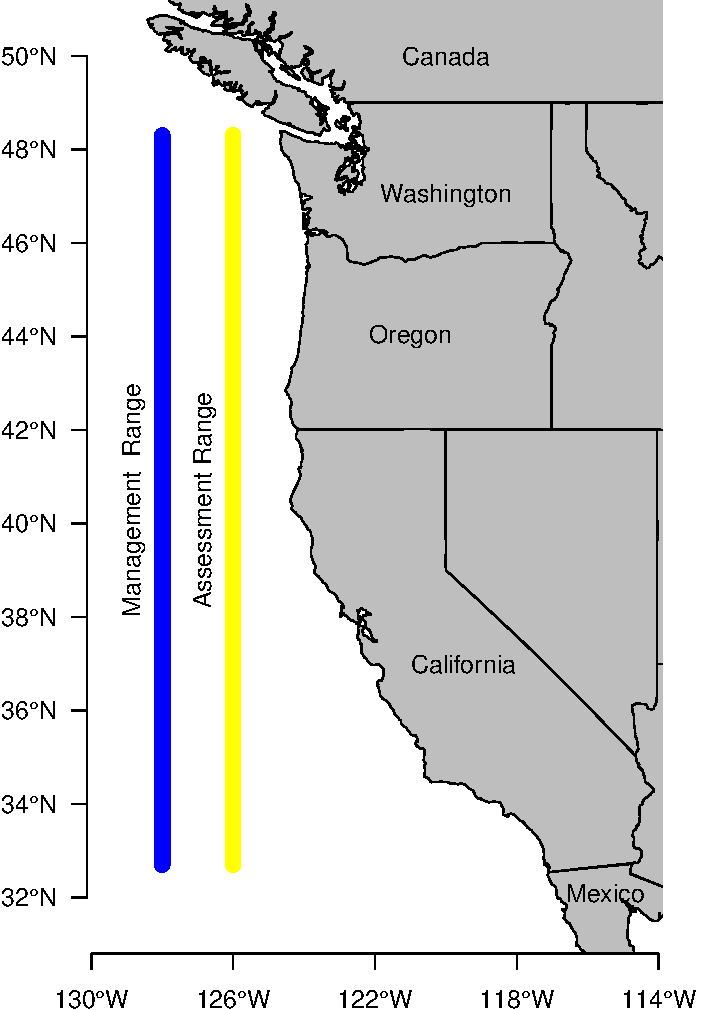
\includegraphics{SAR_USWC_Rougheye_and_Blackspotted_Rockfishes_skeleton_files/figure-pdf/fig-map-1.pdf}

}

\caption{\label{fig-map}Map of the assessment area.}

\end{figure}%

\begin{figure}[H]

\centering{

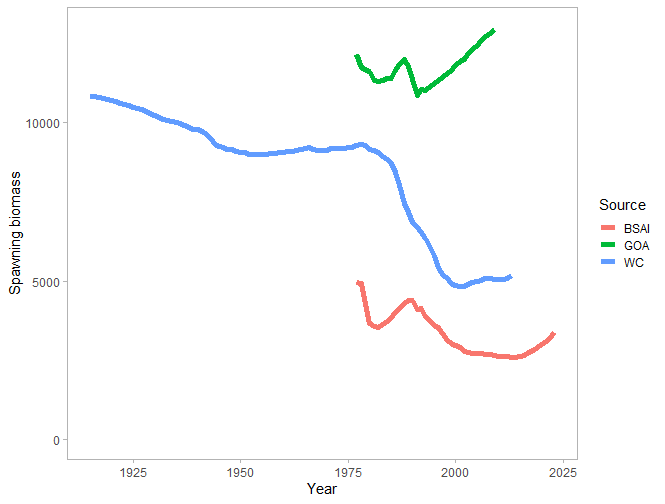
\includegraphics{plots_4_doc/SB_comps.png}

}

\caption{\label{fig-SO_comp}Estimates of spawning biomass (current
spawning output/unfished spawning output) for the Rougheye/Blackspotted
rockfish complex from the two most recent Alaska (Bering Sea/Aleutian
Islands (BSAI) and Gulf of Alaska (GOA)) and the 2013 U.S. west coast
stock assessment.}

\end{figure}%

\begin{figure}[H]

\centering{

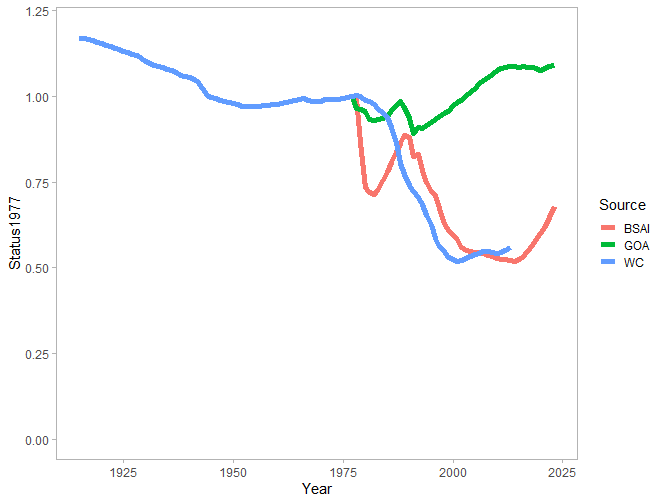
\includegraphics{plots_4_doc/Status_comp.png}

}

\caption{\label{fig-RSS_comp}Estimates of relative stock size (current
spawning output/unfished spawning output) relative to 1977 (the common
year in all stock assessments compared) for the Rougheye/Blackspotted
rockfish complex from the two most recent Alaska (Bering Sea/Aleutian
Islands (BSAI) and Gulf of Alaska (GOA)) and the 2013 U.S. west coast
stock assessment.}

\end{figure}%

\newpage

\subsection{Data}\label{data-1}

\begin{figure}[H]

\centering{

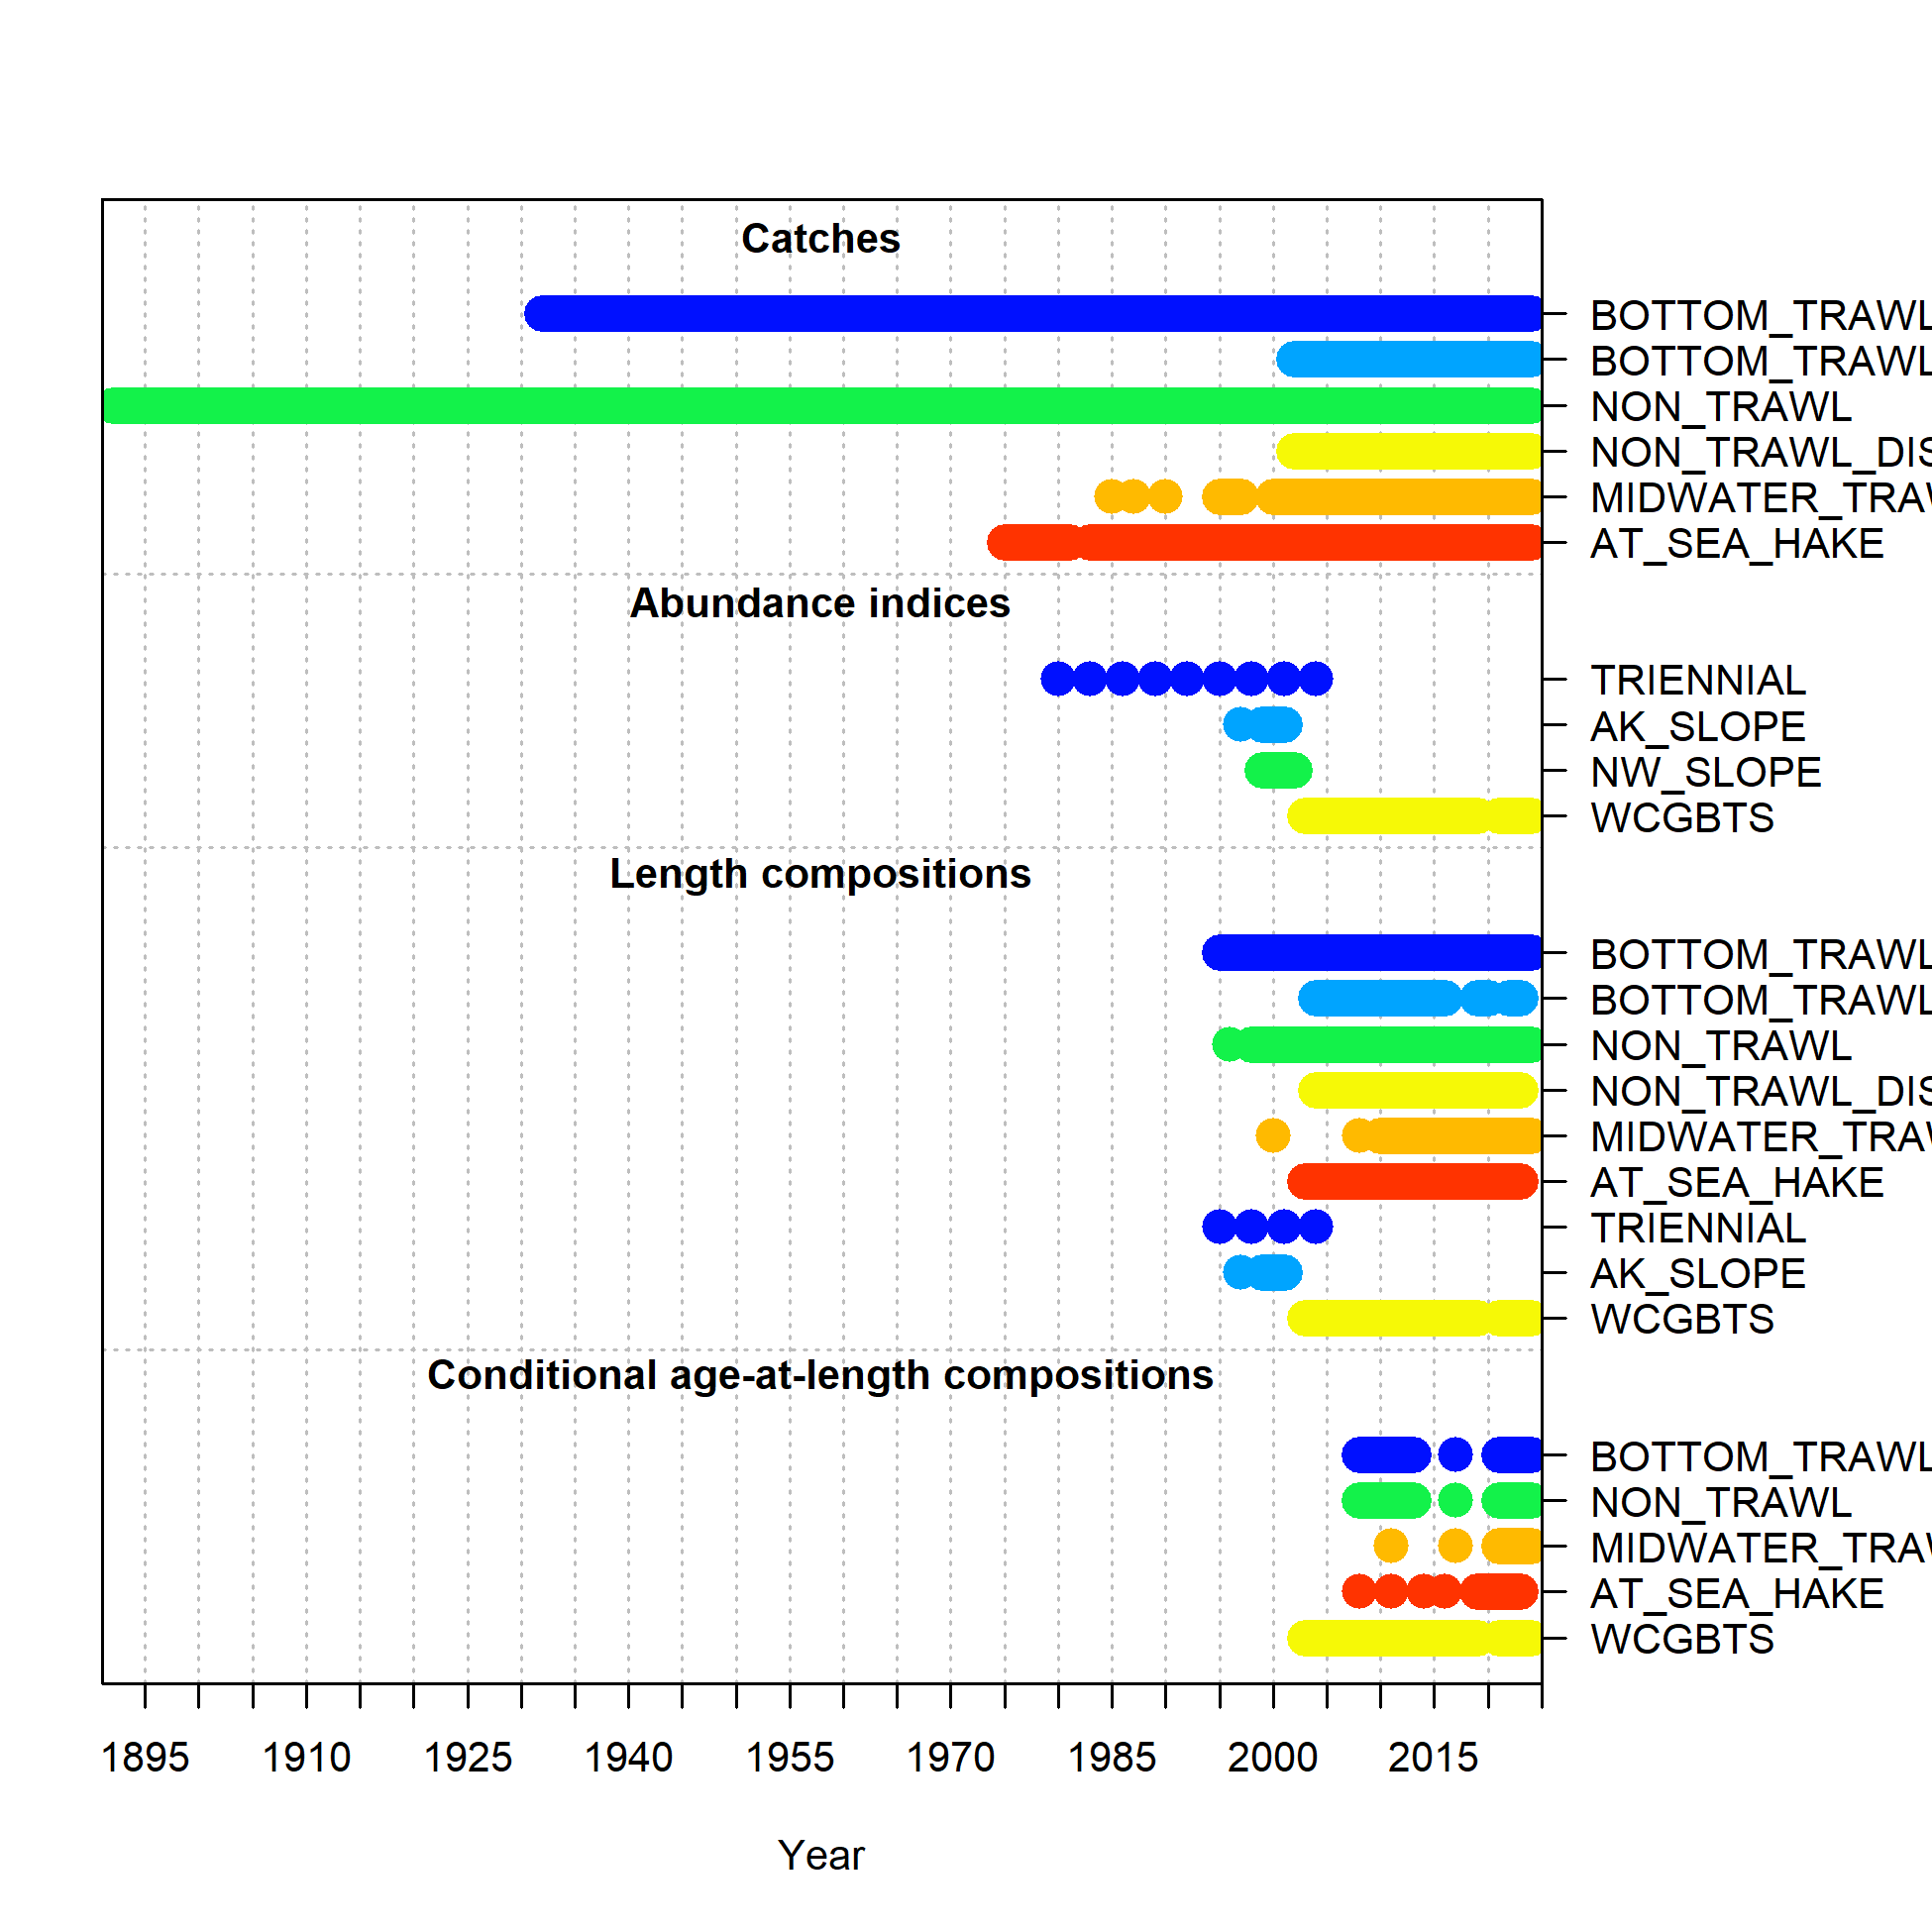
\includegraphics{ref_model/plots/data_plot.png}

}

\caption{\label{fig-data}Data used in the base model.}

\end{figure}%

\begin{figure}[H]

\centering{

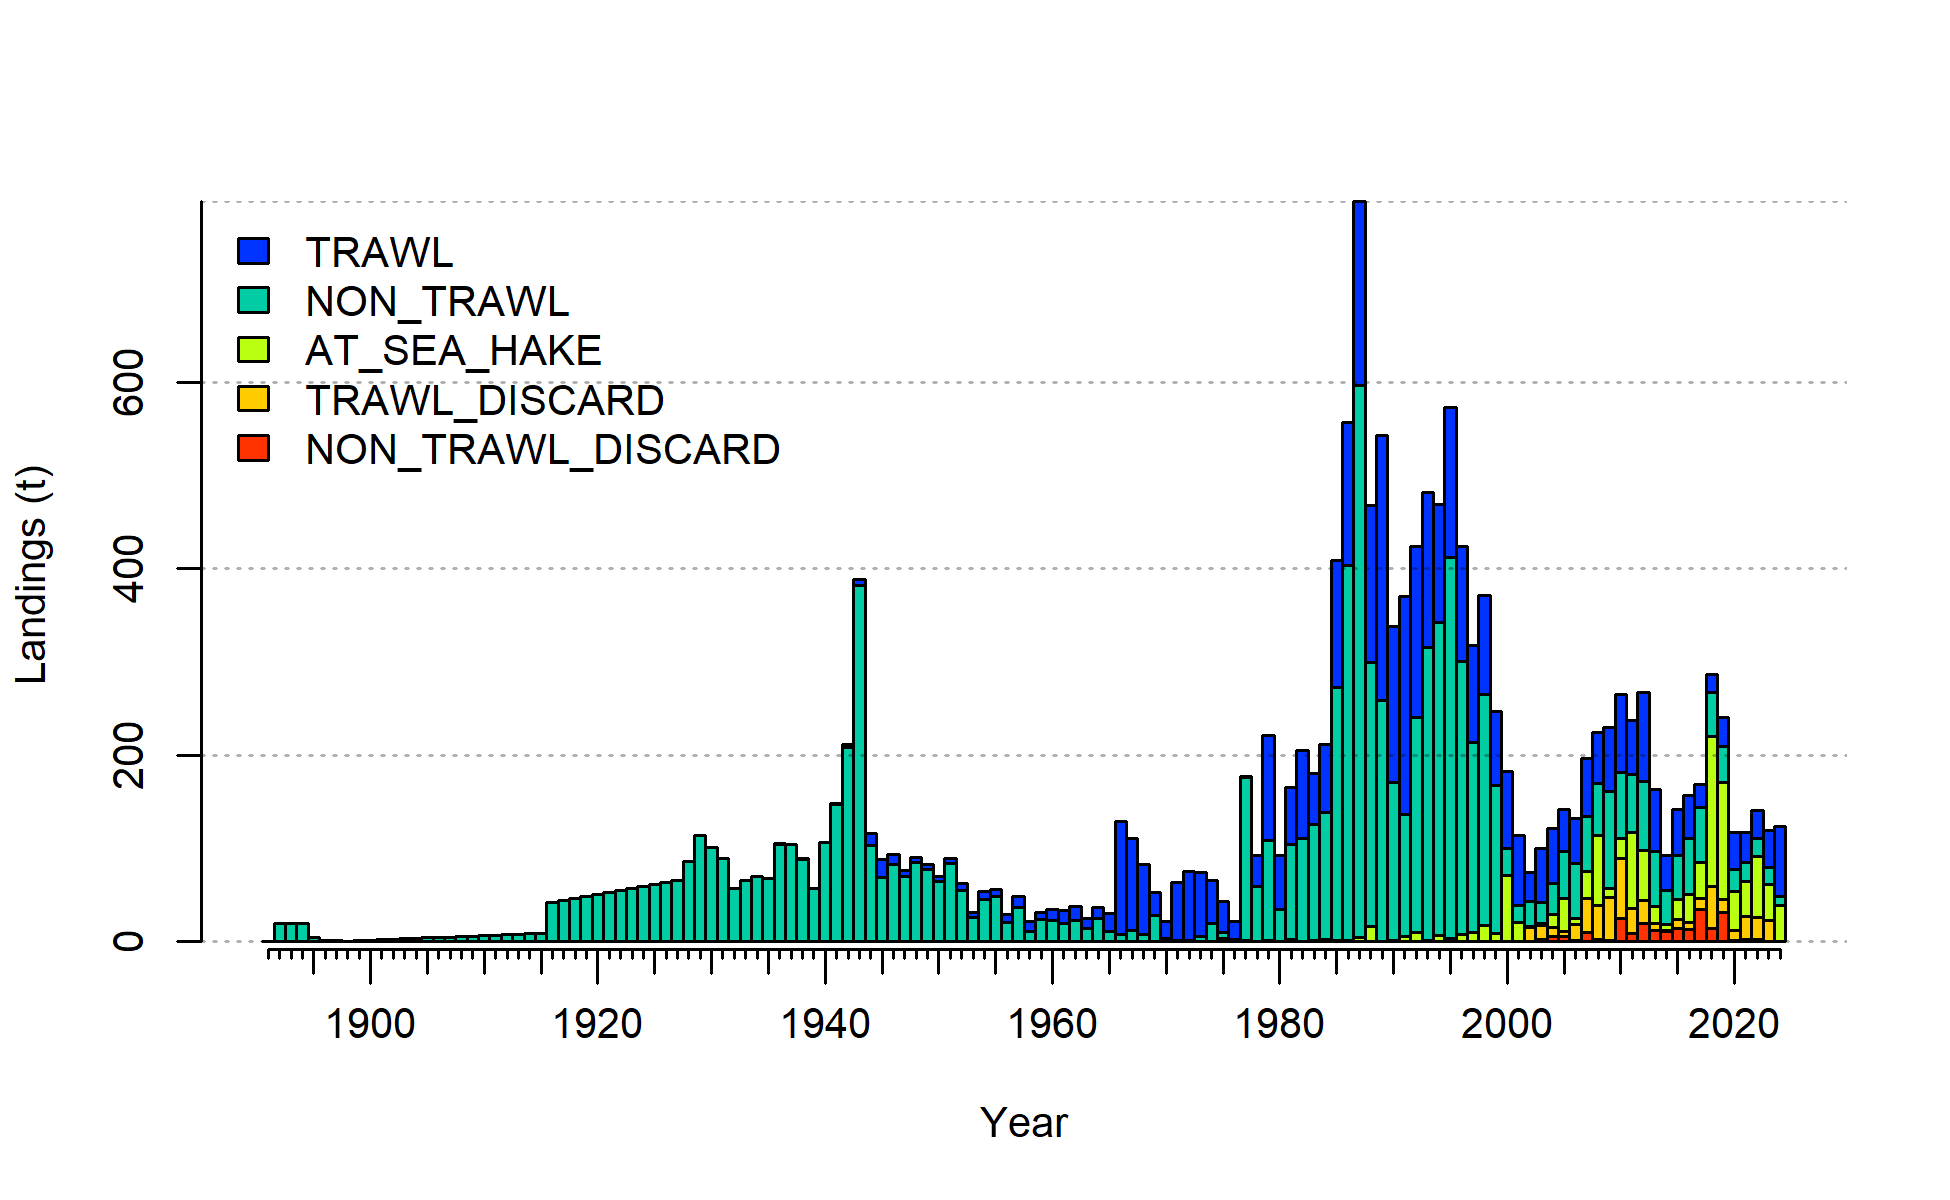
\includegraphics{ref_model/plots/catch2_landings_stacked.png}

}

\caption{\label{fig-landings}Landings by fleet.}

\end{figure}%

\begin{figure}[H]

\centering{

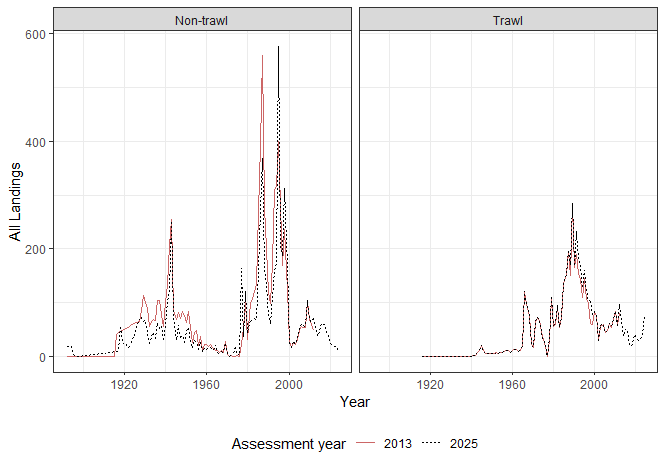
\includegraphics{plots_4_doc/Catch_comp_all.png}

}

\caption{\label{fig-Ct_All}Landings across all states for non-trawl and
trawl fisheries compared between the 2013 assessment and updated
landings for the 2025 stock assessment model.}

\end{figure}%

\begin{figure}[H]

\centering{

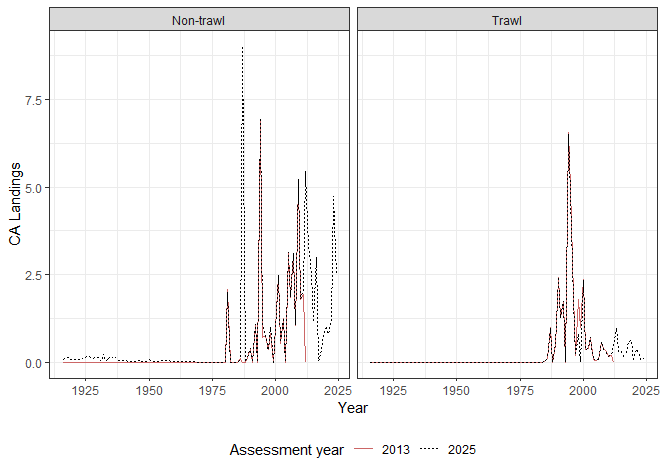
\includegraphics{plots_4_doc/Catch_comp_CA.png}

}

\caption{\label{fig-Ct_CA}California state landings for non-trawl and
trawl fisheries compared between the 2013 assessment and updated
landings for the 2025 stock assessment model.}

\end{figure}%

\begin{figure}[H]

\centering{

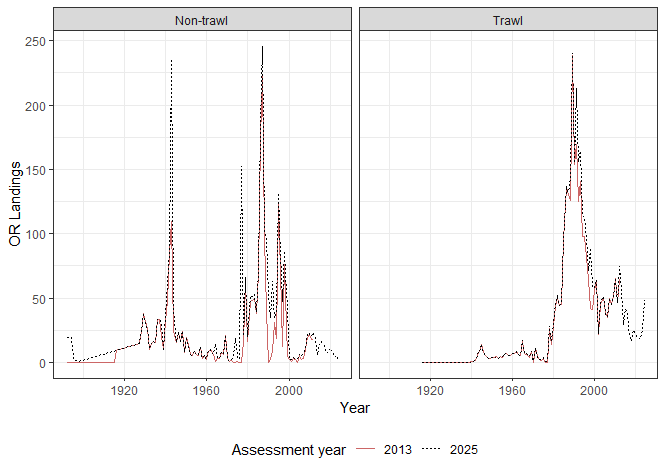
\includegraphics{plots_4_doc/Catch_comp_OR.png}

}

\caption{\label{fig-Ct_OR}Oregon state landings for non-trawl and trawl
fisheries compared between the 2013 assessment and updated landings for
the 2025 stock assessment model.}

\end{figure}%

\begin{figure}[H]

\centering{

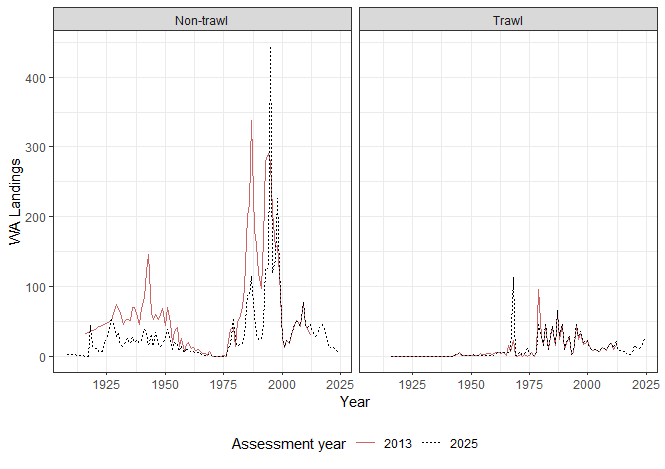
\includegraphics{plots_4_doc/Catch_comp_WA.png}

}

\caption{\label{fig-Ct_WA}WA. Washington state landings for non-trawl
and trawl fisheries compared between the 2013 assessment and updated
landings for the 2025 stock assessment model.}

\end{figure}%

\begin{figure}[H]

\centering{

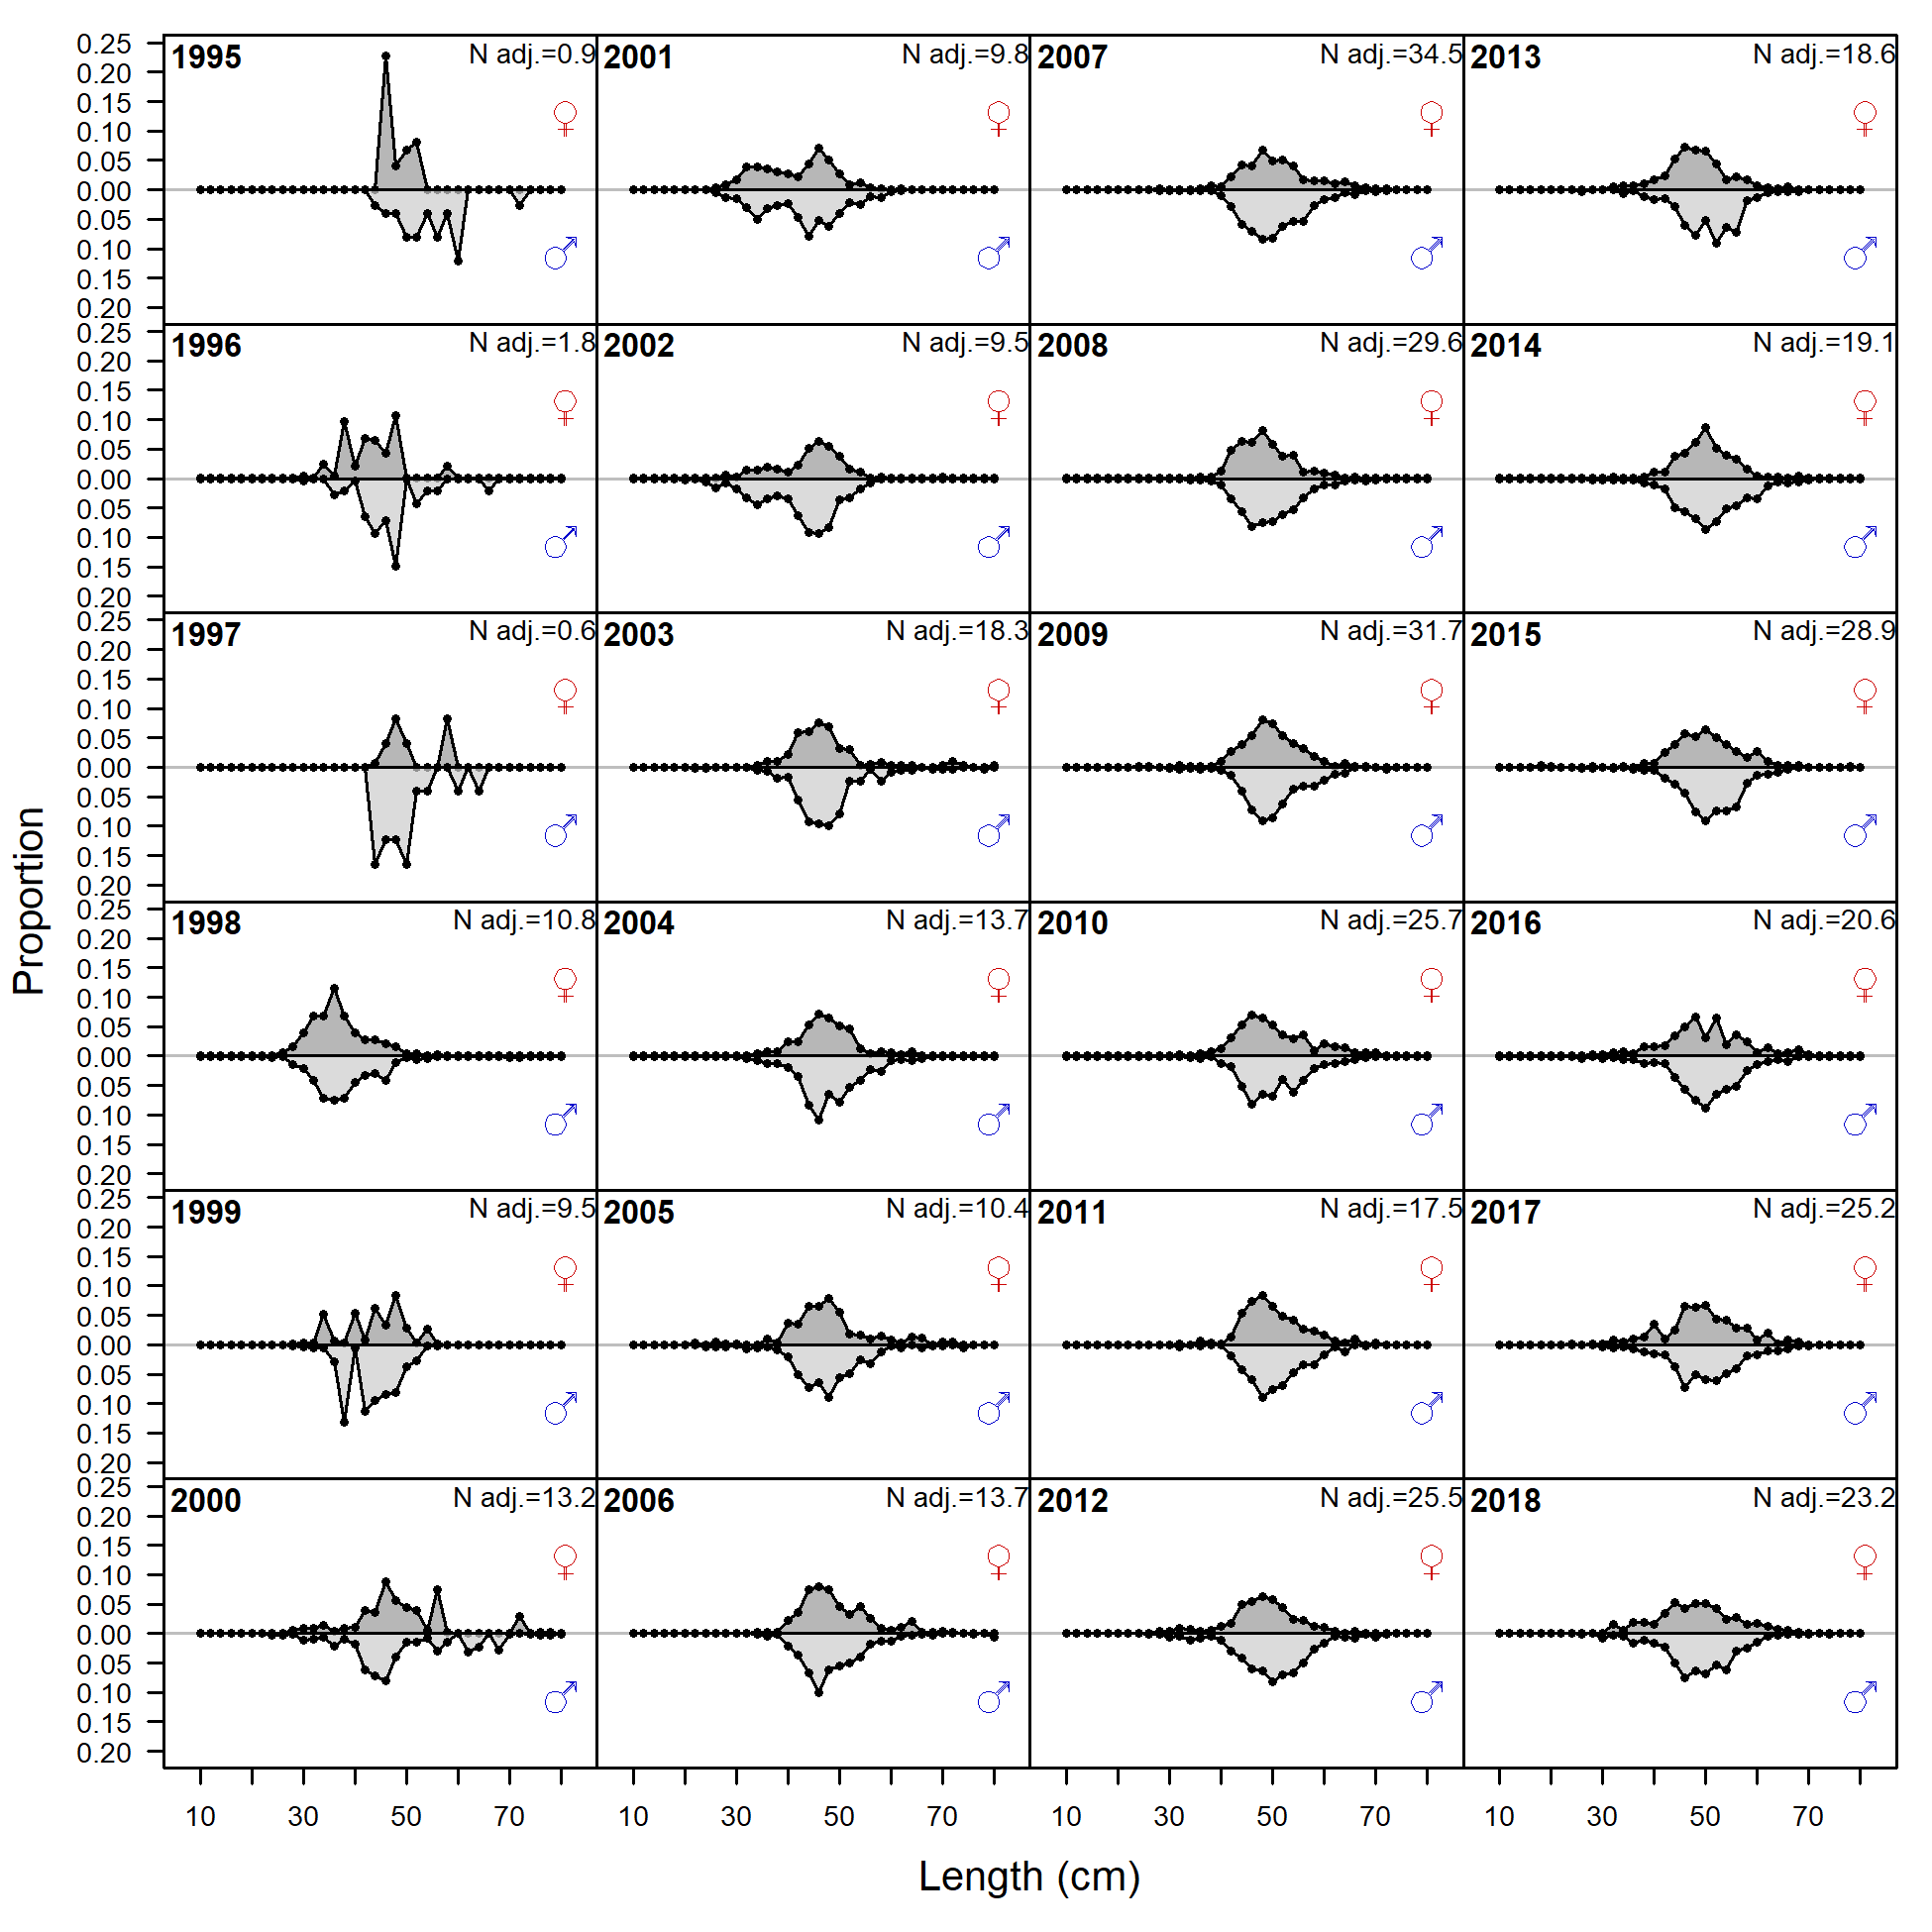
\includegraphics{ref_model/plots/comp_lendat_flt1mkt0_page1.png}

}

\caption{\label{fig-length_flt1_1}Length composition data for bottom
trawl fleet.}

\end{figure}%

\begin{figure}[H]

\centering{

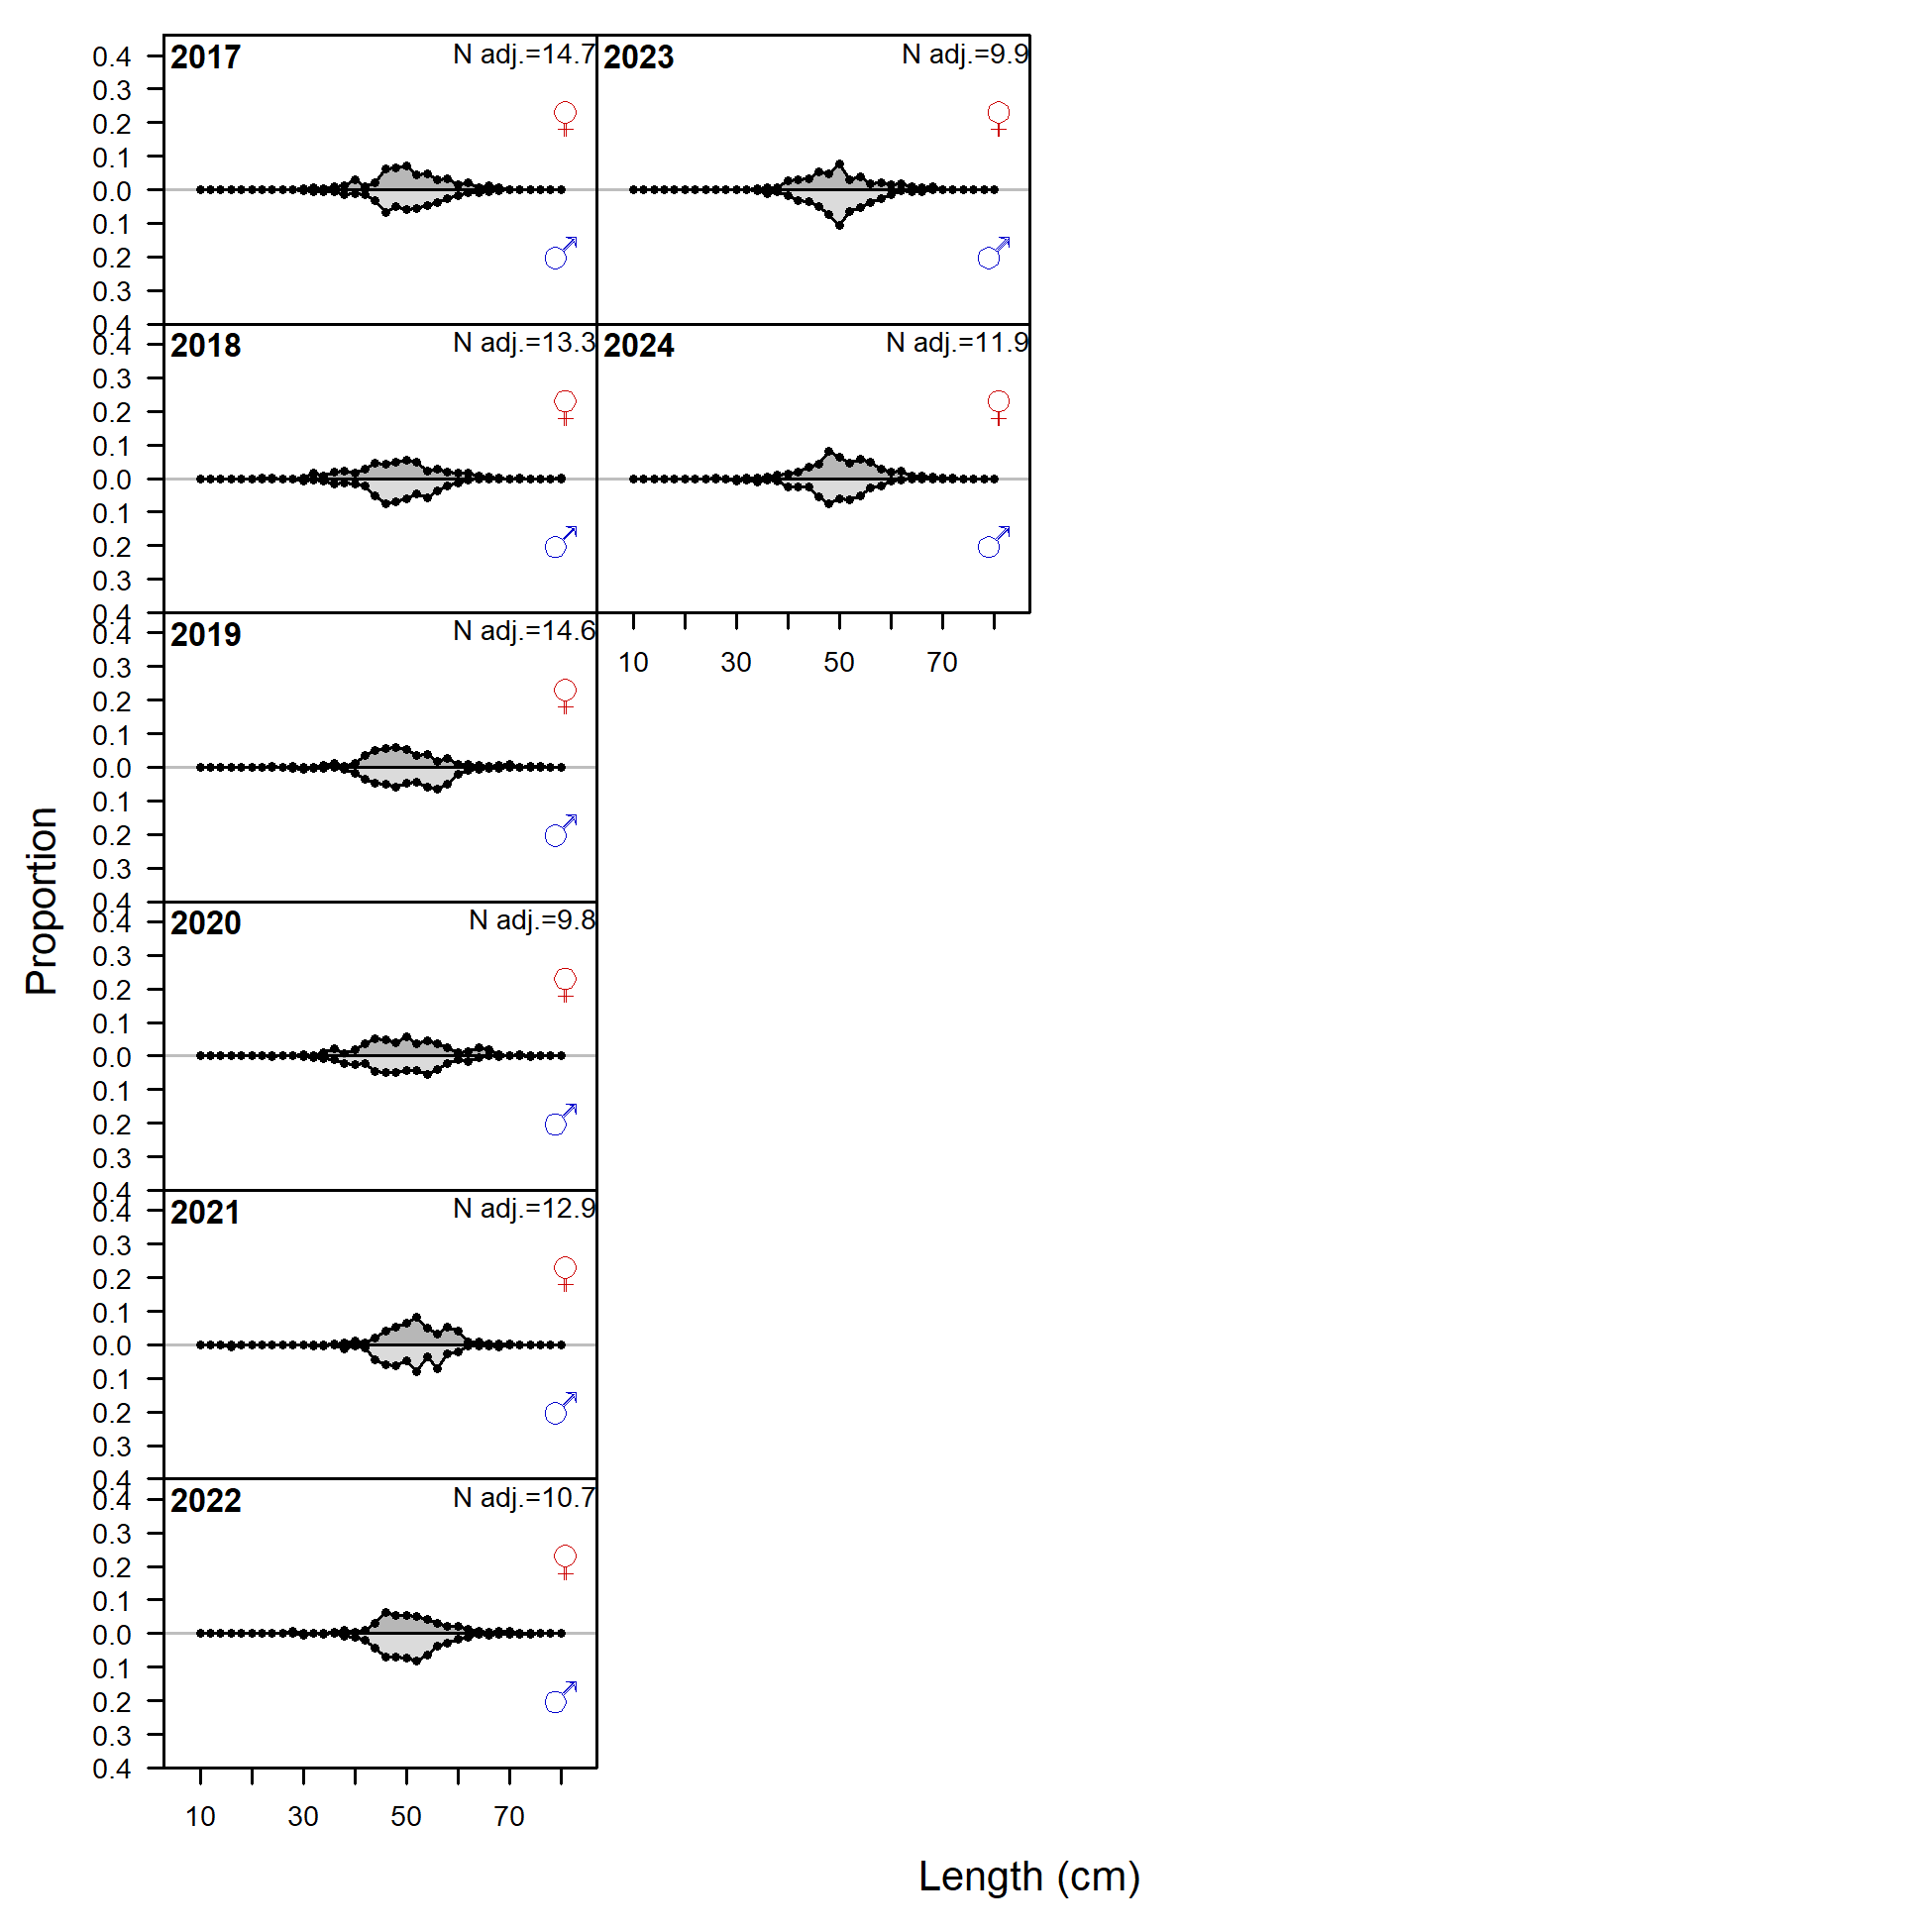
\includegraphics{ref_model/plots/comp_lendat_flt1mkt0_page2.png}

}

\caption{\label{fig-length_flt1_2}Length composition data for bottom
trawl fleet, continued.}

\end{figure}%

\begin{figure}[H]

\centering{

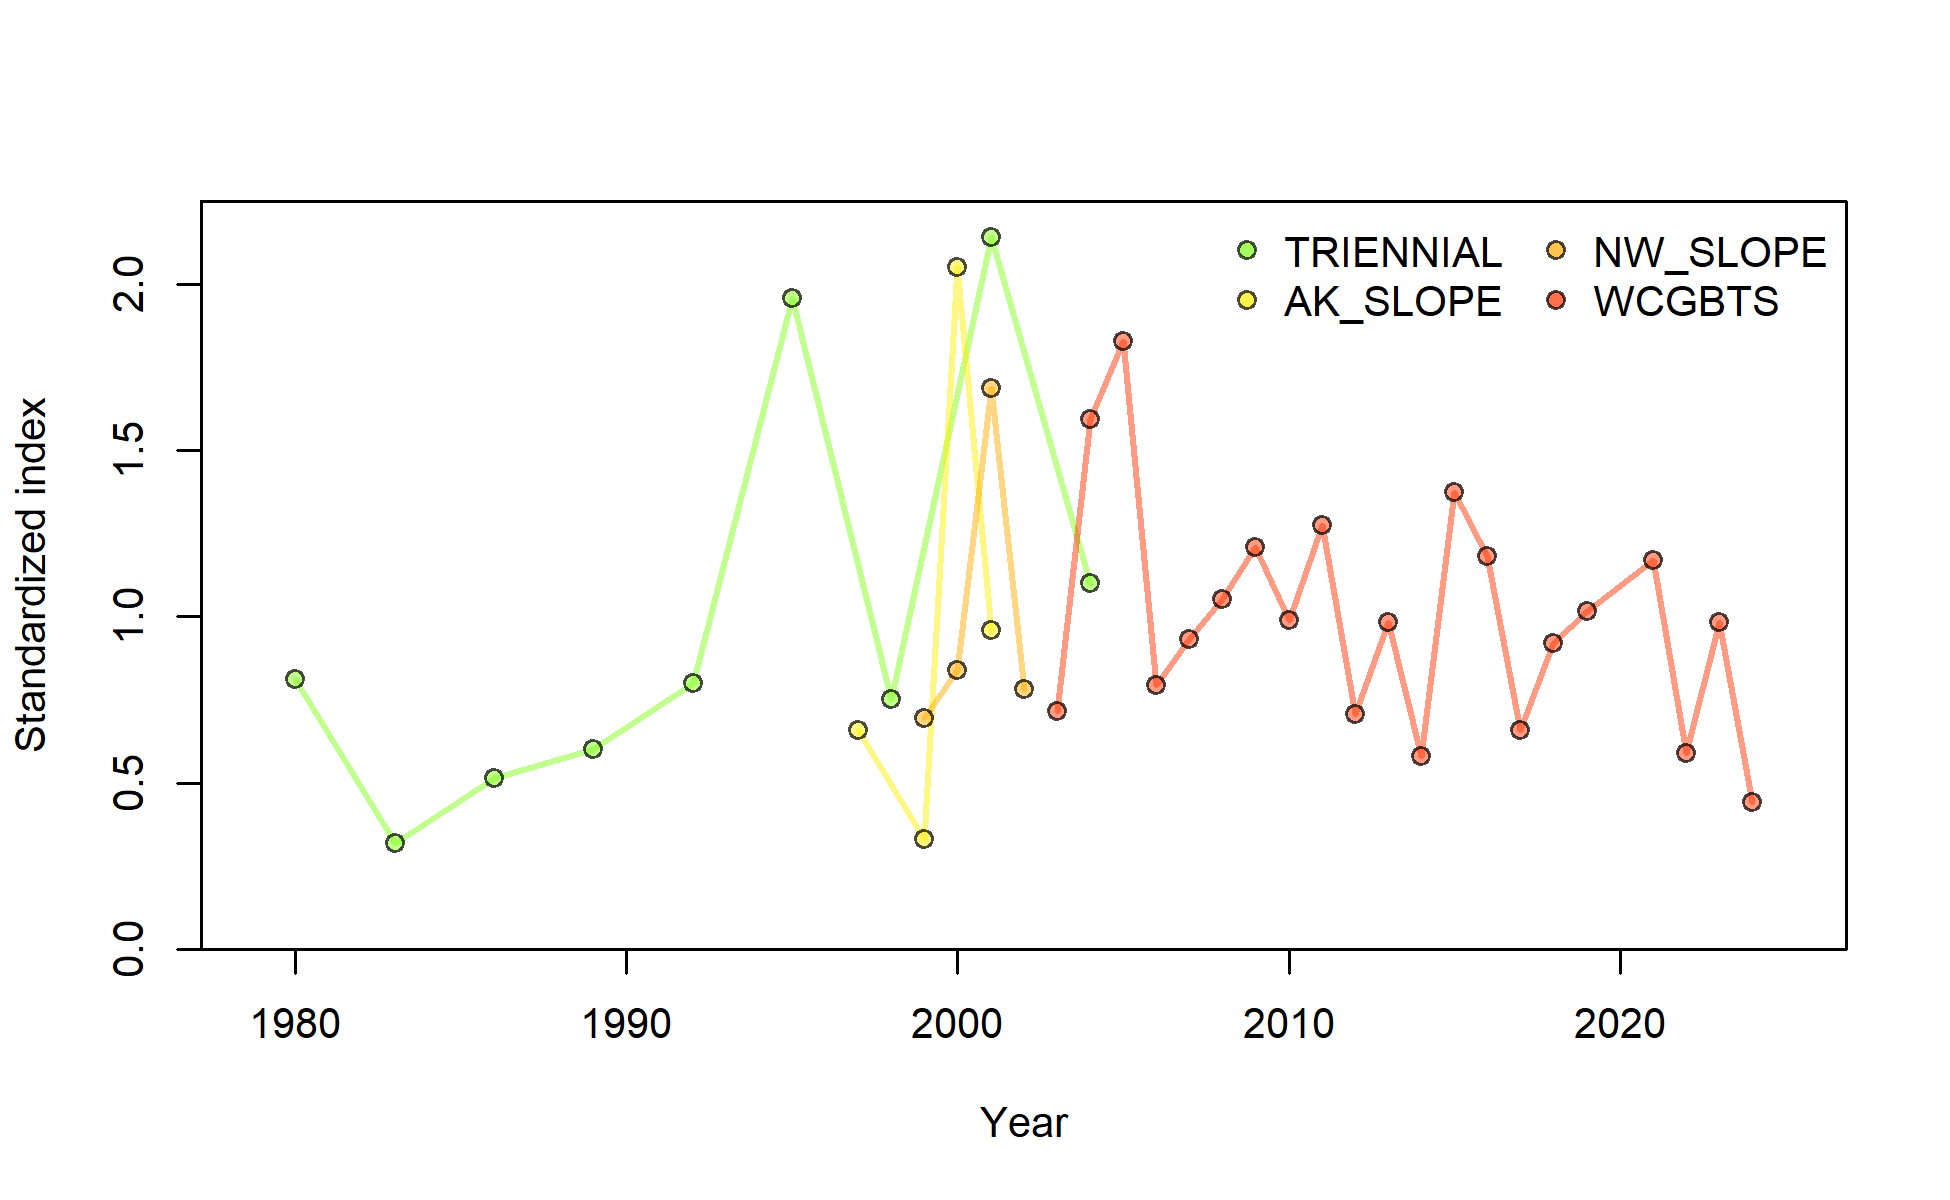
\includegraphics{ref_model/plots/index9_standcpueall.png}

}

\caption{\label{fig-All_indices}Standardized indices.}

\end{figure}%

\begin{figure}[H]

\centering{

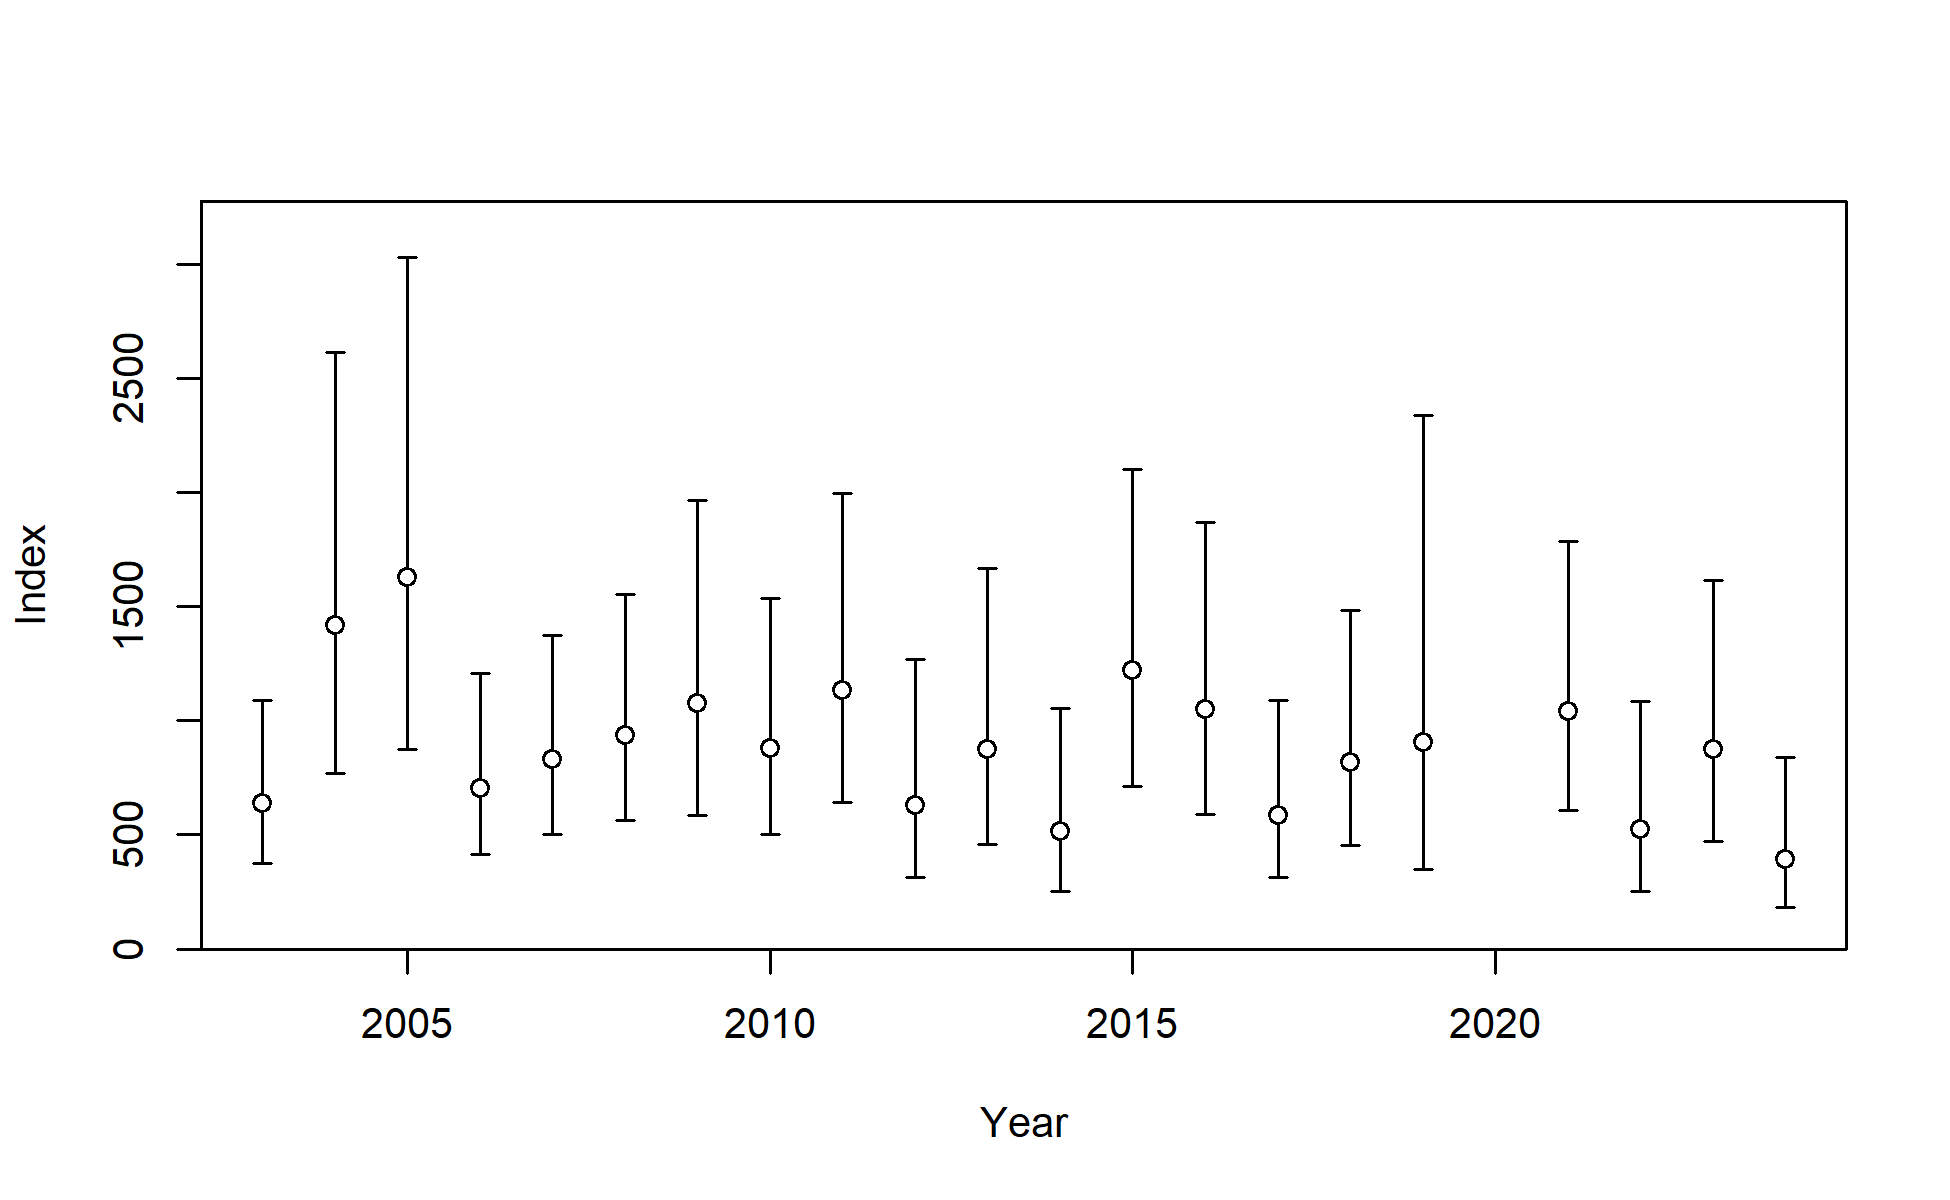
\includegraphics{ref_model/plots/index1_cpuedata_WCGBTS.png}

}

\caption{\label{fig-WCGBTS_index}WCGBTS index.}

\end{figure}%

\begin{figure}[H]

\centering{

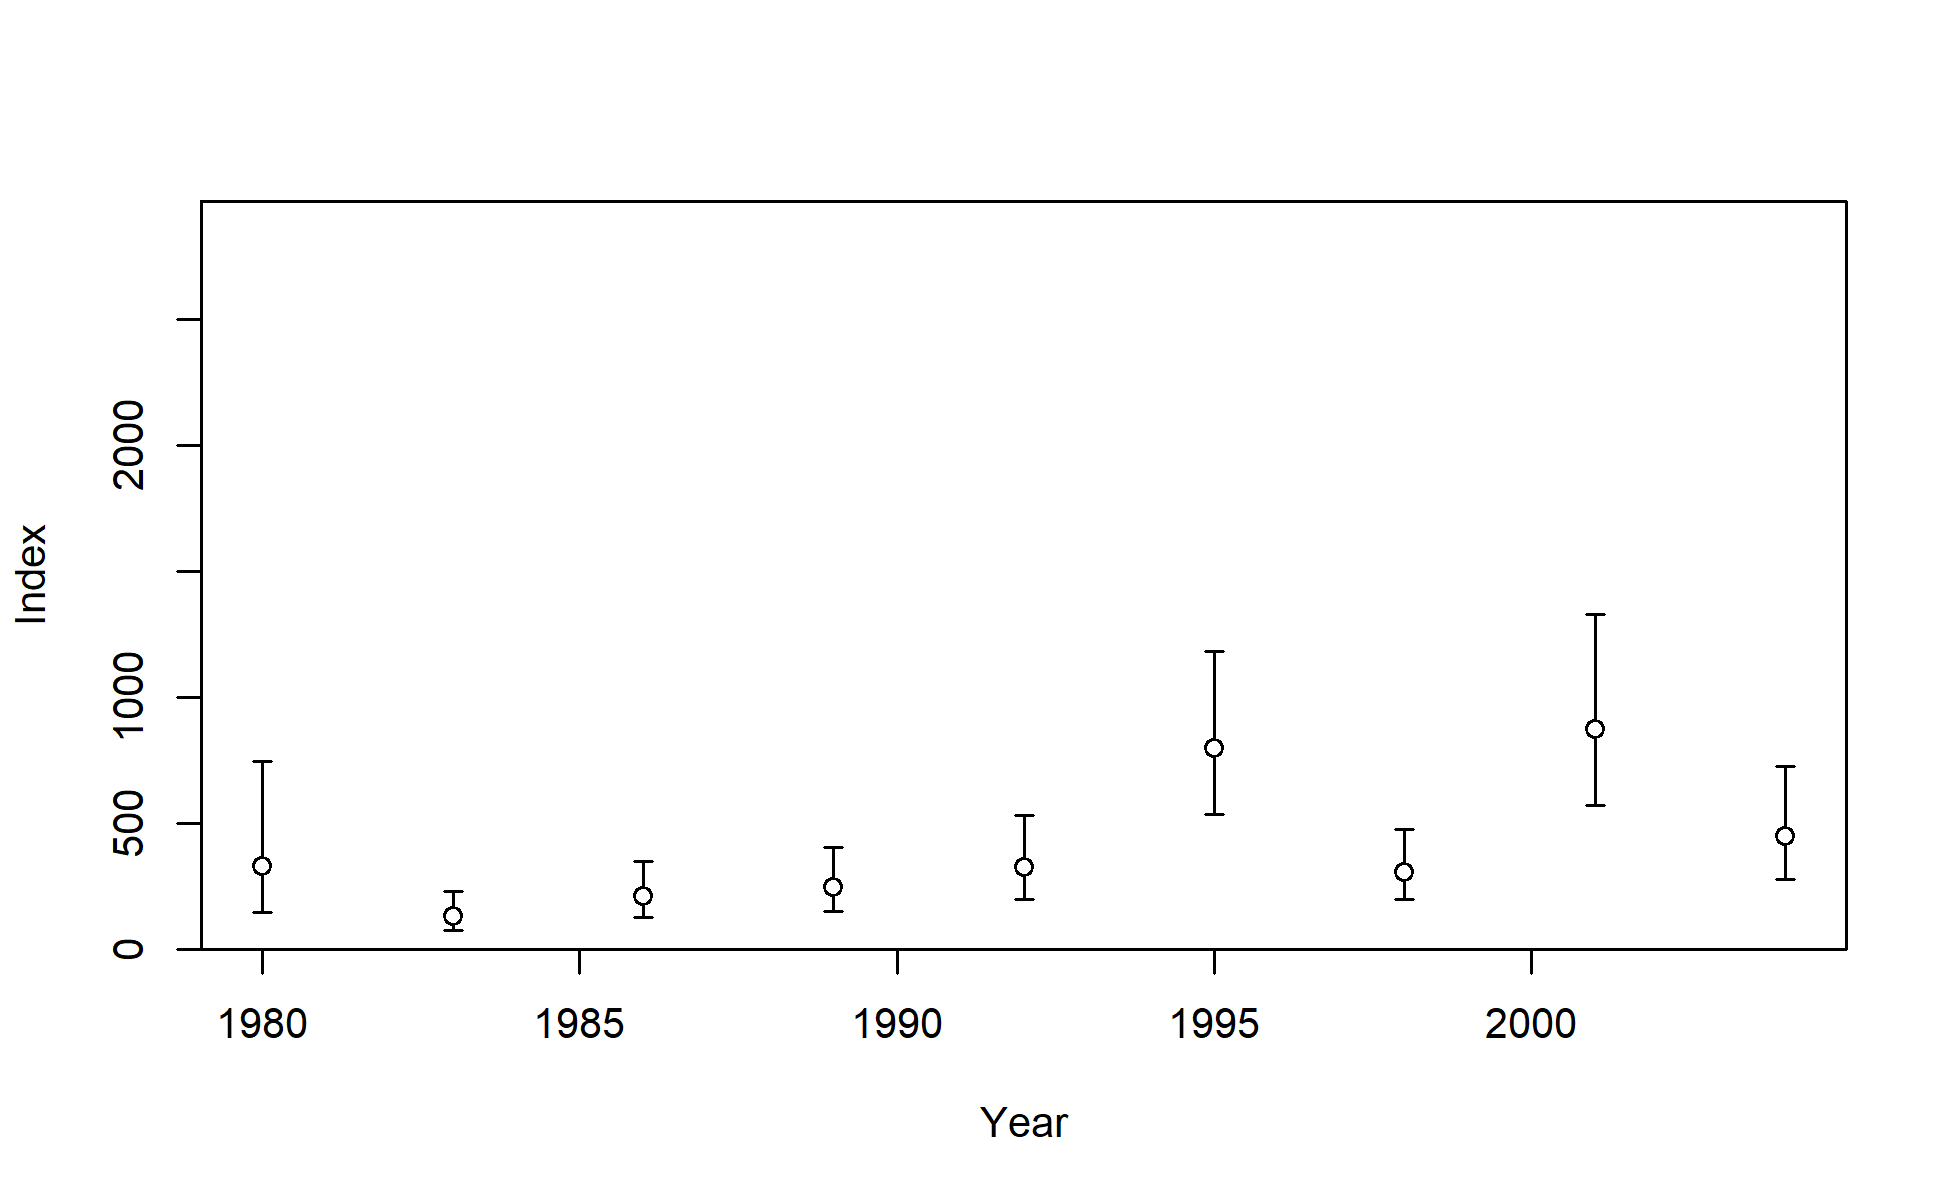
\includegraphics{ref_model/plots/index1_cpuedata_TRIENNIAL.png}

}

\caption{\label{fig-Triennial_index}Triennial Survey index.}

\end{figure}%

\begin{figure}[H]

\centering{

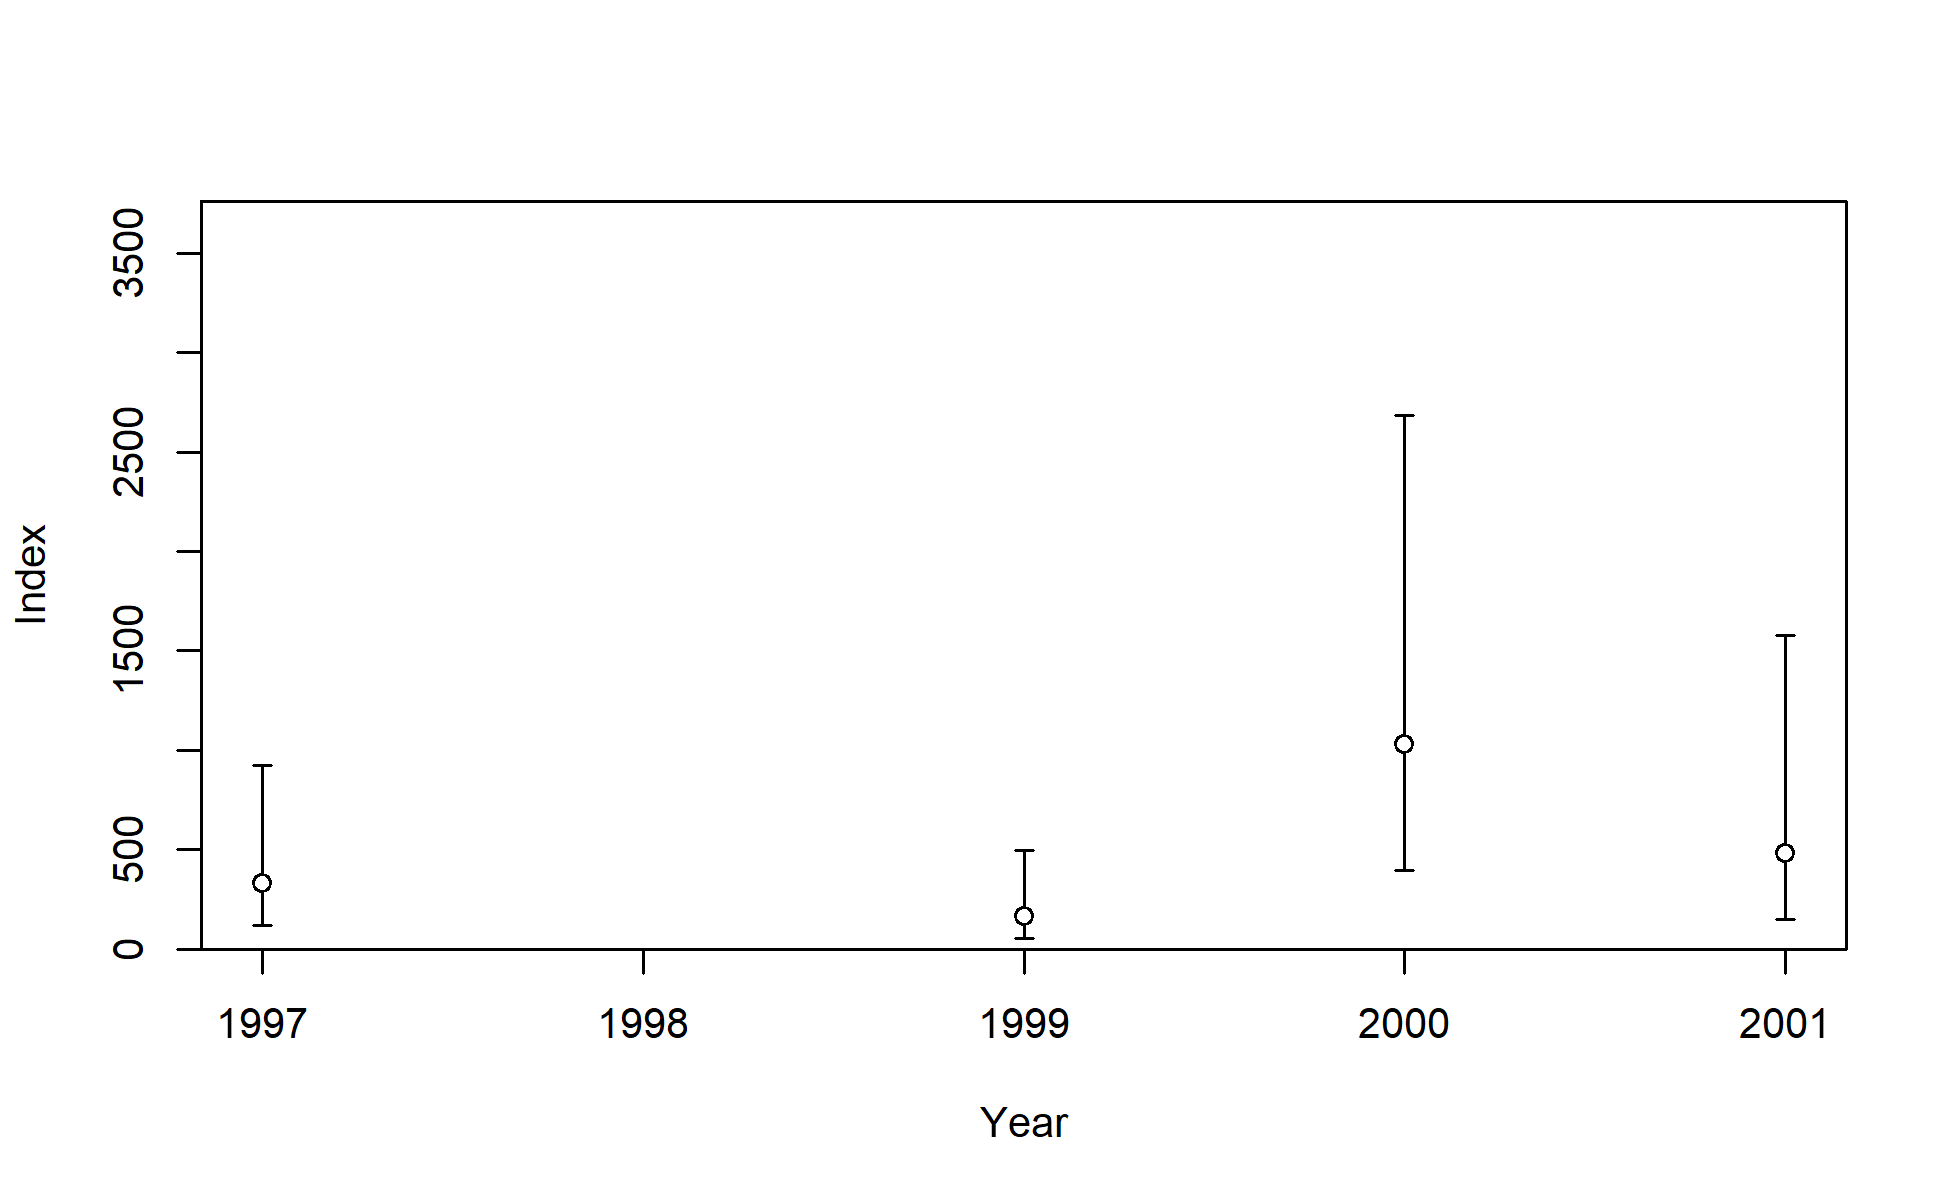
\includegraphics{ref_model/plots/index1_cpuedata_AK_SLOPE.png}

}

\caption{\label{fig-AFSC_Slope_index}AFSC Slope Survey index.}

\end{figure}%

\begin{figure}[H]

\centering{

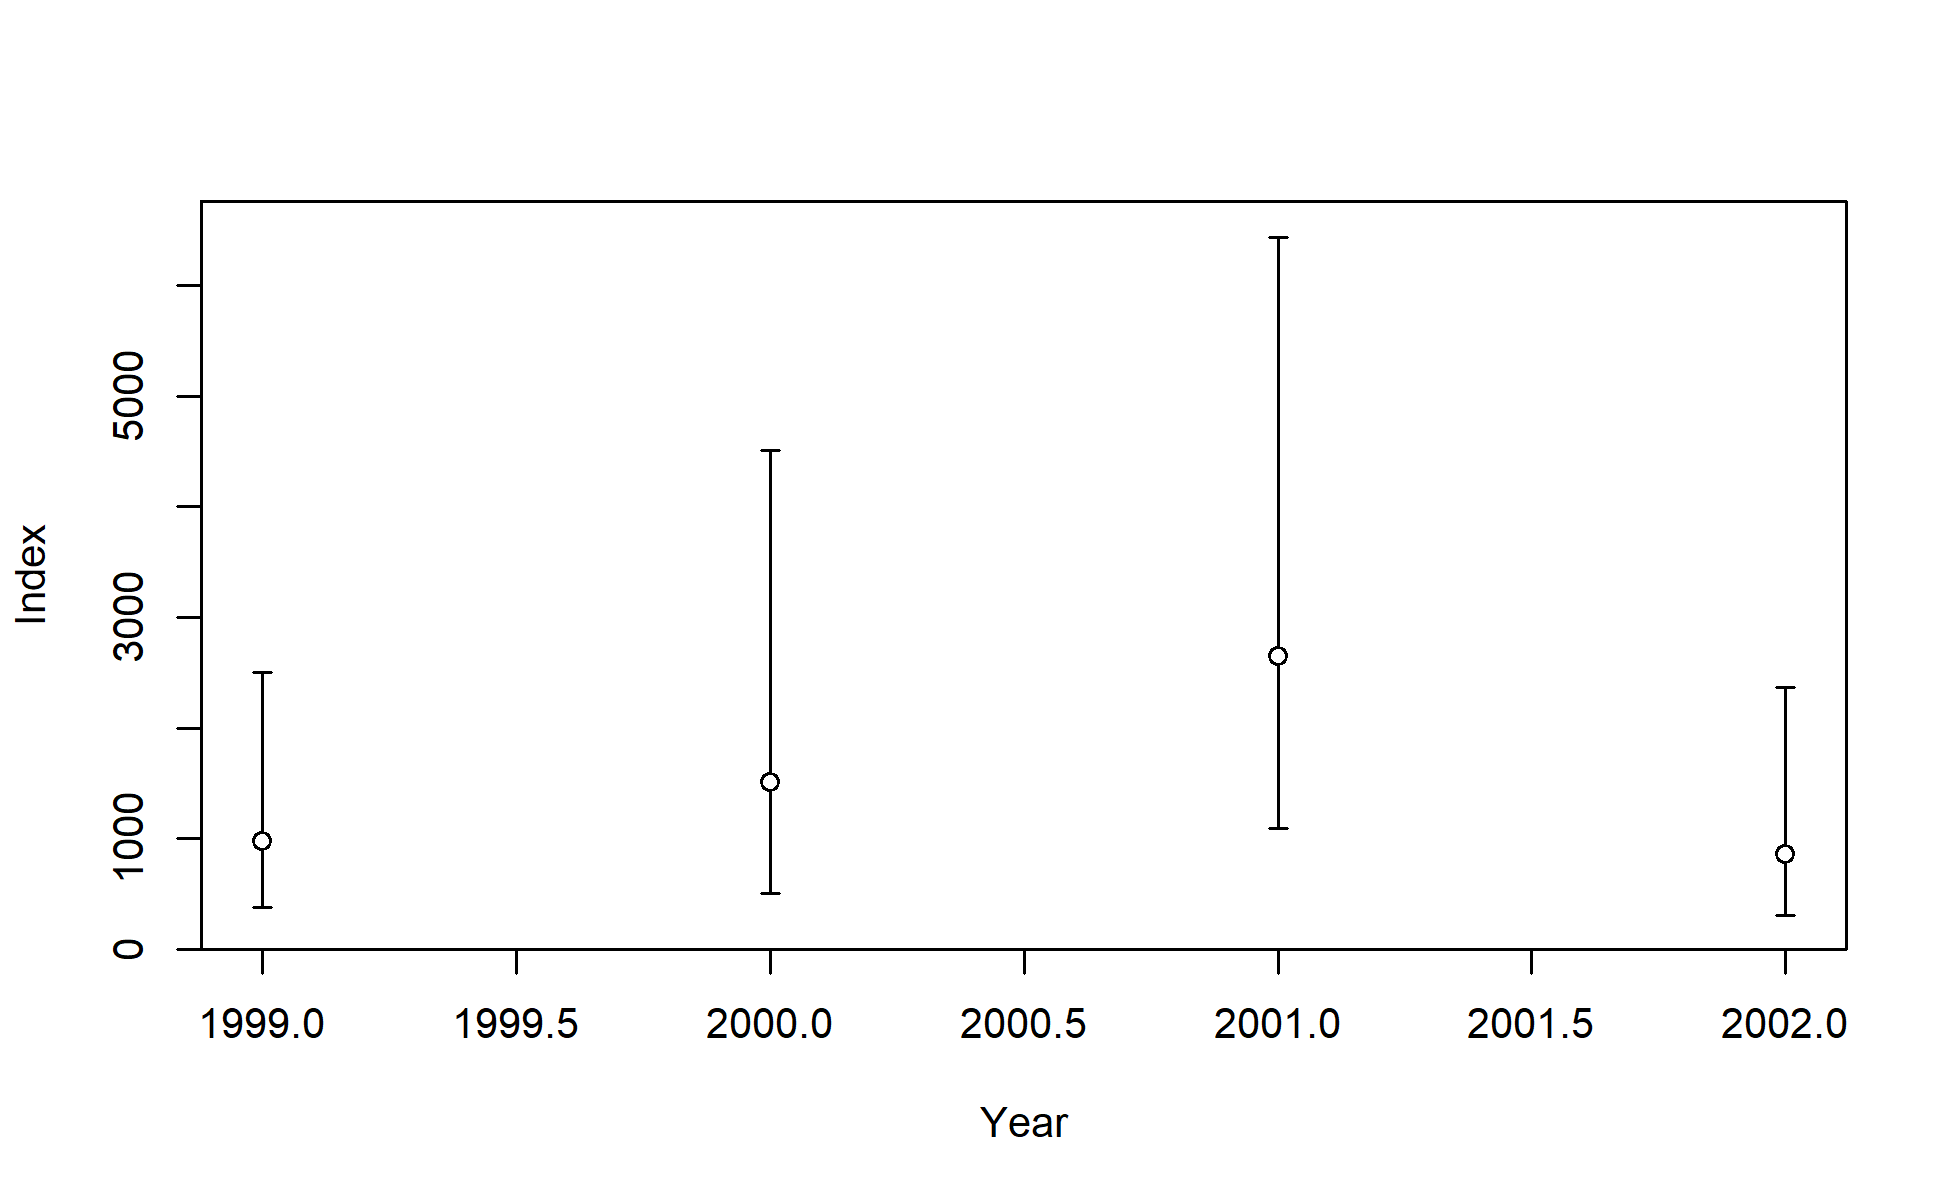
\includegraphics{ref_model/plots/index1_cpuedata_NW_SLOPE.png}

}

\caption{\label{fig-NWFSC_Slope_index}NWFSC Slope Survey index.}

\end{figure}%

\begin{figure}[H]

\centering{

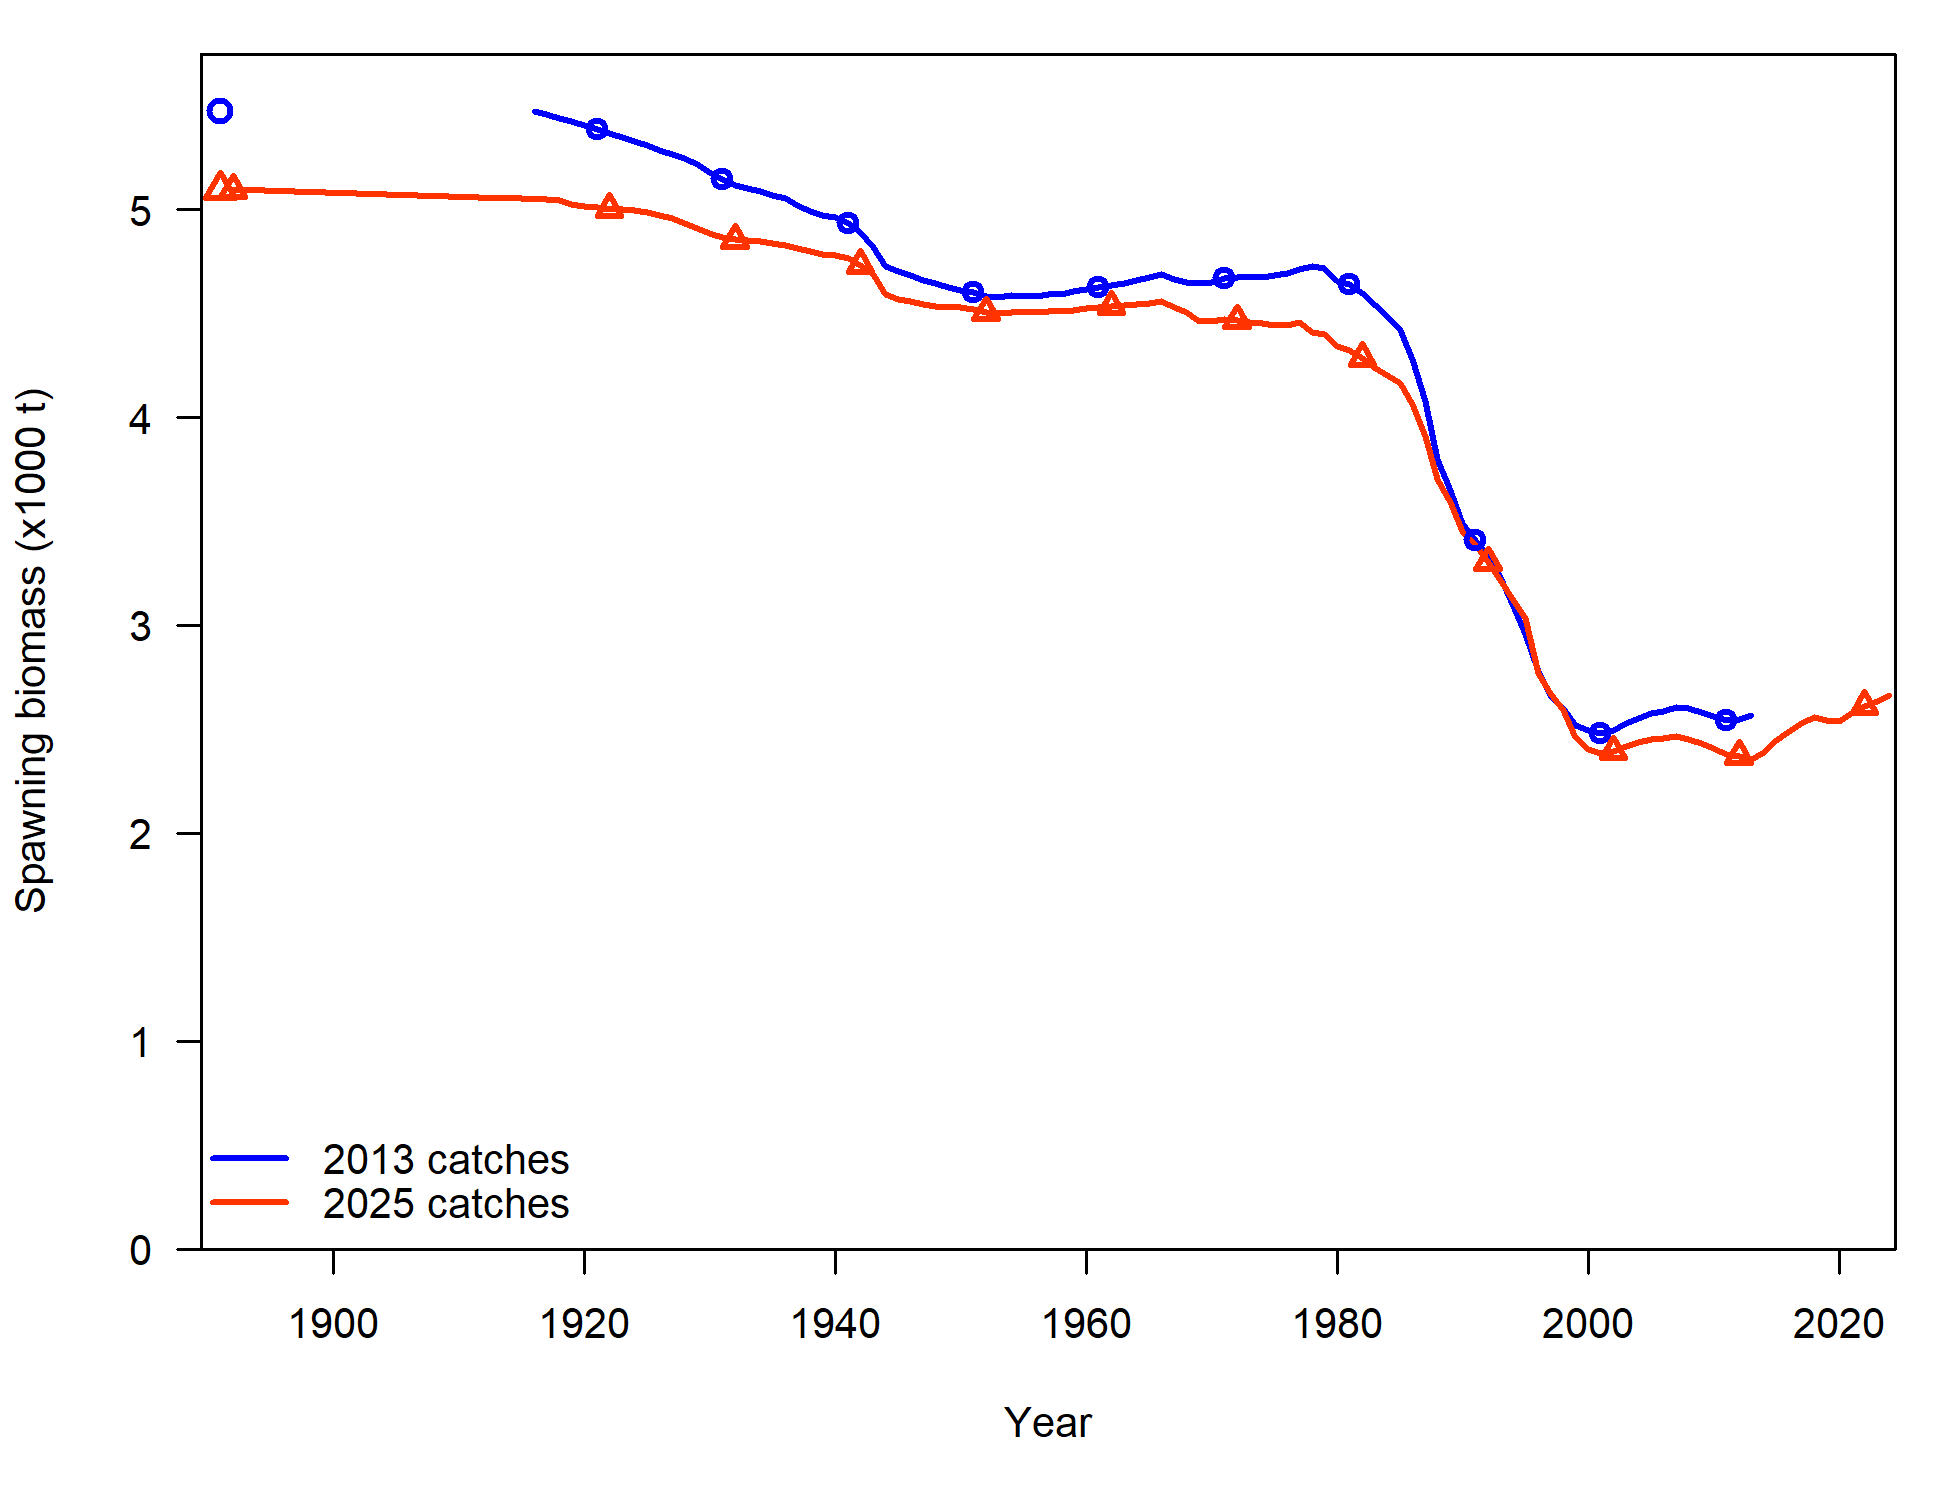
\includegraphics{plots_4_doc/compare1_spawnbio_updatedCt.png}

}

\caption{\label{fig-Ct_compsSO}Comparison of spawning output using
updated catches vs using catches from the 2013 Rougheye/Blackspotted
Rockfishes assessment.}

\end{figure}%

\begin{figure}[H]

\centering{

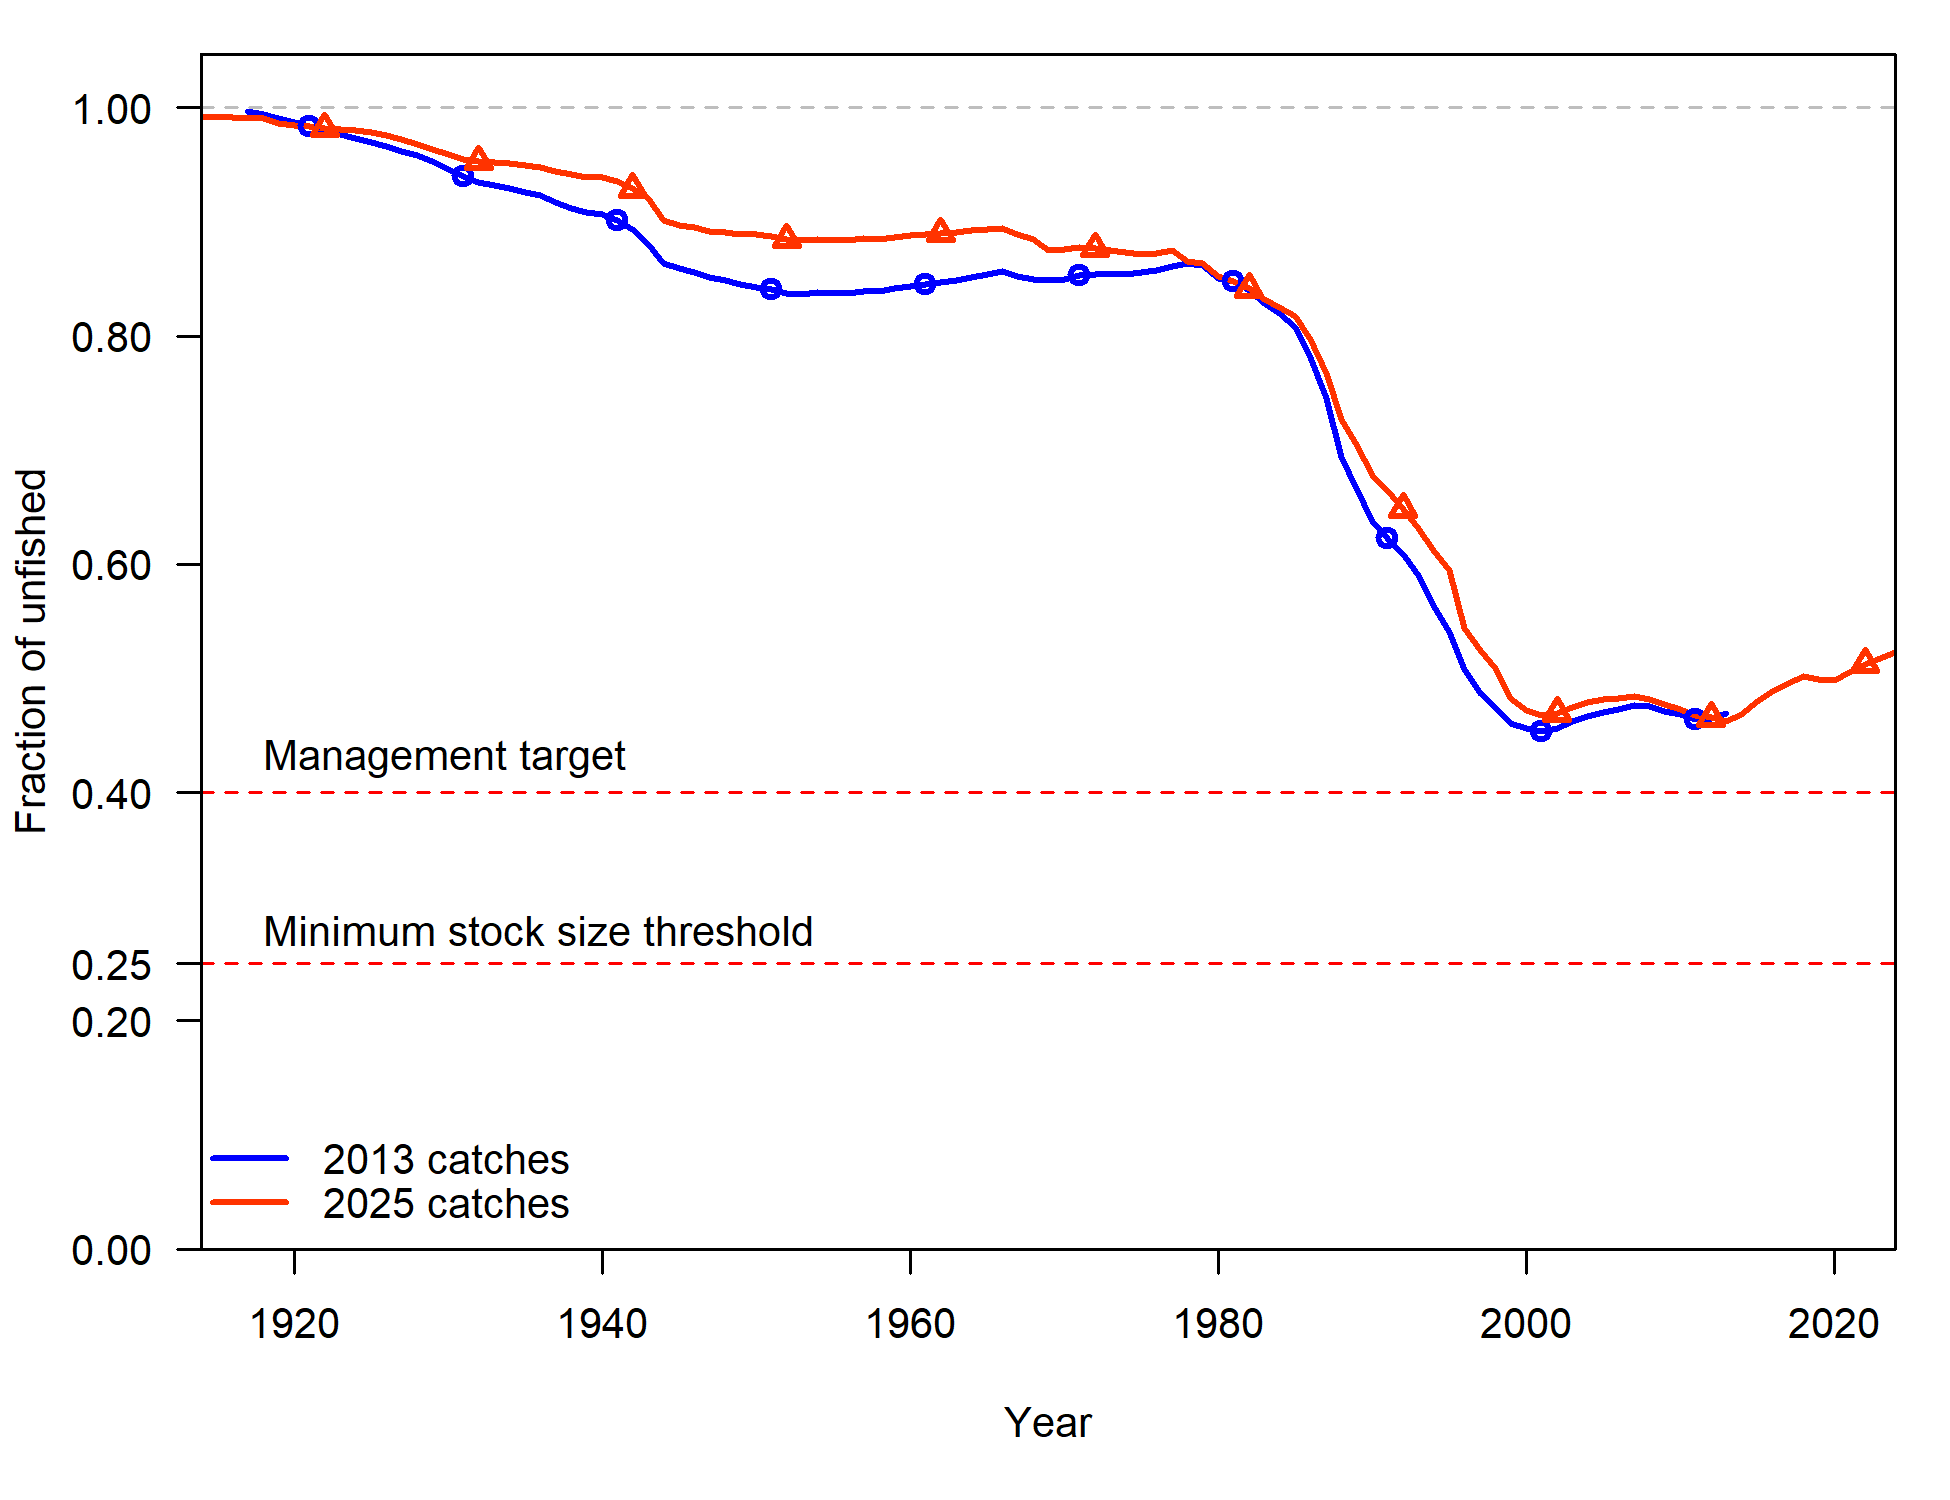
\includegraphics{plots_4_doc/compare3_Bratio_updatedCt.png}

}

\caption{\label{fig-Ct_compsRSS}Comparison of relative spawning output
using updated catches vs using catches from the 2013
Rougheye/Blackspotted Rockfishes assessment.}

\end{figure}%

\newpage

\subsection{Biology}\label{biology}

\begin{figure}[H]

\centering{

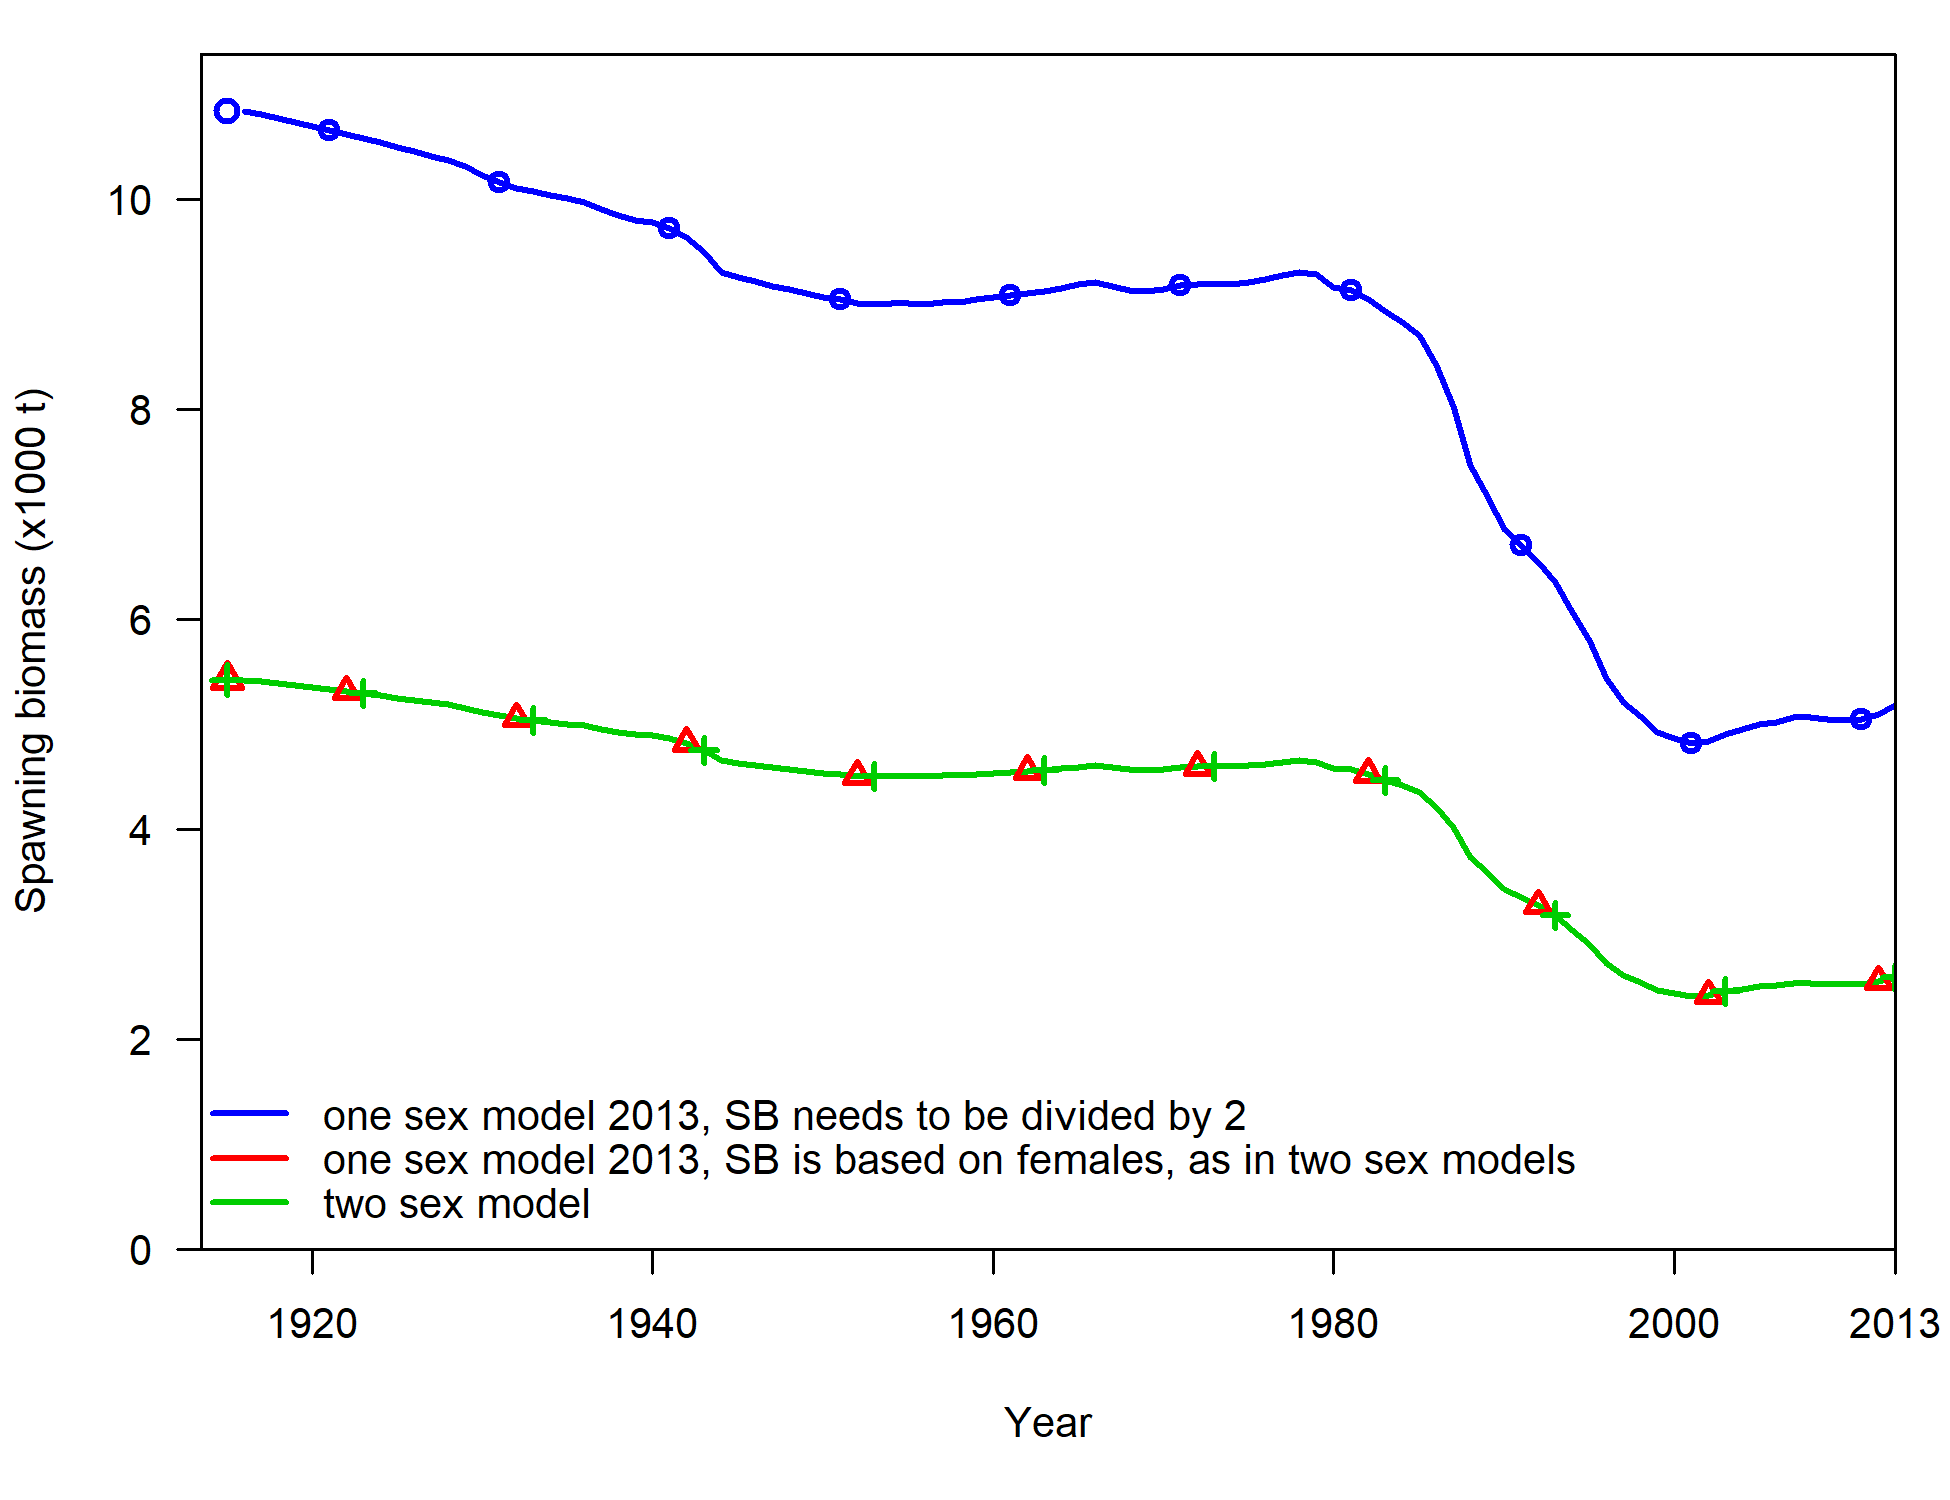
\includegraphics{plots_4_doc/1v2sex_spawnbio.png}

}

\caption{\label{fig-Sex1vs2_SO}Comparison of spawning output using the 1
sex and 2 sexes set to equal values models based on the 2013
Rougheye/Blackspotted Rockfishes assessment data. The 1 sex model has
double the biomass because it includes both females and males.}

\end{figure}%

\begin{figure}[H]

\centering{

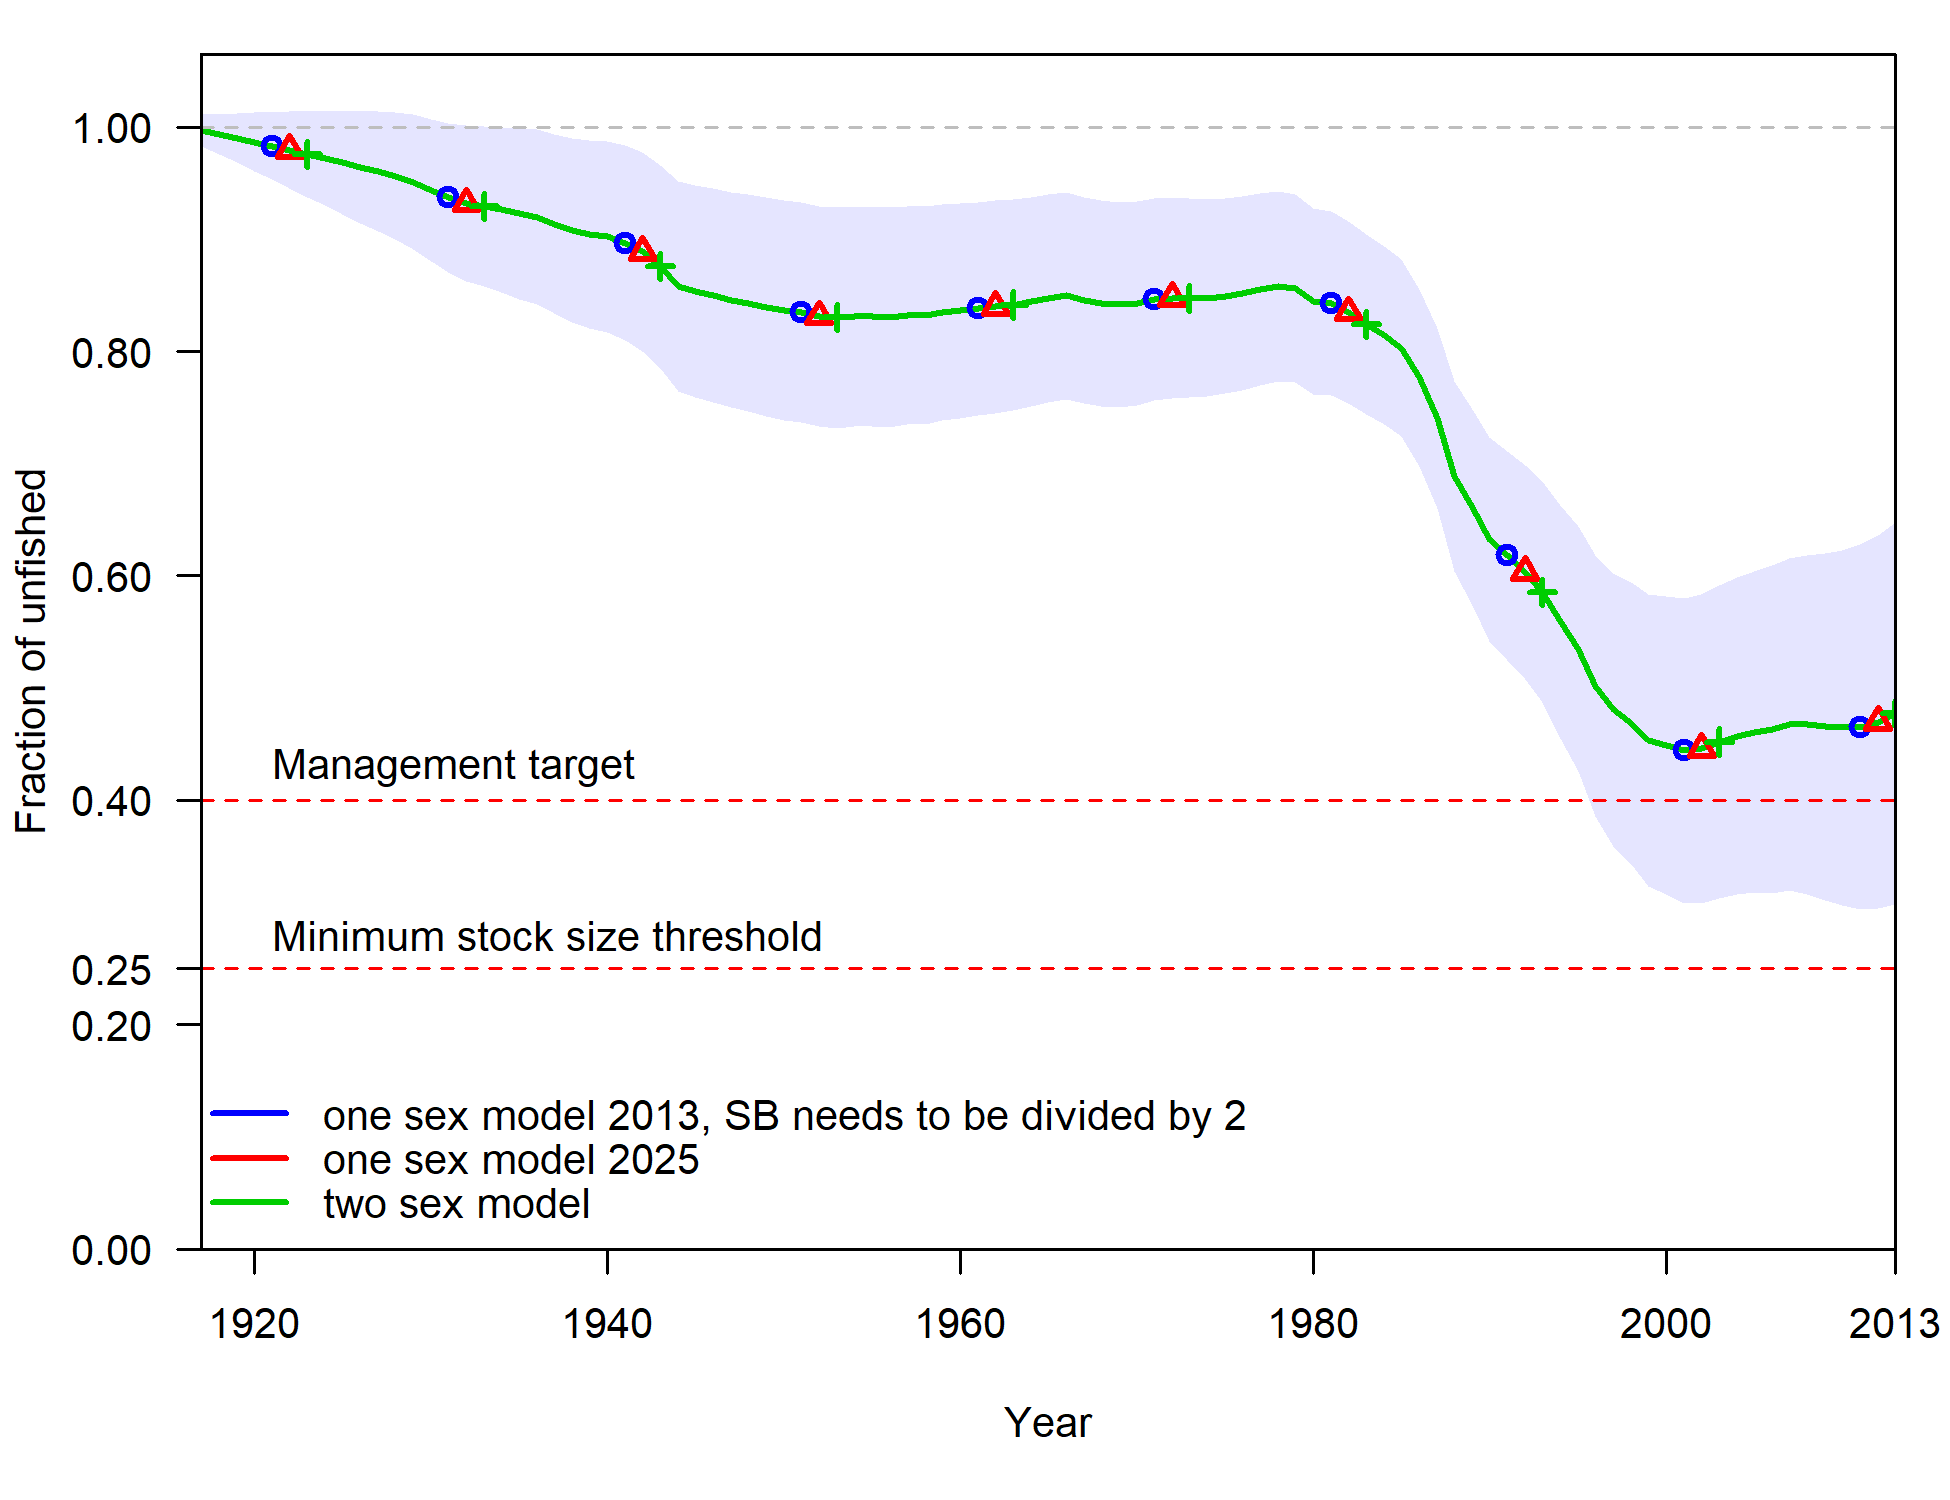
\includegraphics{plots_4_doc/1v2sex_Bratio_uncertainty.png}

}

\caption{\label{fig-Sex1vs2_Bratio}Comparison of spawning output using
the 1 sex and 2 sexes set to equal values models based on the 2013
Rougheye/Blackspotted Rockfishes assessment data.}

\end{figure}%

\begin{figure}[H]

\centering{

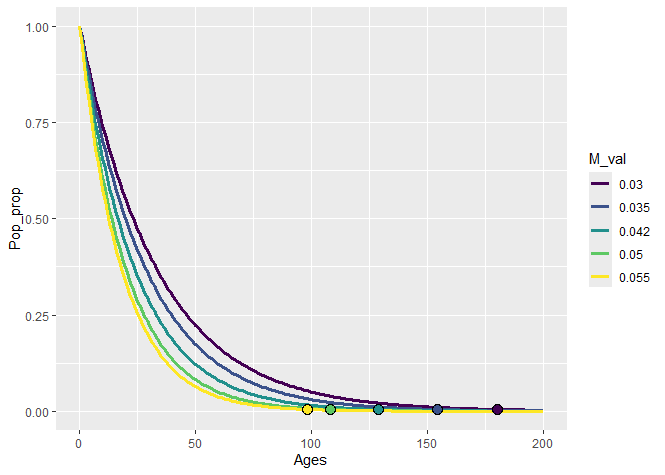
\includegraphics{plots_4_doc/M_values.png}

}

\caption{\label{fig-Mcurves}Natural mortality curves by age in years for
values of natural mortality used in various Rougheye/Blackspotted
Rockfish stock assessments. Dots indicate the range of assumed maximum
ages using the equation from Hamel and Cope 2022.}

\end{figure}%

\begin{figure}[H]

\centering{

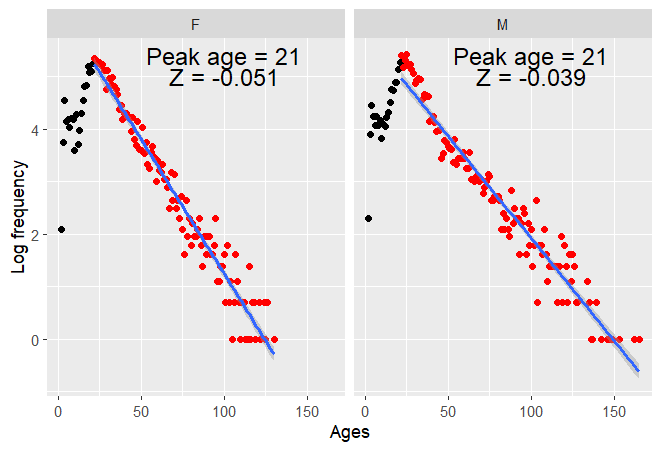
\includegraphics{plots_4_doc/Catch_curve_plot_FM.png}

}

\caption{\label{fig-CC_Z}Catch curve (log abundance by age) analysis on
aggregated ages over all age sources by sex (black points). The peak
selected age was 21 for both sexes, so the linear model was run from age
21 until the oldest age (red points). The slope of the linear model is
equal to the estimate of an aggregate total mortality (Z).}

\end{figure}%

\begin{figure}[H]

\centering{

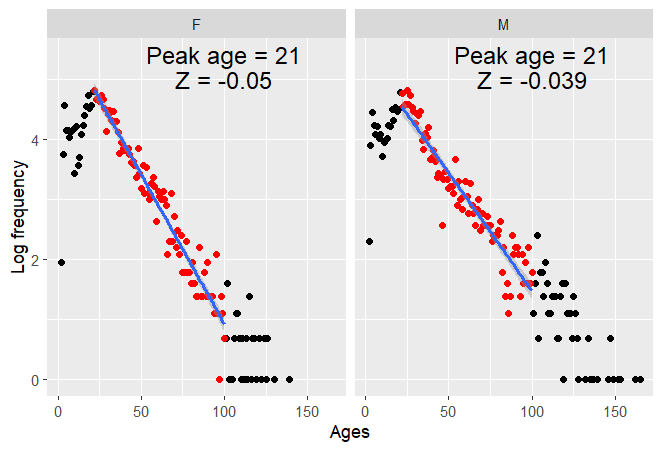
\includegraphics{plots_4_doc/Catch_curve_plot_FM_21_100.png}

}

\caption{\label{fig-CC_Z_100}Catch curve (log abundance by age) analysis
on aggregated ages over all age sources by sex (black points). The peak
selected age was 21 for both sexes with a max age of 100, so the linear
model was run from age 21 until age 100 (red points). The slope of the
linear model is equal to the estimate of an aggregate total mortality
(Z).}

\end{figure}%

\begin{figure}[H]

\centering{

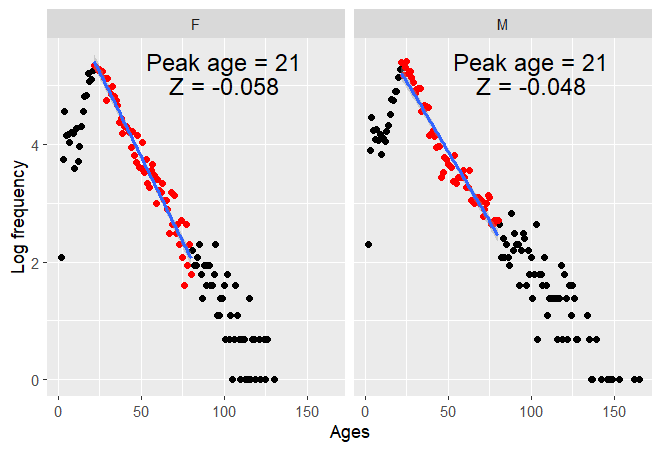
\includegraphics{plots_4_doc/Catch_curve_plot_FM_21_80.png}

}

\caption{\label{fig-CC_Z_80}Catch curve (log abundance by age) analysis
on aggregated ages over all age sources by sex (black points). The peak
selected age was 21 for both sexes with a max age of 80, so the linear
model was run from age 21 until age 80 (red points). The slope of the
linear model is equal to the estimate of an aggregate total mortality
(Z).}

\end{figure}%

\begin{figure}[H]

\centering{

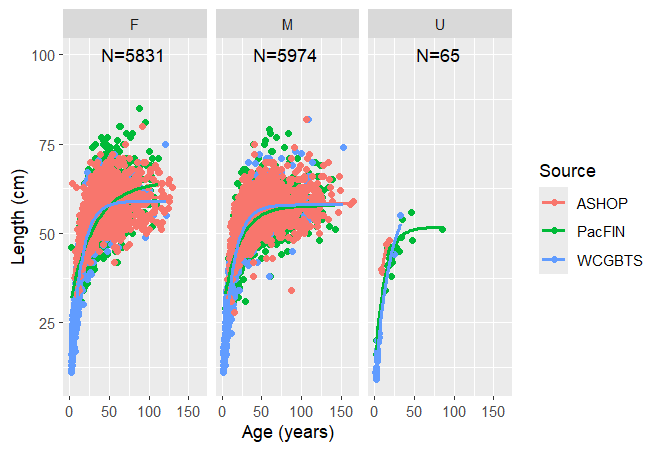
\includegraphics{plots_4_doc/Age_length_plot.png}

}

\caption{\label{fig-AL_1}Age and length data, with fitted von
Bertalanffy growth curves, by sex and data source for the
Rougheye/Blackspotted rockfish complex. Sample sizes (N) are also
provided.}

\end{figure}%

\begin{figure}[H]

\centering{

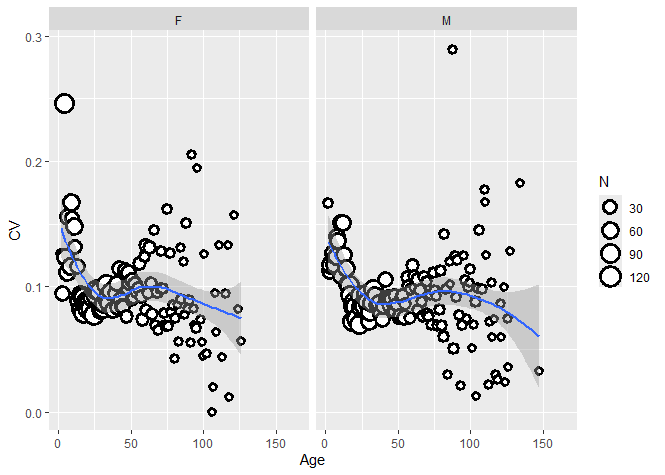
\includegraphics{plots_4_doc/Lt_age_CV_FM.png}

}

\caption{\label{fig-AL_2}Coefficient of variation by age and sex for all
sources of Rougheye/Blackspotted rockfishes ages. Sample sizes (N) are
also indicated by size of the point. The line is a smoothed loess
(polynomial) line that gives a moving average of CV by age and sex.}

\end{figure}%

\begin{figure}[H]

\centering{

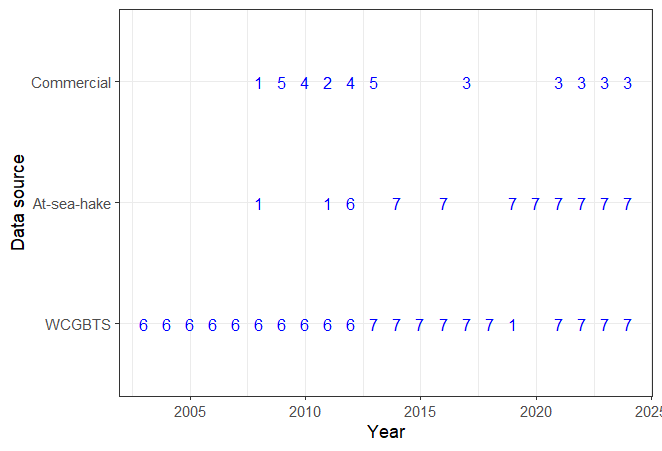
\includegraphics{plots_4_doc/AE_matrix_plot.png}

}

\caption{\label{fig-AE_matrices}Ageing error matrix assignments by year
and data source. The number indicates which ageing error matrix was used
for conditional ages within those years and data sources. `Commercial'
is a combination of all commercial fleets.}

\end{figure}%

\begin{figure}[H]

\centering{

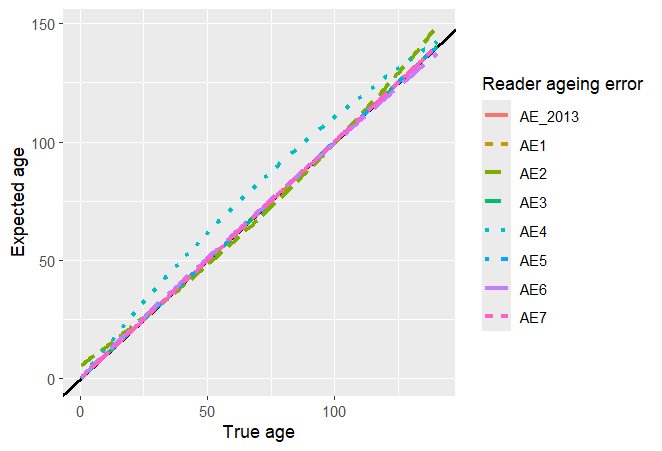
\includegraphics{plots_4_doc/AE_Bias.png}

}

\caption{\label{fig-AE_bias}Estimated bias used for each of the seven
ageing error matrices.}

\end{figure}%

\begin{figure}[H]

\centering{

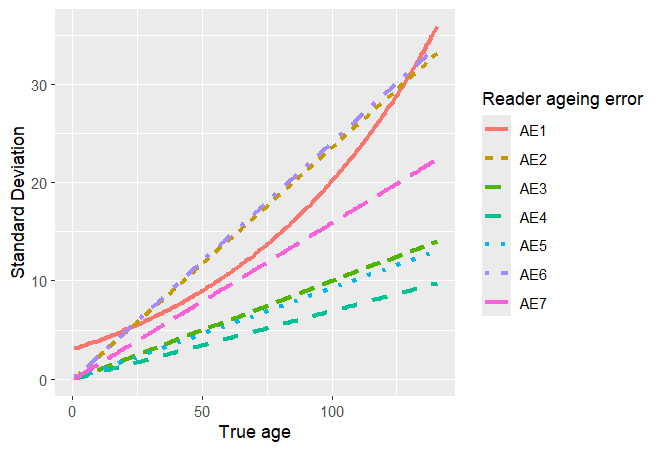
\includegraphics{plots_4_doc/AE_SD.png}

}

\caption{\label{fig-AE_SD}Estimated imprecision (as a standard
deviation) used for each of the seven ageing error matrices.}

\end{figure}%

\newpage

\begin{figure}[H]

\centering{

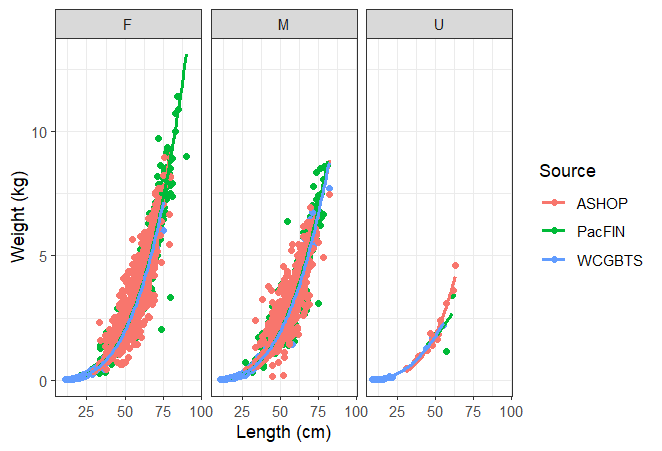
\includegraphics{plots_4_doc/L_W_plots.png}

}

\caption{\label{fig-LW1}Length and weight samples by sex and data
source. Lines are the power function fits by data source.}

\end{figure}%

\begin{figure}[H]

\centering{

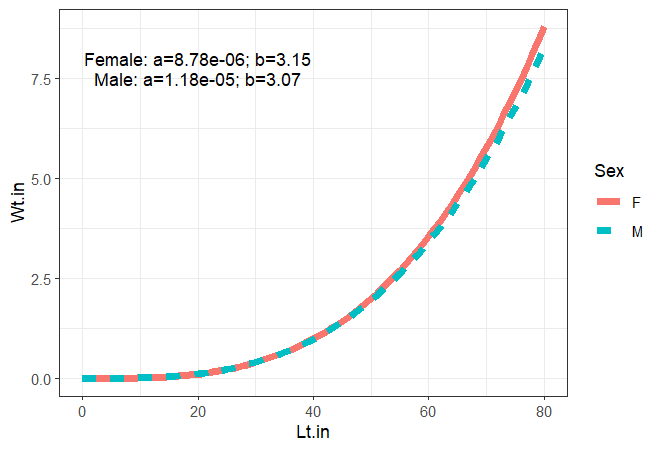
\includegraphics{plots_4_doc/F_M_ltwt_plot.png}

}

\caption{\label{fig-LW2}Realized length and weight relationships for
female and male Rougheye/Blackspotted Rockfishes.}

\end{figure}%

\newpage

\subsection{Model Bridging}\label{model-bridging}

\begin{figure}[H]

\centering{

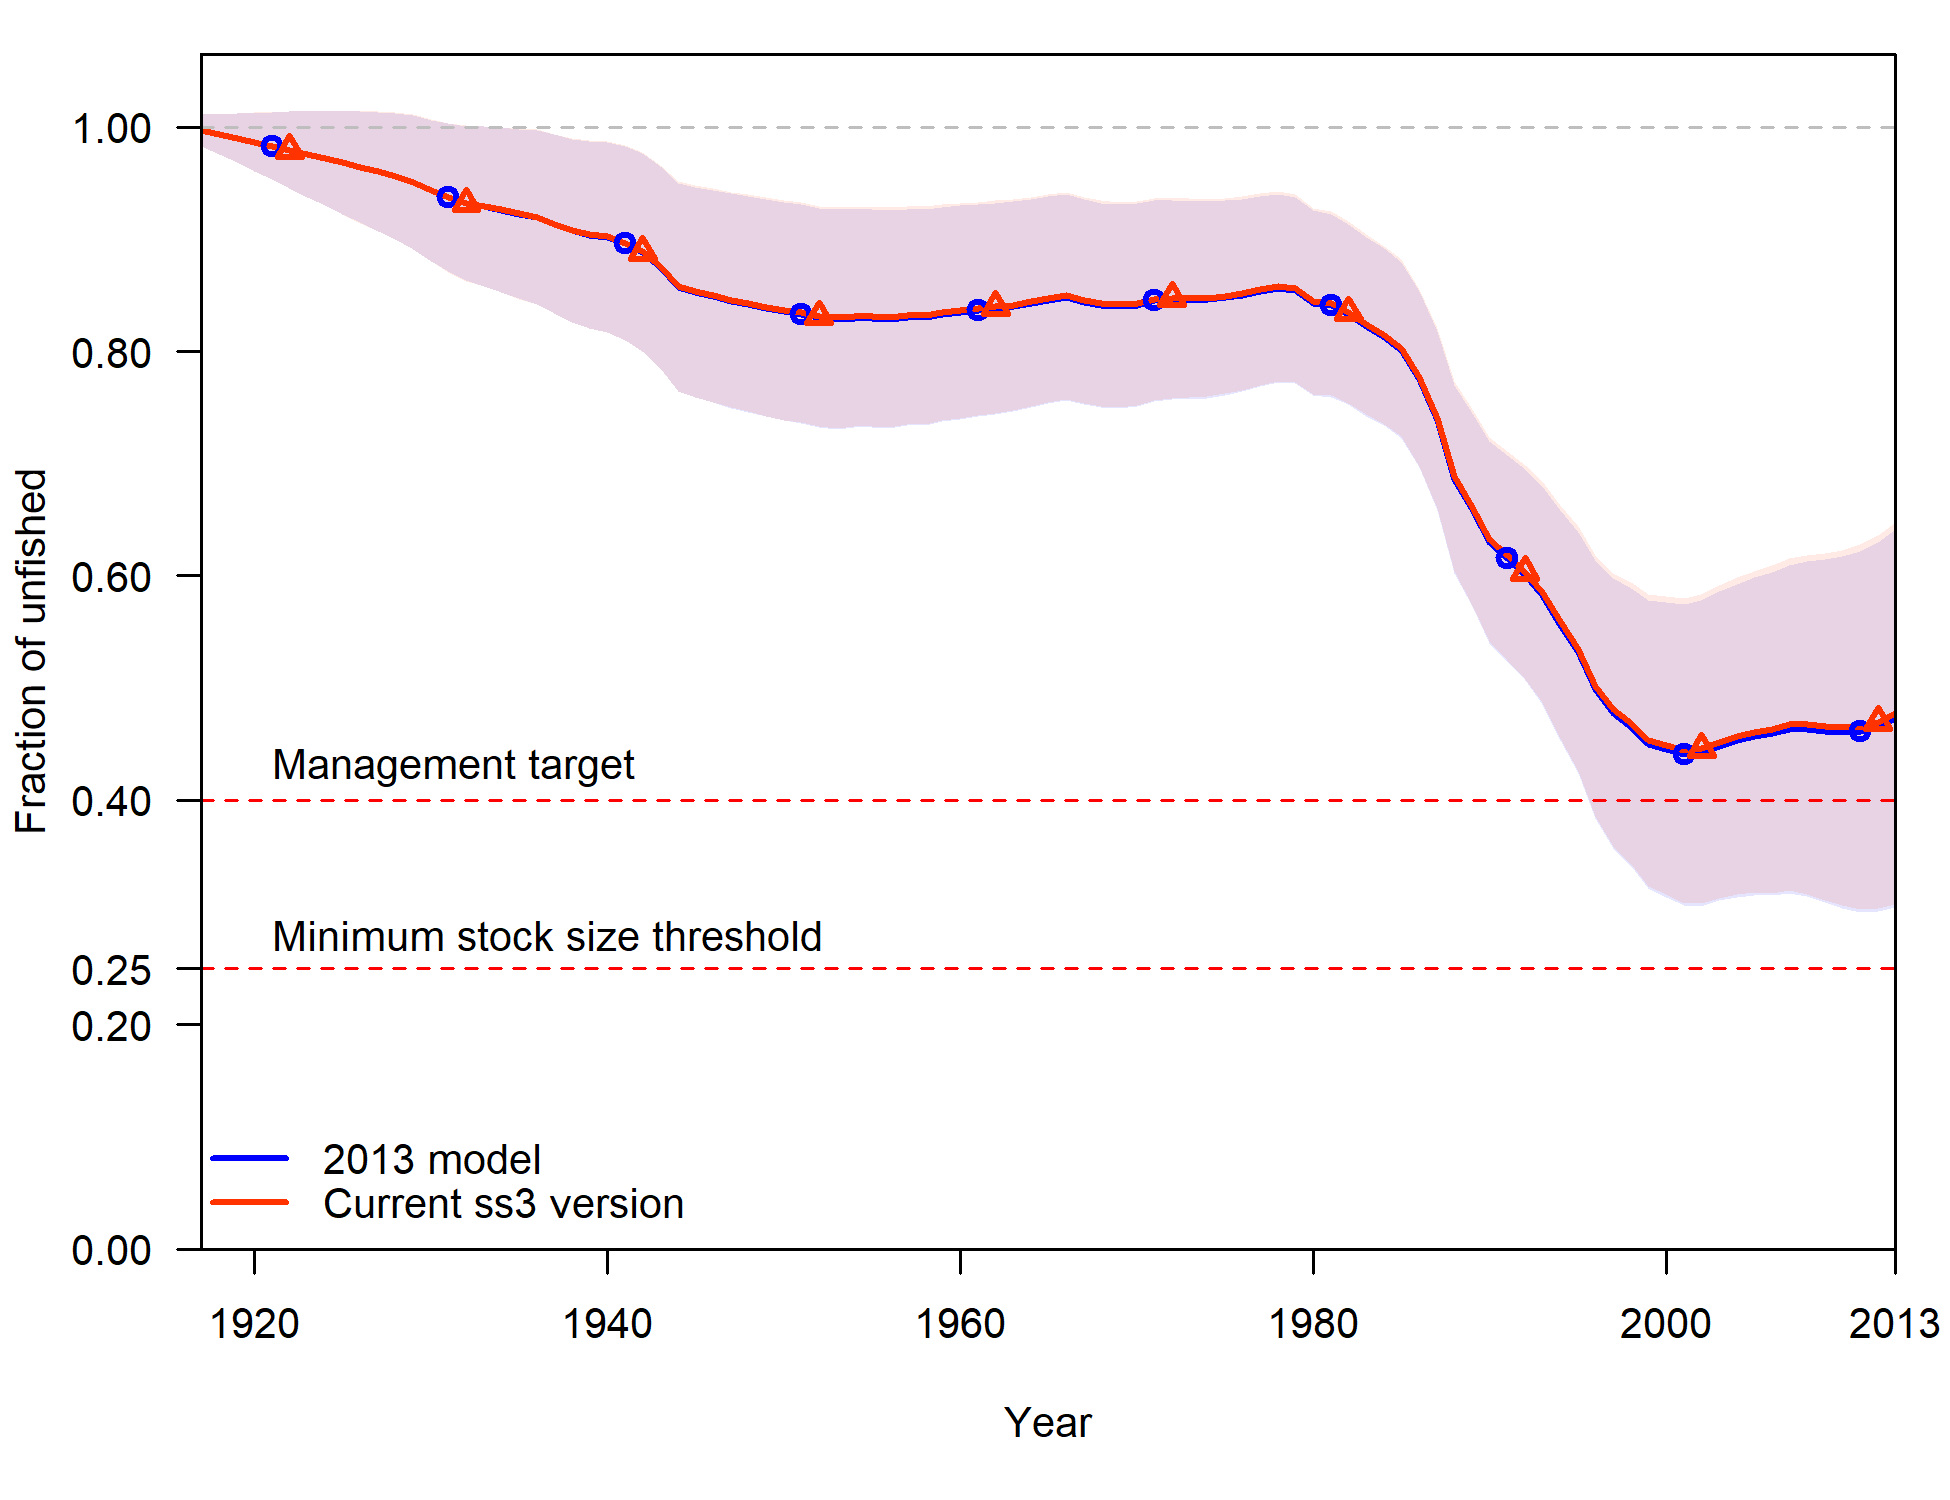
\includegraphics{plots_4_doc/compare4_Bratio_uncertainty.png}

}

\caption{\label{fig-RSS_2013}Estimates of relative stock size (current
spawning output/unfished spawning output) for the Rougheye/Blackspotted
rockfish complex in U.S. west coast waters from the 2013 assessment, and
compared to the using the same data in the newest version of SS3
(3.30.22.1).}

\end{figure}%

\begin{figure}[H]

\centering{

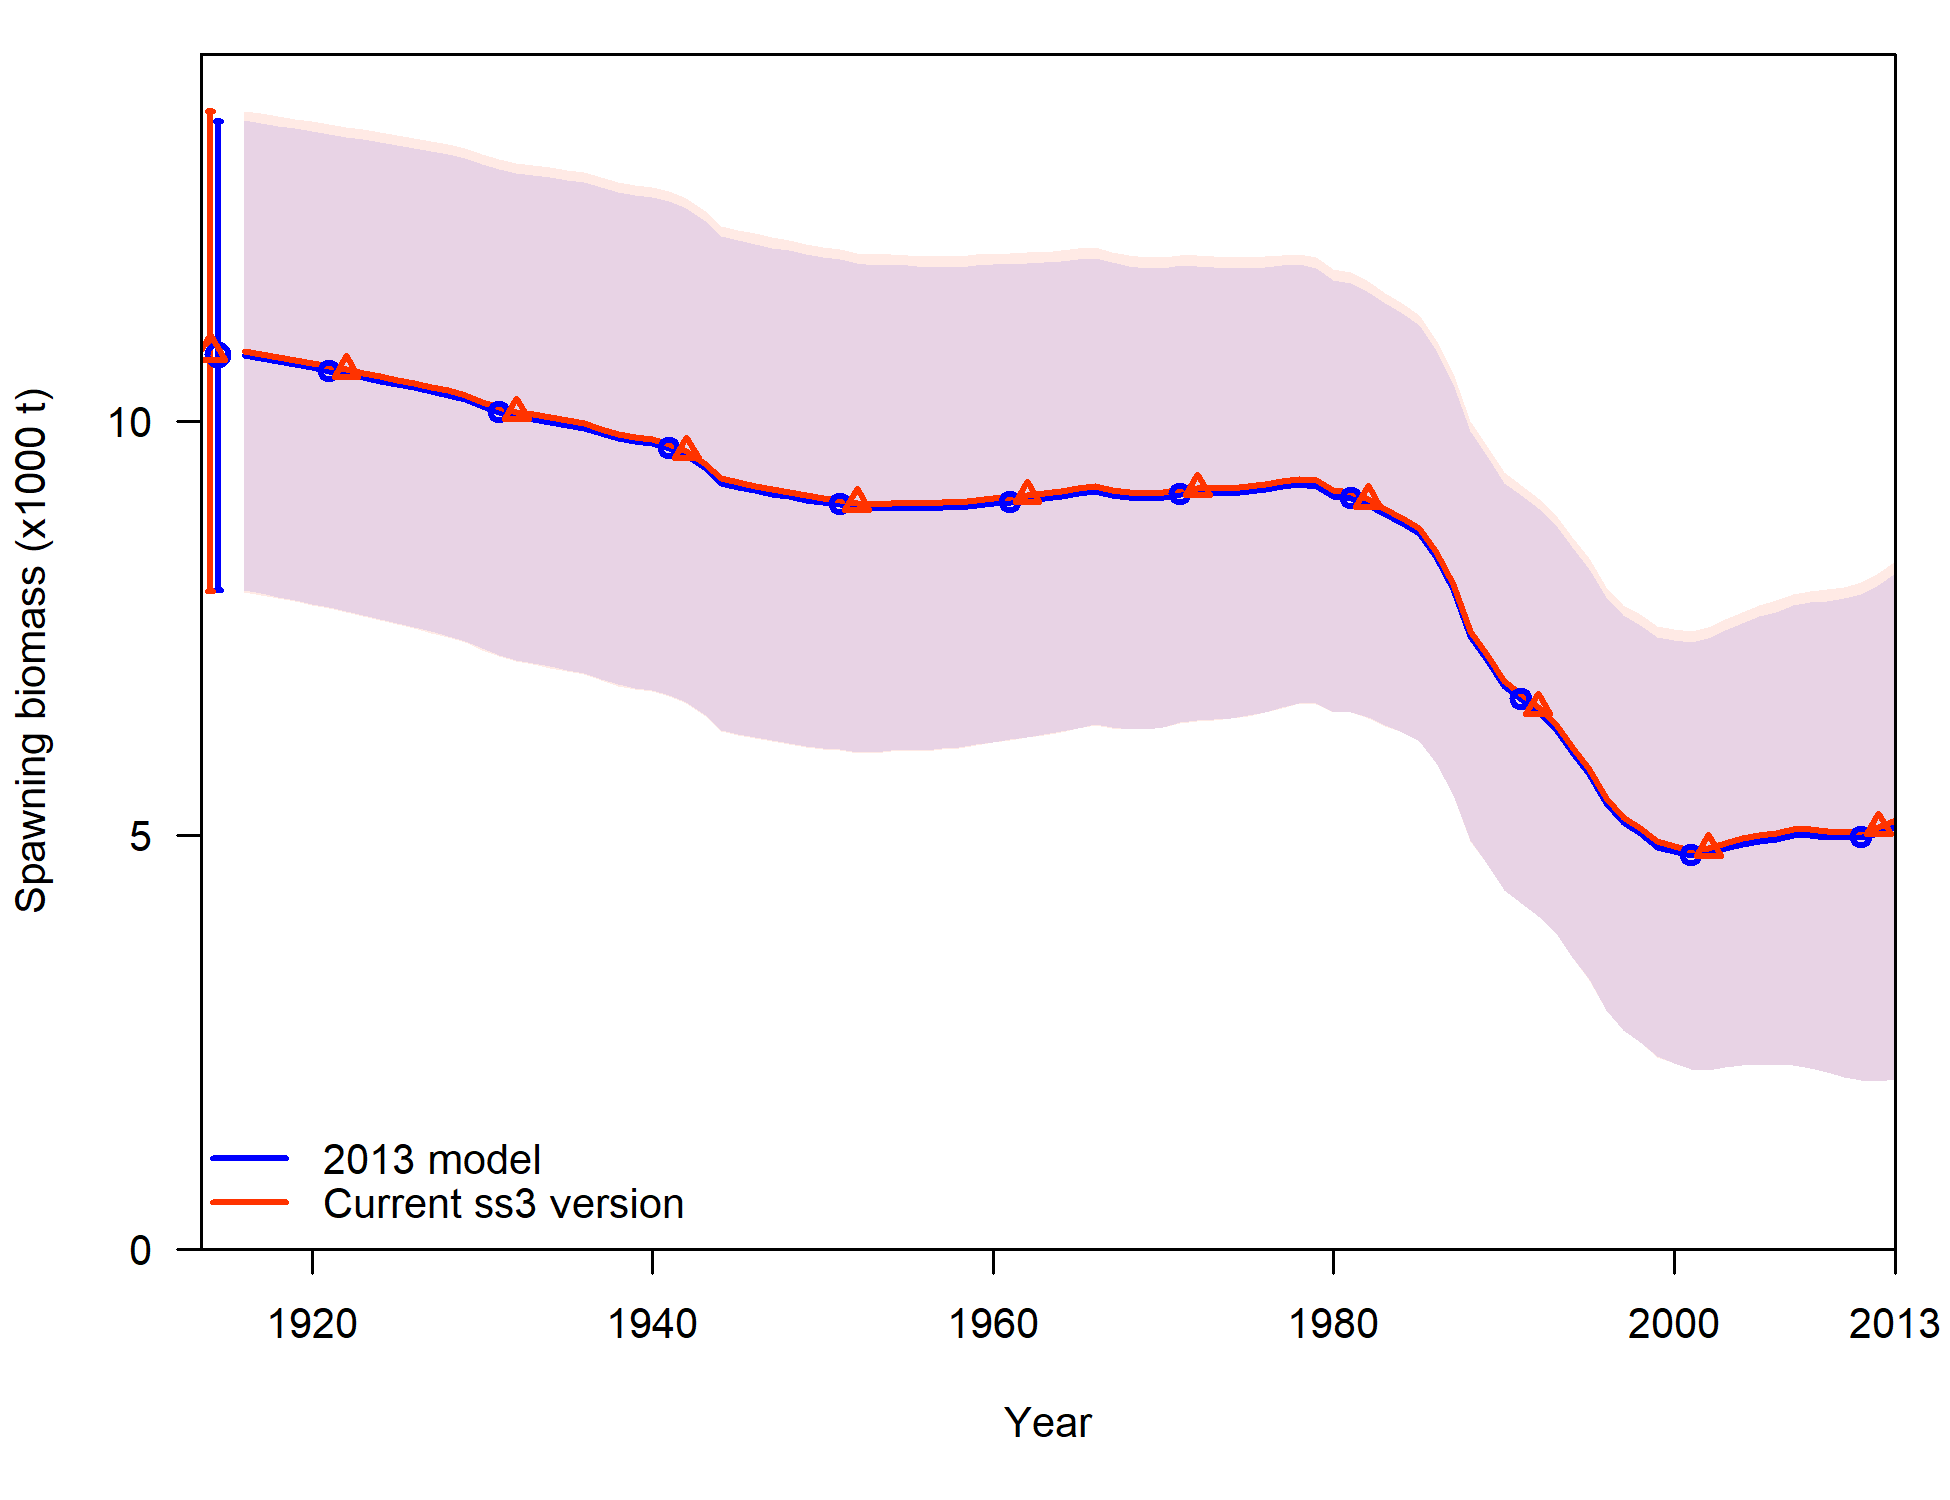
\includegraphics{plots_4_doc/compare2_spawnbio_uncertainty.png}

}

\caption{\label{fig-SO_2013}Estimates of spawning output for the
Rougheye/Blackspotted rockfish complex in U.S. west coast waters from
the 2013 assessment, and compared to the same data in the newest version
of SS3 (3.30.22.1). Shading denotes 95\% confidence intervals. Shading
denotes 95\% confidence intervals.}

\end{figure}%

\newpage

\subsection{Model Specification}\label{model-specification}

\begin{figure}[H]

\centering{

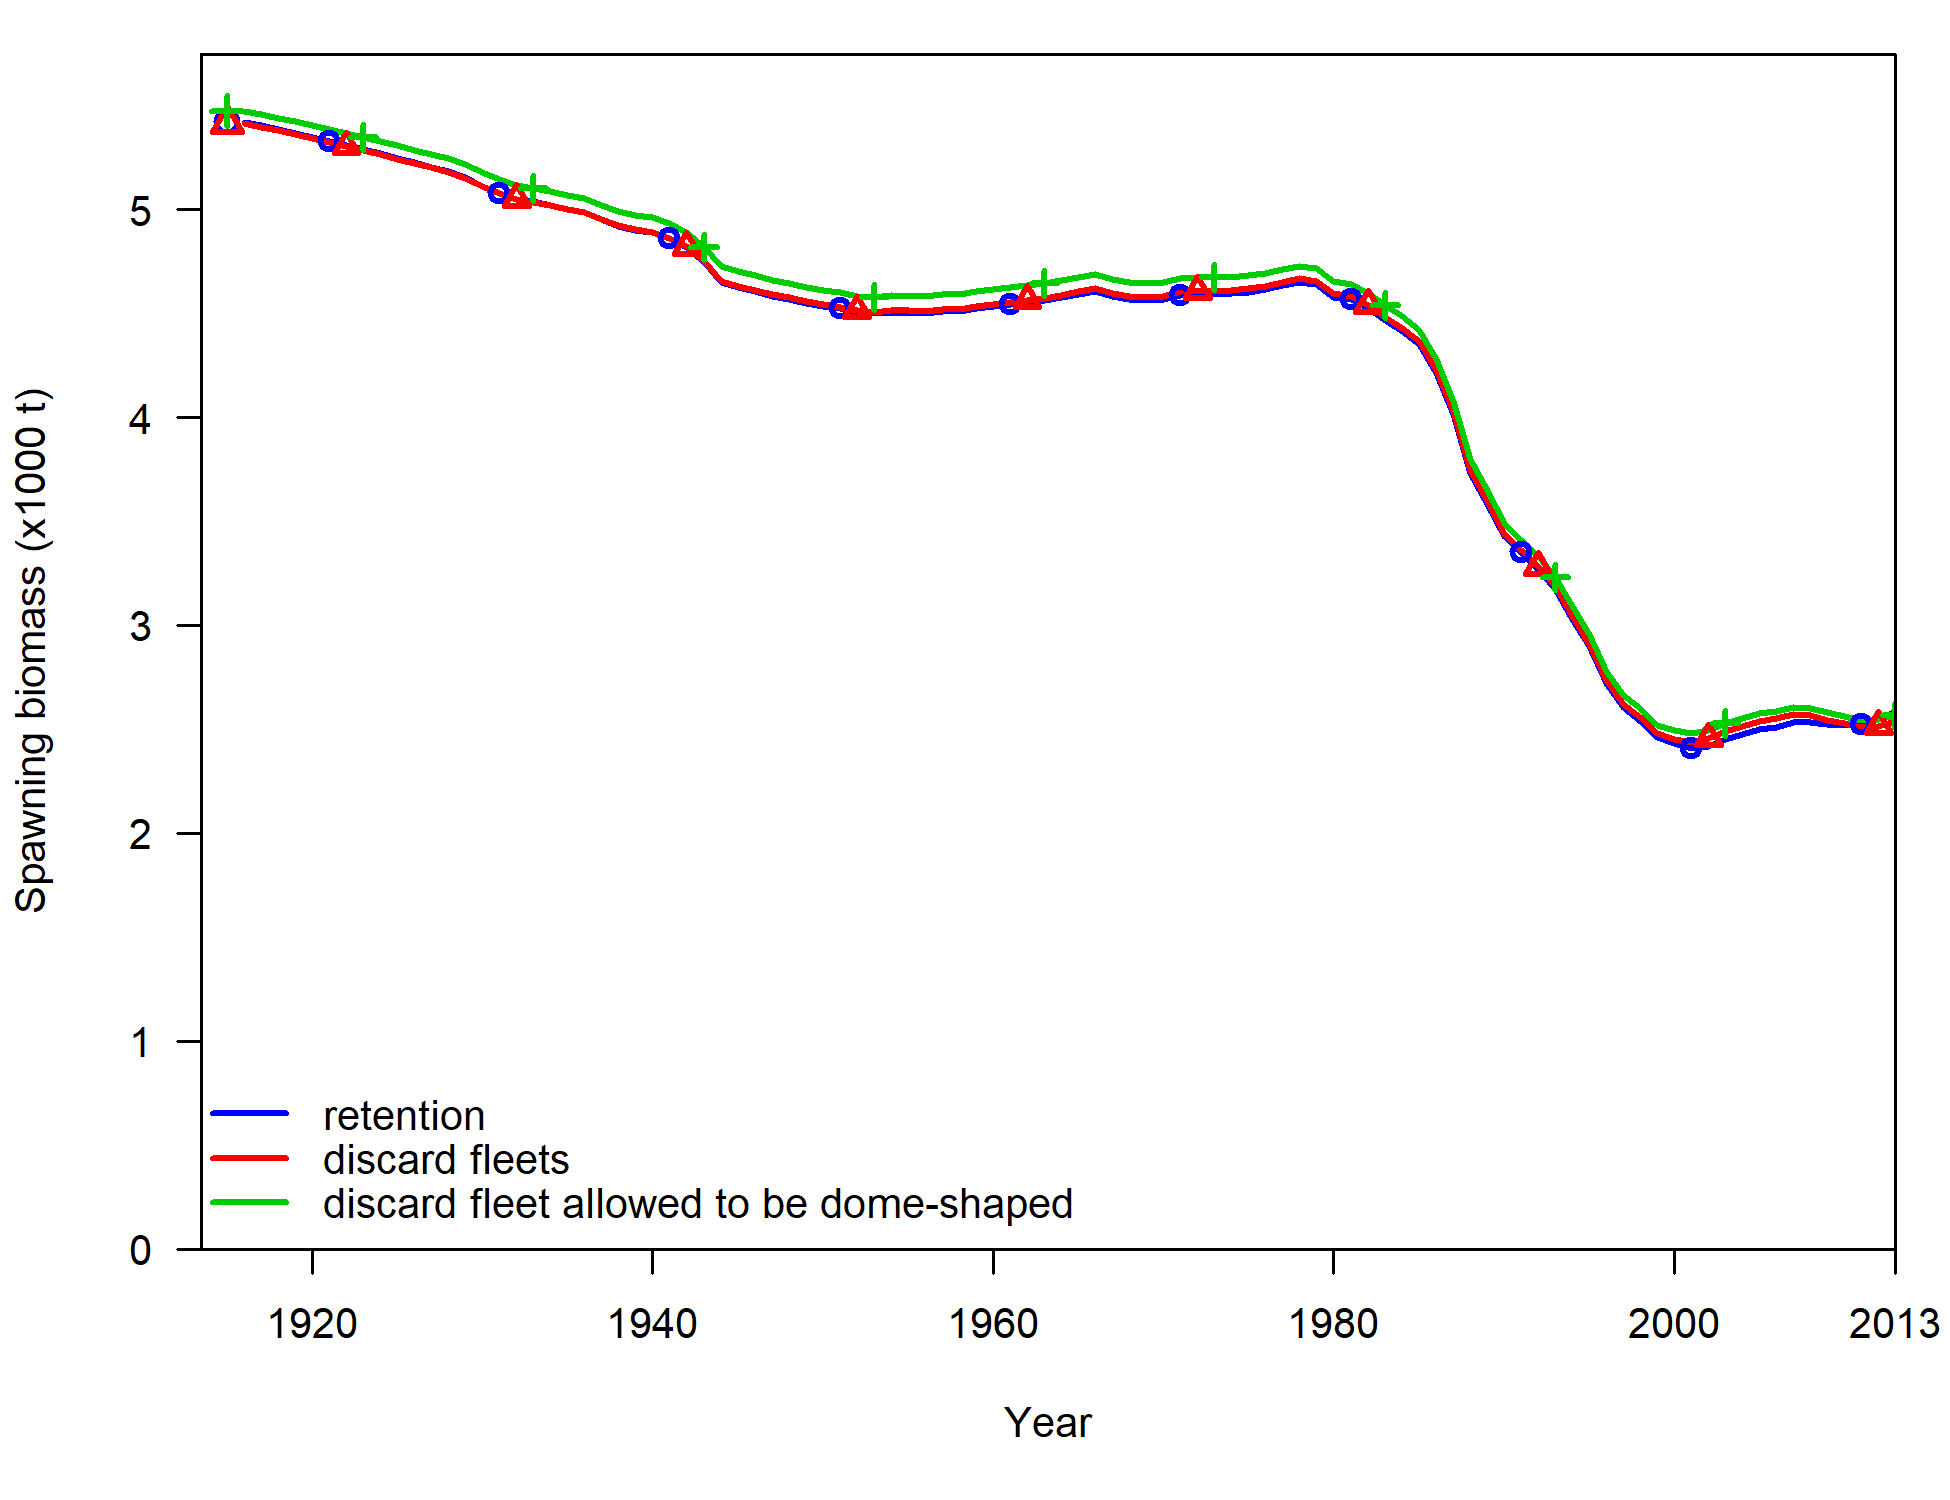
\includegraphics{plots_4_doc/compare1_spawnbio__discard_fleets.png}

}

\caption{\label{fig-Discard_comp_SO}Comparison of spawning output using
retention curves or discard fleets using the 2013 Rougheye/Blackspotted
Rockfishes assessment.}

\end{figure}%

\begin{figure}[H]

\centering{

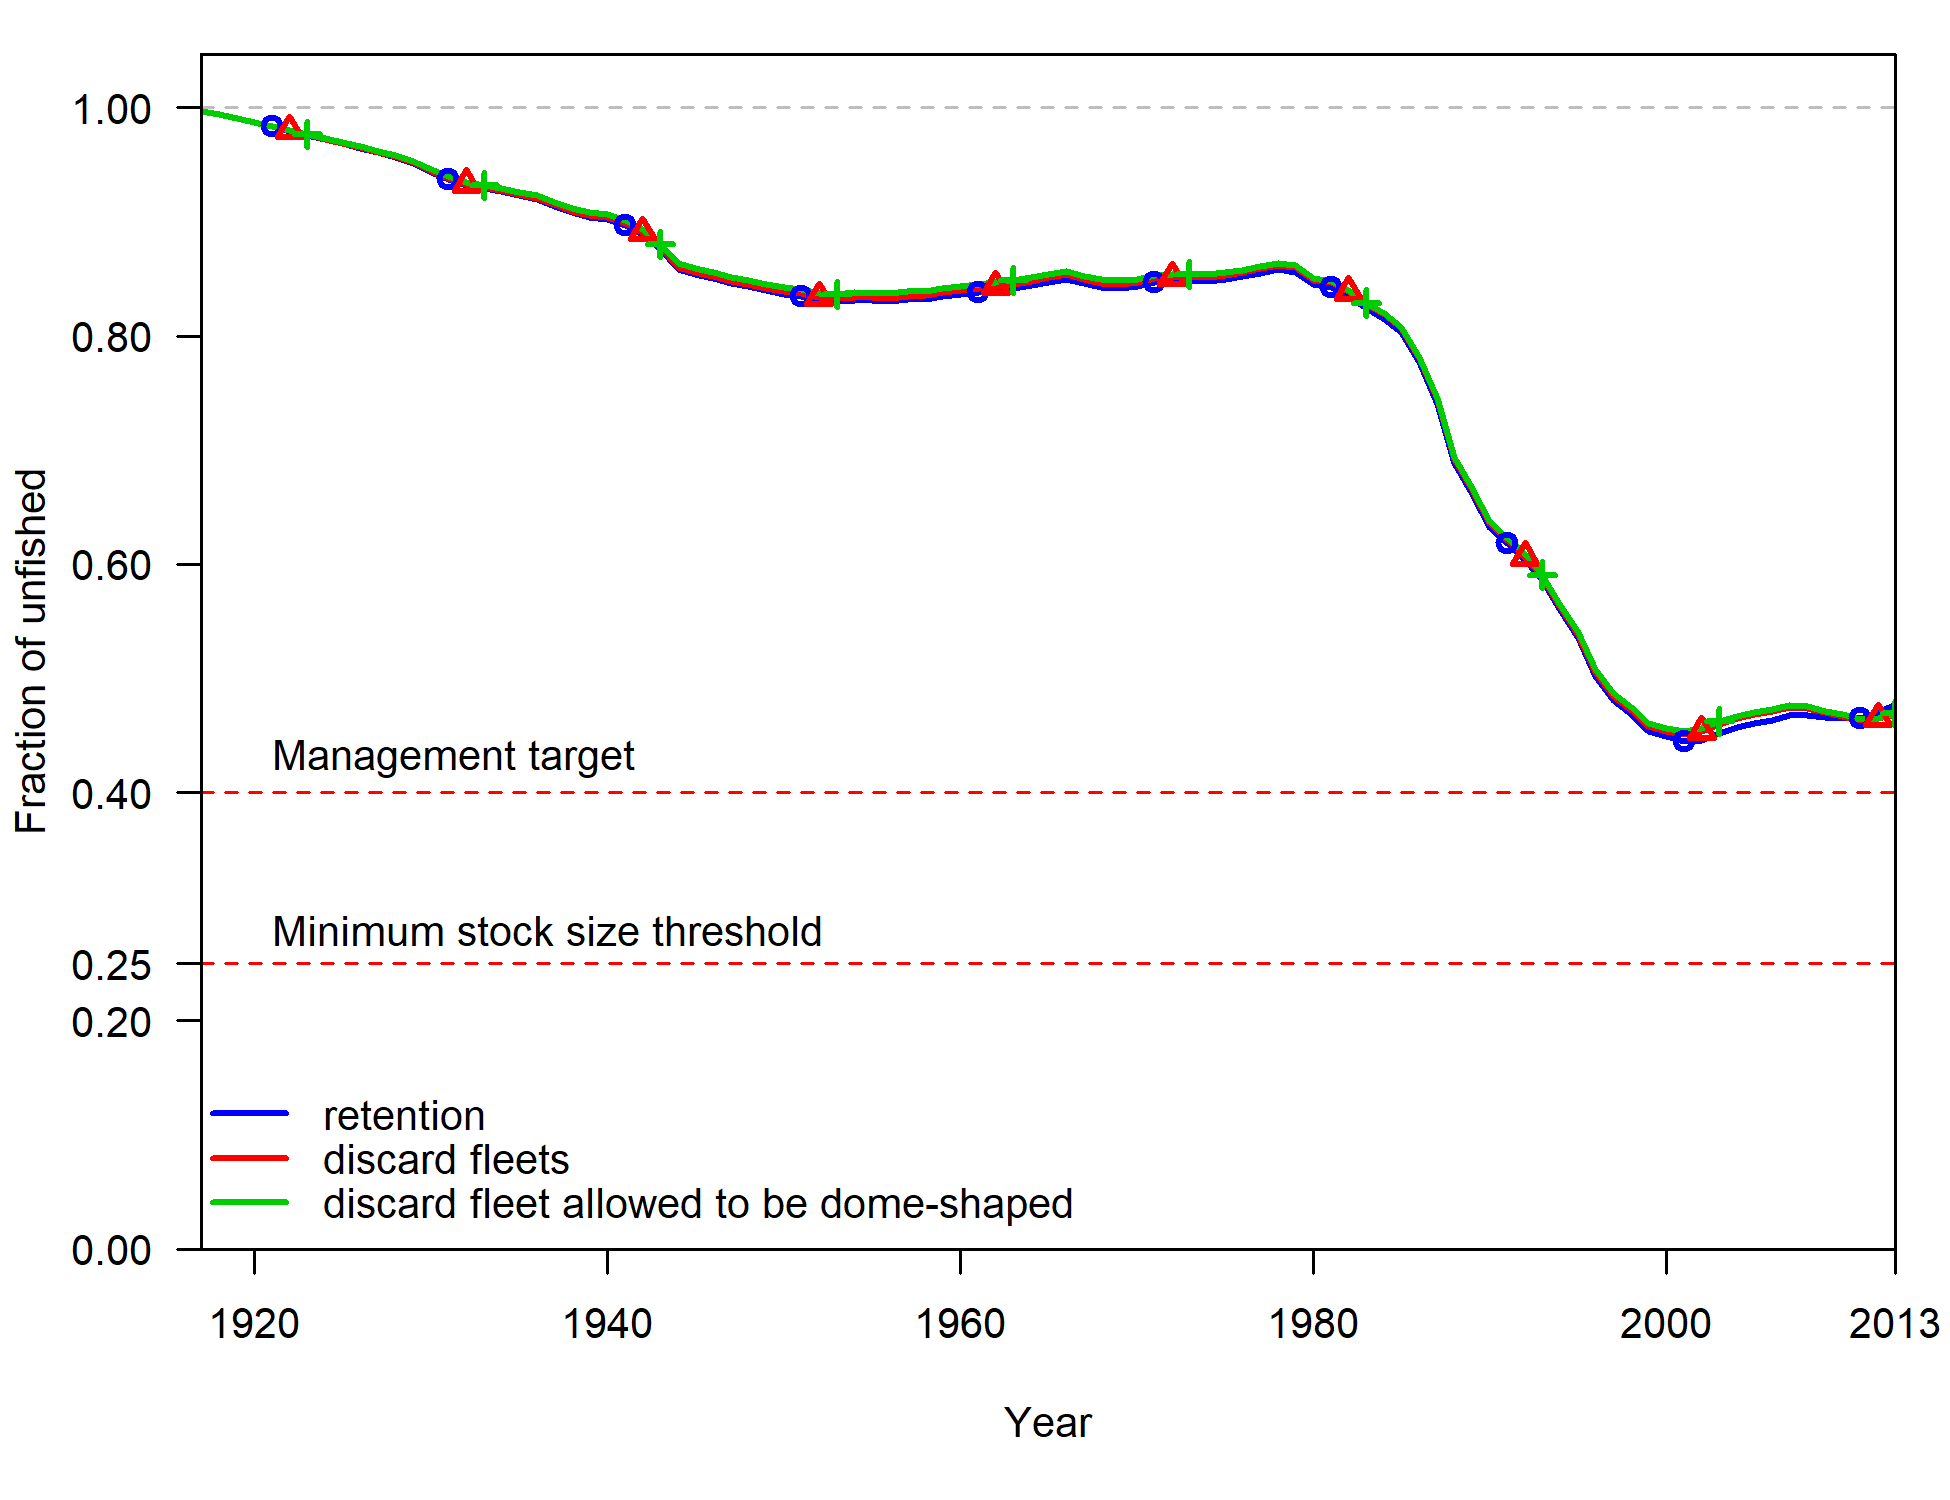
\includegraphics{plots_4_doc/compare3_Bratio_discard_fleets.png}

}

\caption{\label{fig-Discard_comp_RSS}Comparison of relative spawning
output using retention curves or discard fleets using the 2013
Rougheye/Blackspotted Rockfishes assessment.}

\end{figure}%

\begin{figure}[H]

\centering{

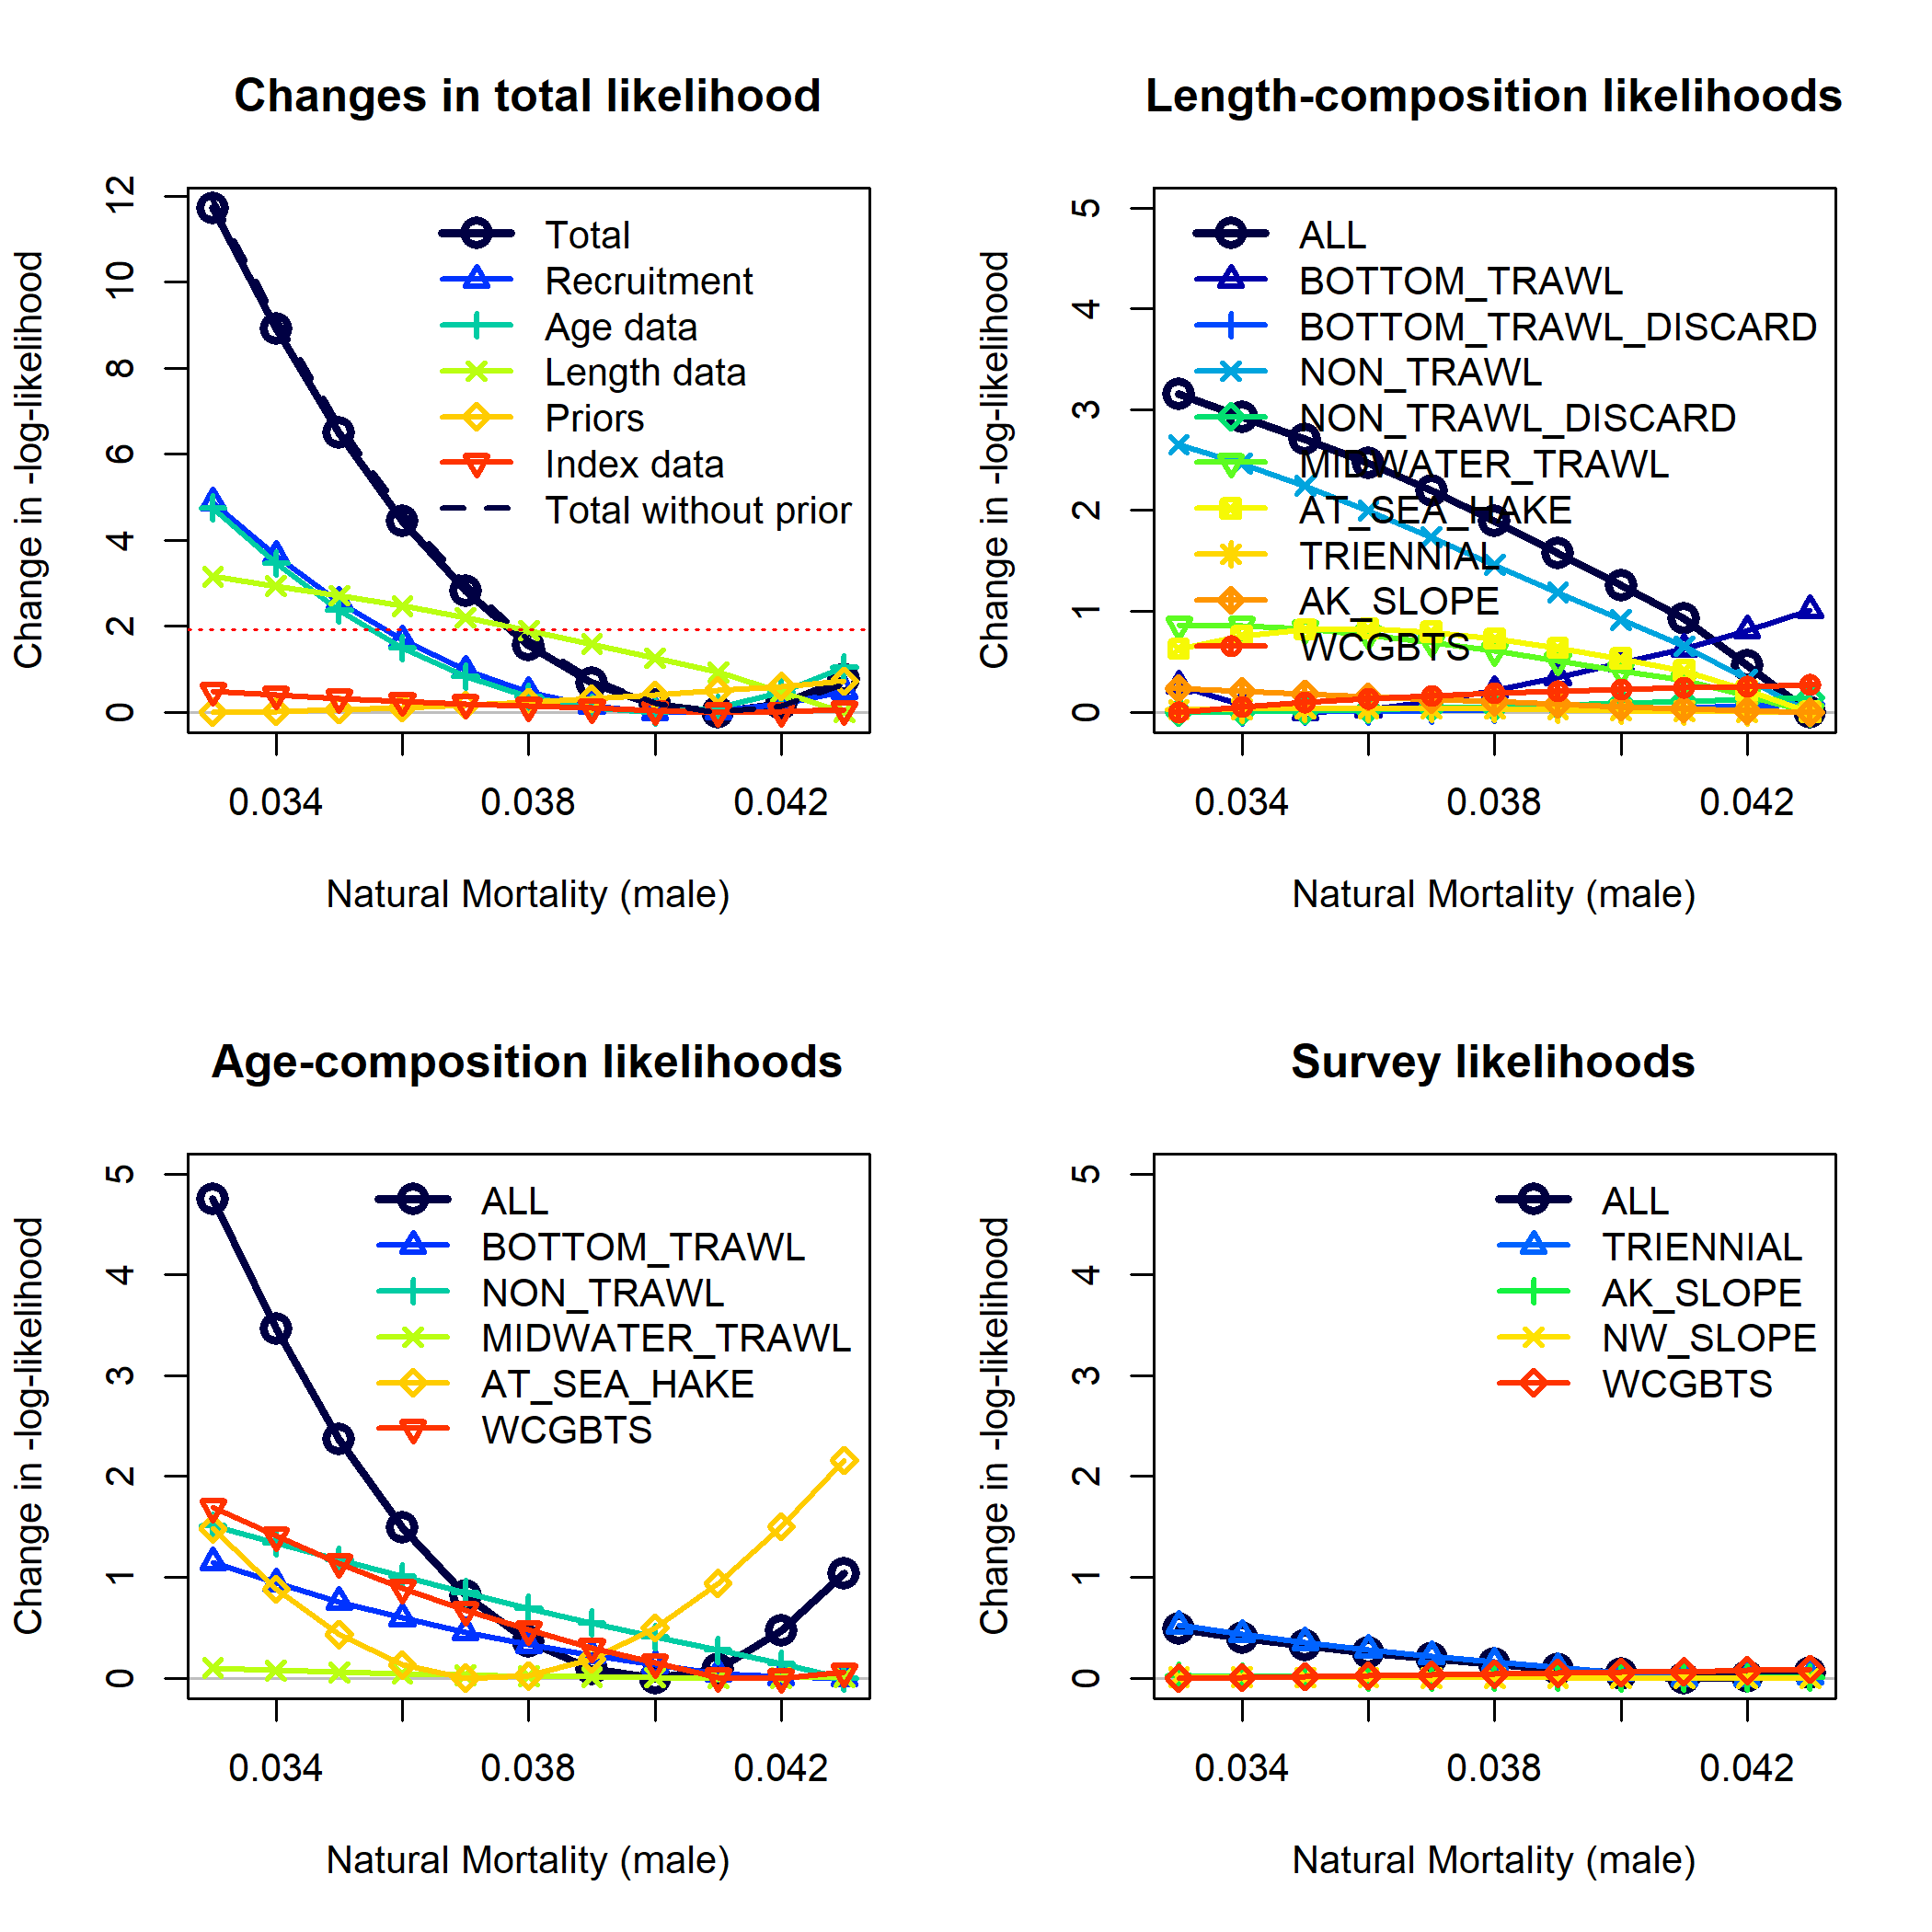
\includegraphics{plots_4_doc/piner_panel_NatM_uniform_Mal_GP_1.png}

}

\caption{\label{fig-M-profile-explore}Likelihood profile and component
likelihoods used to establish a fixed value for male natural mortality.}

\end{figure}%

\newpage

\subsection{Model convergence and fits to
data}\label{model-convergence-and-fits-to-data}

\begin{figure}[H]

\centering{

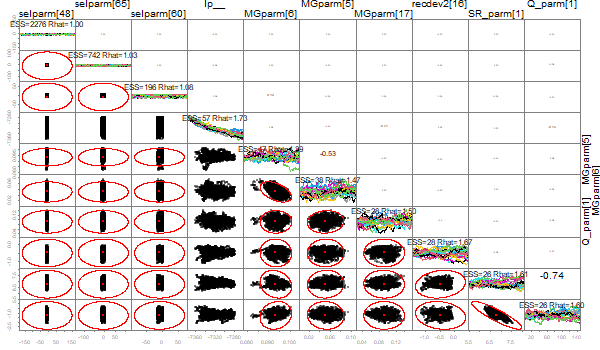
\includegraphics{plots_4_doc/pairs_plot_fast.png}

}

\caption{\label{fig-pairs_plot_fast}Pairs plots of the fastest mixing
parameters from running 2000 posterior draws (keeping every draw) using
the random walk Metropolis algorithm. Parameters that show little to no
movement are recommended to be fixed to improve model speed and
efficiency.}

\end{figure}%

\begin{figure}[H]

\centering{

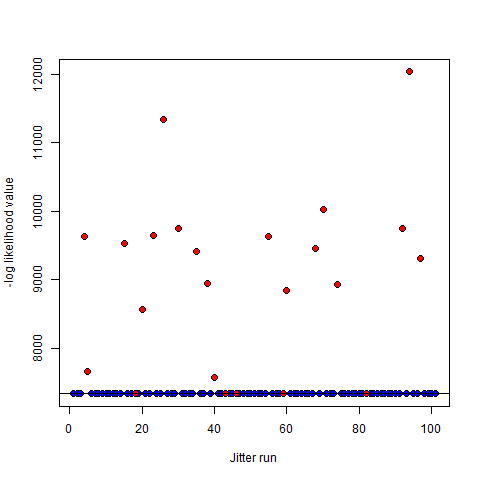
\includegraphics{ref_model/Jitter Results_0.01/jitterplot.png}

}

\caption{\label{fig-jitter001}Jitter runs (using a value of 0.01) for
the reference model, with jitter run number on the x-axis and -log
likelihood value on the y-axis. Blue dot are models that match the
likelihood value of the reference model, while red dots deviate from the
reference model. All red dots are above the blue dots, indicating no
better fit to the reference model was found.}

\end{figure}%

\begin{figure}[H]

\centering{

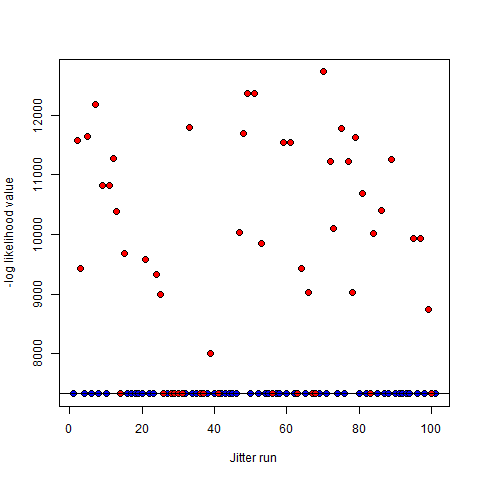
\includegraphics{ref_model/Jitter Results_0.05/jitterplot.png}

}

\caption{\label{fig-jitter005}Jitter runs (using a value of 0.05) for
the reference model, with jitter run number on the x-axis and -log
likelihood value on the y-axis. Blue dot are models that match the
likelihood value of the reference model, while red dots deviate from the
reference model. All red dots are above the blue dots, indicating no
better fit to the reference model was found.}

\end{figure}%

\subsection{Fits to data}\label{fits-to-data}

\begin{figure}[H]

\centering{

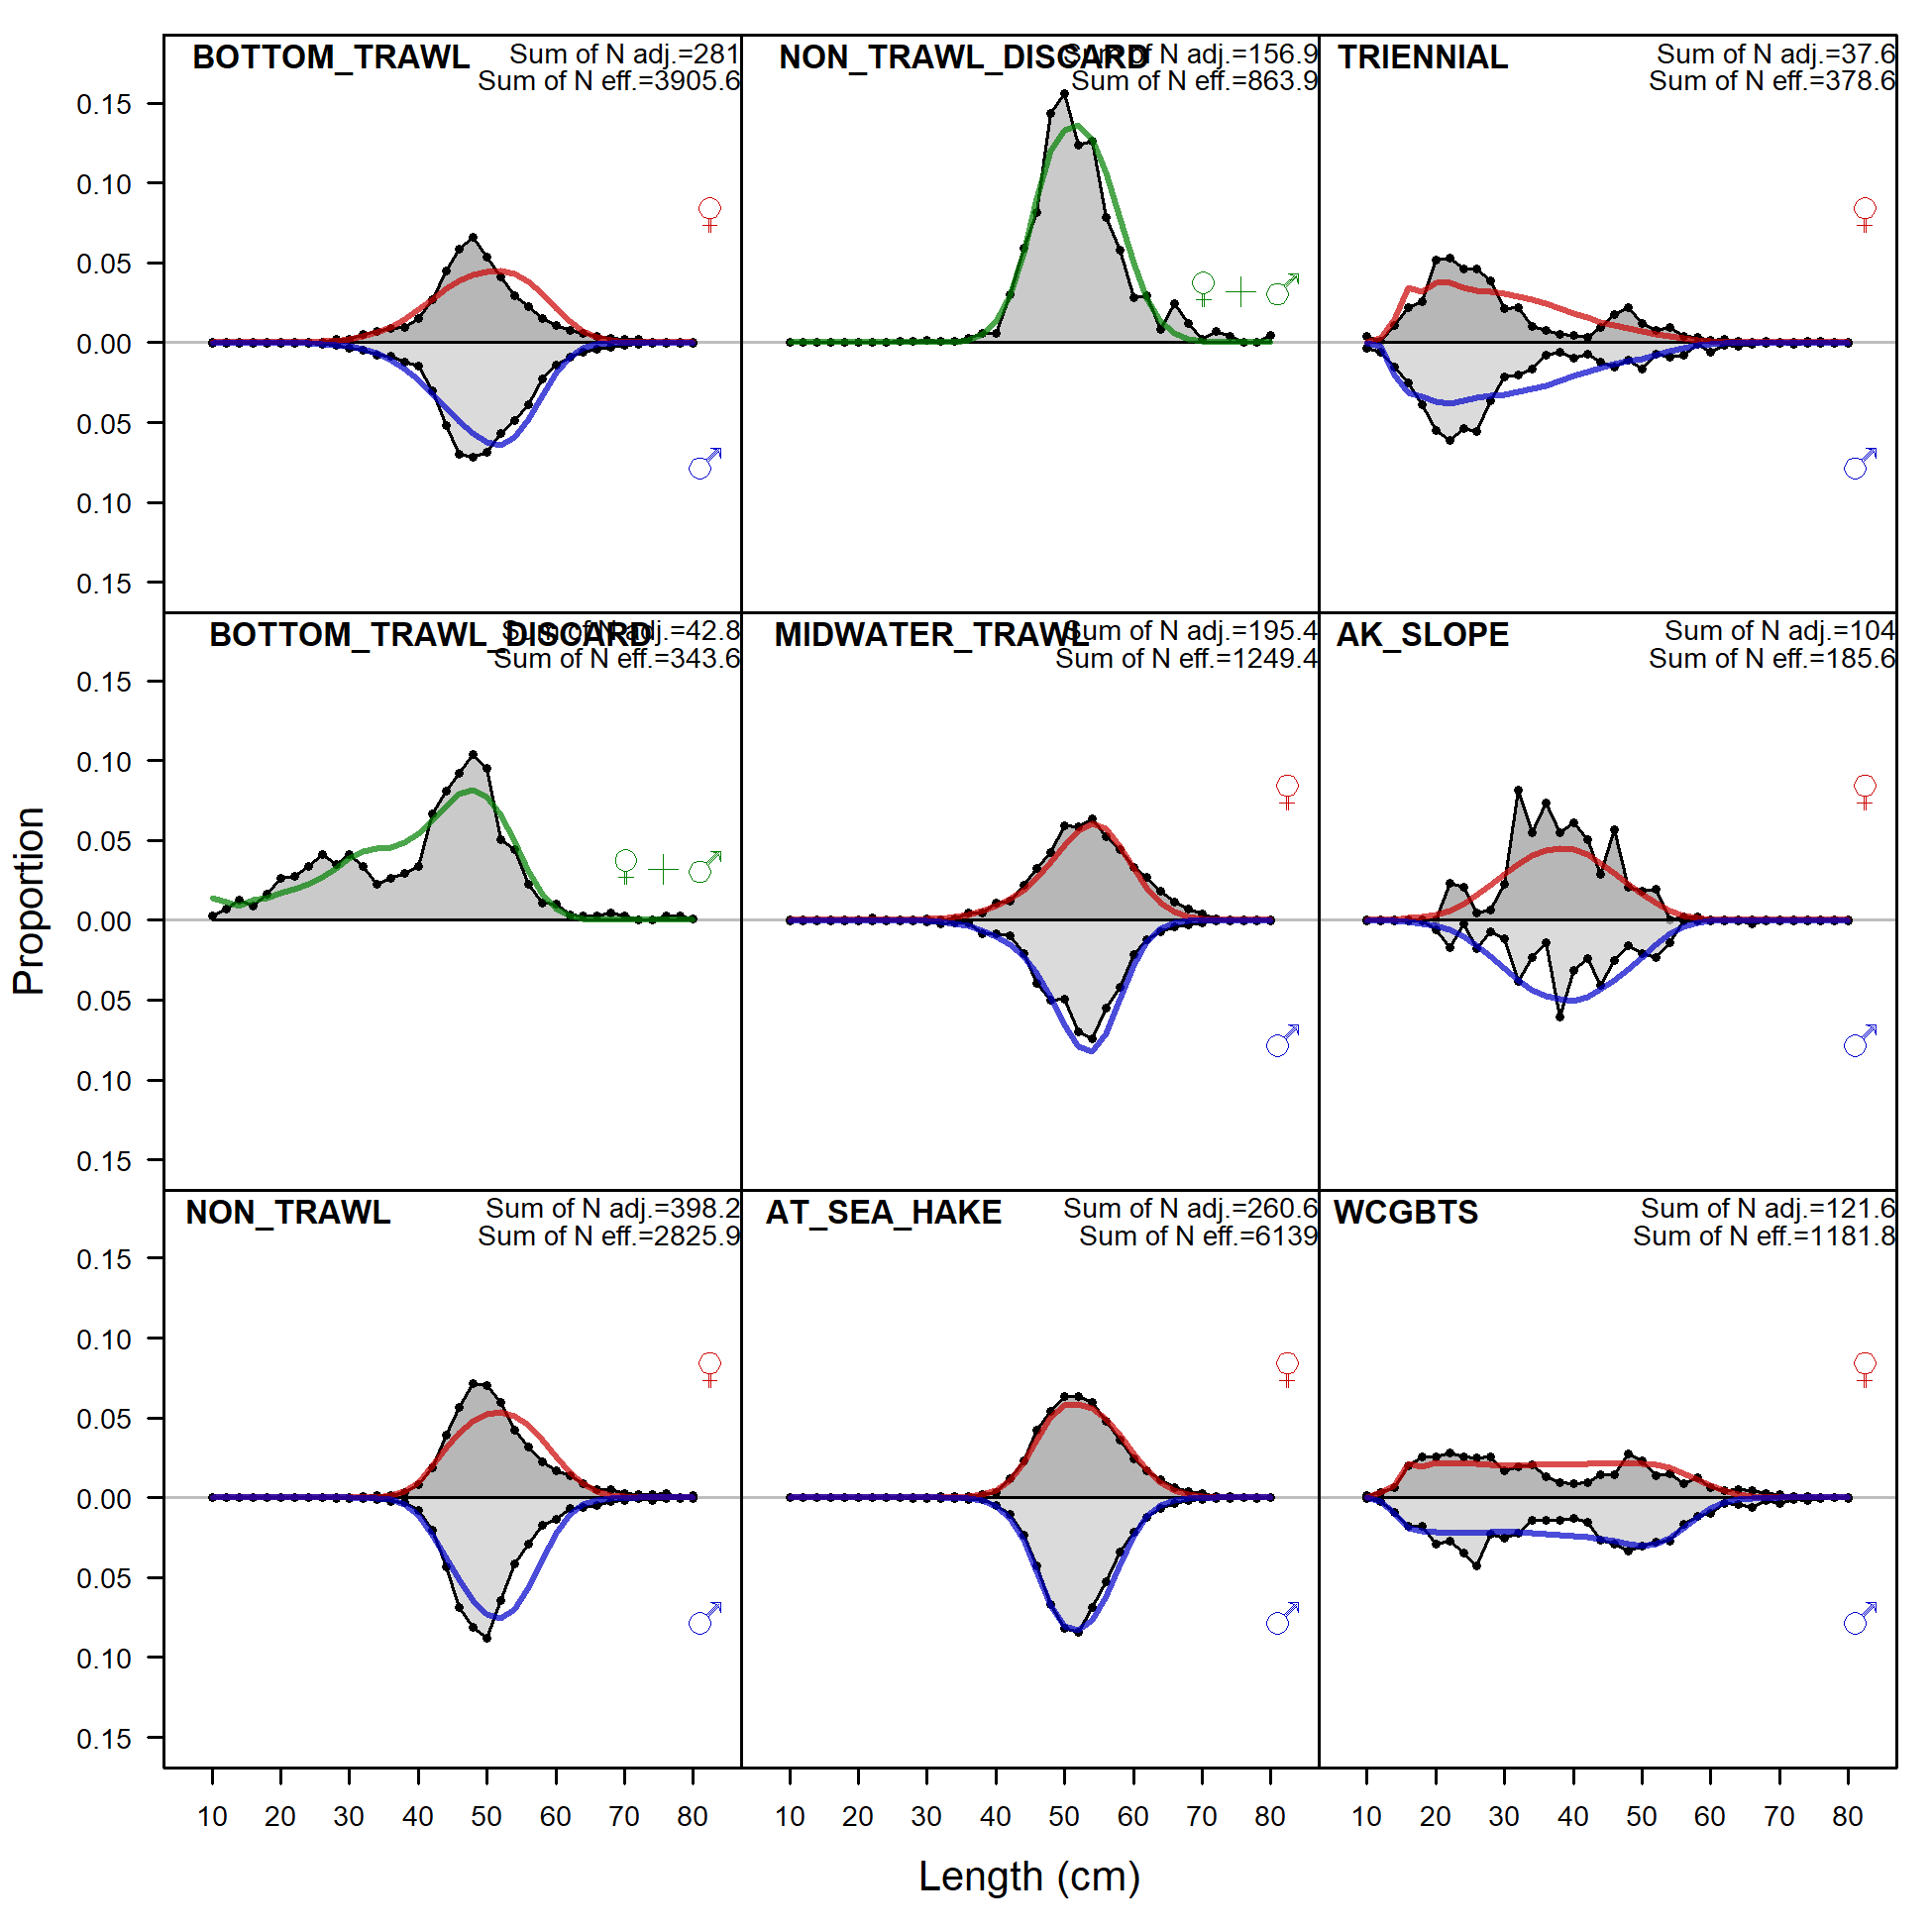
\includegraphics{ref_model/plots/comp_lenfit__aggregated_across_time.png}

}

\caption{\label{fig-agg-len-fit}Aggregated length (cm) compositions over
all years.}

\end{figure}%

\begin{figure}[H]

\centering{

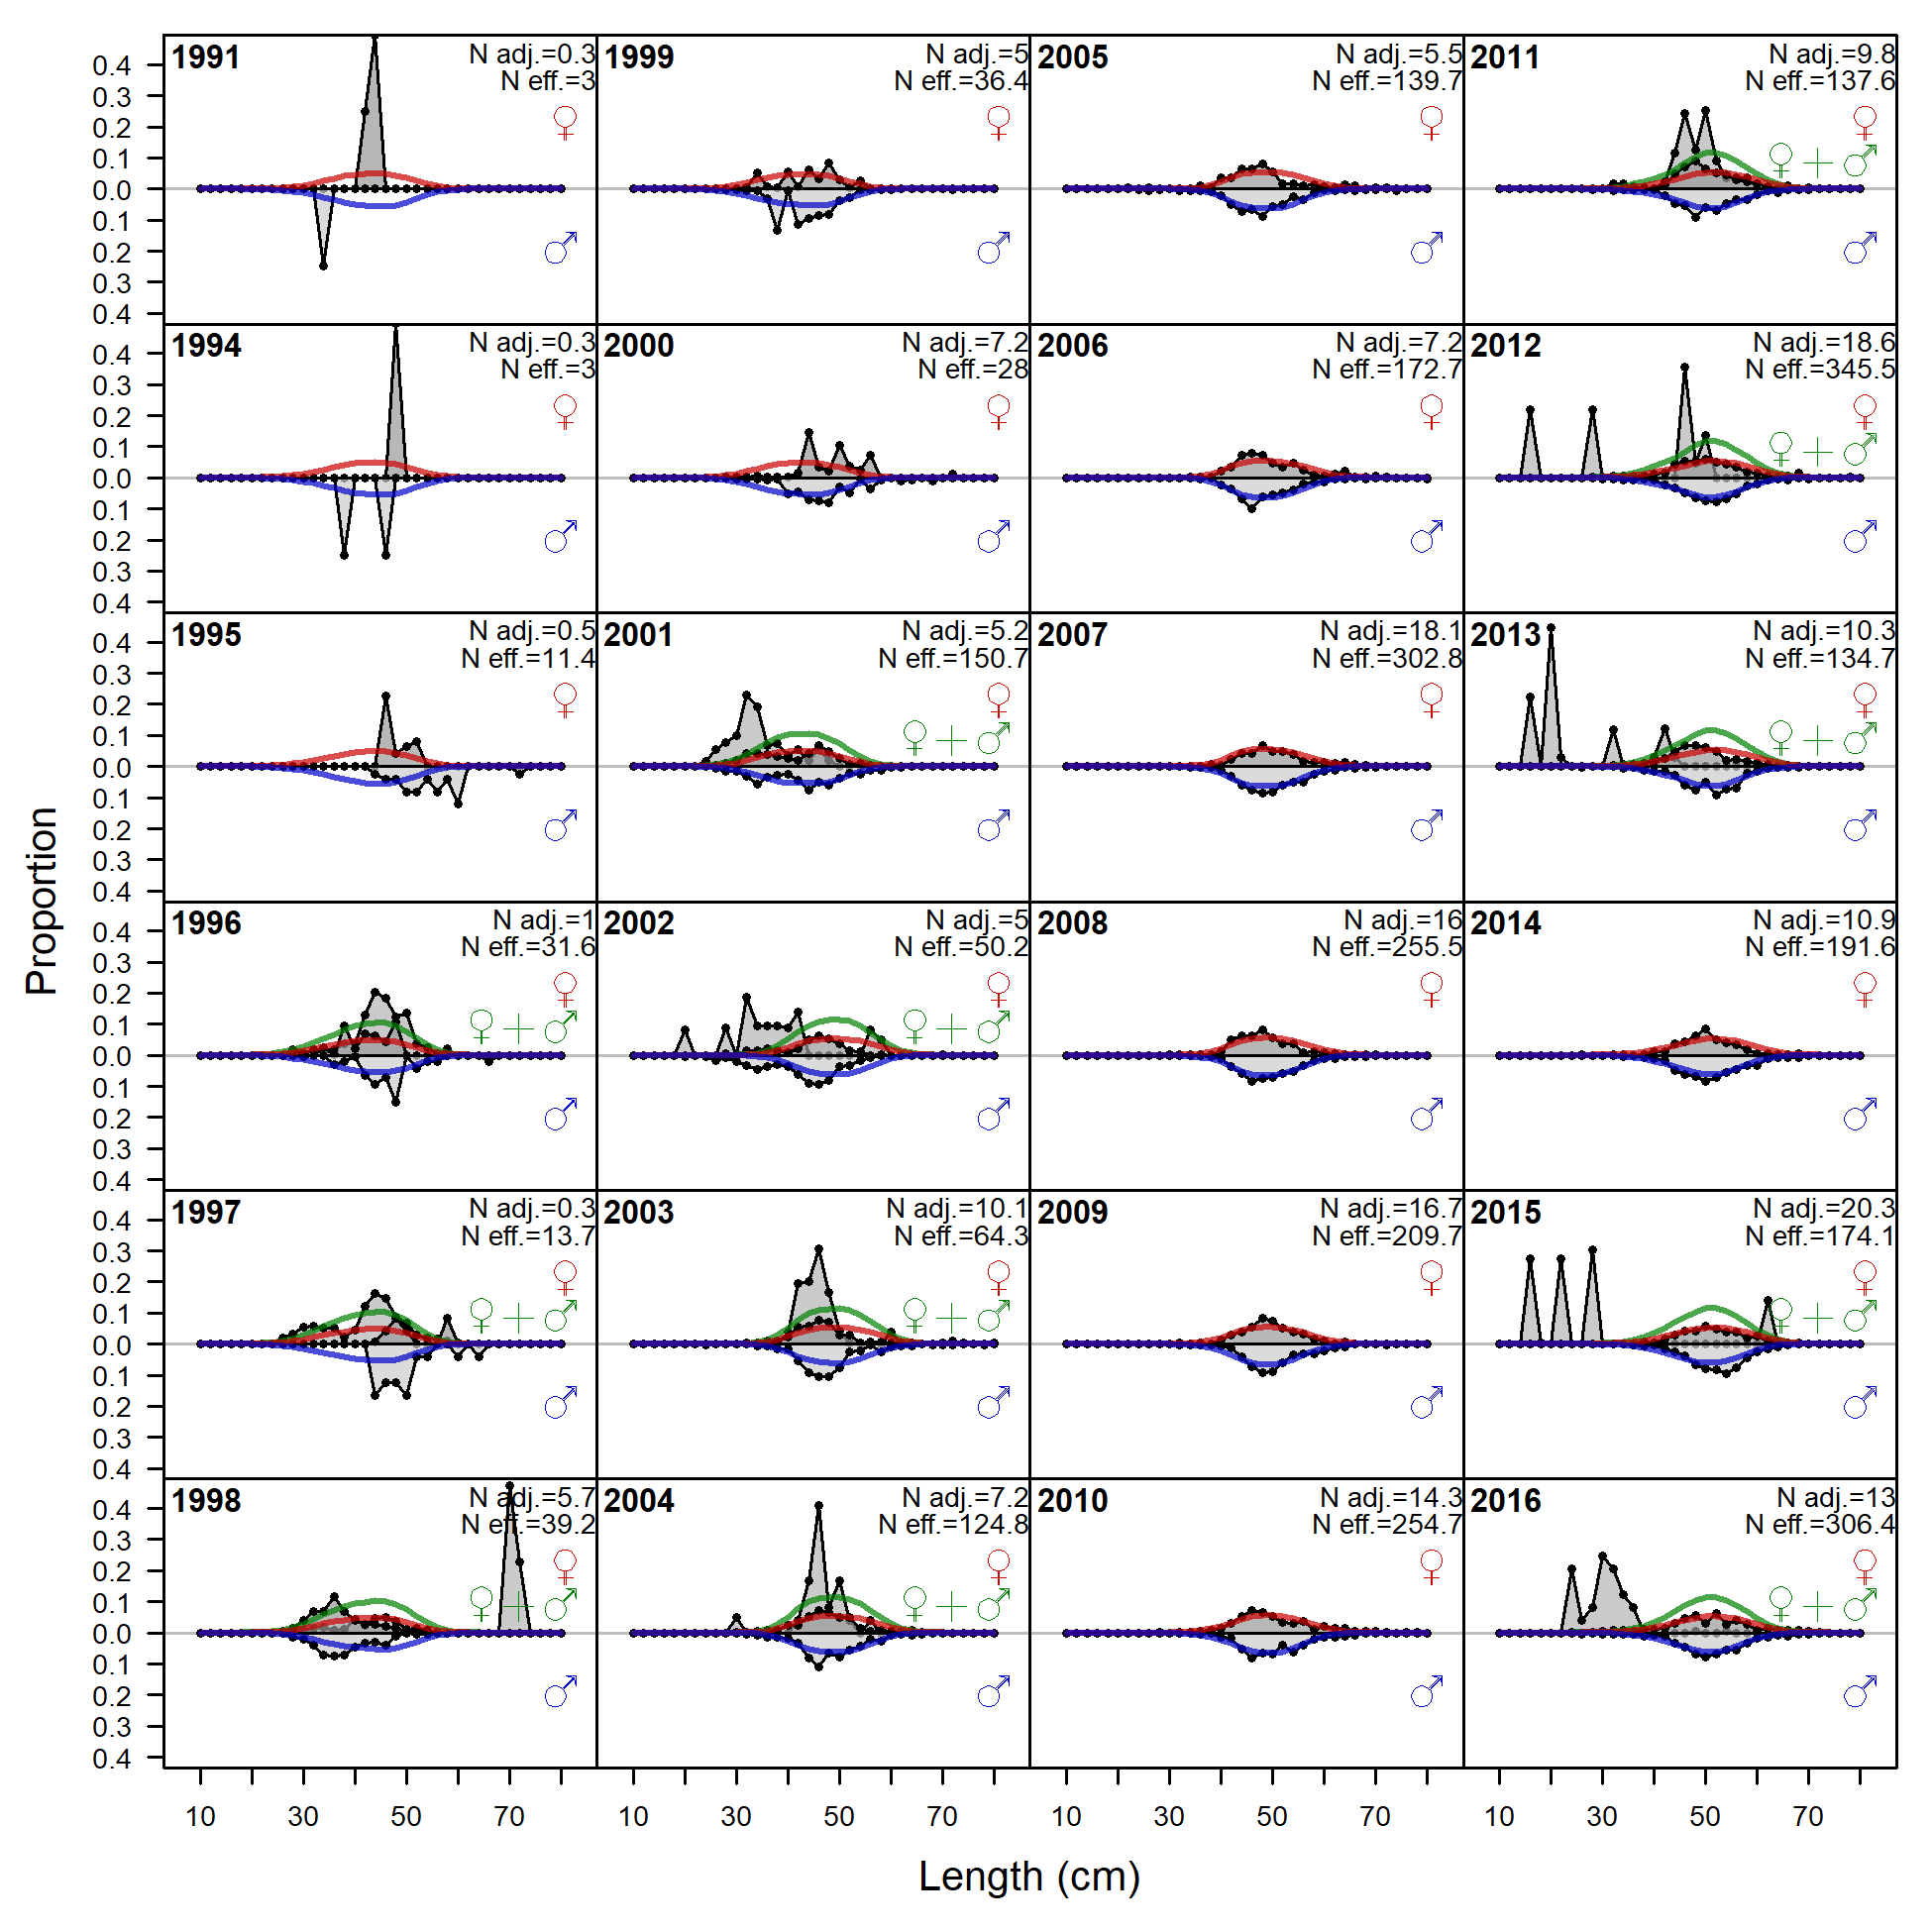
\includegraphics{ref_model/plots/comp_lenfit_flt1mkt0_page1.png}

}

\caption{\label{fig-len-fit-bt-1}Observed (gray density plot) and
expected (density lines by sex) length compositions by year for the
bottom trawl fishery in years available between 1995-2018.'N adj.' is
the input sample size after data-weighting adjustment. N eff. is the
calculated effective sample size used in the McAllister-Ianelli tuning
method.}

\end{figure}%

\begin{figure}[H]

\centering{

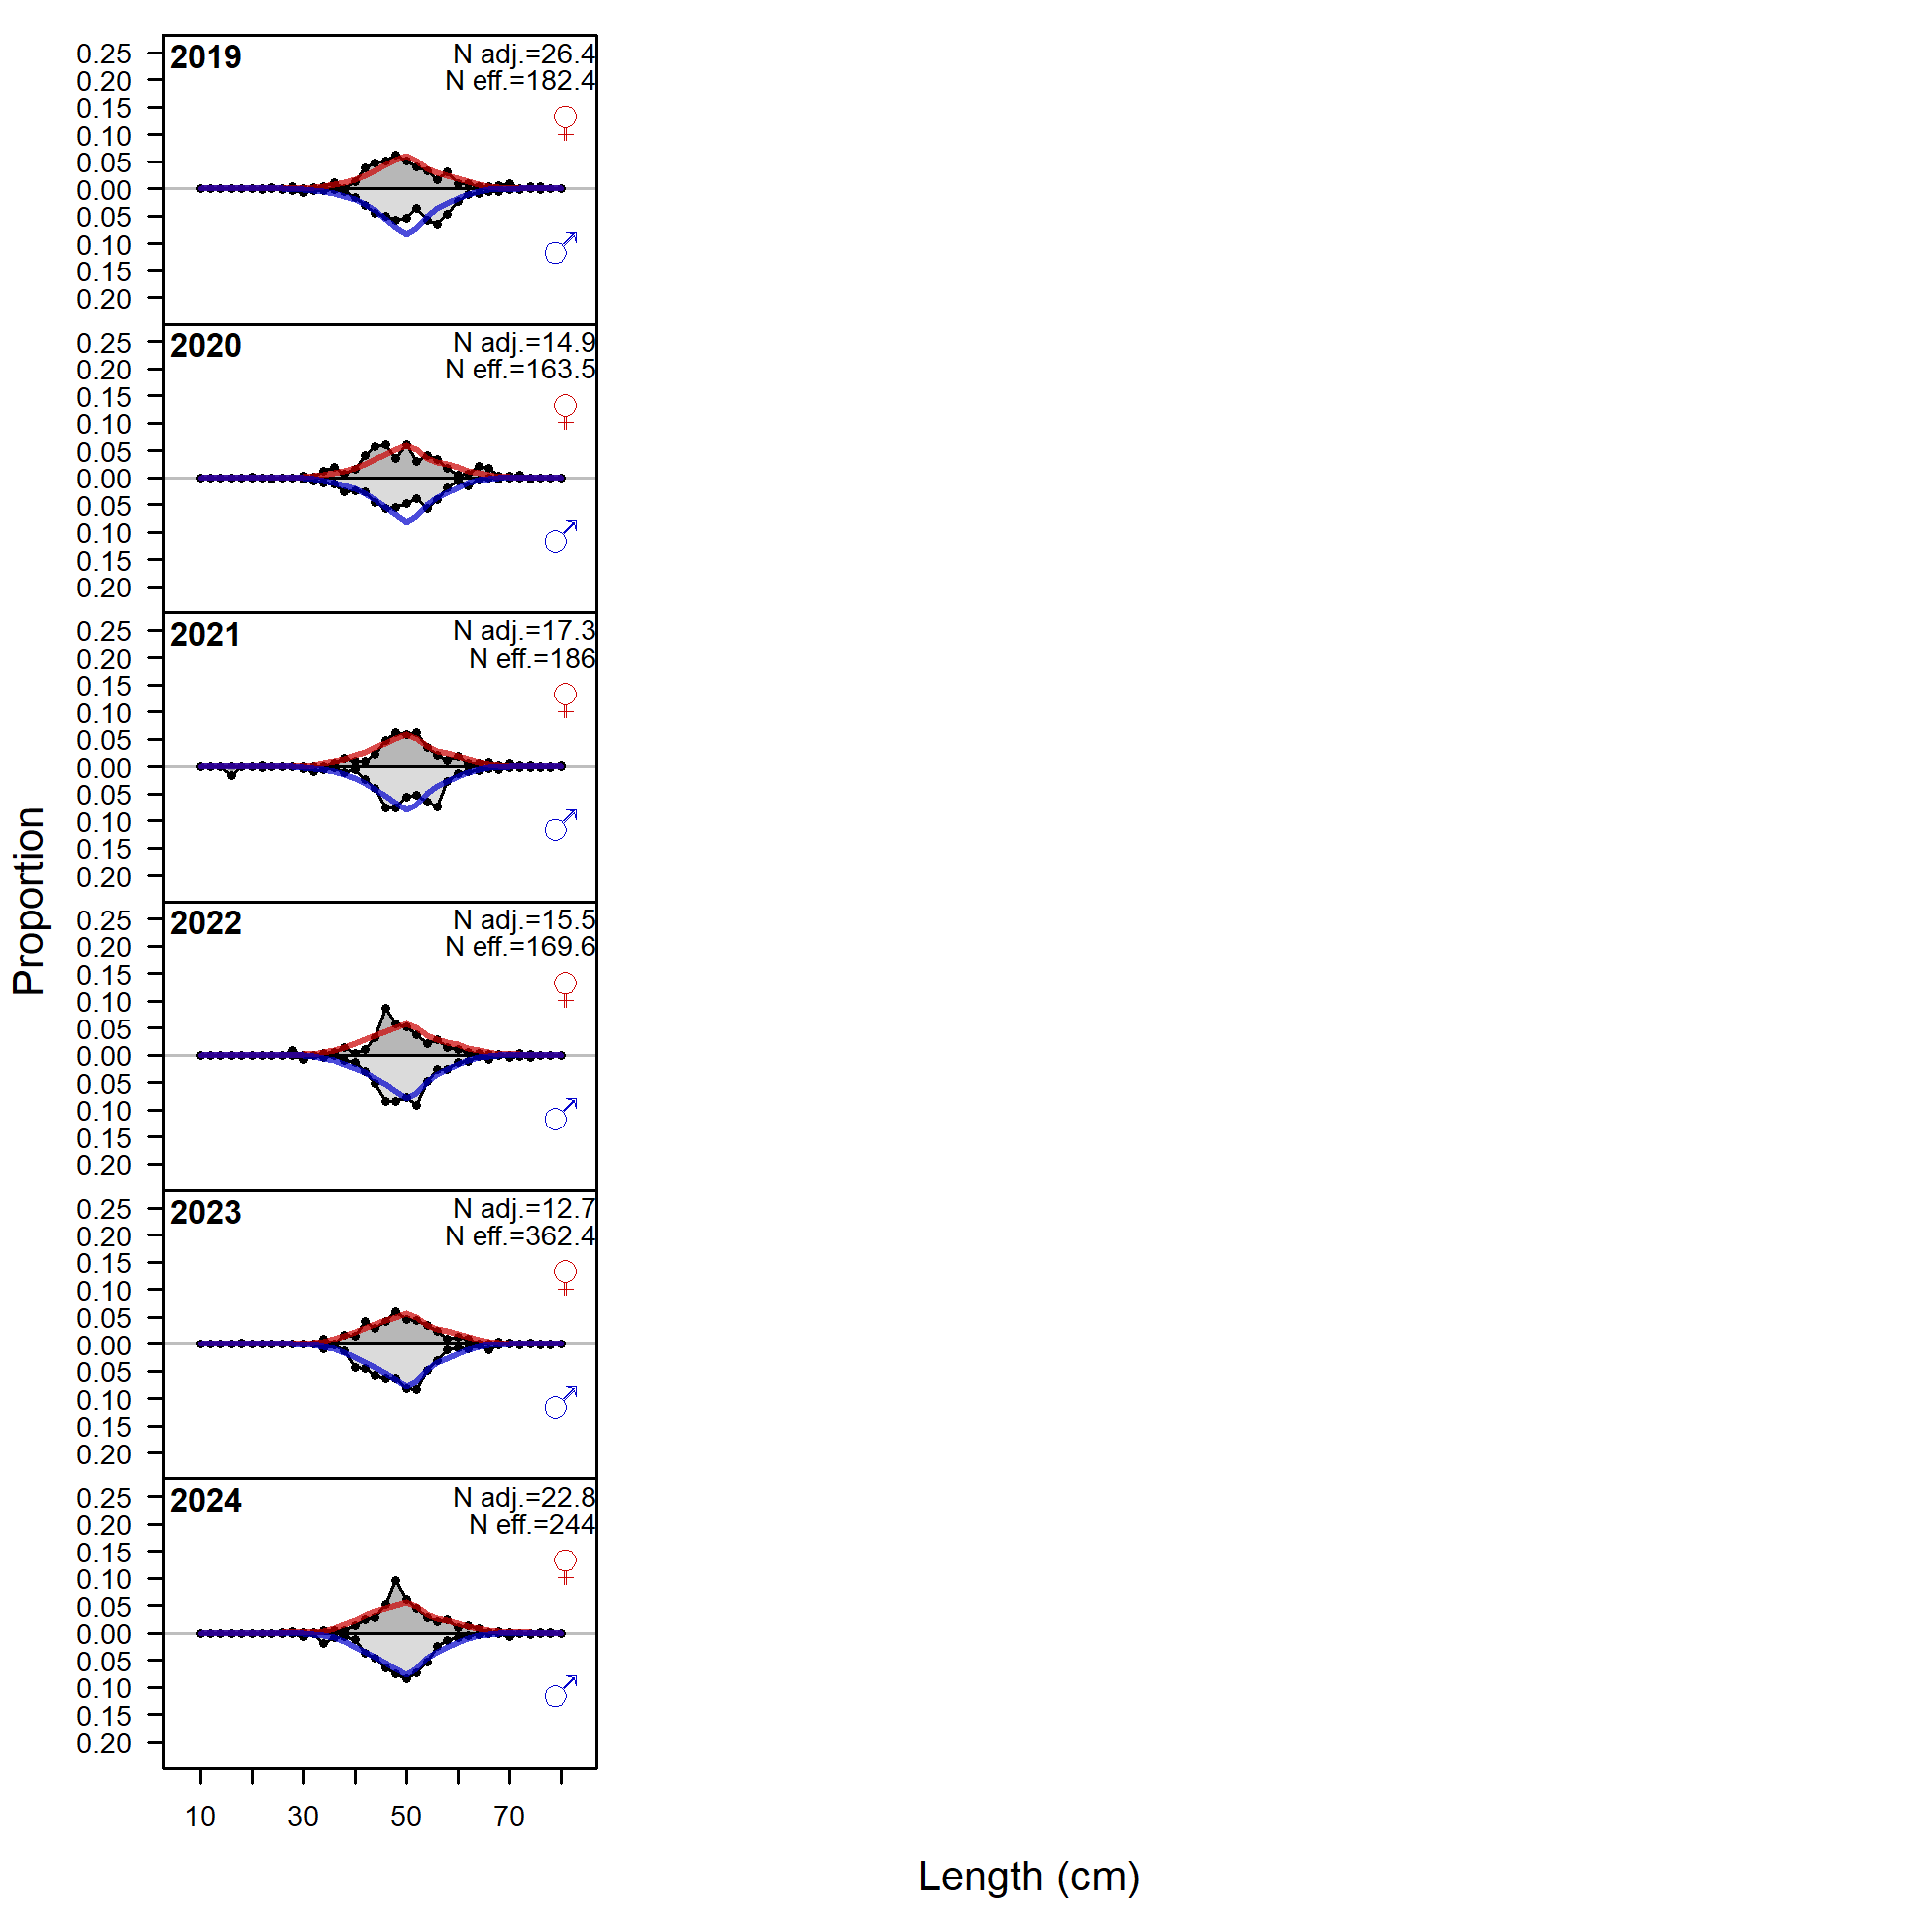
\includegraphics{ref_model/plots/comp_lenfit_flt1mkt0_page2.png}

}

\caption{\label{fig-len-fit-bt-2}Observed (gray density plot) and
expected (density lines by sex) length compositions by year for the
bottom trawl fishery in years available between 2019-2024.'N adj.' is
the input sample size after data-weighting adjustment. N eff. is the
calculated effective sample size used in the McAllister-Ianelli tuning
method.}

\end{figure}%

\begin{figure}[H]

\centering{

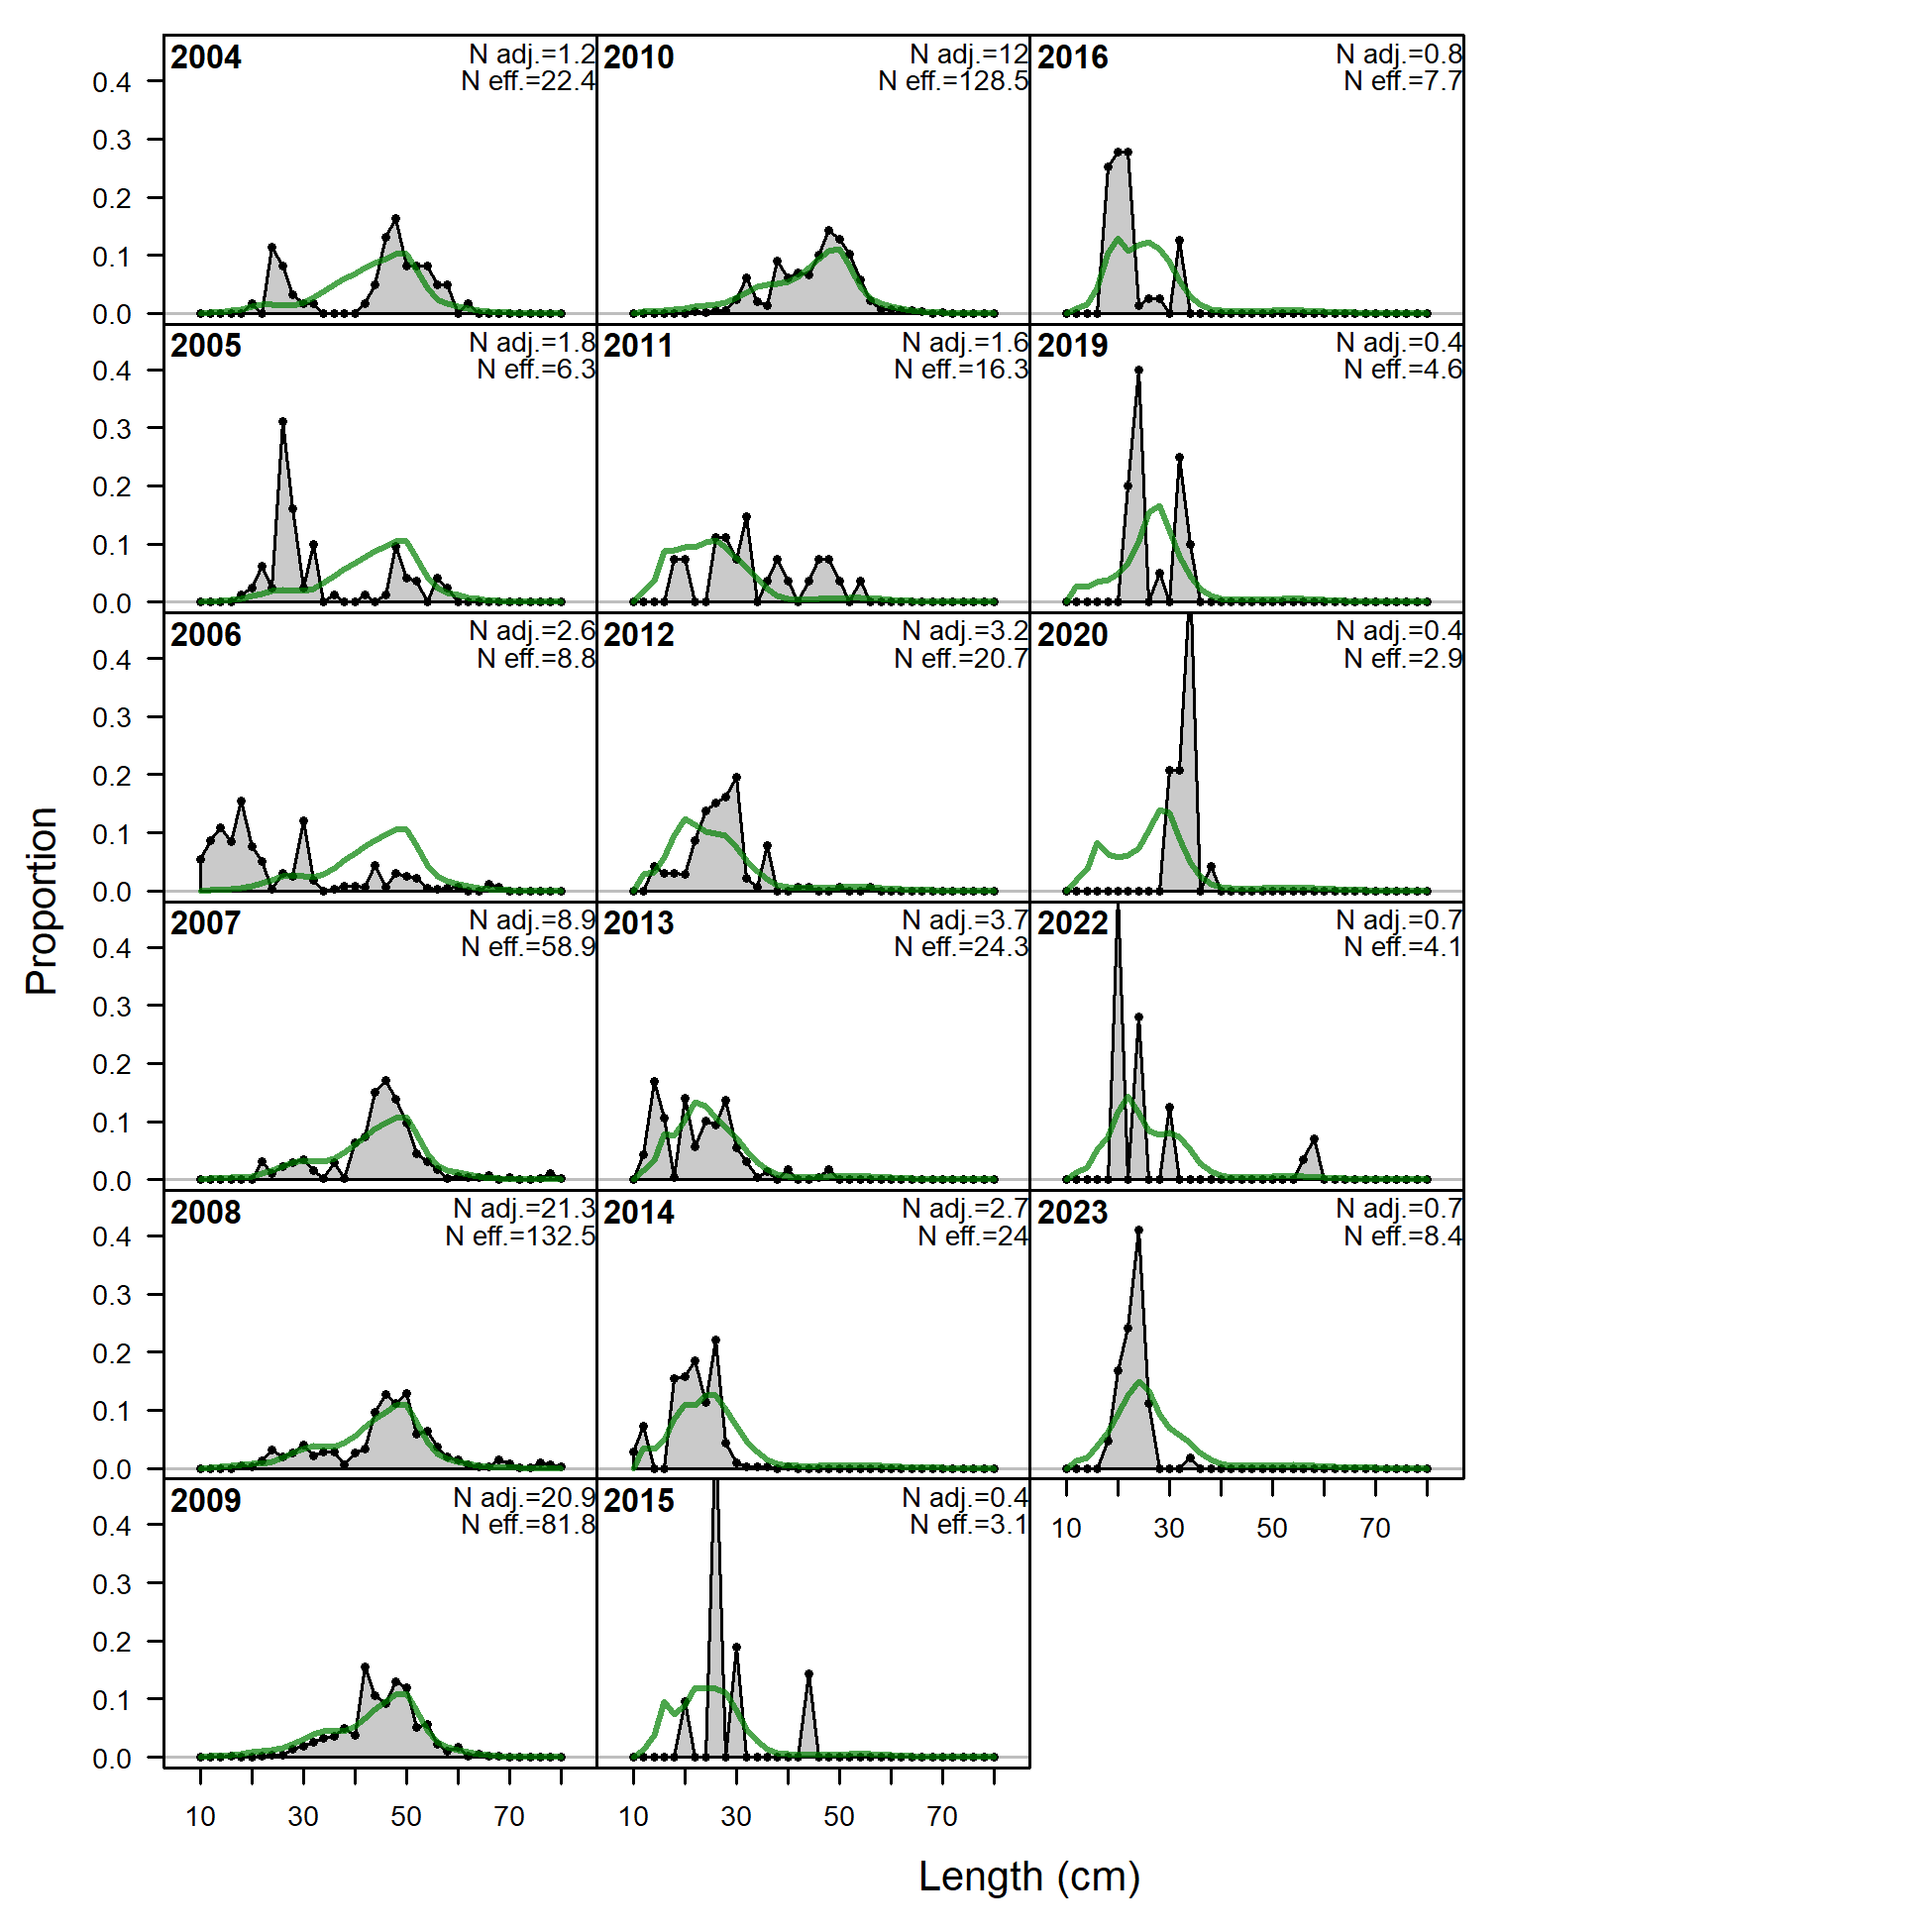
\includegraphics{ref_model/plots/comp_lenfit_flt2mkt0.png}

}

\caption{\label{fig-len-fit-btdis}Observed (gray density plot) and
expected (density lines) length compositions by year for the bottom
trawl discard fishery in years available between 2004-2023.'N adj.' is
the input sample size after data-weighting adjustment. N eff. is the
calculated effective sample size used in the McAllister-Ianelli tuning
method.}

\end{figure}%

\begin{figure}[H]

\centering{

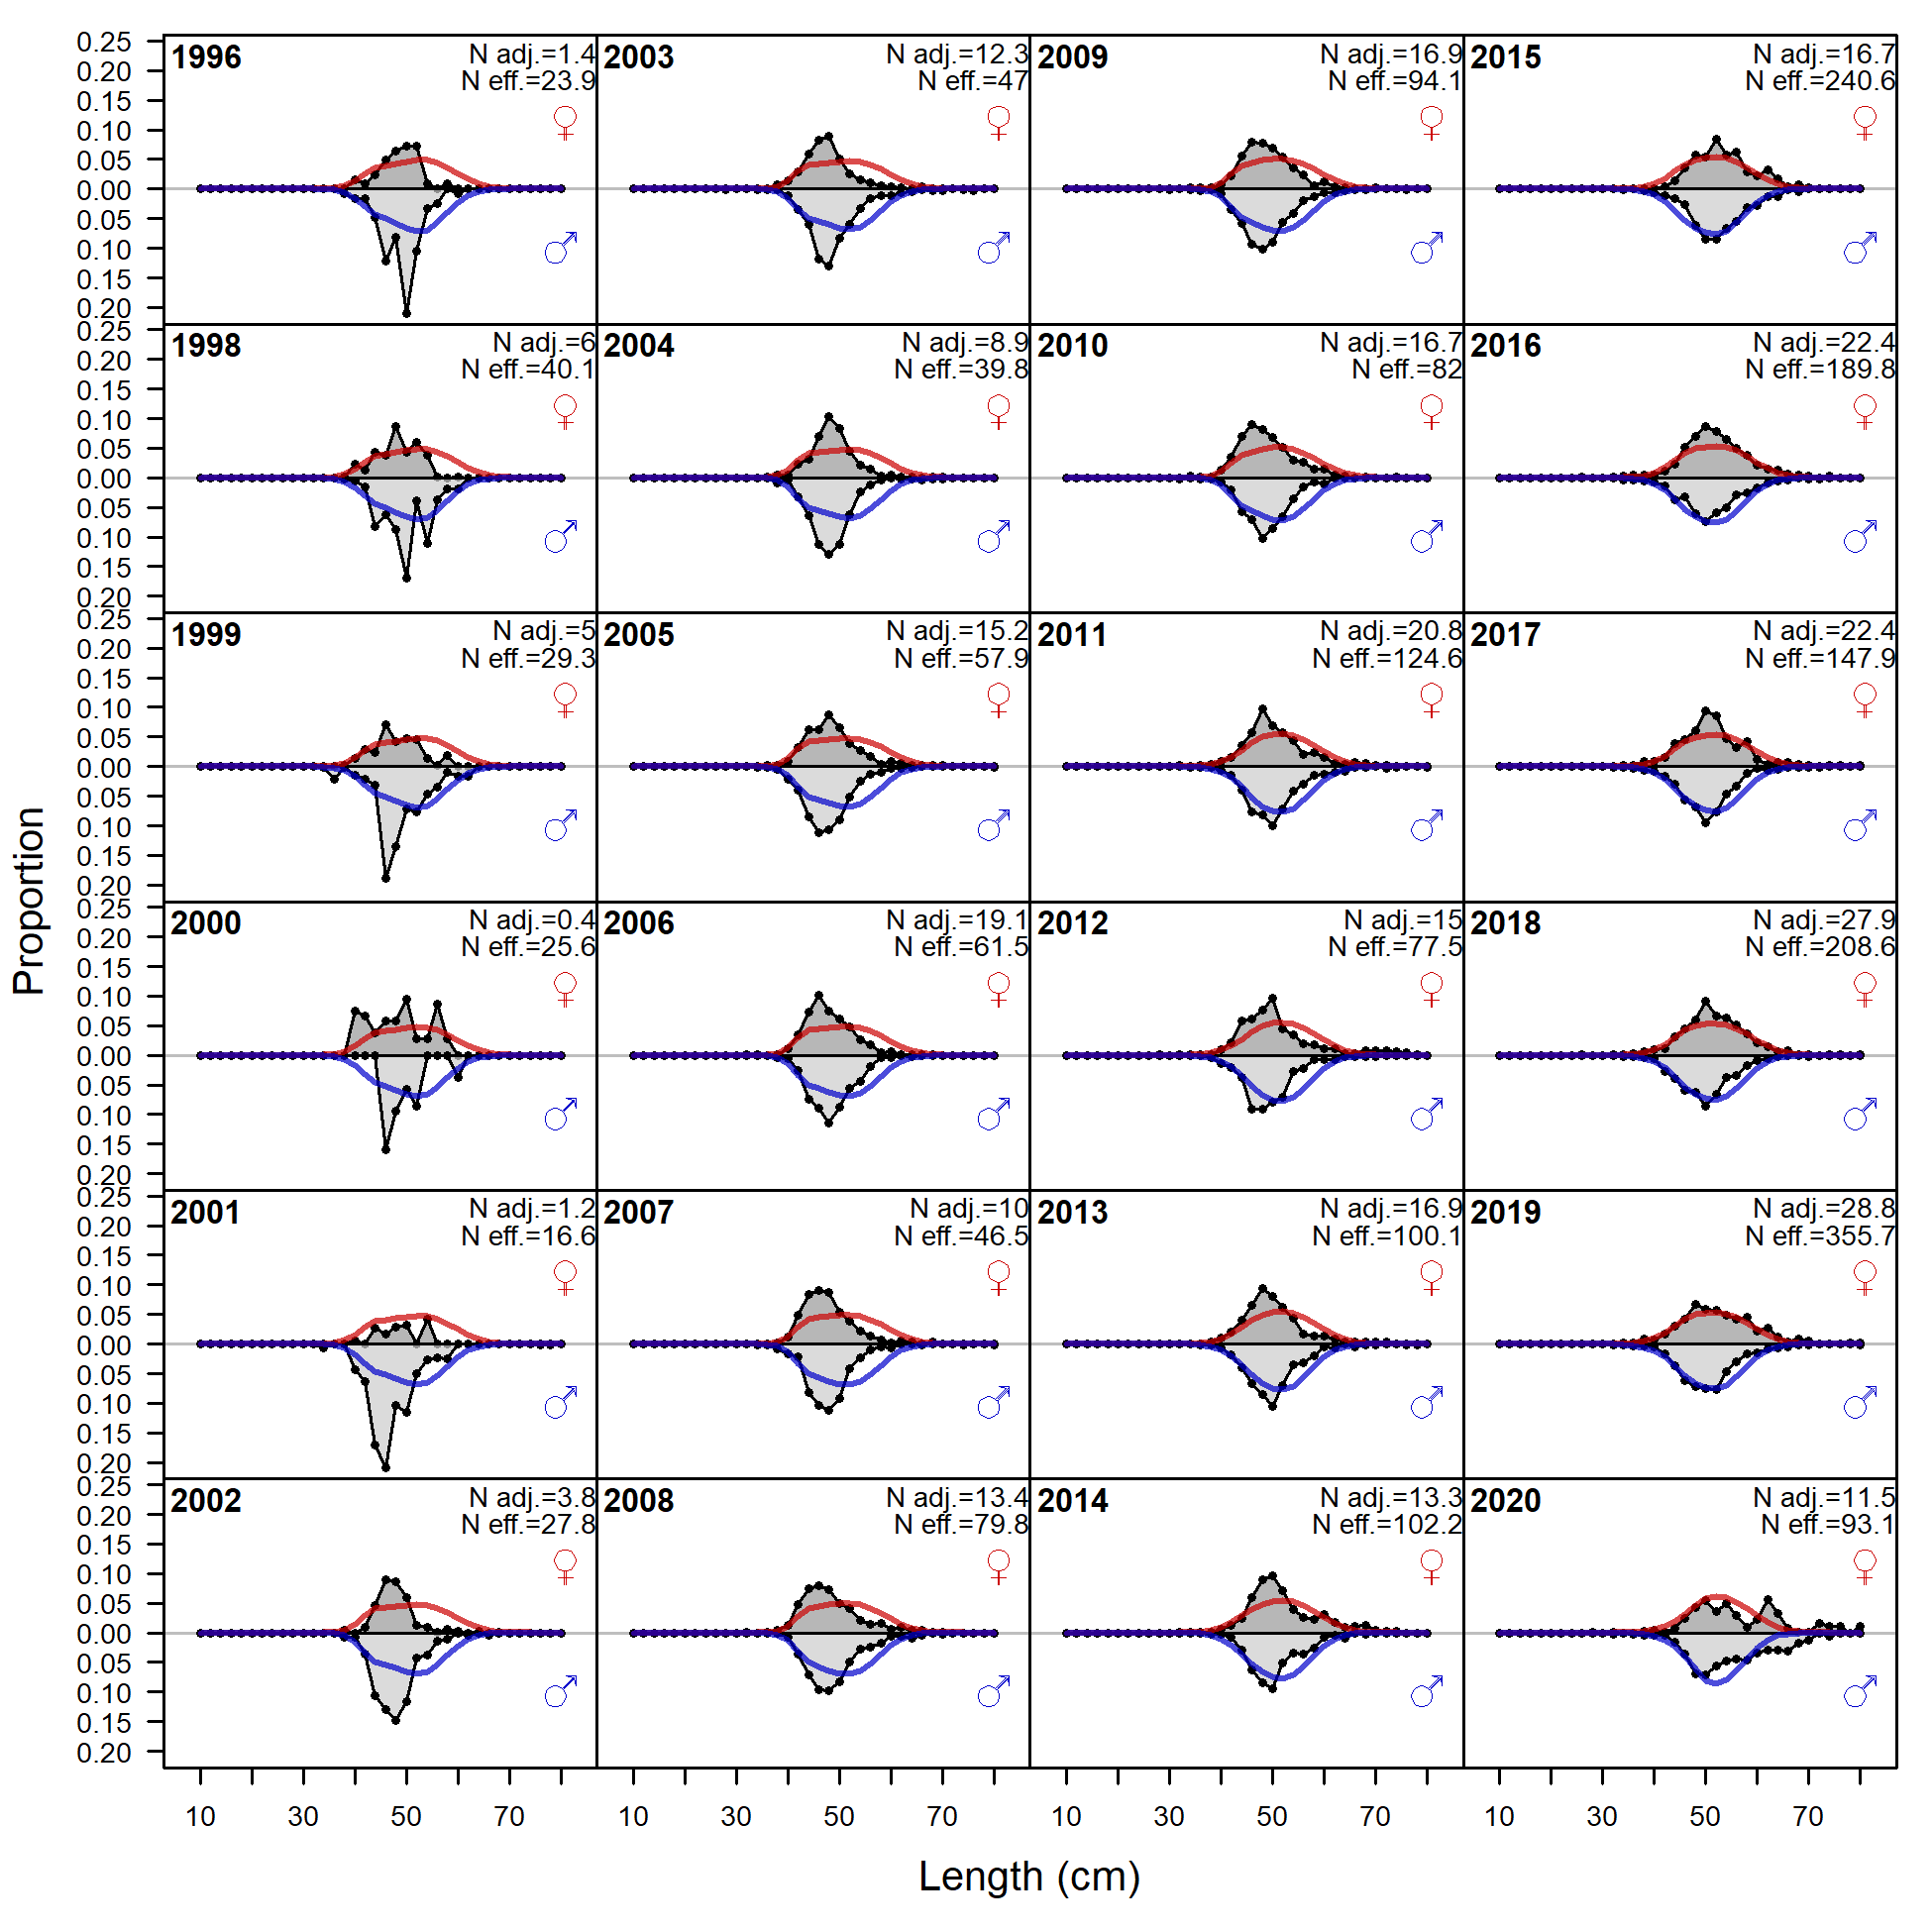
\includegraphics{ref_model/plots/comp_lenfit_flt3mkt0_page1.png}

}

\caption{\label{fig-len-fit-nt-1}Observed (gray density plot) and
expected (density lines by sex) length compositions by year for the
non-trawl fishery in years available between 1996-2020.'N adj.' is the
input sample size after data-weighting adjustment. N eff. is the
calculated effective sample size used in the McAllister-Ianelli tuning
method.}

\end{figure}%

\begin{figure}[H]

\centering{

\includegraphics{ref_model/plots/comp_lenfit_flt3mkt0_page2.png}

}

\caption{\label{fig-len-fit-nt-2}Observed (gray density plot) and
expected (density lines by sex) length compositions by year for the
non-trawl fishery in years available between 2021-2024.'N adj.' is the
input sample size after data-weighting adjustment. N eff. is the
calculated effective sample size used in the McAllister-Ianelli tuning
method.}

\end{figure}%

\begin{figure}[H]

\centering{

\includegraphics{ref_model/plots/comp_lenfit_flt4mkt0.png}

}

\caption{\label{fig-len-fit-ntdis}Observed (gray density plot) and
expected (density lines) length compositions by year for the midwater
trawl fishery in years available between 2004-2024.'N adj.' is the input
sample size after data-weighting adjustment. N eff. is the calculated
effective sample size used in the McAllister-Ianelli tuning method.}

\end{figure}%

\begin{figure}[H]

\centering{

\includegraphics{ref_model/plots/comp_lenfit_flt5mkt0.png}

}

\caption{\label{fig-len-fit-midt}Observed (gray density plot) and
expected (density lines by sex) length compositions by year for the
non-trawl discard fishery in years available between 2000-2023.'N adj.'
is the input sample size after data-weighting adjustment. N eff. is the
calculated effective sample size used in the McAllister-Ianelli tuning
method.}

\end{figure}%

\begin{figure}[H]

\centering{

\includegraphics{ref_model/plots/comp_lenfit_flt6mkt0.png}

}

\caption{\label{fig-len-fit-ashop}Observed (gray density plot) and
expected (density lines by sex) length compositions by year for the
at-sea-hake fishery in years available between 2003-2024.'N adj.' is the
input sample size after data-weighting adjustment. N eff. is the
calculated effective sample size used in the McAllister-Ianelli tuning
method.}

\end{figure}%

\begin{figure}[H]

\centering{

\includegraphics{ref_model/plots/comp_lenfit_flt7mkt0.png}

}

\caption{\label{fig-len-fit-tri}Observed (gray density plot) and
expected (density lines by sex) length compositions by year for the
Triennial Bottom Trawl Survey in years available between 1980-2004.'N
adj.' is the input sample size after data-weighting adjustment. N eff.
is the calculated effective sample size used in the McAllister-Ianelli
tuning method.}

\end{figure}%

\begin{figure}[H]

\centering{

\includegraphics{ref_model/plots/comp_lenfit_flt8mkt0.png}

}

\caption{\label{fig-len-fit-akslope}Observed (gray density plot) and
expected (density lines by sex) length compositions by year for the
Alaskan Slope Bottom Trawl Survey in years available between
1997-2001.'N adj.' is the input sample size after data-weighting
adjustment. N eff. is the calculated effective sample size used in the
McAllister-Ianelli tuning method.}

\end{figure}%

\begin{figure}[H]

\centering{

\includegraphics{ref_model/plots/comp_lenfit_flt10mkt0.png}

}

\caption{\label{fig-len-fit-wcgbts}Observed (gray density plot) and
expected (density lines by sex) length compositions by year for the West
Coast Groundfish Bottom Trawl Survey in years available between
1980-2004.'N adj.' is the input sample size after data-weighting
adjustment. N eff. is the calculated effective sample size used in the
McAllister-Ianelli tuning method.}

\end{figure}%

\newpage

\subsection{Model outputs}\label{model-outputs}

\begin{figure}[H]

\centering{

\includegraphics{ref_model/plots/ts7_Spawning_output_with_95_intervals.png}

}

\caption{\label{fig-sb}Estimated time series of spawning output for the
base model.}

\end{figure}%

\begin{figure}[H]

\centering{

\includegraphics{ref_model/plots/ts9_Relative_spawning_output_intervals.png}

}

\caption{\label{fig-depl}Estimated time series of fraction of unfished
spawning output for the base model.}

\end{figure}%

\begin{figure}[H]

\centering{

\includegraphics{ref_model/plots/ts11_Age-0_recruits_(1000s)_with_95_asymptotic_intervals.png}

}

\caption{\label{fig-recruits}Estimated time series of age-0 recruits for
the base model.}

\end{figure}%

\pagebreak

\begin{figure}[H]

\centering{

\includegraphics{ref_model/plots/recdevs2_withbars.png}

}

\caption{\label{fig-recdevs}Estimated time series of recruitment
deviations for the base model.}

\end{figure}%

\begin{figure}[H]

\centering{

\includegraphics{ref_model/plots/recruit_fit_bias_adjust.png}

}

\caption{\label{fig-biasramp}Bias adjustment applied to the recruitment
deviations (red line). Points are transformed variances relative to the
assumed variance of recruitment.}

\end{figure}%

\begin{figure}[H]

\centering{

\includegraphics{ref_model/plots/SPR3_ratiointerval.png}

}

\caption{\label{fig-spr}Estimated time series of fishing intensity for
the base model.}

\end{figure}%

\begin{figure}[H]

\centering{

\includegraphics{ref_model/plots/SPR4_phase.png}

}

\caption{\label{fig-spr-phase}Phase plot of fishing intensity versus
fraction unfished for the base model.}

\end{figure}%

\begin{figure}[H]

\centering{

\includegraphics{ref_model/plots/yield2_yield_curve_with_refpoints.png}

}

\caption{\label{fig-yield}Estimated yield curve with reference points
for the base model.}

\end{figure}%

\begin{figure}[H]

\centering{

\includegraphics{ref_model/plots/ts_DynamicB0.png}

}

\caption{\label{fig-dyn-b0}Dynamic B0 plot. The lower line shows the
time series of estimated spawning output in the presence of fishing
mortality. The upper line shows the time series that could occur under
the same dynamics (including deviations in recruitment), but without
fishing. The point at the left represents the unfished equilibrium.}

\end{figure}%

\newpage

\subsection{Sensitivity Analyses and
Retrospectives}\label{sensitivity-analyses-and-retrospectives}

\newpage

\subsection{Likelihood Profiles}\label{likelihood-profiles-1}

\newpage

\subsection{Reference Points and
Forecasts}\label{reference-points-and-forecasts}

\newpage

\newpage{}

\section{Notes}\label{notes}

\newpage{}

\section{Appendices}\label{sec-appendix}




\end{document}
